\documentclass[11pt, a4paper]{article}

\usepackage{style}

\institution{EPFL}
\project{Semester Project}
\title{Minimal Rational Interpolation for Time-Harmonic Maxwell's Equations}
\author{Fabio Matti}
\supervisor{Prof. Fabio Nobile \\ Dr. Davide Pradovera}
\date{\today}

\begin{document}

\maketitle

\begin{abstract}
    \acrfull{MRI} provides an efficient and reliable way to approximate the 
    dependence of a characteristic quantity of a model on one of its parameters.
    The focus of this report is put on the \acrfull{gMRI} algorithm and particularly
    on way to enhance its performance. This algorithm is then applied to three 
    example problems concerning the time-harmonic Maxwell's equations in the 
    frequency domain. A brief evaluation of the advantages and disadvantages of
    \acrshort{gMRI} as compared to conventional approaches for finding quantities,
    such as resonant modes, of interest for problems of this type is conducted.
\end{abstract}

%\newpage
%\printglossary[type=\acronymtype, nonumberlist]

\newpage
\tableofcontents

\newpage
\section{Introduction}
\label{sec:introduction}

A wide class of problems in physics and engineering concerns itself with the
study of the dependence of a model on one of its parameters. 
Of interest is usually a characteristic quantity that covaries with said parameter.
Unless the system allows for an analytical solution, one may usually only
find numerical solutions to the system for discrete values of the parameter.
\acrfull{MRI} offers a way to locally approximate the continuous
dependence of a model on one of its parameters. The approach has proven
effective and efficient (both memory- and computation wise) in applications
on Helmholtz-type problems \cite{greedyMRI, shortMRI}.

Central to this report are time-harmonic electromagnetic problems, whose 
parameter is the (angular) frequency. These problems are governed by
the time-harmonic Maxwell's equations. Choosing the quantity of interest
to be a vector potential, these equations reduce to a single curl-curl equation.
A justification for why a rational interpolation approach is appropriate for
this class of problems will be presented in Section \ref{subsec:motivation}.

The first few pages in this report are a short guide for finding numerical 
solutions to the time-harmonic Maxwell's equations using the \acrfull{FEM}.
These solutions are then used in the core of this report, which gives a description
of the \acrfull{gMRI} algorithm. Properties of and optimization tricks for the
\acrshort{gMRI} are shown. In the end, three applications of the method are studied and
discussed: the resonant modes of a two-dimensional resonant cavity,
the two-dimensional cavity with an imperfectly conducting boundary, and lastly
the scattering coefficients of a \acrfull{DMCWF}.

\newpage
\section{Finite element discretization of the time-harmonic Maxwell's equations}
\label{sec:maxwell}

\acrfull{MRI} requires the knowledge of the solution of the problem for multiple 
values of the model parameter that is of interested. A way of obtaining these
solutions is the \acrfull{FEM}. For that purpose, I now derive a strong formulation
for the time-harmonic Maxwell problem and subsequently convert it to its
corresponding weak formulation.

\subsection{Vector potential formulation of the time-harmonic Maxwell's equations}
\label{subsec:maxwell-potential}

% Everything smooth enough to do all manipulations...
I assume that all quantities in this section are smooth enough to perform the
necessary vector calculus manipulations.

Let $\mathbf{E}$ denote an electric field, $\mathbf{B}$ a magnetic field
strength, $\rho$ an electric charge density, and $\mathbf{j}$ an electric
current density. Maxwell's equations are stated in \citep{monk} as
\begin{align}
    \nabla \cdot (\epsilon \mathbf{E}) &= \rho \label{equ:maxwell1} \\
    \nabla \cdot \mathbf{B} &= 0 \label{equ:maxwell2} \\
    \nabla \times \mathbf{E} &= -\partial_t \mathbf{B} \label{equ:maxwell3} \\
    \nabla \times (\mu^{-1} \mathbf{B}) &= \partial_t (\epsilon \mathbf{E}) + \mathbf{j} \label{equ:maxwell4}
\end{align}
with $\varepsilon$ being the permittivity and $\mu$ the permeability (whose names 
let alone their values I always tend to forget).

% Non-conducting material, else => j = sigma*E + J_a (Monk 21)

Equation (\ref{equ:maxwell2}) motivates the expression of the magnetic field 
$\mathbf{B} = \nabla \times \mathbf{u}$ in terms of a vector-valued function
$\mathbf{u}$, the vector potential (in literature commonly denoted with
$\mathbf{A}$). Similarly, (\ref{equ:maxwell3}) suggests
rewriting the electric field $\mathbf{E} = - \nabla \phi - \partial_t \mathbf{u}$
using a scalar function $\phi$, referred to as the scalar potential.

The physical quantities $\mathbf{E}$ and $\mathbf{B}$ remain unchanged 
if we transform $\mathbf{u} \to \mathbf{u}' = \mathbf{u} + \nabla \psi$ or
$\phi \to \phi' = \phi - \partial_t \psi$ for arbitrary functions $\psi$.
A convenient choice of $\psi$ is suggested in \citep{gauge-transformation} to be
\begin{equation}
    \psi = \int_0^t \phi dt' \label{equ:gauge}
\end{equation}
which transforms $\phi \to \phi' = 0$ and $\mathbf{u} \to \mathbf{u}' = \mathbf{u}
+ \nabla \int_0^t \phi dt'$. Thus, the expressions for the electrical and
magnetic field become
\begin{align}
    \mathbf{E} &= -\partial_t \mathbf{u} \label{equ:electricfield} \\
    \mathbf{B} &= \nabla \times \mathbf{u} \label{equ:magneticfield}
\end{align}
where I have subtly renamed the variable $\mathbf{u}'$ to $\mathbf{u}$ for simplicity.

Plugging the identities (\ref{equ:electricfield}) and (\ref{equ:magneticfield})
into (\ref{equ:maxwell4}) yields 
\begin{equation}
    \nabla \times (\mu^{-1} \nabla \times \mathbf{u}) = - \epsilon \partial_t^2 \mathbf{u} + \mathbf{j} \label{equ:maxwell-potential}
\end{equation}

For the rest of this report, I restrict myself to vector potentials $\mathbf{u}$
that exhibit a harmonic dependence on time $t$, i.e. may be factorized into
a term solely depending on the position $\mathbf{x}$ and a complex exponential
depending on time
\begin{equation}
    \mathbf{u}(\mathbf{x}, t) = \mathbf{u}(\mathbf{x}) \exp(i \omega t) \label{equ:time-harmonic}
\end{equation}
Substituting this expression into (\ref{equ:maxwell-potential}) and rearranging 
a little results in the
\begin{fancybox}{Time-harmonic potential equation}
    \begin{equation}
     \nabla \times (\mu^{-1} \nabla \times \mathbf{u}) - \epsilon \omega^2 \mathbf{u} = \mathbf{j} \label{equ:maxwell-timeharmonic}
    \end{equation}
\end{fancybox}

\subsection{Weak formulation for the time-harmonic potential equation}
\label{subsec:maxwell-weak}

Equation (\ref{equ:maxwell-timeharmonic}) may be multiplied by a vector-valued
function $\mathbf{v} \in H_{\textrm{curl}}(\Omega)$, where
\begin{equation}
    H_{\textrm{curl}}(\Omega) = \{\mathbf{u} : \Omega \to \mathbb{C},~\text{such that}~\mathbf{u}\in L_2(\mathbb{C})^3, \nabla \times \mathbf{u} \in L_2(\mathbb{C})^3\} \label{equ:h-curl}
\end{equation}
and then integrated over the whole computational domain $\Omega$ to obtain 
\begin{equation}
    \int_{\Omega} (\nabla \times ({\mu^{-1} \nabla \times \mathbf{u}})) \cdot \mathbf{v}
    - \omega^2 \int_{\Omega} \epsilon \mathbf{u} \cdot \mathbf{v} = \int_{\Omega} \mathbf{j} \cdot \mathbf{v} \label{equ:maxwell-weak-initial}
\end{equation}
This may further be simplified (\ref{equ:maxwell-weak-initial}) to (I allow myself
to spare you the details of this computation, but put a proper derivation
in an appendix at the end of the report):
\begin{fancybox}{Weak formulation of the time-harmonic potential equation}
    \begin{equation}
        \int_{\Omega} ({\mu^{-1} \nabla \times \mathbf{u}}) \cdot (\nabla \times \mathbf{v})
        - \omega^2 \int_{\Omega} \epsilon \mathbf{u} \cdot \mathbf{v} 
        = \int_{\Omega} \mathbf{j} \cdot \mathbf{v}
        + \int_{\partial \Omega} \underbrace{(({\mu^{-1} \nabla \times \mathbf{u}}) \times \mathbf{n})}_{= \mathbf{g}} \cdot \mathbf{v}
        \label{equ:maxwell-weak}
    \end{equation}
\end{fancybox}
where $\mathbf{n}$ denotes the surface normal to the boundary $\partial \Omega$
of the computational domain $\Omega$.

Boundary conditions on the electric field $\mathbf{E}$ may be most easily enforced
in a Dirichlet-type fashion through the relation (\ref{equ:electricfield}) and
the assumption (\ref{equ:time-harmonic})
\begin{equation}
    \left.\mathbf{u}\right|_{\Gamma_D} = -\frac{1}{i\omega} \left.\mathbf{E}\right|_{\Gamma_D} \label{equ:dirichlet-boundary}
\end{equation}
Those on the magnetic field $\mathbf{B}$ through a Neumann-type condition following
from (\ref{equ:magneticfield}) and again (\ref{equ:time-harmonic})
\begin{equation}
    \left.\mathbf{g}\right|_{\Gamma_N} = (\mu^{-1} \left.\mathbf{B}\right|_{\Gamma_N}) \times \mathbf{n} \label{equ:neumann-boundary}
\end{equation}

\subsection{Examples}
\label{subsec:examples}

I will now specialize and simplify this weak formulation for three different
applications which will be studied in Section \ref{sec:examples}. To show you
that these problems are intimately related problems, I refer you to Figure \ref{fig:examples}.

\begin{figure}[h]
    \centering
    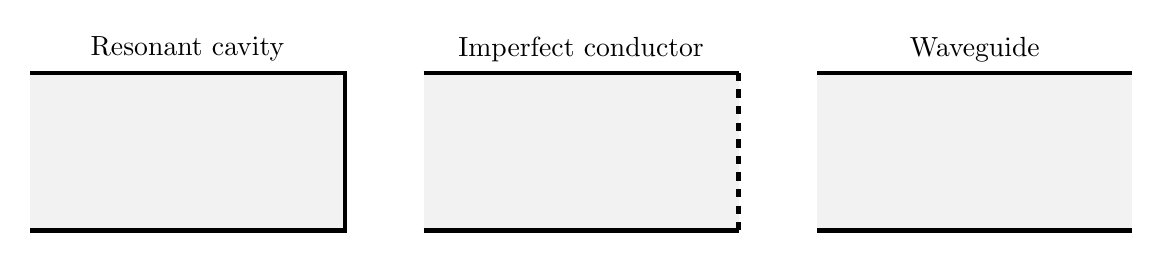
\begin{tikzpicture}
    \node at (2, 2.3) {Resonant cavity};
    \fill[black!5!white] (0, 0) rectangle (4, 2);
    \draw[ultra thick] (0, 0) to (4, 0) to (4, 2) to (0, 2);

    \node at (7, 2.3) {Imperfect conductor};
    \fill[black!5!white] (5, 0) rectangle (9, 2);
    \draw[ultra thick] (5, 0) to (9, 0);
    \draw[ultra thick, dashed] (9, 2) to (9, 0);
    \draw[ultra thick] (5, 2) to (9, 2);

    \node at (12, 2.3) {Waveguide};
    \fill[black!5!white] (10, 0) rectangle (14, 2);
    \draw[ultra thick] (10, 0) to (14, 0);
    \draw[ultra thick] (10, 2) to (14, 2);
\end{tikzpicture}
    \caption{Schematic visualization of the most trivial case for each of the
    boundary configurations that will be analyzed in Section \ref{sec:examples}.
    The perfectly conducting boundaries are drawn in black, while the imperfectly
    conducting boundary appears dashed. Inlets and exits are left unmarked.}
    \label{fig:examples}
\end{figure}

\subsubsection{Two-dimensional resonant cavity}
\label{subsubsec:cavity}

I refer to a resonant cavity as a region $\Omega$ enclosed by a boundary $\partial \Omega$.
The boundary can be subdivided into one (or more) inlets $\Gamma_N$ and a perfect
conducting wall $\Gamma_D = \partial \Omega \setminus \Gamma_N$
(see Figure \ref{fig:2d-cavity} for an abstract visualization of such a cavity).

\begin{figure}[h]
    \centering
    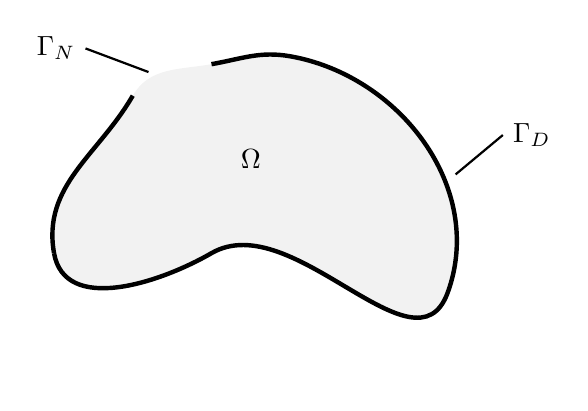
\begin{tikzpicture}
    \fill[black!5!white] (2, 1) to [out=100, in=240] (3, 3)
                              to [out=60, in=190] (4, 3.4)
                              to [out=10, in=170] (5, 3.5)
                              to [out=350, in=70] (7, 0.5)
                              to [out=250, in=30] (4, 1)
                              to [out=210, in=280] (2, 1);
    \draw[ultra thick] (2, 1) to [out=100, in=240] (3, 3);

    \draw[ultra thick] (4, 3.4) to [out=10, in=170] (5, 3.5)
                              to [out=350, in=70] (7, 0.5)
                              to [out=250, in=30] (4, 1)
                              to [out=210, in=280] (2, 1);
    \draw[thick] (2.4, 3.6) node[left] {$\Gamma_N$} to (3.2, 3.3);
    \draw[thick] (7.7, 2.5) node[right] {$\Gamma_D$} to (7.1, 2);
    \node at (4.5, 2.2) {$\Omega$};
\end{tikzpicture}
    \caption{An abstract example of a two-dimensional resonant cavity enclosing
    a domain $\Omega$ with a perfectly conducting boundary $\Gamma_D$ and
    featuring a single inlet $\Gamma_N$.}
    \label{fig:2d-cavity}
\end{figure}

Suppose the current density $\mathbf{j} \equiv 0$ and orient the coordinate
system in such a way that $\mathbf{u} = u_z \mathbf{e}_z$ and 
$\mathbf{v} = v_z \mathbf{e}_z$. Consequently, the scalar product of the two 
curls in Equation (\ref{equ:equ:maxwell-weak}) simplifies to the scalar product 
of two gradients:
\begin{equation}
    (\mu^{-1} \nabla \times \mathbf{u}) \cdot (\nabla \times \mathbf{v})
    = (\mu^{-1} \nabla u_z) \cdot (\nabla v_z)
\end{equation}
Denote by $g_z$ the component of $\mathbf{g}$ in the $z$-direction along the
inlet $\Gamma_N$. These simplifications allow the conversion of 
(\ref{equ:maxwell-weak}) into the weak formulation for a two-dimensional
resonant cavity
\begin{equation}
    \int_{\Omega} (\mu^{-1} \nabla u_z) \cdot (\nabla v_z)
    - \omega^2 \int_{\Omega} \epsilon u_z v_z
    = \int_{\partial \Omega} g_z v_z \label{equ:maxwell-weak-resonant-cavity}
\end{equation}

% Boundary conditions Dirichlet and Neumann (from Monk)
Now, let $\mathbf{E}$ and $\mathbf{B}$ refer to the electric and magnetic fields inside
the cavity. For now, I distinguish between two types of boundaries:

For the perfectly conducting boundary $\Gamma_D$, treated in \citep{monk}, it holds that
\begin{equation}
    \mathbf{n} \times \mathbf{E} = 0,~~\text{on}~\Gamma_D \label{equ:perfect-conductor-boundary}
\end{equation}
For the boundaries in a two-dimensional resonant cavity (see Figure 
\ref{fig:2d-cavity}), this only holds true if $E_z = 0$, which translates
to the Dirichlet boundary condition $\left.\mathbf{u}\right|_{\Gamma_D} = 0$
in light of (\ref{equ:dirichlet-boundary}).

For the inlet, it is easiest to enforce the boundary condition through the
magnetic field $\mathbf{B}$ in exactly the way proposed in
(\ref{equ:neumann-boundary}) (assuming $\mathbf{n} = -\mathbf{e}_x$ as
will always be the case in Section \ref{sec:examples}, cf. Figure \ref{fig:rectangular_cavity}):
\begin{equation}
    g_z = (({\mu^{-1} \mathbf{B}}) \times (-\mathbf{e}_x))_z = \mu^{-1} B_x,~~\text{on}~\Gamma_N
\end{equation}

\subsubsection{Imperfect conductor}
\label{subsubsec:impedance}

% Additionally impedance boundary condition from Monk
To simulate an imperfect boundary $\Gamma_I$, also called impedance boundary in literature, 
\cite{monk} suggests to replace the integrand $\mathbf{g}$ that appeared in 
(\ref{equ:maxwell-weak}) with
\begin{equation}
    \mathbf{g} = (\mu^{-1} \nabla \times \mathbf{u}) \times \mathbf{n}
    = i \omega \lambda (\mathbf{n} \times \mathbf{u}) \times \mathbf{n}~~\text{on}~\Gamma_D
\end{equation}
with a parameter $\lambda>0$ I will henceforth refer to as the impedance.
Supposing that $\mathbf{u} = u_z \mathbf{e}_z$ and only treating a
two-dimensional domain, this condition simplifies to (using the fact that $\mathbf{n} \perp \mathbf{u}$
and $||\mathbf{n}|| = 1$, so $(\mathbf{n} \times \mathbf{u}) \times \mathbf{n} = \mathbf{u}$,
as is demonstrated in the appendix at the end of this report)
\begin{equation}
    g_z = i \omega \lambda u_z~~\text{on}~\Gamma_D
\end{equation}
Therefore, an impedance boundary can be treated in almost the same way as a
Neumann boundary in the two-dimensional weak formulation (\ref{equ:maxwell-weak-resonant-cavity})
of a resonant cavity.

\subsubsection{Waveguide}
\label{subsubsec:waveguide}

% Just j=0 and 3d, need to discuss boundary conditions
Going back to (\ref{equ:maxwell-weak}) and this time staying in three dimensions,
we again assume no electric current density $\mathbf{j} \equiv 0$ is present.
I suppose that the inlet is located at a constant $x$-value,
such that the surface normal to this inlet is $-\mathbf{e}_x$. Conveniently, the example 
in Section \ref{subsec:examples-dmcwf} happens to be set up in just this way. For an incoming
magnetic field at the inlet $\Gamma_i$ with $\left.\mathbf{B}\right|_{\Gamma_i} = B_0 \mathbf{e}_y$,
we see from (\ref{equ:neumann-boundary}) that this may be modelled by setting
$\left.\mathbf{g}\right|_{\Gamma_i} = - \mu^{-1} B_0 \mathbf{e}_z$.
At the \enquote{exit} $\Gamma_e$, we set $\left.\mathbf{g}\right|_{\Gamma_e} = \boldsymbol{0}$.

\newpage
\section{Finite element approximation with FEniCS}
\label{sec:fem}

Based on the weak formulation corresponding to the time-harmonic potential equation
(\ref{equ:maxwell-weak}), the \acrfull{FEM} can be used to approximate solutions 
to Equation (\ref{equ:maxwell-timeharmonic}).

\subsection{The Galerkin method}
\label{subsec:fem-theory}

% Theory
It is readily seen that the weak formulation (\ref{equ:maxwell-weak}) assumes the shape
\begin{equation}
    \text{Find}~\mathbf{u} \in H_{\textrm{curl}}(\Omega),~\text{such that}~a_{\omega}(\mathbf{u}, \mathbf{v}) = L(\mathbf{v}), ~\forall \mathbf{v} \in H_{\textrm{curl}}(\Omega)
\end{equation}
with the bilinear form 
\begin{equation}
    a_{\omega}(\mathbf{u}, \mathbf{v}) = \underbrace{\int_{\Omega} (\mu^{-1} \nabla \times \mathbf{u}) \cdot (\nabla \times \mathbf{v})}_{K(\mathbf{u}, \mathbf{v})}
    - \omega^2 \underbrace{\int_{\Omega} \epsilon \mathbf{u} \cdot \mathbf{v}}_{M(\mathbf{u}, \mathbf{v})} \label{equ:bilinear-form}
\end{equation}
and the linear form 
\begin{equation}
    L(\mathbf{u}) = \int_{\Omega} \mathbf{j} \cdot \mathbf{v} + \int_{\partial \Omega} \mathbf{g} \cdot \mathbf{v} \label{equ:linear-form}
\end{equation}
and the appropriate Hilbert space $H_{\textrm{curl}}(\Omega)$ defined in (\ref{equ:h-curl}).

A sequence of appropriate 
finite dimensional spaces $H_{\textrm{curl}, h}(\Omega)$ is introduced, and the
Galerkin problem is then formulated as (see \cite{numapproxPDEs} for details)
\begin{fancybox}{Galerkin problem for the time-harmonic potential equation}
    \begin{equation}
        \text{Find}~\mathbf{u}_h \in H_{\textrm{curl},h}(\Omega),~\text{such that}~a_{\omega}(\mathbf{u}_h, \mathbf{v}_h) = L(\mathbf{v}_h), ~\forall \mathbf{v} \in H_{\textrm{curl}, h}(\Omega) \label{equ:galerkin-problem}
    \end{equation}
\end{fancybox}
One class of finite elements, the Nédélec elements of the first
kind, are particularly well suited for discretizing curl-problems of the type
we have derived in Section \ref{sec:maxwell} (see \cite{monk}).

I refer to the \acrshort{FEM} matrix representations in the vertex basis of the forms
$K(\mathbf{u}, \mathbf{v})$ and $M(\mathbf{u}, \mathbf{v})$ as the
stiffness matrix $\mathbf{\underline{K}}$ and mass matrix $\mathbf{\underline{M}}$.

\subsection{Numerical approximation of \acrshort{PDE}s using FEniCS}
\label{subsec:fem-demo}

% Demonstration
FEniCS\footnote{\url{https://fenicsproject.org/}} bundles a collection of Python
modules designed to automate solving a \acrfull{PDE}.
Inspired by the demonstrations encountered in \cite{fenics}, I will now guide you
through a simple example, relevant to the context of this report, in order to
show how the process of obtaining
approximate solutions to \acrshort{PDE}s with FEniCS.

Consider the time-harmonic potential equation (\ref{equ:maxwell-timeharmonic})
with the computational domain $\Omega$ being a cubic cavity with an inlet $\Gamma_N$
on one of its sides, but all other boundaries being perfect conductors.
Set $\mu = \epsilon = 1$ and $\mathbf{j} = 0$ for simplicity.

The \texttt{fenics} package is imported along with \texttt{numpy} and
\texttt{matplotlib.pyplot} for array manipulation and visualization respectively.
\lstinputlisting[firstnumber=1, firstline=2, lastline=3]{code/fenics_example.py}

A mesh for the cubic cavity $\Omega$ is generated by dividing the cube into a
$10\times10\times10$ grid, whose cells are again subdivided into tetrahedrons.
\lstinputlisting[firstnumber=5, firstline=6, lastline=7]{code/fenics_example.py}

Our function space $H_{\textrm{curl},h}(\Omega)$ is composed using piecewise
linear Nédélec elements of the first kind.
\lstinputlisting[firstnumber=9, firstline=10, lastline=10]{code/fenics_example.py}

The inlet is introduced at $x = 0$.
\lstinputlisting[firstnumber=12, firstline=13, lastline=15]{code/fenics_example.py}

All other boundaries are perfectly conducting walls.
\lstinputlisting[firstnumber=17, firstline=18, lastline=20]{code/fenics_example.py}

A mesh function is used to identify the different boundaries. It evaluates to
0, if a vertex is not on any boundary; 1 if the vertex is a the inlet; and 2 if
the vertex sits on a perfectly conducting boundary.
\lstinputlisting[firstnumber=22, firstline=23, lastline=26]{code/fenics_example.py}

For Nédélec elements of the first kind, (\ref{equ:perfect-conductor-boundary})
is enforced through
\lstinputlisting[firstnumber=28, firstline=29, lastline=30]{code/fenics_example.py}

Let $\mathbf{g} = \mathbf{e}_z$ in (\ref{equ:neumann-boundary}), which corresponds
to a magnetic field $\mu^{-1} \mathbf{B} = \mathbf{e}_y$.
\lstinputlisting[firstnumber=32, firstline=33, lastline=34]{code/fenics_example.py}

Trial and test functions for the function space $H_{\mathrm{curl},h}(\Omega)$ are instantiated.
\lstinputlisting[firstnumber=36, firstline=37, lastline=38]{code/fenics_example.py}

The linear form (\ref{equ:linear-form}) is assembled.
\lstinputlisting[firstnumber=40, firstline=41, lastline=41]{code/fenics_example.py}

The stiffness matrix (i.e. the first term in the bilinear form (\ref{equ:bilinear-form}))
is assembled, and the Dirichlet boundary conditions are applied.
\lstinputlisting[firstnumber=43, firstline=44, lastline=45]{code/fenics_example.py}

The mass matrix (i.e. the second term in the bilinear form (\ref{equ:bilinear-form}))
is assembled, and the Dirichlet boundary conditions are accounted for by setting
all rows and columns corresponding to degrees of freedom on the perfectly conducting
boundary to zero.
\lstinputlisting[firstnumber=47, firstline=48, lastline=49]{code/fenics_example.py}

A function to compute an approximation of the $L_2(\Omega)$-norm of a solution
to the system can be created. Notice how I can reuse the mass matrix
$\mathbf{\underline{M}}$ for this purpose only due to the fact that
$\epsilon = 1$ was taken.
\lstinputlisting[firstnumber=51, firstline=52, lastline=54]{code/fenics_example.py}

Finally, for 200 uniformly spaced frequencies $\omega \in [6.2, 6.8]$, the 
approximate solution to the cubic cavity at each of these frequencies is
computed and its $L_2(\Omega)$-norm memorized for later.
\lstinputlisting[firstnumber=56, firstline=57, lastline=62]{code/fenics_example.py}

What results is an approximation of the frequency response in the $L_2(\Omega)$-norm
for the cubic cavity (see Figure \ref{fig:fenics-demonstration}). 
\begin{figure}[h]
    \centering
    %% Creator: Matplotlib, PGF backend
%%
%% To include the figure in your LaTeX document, write
%%   \input{<filename>.pgf}
%%
%% Make sure the required packages are loaded in your preamble
%%   \usepackage{pgf}
%%
%% Also ensure that all the required font packages are loaded; for instance,
%% the lmodern package is sometimes necessary when using math font.
%%   \usepackage{lmodern}
%%
%% Figures using additional raster images can only be included by \input if
%% they are in the same directory as the main LaTeX file. For loading figures
%% from other directories you can use the `import` package
%%   \usepackage{import}
%%
%% and then include the figures with
%%   \import{<path to file>}{<filename>.pgf}
%%
%% Matplotlib used the following preamble
%%   \usepackage{fontspec}
%%   \setmainfont{DejaVuSans.ttf}[Path=\detokenize{C:/Users/Fabio/Anaconda3/Lib/site-packages/matplotlib/mpl-data/fonts/ttf/}]
%%   \setsansfont{DejaVuSans.ttf}[Path=\detokenize{C:/Users/Fabio/Anaconda3/Lib/site-packages/matplotlib/mpl-data/fonts/ttf/}]
%%   \setmonofont{DejaVuSansMono.ttf}[Path=\detokenize{C:/Users/Fabio/Anaconda3/Lib/site-packages/matplotlib/mpl-data/fonts/ttf/}]
%%
\begingroup%
\makeatletter%
\begin{pgfpicture}%
\pgfpathrectangle{\pgfpointorigin}{\pgfqpoint{5.142038in}{1.780986in}}%
\pgfusepath{use as bounding box, clip}%
\begin{pgfscope}%
\pgfsetbuttcap%
\pgfsetmiterjoin%
\pgfsetlinewidth{0.000000pt}%
\definecolor{currentstroke}{rgb}{1.000000,1.000000,1.000000}%
\pgfsetstrokecolor{currentstroke}%
\pgfsetstrokeopacity{0.000000}%
\pgfsetdash{}{0pt}%
\pgfpathmoveto{\pgfqpoint{0.000000in}{0.000000in}}%
\pgfpathlineto{\pgfqpoint{5.142038in}{0.000000in}}%
\pgfpathlineto{\pgfqpoint{5.142038in}{1.780986in}}%
\pgfpathlineto{\pgfqpoint{0.000000in}{1.780986in}}%
\pgfpathlineto{\pgfqpoint{0.000000in}{0.000000in}}%
\pgfpathclose%
\pgfusepath{}%
\end{pgfscope}%
\begin{pgfscope}%
\pgfsetbuttcap%
\pgfsetmiterjoin%
\definecolor{currentfill}{rgb}{1.000000,1.000000,1.000000}%
\pgfsetfillcolor{currentfill}%
\pgfsetlinewidth{0.000000pt}%
\definecolor{currentstroke}{rgb}{0.000000,0.000000,0.000000}%
\pgfsetstrokecolor{currentstroke}%
\pgfsetstrokeopacity{0.000000}%
\pgfsetdash{}{0pt}%
\pgfpathmoveto{\pgfqpoint{0.643624in}{0.548486in}}%
\pgfpathlineto{\pgfqpoint{4.944874in}{0.548486in}}%
\pgfpathlineto{\pgfqpoint{4.944874in}{1.680986in}}%
\pgfpathlineto{\pgfqpoint{0.643624in}{1.680986in}}%
\pgfpathlineto{\pgfqpoint{0.643624in}{0.548486in}}%
\pgfpathclose%
\pgfusepath{fill}%
\end{pgfscope}%
\begin{pgfscope}%
\pgfsetbuttcap%
\pgfsetroundjoin%
\definecolor{currentfill}{rgb}{0.000000,0.000000,0.000000}%
\pgfsetfillcolor{currentfill}%
\pgfsetlinewidth{0.803000pt}%
\definecolor{currentstroke}{rgb}{0.000000,0.000000,0.000000}%
\pgfsetstrokecolor{currentstroke}%
\pgfsetdash{}{0pt}%
\pgfsys@defobject{currentmarker}{\pgfqpoint{0.000000in}{-0.048611in}}{\pgfqpoint{0.000000in}{0.000000in}}{%
\pgfpathmoveto{\pgfqpoint{0.000000in}{0.000000in}}%
\pgfpathlineto{\pgfqpoint{0.000000in}{-0.048611in}}%
\pgfusepath{stroke,fill}%
}%
\begin{pgfscope}%
\pgfsys@transformshift{0.643624in}{0.548486in}%
\pgfsys@useobject{currentmarker}{}%
\end{pgfscope}%
\end{pgfscope}%
\begin{pgfscope}%
\definecolor{textcolor}{rgb}{0.000000,0.000000,0.000000}%
\pgfsetstrokecolor{textcolor}%
\pgfsetfillcolor{textcolor}%
\pgftext[x=0.643624in,y=0.451264in,,top]{\color{textcolor}\rmfamily\fontsize{11.000000}{13.200000}\selectfont \(\displaystyle {6.2}\)}%
\end{pgfscope}%
\begin{pgfscope}%
\pgfsetbuttcap%
\pgfsetroundjoin%
\definecolor{currentfill}{rgb}{0.000000,0.000000,0.000000}%
\pgfsetfillcolor{currentfill}%
\pgfsetlinewidth{0.803000pt}%
\definecolor{currentstroke}{rgb}{0.000000,0.000000,0.000000}%
\pgfsetstrokecolor{currentstroke}%
\pgfsetdash{}{0pt}%
\pgfsys@defobject{currentmarker}{\pgfqpoint{0.000000in}{-0.048611in}}{\pgfqpoint{0.000000in}{0.000000in}}{%
\pgfpathmoveto{\pgfqpoint{0.000000in}{0.000000in}}%
\pgfpathlineto{\pgfqpoint{0.000000in}{-0.048611in}}%
\pgfusepath{stroke,fill}%
}%
\begin{pgfscope}%
\pgfsys@transformshift{1.360499in}{0.548486in}%
\pgfsys@useobject{currentmarker}{}%
\end{pgfscope}%
\end{pgfscope}%
\begin{pgfscope}%
\definecolor{textcolor}{rgb}{0.000000,0.000000,0.000000}%
\pgfsetstrokecolor{textcolor}%
\pgfsetfillcolor{textcolor}%
\pgftext[x=1.360499in,y=0.451264in,,top]{\color{textcolor}\rmfamily\fontsize{11.000000}{13.200000}\selectfont \(\displaystyle {6.3}\)}%
\end{pgfscope}%
\begin{pgfscope}%
\pgfsetbuttcap%
\pgfsetroundjoin%
\definecolor{currentfill}{rgb}{0.000000,0.000000,0.000000}%
\pgfsetfillcolor{currentfill}%
\pgfsetlinewidth{0.803000pt}%
\definecolor{currentstroke}{rgb}{0.000000,0.000000,0.000000}%
\pgfsetstrokecolor{currentstroke}%
\pgfsetdash{}{0pt}%
\pgfsys@defobject{currentmarker}{\pgfqpoint{0.000000in}{-0.048611in}}{\pgfqpoint{0.000000in}{0.000000in}}{%
\pgfpathmoveto{\pgfqpoint{0.000000in}{0.000000in}}%
\pgfpathlineto{\pgfqpoint{0.000000in}{-0.048611in}}%
\pgfusepath{stroke,fill}%
}%
\begin{pgfscope}%
\pgfsys@transformshift{2.077374in}{0.548486in}%
\pgfsys@useobject{currentmarker}{}%
\end{pgfscope}%
\end{pgfscope}%
\begin{pgfscope}%
\definecolor{textcolor}{rgb}{0.000000,0.000000,0.000000}%
\pgfsetstrokecolor{textcolor}%
\pgfsetfillcolor{textcolor}%
\pgftext[x=2.077374in,y=0.451264in,,top]{\color{textcolor}\rmfamily\fontsize{11.000000}{13.200000}\selectfont \(\displaystyle {6.4}\)}%
\end{pgfscope}%
\begin{pgfscope}%
\pgfsetbuttcap%
\pgfsetroundjoin%
\definecolor{currentfill}{rgb}{0.000000,0.000000,0.000000}%
\pgfsetfillcolor{currentfill}%
\pgfsetlinewidth{0.803000pt}%
\definecolor{currentstroke}{rgb}{0.000000,0.000000,0.000000}%
\pgfsetstrokecolor{currentstroke}%
\pgfsetdash{}{0pt}%
\pgfsys@defobject{currentmarker}{\pgfqpoint{0.000000in}{-0.048611in}}{\pgfqpoint{0.000000in}{0.000000in}}{%
\pgfpathmoveto{\pgfqpoint{0.000000in}{0.000000in}}%
\pgfpathlineto{\pgfqpoint{0.000000in}{-0.048611in}}%
\pgfusepath{stroke,fill}%
}%
\begin{pgfscope}%
\pgfsys@transformshift{2.794249in}{0.548486in}%
\pgfsys@useobject{currentmarker}{}%
\end{pgfscope}%
\end{pgfscope}%
\begin{pgfscope}%
\definecolor{textcolor}{rgb}{0.000000,0.000000,0.000000}%
\pgfsetstrokecolor{textcolor}%
\pgfsetfillcolor{textcolor}%
\pgftext[x=2.794249in,y=0.451264in,,top]{\color{textcolor}\rmfamily\fontsize{11.000000}{13.200000}\selectfont \(\displaystyle {6.5}\)}%
\end{pgfscope}%
\begin{pgfscope}%
\pgfsetbuttcap%
\pgfsetroundjoin%
\definecolor{currentfill}{rgb}{0.000000,0.000000,0.000000}%
\pgfsetfillcolor{currentfill}%
\pgfsetlinewidth{0.803000pt}%
\definecolor{currentstroke}{rgb}{0.000000,0.000000,0.000000}%
\pgfsetstrokecolor{currentstroke}%
\pgfsetdash{}{0pt}%
\pgfsys@defobject{currentmarker}{\pgfqpoint{0.000000in}{-0.048611in}}{\pgfqpoint{0.000000in}{0.000000in}}{%
\pgfpathmoveto{\pgfqpoint{0.000000in}{0.000000in}}%
\pgfpathlineto{\pgfqpoint{0.000000in}{-0.048611in}}%
\pgfusepath{stroke,fill}%
}%
\begin{pgfscope}%
\pgfsys@transformshift{3.511124in}{0.548486in}%
\pgfsys@useobject{currentmarker}{}%
\end{pgfscope}%
\end{pgfscope}%
\begin{pgfscope}%
\definecolor{textcolor}{rgb}{0.000000,0.000000,0.000000}%
\pgfsetstrokecolor{textcolor}%
\pgfsetfillcolor{textcolor}%
\pgftext[x=3.511124in,y=0.451264in,,top]{\color{textcolor}\rmfamily\fontsize{11.000000}{13.200000}\selectfont \(\displaystyle {6.6}\)}%
\end{pgfscope}%
\begin{pgfscope}%
\pgfsetbuttcap%
\pgfsetroundjoin%
\definecolor{currentfill}{rgb}{0.000000,0.000000,0.000000}%
\pgfsetfillcolor{currentfill}%
\pgfsetlinewidth{0.803000pt}%
\definecolor{currentstroke}{rgb}{0.000000,0.000000,0.000000}%
\pgfsetstrokecolor{currentstroke}%
\pgfsetdash{}{0pt}%
\pgfsys@defobject{currentmarker}{\pgfqpoint{0.000000in}{-0.048611in}}{\pgfqpoint{0.000000in}{0.000000in}}{%
\pgfpathmoveto{\pgfqpoint{0.000000in}{0.000000in}}%
\pgfpathlineto{\pgfqpoint{0.000000in}{-0.048611in}}%
\pgfusepath{stroke,fill}%
}%
\begin{pgfscope}%
\pgfsys@transformshift{4.227999in}{0.548486in}%
\pgfsys@useobject{currentmarker}{}%
\end{pgfscope}%
\end{pgfscope}%
\begin{pgfscope}%
\definecolor{textcolor}{rgb}{0.000000,0.000000,0.000000}%
\pgfsetstrokecolor{textcolor}%
\pgfsetfillcolor{textcolor}%
\pgftext[x=4.227999in,y=0.451264in,,top]{\color{textcolor}\rmfamily\fontsize{11.000000}{13.200000}\selectfont \(\displaystyle {6.7}\)}%
\end{pgfscope}%
\begin{pgfscope}%
\pgfsetbuttcap%
\pgfsetroundjoin%
\definecolor{currentfill}{rgb}{0.000000,0.000000,0.000000}%
\pgfsetfillcolor{currentfill}%
\pgfsetlinewidth{0.803000pt}%
\definecolor{currentstroke}{rgb}{0.000000,0.000000,0.000000}%
\pgfsetstrokecolor{currentstroke}%
\pgfsetdash{}{0pt}%
\pgfsys@defobject{currentmarker}{\pgfqpoint{0.000000in}{-0.048611in}}{\pgfqpoint{0.000000in}{0.000000in}}{%
\pgfpathmoveto{\pgfqpoint{0.000000in}{0.000000in}}%
\pgfpathlineto{\pgfqpoint{0.000000in}{-0.048611in}}%
\pgfusepath{stroke,fill}%
}%
\begin{pgfscope}%
\pgfsys@transformshift{4.944874in}{0.548486in}%
\pgfsys@useobject{currentmarker}{}%
\end{pgfscope}%
\end{pgfscope}%
\begin{pgfscope}%
\definecolor{textcolor}{rgb}{0.000000,0.000000,0.000000}%
\pgfsetstrokecolor{textcolor}%
\pgfsetfillcolor{textcolor}%
\pgftext[x=4.944874in,y=0.451264in,,top]{\color{textcolor}\rmfamily\fontsize{11.000000}{13.200000}\selectfont \(\displaystyle {6.8}\)}%
\end{pgfscope}%
\begin{pgfscope}%
\definecolor{textcolor}{rgb}{0.000000,0.000000,0.000000}%
\pgfsetstrokecolor{textcolor}%
\pgfsetfillcolor{textcolor}%
\pgftext[x=2.794249in,y=0.247854in,,top]{\color{textcolor}\rmfamily\fontsize{11.000000}{13.200000}\selectfont Frequency \(\displaystyle \omega\)}%
\end{pgfscope}%
\begin{pgfscope}%
\pgfpathrectangle{\pgfqpoint{0.643624in}{0.548486in}}{\pgfqpoint{4.301250in}{1.132500in}}%
\pgfusepath{clip}%
\pgfsetrectcap%
\pgfsetroundjoin%
\pgfsetlinewidth{0.803000pt}%
\definecolor{currentstroke}{rgb}{0.690196,0.690196,0.690196}%
\pgfsetstrokecolor{currentstroke}%
\pgfsetdash{}{0pt}%
\pgfpathmoveto{\pgfqpoint{0.643624in}{0.586313in}}%
\pgfpathlineto{\pgfqpoint{4.944874in}{0.586313in}}%
\pgfusepath{stroke}%
\end{pgfscope}%
\begin{pgfscope}%
\pgfsetbuttcap%
\pgfsetroundjoin%
\definecolor{currentfill}{rgb}{0.000000,0.000000,0.000000}%
\pgfsetfillcolor{currentfill}%
\pgfsetlinewidth{0.803000pt}%
\definecolor{currentstroke}{rgb}{0.000000,0.000000,0.000000}%
\pgfsetstrokecolor{currentstroke}%
\pgfsetdash{}{0pt}%
\pgfsys@defobject{currentmarker}{\pgfqpoint{-0.048611in}{0.000000in}}{\pgfqpoint{-0.000000in}{0.000000in}}{%
\pgfpathmoveto{\pgfqpoint{-0.000000in}{0.000000in}}%
\pgfpathlineto{\pgfqpoint{-0.048611in}{0.000000in}}%
\pgfusepath{stroke,fill}%
}%
\begin{pgfscope}%
\pgfsys@transformshift{0.643624in}{0.586313in}%
\pgfsys@useobject{currentmarker}{}%
\end{pgfscope}%
\end{pgfscope}%
\begin{pgfscope}%
\definecolor{textcolor}{rgb}{0.000000,0.000000,0.000000}%
\pgfsetstrokecolor{textcolor}%
\pgfsetfillcolor{textcolor}%
\pgftext[x=0.328345in, y=0.528276in, left, base]{\color{textcolor}\rmfamily\fontsize{11.000000}{13.200000}\selectfont \(\displaystyle {10^{0}}\)}%
\end{pgfscope}%
\begin{pgfscope}%
\pgfpathrectangle{\pgfqpoint{0.643624in}{0.548486in}}{\pgfqpoint{4.301250in}{1.132500in}}%
\pgfusepath{clip}%
\pgfsetrectcap%
\pgfsetroundjoin%
\pgfsetlinewidth{0.803000pt}%
\definecolor{currentstroke}{rgb}{0.690196,0.690196,0.690196}%
\pgfsetstrokecolor{currentstroke}%
\pgfsetdash{}{0pt}%
\pgfpathmoveto{\pgfqpoint{0.643624in}{0.969174in}}%
\pgfpathlineto{\pgfqpoint{4.944874in}{0.969174in}}%
\pgfusepath{stroke}%
\end{pgfscope}%
\begin{pgfscope}%
\pgfsetbuttcap%
\pgfsetroundjoin%
\definecolor{currentfill}{rgb}{0.000000,0.000000,0.000000}%
\pgfsetfillcolor{currentfill}%
\pgfsetlinewidth{0.803000pt}%
\definecolor{currentstroke}{rgb}{0.000000,0.000000,0.000000}%
\pgfsetstrokecolor{currentstroke}%
\pgfsetdash{}{0pt}%
\pgfsys@defobject{currentmarker}{\pgfqpoint{-0.048611in}{0.000000in}}{\pgfqpoint{-0.000000in}{0.000000in}}{%
\pgfpathmoveto{\pgfqpoint{-0.000000in}{0.000000in}}%
\pgfpathlineto{\pgfqpoint{-0.048611in}{0.000000in}}%
\pgfusepath{stroke,fill}%
}%
\begin{pgfscope}%
\pgfsys@transformshift{0.643624in}{0.969174in}%
\pgfsys@useobject{currentmarker}{}%
\end{pgfscope}%
\end{pgfscope}%
\begin{pgfscope}%
\definecolor{textcolor}{rgb}{0.000000,0.000000,0.000000}%
\pgfsetstrokecolor{textcolor}%
\pgfsetfillcolor{textcolor}%
\pgftext[x=0.328345in, y=0.911136in, left, base]{\color{textcolor}\rmfamily\fontsize{11.000000}{13.200000}\selectfont \(\displaystyle {10^{1}}\)}%
\end{pgfscope}%
\begin{pgfscope}%
\pgfpathrectangle{\pgfqpoint{0.643624in}{0.548486in}}{\pgfqpoint{4.301250in}{1.132500in}}%
\pgfusepath{clip}%
\pgfsetrectcap%
\pgfsetroundjoin%
\pgfsetlinewidth{0.803000pt}%
\definecolor{currentstroke}{rgb}{0.690196,0.690196,0.690196}%
\pgfsetstrokecolor{currentstroke}%
\pgfsetdash{}{0pt}%
\pgfpathmoveto{\pgfqpoint{0.643624in}{1.352034in}}%
\pgfpathlineto{\pgfqpoint{4.944874in}{1.352034in}}%
\pgfusepath{stroke}%
\end{pgfscope}%
\begin{pgfscope}%
\pgfsetbuttcap%
\pgfsetroundjoin%
\definecolor{currentfill}{rgb}{0.000000,0.000000,0.000000}%
\pgfsetfillcolor{currentfill}%
\pgfsetlinewidth{0.803000pt}%
\definecolor{currentstroke}{rgb}{0.000000,0.000000,0.000000}%
\pgfsetstrokecolor{currentstroke}%
\pgfsetdash{}{0pt}%
\pgfsys@defobject{currentmarker}{\pgfqpoint{-0.048611in}{0.000000in}}{\pgfqpoint{-0.000000in}{0.000000in}}{%
\pgfpathmoveto{\pgfqpoint{-0.000000in}{0.000000in}}%
\pgfpathlineto{\pgfqpoint{-0.048611in}{0.000000in}}%
\pgfusepath{stroke,fill}%
}%
\begin{pgfscope}%
\pgfsys@transformshift{0.643624in}{1.352034in}%
\pgfsys@useobject{currentmarker}{}%
\end{pgfscope}%
\end{pgfscope}%
\begin{pgfscope}%
\definecolor{textcolor}{rgb}{0.000000,0.000000,0.000000}%
\pgfsetstrokecolor{textcolor}%
\pgfsetfillcolor{textcolor}%
\pgftext[x=0.328345in, y=1.293997in, left, base]{\color{textcolor}\rmfamily\fontsize{11.000000}{13.200000}\selectfont \(\displaystyle {10^{2}}\)}%
\end{pgfscope}%
\begin{pgfscope}%
\pgfsetbuttcap%
\pgfsetroundjoin%
\definecolor{currentfill}{rgb}{0.000000,0.000000,0.000000}%
\pgfsetfillcolor{currentfill}%
\pgfsetlinewidth{0.602250pt}%
\definecolor{currentstroke}{rgb}{0.000000,0.000000,0.000000}%
\pgfsetstrokecolor{currentstroke}%
\pgfsetdash{}{0pt}%
\pgfsys@defobject{currentmarker}{\pgfqpoint{-0.027778in}{0.000000in}}{\pgfqpoint{-0.000000in}{0.000000in}}{%
\pgfpathmoveto{\pgfqpoint{-0.000000in}{0.000000in}}%
\pgfpathlineto{\pgfqpoint{-0.027778in}{0.000000in}}%
\pgfusepath{stroke,fill}%
}%
\begin{pgfscope}%
\pgfsys@transformshift{0.643624in}{0.549210in}%
\pgfsys@useobject{currentmarker}{}%
\end{pgfscope}%
\end{pgfscope}%
\begin{pgfscope}%
\pgfsetbuttcap%
\pgfsetroundjoin%
\definecolor{currentfill}{rgb}{0.000000,0.000000,0.000000}%
\pgfsetfillcolor{currentfill}%
\pgfsetlinewidth{0.602250pt}%
\definecolor{currentstroke}{rgb}{0.000000,0.000000,0.000000}%
\pgfsetstrokecolor{currentstroke}%
\pgfsetdash{}{0pt}%
\pgfsys@defobject{currentmarker}{\pgfqpoint{-0.027778in}{0.000000in}}{\pgfqpoint{-0.000000in}{0.000000in}}{%
\pgfpathmoveto{\pgfqpoint{-0.000000in}{0.000000in}}%
\pgfpathlineto{\pgfqpoint{-0.027778in}{0.000000in}}%
\pgfusepath{stroke,fill}%
}%
\begin{pgfscope}%
\pgfsys@transformshift{0.643624in}{0.568795in}%
\pgfsys@useobject{currentmarker}{}%
\end{pgfscope}%
\end{pgfscope}%
\begin{pgfscope}%
\pgfsetbuttcap%
\pgfsetroundjoin%
\definecolor{currentfill}{rgb}{0.000000,0.000000,0.000000}%
\pgfsetfillcolor{currentfill}%
\pgfsetlinewidth{0.602250pt}%
\definecolor{currentstroke}{rgb}{0.000000,0.000000,0.000000}%
\pgfsetstrokecolor{currentstroke}%
\pgfsetdash{}{0pt}%
\pgfsys@defobject{currentmarker}{\pgfqpoint{-0.027778in}{0.000000in}}{\pgfqpoint{-0.000000in}{0.000000in}}{%
\pgfpathmoveto{\pgfqpoint{-0.000000in}{0.000000in}}%
\pgfpathlineto{\pgfqpoint{-0.027778in}{0.000000in}}%
\pgfusepath{stroke,fill}%
}%
\begin{pgfscope}%
\pgfsys@transformshift{0.643624in}{0.701566in}%
\pgfsys@useobject{currentmarker}{}%
\end{pgfscope}%
\end{pgfscope}%
\begin{pgfscope}%
\pgfsetbuttcap%
\pgfsetroundjoin%
\definecolor{currentfill}{rgb}{0.000000,0.000000,0.000000}%
\pgfsetfillcolor{currentfill}%
\pgfsetlinewidth{0.602250pt}%
\definecolor{currentstroke}{rgb}{0.000000,0.000000,0.000000}%
\pgfsetstrokecolor{currentstroke}%
\pgfsetdash{}{0pt}%
\pgfsys@defobject{currentmarker}{\pgfqpoint{-0.027778in}{0.000000in}}{\pgfqpoint{-0.000000in}{0.000000in}}{%
\pgfpathmoveto{\pgfqpoint{-0.000000in}{0.000000in}}%
\pgfpathlineto{\pgfqpoint{-0.027778in}{0.000000in}}%
\pgfusepath{stroke,fill}%
}%
\begin{pgfscope}%
\pgfsys@transformshift{0.643624in}{0.768984in}%
\pgfsys@useobject{currentmarker}{}%
\end{pgfscope}%
\end{pgfscope}%
\begin{pgfscope}%
\pgfsetbuttcap%
\pgfsetroundjoin%
\definecolor{currentfill}{rgb}{0.000000,0.000000,0.000000}%
\pgfsetfillcolor{currentfill}%
\pgfsetlinewidth{0.602250pt}%
\definecolor{currentstroke}{rgb}{0.000000,0.000000,0.000000}%
\pgfsetstrokecolor{currentstroke}%
\pgfsetdash{}{0pt}%
\pgfsys@defobject{currentmarker}{\pgfqpoint{-0.027778in}{0.000000in}}{\pgfqpoint{-0.000000in}{0.000000in}}{%
\pgfpathmoveto{\pgfqpoint{-0.000000in}{0.000000in}}%
\pgfpathlineto{\pgfqpoint{-0.027778in}{0.000000in}}%
\pgfusepath{stroke,fill}%
}%
\begin{pgfscope}%
\pgfsys@transformshift{0.643624in}{0.816818in}%
\pgfsys@useobject{currentmarker}{}%
\end{pgfscope}%
\end{pgfscope}%
\begin{pgfscope}%
\pgfsetbuttcap%
\pgfsetroundjoin%
\definecolor{currentfill}{rgb}{0.000000,0.000000,0.000000}%
\pgfsetfillcolor{currentfill}%
\pgfsetlinewidth{0.602250pt}%
\definecolor{currentstroke}{rgb}{0.000000,0.000000,0.000000}%
\pgfsetstrokecolor{currentstroke}%
\pgfsetdash{}{0pt}%
\pgfsys@defobject{currentmarker}{\pgfqpoint{-0.027778in}{0.000000in}}{\pgfqpoint{-0.000000in}{0.000000in}}{%
\pgfpathmoveto{\pgfqpoint{-0.000000in}{0.000000in}}%
\pgfpathlineto{\pgfqpoint{-0.027778in}{0.000000in}}%
\pgfusepath{stroke,fill}%
}%
\begin{pgfscope}%
\pgfsys@transformshift{0.643624in}{0.853921in}%
\pgfsys@useobject{currentmarker}{}%
\end{pgfscope}%
\end{pgfscope}%
\begin{pgfscope}%
\pgfsetbuttcap%
\pgfsetroundjoin%
\definecolor{currentfill}{rgb}{0.000000,0.000000,0.000000}%
\pgfsetfillcolor{currentfill}%
\pgfsetlinewidth{0.602250pt}%
\definecolor{currentstroke}{rgb}{0.000000,0.000000,0.000000}%
\pgfsetstrokecolor{currentstroke}%
\pgfsetdash{}{0pt}%
\pgfsys@defobject{currentmarker}{\pgfqpoint{-0.027778in}{0.000000in}}{\pgfqpoint{-0.000000in}{0.000000in}}{%
\pgfpathmoveto{\pgfqpoint{-0.000000in}{0.000000in}}%
\pgfpathlineto{\pgfqpoint{-0.027778in}{0.000000in}}%
\pgfusepath{stroke,fill}%
}%
\begin{pgfscope}%
\pgfsys@transformshift{0.643624in}{0.884237in}%
\pgfsys@useobject{currentmarker}{}%
\end{pgfscope}%
\end{pgfscope}%
\begin{pgfscope}%
\pgfsetbuttcap%
\pgfsetroundjoin%
\definecolor{currentfill}{rgb}{0.000000,0.000000,0.000000}%
\pgfsetfillcolor{currentfill}%
\pgfsetlinewidth{0.602250pt}%
\definecolor{currentstroke}{rgb}{0.000000,0.000000,0.000000}%
\pgfsetstrokecolor{currentstroke}%
\pgfsetdash{}{0pt}%
\pgfsys@defobject{currentmarker}{\pgfqpoint{-0.027778in}{0.000000in}}{\pgfqpoint{-0.000000in}{0.000000in}}{%
\pgfpathmoveto{\pgfqpoint{-0.000000in}{0.000000in}}%
\pgfpathlineto{\pgfqpoint{-0.027778in}{0.000000in}}%
\pgfusepath{stroke,fill}%
}%
\begin{pgfscope}%
\pgfsys@transformshift{0.643624in}{0.909868in}%
\pgfsys@useobject{currentmarker}{}%
\end{pgfscope}%
\end{pgfscope}%
\begin{pgfscope}%
\pgfsetbuttcap%
\pgfsetroundjoin%
\definecolor{currentfill}{rgb}{0.000000,0.000000,0.000000}%
\pgfsetfillcolor{currentfill}%
\pgfsetlinewidth{0.602250pt}%
\definecolor{currentstroke}{rgb}{0.000000,0.000000,0.000000}%
\pgfsetstrokecolor{currentstroke}%
\pgfsetdash{}{0pt}%
\pgfsys@defobject{currentmarker}{\pgfqpoint{-0.027778in}{0.000000in}}{\pgfqpoint{-0.000000in}{0.000000in}}{%
\pgfpathmoveto{\pgfqpoint{-0.000000in}{0.000000in}}%
\pgfpathlineto{\pgfqpoint{-0.027778in}{0.000000in}}%
\pgfusepath{stroke,fill}%
}%
\begin{pgfscope}%
\pgfsys@transformshift{0.643624in}{0.932071in}%
\pgfsys@useobject{currentmarker}{}%
\end{pgfscope}%
\end{pgfscope}%
\begin{pgfscope}%
\pgfsetbuttcap%
\pgfsetroundjoin%
\definecolor{currentfill}{rgb}{0.000000,0.000000,0.000000}%
\pgfsetfillcolor{currentfill}%
\pgfsetlinewidth{0.602250pt}%
\definecolor{currentstroke}{rgb}{0.000000,0.000000,0.000000}%
\pgfsetstrokecolor{currentstroke}%
\pgfsetdash{}{0pt}%
\pgfsys@defobject{currentmarker}{\pgfqpoint{-0.027778in}{0.000000in}}{\pgfqpoint{-0.000000in}{0.000000in}}{%
\pgfpathmoveto{\pgfqpoint{-0.000000in}{0.000000in}}%
\pgfpathlineto{\pgfqpoint{-0.027778in}{0.000000in}}%
\pgfusepath{stroke,fill}%
}%
\begin{pgfscope}%
\pgfsys@transformshift{0.643624in}{0.951655in}%
\pgfsys@useobject{currentmarker}{}%
\end{pgfscope}%
\end{pgfscope}%
\begin{pgfscope}%
\pgfsetbuttcap%
\pgfsetroundjoin%
\definecolor{currentfill}{rgb}{0.000000,0.000000,0.000000}%
\pgfsetfillcolor{currentfill}%
\pgfsetlinewidth{0.602250pt}%
\definecolor{currentstroke}{rgb}{0.000000,0.000000,0.000000}%
\pgfsetstrokecolor{currentstroke}%
\pgfsetdash{}{0pt}%
\pgfsys@defobject{currentmarker}{\pgfqpoint{-0.027778in}{0.000000in}}{\pgfqpoint{-0.000000in}{0.000000in}}{%
\pgfpathmoveto{\pgfqpoint{-0.000000in}{0.000000in}}%
\pgfpathlineto{\pgfqpoint{-0.027778in}{0.000000in}}%
\pgfusepath{stroke,fill}%
}%
\begin{pgfscope}%
\pgfsys@transformshift{0.643624in}{1.084426in}%
\pgfsys@useobject{currentmarker}{}%
\end{pgfscope}%
\end{pgfscope}%
\begin{pgfscope}%
\pgfsetbuttcap%
\pgfsetroundjoin%
\definecolor{currentfill}{rgb}{0.000000,0.000000,0.000000}%
\pgfsetfillcolor{currentfill}%
\pgfsetlinewidth{0.602250pt}%
\definecolor{currentstroke}{rgb}{0.000000,0.000000,0.000000}%
\pgfsetstrokecolor{currentstroke}%
\pgfsetdash{}{0pt}%
\pgfsys@defobject{currentmarker}{\pgfqpoint{-0.027778in}{0.000000in}}{\pgfqpoint{-0.000000in}{0.000000in}}{%
\pgfpathmoveto{\pgfqpoint{-0.000000in}{0.000000in}}%
\pgfpathlineto{\pgfqpoint{-0.027778in}{0.000000in}}%
\pgfusepath{stroke,fill}%
}%
\begin{pgfscope}%
\pgfsys@transformshift{0.643624in}{1.151845in}%
\pgfsys@useobject{currentmarker}{}%
\end{pgfscope}%
\end{pgfscope}%
\begin{pgfscope}%
\pgfsetbuttcap%
\pgfsetroundjoin%
\definecolor{currentfill}{rgb}{0.000000,0.000000,0.000000}%
\pgfsetfillcolor{currentfill}%
\pgfsetlinewidth{0.602250pt}%
\definecolor{currentstroke}{rgb}{0.000000,0.000000,0.000000}%
\pgfsetstrokecolor{currentstroke}%
\pgfsetdash{}{0pt}%
\pgfsys@defobject{currentmarker}{\pgfqpoint{-0.027778in}{0.000000in}}{\pgfqpoint{-0.000000in}{0.000000in}}{%
\pgfpathmoveto{\pgfqpoint{-0.000000in}{0.000000in}}%
\pgfpathlineto{\pgfqpoint{-0.027778in}{0.000000in}}%
\pgfusepath{stroke,fill}%
}%
\begin{pgfscope}%
\pgfsys@transformshift{0.643624in}{1.199679in}%
\pgfsys@useobject{currentmarker}{}%
\end{pgfscope}%
\end{pgfscope}%
\begin{pgfscope}%
\pgfsetbuttcap%
\pgfsetroundjoin%
\definecolor{currentfill}{rgb}{0.000000,0.000000,0.000000}%
\pgfsetfillcolor{currentfill}%
\pgfsetlinewidth{0.602250pt}%
\definecolor{currentstroke}{rgb}{0.000000,0.000000,0.000000}%
\pgfsetstrokecolor{currentstroke}%
\pgfsetdash{}{0pt}%
\pgfsys@defobject{currentmarker}{\pgfqpoint{-0.027778in}{0.000000in}}{\pgfqpoint{-0.000000in}{0.000000in}}{%
\pgfpathmoveto{\pgfqpoint{-0.000000in}{0.000000in}}%
\pgfpathlineto{\pgfqpoint{-0.027778in}{0.000000in}}%
\pgfusepath{stroke,fill}%
}%
\begin{pgfscope}%
\pgfsys@transformshift{0.643624in}{1.236782in}%
\pgfsys@useobject{currentmarker}{}%
\end{pgfscope}%
\end{pgfscope}%
\begin{pgfscope}%
\pgfsetbuttcap%
\pgfsetroundjoin%
\definecolor{currentfill}{rgb}{0.000000,0.000000,0.000000}%
\pgfsetfillcolor{currentfill}%
\pgfsetlinewidth{0.602250pt}%
\definecolor{currentstroke}{rgb}{0.000000,0.000000,0.000000}%
\pgfsetstrokecolor{currentstroke}%
\pgfsetdash{}{0pt}%
\pgfsys@defobject{currentmarker}{\pgfqpoint{-0.027778in}{0.000000in}}{\pgfqpoint{-0.000000in}{0.000000in}}{%
\pgfpathmoveto{\pgfqpoint{-0.000000in}{0.000000in}}%
\pgfpathlineto{\pgfqpoint{-0.027778in}{0.000000in}}%
\pgfusepath{stroke,fill}%
}%
\begin{pgfscope}%
\pgfsys@transformshift{0.643624in}{1.267097in}%
\pgfsys@useobject{currentmarker}{}%
\end{pgfscope}%
\end{pgfscope}%
\begin{pgfscope}%
\pgfsetbuttcap%
\pgfsetroundjoin%
\definecolor{currentfill}{rgb}{0.000000,0.000000,0.000000}%
\pgfsetfillcolor{currentfill}%
\pgfsetlinewidth{0.602250pt}%
\definecolor{currentstroke}{rgb}{0.000000,0.000000,0.000000}%
\pgfsetstrokecolor{currentstroke}%
\pgfsetdash{}{0pt}%
\pgfsys@defobject{currentmarker}{\pgfqpoint{-0.027778in}{0.000000in}}{\pgfqpoint{-0.000000in}{0.000000in}}{%
\pgfpathmoveto{\pgfqpoint{-0.000000in}{0.000000in}}%
\pgfpathlineto{\pgfqpoint{-0.027778in}{0.000000in}}%
\pgfusepath{stroke,fill}%
}%
\begin{pgfscope}%
\pgfsys@transformshift{0.643624in}{1.292728in}%
\pgfsys@useobject{currentmarker}{}%
\end{pgfscope}%
\end{pgfscope}%
\begin{pgfscope}%
\pgfsetbuttcap%
\pgfsetroundjoin%
\definecolor{currentfill}{rgb}{0.000000,0.000000,0.000000}%
\pgfsetfillcolor{currentfill}%
\pgfsetlinewidth{0.602250pt}%
\definecolor{currentstroke}{rgb}{0.000000,0.000000,0.000000}%
\pgfsetstrokecolor{currentstroke}%
\pgfsetdash{}{0pt}%
\pgfsys@defobject{currentmarker}{\pgfqpoint{-0.027778in}{0.000000in}}{\pgfqpoint{-0.000000in}{0.000000in}}{%
\pgfpathmoveto{\pgfqpoint{-0.000000in}{0.000000in}}%
\pgfpathlineto{\pgfqpoint{-0.027778in}{0.000000in}}%
\pgfusepath{stroke,fill}%
}%
\begin{pgfscope}%
\pgfsys@transformshift{0.643624in}{1.314931in}%
\pgfsys@useobject{currentmarker}{}%
\end{pgfscope}%
\end{pgfscope}%
\begin{pgfscope}%
\pgfsetbuttcap%
\pgfsetroundjoin%
\definecolor{currentfill}{rgb}{0.000000,0.000000,0.000000}%
\pgfsetfillcolor{currentfill}%
\pgfsetlinewidth{0.602250pt}%
\definecolor{currentstroke}{rgb}{0.000000,0.000000,0.000000}%
\pgfsetstrokecolor{currentstroke}%
\pgfsetdash{}{0pt}%
\pgfsys@defobject{currentmarker}{\pgfqpoint{-0.027778in}{0.000000in}}{\pgfqpoint{-0.000000in}{0.000000in}}{%
\pgfpathmoveto{\pgfqpoint{-0.000000in}{0.000000in}}%
\pgfpathlineto{\pgfqpoint{-0.027778in}{0.000000in}}%
\pgfusepath{stroke,fill}%
}%
\begin{pgfscope}%
\pgfsys@transformshift{0.643624in}{1.334516in}%
\pgfsys@useobject{currentmarker}{}%
\end{pgfscope}%
\end{pgfscope}%
\begin{pgfscope}%
\pgfsetbuttcap%
\pgfsetroundjoin%
\definecolor{currentfill}{rgb}{0.000000,0.000000,0.000000}%
\pgfsetfillcolor{currentfill}%
\pgfsetlinewidth{0.602250pt}%
\definecolor{currentstroke}{rgb}{0.000000,0.000000,0.000000}%
\pgfsetstrokecolor{currentstroke}%
\pgfsetdash{}{0pt}%
\pgfsys@defobject{currentmarker}{\pgfqpoint{-0.027778in}{0.000000in}}{\pgfqpoint{-0.000000in}{0.000000in}}{%
\pgfpathmoveto{\pgfqpoint{-0.000000in}{0.000000in}}%
\pgfpathlineto{\pgfqpoint{-0.027778in}{0.000000in}}%
\pgfusepath{stroke,fill}%
}%
\begin{pgfscope}%
\pgfsys@transformshift{0.643624in}{1.467287in}%
\pgfsys@useobject{currentmarker}{}%
\end{pgfscope}%
\end{pgfscope}%
\begin{pgfscope}%
\pgfsetbuttcap%
\pgfsetroundjoin%
\definecolor{currentfill}{rgb}{0.000000,0.000000,0.000000}%
\pgfsetfillcolor{currentfill}%
\pgfsetlinewidth{0.602250pt}%
\definecolor{currentstroke}{rgb}{0.000000,0.000000,0.000000}%
\pgfsetstrokecolor{currentstroke}%
\pgfsetdash{}{0pt}%
\pgfsys@defobject{currentmarker}{\pgfqpoint{-0.027778in}{0.000000in}}{\pgfqpoint{-0.000000in}{0.000000in}}{%
\pgfpathmoveto{\pgfqpoint{-0.000000in}{0.000000in}}%
\pgfpathlineto{\pgfqpoint{-0.027778in}{0.000000in}}%
\pgfusepath{stroke,fill}%
}%
\begin{pgfscope}%
\pgfsys@transformshift{0.643624in}{1.534705in}%
\pgfsys@useobject{currentmarker}{}%
\end{pgfscope}%
\end{pgfscope}%
\begin{pgfscope}%
\pgfsetbuttcap%
\pgfsetroundjoin%
\definecolor{currentfill}{rgb}{0.000000,0.000000,0.000000}%
\pgfsetfillcolor{currentfill}%
\pgfsetlinewidth{0.602250pt}%
\definecolor{currentstroke}{rgb}{0.000000,0.000000,0.000000}%
\pgfsetstrokecolor{currentstroke}%
\pgfsetdash{}{0pt}%
\pgfsys@defobject{currentmarker}{\pgfqpoint{-0.027778in}{0.000000in}}{\pgfqpoint{-0.000000in}{0.000000in}}{%
\pgfpathmoveto{\pgfqpoint{-0.000000in}{0.000000in}}%
\pgfpathlineto{\pgfqpoint{-0.027778in}{0.000000in}}%
\pgfusepath{stroke,fill}%
}%
\begin{pgfscope}%
\pgfsys@transformshift{0.643624in}{1.582539in}%
\pgfsys@useobject{currentmarker}{}%
\end{pgfscope}%
\end{pgfscope}%
\begin{pgfscope}%
\pgfsetbuttcap%
\pgfsetroundjoin%
\definecolor{currentfill}{rgb}{0.000000,0.000000,0.000000}%
\pgfsetfillcolor{currentfill}%
\pgfsetlinewidth{0.602250pt}%
\definecolor{currentstroke}{rgb}{0.000000,0.000000,0.000000}%
\pgfsetstrokecolor{currentstroke}%
\pgfsetdash{}{0pt}%
\pgfsys@defobject{currentmarker}{\pgfqpoint{-0.027778in}{0.000000in}}{\pgfqpoint{-0.000000in}{0.000000in}}{%
\pgfpathmoveto{\pgfqpoint{-0.000000in}{0.000000in}}%
\pgfpathlineto{\pgfqpoint{-0.027778in}{0.000000in}}%
\pgfusepath{stroke,fill}%
}%
\begin{pgfscope}%
\pgfsys@transformshift{0.643624in}{1.619642in}%
\pgfsys@useobject{currentmarker}{}%
\end{pgfscope}%
\end{pgfscope}%
\begin{pgfscope}%
\pgfsetbuttcap%
\pgfsetroundjoin%
\definecolor{currentfill}{rgb}{0.000000,0.000000,0.000000}%
\pgfsetfillcolor{currentfill}%
\pgfsetlinewidth{0.602250pt}%
\definecolor{currentstroke}{rgb}{0.000000,0.000000,0.000000}%
\pgfsetstrokecolor{currentstroke}%
\pgfsetdash{}{0pt}%
\pgfsys@defobject{currentmarker}{\pgfqpoint{-0.027778in}{0.000000in}}{\pgfqpoint{-0.000000in}{0.000000in}}{%
\pgfpathmoveto{\pgfqpoint{-0.000000in}{0.000000in}}%
\pgfpathlineto{\pgfqpoint{-0.027778in}{0.000000in}}%
\pgfusepath{stroke,fill}%
}%
\begin{pgfscope}%
\pgfsys@transformshift{0.643624in}{1.649958in}%
\pgfsys@useobject{currentmarker}{}%
\end{pgfscope}%
\end{pgfscope}%
\begin{pgfscope}%
\pgfsetbuttcap%
\pgfsetroundjoin%
\definecolor{currentfill}{rgb}{0.000000,0.000000,0.000000}%
\pgfsetfillcolor{currentfill}%
\pgfsetlinewidth{0.602250pt}%
\definecolor{currentstroke}{rgb}{0.000000,0.000000,0.000000}%
\pgfsetstrokecolor{currentstroke}%
\pgfsetdash{}{0pt}%
\pgfsys@defobject{currentmarker}{\pgfqpoint{-0.027778in}{0.000000in}}{\pgfqpoint{-0.000000in}{0.000000in}}{%
\pgfpathmoveto{\pgfqpoint{-0.000000in}{0.000000in}}%
\pgfpathlineto{\pgfqpoint{-0.027778in}{0.000000in}}%
\pgfusepath{stroke,fill}%
}%
\begin{pgfscope}%
\pgfsys@transformshift{0.643624in}{1.675589in}%
\pgfsys@useobject{currentmarker}{}%
\end{pgfscope}%
\end{pgfscope}%
\begin{pgfscope}%
\definecolor{textcolor}{rgb}{0.000000,0.000000,0.000000}%
\pgfsetstrokecolor{textcolor}%
\pgfsetfillcolor{textcolor}%
\pgftext[x=0.272790in,y=1.114736in,,bottom,rotate=90.000000]{\color{textcolor}\rmfamily\fontsize{11.000000}{13.200000}\selectfont \(\displaystyle ||u(\omega)||_{L_2(\Omega)}\)}%
\end{pgfscope}%
\begin{pgfscope}%
\pgfpathrectangle{\pgfqpoint{0.643624in}{0.548486in}}{\pgfqpoint{4.301250in}{1.132500in}}%
\pgfusepath{clip}%
\pgfsetrectcap%
\pgfsetroundjoin%
\pgfsetlinewidth{1.505625pt}%
\definecolor{currentstroke}{rgb}{0.000000,0.000000,0.000000}%
\pgfsetstrokecolor{currentstroke}%
\pgfsetdash{}{0pt}%
\pgfpathmoveto{\pgfqpoint{0.643624in}{0.647430in}}%
\pgfpathlineto{\pgfqpoint{0.924610in}{0.642455in}}%
\pgfpathlineto{\pgfqpoint{1.140753in}{0.641341in}}%
\pgfpathlineto{\pgfqpoint{1.292054in}{0.643586in}}%
\pgfpathlineto{\pgfqpoint{1.378511in}{0.647928in}}%
\pgfpathlineto{\pgfqpoint{1.421739in}{0.652327in}}%
\pgfpathlineto{\pgfqpoint{1.464968in}{0.660400in}}%
\pgfpathlineto{\pgfqpoint{1.486582in}{0.667313in}}%
\pgfpathlineto{\pgfqpoint{1.508197in}{0.678133in}}%
\pgfpathlineto{\pgfqpoint{1.529811in}{0.696538in}}%
\pgfpathlineto{\pgfqpoint{1.551425in}{0.731526in}}%
\pgfpathlineto{\pgfqpoint{1.573040in}{0.810108in}}%
\pgfpathlineto{\pgfqpoint{1.594654in}{1.131170in}}%
\pgfpathlineto{\pgfqpoint{1.616268in}{0.856562in}}%
\pgfpathlineto{\pgfqpoint{1.637883in}{0.752178in}}%
\pgfpathlineto{\pgfqpoint{1.659497in}{0.714138in}}%
\pgfpathlineto{\pgfqpoint{1.681111in}{0.700349in}}%
\pgfpathlineto{\pgfqpoint{1.702726in}{0.698882in}}%
\pgfpathlineto{\pgfqpoint{1.724340in}{0.706434in}}%
\pgfpathlineto{\pgfqpoint{1.745954in}{0.723942in}}%
\pgfpathlineto{\pgfqpoint{1.767569in}{0.756559in}}%
\pgfpathlineto{\pgfqpoint{1.789183in}{0.818061in}}%
\pgfpathlineto{\pgfqpoint{1.810797in}{0.959396in}}%
\pgfpathlineto{\pgfqpoint{1.832412in}{1.077467in}}%
\pgfpathlineto{\pgfqpoint{1.854026in}{0.851978in}}%
\pgfpathlineto{\pgfqpoint{1.875640in}{0.772766in}}%
\pgfpathlineto{\pgfqpoint{1.897255in}{0.731523in}}%
\pgfpathlineto{\pgfqpoint{1.918869in}{0.707676in}}%
\pgfpathlineto{\pgfqpoint{1.940483in}{0.693132in}}%
\pgfpathlineto{\pgfqpoint{1.962098in}{0.683970in}}%
\pgfpathlineto{\pgfqpoint{1.983712in}{0.678110in}}%
\pgfpathlineto{\pgfqpoint{2.026940in}{0.672080in}}%
\pgfpathlineto{\pgfqpoint{2.070169in}{0.670249in}}%
\pgfpathlineto{\pgfqpoint{2.135012in}{0.671577in}}%
\pgfpathlineto{\pgfqpoint{2.199855in}{0.675833in}}%
\pgfpathlineto{\pgfqpoint{2.286312in}{0.684784in}}%
\pgfpathlineto{\pgfqpoint{2.372770in}{0.697213in}}%
\pgfpathlineto{\pgfqpoint{2.437613in}{0.709038in}}%
\pgfpathlineto{\pgfqpoint{2.502456in}{0.723404in}}%
\pgfpathlineto{\pgfqpoint{2.567299in}{0.740867in}}%
\pgfpathlineto{\pgfqpoint{2.632141in}{0.762271in}}%
\pgfpathlineto{\pgfqpoint{2.675370in}{0.779678in}}%
\pgfpathlineto{\pgfqpoint{2.696984in}{0.793962in}}%
\pgfpathlineto{\pgfqpoint{2.718599in}{0.799267in}}%
\pgfpathlineto{\pgfqpoint{2.761827in}{0.822656in}}%
\pgfpathlineto{\pgfqpoint{2.805056in}{0.851045in}}%
\pgfpathlineto{\pgfqpoint{2.826670in}{0.867667in}}%
\pgfpathlineto{\pgfqpoint{2.848285in}{0.886385in}}%
\pgfpathlineto{\pgfqpoint{2.869899in}{0.907733in}}%
\pgfpathlineto{\pgfqpoint{2.891513in}{0.932493in}}%
\pgfpathlineto{\pgfqpoint{2.913128in}{0.961867in}}%
\pgfpathlineto{\pgfqpoint{2.934742in}{0.997855in}}%
\pgfpathlineto{\pgfqpoint{2.956356in}{1.044159in}}%
\pgfpathlineto{\pgfqpoint{2.977971in}{1.108914in}}%
\pgfpathlineto{\pgfqpoint{2.999585in}{1.216911in}}%
\pgfpathlineto{\pgfqpoint{3.021199in}{1.629509in}}%
\pgfpathlineto{\pgfqpoint{3.042814in}{1.247223in}}%
\pgfpathlineto{\pgfqpoint{3.064428in}{1.123884in}}%
\pgfpathlineto{\pgfqpoint{3.086042in}{1.053961in}}%
\pgfpathlineto{\pgfqpoint{3.107657in}{1.005018in}}%
\pgfpathlineto{\pgfqpoint{3.129271in}{0.967398in}}%
\pgfpathlineto{\pgfqpoint{3.150885in}{0.936890in}}%
\pgfpathlineto{\pgfqpoint{3.172500in}{0.911278in}}%
\pgfpathlineto{\pgfqpoint{3.194114in}{0.889249in}}%
\pgfpathlineto{\pgfqpoint{3.215728in}{0.869960in}}%
\pgfpathlineto{\pgfqpoint{3.258957in}{0.837478in}}%
\pgfpathlineto{\pgfqpoint{3.302185in}{0.810902in}}%
\pgfpathlineto{\pgfqpoint{3.345414in}{0.788574in}}%
\pgfpathlineto{\pgfqpoint{3.388643in}{0.769457in}}%
\pgfpathlineto{\pgfqpoint{3.453486in}{0.745347in}}%
\pgfpathlineto{\pgfqpoint{3.518329in}{0.725399in}}%
\pgfpathlineto{\pgfqpoint{3.583172in}{0.708621in}}%
\pgfpathlineto{\pgfqpoint{3.669629in}{0.690036in}}%
\pgfpathlineto{\pgfqpoint{3.756086in}{0.674789in}}%
\pgfpathlineto{\pgfqpoint{3.864158in}{0.659291in}}%
\pgfpathlineto{\pgfqpoint{3.972229in}{0.646817in}}%
\pgfpathlineto{\pgfqpoint{4.101915in}{0.634865in}}%
\pgfpathlineto{\pgfqpoint{4.253216in}{0.624052in}}%
\pgfpathlineto{\pgfqpoint{4.426130in}{0.614768in}}%
\pgfpathlineto{\pgfqpoint{4.620659in}{0.607262in}}%
\pgfpathlineto{\pgfqpoint{4.858417in}{0.601349in}}%
\pgfpathlineto{\pgfqpoint{4.944874in}{0.599963in}}%
\pgfpathlineto{\pgfqpoint{4.944874in}{0.599963in}}%
\pgfusepath{stroke}%
\end{pgfscope}%
\begin{pgfscope}%
\pgfsetrectcap%
\pgfsetmiterjoin%
\pgfsetlinewidth{0.803000pt}%
\definecolor{currentstroke}{rgb}{0.000000,0.000000,0.000000}%
\pgfsetstrokecolor{currentstroke}%
\pgfsetdash{}{0pt}%
\pgfpathmoveto{\pgfqpoint{0.643624in}{0.548486in}}%
\pgfpathlineto{\pgfqpoint{0.643624in}{1.680986in}}%
\pgfusepath{stroke}%
\end{pgfscope}%
\begin{pgfscope}%
\pgfsetrectcap%
\pgfsetmiterjoin%
\pgfsetlinewidth{0.803000pt}%
\definecolor{currentstroke}{rgb}{0.000000,0.000000,0.000000}%
\pgfsetstrokecolor{currentstroke}%
\pgfsetdash{}{0pt}%
\pgfpathmoveto{\pgfqpoint{4.944874in}{0.548486in}}%
\pgfpathlineto{\pgfqpoint{4.944874in}{1.680986in}}%
\pgfusepath{stroke}%
\end{pgfscope}%
\begin{pgfscope}%
\pgfsetrectcap%
\pgfsetmiterjoin%
\pgfsetlinewidth{0.803000pt}%
\definecolor{currentstroke}{rgb}{0.000000,0.000000,0.000000}%
\pgfsetstrokecolor{currentstroke}%
\pgfsetdash{}{0pt}%
\pgfpathmoveto{\pgfqpoint{0.643624in}{0.548486in}}%
\pgfpathlineto{\pgfqpoint{4.944874in}{0.548486in}}%
\pgfusepath{stroke}%
\end{pgfscope}%
\begin{pgfscope}%
\pgfsetrectcap%
\pgfsetmiterjoin%
\pgfsetlinewidth{0.803000pt}%
\definecolor{currentstroke}{rgb}{0.000000,0.000000,0.000000}%
\pgfsetstrokecolor{currentstroke}%
\pgfsetdash{}{0pt}%
\pgfpathmoveto{\pgfqpoint{0.643624in}{1.680986in}}%
\pgfpathlineto{\pgfqpoint{4.944874in}{1.680986in}}%
\pgfusepath{stroke}%
\end{pgfscope}%
\end{pgfpicture}%
\makeatother%
\endgroup%

    \caption{Approximate frequency response in the $L_2(\Omega)$-norm of a cubic cavity with
    one face acting as an inlet and all others as perfectly conducting boundaries.
    At resonant frequencies, the $L_2(\Omega)$-norm theoretically tends to infinity.
    Numerically, they appear as finite peaks in the frequency response.}
    \label{fig:fenics-demonstration}
\end{figure}

\newpage
\section{Minimal rational interpolation for the time-harmonic Maxwell's equations}
\label{sec:mri}

% General idea 
Let $\mathbf{u} : \mathbb{C} \to \mathbb{C}^3$ or $\mathbb{C}^2$. Given \enquote{snapshots} of the
function $\mathbf{u}(\omega_j)$ at $\omega_j$ for $j \in \{1, \dots, S\}$, the
goal is to find a surrogate that locally (i.e. near $\omega_1, \dots, \omega_S$)
satisfies
\begin{equation}
    \mathbf{\tilde{u}}(\omega) \approx \mathbf{u}(\omega)
\end{equation}
This may be achieved using the \acrfull{MRI} technique, which I will motivate,
discuss, and extend in the following.

\subsection{Motivation}
\label{subsec:motivation}

In the most simple case (dropping all constants), equations of the type
(\ref{equ:maxwell-timeharmonic}) take the form
\begin{equation}
    \nabla \times (\nabla \times \mathbf{u}) - \omega^2 \mathbf{u} = \mathbf{j}
    \label{equ:maxwell-timeharmonic-simple}
\end{equation}
Writing the double-curl operator in terms of a matrix $\mathbf{\underline{A}}$
allows for an expression of the solution $\mathbf{u}$ to (\ref{equ:maxwell-timeharmonic-simple})
as
\begin{equation}
    \mathbf{u} = (\mathbf{\underline{A}} - \omega^2)^{-1} \mathbf{j}
\end{equation}
The eigenvalue decomposition $\mathbf{\underline{A}} = \mathbf{\underline{V}}
~ \boldsymbol{\underline{\Lambda}} ~ \mathbf{\underline{V}}^H$
leads to a similar form as the one proposed in \cite{helmholtz-motivation}
\begin{equation}
    \mathbf{u} = \mathbf{\underline{V}} (\boldsymbol{\underline{\Lambda}} - \omega^2 \boldsymbol{\underline{1}})^{-1} \mathbf{\underline{V}}^H \mathbf{j} 
    = \sum_i \frac{\mathbf{v}_i \mathbf{v}_i^H \mathbf{j}}{\lambda_i - \omega^2} \label{equ:motivation}
    %= \sum_i \frac{\mathbf{r}_i}{\lambda_i - \omega^2} \label{equ:motivation}
\end{equation}
This follows from the fact that $\boldsymbol{\underline{\Lambda}}$ is diagonal,
hence also $(\boldsymbol{\underline{\Lambda}} - \omega^2 \boldsymbol{\underline{1}})^{-1}$.
Here, the diagonal elements of $\boldsymbol{\underline{\Lambda}}$ are denoted with 
$\lambda_i$ (the eigenvalues of $\mathbf{\underline{A}}$) and the columns of
$\mathbf{\underline{V}}$ with $\mathbf{v}_i$ (the eigenvectors of $\mathbf{\underline{A}}$).

With the expression of the solution $\mathbf{u}$ in terms of a rational polynomial
function (see (\ref{equ:motivation})), we can motivate why rational interpolation
is a valid approach for approximating $\mathbf{u}$. Some alternatives such as polynomial
interpolation are not as capable to model the singularities at the resonant
frequencies $\omega^2 = \lambda_i$.

Consequently, the goal is to find rational surrogates of the form
\begin{equation}
    \mathbf{\tilde{u}}(\omega) = \frac{\mathbf{P}(\omega)}{Q(\omega)}
\end{equation}
with
\begin{equation}
    \mathbf{P}(\omega) = \sum_i \frac{\mathbf{p}_i}{\omega - \omega_i}
\end{equation}
and
\begin{equation}
    Q(\omega) = \sum_i \frac{q_i}{\omega - \omega_i} \label{equ:surrogate-denominator}
\end{equation}
in the barycentric representation.

\subsection{Minimal rational interpolation}
\label{subsec:MRI}

In the following, I denote with
\begin{equation}
    \langle u, v \rangle_M = \mathbf{u}^H \mathbf{\underline{M}} \mathbf{v} \approx \int_{\Omega} u v \label{equ:matrix-inner-product}
\end{equation}
the finite element approximation of the inner product in $L_2(\Omega)$.
$\mathbf{u}$ and $\mathbf{v}$ are the vectors collecting the vertex values for
all degrees of freedom, while $\mathbf{\underline{M}}$ is the representation matrix
of the inner product in the vertex basis. Similarly, let
\begin{equation}
    ||u||_M = \sqrt{\langle u, u \rangle}_M \approx ||u||_{L_2(\Omega)} \label{equ:matrix-norm}
\end{equation}

% Algorithm (last column SVD is definition of MRI)
For completeness, I state the strategy for numerically computing the \acrfull{MRI} 
for a collection of snapshots sampled from the target $\mathbf{u}$ \citep{greedyMRI}
in Algorithm \ref{alg:MRI}. The heart of the algorithm consists in computing the
\acrfull{SVD} of the so-called Gramian matrix, and using the last
left-singular vector to build the surrogate.

\begin{algorithm}
    \caption{Minimal rational interpolation} \label{alg:MRI}
    \begin{algorithmic}
    \Require $\omega_1, \dots, \omega_S$
    \Require $U = [u(\omega_1), \dots, u(\omega_S)]$ \Comment{Snapshot matrix}
    \State Compute $G$ with $g_{ij} = \langle u(\omega_i), u(\omega_j)\rangle_M,~ i, j \in \{1, \dots, S \}$ \Comment{Gramian matrix}
    \State Compute the singular value decomposition $G = V \Sigma V^H$
    \State Define $q = V[:, S]$
    \State Define $\tilde{u}(\omega) = P(\omega) / Q(\omega)$ with $P(\omega) = \sum_{j=1}^S \frac{q_j u(\omega_j)}{\omega - \omega_j}$ and $Q(\omega) = \sum_{j=1}^S \frac{q_j}{\omega - \omega_j}$
\end{algorithmic}
\end{algorithm}

\subsection{Greedy minimal rational interpolation}
\label{subsec:gMRI}

A question that arises from the previous section is what the ideal choice of
support points $\omega_1, \dots, \omega_S$ is: How many support points are
required to achieve a good enough approximation and how should the supports
be distributed when given a target domain. The \acrfull{gMRI} algorithm 
\citep{shortMRI} tackles both questions simultaneously.

In brief, the algorithm starts with a set of candidate support points
$\Omega_{\mathrm{test}} = \{\omega_i\}_{i=1}^M$, for which we can guarantee
to find an approximate solution to (\ref{equ:galerkin-problem}). 
From the $\Omega_{\mathrm{test}}$ a subset is chosen (usually the smallest and
largest element), and (\ref{equ:galerkin-problem}) is solved for these two initial
supports. Using these solutions, a rational surrogate is built with
\acrshort{MRI} (Algorithm \ref{alg:MRI}). Motivated by the expression for the
upper bound on the residual norm demonstrated in \cite{theoryMRI}, new support
points are chosen as the minimizers of the denominator polynomial $Q(\omega)$
and added to the set of supports. Support points are iteratively added until
the relative error norm drops below a certain tolerance.

The \acrshort{gMRI} algorithm can be found in Algorithm \ref{alg:gMRI}.

\begin{algorithm}
    \caption{Greedy minimal rational interpolation} \label{alg:gMRI}
    \begin{algorithmic}
    \Require $\tau > 0$ \Comment{Relative $L_2$-error tolerance}
    \Require $\Omega_{\mathrm{test}} = \{\omega_i\}_{i=1}^M$ \Comment{Set of candidate support points}
    \Require $a_{\omega}(\mathbf{u}, \mathbf{v}) = L(\mathbf{v})$ \Comment{Finite element formulation of the problem}
    \State Initialize $t \geq 1$
    \State Choose $\omega_1, \dots, \omega_t \in \Omega_{\mathrm{test}}$ \Comment{Usually the smallest and largest element}
    \State Remove $\omega_1, \dots, \omega_t$ from $\Omega_{\mathrm{test}}$
    \State Solve $a_{\omega_i}(\mathbf{u}_i, \mathbf{v}) = L(\mathbf{v})$ for $i \in \{1, \dots, t\}$
    \State Build surrogate $\mathbf{\tilde{u}}_t = \mathbf{P}_t(\omega) / Q_t(\omega)$ using the solutions $\mathbf{u}_1, \dots, \mathbf{u}_t$
    \While{$\Omega_{\mathrm{test}} \neq \emptyset$}
        \State $\omega_{t+1} \leftarrow \textrm{argmin}_{\omega \in \Omega_{\mathrm{test}}} |Q_t(\omega)|$
        \State Remove $\omega_{t+1}$ from $\Omega_{\mathrm{test}}$
        \State Solve $a_{\omega_{t+1}}(\mathbf{u}_{t+1}, \mathbf{v}) = L(\mathbf{v})$
        \State Build surrogate $\mathbf{\tilde{u}}_{t+1} = \mathbf{P}_{t+1}(\omega) / Q_{t+1}(\omega)$ using the solutions $\mathbf{u}_1, \dots, \mathbf{u}_{t+1}$ with \acrshort{MRI} (Algorithm \ref{alg:MRI})
        \If{$||\mathbf{u}_{t+1} - \mathbf{\tilde{u}}_{t}(\omega_{t+1})||_M / ||\mathbf{u}_{t+1}||_M < \tau$}
            \Return
        \EndIf
        \State $t \leftarrow t+1$
    \EndWhile
\end{algorithmic}
\end{algorithm}

\subsection{Properties of rational interpolants in barycentric coordinates}
\label{subsec:properties}

% Interpolation property (in barycentric expansion, l'Hôpital whatever)
The rational surrogate $\mathbf{\tilde{u}}$ obtained with Algorithm \ref{alg:MRI}
can be rewritten as
\begin{equation}
    \mathbf{\tilde{u}}(\omega)
    = \sum_{j=1}^S \prod_{\substack{i=0 \\ i \neq j}}^S (\omega - \omega_i) q_j \mathbf{u}(\omega_j)
    / \sum_{j=1}^S \prod_{\substack{i=0 \\ i \neq j}}^S (\omega - \omega_i) q_j
\end{equation}
Hence, if the rational surrogate $\mathbf{\tilde{u}}$ is evaluated at one of the
interpolation nodes $\omega_i$, the snapshot $\mathbf{u}(\omega_i)$ supplied to 
the \acrshort{MRI} algorithm is recovered. This shows that the rational surrogate
satisfies the interpolation property.

\subsection{Finding roots of rational functions}
\label{subsec:roots}
% Rational root finding 

If the rational surrogate $\mathbf{\tilde{u}}$ is evaluated in a zero
$\omega^\ast$ of the denominator $Q(\omega^\ast) = 0$, we observe a pole,
provided $P(\omega^\ast)$ does not also vanish in that frequency.
$\omega^\ast$ is referred to as a resonant frequency.

In order to find the approximate resonant frequencies of a system,
we simply need to perform the following steps:

\begin{enumerate}
    \item Compute the rational surrogate using \acrshort{MRI} or \acrshort{gMRI}.
    \item Determine the zeros of the denominator $Q(\omega)$ of the surrogate
\end{enumerate}

The first step was already elaborated upon in Sections \ref{subsec:MRI} and \ref{subsec:gMRI}.
Finding the zeros of a rational function of the form (\ref{equ:surrogate-denominator})
can be elegantly converted to an eigenvalue problem \citep{klein}:

Define
\begin{equation}
    v_i = (\omega - \omega_i)^{-1}
\end{equation}
We want to find $\omega$, such that
\begin{equation}
    0 = Q(\omega) = \sum_{i=1}^S q_i v_i(\omega)
\end{equation}
This can be equivalently expressed as the generalized eigenvalue problem
\begin{equation}
    \mathbf{\underline{A}} \mathbf{u} = \omega \mathbf{\underline{B}} \mathbf{u} \label{equ:eigenvalue-problem}
\end{equation}
with
\begin{equation}
    \mathbf{\underline{A}} = \begin{pmatrix}
        0 & q_1 & q_2 & \dots & q_S \\
        1 & \omega_1 & & & \\
        1 & & \omega_2 & & \\ 
        \vdots & & & \ddots & \\ 
        1 & & & & \omega_S
    \end{pmatrix} ~~\text{and}~~
    \mathbf{\underline{B}} = \begin{pmatrix}
        0 & & & & \\
         & 1 & & & \\
         & & 1 & & \\ 
        \vdots & & & \ddots & \\ 
         & & & & 1
    \end{pmatrix}\label{equ:root-finding}
\end{equation}

\subsection{Optimization tricks for greedy minimal rational interpolation}
\label{subsec:optimization}
% Optimization tweaks

There exist many ways of improving the efficiency and/or capability of the
\acrshort{gMRI} algorithm \cite{davidePHD}. In the following, I will present
a small collection of them.

\subsubsection{Additive Householder decomposition}
\label{subsubsec:householder}
% -> Householder sequential algorithm instead of full Gramian

Algorithm \ref{alg:MRI} requires the computation of the \acrfull{SVD}
of the Gramian matrix $\mathbf{\underline{G}}$ in order to build the rational
surrogate. A more efficient and better conditioned \cite{davidePHD} alternative is to compute
the QR decomposition of the snapshot matrix $\mathbf{\underline{U}} = [\mathbf{u}(\omega_1), \dots, \mathbf{u}(\omega_S)]$.
Since
\begin{equation}
    \mathbf{\underline{G}} = \mathbf{\underline{U}}^H \mathbf{\underline{M}}~\mathbf{\underline{U}} \label{equ:gramian-matrix}
\end{equation}
with the matrix $\mathbf{\underline{M}}$ representing the finite element 
inner product in $L_2(\Omega)$ in the basis of the mesh vertices.
A QR decomposition with respect to the inner product
$\langle \mathbf{u}, \mathbf{v} \rangle_M = \mathbf{u}^H \mathbf{\underline{M}} \mathbf{v}$
yields $\mathbf{\underline{U}} = \mathbf{\underline{Q}}~\mathbf{\underline{R}}$
with $\mathbf{\underline{Q}}^H \mathbf{\underline{M}}~\mathbf{\underline{Q}} = \boldsymbol{\underline{1}}$.
When plugging this into (\ref{equ:gramian-matrix}) one sees
\begin{equation}
    \mathbf{\underline{G}} = (\mathbf{\underline{Q}}~\mathbf{\underline{R}})^H \mathbf{\underline{M}} 
    (\mathbf{\underline{Q}}~\mathbf{\underline{R}}) = \mathbf{\underline{R}}^H~\mathbf{\underline{R}}
    \label{equ:gramian-QR}
\end{equation}

Let the \acrshort{SVD} of $\mathbf{\underline{R}}$ be 
\begin{equation}
    \mathbf{\underline{R}} = \mathbf{\underline{W}}~\mathbf{\underline{S}}~\mathbf{\underline{V}}^H \label{equ:qr-decomposition}
\end{equation}
Inserting this into (\ref{equ:gramian-QR}) results in
\begin{equation}
    \mathbf{\underline{G}} = (\mathbf{\underline{W}}~\mathbf{\underline{S}}~\mathbf{\underline{V}}^H)^H \mathbf{\underline{W}}~\mathbf{\underline{S}}~\mathbf{\underline{V}}^H
    = \mathbf{\underline{V}}~\mathbf{\underline{S}}^2\mathbf{\underline{V}}^H
    \label{equ:gramian-SVD}
\end{equation}
which coincides with the \acrshort{SVD} of the Gramian matrix $\mathbf{\underline{G}}$
if we take the square root of the singular values. Since for \acrshort{MRI} only
really the last left singular vector in $\mathbf{\underline{V}}$ is of interest,
computing $\mathbf{\underline{G}}$ explicitly may be avoided.

There is one additional benefit to taking the route via the \acrshort{SVD} of
$\mathbf{\underline{R}}$ instead of $\mathbf{\underline{G}}$
for building the surrogate: When extending the snapshot matrix by an additional
snapshot $\mathbf{u}(\omega_{S+1})$, the resulting triangular matrix $\mathbf{\underline{R}}^{(S+1)}$
from a QR decomposition on this extended snapshot matrix only differs from the 
(usually already computed) matrix $\mathbf{\underline{R}}^{(S)}$ only in the last column.
Thus, it is possible to reuse many results obtained in a previous iterations of
the \acrshort{gMRI} algorithm and therefore significantly increase computational
efficiency.

I developed such an additive QR decomposition in Algorithm \ref{alg:householder},
which results from an adaption of the Householder triangularization algorithm
found in \citep{householder}. In essence, this algorithm takes the triangular
matrix $\mathbf{\underline{R}}$, orthonormal matrix $\mathbf{\underline{E}}$,
and Householder matrix $\mathbf{\underline{V}}$ and extends each of them according
to the additional snapshots supplied to the algorithm.

\begin{algorithm}
    \caption{Additive Householder triangularization} \label{alg:householder}
    \begin{algorithmic}
\Require $\mathbf{\underline{U}}[1 \dots s, 1 \dots N]$ \Comment{Next snapshot matrix}
\Require $\mathbf{\underline{R}}[1 \dots S, 1 \dots S]$  \Comment{Previous triangular matrix}
\Require $\mathbf{\underline{E}}[1 \dots S, 1 \dots N]$ \Comment{Previous orthonormal matrix}
\Require $\mathbf{\underline{V}}[1 \dots S, 1 \dots N]$ \Comment{Previous Householder matrix}
\State Extend size of $\mathbf{\underline{R}}$ to $(S + s) \times (S + s)$
\State Extend $\mathbf{\underline{E}}$ with $S$ orthonormal columns to $(S + s) \times N$
\State Extend size of $\mathbf{\underline{V}}$ to $(S + s) \times N$
\For{$j = S+1:S+s$}
    \State $\mathbf{u} = \mathbf{\underline{U}}[j, :]$
    \For{$k = 1:j-1$}
        \State $\mathbf{u} \leftarrow \mathbf{u} - 2 \langle \mathbf{\underline{V}}[k, :], \mathbf{u} \rangle_M \mathbf{\underline{V}}[k, :]$
        \State $\mathbf{\underline{R}}[k, j] \leftarrow \langle \mathbf{\underline{E}}[k, :], \mathbf{u} \rangle_M$
        \State $\mathbf{u} \leftarrow \mathbf{u} - \mathbf{\underline{R}}[k, j] \mathbf{\underline{E}}[k, :]$
    \EndFor
    \State $\mathbf{\underline{R}}[j, j] \leftarrow ||\mathbf{u}||_M$
    \State $\alpha \leftarrow \langle \mathbf{\underline{E}}[j, :], \mathbf{u} \rangle_M$
    \If{$|\alpha| \neq 0$}
        \State $\mathbf{\underline{E}}[j, :] \leftarrow \mathbf{\underline{E}}[j, :] (-\alpha / |\alpha|)$
    \EndIf 
    \State $\mathbf{\underline{V}}[j, :] \leftarrow \mathbf{\underline{R}}[j, j] \mathbf{\underline{E}}[j, :] - \mathbf{u}$
    \State $\mathbf{\underline{V}}[j, :] \leftarrow \mathbf{\underline{V}}[j, :] - \langle \mathbf{\underline{E}}[S+1:j, :], \mathbf{\underline{V}}[j, :] \rangle_M \mathbf{\underline{E}}[S+1:j, :]$ \Comment{\texttt{numpy} shorthand}
    \State $\sigma \leftarrow ||\mathbf{\underline{V}}[j, :]||_M$
    \If{$\sigma \neq 0$}
        \State $\mathbf{\underline{V}}[j, :] \leftarrow \mathbf{\underline{V}}[j, :] / \sigma$
    \Else
        \State $\mathbf{\underline{V}}[j, :] \leftarrow \mathbf{\underline{E}}[j, :]$
    \EndIf
\EndFor
\end{algorithmic}
\end{algorithm}

% -> Twice is enough?

\subsubsection{Stability of singular value decomposition}
\label{subsubsec:svd}
% -> Check stability of build with SVDs (maybe also mention G / R difference)
The stability of the build of the rational surrogate using \acrshort{MRI}
can be checked by analyzing the singular values $\sigma_1, \dots, \sigma_S$ 
obtained from performing the \acrshort{SVD}. Assume these values to be
ordered in descending order, which the Python package
\texttt{numpy} automatically does when computing the \acrshort{SVD} of a matrix. 
The conditioning of the problem may be measured with the relative
spectral gap \cite{davidePHD}
\begin{equation}
    \frac{\sigma_{S-1} - \sigma_S}{\sigma_1 - \sigma_S} \label{equ:spectral-gap}
\end{equation}
Usually, values of above $10^{13}$ indicate that the rational surrogate could not
be built in a stable way and in my implementations the user is warned.

\subsubsection{Alternative representations of the surrogate}
\label{subsubsec:u-ring}
% -> Model order reduction techniques (u_ring, error computation, ...)
Denote with $\mathbf{\underline{U}} = [\mathbf{u}(\omega_1), \dots, \mathbf{u}(\omega_S)]$
the snapshot matrix. Let 
\begin{equation}
    \accentset{\circ}{\mathbf{u}}(\omega) = \sum_{j=1}^S \frac{q_j \mathbf{e}_j}{\omega - \omega_j}
    / \sum_{j=1}^S \frac{q_j}{\omega - \omega_j} \label{equ:u-ring}
\end{equation}
with the canonical basis vectors $\{ \mathbf{e}_j \}_j$, and denote
$\accentset{\circ}{\mathbf{\underline{U}}} = [\accentset{\circ}{\mathbf{u}}(\omega_1), \dots, \accentset{\circ}{\mathbf{u}}(\omega_S)]$
Inspecting the rational surrogate (defined in Algorithm \ref{alg:MRI}) closely,
one can see that the rational surrogate can be recovered from $\accentset{\circ}{\mathbf{u}}$
via
\begin{equation}
    \mathbf{\tilde{u}}(\omega) = \mathbf{\underline{U}} \accentset{\circ}{\mathbf{u}}(\omega)
\end{equation}
Therefore, provided we know the snapshot matrix, a rational surrogate is
fully characterized by just $S$ numbers $\{q_1, \dots, q_S\}$
and the locations of the interpolation nodes $\{\omega_1, \dots, \omega_S\}$.

Additionally, let
\begin{equation}
    \mathbf{\hat{u}}(\omega) = \sum_{j=1}^S \frac{q_j \mathbf{r}_j}{\omega - \omega_j}
    / \sum_{j=1}^S \frac{q_j}{\omega - \omega_j} \label{equ:u-ring}
\end{equation}
with $\mathbf{r}_j$ being the $j$-th column in the triangular matrix
$\mathbf{\underline{R}}$ stemming from the QR decomposition of the snapshot
matrix $\mathbf{\underline{U}} = \mathbf{\underline{Q}} ~ \mathbf{\underline{R}}$.
Then, the original rational surrogate can again be recovered via
\begin{equation}
    \mathbf{\tilde{u}}(\omega) = \mathbf{\underline{Q}} \mathbf{\hat{u}}(\omega)
\end{equation}
$\mathbf{\hat{u}}(\omega)$ provides us with a simplified alternative to the
computation of the relative error which is used as a stopping criterion in
\acrshort{gMRI} (Algorithm \ref{alg:gMRI}):

First, one may use the $\mathbf{\underline{M}}$-orthonormality of $\mathbf{\underline{Q}}$
to get
\begin{align}
    ||\mathbf{u}_{t+1}(\omega_{t+1}) - \mathbf{\tilde{u}}_{t}(\omega_{t+1})||_M^2
    &= ||\mathbf{\underline{Q}}^{(t+1)} \mathbf{r}_{t+1} - \mathbf{\underline{Q}}^{(t+1)}\mathbf{\hat{u}}_{t}'(\omega_{t+1})||_M^2 \notag \\
    %&= (\mathbf{r}_{t+1} - \mathbf{\hat{u}}_{t}'(\omega_{t+1}))^H (\mathbf{\underline{Q}}^{(t+1)})^H \mathbf{\underline{M}} \mathbf{\underline{Q}}^{(t+1)} (\mathbf{r}_{t+1} - \mathbf{\hat{u}}_{t}'(\omega_{t+1})) \notag \\
    &= ||\mathbf{r}_{t+1} - \mathbf{\hat{u}}_{t}'(\omega_{t+1})||^2
\end{align}
with the short hand $\mathbf{\hat{u}}_{t}' = [\mathbf{\hat{u}}_{t}^T, 0]^T$
and where $\mathbf{r}_{t+1}$ is the last column in $\mathbf{\underline{R}}^{(t+1)}$,
he triangular matrix from the $(t+1)$-th step in the additive Housholder decomposition
(Algorithm \ref{alg:householder}). $||.||$ is the Euclidean norm.

Additionally, one may similarly approximate
\begin{equation}
    ||\mathbf{u}(\omega)||_M^2 \approx ||\mathbf{\tilde{u}}(\omega)||_M^2
    = ||\mathbf{\underline{U}} \accentset{\circ}{\mathbf{u}}(\omega)||_M^2
    = \accentset{\circ}{\mathbf{u}}(\omega)^H \underbrace{\mathbf{\underline{U}}^H \mathbf{\underline{M}} \mathbf{\underline{U}}}_{= \mathbf{\underline{G}} = \mathbf{\underline{R}}^H \mathbf{\underline{R}}} \accentset{\circ}{\mathbf{u}}(\omega)
    = \mathbf{\hat{u}}(\omega)^H \mathbf{\hat{u}}(\omega)
    = ||\mathbf{\hat{u}}(\omega)||^2
\end{equation}
Thus, the relative error norm can be approximated with only Euclidean norms.

\newpage
\section{Examples}
\label{sec:examples}

The goal is now to apply the techniques introduced in the previous sections
to three examples (see Figure \ref{fig:examples} to get an idea about the
difference between these examples).

\subsection{Two-dimensional rectangular resonant cavity}
\label{subsec:examples-rectangularcavity}

Based on the theoretical considerations from Section \ref{subsec:examples-rectangularcavity},
a rectangular resonant cavity with dimensions $L_x=5$ and $L_y=1$ (see Figure 
\ref{fig:rectangular_cavity}) is studied.
\begin{figure}[h]
    \centering
    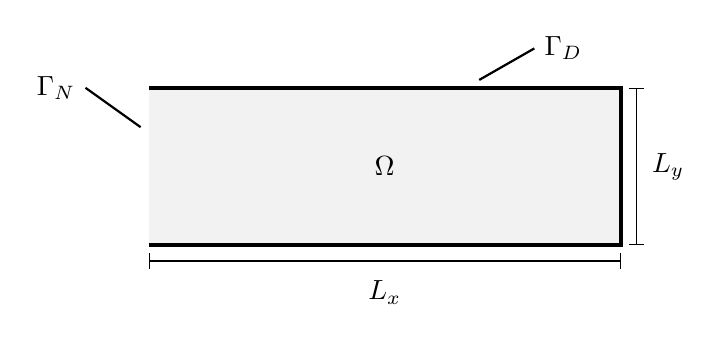
\begin{tikzpicture}
    \fill[black!5!white] (0, 0) rectangle (6, 2);
    \draw[ultra thick] (0, 0) to (6, 0) to (6, 2) to (0, 2);
    \draw[thick] (-0.8, 2) node[left] {$\Gamma_N$} to (-0.1, 1.5);
    \draw[thick] (4.9, 2.5) node[right] {$\Gamma_D$} to (4.2, 2.1);
    \draw[|-|] (0, -0.2) to (6, -0.2);
    \draw[|-|] (6.2, 0) to (6.2, 2);
    \node at (3, -0.6) {$L_x$};
    \node at (6.6, 1) {$L_y$};
    \node at (3, 1) {$\Omega$};
\end{tikzpicture}

    \caption{The rectangular resonant cavity is a medium $\Omega$ enclosed
    by a perfectly conducting boundary $\Gamma_D$ and an inlet $\Gamma_N$
    chosen to coincide with the rectangle's edge at $x=0$ for the experiments in this
    section.}
    \label{fig:rectangular_cavity}
\end{figure}

For simplicity, I set $\epsilon=\mu=1$. A uniform grid with 101 subdivisions in
the $x$- and 21 in the $y$-direction whose cells are again subdivided by their
diagonals was used to generate a mesh that allows for 4365 degrees of freedom.
The system is forced from the inlet at $x=0$ with $g_z(y) = sin(\pi y / L_y)$.

% Exploratory plots
\subsubsection{Exploration of the problem}
\label{subsubsec:exploration}

To give the reader an impression of what the solution $u_z(x, y)$ to this problem
looks like, I plot the \acrshort{FEM}-solution at the first and fifth resonant
frequency in Figures \ref{fig:rectangular-cavity-mode1} and \ref{fig:rectangular-cavity-mode5}
respectively.

\begin{figure}[ht]
    \centering
    \includegraphics{plots/rectangular_cavity_mode1.pdf}
    \caption{The solution $u_z(x, y)$ obtained with the \acrshort{FEM} at the
    first resonant frequency $\omega = 3.159$ of the cavity. Observe how at
    every perfectly conducting boundary $\Gamma_D$ (cf. Figure
    \ref{fig:rectangular_cavity}) the solution gradually goes to zero, as was imposed.}
    \label{fig:rectangular-cavity-mode1}
\end{figure}

\begin{figure}[ht]
    \centering
    \includegraphics{plots/rectangular_cavity_mode5.pdf}
    \caption{The solution $u_z(x, y)$ obtained with the \acrshort{FEM} at the
    fifth resonant frequency $\omega = 4.675$ of the cavity.}
    \label{fig:rectangular-cavity-mode5}
\end{figure}

% Rational interpolation demonstration
I now study the \acrshort{gMRI} of the quantity $||u_z||_M$ defined in
(\ref{equ:matrix-norm}). Algorithm \ref{alg:gMRI} is performed
with a tolerance of $\tau = 10^{-2}$. The candidate support points $\Omega_{\mathrm{test}}$
are 1000 uniformly spaced points in $\omega = [3, 5]$. The \acrshort{FEM} solution $u_z$
is computed and the \acrshort{gMRI} surrogate $\tilde{u}_z$ evaluated at all points in $\Omega_{\mathrm{test}}$,
and the $||.||_M$-norm for both is plotted in Figure \ref{fig:rectangular-cavity-norms}. 

\begin{figure}[ht]
    \centering
    %% Creator: Matplotlib, PGF backend
%%
%% To include the figure in your LaTeX document, write
%%   \input{<filename>.pgf}
%%
%% Make sure the required packages are loaded in your preamble
%%   \usepackage{pgf}
%%
%% Also ensure that all the required font packages are loaded; for instance,
%% the lmodern package is sometimes necessary when using math font.
%%   \usepackage{lmodern}
%%
%% Figures using additional raster images can only be included by \input if
%% they are in the same directory as the main LaTeX file. For loading figures
%% from other directories you can use the `import` package
%%   \usepackage{import}
%%
%% and then include the figures with
%%   \import{<path to file>}{<filename>.pgf}
%%
%% Matplotlib used the following preamble
%%   \usepackage{fontspec}
%%   \setmainfont{DejaVuSans.ttf}[Path=\detokenize{C:/Users/Fabio/Anaconda3/Lib/site-packages/matplotlib/mpl-data/fonts/ttf/}]
%%   \setsansfont{DejaVuSans.ttf}[Path=\detokenize{C:/Users/Fabio/Anaconda3/Lib/site-packages/matplotlib/mpl-data/fonts/ttf/}]
%%   \setmonofont{DejaVuSansMono.ttf}[Path=\detokenize{C:/Users/Fabio/Anaconda3/Lib/site-packages/matplotlib/mpl-data/fonts/ttf/}]
%%
\begingroup%
\makeatletter%
\begin{pgfpicture}%
\pgfpathrectangle{\pgfpointorigin}{\pgfqpoint{5.159353in}{3.290986in}}%
\pgfusepath{use as bounding box, clip}%
\begin{pgfscope}%
\pgfsetbuttcap%
\pgfsetmiterjoin%
\pgfsetlinewidth{0.000000pt}%
\definecolor{currentstroke}{rgb}{1.000000,1.000000,1.000000}%
\pgfsetstrokecolor{currentstroke}%
\pgfsetstrokeopacity{0.000000}%
\pgfsetdash{}{0pt}%
\pgfpathmoveto{\pgfqpoint{0.000000in}{0.000000in}}%
\pgfpathlineto{\pgfqpoint{5.159353in}{0.000000in}}%
\pgfpathlineto{\pgfqpoint{5.159353in}{3.290986in}}%
\pgfpathlineto{\pgfqpoint{0.000000in}{3.290986in}}%
\pgfpathlineto{\pgfqpoint{0.000000in}{0.000000in}}%
\pgfpathclose%
\pgfusepath{}%
\end{pgfscope}%
\begin{pgfscope}%
\pgfsetbuttcap%
\pgfsetmiterjoin%
\definecolor{currentfill}{rgb}{1.000000,1.000000,1.000000}%
\pgfsetfillcolor{currentfill}%
\pgfsetlinewidth{0.000000pt}%
\definecolor{currentstroke}{rgb}{0.000000,0.000000,0.000000}%
\pgfsetstrokecolor{currentstroke}%
\pgfsetstrokeopacity{0.000000}%
\pgfsetdash{}{0pt}%
\pgfpathmoveto{\pgfqpoint{0.622917in}{1.869736in}}%
\pgfpathlineto{\pgfqpoint{4.924167in}{1.869736in}}%
\pgfpathlineto{\pgfqpoint{4.924167in}{3.190986in}}%
\pgfpathlineto{\pgfqpoint{0.622917in}{3.190986in}}%
\pgfpathlineto{\pgfqpoint{0.622917in}{1.869736in}}%
\pgfpathclose%
\pgfusepath{fill}%
\end{pgfscope}%
\begin{pgfscope}%
\pgfsetbuttcap%
\pgfsetroundjoin%
\definecolor{currentfill}{rgb}{0.000000,0.000000,0.000000}%
\pgfsetfillcolor{currentfill}%
\pgfsetlinewidth{0.803000pt}%
\definecolor{currentstroke}{rgb}{0.000000,0.000000,0.000000}%
\pgfsetstrokecolor{currentstroke}%
\pgfsetdash{}{0pt}%
\pgfsys@defobject{currentmarker}{\pgfqpoint{0.000000in}{-0.048611in}}{\pgfqpoint{0.000000in}{0.000000in}}{%
\pgfpathmoveto{\pgfqpoint{0.000000in}{0.000000in}}%
\pgfpathlineto{\pgfqpoint{0.000000in}{-0.048611in}}%
\pgfusepath{stroke,fill}%
}%
\begin{pgfscope}%
\pgfsys@transformshift{0.622917in}{1.869736in}%
\pgfsys@useobject{currentmarker}{}%
\end{pgfscope}%
\end{pgfscope}%
\begin{pgfscope}%
\pgfsetbuttcap%
\pgfsetroundjoin%
\definecolor{currentfill}{rgb}{0.000000,0.000000,0.000000}%
\pgfsetfillcolor{currentfill}%
\pgfsetlinewidth{0.803000pt}%
\definecolor{currentstroke}{rgb}{0.000000,0.000000,0.000000}%
\pgfsetstrokecolor{currentstroke}%
\pgfsetdash{}{0pt}%
\pgfsys@defobject{currentmarker}{\pgfqpoint{0.000000in}{-0.048611in}}{\pgfqpoint{0.000000in}{0.000000in}}{%
\pgfpathmoveto{\pgfqpoint{0.000000in}{0.000000in}}%
\pgfpathlineto{\pgfqpoint{0.000000in}{-0.048611in}}%
\pgfusepath{stroke,fill}%
}%
\begin{pgfscope}%
\pgfsys@transformshift{1.160574in}{1.869736in}%
\pgfsys@useobject{currentmarker}{}%
\end{pgfscope}%
\end{pgfscope}%
\begin{pgfscope}%
\pgfsetbuttcap%
\pgfsetroundjoin%
\definecolor{currentfill}{rgb}{0.000000,0.000000,0.000000}%
\pgfsetfillcolor{currentfill}%
\pgfsetlinewidth{0.803000pt}%
\definecolor{currentstroke}{rgb}{0.000000,0.000000,0.000000}%
\pgfsetstrokecolor{currentstroke}%
\pgfsetdash{}{0pt}%
\pgfsys@defobject{currentmarker}{\pgfqpoint{0.000000in}{-0.048611in}}{\pgfqpoint{0.000000in}{0.000000in}}{%
\pgfpathmoveto{\pgfqpoint{0.000000in}{0.000000in}}%
\pgfpathlineto{\pgfqpoint{0.000000in}{-0.048611in}}%
\pgfusepath{stroke,fill}%
}%
\begin{pgfscope}%
\pgfsys@transformshift{1.698230in}{1.869736in}%
\pgfsys@useobject{currentmarker}{}%
\end{pgfscope}%
\end{pgfscope}%
\begin{pgfscope}%
\pgfsetbuttcap%
\pgfsetroundjoin%
\definecolor{currentfill}{rgb}{0.000000,0.000000,0.000000}%
\pgfsetfillcolor{currentfill}%
\pgfsetlinewidth{0.803000pt}%
\definecolor{currentstroke}{rgb}{0.000000,0.000000,0.000000}%
\pgfsetstrokecolor{currentstroke}%
\pgfsetdash{}{0pt}%
\pgfsys@defobject{currentmarker}{\pgfqpoint{0.000000in}{-0.048611in}}{\pgfqpoint{0.000000in}{0.000000in}}{%
\pgfpathmoveto{\pgfqpoint{0.000000in}{0.000000in}}%
\pgfpathlineto{\pgfqpoint{0.000000in}{-0.048611in}}%
\pgfusepath{stroke,fill}%
}%
\begin{pgfscope}%
\pgfsys@transformshift{2.235886in}{1.869736in}%
\pgfsys@useobject{currentmarker}{}%
\end{pgfscope}%
\end{pgfscope}%
\begin{pgfscope}%
\pgfsetbuttcap%
\pgfsetroundjoin%
\definecolor{currentfill}{rgb}{0.000000,0.000000,0.000000}%
\pgfsetfillcolor{currentfill}%
\pgfsetlinewidth{0.803000pt}%
\definecolor{currentstroke}{rgb}{0.000000,0.000000,0.000000}%
\pgfsetstrokecolor{currentstroke}%
\pgfsetdash{}{0pt}%
\pgfsys@defobject{currentmarker}{\pgfqpoint{0.000000in}{-0.048611in}}{\pgfqpoint{0.000000in}{0.000000in}}{%
\pgfpathmoveto{\pgfqpoint{0.000000in}{0.000000in}}%
\pgfpathlineto{\pgfqpoint{0.000000in}{-0.048611in}}%
\pgfusepath{stroke,fill}%
}%
\begin{pgfscope}%
\pgfsys@transformshift{2.773543in}{1.869736in}%
\pgfsys@useobject{currentmarker}{}%
\end{pgfscope}%
\end{pgfscope}%
\begin{pgfscope}%
\pgfsetbuttcap%
\pgfsetroundjoin%
\definecolor{currentfill}{rgb}{0.000000,0.000000,0.000000}%
\pgfsetfillcolor{currentfill}%
\pgfsetlinewidth{0.803000pt}%
\definecolor{currentstroke}{rgb}{0.000000,0.000000,0.000000}%
\pgfsetstrokecolor{currentstroke}%
\pgfsetdash{}{0pt}%
\pgfsys@defobject{currentmarker}{\pgfqpoint{0.000000in}{-0.048611in}}{\pgfqpoint{0.000000in}{0.000000in}}{%
\pgfpathmoveto{\pgfqpoint{0.000000in}{0.000000in}}%
\pgfpathlineto{\pgfqpoint{0.000000in}{-0.048611in}}%
\pgfusepath{stroke,fill}%
}%
\begin{pgfscope}%
\pgfsys@transformshift{3.311199in}{1.869736in}%
\pgfsys@useobject{currentmarker}{}%
\end{pgfscope}%
\end{pgfscope}%
\begin{pgfscope}%
\pgfsetbuttcap%
\pgfsetroundjoin%
\definecolor{currentfill}{rgb}{0.000000,0.000000,0.000000}%
\pgfsetfillcolor{currentfill}%
\pgfsetlinewidth{0.803000pt}%
\definecolor{currentstroke}{rgb}{0.000000,0.000000,0.000000}%
\pgfsetstrokecolor{currentstroke}%
\pgfsetdash{}{0pt}%
\pgfsys@defobject{currentmarker}{\pgfqpoint{0.000000in}{-0.048611in}}{\pgfqpoint{0.000000in}{0.000000in}}{%
\pgfpathmoveto{\pgfqpoint{0.000000in}{0.000000in}}%
\pgfpathlineto{\pgfqpoint{0.000000in}{-0.048611in}}%
\pgfusepath{stroke,fill}%
}%
\begin{pgfscope}%
\pgfsys@transformshift{3.848855in}{1.869736in}%
\pgfsys@useobject{currentmarker}{}%
\end{pgfscope}%
\end{pgfscope}%
\begin{pgfscope}%
\pgfsetbuttcap%
\pgfsetroundjoin%
\definecolor{currentfill}{rgb}{0.000000,0.000000,0.000000}%
\pgfsetfillcolor{currentfill}%
\pgfsetlinewidth{0.803000pt}%
\definecolor{currentstroke}{rgb}{0.000000,0.000000,0.000000}%
\pgfsetstrokecolor{currentstroke}%
\pgfsetdash{}{0pt}%
\pgfsys@defobject{currentmarker}{\pgfqpoint{0.000000in}{-0.048611in}}{\pgfqpoint{0.000000in}{0.000000in}}{%
\pgfpathmoveto{\pgfqpoint{0.000000in}{0.000000in}}%
\pgfpathlineto{\pgfqpoint{0.000000in}{-0.048611in}}%
\pgfusepath{stroke,fill}%
}%
\begin{pgfscope}%
\pgfsys@transformshift{4.386511in}{1.869736in}%
\pgfsys@useobject{currentmarker}{}%
\end{pgfscope}%
\end{pgfscope}%
\begin{pgfscope}%
\pgfsetbuttcap%
\pgfsetroundjoin%
\definecolor{currentfill}{rgb}{0.000000,0.000000,0.000000}%
\pgfsetfillcolor{currentfill}%
\pgfsetlinewidth{0.803000pt}%
\definecolor{currentstroke}{rgb}{0.000000,0.000000,0.000000}%
\pgfsetstrokecolor{currentstroke}%
\pgfsetdash{}{0pt}%
\pgfsys@defobject{currentmarker}{\pgfqpoint{0.000000in}{-0.048611in}}{\pgfqpoint{0.000000in}{0.000000in}}{%
\pgfpathmoveto{\pgfqpoint{0.000000in}{0.000000in}}%
\pgfpathlineto{\pgfqpoint{0.000000in}{-0.048611in}}%
\pgfusepath{stroke,fill}%
}%
\begin{pgfscope}%
\pgfsys@transformshift{4.924168in}{1.869736in}%
\pgfsys@useobject{currentmarker}{}%
\end{pgfscope}%
\end{pgfscope}%
\begin{pgfscope}%
\pgfpathrectangle{\pgfqpoint{0.622917in}{1.869736in}}{\pgfqpoint{4.301250in}{1.321250in}}%
\pgfusepath{clip}%
\pgfsetrectcap%
\pgfsetroundjoin%
\pgfsetlinewidth{0.803000pt}%
\definecolor{currentstroke}{rgb}{0.690196,0.690196,0.690196}%
\pgfsetstrokecolor{currentstroke}%
\pgfsetdash{}{0pt}%
\pgfpathmoveto{\pgfqpoint{0.622917in}{2.430927in}}%
\pgfpathlineto{\pgfqpoint{4.924167in}{2.430927in}}%
\pgfusepath{stroke}%
\end{pgfscope}%
\begin{pgfscope}%
\pgfsetbuttcap%
\pgfsetroundjoin%
\definecolor{currentfill}{rgb}{0.000000,0.000000,0.000000}%
\pgfsetfillcolor{currentfill}%
\pgfsetlinewidth{0.803000pt}%
\definecolor{currentstroke}{rgb}{0.000000,0.000000,0.000000}%
\pgfsetstrokecolor{currentstroke}%
\pgfsetdash{}{0pt}%
\pgfsys@defobject{currentmarker}{\pgfqpoint{-0.048611in}{0.000000in}}{\pgfqpoint{-0.000000in}{0.000000in}}{%
\pgfpathmoveto{\pgfqpoint{-0.000000in}{0.000000in}}%
\pgfpathlineto{\pgfqpoint{-0.048611in}{0.000000in}}%
\pgfusepath{stroke,fill}%
}%
\begin{pgfscope}%
\pgfsys@transformshift{0.622917in}{2.430927in}%
\pgfsys@useobject{currentmarker}{}%
\end{pgfscope}%
\end{pgfscope}%
\begin{pgfscope}%
\definecolor{textcolor}{rgb}{0.000000,0.000000,0.000000}%
\pgfsetstrokecolor{textcolor}%
\pgfsetfillcolor{textcolor}%
\pgftext[x=0.307639in, y=2.372889in, left, base]{\color{textcolor}\rmfamily\fontsize{11.000000}{13.200000}\selectfont \(\displaystyle {10^{1}}\)}%
\end{pgfscope}%
\begin{pgfscope}%
\pgfpathrectangle{\pgfqpoint{0.622917in}{1.869736in}}{\pgfqpoint{4.301250in}{1.321250in}}%
\pgfusepath{clip}%
\pgfsetrectcap%
\pgfsetroundjoin%
\pgfsetlinewidth{0.803000pt}%
\definecolor{currentstroke}{rgb}{0.690196,0.690196,0.690196}%
\pgfsetstrokecolor{currentstroke}%
\pgfsetdash{}{0pt}%
\pgfpathmoveto{\pgfqpoint{0.622917in}{3.091552in}}%
\pgfpathlineto{\pgfqpoint{4.924167in}{3.091552in}}%
\pgfusepath{stroke}%
\end{pgfscope}%
\begin{pgfscope}%
\pgfsetbuttcap%
\pgfsetroundjoin%
\definecolor{currentfill}{rgb}{0.000000,0.000000,0.000000}%
\pgfsetfillcolor{currentfill}%
\pgfsetlinewidth{0.803000pt}%
\definecolor{currentstroke}{rgb}{0.000000,0.000000,0.000000}%
\pgfsetstrokecolor{currentstroke}%
\pgfsetdash{}{0pt}%
\pgfsys@defobject{currentmarker}{\pgfqpoint{-0.048611in}{0.000000in}}{\pgfqpoint{-0.000000in}{0.000000in}}{%
\pgfpathmoveto{\pgfqpoint{-0.000000in}{0.000000in}}%
\pgfpathlineto{\pgfqpoint{-0.048611in}{0.000000in}}%
\pgfusepath{stroke,fill}%
}%
\begin{pgfscope}%
\pgfsys@transformshift{0.622917in}{3.091552in}%
\pgfsys@useobject{currentmarker}{}%
\end{pgfscope}%
\end{pgfscope}%
\begin{pgfscope}%
\definecolor{textcolor}{rgb}{0.000000,0.000000,0.000000}%
\pgfsetstrokecolor{textcolor}%
\pgfsetfillcolor{textcolor}%
\pgftext[x=0.307639in, y=3.033514in, left, base]{\color{textcolor}\rmfamily\fontsize{11.000000}{13.200000}\selectfont \(\displaystyle {10^{3}}\)}%
\end{pgfscope}%
\begin{pgfscope}%
\definecolor{textcolor}{rgb}{0.000000,0.000000,0.000000}%
\pgfsetstrokecolor{textcolor}%
\pgfsetfillcolor{textcolor}%
\pgftext[x=0.252083in,y=2.530361in,,bottom,rotate=90.000000]{\color{textcolor}\rmfamily\fontsize{11.000000}{13.200000}\selectfont \(\displaystyle ||u_z(\omega)||_M\)}%
\end{pgfscope}%
\begin{pgfscope}%
\pgfpathrectangle{\pgfqpoint{0.622917in}{1.869736in}}{\pgfqpoint{4.301250in}{1.321250in}}%
\pgfusepath{clip}%
\pgfsetrectcap%
\pgfsetroundjoin%
\pgfsetlinewidth{1.505625pt}%
\definecolor{currentstroke}{rgb}{0.001462,0.000466,0.013866}%
\pgfsetstrokecolor{currentstroke}%
\pgfsetdash{}{0pt}%
\pgfpathmoveto{\pgfqpoint{0.622917in}{2.014294in}}%
\pgfpathlineto{\pgfqpoint{0.674584in}{2.033451in}}%
\pgfpathlineto{\pgfqpoint{0.717640in}{2.052591in}}%
\pgfpathlineto{\pgfqpoint{0.756390in}{2.073322in}}%
\pgfpathlineto{\pgfqpoint{0.786529in}{2.092683in}}%
\pgfpathlineto{\pgfqpoint{0.812362in}{2.112441in}}%
\pgfpathlineto{\pgfqpoint{0.838195in}{2.136317in}}%
\pgfpathlineto{\pgfqpoint{0.859723in}{2.160729in}}%
\pgfpathlineto{\pgfqpoint{0.876945in}{2.184553in}}%
\pgfpathlineto{\pgfqpoint{0.894168in}{2.214016in}}%
\pgfpathlineto{\pgfqpoint{0.907084in}{2.241622in}}%
\pgfpathlineto{\pgfqpoint{0.920001in}{2.276585in}}%
\pgfpathlineto{\pgfqpoint{0.932917in}{2.323884in}}%
\pgfpathlineto{\pgfqpoint{0.941529in}{2.367804in}}%
\pgfpathlineto{\pgfqpoint{0.950140in}{2.432100in}}%
\pgfpathlineto{\pgfqpoint{0.954445in}{2.480059in}}%
\pgfpathlineto{\pgfqpoint{0.958751in}{2.552865in}}%
\pgfpathlineto{\pgfqpoint{0.963056in}{2.708641in}}%
\pgfpathlineto{\pgfqpoint{0.967362in}{2.713871in}}%
\pgfpathlineto{\pgfqpoint{0.971668in}{2.554490in}}%
\pgfpathlineto{\pgfqpoint{0.980279in}{2.432586in}}%
\pgfpathlineto{\pgfqpoint{0.988890in}{2.367989in}}%
\pgfpathlineto{\pgfqpoint{0.997501in}{2.324084in}}%
\pgfpathlineto{\pgfqpoint{1.010418in}{2.277359in}}%
\pgfpathlineto{\pgfqpoint{1.023334in}{2.243779in}}%
\pgfpathlineto{\pgfqpoint{1.036251in}{2.218597in}}%
\pgfpathlineto{\pgfqpoint{1.049168in}{2.199609in}}%
\pgfpathlineto{\pgfqpoint{1.062084in}{2.185692in}}%
\pgfpathlineto{\pgfqpoint{1.075001in}{2.176257in}}%
\pgfpathlineto{\pgfqpoint{1.087918in}{2.171005in}}%
\pgfpathlineto{\pgfqpoint{1.100834in}{2.169807in}}%
\pgfpathlineto{\pgfqpoint{1.113751in}{2.172642in}}%
\pgfpathlineto{\pgfqpoint{1.126667in}{2.179597in}}%
\pgfpathlineto{\pgfqpoint{1.139584in}{2.190894in}}%
\pgfpathlineto{\pgfqpoint{1.152501in}{2.206981in}}%
\pgfpathlineto{\pgfqpoint{1.165418in}{2.228716in}}%
\pgfpathlineto{\pgfqpoint{1.178334in}{2.257742in}}%
\pgfpathlineto{\pgfqpoint{1.191251in}{2.297415in}}%
\pgfpathlineto{\pgfqpoint{1.199862in}{2.333304in}}%
\pgfpathlineto{\pgfqpoint{1.208473in}{2.382550in}}%
\pgfpathlineto{\pgfqpoint{1.217084in}{2.459587in}}%
\pgfpathlineto{\pgfqpoint{1.221390in}{2.523137in}}%
\pgfpathlineto{\pgfqpoint{1.225695in}{2.640549in}}%
\pgfpathlineto{\pgfqpoint{1.230001in}{2.828938in}}%
\pgfpathlineto{\pgfqpoint{1.234306in}{2.578759in}}%
\pgfpathlineto{\pgfqpoint{1.238612in}{2.492488in}}%
\pgfpathlineto{\pgfqpoint{1.247223in}{2.400310in}}%
\pgfpathlineto{\pgfqpoint{1.255834in}{2.344949in}}%
\pgfpathlineto{\pgfqpoint{1.264445in}{2.305433in}}%
\pgfpathlineto{\pgfqpoint{1.277362in}{2.261796in}}%
\pgfpathlineto{\pgfqpoint{1.290279in}{2.229085in}}%
\pgfpathlineto{\pgfqpoint{1.307501in}{2.195634in}}%
\pgfpathlineto{\pgfqpoint{1.324723in}{2.169701in}}%
\pgfpathlineto{\pgfqpoint{1.341945in}{2.148928in}}%
\pgfpathlineto{\pgfqpoint{1.363473in}{2.128254in}}%
\pgfpathlineto{\pgfqpoint{1.385001in}{2.112108in}}%
\pgfpathlineto{\pgfqpoint{1.406529in}{2.099639in}}%
\pgfpathlineto{\pgfqpoint{1.428056in}{2.090358in}}%
\pgfpathlineto{\pgfqpoint{1.449584in}{2.084000in}}%
\pgfpathlineto{\pgfqpoint{1.471112in}{2.080443in}}%
\pgfpathlineto{\pgfqpoint{1.492640in}{2.079674in}}%
\pgfpathlineto{\pgfqpoint{1.514168in}{2.081762in}}%
\pgfpathlineto{\pgfqpoint{1.535695in}{2.086860in}}%
\pgfpathlineto{\pgfqpoint{1.557223in}{2.095214in}}%
\pgfpathlineto{\pgfqpoint{1.578751in}{2.107207in}}%
\pgfpathlineto{\pgfqpoint{1.600279in}{2.123437in}}%
\pgfpathlineto{\pgfqpoint{1.617501in}{2.140108in}}%
\pgfpathlineto{\pgfqpoint{1.634723in}{2.160912in}}%
\pgfpathlineto{\pgfqpoint{1.651945in}{2.187180in}}%
\pgfpathlineto{\pgfqpoint{1.664862in}{2.211839in}}%
\pgfpathlineto{\pgfqpoint{1.677779in}{2.242674in}}%
\pgfpathlineto{\pgfqpoint{1.690695in}{2.283083in}}%
\pgfpathlineto{\pgfqpoint{1.699306in}{2.318751in}}%
\pgfpathlineto{\pgfqpoint{1.707917in}{2.366827in}}%
\pgfpathlineto{\pgfqpoint{1.716529in}{2.440270in}}%
\pgfpathlineto{\pgfqpoint{1.720834in}{2.498885in}}%
\pgfpathlineto{\pgfqpoint{1.725140in}{2.599905in}}%
\pgfpathlineto{\pgfqpoint{1.729445in}{3.139147in}}%
\pgfpathlineto{\pgfqpoint{1.733751in}{2.593291in}}%
\pgfpathlineto{\pgfqpoint{1.738056in}{2.495456in}}%
\pgfpathlineto{\pgfqpoint{1.746668in}{2.396884in}}%
\pgfpathlineto{\pgfqpoint{1.755279in}{2.339127in}}%
\pgfpathlineto{\pgfqpoint{1.763890in}{2.298211in}}%
\pgfpathlineto{\pgfqpoint{1.776806in}{2.253109in}}%
\pgfpathlineto{\pgfqpoint{1.789723in}{2.219213in}}%
\pgfpathlineto{\pgfqpoint{1.806945in}{2.184303in}}%
\pgfpathlineto{\pgfqpoint{1.824167in}{2.156904in}}%
\pgfpathlineto{\pgfqpoint{1.841390in}{2.134574in}}%
\pgfpathlineto{\pgfqpoint{1.862917in}{2.111730in}}%
\pgfpathlineto{\pgfqpoint{1.884445in}{2.093055in}}%
\pgfpathlineto{\pgfqpoint{1.910279in}{2.074800in}}%
\pgfpathlineto{\pgfqpoint{1.936112in}{2.060113in}}%
\pgfpathlineto{\pgfqpoint{1.966251in}{2.046638in}}%
\pgfpathlineto{\pgfqpoint{1.996390in}{2.036517in}}%
\pgfpathlineto{\pgfqpoint{2.026529in}{2.029386in}}%
\pgfpathlineto{\pgfqpoint{2.056668in}{2.025057in}}%
\pgfpathlineto{\pgfqpoint{2.086806in}{2.023469in}}%
\pgfpathlineto{\pgfqpoint{2.116945in}{2.024662in}}%
\pgfpathlineto{\pgfqpoint{2.147084in}{2.028769in}}%
\pgfpathlineto{\pgfqpoint{2.177223in}{2.036028in}}%
\pgfpathlineto{\pgfqpoint{2.207362in}{2.046810in}}%
\pgfpathlineto{\pgfqpoint{2.233195in}{2.059284in}}%
\pgfpathlineto{\pgfqpoint{2.259029in}{2.075318in}}%
\pgfpathlineto{\pgfqpoint{2.280556in}{2.092009in}}%
\pgfpathlineto{\pgfqpoint{2.302084in}{2.112544in}}%
\pgfpathlineto{\pgfqpoint{2.319306in}{2.132562in}}%
\pgfpathlineto{\pgfqpoint{2.336529in}{2.156875in}}%
\pgfpathlineto{\pgfqpoint{2.353751in}{2.187234in}}%
\pgfpathlineto{\pgfqpoint{2.366668in}{2.215839in}}%
\pgfpathlineto{\pgfqpoint{2.379584in}{2.252224in}}%
\pgfpathlineto{\pgfqpoint{2.388195in}{2.283235in}}%
\pgfpathlineto{\pgfqpoint{2.396806in}{2.323145in}}%
\pgfpathlineto{\pgfqpoint{2.405417in}{2.378966in}}%
\pgfpathlineto{\pgfqpoint{2.409723in}{2.418058in}}%
\pgfpathlineto{\pgfqpoint{2.414029in}{2.472065in}}%
\pgfpathlineto{\pgfqpoint{2.418334in}{2.559846in}}%
\pgfpathlineto{\pgfqpoint{2.422640in}{2.827014in}}%
\pgfpathlineto{\pgfqpoint{2.426945in}{2.613099in}}%
\pgfpathlineto{\pgfqpoint{2.431251in}{2.498343in}}%
\pgfpathlineto{\pgfqpoint{2.439862in}{2.391833in}}%
\pgfpathlineto{\pgfqpoint{2.448473in}{2.331442in}}%
\pgfpathlineto{\pgfqpoint{2.457084in}{2.289156in}}%
\pgfpathlineto{\pgfqpoint{2.470001in}{2.242821in}}%
\pgfpathlineto{\pgfqpoint{2.482918in}{2.208082in}}%
\pgfpathlineto{\pgfqpoint{2.500140in}{2.172282in}}%
\pgfpathlineto{\pgfqpoint{2.517362in}{2.144092in}}%
\pgfpathlineto{\pgfqpoint{2.538890in}{2.115831in}}%
\pgfpathlineto{\pgfqpoint{2.560417in}{2.092928in}}%
\pgfpathlineto{\pgfqpoint{2.586251in}{2.070462in}}%
\pgfpathlineto{\pgfqpoint{2.612084in}{2.052057in}}%
\pgfpathlineto{\pgfqpoint{2.642223in}{2.034492in}}%
\pgfpathlineto{\pgfqpoint{2.676667in}{2.018462in}}%
\pgfpathlineto{\pgfqpoint{2.711112in}{2.005936in}}%
\pgfpathlineto{\pgfqpoint{2.749862in}{1.995381in}}%
\pgfpathlineto{\pgfqpoint{2.788612in}{1.988152in}}%
\pgfpathlineto{\pgfqpoint{2.827362in}{1.984023in}}%
\pgfpathlineto{\pgfqpoint{2.866112in}{1.982924in}}%
\pgfpathlineto{\pgfqpoint{2.904862in}{1.984911in}}%
\pgfpathlineto{\pgfqpoint{2.943612in}{1.990166in}}%
\pgfpathlineto{\pgfqpoint{2.978056in}{1.997839in}}%
\pgfpathlineto{\pgfqpoint{3.012501in}{2.008704in}}%
\pgfpathlineto{\pgfqpoint{3.042640in}{2.021247in}}%
\pgfpathlineto{\pgfqpoint{3.072779in}{2.037186in}}%
\pgfpathlineto{\pgfqpoint{3.098612in}{2.054178in}}%
\pgfpathlineto{\pgfqpoint{3.124445in}{2.075098in}}%
\pgfpathlineto{\pgfqpoint{3.145973in}{2.096472in}}%
\pgfpathlineto{\pgfqpoint{3.167501in}{2.122758in}}%
\pgfpathlineto{\pgfqpoint{3.184723in}{2.148762in}}%
\pgfpathlineto{\pgfqpoint{3.201945in}{2.181318in}}%
\pgfpathlineto{\pgfqpoint{3.214862in}{2.212249in}}%
\pgfpathlineto{\pgfqpoint{3.227779in}{2.252205in}}%
\pgfpathlineto{\pgfqpoint{3.236390in}{2.287036in}}%
\pgfpathlineto{\pgfqpoint{3.245001in}{2.333367in}}%
\pgfpathlineto{\pgfqpoint{3.253612in}{2.402520in}}%
\pgfpathlineto{\pgfqpoint{3.257918in}{2.455812in}}%
\pgfpathlineto{\pgfqpoint{3.262223in}{2.541661in}}%
\pgfpathlineto{\pgfqpoint{3.266529in}{2.787579in}}%
\pgfpathlineto{\pgfqpoint{3.275140in}{2.487293in}}%
\pgfpathlineto{\pgfqpoint{3.283751in}{2.379265in}}%
\pgfpathlineto{\pgfqpoint{3.292362in}{2.318380in}}%
\pgfpathlineto{\pgfqpoint{3.300973in}{2.275827in}}%
\pgfpathlineto{\pgfqpoint{3.313890in}{2.229225in}}%
\pgfpathlineto{\pgfqpoint{3.326806in}{2.194274in}}%
\pgfpathlineto{\pgfqpoint{3.344029in}{2.158208in}}%
\pgfpathlineto{\pgfqpoint{3.361251in}{2.129742in}}%
\pgfpathlineto{\pgfqpoint{3.382779in}{2.101106in}}%
\pgfpathlineto{\pgfqpoint{3.404306in}{2.077786in}}%
\pgfpathlineto{\pgfqpoint{3.430140in}{2.054755in}}%
\pgfpathlineto{\pgfqpoint{3.455973in}{2.035710in}}%
\pgfpathlineto{\pgfqpoint{3.486112in}{2.017293in}}%
\pgfpathlineto{\pgfqpoint{3.520556in}{2.000129in}}%
\pgfpathlineto{\pgfqpoint{3.555001in}{1.986264in}}%
\pgfpathlineto{\pgfqpoint{3.593751in}{1.973906in}}%
\pgfpathlineto{\pgfqpoint{3.636806in}{1.963608in}}%
\pgfpathlineto{\pgfqpoint{3.679862in}{1.956514in}}%
\pgfpathlineto{\pgfqpoint{3.722917in}{1.952399in}}%
\pgfpathlineto{\pgfqpoint{3.765973in}{1.951180in}}%
\pgfpathlineto{\pgfqpoint{3.809029in}{1.952897in}}%
\pgfpathlineto{\pgfqpoint{3.852084in}{1.957705in}}%
\pgfpathlineto{\pgfqpoint{3.890834in}{1.964908in}}%
\pgfpathlineto{\pgfqpoint{3.929584in}{1.975175in}}%
\pgfpathlineto{\pgfqpoint{3.964029in}{1.987272in}}%
\pgfpathlineto{\pgfqpoint{3.998473in}{2.002707in}}%
\pgfpathlineto{\pgfqpoint{4.028612in}{2.019576in}}%
\pgfpathlineto{\pgfqpoint{4.054445in}{2.037182in}}%
\pgfpathlineto{\pgfqpoint{4.080279in}{2.058548in}}%
\pgfpathlineto{\pgfqpoint{4.101806in}{2.080153in}}%
\pgfpathlineto{\pgfqpoint{4.123334in}{2.106520in}}%
\pgfpathlineto{\pgfqpoint{4.140556in}{2.132448in}}%
\pgfpathlineto{\pgfqpoint{4.157779in}{2.164738in}}%
\pgfpathlineto{\pgfqpoint{4.170695in}{2.195262in}}%
\pgfpathlineto{\pgfqpoint{4.183612in}{2.234467in}}%
\pgfpathlineto{\pgfqpoint{4.192223in}{2.268413in}}%
\pgfpathlineto{\pgfqpoint{4.200834in}{2.313157in}}%
\pgfpathlineto{\pgfqpoint{4.209445in}{2.378774in}}%
\pgfpathlineto{\pgfqpoint{4.213751in}{2.428002in}}%
\pgfpathlineto{\pgfqpoint{4.218056in}{2.503634in}}%
\pgfpathlineto{\pgfqpoint{4.222362in}{2.673836in}}%
\pgfpathlineto{\pgfqpoint{4.226667in}{2.638800in}}%
\pgfpathlineto{\pgfqpoint{4.230973in}{2.491926in}}%
\pgfpathlineto{\pgfqpoint{4.239584in}{2.373585in}}%
\pgfpathlineto{\pgfqpoint{4.248195in}{2.309655in}}%
\pgfpathlineto{\pgfqpoint{4.256806in}{2.265631in}}%
\pgfpathlineto{\pgfqpoint{4.269723in}{2.217829in}}%
\pgfpathlineto{\pgfqpoint{4.282640in}{2.182171in}}%
\pgfpathlineto{\pgfqpoint{4.299862in}{2.145484in}}%
\pgfpathlineto{\pgfqpoint{4.317084in}{2.116567in}}%
\pgfpathlineto{\pgfqpoint{4.338612in}{2.087475in}}%
\pgfpathlineto{\pgfqpoint{4.360140in}{2.063753in}}%
\pgfpathlineto{\pgfqpoint{4.385973in}{2.040263in}}%
\pgfpathlineto{\pgfqpoint{4.411806in}{2.020758in}}%
\pgfpathlineto{\pgfqpoint{4.441945in}{2.001778in}}%
\pgfpathlineto{\pgfqpoint{4.476390in}{1.983915in}}%
\pgfpathlineto{\pgfqpoint{4.515140in}{1.967635in}}%
\pgfpathlineto{\pgfqpoint{4.553890in}{1.954611in}}%
\pgfpathlineto{\pgfqpoint{4.596945in}{1.943323in}}%
\pgfpathlineto{\pgfqpoint{4.644306in}{1.934261in}}%
\pgfpathlineto{\pgfqpoint{4.691668in}{1.928369in}}%
\pgfpathlineto{\pgfqpoint{4.739029in}{1.925470in}}%
\pgfpathlineto{\pgfqpoint{4.786390in}{1.925526in}}%
\pgfpathlineto{\pgfqpoint{4.833751in}{1.928621in}}%
\pgfpathlineto{\pgfqpoint{4.881112in}{1.934967in}}%
\pgfpathlineto{\pgfqpoint{4.924168in}{1.943862in}}%
\pgfpathlineto{\pgfqpoint{4.924168in}{1.943862in}}%
\pgfusepath{stroke}%
\end{pgfscope}%
\begin{pgfscope}%
\pgfsetrectcap%
\pgfsetmiterjoin%
\pgfsetlinewidth{0.803000pt}%
\definecolor{currentstroke}{rgb}{0.000000,0.000000,0.000000}%
\pgfsetstrokecolor{currentstroke}%
\pgfsetdash{}{0pt}%
\pgfpathmoveto{\pgfqpoint{0.622917in}{1.869736in}}%
\pgfpathlineto{\pgfqpoint{0.622917in}{3.190986in}}%
\pgfusepath{stroke}%
\end{pgfscope}%
\begin{pgfscope}%
\pgfsetrectcap%
\pgfsetmiterjoin%
\pgfsetlinewidth{0.803000pt}%
\definecolor{currentstroke}{rgb}{0.000000,0.000000,0.000000}%
\pgfsetstrokecolor{currentstroke}%
\pgfsetdash{}{0pt}%
\pgfpathmoveto{\pgfqpoint{4.924167in}{1.869736in}}%
\pgfpathlineto{\pgfqpoint{4.924167in}{3.190986in}}%
\pgfusepath{stroke}%
\end{pgfscope}%
\begin{pgfscope}%
\pgfsetrectcap%
\pgfsetmiterjoin%
\pgfsetlinewidth{0.803000pt}%
\definecolor{currentstroke}{rgb}{0.000000,0.000000,0.000000}%
\pgfsetstrokecolor{currentstroke}%
\pgfsetdash{}{0pt}%
\pgfpathmoveto{\pgfqpoint{0.622917in}{1.869736in}}%
\pgfpathlineto{\pgfqpoint{4.924168in}{1.869736in}}%
\pgfusepath{stroke}%
\end{pgfscope}%
\begin{pgfscope}%
\pgfsetrectcap%
\pgfsetmiterjoin%
\pgfsetlinewidth{0.803000pt}%
\definecolor{currentstroke}{rgb}{0.000000,0.000000,0.000000}%
\pgfsetstrokecolor{currentstroke}%
\pgfsetdash{}{0pt}%
\pgfpathmoveto{\pgfqpoint{0.622917in}{3.190986in}}%
\pgfpathlineto{\pgfqpoint{4.924168in}{3.190986in}}%
\pgfusepath{stroke}%
\end{pgfscope}%
\begin{pgfscope}%
\pgfsetbuttcap%
\pgfsetmiterjoin%
\definecolor{currentfill}{rgb}{1.000000,1.000000,1.000000}%
\pgfsetfillcolor{currentfill}%
\pgfsetlinewidth{0.000000pt}%
\definecolor{currentstroke}{rgb}{0.000000,0.000000,0.000000}%
\pgfsetstrokecolor{currentstroke}%
\pgfsetstrokeopacity{0.000000}%
\pgfsetdash{}{0pt}%
\pgfpathmoveto{\pgfqpoint{0.622917in}{0.548486in}}%
\pgfpathlineto{\pgfqpoint{4.924167in}{0.548486in}}%
\pgfpathlineto{\pgfqpoint{4.924167in}{1.869736in}}%
\pgfpathlineto{\pgfqpoint{0.622917in}{1.869736in}}%
\pgfpathlineto{\pgfqpoint{0.622917in}{0.548486in}}%
\pgfpathclose%
\pgfusepath{fill}%
\end{pgfscope}%
\begin{pgfscope}%
\pgfsetbuttcap%
\pgfsetroundjoin%
\definecolor{currentfill}{rgb}{0.000000,0.000000,0.000000}%
\pgfsetfillcolor{currentfill}%
\pgfsetlinewidth{0.803000pt}%
\definecolor{currentstroke}{rgb}{0.000000,0.000000,0.000000}%
\pgfsetstrokecolor{currentstroke}%
\pgfsetdash{}{0pt}%
\pgfsys@defobject{currentmarker}{\pgfqpoint{0.000000in}{-0.048611in}}{\pgfqpoint{0.000000in}{0.000000in}}{%
\pgfpathmoveto{\pgfqpoint{0.000000in}{0.000000in}}%
\pgfpathlineto{\pgfqpoint{0.000000in}{-0.048611in}}%
\pgfusepath{stroke,fill}%
}%
\begin{pgfscope}%
\pgfsys@transformshift{0.622917in}{0.548486in}%
\pgfsys@useobject{currentmarker}{}%
\end{pgfscope}%
\end{pgfscope}%
\begin{pgfscope}%
\definecolor{textcolor}{rgb}{0.000000,0.000000,0.000000}%
\pgfsetstrokecolor{textcolor}%
\pgfsetfillcolor{textcolor}%
\pgftext[x=0.622917in,y=0.451264in,,top]{\color{textcolor}\rmfamily\fontsize{11.000000}{13.200000}\selectfont \(\displaystyle {3.00}\)}%
\end{pgfscope}%
\begin{pgfscope}%
\pgfsetbuttcap%
\pgfsetroundjoin%
\definecolor{currentfill}{rgb}{0.000000,0.000000,0.000000}%
\pgfsetfillcolor{currentfill}%
\pgfsetlinewidth{0.803000pt}%
\definecolor{currentstroke}{rgb}{0.000000,0.000000,0.000000}%
\pgfsetstrokecolor{currentstroke}%
\pgfsetdash{}{0pt}%
\pgfsys@defobject{currentmarker}{\pgfqpoint{0.000000in}{-0.048611in}}{\pgfqpoint{0.000000in}{0.000000in}}{%
\pgfpathmoveto{\pgfqpoint{0.000000in}{0.000000in}}%
\pgfpathlineto{\pgfqpoint{0.000000in}{-0.048611in}}%
\pgfusepath{stroke,fill}%
}%
\begin{pgfscope}%
\pgfsys@transformshift{1.160574in}{0.548486in}%
\pgfsys@useobject{currentmarker}{}%
\end{pgfscope}%
\end{pgfscope}%
\begin{pgfscope}%
\definecolor{textcolor}{rgb}{0.000000,0.000000,0.000000}%
\pgfsetstrokecolor{textcolor}%
\pgfsetfillcolor{textcolor}%
\pgftext[x=1.160574in,y=0.451264in,,top]{\color{textcolor}\rmfamily\fontsize{11.000000}{13.200000}\selectfont \(\displaystyle {3.25}\)}%
\end{pgfscope}%
\begin{pgfscope}%
\pgfsetbuttcap%
\pgfsetroundjoin%
\definecolor{currentfill}{rgb}{0.000000,0.000000,0.000000}%
\pgfsetfillcolor{currentfill}%
\pgfsetlinewidth{0.803000pt}%
\definecolor{currentstroke}{rgb}{0.000000,0.000000,0.000000}%
\pgfsetstrokecolor{currentstroke}%
\pgfsetdash{}{0pt}%
\pgfsys@defobject{currentmarker}{\pgfqpoint{0.000000in}{-0.048611in}}{\pgfqpoint{0.000000in}{0.000000in}}{%
\pgfpathmoveto{\pgfqpoint{0.000000in}{0.000000in}}%
\pgfpathlineto{\pgfqpoint{0.000000in}{-0.048611in}}%
\pgfusepath{stroke,fill}%
}%
\begin{pgfscope}%
\pgfsys@transformshift{1.698230in}{0.548486in}%
\pgfsys@useobject{currentmarker}{}%
\end{pgfscope}%
\end{pgfscope}%
\begin{pgfscope}%
\definecolor{textcolor}{rgb}{0.000000,0.000000,0.000000}%
\pgfsetstrokecolor{textcolor}%
\pgfsetfillcolor{textcolor}%
\pgftext[x=1.698230in,y=0.451264in,,top]{\color{textcolor}\rmfamily\fontsize{11.000000}{13.200000}\selectfont \(\displaystyle {3.50}\)}%
\end{pgfscope}%
\begin{pgfscope}%
\pgfsetbuttcap%
\pgfsetroundjoin%
\definecolor{currentfill}{rgb}{0.000000,0.000000,0.000000}%
\pgfsetfillcolor{currentfill}%
\pgfsetlinewidth{0.803000pt}%
\definecolor{currentstroke}{rgb}{0.000000,0.000000,0.000000}%
\pgfsetstrokecolor{currentstroke}%
\pgfsetdash{}{0pt}%
\pgfsys@defobject{currentmarker}{\pgfqpoint{0.000000in}{-0.048611in}}{\pgfqpoint{0.000000in}{0.000000in}}{%
\pgfpathmoveto{\pgfqpoint{0.000000in}{0.000000in}}%
\pgfpathlineto{\pgfqpoint{0.000000in}{-0.048611in}}%
\pgfusepath{stroke,fill}%
}%
\begin{pgfscope}%
\pgfsys@transformshift{2.235886in}{0.548486in}%
\pgfsys@useobject{currentmarker}{}%
\end{pgfscope}%
\end{pgfscope}%
\begin{pgfscope}%
\definecolor{textcolor}{rgb}{0.000000,0.000000,0.000000}%
\pgfsetstrokecolor{textcolor}%
\pgfsetfillcolor{textcolor}%
\pgftext[x=2.235886in,y=0.451264in,,top]{\color{textcolor}\rmfamily\fontsize{11.000000}{13.200000}\selectfont \(\displaystyle {3.75}\)}%
\end{pgfscope}%
\begin{pgfscope}%
\pgfsetbuttcap%
\pgfsetroundjoin%
\definecolor{currentfill}{rgb}{0.000000,0.000000,0.000000}%
\pgfsetfillcolor{currentfill}%
\pgfsetlinewidth{0.803000pt}%
\definecolor{currentstroke}{rgb}{0.000000,0.000000,0.000000}%
\pgfsetstrokecolor{currentstroke}%
\pgfsetdash{}{0pt}%
\pgfsys@defobject{currentmarker}{\pgfqpoint{0.000000in}{-0.048611in}}{\pgfqpoint{0.000000in}{0.000000in}}{%
\pgfpathmoveto{\pgfqpoint{0.000000in}{0.000000in}}%
\pgfpathlineto{\pgfqpoint{0.000000in}{-0.048611in}}%
\pgfusepath{stroke,fill}%
}%
\begin{pgfscope}%
\pgfsys@transformshift{2.773543in}{0.548486in}%
\pgfsys@useobject{currentmarker}{}%
\end{pgfscope}%
\end{pgfscope}%
\begin{pgfscope}%
\definecolor{textcolor}{rgb}{0.000000,0.000000,0.000000}%
\pgfsetstrokecolor{textcolor}%
\pgfsetfillcolor{textcolor}%
\pgftext[x=2.773543in,y=0.451264in,,top]{\color{textcolor}\rmfamily\fontsize{11.000000}{13.200000}\selectfont \(\displaystyle {4.00}\)}%
\end{pgfscope}%
\begin{pgfscope}%
\pgfsetbuttcap%
\pgfsetroundjoin%
\definecolor{currentfill}{rgb}{0.000000,0.000000,0.000000}%
\pgfsetfillcolor{currentfill}%
\pgfsetlinewidth{0.803000pt}%
\definecolor{currentstroke}{rgb}{0.000000,0.000000,0.000000}%
\pgfsetstrokecolor{currentstroke}%
\pgfsetdash{}{0pt}%
\pgfsys@defobject{currentmarker}{\pgfqpoint{0.000000in}{-0.048611in}}{\pgfqpoint{0.000000in}{0.000000in}}{%
\pgfpathmoveto{\pgfqpoint{0.000000in}{0.000000in}}%
\pgfpathlineto{\pgfqpoint{0.000000in}{-0.048611in}}%
\pgfusepath{stroke,fill}%
}%
\begin{pgfscope}%
\pgfsys@transformshift{3.311199in}{0.548486in}%
\pgfsys@useobject{currentmarker}{}%
\end{pgfscope}%
\end{pgfscope}%
\begin{pgfscope}%
\definecolor{textcolor}{rgb}{0.000000,0.000000,0.000000}%
\pgfsetstrokecolor{textcolor}%
\pgfsetfillcolor{textcolor}%
\pgftext[x=3.311199in,y=0.451264in,,top]{\color{textcolor}\rmfamily\fontsize{11.000000}{13.200000}\selectfont \(\displaystyle {4.25}\)}%
\end{pgfscope}%
\begin{pgfscope}%
\pgfsetbuttcap%
\pgfsetroundjoin%
\definecolor{currentfill}{rgb}{0.000000,0.000000,0.000000}%
\pgfsetfillcolor{currentfill}%
\pgfsetlinewidth{0.803000pt}%
\definecolor{currentstroke}{rgb}{0.000000,0.000000,0.000000}%
\pgfsetstrokecolor{currentstroke}%
\pgfsetdash{}{0pt}%
\pgfsys@defobject{currentmarker}{\pgfqpoint{0.000000in}{-0.048611in}}{\pgfqpoint{0.000000in}{0.000000in}}{%
\pgfpathmoveto{\pgfqpoint{0.000000in}{0.000000in}}%
\pgfpathlineto{\pgfqpoint{0.000000in}{-0.048611in}}%
\pgfusepath{stroke,fill}%
}%
\begin{pgfscope}%
\pgfsys@transformshift{3.848855in}{0.548486in}%
\pgfsys@useobject{currentmarker}{}%
\end{pgfscope}%
\end{pgfscope}%
\begin{pgfscope}%
\definecolor{textcolor}{rgb}{0.000000,0.000000,0.000000}%
\pgfsetstrokecolor{textcolor}%
\pgfsetfillcolor{textcolor}%
\pgftext[x=3.848855in,y=0.451264in,,top]{\color{textcolor}\rmfamily\fontsize{11.000000}{13.200000}\selectfont \(\displaystyle {4.50}\)}%
\end{pgfscope}%
\begin{pgfscope}%
\pgfsetbuttcap%
\pgfsetroundjoin%
\definecolor{currentfill}{rgb}{0.000000,0.000000,0.000000}%
\pgfsetfillcolor{currentfill}%
\pgfsetlinewidth{0.803000pt}%
\definecolor{currentstroke}{rgb}{0.000000,0.000000,0.000000}%
\pgfsetstrokecolor{currentstroke}%
\pgfsetdash{}{0pt}%
\pgfsys@defobject{currentmarker}{\pgfqpoint{0.000000in}{-0.048611in}}{\pgfqpoint{0.000000in}{0.000000in}}{%
\pgfpathmoveto{\pgfqpoint{0.000000in}{0.000000in}}%
\pgfpathlineto{\pgfqpoint{0.000000in}{-0.048611in}}%
\pgfusepath{stroke,fill}%
}%
\begin{pgfscope}%
\pgfsys@transformshift{4.386511in}{0.548486in}%
\pgfsys@useobject{currentmarker}{}%
\end{pgfscope}%
\end{pgfscope}%
\begin{pgfscope}%
\definecolor{textcolor}{rgb}{0.000000,0.000000,0.000000}%
\pgfsetstrokecolor{textcolor}%
\pgfsetfillcolor{textcolor}%
\pgftext[x=4.386511in,y=0.451264in,,top]{\color{textcolor}\rmfamily\fontsize{11.000000}{13.200000}\selectfont \(\displaystyle {4.75}\)}%
\end{pgfscope}%
\begin{pgfscope}%
\pgfsetbuttcap%
\pgfsetroundjoin%
\definecolor{currentfill}{rgb}{0.000000,0.000000,0.000000}%
\pgfsetfillcolor{currentfill}%
\pgfsetlinewidth{0.803000pt}%
\definecolor{currentstroke}{rgb}{0.000000,0.000000,0.000000}%
\pgfsetstrokecolor{currentstroke}%
\pgfsetdash{}{0pt}%
\pgfsys@defobject{currentmarker}{\pgfqpoint{0.000000in}{-0.048611in}}{\pgfqpoint{0.000000in}{0.000000in}}{%
\pgfpathmoveto{\pgfqpoint{0.000000in}{0.000000in}}%
\pgfpathlineto{\pgfqpoint{0.000000in}{-0.048611in}}%
\pgfusepath{stroke,fill}%
}%
\begin{pgfscope}%
\pgfsys@transformshift{4.924168in}{0.548486in}%
\pgfsys@useobject{currentmarker}{}%
\end{pgfscope}%
\end{pgfscope}%
\begin{pgfscope}%
\definecolor{textcolor}{rgb}{0.000000,0.000000,0.000000}%
\pgfsetstrokecolor{textcolor}%
\pgfsetfillcolor{textcolor}%
\pgftext[x=4.924168in,y=0.451264in,,top]{\color{textcolor}\rmfamily\fontsize{11.000000}{13.200000}\selectfont \(\displaystyle {5.00}\)}%
\end{pgfscope}%
\begin{pgfscope}%
\definecolor{textcolor}{rgb}{0.000000,0.000000,0.000000}%
\pgfsetstrokecolor{textcolor}%
\pgfsetfillcolor{textcolor}%
\pgftext[x=2.773543in,y=0.247854in,,top]{\color{textcolor}\rmfamily\fontsize{11.000000}{13.200000}\selectfont Frequency \(\displaystyle \omega\)}%
\end{pgfscope}%
\begin{pgfscope}%
\pgfpathrectangle{\pgfqpoint{0.622917in}{0.548486in}}{\pgfqpoint{4.301250in}{1.321250in}}%
\pgfusepath{clip}%
\pgfsetrectcap%
\pgfsetroundjoin%
\pgfsetlinewidth{0.803000pt}%
\definecolor{currentstroke}{rgb}{0.690196,0.690196,0.690196}%
\pgfsetstrokecolor{currentstroke}%
\pgfsetdash{}{0pt}%
\pgfpathmoveto{\pgfqpoint{0.622917in}{1.109677in}}%
\pgfpathlineto{\pgfqpoint{4.924167in}{1.109677in}}%
\pgfusepath{stroke}%
\end{pgfscope}%
\begin{pgfscope}%
\pgfsetbuttcap%
\pgfsetroundjoin%
\definecolor{currentfill}{rgb}{0.000000,0.000000,0.000000}%
\pgfsetfillcolor{currentfill}%
\pgfsetlinewidth{0.803000pt}%
\definecolor{currentstroke}{rgb}{0.000000,0.000000,0.000000}%
\pgfsetstrokecolor{currentstroke}%
\pgfsetdash{}{0pt}%
\pgfsys@defobject{currentmarker}{\pgfqpoint{-0.048611in}{0.000000in}}{\pgfqpoint{-0.000000in}{0.000000in}}{%
\pgfpathmoveto{\pgfqpoint{-0.000000in}{0.000000in}}%
\pgfpathlineto{\pgfqpoint{-0.048611in}{0.000000in}}%
\pgfusepath{stroke,fill}%
}%
\begin{pgfscope}%
\pgfsys@transformshift{0.622917in}{1.109677in}%
\pgfsys@useobject{currentmarker}{}%
\end{pgfscope}%
\end{pgfscope}%
\begin{pgfscope}%
\definecolor{textcolor}{rgb}{0.000000,0.000000,0.000000}%
\pgfsetstrokecolor{textcolor}%
\pgfsetfillcolor{textcolor}%
\pgftext[x=0.307639in, y=1.051639in, left, base]{\color{textcolor}\rmfamily\fontsize{11.000000}{13.200000}\selectfont \(\displaystyle {10^{1}}\)}%
\end{pgfscope}%
\begin{pgfscope}%
\pgfpathrectangle{\pgfqpoint{0.622917in}{0.548486in}}{\pgfqpoint{4.301250in}{1.321250in}}%
\pgfusepath{clip}%
\pgfsetrectcap%
\pgfsetroundjoin%
\pgfsetlinewidth{0.803000pt}%
\definecolor{currentstroke}{rgb}{0.690196,0.690196,0.690196}%
\pgfsetstrokecolor{currentstroke}%
\pgfsetdash{}{0pt}%
\pgfpathmoveto{\pgfqpoint{0.622917in}{1.770302in}}%
\pgfpathlineto{\pgfqpoint{4.924167in}{1.770302in}}%
\pgfusepath{stroke}%
\end{pgfscope}%
\begin{pgfscope}%
\pgfsetbuttcap%
\pgfsetroundjoin%
\definecolor{currentfill}{rgb}{0.000000,0.000000,0.000000}%
\pgfsetfillcolor{currentfill}%
\pgfsetlinewidth{0.803000pt}%
\definecolor{currentstroke}{rgb}{0.000000,0.000000,0.000000}%
\pgfsetstrokecolor{currentstroke}%
\pgfsetdash{}{0pt}%
\pgfsys@defobject{currentmarker}{\pgfqpoint{-0.048611in}{0.000000in}}{\pgfqpoint{-0.000000in}{0.000000in}}{%
\pgfpathmoveto{\pgfqpoint{-0.000000in}{0.000000in}}%
\pgfpathlineto{\pgfqpoint{-0.048611in}{0.000000in}}%
\pgfusepath{stroke,fill}%
}%
\begin{pgfscope}%
\pgfsys@transformshift{0.622917in}{1.770302in}%
\pgfsys@useobject{currentmarker}{}%
\end{pgfscope}%
\end{pgfscope}%
\begin{pgfscope}%
\definecolor{textcolor}{rgb}{0.000000,0.000000,0.000000}%
\pgfsetstrokecolor{textcolor}%
\pgfsetfillcolor{textcolor}%
\pgftext[x=0.307639in, y=1.712264in, left, base]{\color{textcolor}\rmfamily\fontsize{11.000000}{13.200000}\selectfont \(\displaystyle {10^{3}}\)}%
\end{pgfscope}%
\begin{pgfscope}%
\definecolor{textcolor}{rgb}{0.000000,0.000000,0.000000}%
\pgfsetstrokecolor{textcolor}%
\pgfsetfillcolor{textcolor}%
\pgftext[x=0.252083in,y=1.209111in,,bottom,rotate=90.000000]{\color{textcolor}\rmfamily\fontsize{11.000000}{13.200000}\selectfont \(\displaystyle ||\tilde{u}_z(\omega)||_M\)}%
\end{pgfscope}%
\begin{pgfscope}%
\pgfpathrectangle{\pgfqpoint{0.622917in}{0.548486in}}{\pgfqpoint{4.301250in}{1.321250in}}%
\pgfusepath{clip}%
\pgfsetrectcap%
\pgfsetroundjoin%
\pgfsetlinewidth{1.505625pt}%
\definecolor{currentstroke}{rgb}{0.735683,0.215906,0.330245}%
\pgfsetstrokecolor{currentstroke}%
\pgfsetdash{}{0pt}%
\pgfpathmoveto{\pgfqpoint{0.622917in}{0.693044in}}%
\pgfpathlineto{\pgfqpoint{0.674584in}{0.712202in}}%
\pgfpathlineto{\pgfqpoint{0.717640in}{0.731342in}}%
\pgfpathlineto{\pgfqpoint{0.756390in}{0.752073in}}%
\pgfpathlineto{\pgfqpoint{0.786529in}{0.771434in}}%
\pgfpathlineto{\pgfqpoint{0.812362in}{0.791191in}}%
\pgfpathlineto{\pgfqpoint{0.838195in}{0.815067in}}%
\pgfpathlineto{\pgfqpoint{0.859723in}{0.839479in}}%
\pgfpathlineto{\pgfqpoint{0.876945in}{0.863303in}}%
\pgfpathlineto{\pgfqpoint{0.894168in}{0.892767in}}%
\pgfpathlineto{\pgfqpoint{0.907084in}{0.920372in}}%
\pgfpathlineto{\pgfqpoint{0.920001in}{0.955336in}}%
\pgfpathlineto{\pgfqpoint{0.932917in}{1.002635in}}%
\pgfpathlineto{\pgfqpoint{0.941529in}{1.046554in}}%
\pgfpathlineto{\pgfqpoint{0.950140in}{1.110850in}}%
\pgfpathlineto{\pgfqpoint{0.954445in}{1.158810in}}%
\pgfpathlineto{\pgfqpoint{0.958751in}{1.231616in}}%
\pgfpathlineto{\pgfqpoint{0.963056in}{1.387391in}}%
\pgfpathlineto{\pgfqpoint{0.967362in}{1.392621in}}%
\pgfpathlineto{\pgfqpoint{0.971668in}{1.233240in}}%
\pgfpathlineto{\pgfqpoint{0.980279in}{1.111336in}}%
\pgfpathlineto{\pgfqpoint{0.988890in}{1.046739in}}%
\pgfpathlineto{\pgfqpoint{0.997501in}{1.002834in}}%
\pgfpathlineto{\pgfqpoint{1.010418in}{0.956109in}}%
\pgfpathlineto{\pgfqpoint{1.023334in}{0.922529in}}%
\pgfpathlineto{\pgfqpoint{1.036251in}{0.897347in}}%
\pgfpathlineto{\pgfqpoint{1.049168in}{0.878359in}}%
\pgfpathlineto{\pgfqpoint{1.062084in}{0.864442in}}%
\pgfpathlineto{\pgfqpoint{1.075001in}{0.855007in}}%
\pgfpathlineto{\pgfqpoint{1.087918in}{0.849756in}}%
\pgfpathlineto{\pgfqpoint{1.100834in}{0.848557in}}%
\pgfpathlineto{\pgfqpoint{1.113751in}{0.851393in}}%
\pgfpathlineto{\pgfqpoint{1.126667in}{0.858348in}}%
\pgfpathlineto{\pgfqpoint{1.139584in}{0.869644in}}%
\pgfpathlineto{\pgfqpoint{1.152501in}{0.885731in}}%
\pgfpathlineto{\pgfqpoint{1.165418in}{0.907466in}}%
\pgfpathlineto{\pgfqpoint{1.178334in}{0.936492in}}%
\pgfpathlineto{\pgfqpoint{1.191251in}{0.976165in}}%
\pgfpathlineto{\pgfqpoint{1.199862in}{1.012054in}}%
\pgfpathlineto{\pgfqpoint{1.208473in}{1.061300in}}%
\pgfpathlineto{\pgfqpoint{1.217084in}{1.138337in}}%
\pgfpathlineto{\pgfqpoint{1.221390in}{1.201887in}}%
\pgfpathlineto{\pgfqpoint{1.225695in}{1.319299in}}%
\pgfpathlineto{\pgfqpoint{1.230001in}{1.507689in}}%
\pgfpathlineto{\pgfqpoint{1.234306in}{1.257509in}}%
\pgfpathlineto{\pgfqpoint{1.238612in}{1.171238in}}%
\pgfpathlineto{\pgfqpoint{1.247223in}{1.079060in}}%
\pgfpathlineto{\pgfqpoint{1.255834in}{1.023699in}}%
\pgfpathlineto{\pgfqpoint{1.264445in}{0.984182in}}%
\pgfpathlineto{\pgfqpoint{1.277362in}{0.940546in}}%
\pgfpathlineto{\pgfqpoint{1.290279in}{0.907835in}}%
\pgfpathlineto{\pgfqpoint{1.307501in}{0.874384in}}%
\pgfpathlineto{\pgfqpoint{1.324723in}{0.848450in}}%
\pgfpathlineto{\pgfqpoint{1.341945in}{0.827678in}}%
\pgfpathlineto{\pgfqpoint{1.363473in}{0.807004in}}%
\pgfpathlineto{\pgfqpoint{1.385001in}{0.790858in}}%
\pgfpathlineto{\pgfqpoint{1.406529in}{0.778389in}}%
\pgfpathlineto{\pgfqpoint{1.428056in}{0.769108in}}%
\pgfpathlineto{\pgfqpoint{1.449584in}{0.762750in}}%
\pgfpathlineto{\pgfqpoint{1.471112in}{0.759193in}}%
\pgfpathlineto{\pgfqpoint{1.492640in}{0.758423in}}%
\pgfpathlineto{\pgfqpoint{1.514168in}{0.760512in}}%
\pgfpathlineto{\pgfqpoint{1.535695in}{0.765610in}}%
\pgfpathlineto{\pgfqpoint{1.557223in}{0.773964in}}%
\pgfpathlineto{\pgfqpoint{1.578751in}{0.785957in}}%
\pgfpathlineto{\pgfqpoint{1.600279in}{0.802187in}}%
\pgfpathlineto{\pgfqpoint{1.617501in}{0.818858in}}%
\pgfpathlineto{\pgfqpoint{1.634723in}{0.839662in}}%
\pgfpathlineto{\pgfqpoint{1.651945in}{0.865930in}}%
\pgfpathlineto{\pgfqpoint{1.664862in}{0.890589in}}%
\pgfpathlineto{\pgfqpoint{1.677779in}{0.921424in}}%
\pgfpathlineto{\pgfqpoint{1.690695in}{0.961833in}}%
\pgfpathlineto{\pgfqpoint{1.699306in}{0.997500in}}%
\pgfpathlineto{\pgfqpoint{1.707917in}{1.045577in}}%
\pgfpathlineto{\pgfqpoint{1.716529in}{1.119020in}}%
\pgfpathlineto{\pgfqpoint{1.720834in}{1.177635in}}%
\pgfpathlineto{\pgfqpoint{1.725140in}{1.278655in}}%
\pgfpathlineto{\pgfqpoint{1.729445in}{1.817897in}}%
\pgfpathlineto{\pgfqpoint{1.733751in}{1.272041in}}%
\pgfpathlineto{\pgfqpoint{1.738056in}{1.174206in}}%
\pgfpathlineto{\pgfqpoint{1.746668in}{1.075634in}}%
\pgfpathlineto{\pgfqpoint{1.755279in}{1.017877in}}%
\pgfpathlineto{\pgfqpoint{1.763890in}{0.976961in}}%
\pgfpathlineto{\pgfqpoint{1.776806in}{0.931859in}}%
\pgfpathlineto{\pgfqpoint{1.789723in}{0.897963in}}%
\pgfpathlineto{\pgfqpoint{1.806945in}{0.863053in}}%
\pgfpathlineto{\pgfqpoint{1.824167in}{0.835654in}}%
\pgfpathlineto{\pgfqpoint{1.841390in}{0.813324in}}%
\pgfpathlineto{\pgfqpoint{1.862917in}{0.790480in}}%
\pgfpathlineto{\pgfqpoint{1.884445in}{0.771805in}}%
\pgfpathlineto{\pgfqpoint{1.910279in}{0.753550in}}%
\pgfpathlineto{\pgfqpoint{1.936112in}{0.738863in}}%
\pgfpathlineto{\pgfqpoint{1.966251in}{0.725388in}}%
\pgfpathlineto{\pgfqpoint{1.996390in}{0.715267in}}%
\pgfpathlineto{\pgfqpoint{2.026529in}{0.708136in}}%
\pgfpathlineto{\pgfqpoint{2.056668in}{0.703807in}}%
\pgfpathlineto{\pgfqpoint{2.086806in}{0.702219in}}%
\pgfpathlineto{\pgfqpoint{2.116945in}{0.703412in}}%
\pgfpathlineto{\pgfqpoint{2.147084in}{0.707519in}}%
\pgfpathlineto{\pgfqpoint{2.177223in}{0.714778in}}%
\pgfpathlineto{\pgfqpoint{2.207362in}{0.725560in}}%
\pgfpathlineto{\pgfqpoint{2.233195in}{0.738034in}}%
\pgfpathlineto{\pgfqpoint{2.259029in}{0.754068in}}%
\pgfpathlineto{\pgfqpoint{2.280556in}{0.770758in}}%
\pgfpathlineto{\pgfqpoint{2.302084in}{0.791294in}}%
\pgfpathlineto{\pgfqpoint{2.319306in}{0.811312in}}%
\pgfpathlineto{\pgfqpoint{2.336529in}{0.835624in}}%
\pgfpathlineto{\pgfqpoint{2.353751in}{0.865984in}}%
\pgfpathlineto{\pgfqpoint{2.366668in}{0.894589in}}%
\pgfpathlineto{\pgfqpoint{2.379584in}{0.930974in}}%
\pgfpathlineto{\pgfqpoint{2.388195in}{0.961985in}}%
\pgfpathlineto{\pgfqpoint{2.396806in}{1.001895in}}%
\pgfpathlineto{\pgfqpoint{2.405417in}{1.057716in}}%
\pgfpathlineto{\pgfqpoint{2.409723in}{1.096808in}}%
\pgfpathlineto{\pgfqpoint{2.414029in}{1.150815in}}%
\pgfpathlineto{\pgfqpoint{2.418334in}{1.238596in}}%
\pgfpathlineto{\pgfqpoint{2.422640in}{1.505764in}}%
\pgfpathlineto{\pgfqpoint{2.426945in}{1.291849in}}%
\pgfpathlineto{\pgfqpoint{2.431251in}{1.177092in}}%
\pgfpathlineto{\pgfqpoint{2.439862in}{1.070582in}}%
\pgfpathlineto{\pgfqpoint{2.448473in}{1.010191in}}%
\pgfpathlineto{\pgfqpoint{2.457084in}{0.967906in}}%
\pgfpathlineto{\pgfqpoint{2.470001in}{0.921570in}}%
\pgfpathlineto{\pgfqpoint{2.482918in}{0.886832in}}%
\pgfpathlineto{\pgfqpoint{2.500140in}{0.851032in}}%
\pgfpathlineto{\pgfqpoint{2.517362in}{0.822842in}}%
\pgfpathlineto{\pgfqpoint{2.538890in}{0.794581in}}%
\pgfpathlineto{\pgfqpoint{2.560417in}{0.771678in}}%
\pgfpathlineto{\pgfqpoint{2.586251in}{0.749212in}}%
\pgfpathlineto{\pgfqpoint{2.612084in}{0.730807in}}%
\pgfpathlineto{\pgfqpoint{2.642223in}{0.713241in}}%
\pgfpathlineto{\pgfqpoint{2.676667in}{0.697212in}}%
\pgfpathlineto{\pgfqpoint{2.711112in}{0.684685in}}%
\pgfpathlineto{\pgfqpoint{2.749862in}{0.674131in}}%
\pgfpathlineto{\pgfqpoint{2.788612in}{0.666902in}}%
\pgfpathlineto{\pgfqpoint{2.827362in}{0.662773in}}%
\pgfpathlineto{\pgfqpoint{2.866112in}{0.661674in}}%
\pgfpathlineto{\pgfqpoint{2.904862in}{0.663661in}}%
\pgfpathlineto{\pgfqpoint{2.943612in}{0.668916in}}%
\pgfpathlineto{\pgfqpoint{2.978056in}{0.676590in}}%
\pgfpathlineto{\pgfqpoint{3.012501in}{0.687455in}}%
\pgfpathlineto{\pgfqpoint{3.042640in}{0.699997in}}%
\pgfpathlineto{\pgfqpoint{3.072779in}{0.715937in}}%
\pgfpathlineto{\pgfqpoint{3.098612in}{0.732929in}}%
\pgfpathlineto{\pgfqpoint{3.124445in}{0.753849in}}%
\pgfpathlineto{\pgfqpoint{3.145973in}{0.775223in}}%
\pgfpathlineto{\pgfqpoint{3.167501in}{0.801510in}}%
\pgfpathlineto{\pgfqpoint{3.184723in}{0.827514in}}%
\pgfpathlineto{\pgfqpoint{3.201945in}{0.860069in}}%
\pgfpathlineto{\pgfqpoint{3.214862in}{0.891001in}}%
\pgfpathlineto{\pgfqpoint{3.227779in}{0.930956in}}%
\pgfpathlineto{\pgfqpoint{3.236390in}{0.965788in}}%
\pgfpathlineto{\pgfqpoint{3.245001in}{1.012119in}}%
\pgfpathlineto{\pgfqpoint{3.253612in}{1.081273in}}%
\pgfpathlineto{\pgfqpoint{3.257918in}{1.134565in}}%
\pgfpathlineto{\pgfqpoint{3.262223in}{1.220416in}}%
\pgfpathlineto{\pgfqpoint{3.266529in}{1.466345in}}%
\pgfpathlineto{\pgfqpoint{3.275140in}{1.166043in}}%
\pgfpathlineto{\pgfqpoint{3.283751in}{1.058016in}}%
\pgfpathlineto{\pgfqpoint{3.292362in}{0.997131in}}%
\pgfpathlineto{\pgfqpoint{3.300973in}{0.954578in}}%
\pgfpathlineto{\pgfqpoint{3.313890in}{0.907977in}}%
\pgfpathlineto{\pgfqpoint{3.326806in}{0.873026in}}%
\pgfpathlineto{\pgfqpoint{3.344029in}{0.836960in}}%
\pgfpathlineto{\pgfqpoint{3.361251in}{0.808494in}}%
\pgfpathlineto{\pgfqpoint{3.382779in}{0.779858in}}%
\pgfpathlineto{\pgfqpoint{3.404306in}{0.756538in}}%
\pgfpathlineto{\pgfqpoint{3.430140in}{0.733507in}}%
\pgfpathlineto{\pgfqpoint{3.455973in}{0.714462in}}%
\pgfpathlineto{\pgfqpoint{3.486112in}{0.696045in}}%
\pgfpathlineto{\pgfqpoint{3.520556in}{0.678880in}}%
\pgfpathlineto{\pgfqpoint{3.555001in}{0.665015in}}%
\pgfpathlineto{\pgfqpoint{3.593751in}{0.652657in}}%
\pgfpathlineto{\pgfqpoint{3.636806in}{0.642358in}}%
\pgfpathlineto{\pgfqpoint{3.679862in}{0.635264in}}%
\pgfpathlineto{\pgfqpoint{3.722917in}{0.631147in}}%
\pgfpathlineto{\pgfqpoint{3.765973in}{0.629927in}}%
\pgfpathlineto{\pgfqpoint{3.809029in}{0.631642in}}%
\pgfpathlineto{\pgfqpoint{3.852084in}{0.636449in}}%
\pgfpathlineto{\pgfqpoint{3.890834in}{0.643651in}}%
\pgfpathlineto{\pgfqpoint{3.929584in}{0.653916in}}%
\pgfpathlineto{\pgfqpoint{3.964029in}{0.666012in}}%
\pgfpathlineto{\pgfqpoint{3.998473in}{0.681445in}}%
\pgfpathlineto{\pgfqpoint{4.028612in}{0.698313in}}%
\pgfpathlineto{\pgfqpoint{4.054445in}{0.715918in}}%
\pgfpathlineto{\pgfqpoint{4.080279in}{0.737283in}}%
\pgfpathlineto{\pgfqpoint{4.101806in}{0.758887in}}%
\pgfpathlineto{\pgfqpoint{4.123334in}{0.785254in}}%
\pgfpathlineto{\pgfqpoint{4.140556in}{0.811181in}}%
\pgfpathlineto{\pgfqpoint{4.157779in}{0.843471in}}%
\pgfpathlineto{\pgfqpoint{4.170695in}{0.873996in}}%
\pgfpathlineto{\pgfqpoint{4.183612in}{0.913200in}}%
\pgfpathlineto{\pgfqpoint{4.192223in}{0.947147in}}%
\pgfpathlineto{\pgfqpoint{4.200834in}{0.991891in}}%
\pgfpathlineto{\pgfqpoint{4.209445in}{1.057509in}}%
\pgfpathlineto{\pgfqpoint{4.213751in}{1.106738in}}%
\pgfpathlineto{\pgfqpoint{4.218056in}{1.182372in}}%
\pgfpathlineto{\pgfqpoint{4.222362in}{1.352586in}}%
\pgfpathlineto{\pgfqpoint{4.226667in}{1.317520in}}%
\pgfpathlineto{\pgfqpoint{4.230973in}{1.170654in}}%
\pgfpathlineto{\pgfqpoint{4.239584in}{1.052317in}}%
\pgfpathlineto{\pgfqpoint{4.248195in}{0.988388in}}%
\pgfpathlineto{\pgfqpoint{4.256806in}{0.944364in}}%
\pgfpathlineto{\pgfqpoint{4.269723in}{0.896563in}}%
\pgfpathlineto{\pgfqpoint{4.282640in}{0.860906in}}%
\pgfpathlineto{\pgfqpoint{4.299862in}{0.824220in}}%
\pgfpathlineto{\pgfqpoint{4.317084in}{0.795305in}}%
\pgfpathlineto{\pgfqpoint{4.338612in}{0.766215in}}%
\pgfpathlineto{\pgfqpoint{4.360140in}{0.742496in}}%
\pgfpathlineto{\pgfqpoint{4.385973in}{0.719012in}}%
\pgfpathlineto{\pgfqpoint{4.411806in}{0.699512in}}%
\pgfpathlineto{\pgfqpoint{4.441945in}{0.680540in}}%
\pgfpathlineto{\pgfqpoint{4.476390in}{0.662689in}}%
\pgfpathlineto{\pgfqpoint{4.515140in}{0.646426in}}%
\pgfpathlineto{\pgfqpoint{4.553890in}{0.633421in}}%
\pgfpathlineto{\pgfqpoint{4.596945in}{0.622160in}}%
\pgfpathlineto{\pgfqpoint{4.644306in}{0.613131in}}%
\pgfpathlineto{\pgfqpoint{4.691668in}{0.607274in}}%
\pgfpathlineto{\pgfqpoint{4.739029in}{0.604408in}}%
\pgfpathlineto{\pgfqpoint{4.786390in}{0.604487in}}%
\pgfpathlineto{\pgfqpoint{4.833751in}{0.607578in}}%
\pgfpathlineto{\pgfqpoint{4.881112in}{0.613863in}}%
\pgfpathlineto{\pgfqpoint{4.924168in}{0.622612in}}%
\pgfpathlineto{\pgfqpoint{4.924168in}{0.622612in}}%
\pgfusepath{stroke}%
\end{pgfscope}%
\begin{pgfscope}%
\pgfsetrectcap%
\pgfsetmiterjoin%
\pgfsetlinewidth{0.803000pt}%
\definecolor{currentstroke}{rgb}{0.000000,0.000000,0.000000}%
\pgfsetstrokecolor{currentstroke}%
\pgfsetdash{}{0pt}%
\pgfpathmoveto{\pgfqpoint{0.622917in}{0.548486in}}%
\pgfpathlineto{\pgfqpoint{0.622917in}{1.869736in}}%
\pgfusepath{stroke}%
\end{pgfscope}%
\begin{pgfscope}%
\pgfsetrectcap%
\pgfsetmiterjoin%
\pgfsetlinewidth{0.803000pt}%
\definecolor{currentstroke}{rgb}{0.000000,0.000000,0.000000}%
\pgfsetstrokecolor{currentstroke}%
\pgfsetdash{}{0pt}%
\pgfpathmoveto{\pgfqpoint{4.924167in}{0.548486in}}%
\pgfpathlineto{\pgfqpoint{4.924167in}{1.869736in}}%
\pgfusepath{stroke}%
\end{pgfscope}%
\begin{pgfscope}%
\pgfsetrectcap%
\pgfsetmiterjoin%
\pgfsetlinewidth{0.803000pt}%
\definecolor{currentstroke}{rgb}{0.000000,0.000000,0.000000}%
\pgfsetstrokecolor{currentstroke}%
\pgfsetdash{}{0pt}%
\pgfpathmoveto{\pgfqpoint{0.622917in}{0.548486in}}%
\pgfpathlineto{\pgfqpoint{4.924168in}{0.548486in}}%
\pgfusepath{stroke}%
\end{pgfscope}%
\begin{pgfscope}%
\pgfsetrectcap%
\pgfsetmiterjoin%
\pgfsetlinewidth{0.803000pt}%
\definecolor{currentstroke}{rgb}{0.000000,0.000000,0.000000}%
\pgfsetstrokecolor{currentstroke}%
\pgfsetdash{}{0pt}%
\pgfpathmoveto{\pgfqpoint{0.622917in}{1.869736in}}%
\pgfpathlineto{\pgfqpoint{4.924168in}{1.869736in}}%
\pgfusepath{stroke}%
\end{pgfscope}%
\end{pgfpicture}%
\makeatother%
\endgroup%

    \caption{$||.||_M$-norm of the \acrshort{FEM} solution $u_z$ (top) and the 
    \acrshort{gMRI} surrogate $\tilde{u}_z$ (bottom).}
    \label{fig:rectangular-cavity-norms}
\end{figure}

For the same problem, the approximation of the relative error 
in the $||.||_M$-norm of the rational surrogate $\tilde{u}_z^{(S)}$ from the
\acrshort{FEM} solution in every second iteration $S$ of the \acrshort{gMRI} algorithm
is shown in Figure \ref{fig:rectangular-cavity-errorprogression}. This time,
however, the candidate support points for the rational surrogate $\tilde{u}_z^{(S)}$
and the points at which the \acrshort{FEM}-solution and the rational surrogate
are compared are completely out of sync. Because if they coincided, the relative error
would obviously tend to zero at each of the support points chosen for building
the surrogate, which would obscure the point I want to make with this plot.

\begin{figure}[ht]
    \centering
    %% Creator: Matplotlib, PGF backend
%%
%% To include the figure in your LaTeX document, write
%%   \input{<filename>.pgf}
%%
%% Make sure the required packages are loaded in your preamble
%%   \usepackage{pgf}
%%
%% Also ensure that all the required font packages are loaded; for instance,
%% the lmodern package is sometimes necessary when using math font.
%%   \usepackage{lmodern}
%%
%% Figures using additional raster images can only be included by \input if
%% they are in the same directory as the main LaTeX file. For loading figures
%% from other directories you can use the `import` package
%%   \usepackage{import}
%%
%% and then include the figures with
%%   \import{<path to file>}{<filename>.pgf}
%%
%% Matplotlib used the following preamble
%%   \usepackage{fontspec}
%%   \setmainfont{DejaVuSans.ttf}[Path=\detokenize{C:/Users/Fabio/Anaconda3/Lib/site-packages/matplotlib/mpl-data/fonts/ttf/}]
%%   \setsansfont{DejaVuSans.ttf}[Path=\detokenize{C:/Users/Fabio/Anaconda3/Lib/site-packages/matplotlib/mpl-data/fonts/ttf/}]
%%   \setmonofont{DejaVuSansMono.ttf}[Path=\detokenize{C:/Users/Fabio/Anaconda3/Lib/site-packages/matplotlib/mpl-data/fonts/ttf/}]
%%
\begingroup%
\makeatletter%
\begin{pgfpicture}%
\pgfpathrectangle{\pgfpointorigin}{\pgfqpoint{5.331774in}{3.668486in}}%
\pgfusepath{use as bounding box, clip}%
\begin{pgfscope}%
\pgfsetbuttcap%
\pgfsetmiterjoin%
\pgfsetlinewidth{0.000000pt}%
\definecolor{currentstroke}{rgb}{1.000000,1.000000,1.000000}%
\pgfsetstrokecolor{currentstroke}%
\pgfsetstrokeopacity{0.000000}%
\pgfsetdash{}{0pt}%
\pgfpathmoveto{\pgfqpoint{-0.000000in}{0.000000in}}%
\pgfpathlineto{\pgfqpoint{5.331774in}{0.000000in}}%
\pgfpathlineto{\pgfqpoint{5.331774in}{3.668486in}}%
\pgfpathlineto{\pgfqpoint{-0.000000in}{3.668486in}}%
\pgfpathlineto{\pgfqpoint{-0.000000in}{0.000000in}}%
\pgfpathclose%
\pgfusepath{}%
\end{pgfscope}%
\begin{pgfscope}%
\pgfsetbuttcap%
\pgfsetmiterjoin%
\definecolor{currentfill}{rgb}{1.000000,1.000000,1.000000}%
\pgfsetfillcolor{currentfill}%
\pgfsetlinewidth{0.000000pt}%
\definecolor{currentstroke}{rgb}{0.000000,0.000000,0.000000}%
\pgfsetstrokecolor{currentstroke}%
\pgfsetstrokeopacity{0.000000}%
\pgfsetdash{}{0pt}%
\pgfpathmoveto{\pgfqpoint{0.795339in}{0.823031in}}%
\pgfpathlineto{\pgfqpoint{5.096589in}{0.823031in}}%
\pgfpathlineto{\pgfqpoint{5.096589in}{3.568486in}}%
\pgfpathlineto{\pgfqpoint{0.795339in}{3.568486in}}%
\pgfpathlineto{\pgfqpoint{0.795339in}{0.823031in}}%
\pgfpathclose%
\pgfusepath{fill}%
\end{pgfscope}%
\begin{pgfscope}%
\pgfsetbuttcap%
\pgfsetroundjoin%
\definecolor{currentfill}{rgb}{0.000000,0.000000,0.000000}%
\pgfsetfillcolor{currentfill}%
\pgfsetlinewidth{0.803000pt}%
\definecolor{currentstroke}{rgb}{0.000000,0.000000,0.000000}%
\pgfsetstrokecolor{currentstroke}%
\pgfsetdash{}{0pt}%
\pgfsys@defobject{currentmarker}{\pgfqpoint{0.000000in}{-0.048611in}}{\pgfqpoint{0.000000in}{0.000000in}}{%
\pgfpathmoveto{\pgfqpoint{0.000000in}{0.000000in}}%
\pgfpathlineto{\pgfqpoint{0.000000in}{-0.048611in}}%
\pgfusepath{stroke,fill}%
}%
\begin{pgfscope}%
\pgfsys@transformshift{0.795339in}{0.823031in}%
\pgfsys@useobject{currentmarker}{}%
\end{pgfscope}%
\end{pgfscope}%
\begin{pgfscope}%
\pgfsetbuttcap%
\pgfsetroundjoin%
\definecolor{currentfill}{rgb}{0.000000,0.000000,0.000000}%
\pgfsetfillcolor{currentfill}%
\pgfsetlinewidth{0.803000pt}%
\definecolor{currentstroke}{rgb}{0.000000,0.000000,0.000000}%
\pgfsetstrokecolor{currentstroke}%
\pgfsetdash{}{0pt}%
\pgfsys@defobject{currentmarker}{\pgfqpoint{0.000000in}{-0.048611in}}{\pgfqpoint{0.000000in}{0.000000in}}{%
\pgfpathmoveto{\pgfqpoint{0.000000in}{0.000000in}}%
\pgfpathlineto{\pgfqpoint{0.000000in}{-0.048611in}}%
\pgfusepath{stroke,fill}%
}%
\begin{pgfscope}%
\pgfsys@transformshift{1.332995in}{0.823031in}%
\pgfsys@useobject{currentmarker}{}%
\end{pgfscope}%
\end{pgfscope}%
\begin{pgfscope}%
\pgfsetbuttcap%
\pgfsetroundjoin%
\definecolor{currentfill}{rgb}{0.000000,0.000000,0.000000}%
\pgfsetfillcolor{currentfill}%
\pgfsetlinewidth{0.803000pt}%
\definecolor{currentstroke}{rgb}{0.000000,0.000000,0.000000}%
\pgfsetstrokecolor{currentstroke}%
\pgfsetdash{}{0pt}%
\pgfsys@defobject{currentmarker}{\pgfqpoint{0.000000in}{-0.048611in}}{\pgfqpoint{0.000000in}{0.000000in}}{%
\pgfpathmoveto{\pgfqpoint{0.000000in}{0.000000in}}%
\pgfpathlineto{\pgfqpoint{0.000000in}{-0.048611in}}%
\pgfusepath{stroke,fill}%
}%
\begin{pgfscope}%
\pgfsys@transformshift{1.870651in}{0.823031in}%
\pgfsys@useobject{currentmarker}{}%
\end{pgfscope}%
\end{pgfscope}%
\begin{pgfscope}%
\pgfsetbuttcap%
\pgfsetroundjoin%
\definecolor{currentfill}{rgb}{0.000000,0.000000,0.000000}%
\pgfsetfillcolor{currentfill}%
\pgfsetlinewidth{0.803000pt}%
\definecolor{currentstroke}{rgb}{0.000000,0.000000,0.000000}%
\pgfsetstrokecolor{currentstroke}%
\pgfsetdash{}{0pt}%
\pgfsys@defobject{currentmarker}{\pgfqpoint{0.000000in}{-0.048611in}}{\pgfqpoint{0.000000in}{0.000000in}}{%
\pgfpathmoveto{\pgfqpoint{0.000000in}{0.000000in}}%
\pgfpathlineto{\pgfqpoint{0.000000in}{-0.048611in}}%
\pgfusepath{stroke,fill}%
}%
\begin{pgfscope}%
\pgfsys@transformshift{2.408308in}{0.823031in}%
\pgfsys@useobject{currentmarker}{}%
\end{pgfscope}%
\end{pgfscope}%
\begin{pgfscope}%
\pgfsetbuttcap%
\pgfsetroundjoin%
\definecolor{currentfill}{rgb}{0.000000,0.000000,0.000000}%
\pgfsetfillcolor{currentfill}%
\pgfsetlinewidth{0.803000pt}%
\definecolor{currentstroke}{rgb}{0.000000,0.000000,0.000000}%
\pgfsetstrokecolor{currentstroke}%
\pgfsetdash{}{0pt}%
\pgfsys@defobject{currentmarker}{\pgfqpoint{0.000000in}{-0.048611in}}{\pgfqpoint{0.000000in}{0.000000in}}{%
\pgfpathmoveto{\pgfqpoint{0.000000in}{0.000000in}}%
\pgfpathlineto{\pgfqpoint{0.000000in}{-0.048611in}}%
\pgfusepath{stroke,fill}%
}%
\begin{pgfscope}%
\pgfsys@transformshift{2.945964in}{0.823031in}%
\pgfsys@useobject{currentmarker}{}%
\end{pgfscope}%
\end{pgfscope}%
\begin{pgfscope}%
\pgfsetbuttcap%
\pgfsetroundjoin%
\definecolor{currentfill}{rgb}{0.000000,0.000000,0.000000}%
\pgfsetfillcolor{currentfill}%
\pgfsetlinewidth{0.803000pt}%
\definecolor{currentstroke}{rgb}{0.000000,0.000000,0.000000}%
\pgfsetstrokecolor{currentstroke}%
\pgfsetdash{}{0pt}%
\pgfsys@defobject{currentmarker}{\pgfqpoint{0.000000in}{-0.048611in}}{\pgfqpoint{0.000000in}{0.000000in}}{%
\pgfpathmoveto{\pgfqpoint{0.000000in}{0.000000in}}%
\pgfpathlineto{\pgfqpoint{0.000000in}{-0.048611in}}%
\pgfusepath{stroke,fill}%
}%
\begin{pgfscope}%
\pgfsys@transformshift{3.483620in}{0.823031in}%
\pgfsys@useobject{currentmarker}{}%
\end{pgfscope}%
\end{pgfscope}%
\begin{pgfscope}%
\pgfsetbuttcap%
\pgfsetroundjoin%
\definecolor{currentfill}{rgb}{0.000000,0.000000,0.000000}%
\pgfsetfillcolor{currentfill}%
\pgfsetlinewidth{0.803000pt}%
\definecolor{currentstroke}{rgb}{0.000000,0.000000,0.000000}%
\pgfsetstrokecolor{currentstroke}%
\pgfsetdash{}{0pt}%
\pgfsys@defobject{currentmarker}{\pgfqpoint{0.000000in}{-0.048611in}}{\pgfqpoint{0.000000in}{0.000000in}}{%
\pgfpathmoveto{\pgfqpoint{0.000000in}{0.000000in}}%
\pgfpathlineto{\pgfqpoint{0.000000in}{-0.048611in}}%
\pgfusepath{stroke,fill}%
}%
\begin{pgfscope}%
\pgfsys@transformshift{4.021276in}{0.823031in}%
\pgfsys@useobject{currentmarker}{}%
\end{pgfscope}%
\end{pgfscope}%
\begin{pgfscope}%
\pgfsetbuttcap%
\pgfsetroundjoin%
\definecolor{currentfill}{rgb}{0.000000,0.000000,0.000000}%
\pgfsetfillcolor{currentfill}%
\pgfsetlinewidth{0.803000pt}%
\definecolor{currentstroke}{rgb}{0.000000,0.000000,0.000000}%
\pgfsetstrokecolor{currentstroke}%
\pgfsetdash{}{0pt}%
\pgfsys@defobject{currentmarker}{\pgfqpoint{0.000000in}{-0.048611in}}{\pgfqpoint{0.000000in}{0.000000in}}{%
\pgfpathmoveto{\pgfqpoint{0.000000in}{0.000000in}}%
\pgfpathlineto{\pgfqpoint{0.000000in}{-0.048611in}}%
\pgfusepath{stroke,fill}%
}%
\begin{pgfscope}%
\pgfsys@transformshift{4.558933in}{0.823031in}%
\pgfsys@useobject{currentmarker}{}%
\end{pgfscope}%
\end{pgfscope}%
\begin{pgfscope}%
\pgfsetbuttcap%
\pgfsetroundjoin%
\definecolor{currentfill}{rgb}{0.000000,0.000000,0.000000}%
\pgfsetfillcolor{currentfill}%
\pgfsetlinewidth{0.803000pt}%
\definecolor{currentstroke}{rgb}{0.000000,0.000000,0.000000}%
\pgfsetstrokecolor{currentstroke}%
\pgfsetdash{}{0pt}%
\pgfsys@defobject{currentmarker}{\pgfqpoint{0.000000in}{-0.048611in}}{\pgfqpoint{0.000000in}{0.000000in}}{%
\pgfpathmoveto{\pgfqpoint{0.000000in}{0.000000in}}%
\pgfpathlineto{\pgfqpoint{0.000000in}{-0.048611in}}%
\pgfusepath{stroke,fill}%
}%
\begin{pgfscope}%
\pgfsys@transformshift{5.096589in}{0.823031in}%
\pgfsys@useobject{currentmarker}{}%
\end{pgfscope}%
\end{pgfscope}%
\begin{pgfscope}%
\pgfpathrectangle{\pgfqpoint{0.795339in}{0.823031in}}{\pgfqpoint{4.301250in}{2.745455in}}%
\pgfusepath{clip}%
\pgfsetrectcap%
\pgfsetroundjoin%
\pgfsetlinewidth{0.803000pt}%
\definecolor{currentstroke}{rgb}{0.690196,0.690196,0.690196}%
\pgfsetstrokecolor{currentstroke}%
\pgfsetdash{}{0pt}%
\pgfpathmoveto{\pgfqpoint{0.795339in}{1.189773in}}%
\pgfpathlineto{\pgfqpoint{5.096589in}{1.189773in}}%
\pgfusepath{stroke}%
\end{pgfscope}%
\begin{pgfscope}%
\pgfsetbuttcap%
\pgfsetroundjoin%
\definecolor{currentfill}{rgb}{0.000000,0.000000,0.000000}%
\pgfsetfillcolor{currentfill}%
\pgfsetlinewidth{0.803000pt}%
\definecolor{currentstroke}{rgb}{0.000000,0.000000,0.000000}%
\pgfsetstrokecolor{currentstroke}%
\pgfsetdash{}{0pt}%
\pgfsys@defobject{currentmarker}{\pgfqpoint{-0.048611in}{0.000000in}}{\pgfqpoint{-0.000000in}{0.000000in}}{%
\pgfpathmoveto{\pgfqpoint{-0.000000in}{0.000000in}}%
\pgfpathlineto{\pgfqpoint{-0.048611in}{0.000000in}}%
\pgfusepath{stroke,fill}%
}%
\begin{pgfscope}%
\pgfsys@transformshift{0.795339in}{1.189773in}%
\pgfsys@useobject{currentmarker}{}%
\end{pgfscope}%
\end{pgfscope}%
\begin{pgfscope}%
\definecolor{textcolor}{rgb}{0.000000,0.000000,0.000000}%
\pgfsetstrokecolor{textcolor}%
\pgfsetfillcolor{textcolor}%
\pgftext[x=0.388238in, y=1.131735in, left, base]{\color{textcolor}\rmfamily\fontsize{11.000000}{13.200000}\selectfont \(\displaystyle {10^{-7}}\)}%
\end{pgfscope}%
\begin{pgfscope}%
\pgfpathrectangle{\pgfqpoint{0.795339in}{0.823031in}}{\pgfqpoint{4.301250in}{2.745455in}}%
\pgfusepath{clip}%
\pgfsetrectcap%
\pgfsetroundjoin%
\pgfsetlinewidth{0.803000pt}%
\definecolor{currentstroke}{rgb}{0.690196,0.690196,0.690196}%
\pgfsetstrokecolor{currentstroke}%
\pgfsetdash{}{0pt}%
\pgfpathmoveto{\pgfqpoint{0.795339in}{1.642369in}}%
\pgfpathlineto{\pgfqpoint{5.096589in}{1.642369in}}%
\pgfusepath{stroke}%
\end{pgfscope}%
\begin{pgfscope}%
\pgfsetbuttcap%
\pgfsetroundjoin%
\definecolor{currentfill}{rgb}{0.000000,0.000000,0.000000}%
\pgfsetfillcolor{currentfill}%
\pgfsetlinewidth{0.803000pt}%
\definecolor{currentstroke}{rgb}{0.000000,0.000000,0.000000}%
\pgfsetstrokecolor{currentstroke}%
\pgfsetdash{}{0pt}%
\pgfsys@defobject{currentmarker}{\pgfqpoint{-0.048611in}{0.000000in}}{\pgfqpoint{-0.000000in}{0.000000in}}{%
\pgfpathmoveto{\pgfqpoint{-0.000000in}{0.000000in}}%
\pgfpathlineto{\pgfqpoint{-0.048611in}{0.000000in}}%
\pgfusepath{stroke,fill}%
}%
\begin{pgfscope}%
\pgfsys@transformshift{0.795339in}{1.642369in}%
\pgfsys@useobject{currentmarker}{}%
\end{pgfscope}%
\end{pgfscope}%
\begin{pgfscope}%
\definecolor{textcolor}{rgb}{0.000000,0.000000,0.000000}%
\pgfsetstrokecolor{textcolor}%
\pgfsetfillcolor{textcolor}%
\pgftext[x=0.388238in, y=1.584331in, left, base]{\color{textcolor}\rmfamily\fontsize{11.000000}{13.200000}\selectfont \(\displaystyle {10^{-5}}\)}%
\end{pgfscope}%
\begin{pgfscope}%
\pgfpathrectangle{\pgfqpoint{0.795339in}{0.823031in}}{\pgfqpoint{4.301250in}{2.745455in}}%
\pgfusepath{clip}%
\pgfsetrectcap%
\pgfsetroundjoin%
\pgfsetlinewidth{0.803000pt}%
\definecolor{currentstroke}{rgb}{0.690196,0.690196,0.690196}%
\pgfsetstrokecolor{currentstroke}%
\pgfsetdash{}{0pt}%
\pgfpathmoveto{\pgfqpoint{0.795339in}{2.094965in}}%
\pgfpathlineto{\pgfqpoint{5.096589in}{2.094965in}}%
\pgfusepath{stroke}%
\end{pgfscope}%
\begin{pgfscope}%
\pgfsetbuttcap%
\pgfsetroundjoin%
\definecolor{currentfill}{rgb}{0.000000,0.000000,0.000000}%
\pgfsetfillcolor{currentfill}%
\pgfsetlinewidth{0.803000pt}%
\definecolor{currentstroke}{rgb}{0.000000,0.000000,0.000000}%
\pgfsetstrokecolor{currentstroke}%
\pgfsetdash{}{0pt}%
\pgfsys@defobject{currentmarker}{\pgfqpoint{-0.048611in}{0.000000in}}{\pgfqpoint{-0.000000in}{0.000000in}}{%
\pgfpathmoveto{\pgfqpoint{-0.000000in}{0.000000in}}%
\pgfpathlineto{\pgfqpoint{-0.048611in}{0.000000in}}%
\pgfusepath{stroke,fill}%
}%
\begin{pgfscope}%
\pgfsys@transformshift{0.795339in}{2.094965in}%
\pgfsys@useobject{currentmarker}{}%
\end{pgfscope}%
\end{pgfscope}%
\begin{pgfscope}%
\definecolor{textcolor}{rgb}{0.000000,0.000000,0.000000}%
\pgfsetstrokecolor{textcolor}%
\pgfsetfillcolor{textcolor}%
\pgftext[x=0.388238in, y=2.036927in, left, base]{\color{textcolor}\rmfamily\fontsize{11.000000}{13.200000}\selectfont \(\displaystyle {10^{-3}}\)}%
\end{pgfscope}%
\begin{pgfscope}%
\pgfpathrectangle{\pgfqpoint{0.795339in}{0.823031in}}{\pgfqpoint{4.301250in}{2.745455in}}%
\pgfusepath{clip}%
\pgfsetrectcap%
\pgfsetroundjoin%
\pgfsetlinewidth{0.803000pt}%
\definecolor{currentstroke}{rgb}{0.690196,0.690196,0.690196}%
\pgfsetstrokecolor{currentstroke}%
\pgfsetdash{}{0pt}%
\pgfpathmoveto{\pgfqpoint{0.795339in}{2.547561in}}%
\pgfpathlineto{\pgfqpoint{5.096589in}{2.547561in}}%
\pgfusepath{stroke}%
\end{pgfscope}%
\begin{pgfscope}%
\pgfsetbuttcap%
\pgfsetroundjoin%
\definecolor{currentfill}{rgb}{0.000000,0.000000,0.000000}%
\pgfsetfillcolor{currentfill}%
\pgfsetlinewidth{0.803000pt}%
\definecolor{currentstroke}{rgb}{0.000000,0.000000,0.000000}%
\pgfsetstrokecolor{currentstroke}%
\pgfsetdash{}{0pt}%
\pgfsys@defobject{currentmarker}{\pgfqpoint{-0.048611in}{0.000000in}}{\pgfqpoint{-0.000000in}{0.000000in}}{%
\pgfpathmoveto{\pgfqpoint{-0.000000in}{0.000000in}}%
\pgfpathlineto{\pgfqpoint{-0.048611in}{0.000000in}}%
\pgfusepath{stroke,fill}%
}%
\begin{pgfscope}%
\pgfsys@transformshift{0.795339in}{2.547561in}%
\pgfsys@useobject{currentmarker}{}%
\end{pgfscope}%
\end{pgfscope}%
\begin{pgfscope}%
\definecolor{textcolor}{rgb}{0.000000,0.000000,0.000000}%
\pgfsetstrokecolor{textcolor}%
\pgfsetfillcolor{textcolor}%
\pgftext[x=0.388238in, y=2.489524in, left, base]{\color{textcolor}\rmfamily\fontsize{11.000000}{13.200000}\selectfont \(\displaystyle {10^{-1}}\)}%
\end{pgfscope}%
\begin{pgfscope}%
\pgfpathrectangle{\pgfqpoint{0.795339in}{0.823031in}}{\pgfqpoint{4.301250in}{2.745455in}}%
\pgfusepath{clip}%
\pgfsetrectcap%
\pgfsetroundjoin%
\pgfsetlinewidth{0.803000pt}%
\definecolor{currentstroke}{rgb}{0.690196,0.690196,0.690196}%
\pgfsetstrokecolor{currentstroke}%
\pgfsetdash{}{0pt}%
\pgfpathmoveto{\pgfqpoint{0.795339in}{3.000158in}}%
\pgfpathlineto{\pgfqpoint{5.096589in}{3.000158in}}%
\pgfusepath{stroke}%
\end{pgfscope}%
\begin{pgfscope}%
\pgfsetbuttcap%
\pgfsetroundjoin%
\definecolor{currentfill}{rgb}{0.000000,0.000000,0.000000}%
\pgfsetfillcolor{currentfill}%
\pgfsetlinewidth{0.803000pt}%
\definecolor{currentstroke}{rgb}{0.000000,0.000000,0.000000}%
\pgfsetstrokecolor{currentstroke}%
\pgfsetdash{}{0pt}%
\pgfsys@defobject{currentmarker}{\pgfqpoint{-0.048611in}{0.000000in}}{\pgfqpoint{-0.000000in}{0.000000in}}{%
\pgfpathmoveto{\pgfqpoint{-0.000000in}{0.000000in}}%
\pgfpathlineto{\pgfqpoint{-0.048611in}{0.000000in}}%
\pgfusepath{stroke,fill}%
}%
\begin{pgfscope}%
\pgfsys@transformshift{0.795339in}{3.000158in}%
\pgfsys@useobject{currentmarker}{}%
\end{pgfscope}%
\end{pgfscope}%
\begin{pgfscope}%
\definecolor{textcolor}{rgb}{0.000000,0.000000,0.000000}%
\pgfsetstrokecolor{textcolor}%
\pgfsetfillcolor{textcolor}%
\pgftext[x=0.480060in, y=2.942120in, left, base]{\color{textcolor}\rmfamily\fontsize{11.000000}{13.200000}\selectfont \(\displaystyle {10^{1}}\)}%
\end{pgfscope}%
\begin{pgfscope}%
\pgfpathrectangle{\pgfqpoint{0.795339in}{0.823031in}}{\pgfqpoint{4.301250in}{2.745455in}}%
\pgfusepath{clip}%
\pgfsetrectcap%
\pgfsetroundjoin%
\pgfsetlinewidth{0.803000pt}%
\definecolor{currentstroke}{rgb}{0.690196,0.690196,0.690196}%
\pgfsetstrokecolor{currentstroke}%
\pgfsetdash{}{0pt}%
\pgfpathmoveto{\pgfqpoint{0.795339in}{3.452754in}}%
\pgfpathlineto{\pgfqpoint{5.096589in}{3.452754in}}%
\pgfusepath{stroke}%
\end{pgfscope}%
\begin{pgfscope}%
\pgfsetbuttcap%
\pgfsetroundjoin%
\definecolor{currentfill}{rgb}{0.000000,0.000000,0.000000}%
\pgfsetfillcolor{currentfill}%
\pgfsetlinewidth{0.803000pt}%
\definecolor{currentstroke}{rgb}{0.000000,0.000000,0.000000}%
\pgfsetstrokecolor{currentstroke}%
\pgfsetdash{}{0pt}%
\pgfsys@defobject{currentmarker}{\pgfqpoint{-0.048611in}{0.000000in}}{\pgfqpoint{-0.000000in}{0.000000in}}{%
\pgfpathmoveto{\pgfqpoint{-0.000000in}{0.000000in}}%
\pgfpathlineto{\pgfqpoint{-0.048611in}{0.000000in}}%
\pgfusepath{stroke,fill}%
}%
\begin{pgfscope}%
\pgfsys@transformshift{0.795339in}{3.452754in}%
\pgfsys@useobject{currentmarker}{}%
\end{pgfscope}%
\end{pgfscope}%
\begin{pgfscope}%
\definecolor{textcolor}{rgb}{0.000000,0.000000,0.000000}%
\pgfsetstrokecolor{textcolor}%
\pgfsetfillcolor{textcolor}%
\pgftext[x=0.480060in, y=3.394716in, left, base]{\color{textcolor}\rmfamily\fontsize{11.000000}{13.200000}\selectfont \(\displaystyle {10^{3}}\)}%
\end{pgfscope}%
\begin{pgfscope}%
\definecolor{textcolor}{rgb}{0.000000,0.000000,0.000000}%
\pgfsetstrokecolor{textcolor}%
\pgfsetfillcolor{textcolor}%
\pgftext[x=0.332682in,y=2.195759in,,bottom,rotate=90.000000]{\color{textcolor}\rmfamily\fontsize{11.000000}{13.200000}\selectfont \(\displaystyle ||\mathbf{\tilde{u}}_z^{(S)}(\omega) - \mathbf{u}_z(\omega)||_M / ||\mathbf{\tilde{u}}_z^{(S)}(\omega)||_M\)}%
\end{pgfscope}%
\begin{pgfscope}%
\pgfpathrectangle{\pgfqpoint{0.795339in}{0.823031in}}{\pgfqpoint{4.301250in}{2.745455in}}%
\pgfusepath{clip}%
\pgfsetrectcap%
\pgfsetroundjoin%
\pgfsetlinewidth{1.505625pt}%
\definecolor{currentstroke}{rgb}{0.001462,0.000466,0.013866}%
\pgfsetstrokecolor{currentstroke}%
\pgfsetdash{}{0pt}%
\pgfpathmoveto{\pgfqpoint{0.793188in}{2.203999in}}%
\pgfpathlineto{\pgfqpoint{0.797494in}{2.204517in}}%
\pgfpathlineto{\pgfqpoint{0.801799in}{2.312751in}}%
\pgfpathlineto{\pgfqpoint{0.810410in}{2.396678in}}%
\pgfpathlineto{\pgfqpoint{0.819022in}{2.441791in}}%
\pgfpathlineto{\pgfqpoint{0.827633in}{2.472995in}}%
\pgfpathlineto{\pgfqpoint{0.840549in}{2.507200in}}%
\pgfpathlineto{\pgfqpoint{0.853466in}{2.533105in}}%
\pgfpathlineto{\pgfqpoint{0.870688in}{2.560336in}}%
\pgfpathlineto{\pgfqpoint{0.892216in}{2.587411in}}%
\pgfpathlineto{\pgfqpoint{0.918049in}{2.613866in}}%
\pgfpathlineto{\pgfqpoint{0.948188in}{2.639832in}}%
\pgfpathlineto{\pgfqpoint{0.986938in}{2.668906in}}%
\pgfpathlineto{\pgfqpoint{1.060132in}{2.718928in}}%
\pgfpathlineto{\pgfqpoint{1.129021in}{2.767429in}}%
\pgfpathlineto{\pgfqpoint{1.189299in}{2.813923in}}%
\pgfpathlineto{\pgfqpoint{1.258188in}{2.870962in}}%
\pgfpathlineto{\pgfqpoint{1.279716in}{2.891715in}}%
\pgfpathlineto{\pgfqpoint{1.296938in}{2.912823in}}%
\pgfpathlineto{\pgfqpoint{1.309854in}{2.934952in}}%
\pgfpathlineto{\pgfqpoint{1.318466in}{2.956064in}}%
\pgfpathlineto{\pgfqpoint{1.327077in}{2.987993in}}%
\pgfpathlineto{\pgfqpoint{1.331382in}{3.012151in}}%
\pgfpathlineto{\pgfqpoint{1.335688in}{3.048096in}}%
\pgfpathlineto{\pgfqpoint{1.339993in}{3.114029in}}%
\pgfpathlineto{\pgfqpoint{1.344299in}{3.382783in}}%
\pgfpathlineto{\pgfqpoint{1.348604in}{3.091424in}}%
\pgfpathlineto{\pgfqpoint{1.352910in}{3.019963in}}%
\pgfpathlineto{\pgfqpoint{1.361521in}{2.940227in}}%
\pgfpathlineto{\pgfqpoint{1.374438in}{2.864775in}}%
\pgfpathlineto{\pgfqpoint{1.387354in}{2.810492in}}%
\pgfpathlineto{\pgfqpoint{1.395965in}{2.784883in}}%
\pgfpathlineto{\pgfqpoint{1.404577in}{2.769670in}}%
\pgfpathlineto{\pgfqpoint{1.408882in}{2.765897in}}%
\pgfpathlineto{\pgfqpoint{1.417493in}{2.764141in}}%
\pgfpathlineto{\pgfqpoint{1.426104in}{2.766970in}}%
\pgfpathlineto{\pgfqpoint{1.482076in}{2.794592in}}%
\pgfpathlineto{\pgfqpoint{1.507910in}{2.802160in}}%
\pgfpathlineto{\pgfqpoint{1.542354in}{2.808775in}}%
\pgfpathlineto{\pgfqpoint{1.581104in}{2.812986in}}%
\pgfpathlineto{\pgfqpoint{1.624160in}{2.814535in}}%
\pgfpathlineto{\pgfqpoint{1.667215in}{2.813067in}}%
\pgfpathlineto{\pgfqpoint{1.710271in}{2.808707in}}%
\pgfpathlineto{\pgfqpoint{1.761937in}{2.800171in}}%
\pgfpathlineto{\pgfqpoint{1.908326in}{2.773154in}}%
\pgfpathlineto{\pgfqpoint{1.947076in}{2.770788in}}%
\pgfpathlineto{\pgfqpoint{1.985826in}{2.771410in}}%
\pgfpathlineto{\pgfqpoint{2.037493in}{2.775675in}}%
\pgfpathlineto{\pgfqpoint{2.231242in}{2.795438in}}%
\pgfpathlineto{\pgfqpoint{2.291520in}{2.797096in}}%
\pgfpathlineto{\pgfqpoint{2.351798in}{2.795748in}}%
\pgfpathlineto{\pgfqpoint{2.416381in}{2.791262in}}%
\pgfpathlineto{\pgfqpoint{2.524020in}{2.779976in}}%
\pgfpathlineto{\pgfqpoint{2.597214in}{2.773781in}}%
\pgfpathlineto{\pgfqpoint{2.653186in}{2.772148in}}%
\pgfpathlineto{\pgfqpoint{2.709159in}{2.773721in}}%
\pgfpathlineto{\pgfqpoint{2.778047in}{2.779011in}}%
\pgfpathlineto{\pgfqpoint{2.989019in}{2.797404in}}%
\pgfpathlineto{\pgfqpoint{3.062214in}{2.799731in}}%
\pgfpathlineto{\pgfqpoint{3.135408in}{2.798957in}}%
\pgfpathlineto{\pgfqpoint{3.208603in}{2.795117in}}%
\pgfpathlineto{\pgfqpoint{3.299019in}{2.787049in}}%
\pgfpathlineto{\pgfqpoint{3.445408in}{2.773516in}}%
\pgfpathlineto{\pgfqpoint{3.505686in}{2.771370in}}%
\pgfpathlineto{\pgfqpoint{3.565963in}{2.772437in}}%
\pgfpathlineto{\pgfqpoint{3.634852in}{2.777023in}}%
\pgfpathlineto{\pgfqpoint{3.764019in}{2.789703in}}%
\pgfpathlineto{\pgfqpoint{3.871657in}{2.798783in}}%
\pgfpathlineto{\pgfqpoint{3.957768in}{2.803020in}}%
\pgfpathlineto{\pgfqpoint{4.039574in}{2.803956in}}%
\pgfpathlineto{\pgfqpoint{4.121379in}{2.801705in}}%
\pgfpathlineto{\pgfqpoint{4.203185in}{2.796355in}}%
\pgfpathlineto{\pgfqpoint{4.293601in}{2.787257in}}%
\pgfpathlineto{\pgfqpoint{4.405546in}{2.772606in}}%
\pgfpathlineto{\pgfqpoint{4.698323in}{2.729436in}}%
\pgfpathlineto{\pgfqpoint{4.784434in}{2.714258in}}%
\pgfpathlineto{\pgfqpoint{4.840406in}{2.701348in}}%
\pgfpathlineto{\pgfqpoint{4.883462in}{2.688454in}}%
\pgfpathlineto{\pgfqpoint{4.917906in}{2.675286in}}%
\pgfpathlineto{\pgfqpoint{4.948045in}{2.660712in}}%
\pgfpathlineto{\pgfqpoint{4.973879in}{2.644933in}}%
\pgfpathlineto{\pgfqpoint{4.995406in}{2.628406in}}%
\pgfpathlineto{\pgfqpoint{5.012628in}{2.611961in}}%
\pgfpathlineto{\pgfqpoint{5.029851in}{2.591239in}}%
\pgfpathlineto{\pgfqpoint{5.042767in}{2.571441in}}%
\pgfpathlineto{\pgfqpoint{5.055684in}{2.545779in}}%
\pgfpathlineto{\pgfqpoint{5.064295in}{2.523402in}}%
\pgfpathlineto{\pgfqpoint{5.072906in}{2.493759in}}%
\pgfpathlineto{\pgfqpoint{5.081517in}{2.450163in}}%
\pgfpathlineto{\pgfqpoint{5.085823in}{2.417504in}}%
\pgfpathlineto{\pgfqpoint{5.090128in}{2.367713in}}%
\pgfpathlineto{\pgfqpoint{5.094434in}{2.260202in}}%
\pgfpathlineto{\pgfqpoint{5.098740in}{2.260396in}}%
\pgfpathlineto{\pgfqpoint{5.098740in}{2.260396in}}%
\pgfusepath{stroke}%
\end{pgfscope}%
\begin{pgfscope}%
\pgfpathrectangle{\pgfqpoint{0.795339in}{0.823031in}}{\pgfqpoint{4.301250in}{2.745455in}}%
\pgfusepath{clip}%
\pgfsetrectcap%
\pgfsetroundjoin%
\pgfsetlinewidth{1.505625pt}%
\definecolor{currentstroke}{rgb}{0.155850,0.044559,0.325338}%
\pgfsetstrokecolor{currentstroke}%
\pgfsetdash{}{0pt}%
\pgfpathmoveto{\pgfqpoint{0.793188in}{2.100666in}}%
\pgfpathlineto{\pgfqpoint{0.797494in}{2.101010in}}%
\pgfpathlineto{\pgfqpoint{0.801799in}{2.209069in}}%
\pgfpathlineto{\pgfqpoint{0.810410in}{2.292642in}}%
\pgfpathlineto{\pgfqpoint{0.819022in}{2.337399in}}%
\pgfpathlineto{\pgfqpoint{0.827633in}{2.368243in}}%
\pgfpathlineto{\pgfqpoint{0.840549in}{2.401906in}}%
\pgfpathlineto{\pgfqpoint{0.853466in}{2.427269in}}%
\pgfpathlineto{\pgfqpoint{0.870688in}{2.453782in}}%
\pgfpathlineto{\pgfqpoint{0.892216in}{2.479988in}}%
\pgfpathlineto{\pgfqpoint{0.918049in}{2.505497in}}%
\pgfpathlineto{\pgfqpoint{0.948188in}{2.530638in}}%
\pgfpathlineto{\pgfqpoint{1.008466in}{2.575497in}}%
\pgfpathlineto{\pgfqpoint{1.042910in}{2.602964in}}%
\pgfpathlineto{\pgfqpoint{1.068744in}{2.627733in}}%
\pgfpathlineto{\pgfqpoint{1.085966in}{2.648205in}}%
\pgfpathlineto{\pgfqpoint{1.098882in}{2.667089in}}%
\pgfpathlineto{\pgfqpoint{1.111799in}{2.690894in}}%
\pgfpathlineto{\pgfqpoint{1.124716in}{2.723234in}}%
\pgfpathlineto{\pgfqpoint{1.133327in}{2.753639in}}%
\pgfpathlineto{\pgfqpoint{1.141938in}{2.799193in}}%
\pgfpathlineto{\pgfqpoint{1.146243in}{2.834321in}}%
\pgfpathlineto{\pgfqpoint{1.150549in}{2.890557in}}%
\pgfpathlineto{\pgfqpoint{1.154855in}{3.041102in}}%
\pgfpathlineto{\pgfqpoint{1.163466in}{2.858107in}}%
\pgfpathlineto{\pgfqpoint{1.172077in}{2.780613in}}%
\pgfpathlineto{\pgfqpoint{1.180688in}{2.736244in}}%
\pgfpathlineto{\pgfqpoint{1.193605in}{2.691019in}}%
\pgfpathlineto{\pgfqpoint{1.206521in}{2.657207in}}%
\pgfpathlineto{\pgfqpoint{1.228049in}{2.611364in}}%
\pgfpathlineto{\pgfqpoint{1.271104in}{2.524309in}}%
\pgfpathlineto{\pgfqpoint{1.288327in}{2.482012in}}%
\pgfpathlineto{\pgfqpoint{1.301243in}{2.443351in}}%
\pgfpathlineto{\pgfqpoint{1.314160in}{2.393787in}}%
\pgfpathlineto{\pgfqpoint{1.322771in}{2.349109in}}%
\pgfpathlineto{\pgfqpoint{1.331382in}{2.282535in}}%
\pgfpathlineto{\pgfqpoint{1.335688in}{2.227843in}}%
\pgfpathlineto{\pgfqpoint{1.339993in}{2.115314in}}%
\pgfpathlineto{\pgfqpoint{1.344299in}{2.110949in}}%
\pgfpathlineto{\pgfqpoint{1.348604in}{2.214395in}}%
\pgfpathlineto{\pgfqpoint{1.352910in}{2.260203in}}%
\pgfpathlineto{\pgfqpoint{1.361521in}{2.309820in}}%
\pgfpathlineto{\pgfqpoint{1.370132in}{2.339717in}}%
\pgfpathlineto{\pgfqpoint{1.383049in}{2.377964in}}%
\pgfpathlineto{\pgfqpoint{1.387354in}{2.394883in}}%
\pgfpathlineto{\pgfqpoint{1.391660in}{2.419174in}}%
\pgfpathlineto{\pgfqpoint{1.395965in}{2.462165in}}%
\pgfpathlineto{\pgfqpoint{1.400271in}{2.601911in}}%
\pgfpathlineto{\pgfqpoint{1.413188in}{2.195719in}}%
\pgfpathlineto{\pgfqpoint{1.417493in}{2.174337in}}%
\pgfpathlineto{\pgfqpoint{1.421799in}{2.268541in}}%
\pgfpathlineto{\pgfqpoint{1.430410in}{2.337159in}}%
\pgfpathlineto{\pgfqpoint{1.439021in}{2.376071in}}%
\pgfpathlineto{\pgfqpoint{1.451938in}{2.418470in}}%
\pgfpathlineto{\pgfqpoint{1.469160in}{2.461840in}}%
\pgfpathlineto{\pgfqpoint{1.486382in}{2.496832in}}%
\pgfpathlineto{\pgfqpoint{1.507910in}{2.533097in}}%
\pgfpathlineto{\pgfqpoint{1.529438in}{2.563638in}}%
\pgfpathlineto{\pgfqpoint{1.555271in}{2.594920in}}%
\pgfpathlineto{\pgfqpoint{1.585410in}{2.625963in}}%
\pgfpathlineto{\pgfqpoint{1.615549in}{2.652502in}}%
\pgfpathlineto{\pgfqpoint{1.649993in}{2.678393in}}%
\pgfpathlineto{\pgfqpoint{1.684437in}{2.700274in}}%
\pgfpathlineto{\pgfqpoint{1.718882in}{2.718656in}}%
\pgfpathlineto{\pgfqpoint{1.757632in}{2.735667in}}%
\pgfpathlineto{\pgfqpoint{1.796382in}{2.749331in}}%
\pgfpathlineto{\pgfqpoint{1.839437in}{2.761264in}}%
\pgfpathlineto{\pgfqpoint{1.886798in}{2.771256in}}%
\pgfpathlineto{\pgfqpoint{1.942770in}{2.779868in}}%
\pgfpathlineto{\pgfqpoint{2.007354in}{2.786609in}}%
\pgfpathlineto{\pgfqpoint{2.080548in}{2.791002in}}%
\pgfpathlineto{\pgfqpoint{2.153742in}{2.792260in}}%
\pgfpathlineto{\pgfqpoint{2.226937in}{2.790298in}}%
\pgfpathlineto{\pgfqpoint{2.300131in}{2.785133in}}%
\pgfpathlineto{\pgfqpoint{2.498187in}{2.768512in}}%
\pgfpathlineto{\pgfqpoint{2.545548in}{2.769532in}}%
\pgfpathlineto{\pgfqpoint{2.597214in}{2.774016in}}%
\pgfpathlineto{\pgfqpoint{2.661798in}{2.783006in}}%
\pgfpathlineto{\pgfqpoint{2.855547in}{2.811959in}}%
\pgfpathlineto{\pgfqpoint{2.933047in}{2.819608in}}%
\pgfpathlineto{\pgfqpoint{3.001936in}{2.823454in}}%
\pgfpathlineto{\pgfqpoint{3.066519in}{2.824056in}}%
\pgfpathlineto{\pgfqpoint{3.126797in}{2.821532in}}%
\pgfpathlineto{\pgfqpoint{3.182769in}{2.816075in}}%
\pgfpathlineto{\pgfqpoint{3.234436in}{2.807993in}}%
\pgfpathlineto{\pgfqpoint{3.286102in}{2.796795in}}%
\pgfpathlineto{\pgfqpoint{3.393741in}{2.771223in}}%
\pgfpathlineto{\pgfqpoint{3.415269in}{2.770327in}}%
\pgfpathlineto{\pgfqpoint{3.432491in}{2.772233in}}%
\pgfpathlineto{\pgfqpoint{3.449713in}{2.776774in}}%
\pgfpathlineto{\pgfqpoint{3.471241in}{2.785976in}}%
\pgfpathlineto{\pgfqpoint{3.497074in}{2.801038in}}%
\pgfpathlineto{\pgfqpoint{3.531519in}{2.825056in}}%
\pgfpathlineto{\pgfqpoint{3.596102in}{2.874461in}}%
\pgfpathlineto{\pgfqpoint{3.652074in}{2.920505in}}%
\pgfpathlineto{\pgfqpoint{3.686519in}{2.952383in}}%
\pgfpathlineto{\pgfqpoint{3.712352in}{2.979968in}}%
\pgfpathlineto{\pgfqpoint{3.733880in}{3.007190in}}%
\pgfpathlineto{\pgfqpoint{3.751102in}{3.033624in}}%
\pgfpathlineto{\pgfqpoint{3.764019in}{3.057919in}}%
\pgfpathlineto{\pgfqpoint{3.776935in}{3.088680in}}%
\pgfpathlineto{\pgfqpoint{3.785546in}{3.115288in}}%
\pgfpathlineto{\pgfqpoint{3.794157in}{3.150853in}}%
\pgfpathlineto{\pgfqpoint{3.802769in}{3.205508in}}%
\pgfpathlineto{\pgfqpoint{3.807074in}{3.250340in}}%
\pgfpathlineto{\pgfqpoint{3.815685in}{3.443692in}}%
\pgfpathlineto{\pgfqpoint{3.819991in}{3.285079in}}%
\pgfpathlineto{\pgfqpoint{3.824296in}{3.227620in}}%
\pgfpathlineto{\pgfqpoint{3.832907in}{3.165821in}}%
\pgfpathlineto{\pgfqpoint{3.841519in}{3.128598in}}%
\pgfpathlineto{\pgfqpoint{3.854435in}{3.090993in}}%
\pgfpathlineto{\pgfqpoint{3.867352in}{3.064185in}}%
\pgfpathlineto{\pgfqpoint{3.884574in}{3.037281in}}%
\pgfpathlineto{\pgfqpoint{3.901796in}{3.016293in}}%
\pgfpathlineto{\pgfqpoint{3.923324in}{2.995091in}}%
\pgfpathlineto{\pgfqpoint{3.949157in}{2.974265in}}%
\pgfpathlineto{\pgfqpoint{3.979296in}{2.953927in}}%
\pgfpathlineto{\pgfqpoint{4.018046in}{2.931580in}}%
\pgfpathlineto{\pgfqpoint{4.069713in}{2.905563in}}%
\pgfpathlineto{\pgfqpoint{4.147213in}{2.870402in}}%
\pgfpathlineto{\pgfqpoint{4.263463in}{2.821179in}}%
\pgfpathlineto{\pgfqpoint{4.336657in}{2.792992in}}%
\pgfpathlineto{\pgfqpoint{4.388324in}{2.776220in}}%
\pgfpathlineto{\pgfqpoint{4.431379in}{2.765258in}}%
\pgfpathlineto{\pgfqpoint{4.474435in}{2.757374in}}%
\pgfpathlineto{\pgfqpoint{4.521796in}{2.751840in}}%
\pgfpathlineto{\pgfqpoint{4.590684in}{2.747349in}}%
\pgfpathlineto{\pgfqpoint{4.706934in}{2.740031in}}%
\pgfpathlineto{\pgfqpoint{4.767212in}{2.732885in}}%
\pgfpathlineto{\pgfqpoint{4.818879in}{2.723536in}}%
\pgfpathlineto{\pgfqpoint{4.861934in}{2.712635in}}%
\pgfpathlineto{\pgfqpoint{4.900684in}{2.699544in}}%
\pgfpathlineto{\pgfqpoint{4.930823in}{2.686441in}}%
\pgfpathlineto{\pgfqpoint{4.956656in}{2.672420in}}%
\pgfpathlineto{\pgfqpoint{4.982490in}{2.654793in}}%
\pgfpathlineto{\pgfqpoint{5.004017in}{2.636118in}}%
\pgfpathlineto{\pgfqpoint{5.021240in}{2.617288in}}%
\pgfpathlineto{\pgfqpoint{5.038462in}{2.593095in}}%
\pgfpathlineto{\pgfqpoint{5.051378in}{2.569322in}}%
\pgfpathlineto{\pgfqpoint{5.064295in}{2.537131in}}%
\pgfpathlineto{\pgfqpoint{5.072906in}{2.507207in}}%
\pgfpathlineto{\pgfqpoint{5.081517in}{2.463326in}}%
\pgfpathlineto{\pgfqpoint{5.085823in}{2.430521in}}%
\pgfpathlineto{\pgfqpoint{5.090128in}{2.380584in}}%
\pgfpathlineto{\pgfqpoint{5.094434in}{2.272925in}}%
\pgfpathlineto{\pgfqpoint{5.098740in}{2.272971in}}%
\pgfpathlineto{\pgfqpoint{5.098740in}{2.272971in}}%
\pgfusepath{stroke}%
\end{pgfscope}%
\begin{pgfscope}%
\pgfpathrectangle{\pgfqpoint{0.795339in}{0.823031in}}{\pgfqpoint{4.301250in}{2.745455in}}%
\pgfusepath{clip}%
\pgfsetrectcap%
\pgfsetroundjoin%
\pgfsetlinewidth{1.505625pt}%
\definecolor{currentstroke}{rgb}{0.397674,0.083257,0.433183}%
\pgfsetstrokecolor{currentstroke}%
\pgfsetdash{}{0pt}%
\pgfpathmoveto{\pgfqpoint{0.793188in}{2.055867in}}%
\pgfpathlineto{\pgfqpoint{0.797494in}{2.056109in}}%
\pgfpathlineto{\pgfqpoint{0.801799in}{2.164063in}}%
\pgfpathlineto{\pgfqpoint{0.810410in}{2.247417in}}%
\pgfpathlineto{\pgfqpoint{0.819022in}{2.291941in}}%
\pgfpathlineto{\pgfqpoint{0.827633in}{2.322537in}}%
\pgfpathlineto{\pgfqpoint{0.840549in}{2.355797in}}%
\pgfpathlineto{\pgfqpoint{0.853466in}{2.380717in}}%
\pgfpathlineto{\pgfqpoint{0.870688in}{2.406570in}}%
\pgfpathlineto{\pgfqpoint{0.887910in}{2.427230in}}%
\pgfpathlineto{\pgfqpoint{0.909438in}{2.448472in}}%
\pgfpathlineto{\pgfqpoint{0.935271in}{2.469691in}}%
\pgfpathlineto{\pgfqpoint{0.969716in}{2.493791in}}%
\pgfpathlineto{\pgfqpoint{1.047216in}{2.546071in}}%
\pgfpathlineto{\pgfqpoint{1.068744in}{2.565566in}}%
\pgfpathlineto{\pgfqpoint{1.085966in}{2.586166in}}%
\pgfpathlineto{\pgfqpoint{1.098882in}{2.606871in}}%
\pgfpathlineto{\pgfqpoint{1.107494in}{2.624810in}}%
\pgfpathlineto{\pgfqpoint{1.116105in}{2.648073in}}%
\pgfpathlineto{\pgfqpoint{1.124716in}{2.680349in}}%
\pgfpathlineto{\pgfqpoint{1.133327in}{2.731321in}}%
\pgfpathlineto{\pgfqpoint{1.137632in}{2.773394in}}%
\pgfpathlineto{\pgfqpoint{1.141938in}{2.849974in}}%
\pgfpathlineto{\pgfqpoint{1.146243in}{3.012333in}}%
\pgfpathlineto{\pgfqpoint{1.150549in}{2.817465in}}%
\pgfpathlineto{\pgfqpoint{1.154855in}{2.756143in}}%
\pgfpathlineto{\pgfqpoint{1.163466in}{2.691511in}}%
\pgfpathlineto{\pgfqpoint{1.172077in}{2.652975in}}%
\pgfpathlineto{\pgfqpoint{1.184993in}{2.614332in}}%
\pgfpathlineto{\pgfqpoint{1.197910in}{2.586789in}}%
\pgfpathlineto{\pgfqpoint{1.215132in}{2.558255in}}%
\pgfpathlineto{\pgfqpoint{1.275410in}{2.466707in}}%
\pgfpathlineto{\pgfqpoint{1.292632in}{2.430189in}}%
\pgfpathlineto{\pgfqpoint{1.305549in}{2.394711in}}%
\pgfpathlineto{\pgfqpoint{1.314160in}{2.364362in}}%
\pgfpathlineto{\pgfqpoint{1.322771in}{2.324213in}}%
\pgfpathlineto{\pgfqpoint{1.331382in}{2.262533in}}%
\pgfpathlineto{\pgfqpoint{1.335688in}{2.210461in}}%
\pgfpathlineto{\pgfqpoint{1.339993in}{2.100687in}}%
\pgfpathlineto{\pgfqpoint{1.344299in}{2.099226in}}%
\pgfpathlineto{\pgfqpoint{1.348604in}{2.205739in}}%
\pgfpathlineto{\pgfqpoint{1.357215in}{2.287045in}}%
\pgfpathlineto{\pgfqpoint{1.365827in}{2.331381in}}%
\pgfpathlineto{\pgfqpoint{1.387354in}{2.418948in}}%
\pgfpathlineto{\pgfqpoint{1.391660in}{2.446166in}}%
\pgfpathlineto{\pgfqpoint{1.395965in}{2.491625in}}%
\pgfpathlineto{\pgfqpoint{1.400271in}{2.637037in}}%
\pgfpathlineto{\pgfqpoint{1.413188in}{2.221562in}}%
\pgfpathlineto{\pgfqpoint{1.417493in}{2.197592in}}%
\pgfpathlineto{\pgfqpoint{1.421799in}{2.288631in}}%
\pgfpathlineto{\pgfqpoint{1.426104in}{2.326420in}}%
\pgfpathlineto{\pgfqpoint{1.434715in}{2.367724in}}%
\pgfpathlineto{\pgfqpoint{1.447632in}{2.405357in}}%
\pgfpathlineto{\pgfqpoint{1.464854in}{2.442315in}}%
\pgfpathlineto{\pgfqpoint{1.486382in}{2.480323in}}%
\pgfpathlineto{\pgfqpoint{1.512215in}{2.519148in}}%
\pgfpathlineto{\pgfqpoint{1.538049in}{2.552680in}}%
\pgfpathlineto{\pgfqpoint{1.568187in}{2.586672in}}%
\pgfpathlineto{\pgfqpoint{1.598326in}{2.616267in}}%
\pgfpathlineto{\pgfqpoint{1.632771in}{2.645695in}}%
\pgfpathlineto{\pgfqpoint{1.667215in}{2.671149in}}%
\pgfpathlineto{\pgfqpoint{1.705965in}{2.695677in}}%
\pgfpathlineto{\pgfqpoint{1.744715in}{2.716425in}}%
\pgfpathlineto{\pgfqpoint{1.787771in}{2.735743in}}%
\pgfpathlineto{\pgfqpoint{1.835132in}{2.753397in}}%
\pgfpathlineto{\pgfqpoint{1.891104in}{2.770832in}}%
\pgfpathlineto{\pgfqpoint{1.972909in}{2.792704in}}%
\pgfpathlineto{\pgfqpoint{2.102076in}{2.827088in}}%
\pgfpathlineto{\pgfqpoint{2.153742in}{2.843883in}}%
\pgfpathlineto{\pgfqpoint{2.192492in}{2.859270in}}%
\pgfpathlineto{\pgfqpoint{2.222631in}{2.874004in}}%
\pgfpathlineto{\pgfqpoint{2.248465in}{2.889667in}}%
\pgfpathlineto{\pgfqpoint{2.269992in}{2.905999in}}%
\pgfpathlineto{\pgfqpoint{2.287215in}{2.922318in}}%
\pgfpathlineto{\pgfqpoint{2.304437in}{2.943098in}}%
\pgfpathlineto{\pgfqpoint{2.317353in}{2.963258in}}%
\pgfpathlineto{\pgfqpoint{2.330270in}{2.989938in}}%
\pgfpathlineto{\pgfqpoint{2.338881in}{3.013809in}}%
\pgfpathlineto{\pgfqpoint{2.347492in}{3.046522in}}%
\pgfpathlineto{\pgfqpoint{2.356103in}{3.097834in}}%
\pgfpathlineto{\pgfqpoint{2.360409in}{3.140233in}}%
\pgfpathlineto{\pgfqpoint{2.364714in}{3.218139in}}%
\pgfpathlineto{\pgfqpoint{2.369020in}{3.363826in}}%
\pgfpathlineto{\pgfqpoint{2.373326in}{3.180133in}}%
\pgfpathlineto{\pgfqpoint{2.377631in}{3.119247in}}%
\pgfpathlineto{\pgfqpoint{2.386242in}{3.053932in}}%
\pgfpathlineto{\pgfqpoint{2.394853in}{3.014120in}}%
\pgfpathlineto{\pgfqpoint{2.407770in}{2.973147in}}%
\pgfpathlineto{\pgfqpoint{2.420687in}{2.943291in}}%
\pgfpathlineto{\pgfqpoint{2.437909in}{2.912674in}}%
\pgfpathlineto{\pgfqpoint{2.455131in}{2.888320in}}%
\pgfpathlineto{\pgfqpoint{2.476659in}{2.863360in}}%
\pgfpathlineto{\pgfqpoint{2.502492in}{2.838648in}}%
\pgfpathlineto{\pgfqpoint{2.532631in}{2.814565in}}%
\pgfpathlineto{\pgfqpoint{2.567075in}{2.791164in}}%
\pgfpathlineto{\pgfqpoint{2.610131in}{2.765807in}}%
\pgfpathlineto{\pgfqpoint{2.674714in}{2.731881in}}%
\pgfpathlineto{\pgfqpoint{2.769436in}{2.682119in}}%
\pgfpathlineto{\pgfqpoint{2.812492in}{2.655962in}}%
\pgfpathlineto{\pgfqpoint{2.846936in}{2.631419in}}%
\pgfpathlineto{\pgfqpoint{2.872770in}{2.609577in}}%
\pgfpathlineto{\pgfqpoint{2.894297in}{2.587893in}}%
\pgfpathlineto{\pgfqpoint{2.911519in}{2.567118in}}%
\pgfpathlineto{\pgfqpoint{2.928742in}{2.541652in}}%
\pgfpathlineto{\pgfqpoint{2.941658in}{2.517731in}}%
\pgfpathlineto{\pgfqpoint{2.954575in}{2.486880in}}%
\pgfpathlineto{\pgfqpoint{2.963186in}{2.459750in}}%
\pgfpathlineto{\pgfqpoint{2.971797in}{2.422841in}}%
\pgfpathlineto{\pgfqpoint{2.980408in}{2.364298in}}%
\pgfpathlineto{\pgfqpoint{2.984714in}{2.313704in}}%
\pgfpathlineto{\pgfqpoint{2.989019in}{2.205342in}}%
\pgfpathlineto{\pgfqpoint{2.993325in}{2.204943in}}%
\pgfpathlineto{\pgfqpoint{2.997631in}{2.312520in}}%
\pgfpathlineto{\pgfqpoint{3.006242in}{2.394992in}}%
\pgfpathlineto{\pgfqpoint{3.014853in}{2.438603in}}%
\pgfpathlineto{\pgfqpoint{3.023464in}{2.468262in}}%
\pgfpathlineto{\pgfqpoint{3.036380in}{2.500073in}}%
\pgfpathlineto{\pgfqpoint{3.049297in}{2.523481in}}%
\pgfpathlineto{\pgfqpoint{3.066519in}{2.547207in}}%
\pgfpathlineto{\pgfqpoint{3.083742in}{2.565586in}}%
\pgfpathlineto{\pgfqpoint{3.105269in}{2.583706in}}%
\pgfpathlineto{\pgfqpoint{3.131103in}{2.600659in}}%
\pgfpathlineto{\pgfqpoint{3.156936in}{2.613975in}}%
\pgfpathlineto{\pgfqpoint{3.187075in}{2.626179in}}%
\pgfpathlineto{\pgfqpoint{3.221519in}{2.636808in}}%
\pgfpathlineto{\pgfqpoint{3.260269in}{2.645462in}}%
\pgfpathlineto{\pgfqpoint{3.303325in}{2.651728in}}%
\pgfpathlineto{\pgfqpoint{3.346380in}{2.654971in}}%
\pgfpathlineto{\pgfqpoint{3.406658in}{2.658514in}}%
\pgfpathlineto{\pgfqpoint{3.415269in}{2.662451in}}%
\pgfpathlineto{\pgfqpoint{3.419575in}{2.666368in}}%
\pgfpathlineto{\pgfqpoint{3.423880in}{2.672818in}}%
\pgfpathlineto{\pgfqpoint{3.428186in}{2.683631in}}%
\pgfpathlineto{\pgfqpoint{3.432491in}{2.702081in}}%
\pgfpathlineto{\pgfqpoint{3.436797in}{2.734376in}}%
\pgfpathlineto{\pgfqpoint{3.441102in}{2.796064in}}%
\pgfpathlineto{\pgfqpoint{3.445408in}{3.025080in}}%
\pgfpathlineto{\pgfqpoint{3.449713in}{2.828768in}}%
\pgfpathlineto{\pgfqpoint{3.454019in}{2.764161in}}%
\pgfpathlineto{\pgfqpoint{3.458324in}{2.732900in}}%
\pgfpathlineto{\pgfqpoint{3.466936in}{2.702111in}}%
\pgfpathlineto{\pgfqpoint{3.475547in}{2.687240in}}%
\pgfpathlineto{\pgfqpoint{3.484158in}{2.678524in}}%
\pgfpathlineto{\pgfqpoint{3.497074in}{2.670367in}}%
\pgfpathlineto{\pgfqpoint{3.518602in}{2.661797in}}%
\pgfpathlineto{\pgfqpoint{3.578880in}{2.643864in}}%
\pgfpathlineto{\pgfqpoint{3.621935in}{2.628897in}}%
\pgfpathlineto{\pgfqpoint{3.656380in}{2.613484in}}%
\pgfpathlineto{\pgfqpoint{3.682213in}{2.598837in}}%
\pgfpathlineto{\pgfqpoint{3.703741in}{2.583688in}}%
\pgfpathlineto{\pgfqpoint{3.725269in}{2.564626in}}%
\pgfpathlineto{\pgfqpoint{3.742491in}{2.545155in}}%
\pgfpathlineto{\pgfqpoint{3.755408in}{2.526800in}}%
\pgfpathlineto{\pgfqpoint{3.768324in}{2.503440in}}%
\pgfpathlineto{\pgfqpoint{3.781241in}{2.471684in}}%
\pgfpathlineto{\pgfqpoint{3.789852in}{2.442061in}}%
\pgfpathlineto{\pgfqpoint{3.798463in}{2.398487in}}%
\pgfpathlineto{\pgfqpoint{3.802769in}{2.365839in}}%
\pgfpathlineto{\pgfqpoint{3.807074in}{2.316054in}}%
\pgfpathlineto{\pgfqpoint{3.811380in}{2.208520in}}%
\pgfpathlineto{\pgfqpoint{3.815685in}{2.208848in}}%
\pgfpathlineto{\pgfqpoint{3.819991in}{2.317250in}}%
\pgfpathlineto{\pgfqpoint{3.828602in}{2.401328in}}%
\pgfpathlineto{\pgfqpoint{3.837213in}{2.446534in}}%
\pgfpathlineto{\pgfqpoint{3.845824in}{2.477786in}}%
\pgfpathlineto{\pgfqpoint{3.858741in}{2.511981in}}%
\pgfpathlineto{\pgfqpoint{3.871657in}{2.537773in}}%
\pgfpathlineto{\pgfqpoint{3.888880in}{2.564679in}}%
\pgfpathlineto{\pgfqpoint{3.906102in}{2.586249in}}%
\pgfpathlineto{\pgfqpoint{3.927630in}{2.608379in}}%
\pgfpathlineto{\pgfqpoint{3.953463in}{2.630193in}}%
\pgfpathlineto{\pgfqpoint{3.983602in}{2.651210in}}%
\pgfpathlineto{\pgfqpoint{4.018046in}{2.671170in}}%
\pgfpathlineto{\pgfqpoint{4.056796in}{2.689920in}}%
\pgfpathlineto{\pgfqpoint{4.099852in}{2.707352in}}%
\pgfpathlineto{\pgfqpoint{4.151518in}{2.724693in}}%
\pgfpathlineto{\pgfqpoint{4.207490in}{2.740064in}}%
\pgfpathlineto{\pgfqpoint{4.267768in}{2.753473in}}%
\pgfpathlineto{\pgfqpoint{4.336657in}{2.765591in}}%
\pgfpathlineto{\pgfqpoint{4.414157in}{2.775920in}}%
\pgfpathlineto{\pgfqpoint{4.500268in}{2.784084in}}%
\pgfpathlineto{\pgfqpoint{4.594990in}{2.789777in}}%
\pgfpathlineto{\pgfqpoint{4.694018in}{2.792643in}}%
\pgfpathlineto{\pgfqpoint{4.801656in}{2.792697in}}%
\pgfpathlineto{\pgfqpoint{4.935129in}{2.789421in}}%
\pgfpathlineto{\pgfqpoint{5.029851in}{2.787979in}}%
\pgfpathlineto{\pgfqpoint{5.055684in}{2.790531in}}%
\pgfpathlineto{\pgfqpoint{5.068601in}{2.794846in}}%
\pgfpathlineto{\pgfqpoint{5.077212in}{2.801956in}}%
\pgfpathlineto{\pgfqpoint{5.081517in}{2.809344in}}%
\pgfpathlineto{\pgfqpoint{5.085823in}{2.824541in}}%
\pgfpathlineto{\pgfqpoint{5.090128in}{2.874009in}}%
\pgfpathlineto{\pgfqpoint{5.094434in}{2.792360in}}%
\pgfpathlineto{\pgfqpoint{5.098740in}{2.674298in}}%
\pgfpathlineto{\pgfqpoint{5.098740in}{2.674298in}}%
\pgfusepath{stroke}%
\end{pgfscope}%
\begin{pgfscope}%
\pgfpathrectangle{\pgfqpoint{0.795339in}{0.823031in}}{\pgfqpoint{4.301250in}{2.745455in}}%
\pgfusepath{clip}%
\pgfsetrectcap%
\pgfsetroundjoin%
\pgfsetlinewidth{1.505625pt}%
\definecolor{currentstroke}{rgb}{0.621685,0.164184,0.388781}%
\pgfsetstrokecolor{currentstroke}%
\pgfsetdash{}{0pt}%
\pgfpathmoveto{\pgfqpoint{0.793188in}{1.909224in}}%
\pgfpathlineto{\pgfqpoint{0.797494in}{1.909827in}}%
\pgfpathlineto{\pgfqpoint{0.801799in}{2.018150in}}%
\pgfpathlineto{\pgfqpoint{0.810410in}{2.102269in}}%
\pgfpathlineto{\pgfqpoint{0.819022in}{2.147593in}}%
\pgfpathlineto{\pgfqpoint{0.827633in}{2.179029in}}%
\pgfpathlineto{\pgfqpoint{0.840549in}{2.213625in}}%
\pgfpathlineto{\pgfqpoint{0.853466in}{2.239978in}}%
\pgfpathlineto{\pgfqpoint{0.870688in}{2.267910in}}%
\pgfpathlineto{\pgfqpoint{0.892216in}{2.296058in}}%
\pgfpathlineto{\pgfqpoint{0.918049in}{2.324178in}}%
\pgfpathlineto{\pgfqpoint{0.952494in}{2.356708in}}%
\pgfpathlineto{\pgfqpoint{1.029994in}{2.427787in}}%
\pgfpathlineto{\pgfqpoint{1.051521in}{2.451775in}}%
\pgfpathlineto{\pgfqpoint{1.068744in}{2.474789in}}%
\pgfpathlineto{\pgfqpoint{1.081660in}{2.495860in}}%
\pgfpathlineto{\pgfqpoint{1.094577in}{2.522499in}}%
\pgfpathlineto{\pgfqpoint{1.103188in}{2.545460in}}%
\pgfpathlineto{\pgfqpoint{1.111799in}{2.575829in}}%
\pgfpathlineto{\pgfqpoint{1.120410in}{2.620921in}}%
\pgfpathlineto{\pgfqpoint{1.124716in}{2.655386in}}%
\pgfpathlineto{\pgfqpoint{1.129021in}{2.709848in}}%
\pgfpathlineto{\pgfqpoint{1.133327in}{2.846573in}}%
\pgfpathlineto{\pgfqpoint{1.146243in}{2.637685in}}%
\pgfpathlineto{\pgfqpoint{1.154855in}{2.580704in}}%
\pgfpathlineto{\pgfqpoint{1.163466in}{2.543357in}}%
\pgfpathlineto{\pgfqpoint{1.176382in}{2.502849in}}%
\pgfpathlineto{\pgfqpoint{1.193605in}{2.462385in}}%
\pgfpathlineto{\pgfqpoint{1.215132in}{2.421589in}}%
\pgfpathlineto{\pgfqpoint{1.284021in}{2.300378in}}%
\pgfpathlineto{\pgfqpoint{1.296938in}{2.270915in}}%
\pgfpathlineto{\pgfqpoint{1.309854in}{2.233999in}}%
\pgfpathlineto{\pgfqpoint{1.318466in}{2.201492in}}%
\pgfpathlineto{\pgfqpoint{1.327077in}{2.155529in}}%
\pgfpathlineto{\pgfqpoint{1.331382in}{2.121893in}}%
\pgfpathlineto{\pgfqpoint{1.335688in}{2.071274in}}%
\pgfpathlineto{\pgfqpoint{1.339993in}{1.963024in}}%
\pgfpathlineto{\pgfqpoint{1.344299in}{1.963143in}}%
\pgfpathlineto{\pgfqpoint{1.348604in}{2.071275in}}%
\pgfpathlineto{\pgfqpoint{1.357215in}{2.155857in}}%
\pgfpathlineto{\pgfqpoint{1.365827in}{2.203348in}}%
\pgfpathlineto{\pgfqpoint{1.391660in}{2.323694in}}%
\pgfpathlineto{\pgfqpoint{1.395965in}{2.368162in}}%
\pgfpathlineto{\pgfqpoint{1.400271in}{2.501676in}}%
\pgfpathlineto{\pgfqpoint{1.413188in}{2.100585in}}%
\pgfpathlineto{\pgfqpoint{1.417493in}{2.074904in}}%
\pgfpathlineto{\pgfqpoint{1.421799in}{2.164044in}}%
\pgfpathlineto{\pgfqpoint{1.426104in}{2.199683in}}%
\pgfpathlineto{\pgfqpoint{1.434715in}{2.235912in}}%
\pgfpathlineto{\pgfqpoint{1.443327in}{2.256543in}}%
\pgfpathlineto{\pgfqpoint{1.456243in}{2.276901in}}%
\pgfpathlineto{\pgfqpoint{1.469160in}{2.291413in}}%
\pgfpathlineto{\pgfqpoint{1.486382in}{2.306175in}}%
\pgfpathlineto{\pgfqpoint{1.507910in}{2.320485in}}%
\pgfpathlineto{\pgfqpoint{1.533743in}{2.334100in}}%
\pgfpathlineto{\pgfqpoint{1.568187in}{2.348633in}}%
\pgfpathlineto{\pgfqpoint{1.611243in}{2.363353in}}%
\pgfpathlineto{\pgfqpoint{1.680132in}{2.383080in}}%
\pgfpathlineto{\pgfqpoint{1.753326in}{2.404559in}}%
\pgfpathlineto{\pgfqpoint{1.787771in}{2.417831in}}%
\pgfpathlineto{\pgfqpoint{1.813604in}{2.431350in}}%
\pgfpathlineto{\pgfqpoint{1.830826in}{2.443617in}}%
\pgfpathlineto{\pgfqpoint{1.843743in}{2.455795in}}%
\pgfpathlineto{\pgfqpoint{1.856659in}{2.472294in}}%
\pgfpathlineto{\pgfqpoint{1.865271in}{2.487281in}}%
\pgfpathlineto{\pgfqpoint{1.873882in}{2.507791in}}%
\pgfpathlineto{\pgfqpoint{1.882493in}{2.538579in}}%
\pgfpathlineto{\pgfqpoint{1.886798in}{2.561403in}}%
\pgfpathlineto{\pgfqpoint{1.891104in}{2.594344in}}%
\pgfpathlineto{\pgfqpoint{1.895409in}{2.650586in}}%
\pgfpathlineto{\pgfqpoint{1.899715in}{2.836621in}}%
\pgfpathlineto{\pgfqpoint{1.904020in}{2.673928in}}%
\pgfpathlineto{\pgfqpoint{1.908326in}{2.591013in}}%
\pgfpathlineto{\pgfqpoint{1.916937in}{2.506720in}}%
\pgfpathlineto{\pgfqpoint{1.929854in}{2.428905in}}%
\pgfpathlineto{\pgfqpoint{1.964298in}{2.252272in}}%
\pgfpathlineto{\pgfqpoint{1.972909in}{2.181952in}}%
\pgfpathlineto{\pgfqpoint{1.977215in}{2.125995in}}%
\pgfpathlineto{\pgfqpoint{1.981520in}{2.012545in}}%
\pgfpathlineto{\pgfqpoint{1.985826in}{2.007449in}}%
\pgfpathlineto{\pgfqpoint{1.990132in}{2.110446in}}%
\pgfpathlineto{\pgfqpoint{1.994437in}{2.155913in}}%
\pgfpathlineto{\pgfqpoint{2.003048in}{2.204779in}}%
\pgfpathlineto{\pgfqpoint{2.011659in}{2.232663in}}%
\pgfpathlineto{\pgfqpoint{2.020270in}{2.251309in}}%
\pgfpathlineto{\pgfqpoint{2.033187in}{2.270267in}}%
\pgfpathlineto{\pgfqpoint{2.046104in}{2.283098in}}%
\pgfpathlineto{\pgfqpoint{2.063326in}{2.294732in}}%
\pgfpathlineto{\pgfqpoint{2.080548in}{2.302479in}}%
\pgfpathlineto{\pgfqpoint{2.102076in}{2.308636in}}%
\pgfpathlineto{\pgfqpoint{2.127909in}{2.312446in}}%
\pgfpathlineto{\pgfqpoint{2.153742in}{2.313301in}}%
\pgfpathlineto{\pgfqpoint{2.183881in}{2.311062in}}%
\pgfpathlineto{\pgfqpoint{2.209715in}{2.306328in}}%
\pgfpathlineto{\pgfqpoint{2.235548in}{2.298546in}}%
\pgfpathlineto{\pgfqpoint{2.257076in}{2.289053in}}%
\pgfpathlineto{\pgfqpoint{2.274298in}{2.278763in}}%
\pgfpathlineto{\pgfqpoint{2.291520in}{2.265063in}}%
\pgfpathlineto{\pgfqpoint{2.304437in}{2.251543in}}%
\pgfpathlineto{\pgfqpoint{2.317353in}{2.233803in}}%
\pgfpathlineto{\pgfqpoint{2.330270in}{2.209237in}}%
\pgfpathlineto{\pgfqpoint{2.338881in}{2.186369in}}%
\pgfpathlineto{\pgfqpoint{2.347492in}{2.153789in}}%
\pgfpathlineto{\pgfqpoint{2.351798in}{2.130897in}}%
\pgfpathlineto{\pgfqpoint{2.356103in}{2.099654in}}%
\pgfpathlineto{\pgfqpoint{2.360409in}{2.051294in}}%
\pgfpathlineto{\pgfqpoint{2.364714in}{1.945174in}}%
\pgfpathlineto{\pgfqpoint{2.369020in}{1.947118in}}%
\pgfpathlineto{\pgfqpoint{2.373326in}{2.056989in}}%
\pgfpathlineto{\pgfqpoint{2.381937in}{2.144168in}}%
\pgfpathlineto{\pgfqpoint{2.390548in}{2.192614in}}%
\pgfpathlineto{\pgfqpoint{2.403464in}{2.241681in}}%
\pgfpathlineto{\pgfqpoint{2.416381in}{2.278017in}}%
\pgfpathlineto{\pgfqpoint{2.433603in}{2.316831in}}%
\pgfpathlineto{\pgfqpoint{2.455131in}{2.357468in}}%
\pgfpathlineto{\pgfqpoint{2.493881in}{2.422405in}}%
\pgfpathlineto{\pgfqpoint{2.524020in}{2.474433in}}%
\pgfpathlineto{\pgfqpoint{2.545548in}{2.518074in}}%
\pgfpathlineto{\pgfqpoint{2.558464in}{2.550181in}}%
\pgfpathlineto{\pgfqpoint{2.571381in}{2.591308in}}%
\pgfpathlineto{\pgfqpoint{2.579992in}{2.628569in}}%
\pgfpathlineto{\pgfqpoint{2.588603in}{2.683887in}}%
\pgfpathlineto{\pgfqpoint{2.592909in}{2.727735in}}%
\pgfpathlineto{\pgfqpoint{2.597214in}{2.805184in}}%
\pgfpathlineto{\pgfqpoint{2.601520in}{2.982786in}}%
\pgfpathlineto{\pgfqpoint{2.605825in}{2.779731in}}%
\pgfpathlineto{\pgfqpoint{2.610131in}{2.719280in}}%
\pgfpathlineto{\pgfqpoint{2.618742in}{2.657029in}}%
\pgfpathlineto{\pgfqpoint{2.627353in}{2.620693in}}%
\pgfpathlineto{\pgfqpoint{2.635964in}{2.595213in}}%
\pgfpathlineto{\pgfqpoint{2.648881in}{2.567431in}}%
\pgfpathlineto{\pgfqpoint{2.661798in}{2.546711in}}%
\pgfpathlineto{\pgfqpoint{2.679020in}{2.525341in}}%
\pgfpathlineto{\pgfqpoint{2.700547in}{2.504500in}}%
\pgfpathlineto{\pgfqpoint{2.726381in}{2.484345in}}%
\pgfpathlineto{\pgfqpoint{2.760825in}{2.461679in}}%
\pgfpathlineto{\pgfqpoint{2.859853in}{2.398867in}}%
\pgfpathlineto{\pgfqpoint{2.885686in}{2.377878in}}%
\pgfpathlineto{\pgfqpoint{2.907214in}{2.356416in}}%
\pgfpathlineto{\pgfqpoint{2.924436in}{2.334930in}}%
\pgfpathlineto{\pgfqpoint{2.937353in}{2.314754in}}%
\pgfpathlineto{\pgfqpoint{2.950269in}{2.288875in}}%
\pgfpathlineto{\pgfqpoint{2.958881in}{2.266438in}}%
\pgfpathlineto{\pgfqpoint{2.967492in}{2.236802in}}%
\pgfpathlineto{\pgfqpoint{2.976103in}{2.193278in}}%
\pgfpathlineto{\pgfqpoint{2.980408in}{2.160676in}}%
\pgfpathlineto{\pgfqpoint{2.984714in}{2.110951in}}%
\pgfpathlineto{\pgfqpoint{2.989019in}{2.003472in}}%
\pgfpathlineto{\pgfqpoint{2.993325in}{2.003970in}}%
\pgfpathlineto{\pgfqpoint{2.997631in}{2.112457in}}%
\pgfpathlineto{\pgfqpoint{3.006242in}{2.196793in}}%
\pgfpathlineto{\pgfqpoint{3.014853in}{2.242323in}}%
\pgfpathlineto{\pgfqpoint{3.023464in}{2.273959in}}%
\pgfpathlineto{\pgfqpoint{3.036380in}{2.308842in}}%
\pgfpathlineto{\pgfqpoint{3.049297in}{2.335457in}}%
\pgfpathlineto{\pgfqpoint{3.066519in}{2.363673in}}%
\pgfpathlineto{\pgfqpoint{3.088047in}{2.392022in}}%
\pgfpathlineto{\pgfqpoint{3.113880in}{2.420036in}}%
\pgfpathlineto{\pgfqpoint{3.144019in}{2.447808in}}%
\pgfpathlineto{\pgfqpoint{3.182769in}{2.479105in}}%
\pgfpathlineto{\pgfqpoint{3.251658in}{2.529839in}}%
\pgfpathlineto{\pgfqpoint{3.307630in}{2.572517in}}%
\pgfpathlineto{\pgfqpoint{3.342075in}{2.602732in}}%
\pgfpathlineto{\pgfqpoint{3.367908in}{2.629640in}}%
\pgfpathlineto{\pgfqpoint{3.389436in}{2.657053in}}%
\pgfpathlineto{\pgfqpoint{3.406658in}{2.684652in}}%
\pgfpathlineto{\pgfqpoint{3.419575in}{2.711060in}}%
\pgfpathlineto{\pgfqpoint{3.432491in}{2.746345in}}%
\pgfpathlineto{\pgfqpoint{3.441102in}{2.779149in}}%
\pgfpathlineto{\pgfqpoint{3.449713in}{2.828157in}}%
\pgfpathlineto{\pgfqpoint{3.454019in}{2.866277in}}%
\pgfpathlineto{\pgfqpoint{3.458324in}{2.929131in}}%
\pgfpathlineto{\pgfqpoint{3.462630in}{3.149283in}}%
\pgfpathlineto{\pgfqpoint{3.466936in}{2.952855in}}%
\pgfpathlineto{\pgfqpoint{3.471241in}{2.878350in}}%
\pgfpathlineto{\pgfqpoint{3.479852in}{2.807213in}}%
\pgfpathlineto{\pgfqpoint{3.488463in}{2.766338in}}%
\pgfpathlineto{\pgfqpoint{3.501380in}{2.725638in}}%
\pgfpathlineto{\pgfqpoint{3.514297in}{2.696656in}}%
\pgfpathlineto{\pgfqpoint{3.531519in}{2.667317in}}%
\pgfpathlineto{\pgfqpoint{3.548741in}{2.644032in}}%
\pgfpathlineto{\pgfqpoint{3.570269in}{2.619868in}}%
\pgfpathlineto{\pgfqpoint{3.600408in}{2.591207in}}%
\pgfpathlineto{\pgfqpoint{3.656380in}{2.543912in}}%
\pgfpathlineto{\pgfqpoint{3.695130in}{2.509516in}}%
\pgfpathlineto{\pgfqpoint{3.720963in}{2.482622in}}%
\pgfpathlineto{\pgfqpoint{3.742491in}{2.455171in}}%
\pgfpathlineto{\pgfqpoint{3.759713in}{2.427196in}}%
\pgfpathlineto{\pgfqpoint{3.772630in}{2.399946in}}%
\pgfpathlineto{\pgfqpoint{3.781241in}{2.376634in}}%
\pgfpathlineto{\pgfqpoint{3.789852in}{2.346151in}}%
\pgfpathlineto{\pgfqpoint{3.798463in}{2.301806in}}%
\pgfpathlineto{\pgfqpoint{3.802769in}{2.268804in}}%
\pgfpathlineto{\pgfqpoint{3.807074in}{2.218686in}}%
\pgfpathlineto{\pgfqpoint{3.811380in}{2.110840in}}%
\pgfpathlineto{\pgfqpoint{3.815685in}{2.110875in}}%
\pgfpathlineto{\pgfqpoint{3.819991in}{2.219005in}}%
\pgfpathlineto{\pgfqpoint{3.828602in}{2.302595in}}%
\pgfpathlineto{\pgfqpoint{3.837213in}{2.347389in}}%
\pgfpathlineto{\pgfqpoint{3.845824in}{2.378300in}}%
\pgfpathlineto{\pgfqpoint{3.858741in}{2.412115in}}%
\pgfpathlineto{\pgfqpoint{3.871657in}{2.437678in}}%
\pgfpathlineto{\pgfqpoint{3.888880in}{2.464502in}}%
\pgfpathlineto{\pgfqpoint{3.910407in}{2.491100in}}%
\pgfpathlineto{\pgfqpoint{3.936241in}{2.516943in}}%
\pgfpathlineto{\pgfqpoint{3.966380in}{2.541984in}}%
\pgfpathlineto{\pgfqpoint{4.000824in}{2.566387in}}%
\pgfpathlineto{\pgfqpoint{4.043879in}{2.592909in}}%
\pgfpathlineto{\pgfqpoint{4.099852in}{2.623331in}}%
\pgfpathlineto{\pgfqpoint{4.177352in}{2.661376in}}%
\pgfpathlineto{\pgfqpoint{4.332351in}{2.736419in}}%
\pgfpathlineto{\pgfqpoint{4.379712in}{2.763185in}}%
\pgfpathlineto{\pgfqpoint{4.414157in}{2.785721in}}%
\pgfpathlineto{\pgfqpoint{4.444296in}{2.808996in}}%
\pgfpathlineto{\pgfqpoint{4.470129in}{2.833223in}}%
\pgfpathlineto{\pgfqpoint{4.491657in}{2.858349in}}%
\pgfpathlineto{\pgfqpoint{4.508879in}{2.883803in}}%
\pgfpathlineto{\pgfqpoint{4.521796in}{2.908073in}}%
\pgfpathlineto{\pgfqpoint{4.534712in}{2.940031in}}%
\pgfpathlineto{\pgfqpoint{4.543323in}{2.968915in}}%
\pgfpathlineto{\pgfqpoint{4.551935in}{3.009805in}}%
\pgfpathlineto{\pgfqpoint{4.556240in}{3.039054in}}%
\pgfpathlineto{\pgfqpoint{4.560546in}{3.080821in}}%
\pgfpathlineto{\pgfqpoint{4.564851in}{3.154825in}}%
\pgfpathlineto{\pgfqpoint{4.569157in}{3.361169in}}%
\pgfpathlineto{\pgfqpoint{4.573462in}{3.133333in}}%
\pgfpathlineto{\pgfqpoint{4.577768in}{3.070185in}}%
\pgfpathlineto{\pgfqpoint{4.586379in}{3.004646in}}%
\pgfpathlineto{\pgfqpoint{4.594990in}{2.965649in}}%
\pgfpathlineto{\pgfqpoint{4.607907in}{2.926296in}}%
\pgfpathlineto{\pgfqpoint{4.620823in}{2.898157in}}%
\pgfpathlineto{\pgfqpoint{4.638046in}{2.869783in}}%
\pgfpathlineto{\pgfqpoint{4.655268in}{2.847533in}}%
\pgfpathlineto{\pgfqpoint{4.676795in}{2.824953in}}%
\pgfpathlineto{\pgfqpoint{4.702629in}{2.802685in}}%
\pgfpathlineto{\pgfqpoint{4.732768in}{2.780868in}}%
\pgfpathlineto{\pgfqpoint{4.771518in}{2.756767in}}%
\pgfpathlineto{\pgfqpoint{4.831795in}{2.723585in}}%
\pgfpathlineto{\pgfqpoint{4.913601in}{2.678547in}}%
\pgfpathlineto{\pgfqpoint{4.952351in}{2.653495in}}%
\pgfpathlineto{\pgfqpoint{4.978184in}{2.633661in}}%
\pgfpathlineto{\pgfqpoint{4.999712in}{2.613929in}}%
\pgfpathlineto{\pgfqpoint{5.016934in}{2.594891in}}%
\pgfpathlineto{\pgfqpoint{5.034156in}{2.571318in}}%
\pgfpathlineto{\pgfqpoint{5.047073in}{2.548916in}}%
\pgfpathlineto{\pgfqpoint{5.059990in}{2.519670in}}%
\pgfpathlineto{\pgfqpoint{5.068601in}{2.493657in}}%
\pgfpathlineto{\pgfqpoint{5.077212in}{2.457903in}}%
\pgfpathlineto{\pgfqpoint{5.085823in}{2.400558in}}%
\pgfpathlineto{\pgfqpoint{5.090128in}{2.350586in}}%
\pgfpathlineto{\pgfqpoint{5.094434in}{2.242905in}}%
\pgfpathlineto{\pgfqpoint{5.098740in}{2.242942in}}%
\pgfpathlineto{\pgfqpoint{5.098740in}{2.242942in}}%
\pgfusepath{stroke}%
\end{pgfscope}%
\begin{pgfscope}%
\pgfpathrectangle{\pgfqpoint{0.795339in}{0.823031in}}{\pgfqpoint{4.301250in}{2.745455in}}%
\pgfusepath{clip}%
\pgfsetrectcap%
\pgfsetroundjoin%
\pgfsetlinewidth{1.505625pt}%
\definecolor{currentstroke}{rgb}{0.832299,0.283913,0.257383}%
\pgfsetstrokecolor{currentstroke}%
\pgfsetdash{}{0pt}%
\pgfpathmoveto{\pgfqpoint{0.793188in}{1.758738in}}%
\pgfpathlineto{\pgfqpoint{0.797494in}{1.759190in}}%
\pgfpathlineto{\pgfqpoint{0.801799in}{1.867362in}}%
\pgfpathlineto{\pgfqpoint{0.810410in}{1.951176in}}%
\pgfpathlineto{\pgfqpoint{0.819022in}{1.996194in}}%
\pgfpathlineto{\pgfqpoint{0.827633in}{2.027321in}}%
\pgfpathlineto{\pgfqpoint{0.840549in}{2.061449in}}%
\pgfpathlineto{\pgfqpoint{0.853466in}{2.087329in}}%
\pgfpathlineto{\pgfqpoint{0.870688in}{2.114620in}}%
\pgfpathlineto{\pgfqpoint{0.892216in}{2.141950in}}%
\pgfpathlineto{\pgfqpoint{0.918049in}{2.169058in}}%
\pgfpathlineto{\pgfqpoint{0.952494in}{2.200168in}}%
\pgfpathlineto{\pgfqpoint{1.034299in}{2.271725in}}%
\pgfpathlineto{\pgfqpoint{1.055827in}{2.295125in}}%
\pgfpathlineto{\pgfqpoint{1.073049in}{2.317888in}}%
\pgfpathlineto{\pgfqpoint{1.085966in}{2.339029in}}%
\pgfpathlineto{\pgfqpoint{1.098882in}{2.366205in}}%
\pgfpathlineto{\pgfqpoint{1.107494in}{2.390081in}}%
\pgfpathlineto{\pgfqpoint{1.116105in}{2.422431in}}%
\pgfpathlineto{\pgfqpoint{1.124716in}{2.472652in}}%
\pgfpathlineto{\pgfqpoint{1.129021in}{2.513703in}}%
\pgfpathlineto{\pgfqpoint{1.133327in}{2.587452in}}%
\pgfpathlineto{\pgfqpoint{1.137632in}{2.780712in}}%
\pgfpathlineto{\pgfqpoint{1.141938in}{2.561332in}}%
\pgfpathlineto{\pgfqpoint{1.146243in}{2.497556in}}%
\pgfpathlineto{\pgfqpoint{1.154855in}{2.429835in}}%
\pgfpathlineto{\pgfqpoint{1.163466in}{2.388233in}}%
\pgfpathlineto{\pgfqpoint{1.176382in}{2.344410in}}%
\pgfpathlineto{\pgfqpoint{1.189299in}{2.311121in}}%
\pgfpathlineto{\pgfqpoint{1.206521in}{2.274685in}}%
\pgfpathlineto{\pgfqpoint{1.236660in}{2.220042in}}%
\pgfpathlineto{\pgfqpoint{1.275410in}{2.149698in}}%
\pgfpathlineto{\pgfqpoint{1.292632in}{2.112223in}}%
\pgfpathlineto{\pgfqpoint{1.305549in}{2.077516in}}%
\pgfpathlineto{\pgfqpoint{1.314160in}{2.048360in}}%
\pgfpathlineto{\pgfqpoint{1.322771in}{2.009899in}}%
\pgfpathlineto{\pgfqpoint{1.331382in}{1.950340in}}%
\pgfpathlineto{\pgfqpoint{1.335688in}{1.899465in}}%
\pgfpathlineto{\pgfqpoint{1.339993in}{1.790962in}}%
\pgfpathlineto{\pgfqpoint{1.344299in}{1.790830in}}%
\pgfpathlineto{\pgfqpoint{1.348604in}{1.898711in}}%
\pgfpathlineto{\pgfqpoint{1.357215in}{1.982795in}}%
\pgfpathlineto{\pgfqpoint{1.365827in}{2.029784in}}%
\pgfpathlineto{\pgfqpoint{1.391660in}{2.148330in}}%
\pgfpathlineto{\pgfqpoint{1.395965in}{2.192121in}}%
\pgfpathlineto{\pgfqpoint{1.400271in}{2.321747in}}%
\pgfpathlineto{\pgfqpoint{1.408882in}{2.073309in}}%
\pgfpathlineto{\pgfqpoint{1.413188in}{1.925125in}}%
\pgfpathlineto{\pgfqpoint{1.417493in}{1.899085in}}%
\pgfpathlineto{\pgfqpoint{1.421799in}{1.987921in}}%
\pgfpathlineto{\pgfqpoint{1.426104in}{2.023280in}}%
\pgfpathlineto{\pgfqpoint{1.434715in}{2.058987in}}%
\pgfpathlineto{\pgfqpoint{1.443327in}{2.079115in}}%
\pgfpathlineto{\pgfqpoint{1.456243in}{2.098733in}}%
\pgfpathlineto{\pgfqpoint{1.469160in}{2.112507in}}%
\pgfpathlineto{\pgfqpoint{1.486382in}{2.126275in}}%
\pgfpathlineto{\pgfqpoint{1.507910in}{2.139319in}}%
\pgfpathlineto{\pgfqpoint{1.533743in}{2.151370in}}%
\pgfpathlineto{\pgfqpoint{1.568187in}{2.163739in}}%
\pgfpathlineto{\pgfqpoint{1.611243in}{2.175630in}}%
\pgfpathlineto{\pgfqpoint{1.675826in}{2.189758in}}%
\pgfpathlineto{\pgfqpoint{1.753326in}{2.207016in}}%
\pgfpathlineto{\pgfqpoint{1.787771in}{2.217837in}}%
\pgfpathlineto{\pgfqpoint{1.813604in}{2.229415in}}%
\pgfpathlineto{\pgfqpoint{1.830826in}{2.240269in}}%
\pgfpathlineto{\pgfqpoint{1.843743in}{2.251258in}}%
\pgfpathlineto{\pgfqpoint{1.856659in}{2.266349in}}%
\pgfpathlineto{\pgfqpoint{1.865271in}{2.280161in}}%
\pgfpathlineto{\pgfqpoint{1.873882in}{2.299095in}}%
\pgfpathlineto{\pgfqpoint{1.882493in}{2.327356in}}%
\pgfpathlineto{\pgfqpoint{1.886798in}{2.348019in}}%
\pgfpathlineto{\pgfqpoint{1.891104in}{2.377161in}}%
\pgfpathlineto{\pgfqpoint{1.895409in}{2.424167in}}%
\pgfpathlineto{\pgfqpoint{1.899715in}{2.535745in}}%
\pgfpathlineto{\pgfqpoint{1.904020in}{2.506300in}}%
\pgfpathlineto{\pgfqpoint{1.908326in}{2.400058in}}%
\pgfpathlineto{\pgfqpoint{1.916937in}{2.306645in}}%
\pgfpathlineto{\pgfqpoint{1.925548in}{2.248786in}}%
\pgfpathlineto{\pgfqpoint{1.942770in}{2.159904in}}%
\pgfpathlineto{\pgfqpoint{1.959993in}{2.070560in}}%
\pgfpathlineto{\pgfqpoint{1.968604in}{2.011902in}}%
\pgfpathlineto{\pgfqpoint{1.972909in}{1.972332in}}%
\pgfpathlineto{\pgfqpoint{1.977215in}{1.915970in}}%
\pgfpathlineto{\pgfqpoint{1.981520in}{1.802122in}}%
\pgfpathlineto{\pgfqpoint{1.985826in}{1.796634in}}%
\pgfpathlineto{\pgfqpoint{1.990132in}{1.899245in}}%
\pgfpathlineto{\pgfqpoint{1.994437in}{1.944329in}}%
\pgfpathlineto{\pgfqpoint{2.003048in}{1.992437in}}%
\pgfpathlineto{\pgfqpoint{2.011659in}{2.019571in}}%
\pgfpathlineto{\pgfqpoint{2.020270in}{2.037471in}}%
\pgfpathlineto{\pgfqpoint{2.033187in}{2.055309in}}%
\pgfpathlineto{\pgfqpoint{2.046104in}{2.067017in}}%
\pgfpathlineto{\pgfqpoint{2.059020in}{2.075047in}}%
\pgfpathlineto{\pgfqpoint{2.076243in}{2.082080in}}%
\pgfpathlineto{\pgfqpoint{2.097770in}{2.086967in}}%
\pgfpathlineto{\pgfqpoint{2.123604in}{2.088954in}}%
\pgfpathlineto{\pgfqpoint{2.149437in}{2.087799in}}%
\pgfpathlineto{\pgfqpoint{2.179576in}{2.083097in}}%
\pgfpathlineto{\pgfqpoint{2.205409in}{2.076221in}}%
\pgfpathlineto{\pgfqpoint{2.231242in}{2.066351in}}%
\pgfpathlineto{\pgfqpoint{2.252770in}{2.055245in}}%
\pgfpathlineto{\pgfqpoint{2.274298in}{2.040540in}}%
\pgfpathlineto{\pgfqpoint{2.291520in}{2.025031in}}%
\pgfpathlineto{\pgfqpoint{2.304437in}{2.010154in}}%
\pgfpathlineto{\pgfqpoint{2.317353in}{1.991057in}}%
\pgfpathlineto{\pgfqpoint{2.330270in}{1.965140in}}%
\pgfpathlineto{\pgfqpoint{2.338881in}{1.941375in}}%
\pgfpathlineto{\pgfqpoint{2.347492in}{1.907902in}}%
\pgfpathlineto{\pgfqpoint{2.356103in}{1.852876in}}%
\pgfpathlineto{\pgfqpoint{2.360409in}{1.804073in}}%
\pgfpathlineto{\pgfqpoint{2.364714in}{1.697511in}}%
\pgfpathlineto{\pgfqpoint{2.369020in}{1.699016in}}%
\pgfpathlineto{\pgfqpoint{2.373326in}{1.808448in}}%
\pgfpathlineto{\pgfqpoint{2.381937in}{1.894754in}}%
\pgfpathlineto{\pgfqpoint{2.390548in}{1.942336in}}%
\pgfpathlineto{\pgfqpoint{2.403464in}{1.990123in}}%
\pgfpathlineto{\pgfqpoint{2.416381in}{2.025199in}}%
\pgfpathlineto{\pgfqpoint{2.433603in}{2.062380in}}%
\pgfpathlineto{\pgfqpoint{2.455131in}{2.101064in}}%
\pgfpathlineto{\pgfqpoint{2.498187in}{2.169755in}}%
\pgfpathlineto{\pgfqpoint{2.524020in}{2.213355in}}%
\pgfpathlineto{\pgfqpoint{2.541242in}{2.247429in}}%
\pgfpathlineto{\pgfqpoint{2.554159in}{2.278477in}}%
\pgfpathlineto{\pgfqpoint{2.567075in}{2.318720in}}%
\pgfpathlineto{\pgfqpoint{2.575686in}{2.355685in}}%
\pgfpathlineto{\pgfqpoint{2.584298in}{2.411570in}}%
\pgfpathlineto{\pgfqpoint{2.588603in}{2.456939in}}%
\pgfpathlineto{\pgfqpoint{2.597214in}{2.652225in}}%
\pgfpathlineto{\pgfqpoint{2.601520in}{2.493464in}}%
\pgfpathlineto{\pgfqpoint{2.605825in}{2.436381in}}%
\pgfpathlineto{\pgfqpoint{2.614436in}{2.375336in}}%
\pgfpathlineto{\pgfqpoint{2.623048in}{2.338775in}}%
\pgfpathlineto{\pgfqpoint{2.635964in}{2.301960in}}%
\pgfpathlineto{\pgfqpoint{2.648881in}{2.275700in}}%
\pgfpathlineto{\pgfqpoint{2.666103in}{2.249158in}}%
\pgfpathlineto{\pgfqpoint{2.683325in}{2.228115in}}%
\pgfpathlineto{\pgfqpoint{2.704853in}{2.206250in}}%
\pgfpathlineto{\pgfqpoint{2.734992in}{2.180204in}}%
\pgfpathlineto{\pgfqpoint{2.790964in}{2.137151in}}%
\pgfpathlineto{\pgfqpoint{2.842631in}{2.095936in}}%
\pgfpathlineto{\pgfqpoint{2.872770in}{2.068046in}}%
\pgfpathlineto{\pgfqpoint{2.898603in}{2.039555in}}%
\pgfpathlineto{\pgfqpoint{2.915825in}{2.016648in}}%
\pgfpathlineto{\pgfqpoint{2.933047in}{1.988589in}}%
\pgfpathlineto{\pgfqpoint{2.945964in}{1.962039in}}%
\pgfpathlineto{\pgfqpoint{2.958881in}{1.927167in}}%
\pgfpathlineto{\pgfqpoint{2.967492in}{1.895505in}}%
\pgfpathlineto{\pgfqpoint{2.976103in}{1.849920in}}%
\pgfpathlineto{\pgfqpoint{2.980408in}{1.816276in}}%
\pgfpathlineto{\pgfqpoint{2.984714in}{1.765499in}}%
\pgfpathlineto{\pgfqpoint{2.989019in}{1.656958in}}%
\pgfpathlineto{\pgfqpoint{2.993325in}{1.656387in}}%
\pgfpathlineto{\pgfqpoint{2.997631in}{1.763796in}}%
\pgfpathlineto{\pgfqpoint{3.006242in}{1.845947in}}%
\pgfpathlineto{\pgfqpoint{3.014853in}{1.889257in}}%
\pgfpathlineto{\pgfqpoint{3.023464in}{1.918635in}}%
\pgfpathlineto{\pgfqpoint{3.036380in}{1.950061in}}%
\pgfpathlineto{\pgfqpoint{3.049297in}{1.973131in}}%
\pgfpathlineto{\pgfqpoint{3.066519in}{1.996479in}}%
\pgfpathlineto{\pgfqpoint{3.083742in}{2.014567in}}%
\pgfpathlineto{\pgfqpoint{3.105269in}{2.032452in}}%
\pgfpathlineto{\pgfqpoint{3.131103in}{2.049325in}}%
\pgfpathlineto{\pgfqpoint{3.161241in}{2.064790in}}%
\pgfpathlineto{\pgfqpoint{3.195686in}{2.078695in}}%
\pgfpathlineto{\pgfqpoint{3.234436in}{2.091031in}}%
\pgfpathlineto{\pgfqpoint{3.281797in}{2.102875in}}%
\pgfpathlineto{\pgfqpoint{3.398047in}{2.129345in}}%
\pgfpathlineto{\pgfqpoint{3.410963in}{2.136640in}}%
\pgfpathlineto{\pgfqpoint{3.419575in}{2.145379in}}%
\pgfpathlineto{\pgfqpoint{3.423880in}{2.152518in}}%
\pgfpathlineto{\pgfqpoint{3.428186in}{2.163698in}}%
\pgfpathlineto{\pgfqpoint{3.432491in}{2.184132in}}%
\pgfpathlineto{\pgfqpoint{3.441102in}{2.280232in}}%
\pgfpathlineto{\pgfqpoint{3.445408in}{2.022464in}}%
\pgfpathlineto{\pgfqpoint{3.449713in}{1.965666in}}%
\pgfpathlineto{\pgfqpoint{3.454019in}{2.037915in}}%
\pgfpathlineto{\pgfqpoint{3.458324in}{2.061964in}}%
\pgfpathlineto{\pgfqpoint{3.462630in}{2.074377in}}%
\pgfpathlineto{\pgfqpoint{3.471241in}{2.087132in}}%
\pgfpathlineto{\pgfqpoint{3.479852in}{2.093576in}}%
\pgfpathlineto{\pgfqpoint{3.492769in}{2.098677in}}%
\pgfpathlineto{\pgfqpoint{3.509991in}{2.101776in}}%
\pgfpathlineto{\pgfqpoint{3.535824in}{2.102837in}}%
\pgfpathlineto{\pgfqpoint{3.565963in}{2.101045in}}%
\pgfpathlineto{\pgfqpoint{3.600408in}{2.095944in}}%
\pgfpathlineto{\pgfqpoint{3.634852in}{2.087477in}}%
\pgfpathlineto{\pgfqpoint{3.664991in}{2.076639in}}%
\pgfpathlineto{\pgfqpoint{3.690824in}{2.063885in}}%
\pgfpathlineto{\pgfqpoint{3.712352in}{2.049797in}}%
\pgfpathlineto{\pgfqpoint{3.729574in}{2.035271in}}%
\pgfpathlineto{\pgfqpoint{3.746796in}{2.016452in}}%
\pgfpathlineto{\pgfqpoint{3.759713in}{1.998077in}}%
\pgfpathlineto{\pgfqpoint{3.772630in}{1.973839in}}%
\pgfpathlineto{\pgfqpoint{3.781241in}{1.952413in}}%
\pgfpathlineto{\pgfqpoint{3.789852in}{1.923725in}}%
\pgfpathlineto{\pgfqpoint{3.798463in}{1.881086in}}%
\pgfpathlineto{\pgfqpoint{3.802769in}{1.848906in}}%
\pgfpathlineto{\pgfqpoint{3.807074in}{1.799591in}}%
\pgfpathlineto{\pgfqpoint{3.811380in}{1.692526in}}%
\pgfpathlineto{\pgfqpoint{3.815685in}{1.693325in}}%
\pgfpathlineto{\pgfqpoint{3.819991in}{1.802198in}}%
\pgfpathlineto{\pgfqpoint{3.828602in}{1.887222in}}%
\pgfpathlineto{\pgfqpoint{3.837213in}{1.933381in}}%
\pgfpathlineto{\pgfqpoint{3.845824in}{1.965591in}}%
\pgfpathlineto{\pgfqpoint{3.858741in}{2.001236in}}%
\pgfpathlineto{\pgfqpoint{3.871657in}{2.028499in}}%
\pgfpathlineto{\pgfqpoint{3.888880in}{2.057404in}}%
\pgfpathlineto{\pgfqpoint{3.910407in}{2.086336in}}%
\pgfpathlineto{\pgfqpoint{3.931935in}{2.110286in}}%
\pgfpathlineto{\pgfqpoint{3.957768in}{2.134773in}}%
\pgfpathlineto{\pgfqpoint{3.992213in}{2.162693in}}%
\pgfpathlineto{\pgfqpoint{4.030963in}{2.189947in}}%
\pgfpathlineto{\pgfqpoint{4.082629in}{2.222203in}}%
\pgfpathlineto{\pgfqpoint{4.254851in}{2.325696in}}%
\pgfpathlineto{\pgfqpoint{4.284990in}{2.349209in}}%
\pgfpathlineto{\pgfqpoint{4.306518in}{2.369430in}}%
\pgfpathlineto{\pgfqpoint{4.323740in}{2.389089in}}%
\pgfpathlineto{\pgfqpoint{4.340962in}{2.413969in}}%
\pgfpathlineto{\pgfqpoint{4.353879in}{2.438528in}}%
\pgfpathlineto{\pgfqpoint{4.362490in}{2.459753in}}%
\pgfpathlineto{\pgfqpoint{4.371101in}{2.487728in}}%
\pgfpathlineto{\pgfqpoint{4.379712in}{2.528630in}}%
\pgfpathlineto{\pgfqpoint{4.384018in}{2.558975in}}%
\pgfpathlineto{\pgfqpoint{4.388324in}{2.604328in}}%
\pgfpathlineto{\pgfqpoint{4.396935in}{2.755031in}}%
\pgfpathlineto{\pgfqpoint{4.401240in}{2.620499in}}%
\pgfpathlineto{\pgfqpoint{4.409851in}{2.528132in}}%
\pgfpathlineto{\pgfqpoint{4.418462in}{2.478833in}}%
\pgfpathlineto{\pgfqpoint{4.431379in}{2.429486in}}%
\pgfpathlineto{\pgfqpoint{4.444296in}{2.392772in}}%
\pgfpathlineto{\pgfqpoint{4.461518in}{2.352533in}}%
\pgfpathlineto{\pgfqpoint{4.521796in}{2.219710in}}%
\pgfpathlineto{\pgfqpoint{4.534712in}{2.179925in}}%
\pgfpathlineto{\pgfqpoint{4.543323in}{2.145409in}}%
\pgfpathlineto{\pgfqpoint{4.551935in}{2.097260in}}%
\pgfpathlineto{\pgfqpoint{4.556240in}{2.062431in}}%
\pgfpathlineto{\pgfqpoint{4.560546in}{2.010536in}}%
\pgfpathlineto{\pgfqpoint{4.564851in}{1.900971in}}%
\pgfpathlineto{\pgfqpoint{4.569157in}{1.899235in}}%
\pgfpathlineto{\pgfqpoint{4.573462in}{2.005722in}}%
\pgfpathlineto{\pgfqpoint{4.582073in}{2.086084in}}%
\pgfpathlineto{\pgfqpoint{4.590684in}{2.127760in}}%
\pgfpathlineto{\pgfqpoint{4.599296in}{2.155653in}}%
\pgfpathlineto{\pgfqpoint{4.612212in}{2.185096in}}%
\pgfpathlineto{\pgfqpoint{4.625129in}{2.206438in}}%
\pgfpathlineto{\pgfqpoint{4.642351in}{2.227814in}}%
\pgfpathlineto{\pgfqpoint{4.659573in}{2.244239in}}%
\pgfpathlineto{\pgfqpoint{4.681101in}{2.260381in}}%
\pgfpathlineto{\pgfqpoint{4.706934in}{2.275513in}}%
\pgfpathlineto{\pgfqpoint{4.737073in}{2.289223in}}%
\pgfpathlineto{\pgfqpoint{4.771518in}{2.301192in}}%
\pgfpathlineto{\pgfqpoint{4.810268in}{2.311010in}}%
\pgfpathlineto{\pgfqpoint{4.849018in}{2.317447in}}%
\pgfpathlineto{\pgfqpoint{4.883462in}{2.320305in}}%
\pgfpathlineto{\pgfqpoint{4.917906in}{2.320061in}}%
\pgfpathlineto{\pgfqpoint{4.948045in}{2.316615in}}%
\pgfpathlineto{\pgfqpoint{4.973879in}{2.310368in}}%
\pgfpathlineto{\pgfqpoint{4.995406in}{2.301853in}}%
\pgfpathlineto{\pgfqpoint{5.012628in}{2.291898in}}%
\pgfpathlineto{\pgfqpoint{5.029851in}{2.277767in}}%
\pgfpathlineto{\pgfqpoint{5.042767in}{2.262993in}}%
\pgfpathlineto{\pgfqpoint{5.055684in}{2.242436in}}%
\pgfpathlineto{\pgfqpoint{5.064295in}{2.223511in}}%
\pgfpathlineto{\pgfqpoint{5.072906in}{2.197365in}}%
\pgfpathlineto{\pgfqpoint{5.081517in}{2.157314in}}%
\pgfpathlineto{\pgfqpoint{5.085823in}{2.126445in}}%
\pgfpathlineto{\pgfqpoint{5.090128in}{2.078458in}}%
\pgfpathlineto{\pgfqpoint{5.094434in}{1.972764in}}%
\pgfpathlineto{\pgfqpoint{5.098740in}{1.974789in}}%
\pgfpathlineto{\pgfqpoint{5.098740in}{1.974789in}}%
\pgfusepath{stroke}%
\end{pgfscope}%
\begin{pgfscope}%
\pgfpathrectangle{\pgfqpoint{0.795339in}{0.823031in}}{\pgfqpoint{4.301250in}{2.745455in}}%
\pgfusepath{clip}%
\pgfsetrectcap%
\pgfsetroundjoin%
\pgfsetlinewidth{1.505625pt}%
\definecolor{currentstroke}{rgb}{0.961293,0.488716,0.084289}%
\pgfsetstrokecolor{currentstroke}%
\pgfsetdash{}{0pt}%
\pgfpathmoveto{\pgfqpoint{0.793188in}{1.530365in}}%
\pgfpathlineto{\pgfqpoint{0.797494in}{1.530427in}}%
\pgfpathlineto{\pgfqpoint{0.801799in}{1.638206in}}%
\pgfpathlineto{\pgfqpoint{0.810410in}{1.721232in}}%
\pgfpathlineto{\pgfqpoint{0.819022in}{1.765456in}}%
\pgfpathlineto{\pgfqpoint{0.827633in}{1.795781in}}%
\pgfpathlineto{\pgfqpoint{0.840549in}{1.828694in}}%
\pgfpathlineto{\pgfqpoint{0.853466in}{1.853343in}}%
\pgfpathlineto{\pgfqpoint{0.870688in}{1.878969in}}%
\pgfpathlineto{\pgfqpoint{0.892216in}{1.904175in}}%
\pgfpathlineto{\pgfqpoint{0.918049in}{1.928668in}}%
\pgfpathlineto{\pgfqpoint{0.952494in}{1.956172in}}%
\pgfpathlineto{\pgfqpoint{1.034299in}{2.018488in}}%
\pgfpathlineto{\pgfqpoint{1.055827in}{2.039234in}}%
\pgfpathlineto{\pgfqpoint{1.073049in}{2.059760in}}%
\pgfpathlineto{\pgfqpoint{1.085966in}{2.079119in}}%
\pgfpathlineto{\pgfqpoint{1.098882in}{2.104347in}}%
\pgfpathlineto{\pgfqpoint{1.107494in}{2.126747in}}%
\pgfpathlineto{\pgfqpoint{1.116105in}{2.157294in}}%
\pgfpathlineto{\pgfqpoint{1.124716in}{2.204748in}}%
\pgfpathlineto{\pgfqpoint{1.129021in}{2.243134in}}%
\pgfpathlineto{\pgfqpoint{1.133327in}{2.309731in}}%
\pgfpathlineto{\pgfqpoint{1.137632in}{3.353639in}}%
\pgfpathlineto{\pgfqpoint{1.141938in}{2.306499in}}%
\pgfpathlineto{\pgfqpoint{1.146243in}{2.236660in}}%
\pgfpathlineto{\pgfqpoint{1.154855in}{2.164903in}}%
\pgfpathlineto{\pgfqpoint{1.163466in}{2.121134in}}%
\pgfpathlineto{\pgfqpoint{1.176382in}{2.074829in}}%
\pgfpathlineto{\pgfqpoint{1.193605in}{2.028878in}}%
\pgfpathlineto{\pgfqpoint{1.215132in}{1.982340in}}%
\pgfpathlineto{\pgfqpoint{1.288327in}{1.833817in}}%
\pgfpathlineto{\pgfqpoint{1.301243in}{1.799226in}}%
\pgfpathlineto{\pgfqpoint{1.314160in}{1.755245in}}%
\pgfpathlineto{\pgfqpoint{1.322771in}{1.715214in}}%
\pgfpathlineto{\pgfqpoint{1.331382in}{1.654071in}}%
\pgfpathlineto{\pgfqpoint{1.335688in}{1.602400in}}%
\pgfpathlineto{\pgfqpoint{1.339993in}{1.493096in}}%
\pgfpathlineto{\pgfqpoint{1.344299in}{1.492159in}}%
\pgfpathlineto{\pgfqpoint{1.348604in}{1.599232in}}%
\pgfpathlineto{\pgfqpoint{1.357215in}{1.681684in}}%
\pgfpathlineto{\pgfqpoint{1.365827in}{1.727022in}}%
\pgfpathlineto{\pgfqpoint{1.391660in}{1.840421in}}%
\pgfpathlineto{\pgfqpoint{1.395965in}{1.883260in}}%
\pgfpathlineto{\pgfqpoint{1.400271in}{2.011330in}}%
\pgfpathlineto{\pgfqpoint{1.408882in}{1.762152in}}%
\pgfpathlineto{\pgfqpoint{1.413188in}{1.613019in}}%
\pgfpathlineto{\pgfqpoint{1.417493in}{1.586053in}}%
\pgfpathlineto{\pgfqpoint{1.421799in}{1.673965in}}%
\pgfpathlineto{\pgfqpoint{1.426104in}{1.708398in}}%
\pgfpathlineto{\pgfqpoint{1.434715in}{1.742232in}}%
\pgfpathlineto{\pgfqpoint{1.443327in}{1.760460in}}%
\pgfpathlineto{\pgfqpoint{1.451938in}{1.772479in}}%
\pgfpathlineto{\pgfqpoint{1.464854in}{1.784781in}}%
\pgfpathlineto{\pgfqpoint{1.482076in}{1.795513in}}%
\pgfpathlineto{\pgfqpoint{1.499299in}{1.802563in}}%
\pgfpathlineto{\pgfqpoint{1.520826in}{1.808145in}}%
\pgfpathlineto{\pgfqpoint{1.546660in}{1.811618in}}%
\pgfpathlineto{\pgfqpoint{1.576799in}{1.812464in}}%
\pgfpathlineto{\pgfqpoint{1.611243in}{1.810181in}}%
\pgfpathlineto{\pgfqpoint{1.649993in}{1.804211in}}%
\pgfpathlineto{\pgfqpoint{1.688743in}{1.795062in}}%
\pgfpathlineto{\pgfqpoint{1.727493in}{1.782869in}}%
\pgfpathlineto{\pgfqpoint{1.766243in}{1.767441in}}%
\pgfpathlineto{\pgfqpoint{1.800687in}{1.750492in}}%
\pgfpathlineto{\pgfqpoint{1.830826in}{1.732404in}}%
\pgfpathlineto{\pgfqpoint{1.856659in}{1.713595in}}%
\pgfpathlineto{\pgfqpoint{1.878187in}{1.694726in}}%
\pgfpathlineto{\pgfqpoint{1.899715in}{1.675425in}}%
\pgfpathlineto{\pgfqpoint{1.904020in}{1.661057in}}%
\pgfpathlineto{\pgfqpoint{1.908326in}{1.658241in}}%
\pgfpathlineto{\pgfqpoint{1.921243in}{1.639935in}}%
\pgfpathlineto{\pgfqpoint{1.934159in}{1.616443in}}%
\pgfpathlineto{\pgfqpoint{1.947076in}{1.585805in}}%
\pgfpathlineto{\pgfqpoint{1.955687in}{1.558736in}}%
\pgfpathlineto{\pgfqpoint{1.964298in}{1.521831in}}%
\pgfpathlineto{\pgfqpoint{1.972909in}{1.463236in}}%
\pgfpathlineto{\pgfqpoint{1.977215in}{1.412593in}}%
\pgfpathlineto{\pgfqpoint{1.981520in}{1.304143in}}%
\pgfpathlineto{\pgfqpoint{1.985826in}{1.303768in}}%
\pgfpathlineto{\pgfqpoint{1.990132in}{1.411232in}}%
\pgfpathlineto{\pgfqpoint{1.998743in}{1.493492in}}%
\pgfpathlineto{\pgfqpoint{2.007354in}{1.536844in}}%
\pgfpathlineto{\pgfqpoint{2.015965in}{1.566193in}}%
\pgfpathlineto{\pgfqpoint{2.028881in}{1.597435in}}%
\pgfpathlineto{\pgfqpoint{2.041798in}{1.620147in}}%
\pgfpathlineto{\pgfqpoint{2.059020in}{1.642735in}}%
\pgfpathlineto{\pgfqpoint{2.076243in}{1.659719in}}%
\pgfpathlineto{\pgfqpoint{2.093465in}{1.672877in}}%
\pgfpathlineto{\pgfqpoint{2.114992in}{1.685389in}}%
\pgfpathlineto{\pgfqpoint{2.136520in}{1.694500in}}%
\pgfpathlineto{\pgfqpoint{2.162354in}{1.701745in}}%
\pgfpathlineto{\pgfqpoint{2.188187in}{1.705393in}}%
\pgfpathlineto{\pgfqpoint{2.214020in}{1.705493in}}%
\pgfpathlineto{\pgfqpoint{2.235548in}{1.702613in}}%
\pgfpathlineto{\pgfqpoint{2.257076in}{1.696497in}}%
\pgfpathlineto{\pgfqpoint{2.274298in}{1.688620in}}%
\pgfpathlineto{\pgfqpoint{2.291520in}{1.677106in}}%
\pgfpathlineto{\pgfqpoint{2.304437in}{1.665092in}}%
\pgfpathlineto{\pgfqpoint{2.317353in}{1.648752in}}%
\pgfpathlineto{\pgfqpoint{2.330270in}{1.625494in}}%
\pgfpathlineto{\pgfqpoint{2.338881in}{1.603450in}}%
\pgfpathlineto{\pgfqpoint{2.347492in}{1.571659in}}%
\pgfpathlineto{\pgfqpoint{2.351798in}{1.549148in}}%
\pgfpathlineto{\pgfqpoint{2.356103in}{1.518279in}}%
\pgfpathlineto{\pgfqpoint{2.360409in}{1.470285in}}%
\pgfpathlineto{\pgfqpoint{2.364714in}{1.364524in}}%
\pgfpathlineto{\pgfqpoint{2.369020in}{1.366821in}}%
\pgfpathlineto{\pgfqpoint{2.373326in}{1.477037in}}%
\pgfpathlineto{\pgfqpoint{2.381937in}{1.564887in}}%
\pgfpathlineto{\pgfqpoint{2.390548in}{1.613982in}}%
\pgfpathlineto{\pgfqpoint{2.403464in}{1.663984in}}%
\pgfpathlineto{\pgfqpoint{2.416381in}{1.701215in}}%
\pgfpathlineto{\pgfqpoint{2.433603in}{1.741179in}}%
\pgfpathlineto{\pgfqpoint{2.455131in}{1.783215in}}%
\pgfpathlineto{\pgfqpoint{2.498187in}{1.858252in}}%
\pgfpathlineto{\pgfqpoint{2.528325in}{1.914070in}}%
\pgfpathlineto{\pgfqpoint{2.545548in}{1.952222in}}%
\pgfpathlineto{\pgfqpoint{2.558464in}{1.987535in}}%
\pgfpathlineto{\pgfqpoint{2.567075in}{2.017036in}}%
\pgfpathlineto{\pgfqpoint{2.575686in}{2.055521in}}%
\pgfpathlineto{\pgfqpoint{2.584298in}{2.113590in}}%
\pgfpathlineto{\pgfqpoint{2.588603in}{2.161040in}}%
\pgfpathlineto{\pgfqpoint{2.597214in}{2.327084in}}%
\pgfpathlineto{\pgfqpoint{2.601520in}{2.189139in}}%
\pgfpathlineto{\pgfqpoint{2.605825in}{2.135053in}}%
\pgfpathlineto{\pgfqpoint{2.614436in}{2.076494in}}%
\pgfpathlineto{\pgfqpoint{2.623048in}{2.041453in}}%
\pgfpathlineto{\pgfqpoint{2.635964in}{2.006451in}}%
\pgfpathlineto{\pgfqpoint{2.648881in}{1.981788in}}%
\pgfpathlineto{\pgfqpoint{2.666103in}{1.957215in}}%
\pgfpathlineto{\pgfqpoint{2.683325in}{1.938027in}}%
\pgfpathlineto{\pgfqpoint{2.704853in}{1.918362in}}%
\pgfpathlineto{\pgfqpoint{2.734992in}{1.895214in}}%
\pgfpathlineto{\pgfqpoint{2.795270in}{1.854122in}}%
\pgfpathlineto{\pgfqpoint{2.838325in}{1.823172in}}%
\pgfpathlineto{\pgfqpoint{2.868464in}{1.797995in}}%
\pgfpathlineto{\pgfqpoint{2.894297in}{1.772081in}}%
\pgfpathlineto{\pgfqpoint{2.915825in}{1.745331in}}%
\pgfpathlineto{\pgfqpoint{2.933047in}{1.718266in}}%
\pgfpathlineto{\pgfqpoint{2.945964in}{1.692429in}}%
\pgfpathlineto{\pgfqpoint{2.958881in}{1.658241in}}%
\pgfpathlineto{\pgfqpoint{2.967492in}{1.627019in}}%
\pgfpathlineto{\pgfqpoint{2.976103in}{1.581862in}}%
\pgfpathlineto{\pgfqpoint{2.980408in}{1.548426in}}%
\pgfpathlineto{\pgfqpoint{2.984714in}{1.497856in}}%
\pgfpathlineto{\pgfqpoint{2.989019in}{1.389519in}}%
\pgfpathlineto{\pgfqpoint{2.993325in}{1.389147in}}%
\pgfpathlineto{\pgfqpoint{2.997631in}{1.496753in}}%
\pgfpathlineto{\pgfqpoint{3.006242in}{1.579290in}}%
\pgfpathlineto{\pgfqpoint{3.014853in}{1.622973in}}%
\pgfpathlineto{\pgfqpoint{3.023464in}{1.652713in}}%
\pgfpathlineto{\pgfqpoint{3.036380in}{1.684660in}}%
\pgfpathlineto{\pgfqpoint{3.049297in}{1.708224in}}%
\pgfpathlineto{\pgfqpoint{3.066519in}{1.732193in}}%
\pgfpathlineto{\pgfqpoint{3.083742in}{1.750858in}}%
\pgfpathlineto{\pgfqpoint{3.105269in}{1.769405in}}%
\pgfpathlineto{\pgfqpoint{3.131103in}{1.786991in}}%
\pgfpathlineto{\pgfqpoint{3.161241in}{1.803182in}}%
\pgfpathlineto{\pgfqpoint{3.195686in}{1.817790in}}%
\pgfpathlineto{\pgfqpoint{3.234436in}{1.830769in}}%
\pgfpathlineto{\pgfqpoint{3.281797in}{1.843214in}}%
\pgfpathlineto{\pgfqpoint{3.354991in}{1.858527in}}%
\pgfpathlineto{\pgfqpoint{3.389436in}{1.867145in}}%
\pgfpathlineto{\pgfqpoint{3.406658in}{1.874749in}}%
\pgfpathlineto{\pgfqpoint{3.415269in}{1.881416in}}%
\pgfpathlineto{\pgfqpoint{3.423880in}{1.893566in}}%
\pgfpathlineto{\pgfqpoint{3.428186in}{1.904759in}}%
\pgfpathlineto{\pgfqpoint{3.432491in}{1.925231in}}%
\pgfpathlineto{\pgfqpoint{3.441102in}{2.020349in}}%
\pgfpathlineto{\pgfqpoint{3.445408in}{1.763204in}}%
\pgfpathlineto{\pgfqpoint{3.449713in}{1.706465in}}%
\pgfpathlineto{\pgfqpoint{3.454019in}{1.778723in}}%
\pgfpathlineto{\pgfqpoint{3.458324in}{1.802764in}}%
\pgfpathlineto{\pgfqpoint{3.462630in}{1.815160in}}%
\pgfpathlineto{\pgfqpoint{3.471241in}{1.827868in}}%
\pgfpathlineto{\pgfqpoint{3.479852in}{1.834250in}}%
\pgfpathlineto{\pgfqpoint{3.492769in}{1.839236in}}%
\pgfpathlineto{\pgfqpoint{3.509991in}{1.842142in}}%
\pgfpathlineto{\pgfqpoint{3.535824in}{1.842830in}}%
\pgfpathlineto{\pgfqpoint{3.565963in}{1.840467in}}%
\pgfpathlineto{\pgfqpoint{3.600408in}{1.834520in}}%
\pgfpathlineto{\pgfqpoint{3.630547in}{1.826389in}}%
\pgfpathlineto{\pgfqpoint{3.660685in}{1.814952in}}%
\pgfpathlineto{\pgfqpoint{3.686519in}{1.801692in}}%
\pgfpathlineto{\pgfqpoint{3.708046in}{1.787276in}}%
\pgfpathlineto{\pgfqpoint{3.725269in}{1.772654in}}%
\pgfpathlineto{\pgfqpoint{3.742491in}{1.754067in}}%
\pgfpathlineto{\pgfqpoint{3.755408in}{1.736307in}}%
\pgfpathlineto{\pgfqpoint{3.768324in}{1.713488in}}%
\pgfpathlineto{\pgfqpoint{3.781241in}{1.682218in}}%
\pgfpathlineto{\pgfqpoint{3.789852in}{1.652890in}}%
\pgfpathlineto{\pgfqpoint{3.798463in}{1.609588in}}%
\pgfpathlineto{\pgfqpoint{3.802769in}{1.577067in}}%
\pgfpathlineto{\pgfqpoint{3.807074in}{1.527404in}}%
\pgfpathlineto{\pgfqpoint{3.811380in}{1.419986in}}%
\pgfpathlineto{\pgfqpoint{3.815685in}{1.420425in}}%
\pgfpathlineto{\pgfqpoint{3.819991in}{1.528932in}}%
\pgfpathlineto{\pgfqpoint{3.828602in}{1.613204in}}%
\pgfpathlineto{\pgfqpoint{3.837213in}{1.658583in}}%
\pgfpathlineto{\pgfqpoint{3.845824in}{1.689986in}}%
\pgfpathlineto{\pgfqpoint{3.858741in}{1.724368in}}%
\pgfpathlineto{\pgfqpoint{3.871657in}{1.750300in}}%
\pgfpathlineto{\pgfqpoint{3.888880in}{1.777324in}}%
\pgfpathlineto{\pgfqpoint{3.906102in}{1.798931in}}%
\pgfpathlineto{\pgfqpoint{3.927630in}{1.820998in}}%
\pgfpathlineto{\pgfqpoint{3.953463in}{1.842582in}}%
\pgfpathlineto{\pgfqpoint{3.983602in}{1.863122in}}%
\pgfpathlineto{\pgfqpoint{4.018046in}{1.882268in}}%
\pgfpathlineto{\pgfqpoint{4.056796in}{1.899760in}}%
\pgfpathlineto{\pgfqpoint{4.095546in}{1.913951in}}%
\pgfpathlineto{\pgfqpoint{4.138602in}{1.926571in}}%
\pgfpathlineto{\pgfqpoint{4.185963in}{1.937140in}}%
\pgfpathlineto{\pgfqpoint{4.233324in}{1.944437in}}%
\pgfpathlineto{\pgfqpoint{4.276379in}{1.948073in}}%
\pgfpathlineto{\pgfqpoint{4.315129in}{1.948394in}}%
\pgfpathlineto{\pgfqpoint{4.345268in}{1.945847in}}%
\pgfpathlineto{\pgfqpoint{4.366796in}{1.940972in}}%
\pgfpathlineto{\pgfqpoint{4.375407in}{1.937041in}}%
\pgfpathlineto{\pgfqpoint{4.384018in}{1.928858in}}%
\pgfpathlineto{\pgfqpoint{4.388324in}{1.918723in}}%
\pgfpathlineto{\pgfqpoint{4.392629in}{1.881162in}}%
\pgfpathlineto{\pgfqpoint{4.396935in}{2.149714in}}%
\pgfpathlineto{\pgfqpoint{4.401240in}{1.975207in}}%
\pgfpathlineto{\pgfqpoint{4.405546in}{1.959062in}}%
\pgfpathlineto{\pgfqpoint{4.414157in}{1.947778in}}%
\pgfpathlineto{\pgfqpoint{4.427074in}{1.939389in}}%
\pgfpathlineto{\pgfqpoint{4.465823in}{1.917243in}}%
\pgfpathlineto{\pgfqpoint{4.483046in}{1.903988in}}%
\pgfpathlineto{\pgfqpoint{4.500268in}{1.886571in}}%
\pgfpathlineto{\pgfqpoint{4.513185in}{1.869282in}}%
\pgfpathlineto{\pgfqpoint{4.526101in}{1.846138in}}%
\pgfpathlineto{\pgfqpoint{4.534712in}{1.825436in}}%
\pgfpathlineto{\pgfqpoint{4.543323in}{1.797466in}}%
\pgfpathlineto{\pgfqpoint{4.551935in}{1.755537in}}%
\pgfpathlineto{\pgfqpoint{4.556240in}{1.723708in}}%
\pgfpathlineto{\pgfqpoint{4.560546in}{1.674743in}}%
\pgfpathlineto{\pgfqpoint{4.564851in}{1.568043in}}%
\pgfpathlineto{\pgfqpoint{4.569157in}{1.569110in}}%
\pgfpathlineto{\pgfqpoint{4.573462in}{1.678340in}}%
\pgfpathlineto{\pgfqpoint{4.582073in}{1.764024in}}%
\pgfpathlineto{\pgfqpoint{4.590684in}{1.810816in}}%
\pgfpathlineto{\pgfqpoint{4.599296in}{1.843636in}}%
\pgfpathlineto{\pgfqpoint{4.612212in}{1.880150in}}%
\pgfpathlineto{\pgfqpoint{4.625129in}{1.908218in}}%
\pgfpathlineto{\pgfqpoint{4.642351in}{1.938089in}}%
\pgfpathlineto{\pgfqpoint{4.663879in}{1.968028in}}%
\pgfpathlineto{\pgfqpoint{4.685407in}{1.992730in}}%
\pgfpathlineto{\pgfqpoint{4.711240in}{2.017726in}}%
\pgfpathlineto{\pgfqpoint{4.741379in}{2.042327in}}%
\pgfpathlineto{\pgfqpoint{4.775823in}{2.065966in}}%
\pgfpathlineto{\pgfqpoint{4.810268in}{2.085779in}}%
\pgfpathlineto{\pgfqpoint{4.844712in}{2.102230in}}%
\pgfpathlineto{\pgfqpoint{4.879156in}{2.115407in}}%
\pgfpathlineto{\pgfqpoint{4.909295in}{2.124052in}}%
\pgfpathlineto{\pgfqpoint{4.939434in}{2.129520in}}%
\pgfpathlineto{\pgfqpoint{4.965267in}{2.130992in}}%
\pgfpathlineto{\pgfqpoint{4.986795in}{2.129162in}}%
\pgfpathlineto{\pgfqpoint{5.004017in}{2.124936in}}%
\pgfpathlineto{\pgfqpoint{5.021240in}{2.117216in}}%
\pgfpathlineto{\pgfqpoint{5.034156in}{2.108112in}}%
\pgfpathlineto{\pgfqpoint{5.047073in}{2.094717in}}%
\pgfpathlineto{\pgfqpoint{5.055684in}{2.082210in}}%
\pgfpathlineto{\pgfqpoint{5.064295in}{2.065260in}}%
\pgfpathlineto{\pgfqpoint{5.072906in}{2.041078in}}%
\pgfpathlineto{\pgfqpoint{5.081517in}{2.002980in}}%
\pgfpathlineto{\pgfqpoint{5.085823in}{1.973085in}}%
\pgfpathlineto{\pgfqpoint{5.090128in}{1.926069in}}%
\pgfpathlineto{\pgfqpoint{5.094434in}{1.821345in}}%
\pgfpathlineto{\pgfqpoint{5.098740in}{1.824338in}}%
\pgfpathlineto{\pgfqpoint{5.098740in}{1.824338in}}%
\pgfusepath{stroke}%
\end{pgfscope}%
\begin{pgfscope}%
\pgfpathrectangle{\pgfqpoint{0.795339in}{0.823031in}}{\pgfqpoint{4.301250in}{2.745455in}}%
\pgfusepath{clip}%
\pgfsetrectcap%
\pgfsetroundjoin%
\pgfsetlinewidth{1.505625pt}%
\definecolor{currentstroke}{rgb}{0.981173,0.759135,0.156863}%
\pgfsetstrokecolor{currentstroke}%
\pgfsetdash{}{0pt}%
\pgfpathmoveto{\pgfqpoint{0.793188in}{1.167196in}}%
\pgfpathlineto{\pgfqpoint{0.797494in}{1.165898in}}%
\pgfpathlineto{\pgfqpoint{0.801799in}{1.272301in}}%
\pgfpathlineto{\pgfqpoint{0.810410in}{1.352524in}}%
\pgfpathlineto{\pgfqpoint{0.819022in}{1.393875in}}%
\pgfpathlineto{\pgfqpoint{0.827633in}{1.421255in}}%
\pgfpathlineto{\pgfqpoint{0.840549in}{1.449605in}}%
\pgfpathlineto{\pgfqpoint{0.853466in}{1.469503in}}%
\pgfpathlineto{\pgfqpoint{0.866383in}{1.484337in}}%
\pgfpathlineto{\pgfqpoint{0.883605in}{1.499011in}}%
\pgfpathlineto{\pgfqpoint{0.900827in}{1.509700in}}%
\pgfpathlineto{\pgfqpoint{0.922355in}{1.519161in}}%
\pgfpathlineto{\pgfqpoint{0.943883in}{1.525453in}}%
\pgfpathlineto{\pgfqpoint{0.969716in}{1.529863in}}%
\pgfpathlineto{\pgfqpoint{0.999855in}{1.531638in}}%
\pgfpathlineto{\pgfqpoint{1.034299in}{1.530124in}}%
\pgfpathlineto{\pgfqpoint{1.073049in}{1.524855in}}%
\pgfpathlineto{\pgfqpoint{1.116105in}{1.518661in}}%
\pgfpathlineto{\pgfqpoint{1.124716in}{1.521205in}}%
\pgfpathlineto{\pgfqpoint{1.129021in}{1.526188in}}%
\pgfpathlineto{\pgfqpoint{1.133327in}{1.541955in}}%
\pgfpathlineto{\pgfqpoint{1.137632in}{1.898485in}}%
\pgfpathlineto{\pgfqpoint{1.141938in}{1.432198in}}%
\pgfpathlineto{\pgfqpoint{1.146243in}{1.469653in}}%
\pgfpathlineto{\pgfqpoint{1.150549in}{1.477876in}}%
\pgfpathlineto{\pgfqpoint{1.154855in}{1.480547in}}%
\pgfpathlineto{\pgfqpoint{1.163466in}{1.480728in}}%
\pgfpathlineto{\pgfqpoint{1.176382in}{1.476548in}}%
\pgfpathlineto{\pgfqpoint{1.193605in}{1.467631in}}%
\pgfpathlineto{\pgfqpoint{1.215132in}{1.453045in}}%
\pgfpathlineto{\pgfqpoint{1.236660in}{1.434715in}}%
\pgfpathlineto{\pgfqpoint{1.258188in}{1.411725in}}%
\pgfpathlineto{\pgfqpoint{1.275410in}{1.388605in}}%
\pgfpathlineto{\pgfqpoint{1.288327in}{1.367113in}}%
\pgfpathlineto{\pgfqpoint{1.301243in}{1.339962in}}%
\pgfpathlineto{\pgfqpoint{1.309854in}{1.316771in}}%
\pgfpathlineto{\pgfqpoint{1.318466in}{1.286516in}}%
\pgfpathlineto{\pgfqpoint{1.327077in}{1.242580in}}%
\pgfpathlineto{\pgfqpoint{1.331382in}{1.209879in}}%
\pgfpathlineto{\pgfqpoint{1.335688in}{1.160144in}}%
\pgfpathlineto{\pgfqpoint{1.339993in}{1.052727in}}%
\pgfpathlineto{\pgfqpoint{1.344299in}{1.053634in}}%
\pgfpathlineto{\pgfqpoint{1.348604in}{1.162510in}}%
\pgfpathlineto{\pgfqpoint{1.357215in}{1.248436in}}%
\pgfpathlineto{\pgfqpoint{1.365827in}{1.297094in}}%
\pgfpathlineto{\pgfqpoint{1.391660in}{1.419631in}}%
\pgfpathlineto{\pgfqpoint{1.395965in}{1.463881in}}%
\pgfpathlineto{\pgfqpoint{1.400271in}{1.593306in}}%
\pgfpathlineto{\pgfqpoint{1.408882in}{1.346863in}}%
\pgfpathlineto{\pgfqpoint{1.413188in}{1.199029in}}%
\pgfpathlineto{\pgfqpoint{1.417493in}{1.173344in}}%
\pgfpathlineto{\pgfqpoint{1.421799in}{1.262508in}}%
\pgfpathlineto{\pgfqpoint{1.426104in}{1.298169in}}%
\pgfpathlineto{\pgfqpoint{1.434715in}{1.334394in}}%
\pgfpathlineto{\pgfqpoint{1.443327in}{1.354922in}}%
\pgfpathlineto{\pgfqpoint{1.456243in}{1.374915in}}%
\pgfpathlineto{\pgfqpoint{1.469160in}{1.388798in}}%
\pgfpathlineto{\pgfqpoint{1.486382in}{1.402309in}}%
\pgfpathlineto{\pgfqpoint{1.507910in}{1.414393in}}%
\pgfpathlineto{\pgfqpoint{1.529438in}{1.422971in}}%
\pgfpathlineto{\pgfqpoint{1.555271in}{1.429950in}}%
\pgfpathlineto{\pgfqpoint{1.585410in}{1.434570in}}%
\pgfpathlineto{\pgfqpoint{1.615549in}{1.436098in}}%
\pgfpathlineto{\pgfqpoint{1.649993in}{1.434601in}}%
\pgfpathlineto{\pgfqpoint{1.684437in}{1.429991in}}%
\pgfpathlineto{\pgfqpoint{1.718882in}{1.422443in}}%
\pgfpathlineto{\pgfqpoint{1.753326in}{1.411926in}}%
\pgfpathlineto{\pgfqpoint{1.787771in}{1.398133in}}%
\pgfpathlineto{\pgfqpoint{1.817909in}{1.382821in}}%
\pgfpathlineto{\pgfqpoint{1.843743in}{1.366596in}}%
\pgfpathlineto{\pgfqpoint{1.869576in}{1.346527in}}%
\pgfpathlineto{\pgfqpoint{1.899715in}{1.319814in}}%
\pgfpathlineto{\pgfqpoint{1.904020in}{1.305484in}}%
\pgfpathlineto{\pgfqpoint{1.908326in}{1.302708in}}%
\pgfpathlineto{\pgfqpoint{1.921243in}{1.284489in}}%
\pgfpathlineto{\pgfqpoint{1.934159in}{1.261029in}}%
\pgfpathlineto{\pgfqpoint{1.947076in}{1.230359in}}%
\pgfpathlineto{\pgfqpoint{1.955687in}{1.203234in}}%
\pgfpathlineto{\pgfqpoint{1.964298in}{1.166244in}}%
\pgfpathlineto{\pgfqpoint{1.972909in}{1.107536in}}%
\pgfpathlineto{\pgfqpoint{1.977215in}{1.056829in}}%
\pgfpathlineto{\pgfqpoint{1.981520in}{0.948312in}}%
\pgfpathlineto{\pgfqpoint{1.985826in}{0.947825in}}%
\pgfpathlineto{\pgfqpoint{1.990132in}{1.055212in}}%
\pgfpathlineto{\pgfqpoint{1.998743in}{1.137266in}}%
\pgfpathlineto{\pgfqpoint{2.007354in}{1.180385in}}%
\pgfpathlineto{\pgfqpoint{2.015965in}{1.209468in}}%
\pgfpathlineto{\pgfqpoint{2.028881in}{1.240249in}}%
\pgfpathlineto{\pgfqpoint{2.041798in}{1.262428in}}%
\pgfpathlineto{\pgfqpoint{2.054715in}{1.279382in}}%
\pgfpathlineto{\pgfqpoint{2.071937in}{1.296616in}}%
\pgfpathlineto{\pgfqpoint{2.089159in}{1.309535in}}%
\pgfpathlineto{\pgfqpoint{2.110687in}{1.321266in}}%
\pgfpathlineto{\pgfqpoint{2.132215in}{1.329175in}}%
\pgfpathlineto{\pgfqpoint{2.153742in}{1.333907in}}%
\pgfpathlineto{\pgfqpoint{2.175270in}{1.335785in}}%
\pgfpathlineto{\pgfqpoint{2.196798in}{1.334909in}}%
\pgfpathlineto{\pgfqpoint{2.218326in}{1.331185in}}%
\pgfpathlineto{\pgfqpoint{2.239853in}{1.324299in}}%
\pgfpathlineto{\pgfqpoint{2.261381in}{1.313613in}}%
\pgfpathlineto{\pgfqpoint{2.278603in}{1.301552in}}%
\pgfpathlineto{\pgfqpoint{2.295826in}{1.285200in}}%
\pgfpathlineto{\pgfqpoint{2.308742in}{1.268928in}}%
\pgfpathlineto{\pgfqpoint{2.321659in}{1.247450in}}%
\pgfpathlineto{\pgfqpoint{2.330270in}{1.228711in}}%
\pgfpathlineto{\pgfqpoint{2.338881in}{1.204283in}}%
\pgfpathlineto{\pgfqpoint{2.347492in}{1.169993in}}%
\pgfpathlineto{\pgfqpoint{2.356103in}{1.113990in}}%
\pgfpathlineto{\pgfqpoint{2.360409in}{1.064636in}}%
\pgfpathlineto{\pgfqpoint{2.364714in}{0.957481in}}%
\pgfpathlineto{\pgfqpoint{2.369020in}{0.958346in}}%
\pgfpathlineto{\pgfqpoint{2.373326in}{1.067096in}}%
\pgfpathlineto{\pgfqpoint{2.381937in}{1.151897in}}%
\pgfpathlineto{\pgfqpoint{2.390548in}{1.197778in}}%
\pgfpathlineto{\pgfqpoint{2.399159in}{1.229651in}}%
\pgfpathlineto{\pgfqpoint{2.412076in}{1.264680in}}%
\pgfpathlineto{\pgfqpoint{2.424992in}{1.291193in}}%
\pgfpathlineto{\pgfqpoint{2.442214in}{1.318894in}}%
\pgfpathlineto{\pgfqpoint{2.459437in}{1.341074in}}%
\pgfpathlineto{\pgfqpoint{2.480964in}{1.363712in}}%
\pgfpathlineto{\pgfqpoint{2.506798in}{1.385744in}}%
\pgfpathlineto{\pgfqpoint{2.532631in}{1.403691in}}%
\pgfpathlineto{\pgfqpoint{2.558464in}{1.418183in}}%
\pgfpathlineto{\pgfqpoint{2.575686in}{1.425244in}}%
\pgfpathlineto{\pgfqpoint{2.584298in}{1.426296in}}%
\pgfpathlineto{\pgfqpoint{2.588603in}{1.423868in}}%
\pgfpathlineto{\pgfqpoint{2.592909in}{1.406367in}}%
\pgfpathlineto{\pgfqpoint{2.597214in}{1.484005in}}%
\pgfpathlineto{\pgfqpoint{2.601520in}{1.453629in}}%
\pgfpathlineto{\pgfqpoint{2.605825in}{1.450038in}}%
\pgfpathlineto{\pgfqpoint{2.614436in}{1.449978in}}%
\pgfpathlineto{\pgfqpoint{2.640270in}{1.456499in}}%
\pgfpathlineto{\pgfqpoint{2.683325in}{1.466799in}}%
\pgfpathlineto{\pgfqpoint{2.722075in}{1.472729in}}%
\pgfpathlineto{\pgfqpoint{2.756520in}{1.474894in}}%
\pgfpathlineto{\pgfqpoint{2.786658in}{1.474048in}}%
\pgfpathlineto{\pgfqpoint{2.816797in}{1.470163in}}%
\pgfpathlineto{\pgfqpoint{2.842631in}{1.463841in}}%
\pgfpathlineto{\pgfqpoint{2.864158in}{1.455871in}}%
\pgfpathlineto{\pgfqpoint{2.885686in}{1.444646in}}%
\pgfpathlineto{\pgfqpoint{2.902908in}{1.432477in}}%
\pgfpathlineto{\pgfqpoint{2.920131in}{1.416259in}}%
\pgfpathlineto{\pgfqpoint{2.933047in}{1.400222in}}%
\pgfpathlineto{\pgfqpoint{2.945964in}{1.379082in}}%
\pgfpathlineto{\pgfqpoint{2.954575in}{1.360619in}}%
\pgfpathlineto{\pgfqpoint{2.963186in}{1.336503in}}%
\pgfpathlineto{\pgfqpoint{2.971797in}{1.302560in}}%
\pgfpathlineto{\pgfqpoint{2.980408in}{1.246936in}}%
\pgfpathlineto{\pgfqpoint{2.984714in}{1.197784in}}%
\pgfpathlineto{\pgfqpoint{2.989019in}{1.090853in}}%
\pgfpathlineto{\pgfqpoint{2.993325in}{1.091876in}}%
\pgfpathlineto{\pgfqpoint{2.997631in}{1.200863in}}%
\pgfpathlineto{\pgfqpoint{3.006242in}{1.286125in}}%
\pgfpathlineto{\pgfqpoint{3.014853in}{1.332487in}}%
\pgfpathlineto{\pgfqpoint{3.023464in}{1.364861in}}%
\pgfpathlineto{\pgfqpoint{3.036380in}{1.400677in}}%
\pgfpathlineto{\pgfqpoint{3.049297in}{1.428019in}}%
\pgfpathlineto{\pgfqpoint{3.066519in}{1.456889in}}%
\pgfpathlineto{\pgfqpoint{3.088047in}{1.485551in}}%
\pgfpathlineto{\pgfqpoint{3.109575in}{1.508980in}}%
\pgfpathlineto{\pgfqpoint{3.135408in}{1.532507in}}%
\pgfpathlineto{\pgfqpoint{3.165547in}{1.555574in}}%
\pgfpathlineto{\pgfqpoint{3.199991in}{1.577872in}}%
\pgfpathlineto{\pgfqpoint{3.238741in}{1.599252in}}%
\pgfpathlineto{\pgfqpoint{3.286102in}{1.621621in}}%
\pgfpathlineto{\pgfqpoint{3.354991in}{1.650015in}}%
\pgfpathlineto{\pgfqpoint{3.389436in}{1.665388in}}%
\pgfpathlineto{\pgfqpoint{3.406658in}{1.676307in}}%
\pgfpathlineto{\pgfqpoint{3.415269in}{1.684615in}}%
\pgfpathlineto{\pgfqpoint{3.423880in}{1.698397in}}%
\pgfpathlineto{\pgfqpoint{3.428186in}{1.710402in}}%
\pgfpathlineto{\pgfqpoint{3.432491in}{1.731681in}}%
\pgfpathlineto{\pgfqpoint{3.441102in}{1.828468in}}%
\pgfpathlineto{\pgfqpoint{3.445408in}{1.572089in}}%
\pgfpathlineto{\pgfqpoint{3.449713in}{1.516147in}}%
\pgfpathlineto{\pgfqpoint{3.454019in}{1.589202in}}%
\pgfpathlineto{\pgfqpoint{3.458324in}{1.614039in}}%
\pgfpathlineto{\pgfqpoint{3.466936in}{1.635613in}}%
\pgfpathlineto{\pgfqpoint{3.475547in}{1.645963in}}%
\pgfpathlineto{\pgfqpoint{3.488463in}{1.654743in}}%
\pgfpathlineto{\pgfqpoint{3.505686in}{1.661551in}}%
\pgfpathlineto{\pgfqpoint{3.527213in}{1.666651in}}%
\pgfpathlineto{\pgfqpoint{3.557352in}{1.670403in}}%
\pgfpathlineto{\pgfqpoint{3.591797in}{1.671193in}}%
\pgfpathlineto{\pgfqpoint{3.621935in}{1.668929in}}%
\pgfpathlineto{\pgfqpoint{3.652074in}{1.663463in}}%
\pgfpathlineto{\pgfqpoint{3.677908in}{1.655546in}}%
\pgfpathlineto{\pgfqpoint{3.699435in}{1.645903in}}%
\pgfpathlineto{\pgfqpoint{3.716658in}{1.635485in}}%
\pgfpathlineto{\pgfqpoint{3.733880in}{1.621727in}}%
\pgfpathlineto{\pgfqpoint{3.746796in}{1.608329in}}%
\pgfpathlineto{\pgfqpoint{3.759713in}{1.591079in}}%
\pgfpathlineto{\pgfqpoint{3.772630in}{1.567899in}}%
\pgfpathlineto{\pgfqpoint{3.781241in}{1.547140in}}%
\pgfpathlineto{\pgfqpoint{3.789852in}{1.519088in}}%
\pgfpathlineto{\pgfqpoint{3.798463in}{1.477054in}}%
\pgfpathlineto{\pgfqpoint{3.802769in}{1.445164in}}%
\pgfpathlineto{\pgfqpoint{3.807074in}{1.396130in}}%
\pgfpathlineto{\pgfqpoint{3.811380in}{1.289340in}}%
\pgfpathlineto{\pgfqpoint{3.815685in}{1.290404in}}%
\pgfpathlineto{\pgfqpoint{3.819991in}{1.399535in}}%
\pgfpathlineto{\pgfqpoint{3.828602in}{1.485048in}}%
\pgfpathlineto{\pgfqpoint{3.837213in}{1.531662in}}%
\pgfpathlineto{\pgfqpoint{3.845824in}{1.564292in}}%
\pgfpathlineto{\pgfqpoint{3.858741in}{1.600501in}}%
\pgfpathlineto{\pgfqpoint{3.871657in}{1.628244in}}%
\pgfpathlineto{\pgfqpoint{3.888880in}{1.657658in}}%
\pgfpathlineto{\pgfqpoint{3.910407in}{1.687002in}}%
\pgfpathlineto{\pgfqpoint{3.931935in}{1.711103in}}%
\pgfpathlineto{\pgfqpoint{3.957768in}{1.735403in}}%
\pgfpathlineto{\pgfqpoint{3.987907in}{1.759291in}}%
\pgfpathlineto{\pgfqpoint{4.022352in}{1.782359in}}%
\pgfpathlineto{\pgfqpoint{4.061102in}{1.804296in}}%
\pgfpathlineto{\pgfqpoint{4.104157in}{1.824813in}}%
\pgfpathlineto{\pgfqpoint{4.147213in}{1.842018in}}%
\pgfpathlineto{\pgfqpoint{4.194574in}{1.857610in}}%
\pgfpathlineto{\pgfqpoint{4.241935in}{1.869874in}}%
\pgfpathlineto{\pgfqpoint{4.284990in}{1.877923in}}%
\pgfpathlineto{\pgfqpoint{4.323740in}{1.882015in}}%
\pgfpathlineto{\pgfqpoint{4.349574in}{1.882222in}}%
\pgfpathlineto{\pgfqpoint{4.366796in}{1.880034in}}%
\pgfpathlineto{\pgfqpoint{4.375407in}{1.877108in}}%
\pgfpathlineto{\pgfqpoint{4.379712in}{1.874459in}}%
\pgfpathlineto{\pgfqpoint{4.384018in}{1.869929in}}%
\pgfpathlineto{\pgfqpoint{4.388324in}{1.860296in}}%
\pgfpathlineto{\pgfqpoint{4.392629in}{1.823235in}}%
\pgfpathlineto{\pgfqpoint{4.396935in}{2.092360in}}%
\pgfpathlineto{\pgfqpoint{4.401240in}{1.918292in}}%
\pgfpathlineto{\pgfqpoint{4.405546in}{1.902648in}}%
\pgfpathlineto{\pgfqpoint{4.414157in}{1.892367in}}%
\pgfpathlineto{\pgfqpoint{4.427074in}{1.885481in}}%
\pgfpathlineto{\pgfqpoint{4.465823in}{1.867841in}}%
\pgfpathlineto{\pgfqpoint{4.483046in}{1.856583in}}%
\pgfpathlineto{\pgfqpoint{4.500268in}{1.841158in}}%
\pgfpathlineto{\pgfqpoint{4.513185in}{1.825361in}}%
\pgfpathlineto{\pgfqpoint{4.526101in}{1.803703in}}%
\pgfpathlineto{\pgfqpoint{4.534712in}{1.783992in}}%
\pgfpathlineto{\pgfqpoint{4.543323in}{1.757010in}}%
\pgfpathlineto{\pgfqpoint{4.551935in}{1.716067in}}%
\pgfpathlineto{\pgfqpoint{4.556240in}{1.684730in}}%
\pgfpathlineto{\pgfqpoint{4.560546in}{1.636257in}}%
\pgfpathlineto{\pgfqpoint{4.564851in}{1.530048in}}%
\pgfpathlineto{\pgfqpoint{4.569157in}{1.531607in}}%
\pgfpathlineto{\pgfqpoint{4.573462in}{1.641328in}}%
\pgfpathlineto{\pgfqpoint{4.582073in}{1.727990in}}%
\pgfpathlineto{\pgfqpoint{4.590684in}{1.775760in}}%
\pgfpathlineto{\pgfqpoint{4.603601in}{1.823500in}}%
\pgfpathlineto{\pgfqpoint{4.616518in}{1.858085in}}%
\pgfpathlineto{\pgfqpoint{4.633740in}{1.893792in}}%
\pgfpathlineto{\pgfqpoint{4.650962in}{1.922568in}}%
\pgfpathlineto{\pgfqpoint{4.672490in}{1.952529in}}%
\pgfpathlineto{\pgfqpoint{4.698323in}{1.982711in}}%
\pgfpathlineto{\pgfqpoint{4.728462in}{2.012529in}}%
\pgfpathlineto{\pgfqpoint{4.758601in}{2.038154in}}%
\pgfpathlineto{\pgfqpoint{4.793045in}{2.063457in}}%
\pgfpathlineto{\pgfqpoint{4.827490in}{2.085168in}}%
\pgfpathlineto{\pgfqpoint{4.861934in}{2.103550in}}%
\pgfpathlineto{\pgfqpoint{4.896379in}{2.118521in}}%
\pgfpathlineto{\pgfqpoint{4.926517in}{2.128455in}}%
\pgfpathlineto{\pgfqpoint{4.952351in}{2.134089in}}%
\pgfpathlineto{\pgfqpoint{4.973879in}{2.136163in}}%
\pgfpathlineto{\pgfqpoint{4.995406in}{2.135019in}}%
\pgfpathlineto{\pgfqpoint{5.012628in}{2.130864in}}%
\pgfpathlineto{\pgfqpoint{5.025545in}{2.125061in}}%
\pgfpathlineto{\pgfqpoint{5.038462in}{2.115948in}}%
\pgfpathlineto{\pgfqpoint{5.051378in}{2.101865in}}%
\pgfpathlineto{\pgfqpoint{5.059990in}{2.088185in}}%
\pgfpathlineto{\pgfqpoint{5.068601in}{2.068919in}}%
\pgfpathlineto{\pgfqpoint{5.077212in}{2.039896in}}%
\pgfpathlineto{\pgfqpoint{5.081517in}{2.018764in}}%
\pgfpathlineto{\pgfqpoint{5.085823in}{1.989270in}}%
\pgfpathlineto{\pgfqpoint{5.090128in}{1.942654in}}%
\pgfpathlineto{\pgfqpoint{5.094434in}{1.838330in}}%
\pgfpathlineto{\pgfqpoint{5.098740in}{1.841722in}}%
\pgfpathlineto{\pgfqpoint{5.098740in}{1.841722in}}%
\pgfusepath{stroke}%
\end{pgfscope}%
\begin{pgfscope}%
\pgfsetrectcap%
\pgfsetmiterjoin%
\pgfsetlinewidth{0.803000pt}%
\definecolor{currentstroke}{rgb}{0.000000,0.000000,0.000000}%
\pgfsetstrokecolor{currentstroke}%
\pgfsetdash{}{0pt}%
\pgfpathmoveto{\pgfqpoint{0.795339in}{0.823031in}}%
\pgfpathlineto{\pgfqpoint{0.795339in}{3.568486in}}%
\pgfusepath{stroke}%
\end{pgfscope}%
\begin{pgfscope}%
\pgfsetrectcap%
\pgfsetmiterjoin%
\pgfsetlinewidth{0.803000pt}%
\definecolor{currentstroke}{rgb}{0.000000,0.000000,0.000000}%
\pgfsetstrokecolor{currentstroke}%
\pgfsetdash{}{0pt}%
\pgfpathmoveto{\pgfqpoint{5.096589in}{0.823031in}}%
\pgfpathlineto{\pgfqpoint{5.096589in}{3.568486in}}%
\pgfusepath{stroke}%
\end{pgfscope}%
\begin{pgfscope}%
\pgfsetrectcap%
\pgfsetmiterjoin%
\pgfsetlinewidth{0.803000pt}%
\definecolor{currentstroke}{rgb}{0.000000,0.000000,0.000000}%
\pgfsetstrokecolor{currentstroke}%
\pgfsetdash{}{0pt}%
\pgfpathmoveto{\pgfqpoint{0.795339in}{0.823031in}}%
\pgfpathlineto{\pgfqpoint{5.096589in}{0.823031in}}%
\pgfusepath{stroke}%
\end{pgfscope}%
\begin{pgfscope}%
\pgfsetrectcap%
\pgfsetmiterjoin%
\pgfsetlinewidth{0.803000pt}%
\definecolor{currentstroke}{rgb}{0.000000,0.000000,0.000000}%
\pgfsetstrokecolor{currentstroke}%
\pgfsetdash{}{0pt}%
\pgfpathmoveto{\pgfqpoint{0.795339in}{3.568486in}}%
\pgfpathlineto{\pgfqpoint{5.096589in}{3.568486in}}%
\pgfusepath{stroke}%
\end{pgfscope}%
\begin{pgfscope}%
\pgfsetbuttcap%
\pgfsetmiterjoin%
\definecolor{currentfill}{rgb}{1.000000,1.000000,1.000000}%
\pgfsetfillcolor{currentfill}%
\pgfsetfillopacity{0.800000}%
\pgfsetlinewidth{1.003750pt}%
\definecolor{currentstroke}{rgb}{0.800000,0.800000,0.800000}%
\pgfsetstrokecolor{currentstroke}%
\pgfsetstrokeopacity{0.800000}%
\pgfsetdash{}{0pt}%
\pgfpathmoveto{\pgfqpoint{3.984235in}{0.899420in}}%
\pgfpathlineto{\pgfqpoint{4.989644in}{0.899420in}}%
\pgfpathquadraticcurveto{\pgfqpoint{5.020200in}{0.899420in}}{\pgfqpoint{5.020200in}{0.929976in}}%
\pgfpathlineto{\pgfqpoint{5.020200in}{2.484398in}}%
\pgfpathquadraticcurveto{\pgfqpoint{5.020200in}{2.514954in}}{\pgfqpoint{4.989644in}{2.514954in}}%
\pgfpathlineto{\pgfqpoint{3.984235in}{2.514954in}}%
\pgfpathquadraticcurveto{\pgfqpoint{3.953680in}{2.514954in}}{\pgfqpoint{3.953680in}{2.484398in}}%
\pgfpathlineto{\pgfqpoint{3.953680in}{0.929976in}}%
\pgfpathquadraticcurveto{\pgfqpoint{3.953680in}{0.899420in}}{\pgfqpoint{3.984235in}{0.899420in}}%
\pgfpathlineto{\pgfqpoint{3.984235in}{0.899420in}}%
\pgfpathclose%
\pgfusepath{stroke,fill}%
\end{pgfscope}%
\begin{pgfscope}%
\pgfsetrectcap%
\pgfsetroundjoin%
\pgfsetlinewidth{1.505625pt}%
\definecolor{currentstroke}{rgb}{0.001462,0.000466,0.013866}%
\pgfsetstrokecolor{currentstroke}%
\pgfsetdash{}{0pt}%
\pgfpathmoveto{\pgfqpoint{4.014791in}{2.391240in}}%
\pgfpathlineto{\pgfqpoint{4.167569in}{2.391240in}}%
\pgfpathlineto{\pgfqpoint{4.320347in}{2.391240in}}%
\pgfusepath{stroke}%
\end{pgfscope}%
\begin{pgfscope}%
\definecolor{textcolor}{rgb}{0.000000,0.000000,0.000000}%
\pgfsetstrokecolor{textcolor}%
\pgfsetfillcolor{textcolor}%
\pgftext[x=4.442569in,y=2.337768in,left,base]{\color{textcolor}\rmfamily\fontsize{11.000000}{13.200000}\selectfont S = 2}%
\end{pgfscope}%
\begin{pgfscope}%
\pgfsetrectcap%
\pgfsetroundjoin%
\pgfsetlinewidth{1.505625pt}%
\definecolor{currentstroke}{rgb}{0.155850,0.044559,0.325338}%
\pgfsetstrokecolor{currentstroke}%
\pgfsetdash{}{0pt}%
\pgfpathmoveto{\pgfqpoint{4.014791in}{2.166997in}}%
\pgfpathlineto{\pgfqpoint{4.167569in}{2.166997in}}%
\pgfpathlineto{\pgfqpoint{4.320347in}{2.166997in}}%
\pgfusepath{stroke}%
\end{pgfscope}%
\begin{pgfscope}%
\definecolor{textcolor}{rgb}{0.000000,0.000000,0.000000}%
\pgfsetstrokecolor{textcolor}%
\pgfsetfillcolor{textcolor}%
\pgftext[x=4.442569in,y=2.113525in,left,base]{\color{textcolor}\rmfamily\fontsize{11.000000}{13.200000}\selectfont S = 4}%
\end{pgfscope}%
\begin{pgfscope}%
\pgfsetrectcap%
\pgfsetroundjoin%
\pgfsetlinewidth{1.505625pt}%
\definecolor{currentstroke}{rgb}{0.397674,0.083257,0.433183}%
\pgfsetstrokecolor{currentstroke}%
\pgfsetdash{}{0pt}%
\pgfpathmoveto{\pgfqpoint{4.014791in}{1.942754in}}%
\pgfpathlineto{\pgfqpoint{4.167569in}{1.942754in}}%
\pgfpathlineto{\pgfqpoint{4.320347in}{1.942754in}}%
\pgfusepath{stroke}%
\end{pgfscope}%
\begin{pgfscope}%
\definecolor{textcolor}{rgb}{0.000000,0.000000,0.000000}%
\pgfsetstrokecolor{textcolor}%
\pgfsetfillcolor{textcolor}%
\pgftext[x=4.442569in,y=1.889282in,left,base]{\color{textcolor}\rmfamily\fontsize{11.000000}{13.200000}\selectfont S = 6}%
\end{pgfscope}%
\begin{pgfscope}%
\pgfsetrectcap%
\pgfsetroundjoin%
\pgfsetlinewidth{1.505625pt}%
\definecolor{currentstroke}{rgb}{0.621685,0.164184,0.388781}%
\pgfsetstrokecolor{currentstroke}%
\pgfsetdash{}{0pt}%
\pgfpathmoveto{\pgfqpoint{4.014791in}{1.718511in}}%
\pgfpathlineto{\pgfqpoint{4.167569in}{1.718511in}}%
\pgfpathlineto{\pgfqpoint{4.320347in}{1.718511in}}%
\pgfusepath{stroke}%
\end{pgfscope}%
\begin{pgfscope}%
\definecolor{textcolor}{rgb}{0.000000,0.000000,0.000000}%
\pgfsetstrokecolor{textcolor}%
\pgfsetfillcolor{textcolor}%
\pgftext[x=4.442569in,y=1.665039in,left,base]{\color{textcolor}\rmfamily\fontsize{11.000000}{13.200000}\selectfont S = 8}%
\end{pgfscope}%
\begin{pgfscope}%
\pgfsetrectcap%
\pgfsetroundjoin%
\pgfsetlinewidth{1.505625pt}%
\definecolor{currentstroke}{rgb}{0.832299,0.283913,0.257383}%
\pgfsetstrokecolor{currentstroke}%
\pgfsetdash{}{0pt}%
\pgfpathmoveto{\pgfqpoint{4.014791in}{1.494268in}}%
\pgfpathlineto{\pgfqpoint{4.167569in}{1.494268in}}%
\pgfpathlineto{\pgfqpoint{4.320347in}{1.494268in}}%
\pgfusepath{stroke}%
\end{pgfscope}%
\begin{pgfscope}%
\definecolor{textcolor}{rgb}{0.000000,0.000000,0.000000}%
\pgfsetstrokecolor{textcolor}%
\pgfsetfillcolor{textcolor}%
\pgftext[x=4.442569in,y=1.440796in,left,base]{\color{textcolor}\rmfamily\fontsize{11.000000}{13.200000}\selectfont S = 10}%
\end{pgfscope}%
\begin{pgfscope}%
\pgfsetrectcap%
\pgfsetroundjoin%
\pgfsetlinewidth{1.505625pt}%
\definecolor{currentstroke}{rgb}{0.961293,0.488716,0.084289}%
\pgfsetstrokecolor{currentstroke}%
\pgfsetdash{}{0pt}%
\pgfpathmoveto{\pgfqpoint{4.014791in}{1.270025in}}%
\pgfpathlineto{\pgfqpoint{4.167569in}{1.270025in}}%
\pgfpathlineto{\pgfqpoint{4.320347in}{1.270025in}}%
\pgfusepath{stroke}%
\end{pgfscope}%
\begin{pgfscope}%
\definecolor{textcolor}{rgb}{0.000000,0.000000,0.000000}%
\pgfsetstrokecolor{textcolor}%
\pgfsetfillcolor{textcolor}%
\pgftext[x=4.442569in,y=1.216553in,left,base]{\color{textcolor}\rmfamily\fontsize{11.000000}{13.200000}\selectfont S = 12}%
\end{pgfscope}%
\begin{pgfscope}%
\pgfsetrectcap%
\pgfsetroundjoin%
\pgfsetlinewidth{1.505625pt}%
\definecolor{currentstroke}{rgb}{0.981173,0.759135,0.156863}%
\pgfsetstrokecolor{currentstroke}%
\pgfsetdash{}{0pt}%
\pgfpathmoveto{\pgfqpoint{4.014791in}{1.045782in}}%
\pgfpathlineto{\pgfqpoint{4.167569in}{1.045782in}}%
\pgfpathlineto{\pgfqpoint{4.320347in}{1.045782in}}%
\pgfusepath{stroke}%
\end{pgfscope}%
\begin{pgfscope}%
\definecolor{textcolor}{rgb}{0.000000,0.000000,0.000000}%
\pgfsetstrokecolor{textcolor}%
\pgfsetfillcolor{textcolor}%
\pgftext[x=4.442569in,y=0.992310in,left,base]{\color{textcolor}\rmfamily\fontsize{11.000000}{13.200000}\selectfont S = 14}%
\end{pgfscope}%
\begin{pgfscope}%
\pgfsetbuttcap%
\pgfsetmiterjoin%
\definecolor{currentfill}{rgb}{1.000000,1.000000,1.000000}%
\pgfsetfillcolor{currentfill}%
\pgfsetlinewidth{0.000000pt}%
\definecolor{currentstroke}{rgb}{0.000000,0.000000,0.000000}%
\pgfsetstrokecolor{currentstroke}%
\pgfsetstrokeopacity{0.000000}%
\pgfsetdash{}{0pt}%
\pgfpathmoveto{\pgfqpoint{0.795339in}{0.548486in}}%
\pgfpathlineto{\pgfqpoint{5.096589in}{0.548486in}}%
\pgfpathlineto{\pgfqpoint{5.096589in}{0.823031in}}%
\pgfpathlineto{\pgfqpoint{0.795339in}{0.823031in}}%
\pgfpathlineto{\pgfqpoint{0.795339in}{0.548486in}}%
\pgfpathclose%
\pgfusepath{fill}%
\end{pgfscope}%
\begin{pgfscope}%
\pgfpathrectangle{\pgfqpoint{0.795339in}{0.548486in}}{\pgfqpoint{4.301250in}{0.274545in}}%
\pgfusepath{clip}%
\pgfsetbuttcap%
\pgfsetroundjoin%
\definecolor{currentfill}{rgb}{0.001462,0.000466,0.013866}%
\pgfsetfillcolor{currentfill}%
\pgfsetlinewidth{1.003750pt}%
\definecolor{currentstroke}{rgb}{0.001462,0.000466,0.013866}%
\pgfsetstrokecolor{currentstroke}%
\pgfsetdash{}{0pt}%
\pgfpathmoveto{\pgfqpoint{0.795339in}{0.663798in}}%
\pgfpathcurveto{\pgfqpoint{0.801163in}{0.663798in}}{\pgfqpoint{0.806749in}{0.666112in}}{\pgfqpoint{0.810867in}{0.670230in}}%
\pgfpathcurveto{\pgfqpoint{0.814985in}{0.674348in}}{\pgfqpoint{0.817299in}{0.679935in}}{\pgfqpoint{0.817299in}{0.685759in}}%
\pgfpathcurveto{\pgfqpoint{0.817299in}{0.691582in}}{\pgfqpoint{0.814985in}{0.697169in}}{\pgfqpoint{0.810867in}{0.701287in}}%
\pgfpathcurveto{\pgfqpoint{0.806749in}{0.705405in}}{\pgfqpoint{0.801163in}{0.707719in}}{\pgfqpoint{0.795339in}{0.707719in}}%
\pgfpathcurveto{\pgfqpoint{0.789515in}{0.707719in}}{\pgfqpoint{0.783929in}{0.705405in}}{\pgfqpoint{0.779811in}{0.701287in}}%
\pgfpathcurveto{\pgfqpoint{0.775692in}{0.697169in}}{\pgfqpoint{0.773379in}{0.691582in}}{\pgfqpoint{0.773379in}{0.685759in}}%
\pgfpathcurveto{\pgfqpoint{0.773379in}{0.679935in}}{\pgfqpoint{0.775692in}{0.674348in}}{\pgfqpoint{0.779811in}{0.670230in}}%
\pgfpathcurveto{\pgfqpoint{0.783929in}{0.666112in}}{\pgfqpoint{0.789515in}{0.663798in}}{\pgfqpoint{0.795339in}{0.663798in}}%
\pgfpathlineto{\pgfqpoint{0.795339in}{0.663798in}}%
\pgfpathclose%
\pgfusepath{stroke,fill}%
\end{pgfscope}%
\begin{pgfscope}%
\pgfpathrectangle{\pgfqpoint{0.795339in}{0.548486in}}{\pgfqpoint{4.301250in}{0.274545in}}%
\pgfusepath{clip}%
\pgfsetbuttcap%
\pgfsetroundjoin%
\definecolor{currentfill}{rgb}{0.001462,0.000466,0.013866}%
\pgfsetfillcolor{currentfill}%
\pgfsetlinewidth{1.003750pt}%
\definecolor{currentstroke}{rgb}{0.001462,0.000466,0.013866}%
\pgfsetstrokecolor{currentstroke}%
\pgfsetdash{}{0pt}%
\pgfpathmoveto{\pgfqpoint{5.096589in}{0.663798in}}%
\pgfpathcurveto{\pgfqpoint{5.102413in}{0.663798in}}{\pgfqpoint{5.107999in}{0.666112in}}{\pgfqpoint{5.112117in}{0.670230in}}%
\pgfpathcurveto{\pgfqpoint{5.116235in}{0.674348in}}{\pgfqpoint{5.118549in}{0.679935in}}{\pgfqpoint{5.118549in}{0.685759in}}%
\pgfpathcurveto{\pgfqpoint{5.118549in}{0.691582in}}{\pgfqpoint{5.116235in}{0.697169in}}{\pgfqpoint{5.112117in}{0.701287in}}%
\pgfpathcurveto{\pgfqpoint{5.107999in}{0.705405in}}{\pgfqpoint{5.102413in}{0.707719in}}{\pgfqpoint{5.096589in}{0.707719in}}%
\pgfpathcurveto{\pgfqpoint{5.090765in}{0.707719in}}{\pgfqpoint{5.085179in}{0.705405in}}{\pgfqpoint{5.081061in}{0.701287in}}%
\pgfpathcurveto{\pgfqpoint{5.076942in}{0.697169in}}{\pgfqpoint{5.074629in}{0.691582in}}{\pgfqpoint{5.074629in}{0.685759in}}%
\pgfpathcurveto{\pgfqpoint{5.074629in}{0.679935in}}{\pgfqpoint{5.076942in}{0.674348in}}{\pgfqpoint{5.081061in}{0.670230in}}%
\pgfpathcurveto{\pgfqpoint{5.085179in}{0.666112in}}{\pgfqpoint{5.090765in}{0.663798in}}{\pgfqpoint{5.096589in}{0.663798in}}%
\pgfpathlineto{\pgfqpoint{5.096589in}{0.663798in}}%
\pgfpathclose%
\pgfusepath{stroke,fill}%
\end{pgfscope}%
\begin{pgfscope}%
\pgfpathrectangle{\pgfqpoint{0.795339in}{0.548486in}}{\pgfqpoint{4.301250in}{0.274545in}}%
\pgfusepath{clip}%
\pgfsetbuttcap%
\pgfsetroundjoin%
\definecolor{currentfill}{rgb}{0.155850,0.044559,0.325338}%
\pgfsetfillcolor{currentfill}%
\pgfsetlinewidth{1.003750pt}%
\definecolor{currentstroke}{rgb}{0.155850,0.044559,0.325338}%
\pgfsetstrokecolor{currentstroke}%
\pgfsetdash{}{0pt}%
\pgfpathmoveto{\pgfqpoint{1.342144in}{0.663798in}}%
\pgfpathcurveto{\pgfqpoint{1.347968in}{0.663798in}}{\pgfqpoint{1.353555in}{0.666112in}}{\pgfqpoint{1.357673in}{0.670230in}}%
\pgfpathcurveto{\pgfqpoint{1.361791in}{0.674348in}}{\pgfqpoint{1.364105in}{0.679935in}}{\pgfqpoint{1.364105in}{0.685759in}}%
\pgfpathcurveto{\pgfqpoint{1.364105in}{0.691582in}}{\pgfqpoint{1.361791in}{0.697169in}}{\pgfqpoint{1.357673in}{0.701287in}}%
\pgfpathcurveto{\pgfqpoint{1.353555in}{0.705405in}}{\pgfqpoint{1.347968in}{0.707719in}}{\pgfqpoint{1.342144in}{0.707719in}}%
\pgfpathcurveto{\pgfqpoint{1.336321in}{0.707719in}}{\pgfqpoint{1.330734in}{0.705405in}}{\pgfqpoint{1.326616in}{0.701287in}}%
\pgfpathcurveto{\pgfqpoint{1.322498in}{0.697169in}}{\pgfqpoint{1.320184in}{0.691582in}}{\pgfqpoint{1.320184in}{0.685759in}}%
\pgfpathcurveto{\pgfqpoint{1.320184in}{0.679935in}}{\pgfqpoint{1.322498in}{0.674348in}}{\pgfqpoint{1.326616in}{0.670230in}}%
\pgfpathcurveto{\pgfqpoint{1.330734in}{0.666112in}}{\pgfqpoint{1.336321in}{0.663798in}}{\pgfqpoint{1.342144in}{0.663798in}}%
\pgfpathlineto{\pgfqpoint{1.342144in}{0.663798in}}%
\pgfpathclose%
\pgfusepath{stroke,fill}%
\end{pgfscope}%
\begin{pgfscope}%
\pgfpathrectangle{\pgfqpoint{0.795339in}{0.548486in}}{\pgfqpoint{4.301250in}{0.274545in}}%
\pgfusepath{clip}%
\pgfsetbuttcap%
\pgfsetroundjoin%
\definecolor{currentfill}{rgb}{0.155850,0.044559,0.325338}%
\pgfsetfillcolor{currentfill}%
\pgfsetlinewidth{1.003750pt}%
\definecolor{currentstroke}{rgb}{0.155850,0.044559,0.325338}%
\pgfsetstrokecolor{currentstroke}%
\pgfsetdash{}{0pt}%
\pgfpathmoveto{\pgfqpoint{1.415339in}{0.663798in}}%
\pgfpathcurveto{\pgfqpoint{1.421163in}{0.663798in}}{\pgfqpoint{1.426749in}{0.666112in}}{\pgfqpoint{1.430867in}{0.670230in}}%
\pgfpathcurveto{\pgfqpoint{1.434985in}{0.674348in}}{\pgfqpoint{1.437299in}{0.679935in}}{\pgfqpoint{1.437299in}{0.685759in}}%
\pgfpathcurveto{\pgfqpoint{1.437299in}{0.691582in}}{\pgfqpoint{1.434985in}{0.697169in}}{\pgfqpoint{1.430867in}{0.701287in}}%
\pgfpathcurveto{\pgfqpoint{1.426749in}{0.705405in}}{\pgfqpoint{1.421163in}{0.707719in}}{\pgfqpoint{1.415339in}{0.707719in}}%
\pgfpathcurveto{\pgfqpoint{1.409515in}{0.707719in}}{\pgfqpoint{1.403929in}{0.705405in}}{\pgfqpoint{1.399811in}{0.701287in}}%
\pgfpathcurveto{\pgfqpoint{1.395692in}{0.697169in}}{\pgfqpoint{1.393379in}{0.691582in}}{\pgfqpoint{1.393379in}{0.685759in}}%
\pgfpathcurveto{\pgfqpoint{1.393379in}{0.679935in}}{\pgfqpoint{1.395692in}{0.674348in}}{\pgfqpoint{1.399811in}{0.670230in}}%
\pgfpathcurveto{\pgfqpoint{1.403929in}{0.666112in}}{\pgfqpoint{1.409515in}{0.663798in}}{\pgfqpoint{1.415339in}{0.663798in}}%
\pgfpathlineto{\pgfqpoint{1.415339in}{0.663798in}}%
\pgfpathclose%
\pgfusepath{stroke,fill}%
\end{pgfscope}%
\begin{pgfscope}%
\pgfpathrectangle{\pgfqpoint{0.795339in}{0.548486in}}{\pgfqpoint{4.301250in}{0.274545in}}%
\pgfusepath{clip}%
\pgfsetbuttcap%
\pgfsetroundjoin%
\definecolor{currentfill}{rgb}{0.397674,0.083257,0.433183}%
\pgfsetfillcolor{currentfill}%
\pgfsetlinewidth{1.003750pt}%
\definecolor{currentstroke}{rgb}{0.397674,0.083257,0.433183}%
\pgfsetstrokecolor{currentstroke}%
\pgfsetdash{}{0pt}%
\pgfpathmoveto{\pgfqpoint{3.813533in}{0.663798in}}%
\pgfpathcurveto{\pgfqpoint{3.819357in}{0.663798in}}{\pgfqpoint{3.824943in}{0.666112in}}{\pgfqpoint{3.829062in}{0.670230in}}%
\pgfpathcurveto{\pgfqpoint{3.833180in}{0.674348in}}{\pgfqpoint{3.835494in}{0.679935in}}{\pgfqpoint{3.835494in}{0.685759in}}%
\pgfpathcurveto{\pgfqpoint{3.835494in}{0.691582in}}{\pgfqpoint{3.833180in}{0.697169in}}{\pgfqpoint{3.829062in}{0.701287in}}%
\pgfpathcurveto{\pgfqpoint{3.824943in}{0.705405in}}{\pgfqpoint{3.819357in}{0.707719in}}{\pgfqpoint{3.813533in}{0.707719in}}%
\pgfpathcurveto{\pgfqpoint{3.807709in}{0.707719in}}{\pgfqpoint{3.802123in}{0.705405in}}{\pgfqpoint{3.798005in}{0.701287in}}%
\pgfpathcurveto{\pgfqpoint{3.793887in}{0.697169in}}{\pgfqpoint{3.791573in}{0.691582in}}{\pgfqpoint{3.791573in}{0.685759in}}%
\pgfpathcurveto{\pgfqpoint{3.791573in}{0.679935in}}{\pgfqpoint{3.793887in}{0.674348in}}{\pgfqpoint{3.798005in}{0.670230in}}%
\pgfpathcurveto{\pgfqpoint{3.802123in}{0.666112in}}{\pgfqpoint{3.807709in}{0.663798in}}{\pgfqpoint{3.813533in}{0.663798in}}%
\pgfpathlineto{\pgfqpoint{3.813533in}{0.663798in}}%
\pgfpathclose%
\pgfusepath{stroke,fill}%
\end{pgfscope}%
\begin{pgfscope}%
\pgfpathrectangle{\pgfqpoint{0.795339in}{0.548486in}}{\pgfqpoint{4.301250in}{0.274545in}}%
\pgfusepath{clip}%
\pgfsetbuttcap%
\pgfsetroundjoin%
\definecolor{currentfill}{rgb}{0.397674,0.083257,0.433183}%
\pgfsetfillcolor{currentfill}%
\pgfsetlinewidth{1.003750pt}%
\definecolor{currentstroke}{rgb}{0.397674,0.083257,0.433183}%
\pgfsetstrokecolor{currentstroke}%
\pgfsetdash{}{0pt}%
\pgfpathmoveto{\pgfqpoint{2.991172in}{0.663798in}}%
\pgfpathcurveto{\pgfqpoint{2.996996in}{0.663798in}}{\pgfqpoint{3.002582in}{0.666112in}}{\pgfqpoint{3.006700in}{0.670230in}}%
\pgfpathcurveto{\pgfqpoint{3.010819in}{0.674348in}}{\pgfqpoint{3.013132in}{0.679935in}}{\pgfqpoint{3.013132in}{0.685759in}}%
\pgfpathcurveto{\pgfqpoint{3.013132in}{0.691582in}}{\pgfqpoint{3.010819in}{0.697169in}}{\pgfqpoint{3.006700in}{0.701287in}}%
\pgfpathcurveto{\pgfqpoint{3.002582in}{0.705405in}}{\pgfqpoint{2.996996in}{0.707719in}}{\pgfqpoint{2.991172in}{0.707719in}}%
\pgfpathcurveto{\pgfqpoint{2.985348in}{0.707719in}}{\pgfqpoint{2.979762in}{0.705405in}}{\pgfqpoint{2.975644in}{0.701287in}}%
\pgfpathcurveto{\pgfqpoint{2.971526in}{0.697169in}}{\pgfqpoint{2.969212in}{0.691582in}}{\pgfqpoint{2.969212in}{0.685759in}}%
\pgfpathcurveto{\pgfqpoint{2.969212in}{0.679935in}}{\pgfqpoint{2.971526in}{0.674348in}}{\pgfqpoint{2.975644in}{0.670230in}}%
\pgfpathcurveto{\pgfqpoint{2.979762in}{0.666112in}}{\pgfqpoint{2.985348in}{0.663798in}}{\pgfqpoint{2.991172in}{0.663798in}}%
\pgfpathlineto{\pgfqpoint{2.991172in}{0.663798in}}%
\pgfpathclose%
\pgfusepath{stroke,fill}%
\end{pgfscope}%
\begin{pgfscope}%
\pgfpathrectangle{\pgfqpoint{0.795339in}{0.548486in}}{\pgfqpoint{4.301250in}{0.274545in}}%
\pgfusepath{clip}%
\pgfsetbuttcap%
\pgfsetroundjoin%
\definecolor{currentfill}{rgb}{0.621685,0.164184,0.388781}%
\pgfsetfillcolor{currentfill}%
\pgfsetlinewidth{1.003750pt}%
\definecolor{currentstroke}{rgb}{0.621685,0.164184,0.388781}%
\pgfsetstrokecolor{currentstroke}%
\pgfsetdash{}{0pt}%
\pgfpathmoveto{\pgfqpoint{2.366867in}{0.663798in}}%
\pgfpathcurveto{\pgfqpoint{2.372691in}{0.663798in}}{\pgfqpoint{2.378277in}{0.666112in}}{\pgfqpoint{2.382395in}{0.670230in}}%
\pgfpathcurveto{\pgfqpoint{2.386513in}{0.674348in}}{\pgfqpoint{2.388827in}{0.679935in}}{\pgfqpoint{2.388827in}{0.685759in}}%
\pgfpathcurveto{\pgfqpoint{2.388827in}{0.691582in}}{\pgfqpoint{2.386513in}{0.697169in}}{\pgfqpoint{2.382395in}{0.701287in}}%
\pgfpathcurveto{\pgfqpoint{2.378277in}{0.705405in}}{\pgfqpoint{2.372691in}{0.707719in}}{\pgfqpoint{2.366867in}{0.707719in}}%
\pgfpathcurveto{\pgfqpoint{2.361043in}{0.707719in}}{\pgfqpoint{2.355457in}{0.705405in}}{\pgfqpoint{2.351338in}{0.701287in}}%
\pgfpathcurveto{\pgfqpoint{2.347220in}{0.697169in}}{\pgfqpoint{2.344906in}{0.691582in}}{\pgfqpoint{2.344906in}{0.685759in}}%
\pgfpathcurveto{\pgfqpoint{2.344906in}{0.679935in}}{\pgfqpoint{2.347220in}{0.674348in}}{\pgfqpoint{2.351338in}{0.670230in}}%
\pgfpathcurveto{\pgfqpoint{2.355457in}{0.666112in}}{\pgfqpoint{2.361043in}{0.663798in}}{\pgfqpoint{2.366867in}{0.663798in}}%
\pgfpathlineto{\pgfqpoint{2.366867in}{0.663798in}}%
\pgfpathclose%
\pgfusepath{stroke,fill}%
\end{pgfscope}%
\begin{pgfscope}%
\pgfpathrectangle{\pgfqpoint{0.795339in}{0.548486in}}{\pgfqpoint{4.301250in}{0.274545in}}%
\pgfusepath{clip}%
\pgfsetbuttcap%
\pgfsetroundjoin%
\definecolor{currentfill}{rgb}{0.621685,0.164184,0.388781}%
\pgfsetfillcolor{currentfill}%
\pgfsetlinewidth{1.003750pt}%
\definecolor{currentstroke}{rgb}{0.621685,0.164184,0.388781}%
\pgfsetstrokecolor{currentstroke}%
\pgfsetdash{}{0pt}%
\pgfpathmoveto{\pgfqpoint{1.983672in}{0.663798in}}%
\pgfpathcurveto{\pgfqpoint{1.989496in}{0.663798in}}{\pgfqpoint{1.995082in}{0.666112in}}{\pgfqpoint{1.999200in}{0.670230in}}%
\pgfpathcurveto{\pgfqpoint{2.003319in}{0.674348in}}{\pgfqpoint{2.005632in}{0.679935in}}{\pgfqpoint{2.005632in}{0.685759in}}%
\pgfpathcurveto{\pgfqpoint{2.005632in}{0.691582in}}{\pgfqpoint{2.003319in}{0.697169in}}{\pgfqpoint{1.999200in}{0.701287in}}%
\pgfpathcurveto{\pgfqpoint{1.995082in}{0.705405in}}{\pgfqpoint{1.989496in}{0.707719in}}{\pgfqpoint{1.983672in}{0.707719in}}%
\pgfpathcurveto{\pgfqpoint{1.977848in}{0.707719in}}{\pgfqpoint{1.972262in}{0.705405in}}{\pgfqpoint{1.968144in}{0.701287in}}%
\pgfpathcurveto{\pgfqpoint{1.964026in}{0.697169in}}{\pgfqpoint{1.961712in}{0.691582in}}{\pgfqpoint{1.961712in}{0.685759in}}%
\pgfpathcurveto{\pgfqpoint{1.961712in}{0.679935in}}{\pgfqpoint{1.964026in}{0.674348in}}{\pgfqpoint{1.968144in}{0.670230in}}%
\pgfpathcurveto{\pgfqpoint{1.972262in}{0.666112in}}{\pgfqpoint{1.977848in}{0.663798in}}{\pgfqpoint{1.983672in}{0.663798in}}%
\pgfpathlineto{\pgfqpoint{1.983672in}{0.663798in}}%
\pgfpathclose%
\pgfusepath{stroke,fill}%
\end{pgfscope}%
\begin{pgfscope}%
\pgfpathrectangle{\pgfqpoint{0.795339in}{0.548486in}}{\pgfqpoint{4.301250in}{0.274545in}}%
\pgfusepath{clip}%
\pgfsetbuttcap%
\pgfsetroundjoin%
\definecolor{currentfill}{rgb}{0.832299,0.283913,0.257383}%
\pgfsetfillcolor{currentfill}%
\pgfsetlinewidth{1.003750pt}%
\definecolor{currentstroke}{rgb}{0.832299,0.283913,0.257383}%
\pgfsetstrokecolor{currentstroke}%
\pgfsetdash{}{0pt}%
\pgfpathmoveto{\pgfqpoint{4.567006in}{0.663798in}}%
\pgfpathcurveto{\pgfqpoint{4.572829in}{0.663798in}}{\pgfqpoint{4.578416in}{0.666112in}}{\pgfqpoint{4.582534in}{0.670230in}}%
\pgfpathcurveto{\pgfqpoint{4.586652in}{0.674348in}}{\pgfqpoint{4.588966in}{0.679935in}}{\pgfqpoint{4.588966in}{0.685759in}}%
\pgfpathcurveto{\pgfqpoint{4.588966in}{0.691582in}}{\pgfqpoint{4.586652in}{0.697169in}}{\pgfqpoint{4.582534in}{0.701287in}}%
\pgfpathcurveto{\pgfqpoint{4.578416in}{0.705405in}}{\pgfqpoint{4.572829in}{0.707719in}}{\pgfqpoint{4.567006in}{0.707719in}}%
\pgfpathcurveto{\pgfqpoint{4.561182in}{0.707719in}}{\pgfqpoint{4.555595in}{0.705405in}}{\pgfqpoint{4.551477in}{0.701287in}}%
\pgfpathcurveto{\pgfqpoint{4.547359in}{0.697169in}}{\pgfqpoint{4.545045in}{0.691582in}}{\pgfqpoint{4.545045in}{0.685759in}}%
\pgfpathcurveto{\pgfqpoint{4.545045in}{0.679935in}}{\pgfqpoint{4.547359in}{0.674348in}}{\pgfqpoint{4.551477in}{0.670230in}}%
\pgfpathcurveto{\pgfqpoint{4.555595in}{0.666112in}}{\pgfqpoint{4.561182in}{0.663798in}}{\pgfqpoint{4.567006in}{0.663798in}}%
\pgfpathlineto{\pgfqpoint{4.567006in}{0.663798in}}%
\pgfpathclose%
\pgfusepath{stroke,fill}%
\end{pgfscope}%
\begin{pgfscope}%
\pgfpathrectangle{\pgfqpoint{0.795339in}{0.548486in}}{\pgfqpoint{4.301250in}{0.274545in}}%
\pgfusepath{clip}%
\pgfsetbuttcap%
\pgfsetroundjoin%
\definecolor{currentfill}{rgb}{0.832299,0.283913,0.257383}%
\pgfsetfillcolor{currentfill}%
\pgfsetlinewidth{1.003750pt}%
\definecolor{currentstroke}{rgb}{0.832299,0.283913,0.257383}%
\pgfsetstrokecolor{currentstroke}%
\pgfsetdash{}{0pt}%
\pgfpathmoveto{\pgfqpoint{3.447561in}{0.663798in}}%
\pgfpathcurveto{\pgfqpoint{3.453385in}{0.663798in}}{\pgfqpoint{3.458971in}{0.666112in}}{\pgfqpoint{3.463089in}{0.670230in}}%
\pgfpathcurveto{\pgfqpoint{3.467208in}{0.674348in}}{\pgfqpoint{3.469521in}{0.679935in}}{\pgfqpoint{3.469521in}{0.685759in}}%
\pgfpathcurveto{\pgfqpoint{3.469521in}{0.691582in}}{\pgfqpoint{3.467208in}{0.697169in}}{\pgfqpoint{3.463089in}{0.701287in}}%
\pgfpathcurveto{\pgfqpoint{3.458971in}{0.705405in}}{\pgfqpoint{3.453385in}{0.707719in}}{\pgfqpoint{3.447561in}{0.707719in}}%
\pgfpathcurveto{\pgfqpoint{3.441737in}{0.707719in}}{\pgfqpoint{3.436151in}{0.705405in}}{\pgfqpoint{3.432033in}{0.701287in}}%
\pgfpathcurveto{\pgfqpoint{3.427915in}{0.697169in}}{\pgfqpoint{3.425601in}{0.691582in}}{\pgfqpoint{3.425601in}{0.685759in}}%
\pgfpathcurveto{\pgfqpoint{3.425601in}{0.679935in}}{\pgfqpoint{3.427915in}{0.674348in}}{\pgfqpoint{3.432033in}{0.670230in}}%
\pgfpathcurveto{\pgfqpoint{3.436151in}{0.666112in}}{\pgfqpoint{3.441737in}{0.663798in}}{\pgfqpoint{3.447561in}{0.663798in}}%
\pgfpathlineto{\pgfqpoint{3.447561in}{0.663798in}}%
\pgfpathclose%
\pgfusepath{stroke,fill}%
\end{pgfscope}%
\begin{pgfscope}%
\pgfpathrectangle{\pgfqpoint{0.795339in}{0.548486in}}{\pgfqpoint{4.301250in}{0.274545in}}%
\pgfusepath{clip}%
\pgfsetbuttcap%
\pgfsetroundjoin%
\definecolor{currentfill}{rgb}{0.961293,0.488716,0.084289}%
\pgfsetfillcolor{currentfill}%
\pgfsetlinewidth{1.003750pt}%
\definecolor{currentstroke}{rgb}{0.961293,0.488716,0.084289}%
\pgfsetstrokecolor{currentstroke}%
\pgfsetdash{}{0pt}%
\pgfpathmoveto{\pgfqpoint{4.394783in}{0.663798in}}%
\pgfpathcurveto{\pgfqpoint{4.400607in}{0.663798in}}{\pgfqpoint{4.406193in}{0.666112in}}{\pgfqpoint{4.410312in}{0.670230in}}%
\pgfpathcurveto{\pgfqpoint{4.414430in}{0.674348in}}{\pgfqpoint{4.416744in}{0.679935in}}{\pgfqpoint{4.416744in}{0.685759in}}%
\pgfpathcurveto{\pgfqpoint{4.416744in}{0.691582in}}{\pgfqpoint{4.414430in}{0.697169in}}{\pgfqpoint{4.410312in}{0.701287in}}%
\pgfpathcurveto{\pgfqpoint{4.406193in}{0.705405in}}{\pgfqpoint{4.400607in}{0.707719in}}{\pgfqpoint{4.394783in}{0.707719in}}%
\pgfpathcurveto{\pgfqpoint{4.388959in}{0.707719in}}{\pgfqpoint{4.383373in}{0.705405in}}{\pgfqpoint{4.379255in}{0.701287in}}%
\pgfpathcurveto{\pgfqpoint{4.375137in}{0.697169in}}{\pgfqpoint{4.372823in}{0.691582in}}{\pgfqpoint{4.372823in}{0.685759in}}%
\pgfpathcurveto{\pgfqpoint{4.372823in}{0.679935in}}{\pgfqpoint{4.375137in}{0.674348in}}{\pgfqpoint{4.379255in}{0.670230in}}%
\pgfpathcurveto{\pgfqpoint{4.383373in}{0.666112in}}{\pgfqpoint{4.388959in}{0.663798in}}{\pgfqpoint{4.394783in}{0.663798in}}%
\pgfpathlineto{\pgfqpoint{4.394783in}{0.663798in}}%
\pgfpathclose%
\pgfusepath{stroke,fill}%
\end{pgfscope}%
\begin{pgfscope}%
\pgfpathrectangle{\pgfqpoint{0.795339in}{0.548486in}}{\pgfqpoint{4.301250in}{0.274545in}}%
\pgfusepath{clip}%
\pgfsetbuttcap%
\pgfsetroundjoin%
\definecolor{currentfill}{rgb}{0.961293,0.488716,0.084289}%
\pgfsetfillcolor{currentfill}%
\pgfsetlinewidth{1.003750pt}%
\definecolor{currentstroke}{rgb}{0.961293,0.488716,0.084289}%
\pgfsetstrokecolor{currentstroke}%
\pgfsetdash{}{0pt}%
\pgfpathmoveto{\pgfqpoint{1.901867in}{0.663798in}}%
\pgfpathcurveto{\pgfqpoint{1.907691in}{0.663798in}}{\pgfqpoint{1.913277in}{0.666112in}}{\pgfqpoint{1.917395in}{0.670230in}}%
\pgfpathcurveto{\pgfqpoint{1.921513in}{0.674348in}}{\pgfqpoint{1.923827in}{0.679935in}}{\pgfqpoint{1.923827in}{0.685759in}}%
\pgfpathcurveto{\pgfqpoint{1.923827in}{0.691582in}}{\pgfqpoint{1.921513in}{0.697169in}}{\pgfqpoint{1.917395in}{0.701287in}}%
\pgfpathcurveto{\pgfqpoint{1.913277in}{0.705405in}}{\pgfqpoint{1.907691in}{0.707719in}}{\pgfqpoint{1.901867in}{0.707719in}}%
\pgfpathcurveto{\pgfqpoint{1.896043in}{0.707719in}}{\pgfqpoint{1.890457in}{0.705405in}}{\pgfqpoint{1.886338in}{0.701287in}}%
\pgfpathcurveto{\pgfqpoint{1.882220in}{0.697169in}}{\pgfqpoint{1.879906in}{0.691582in}}{\pgfqpoint{1.879906in}{0.685759in}}%
\pgfpathcurveto{\pgfqpoint{1.879906in}{0.679935in}}{\pgfqpoint{1.882220in}{0.674348in}}{\pgfqpoint{1.886338in}{0.670230in}}%
\pgfpathcurveto{\pgfqpoint{1.890457in}{0.666112in}}{\pgfqpoint{1.896043in}{0.663798in}}{\pgfqpoint{1.901867in}{0.663798in}}%
\pgfpathlineto{\pgfqpoint{1.901867in}{0.663798in}}%
\pgfpathclose%
\pgfusepath{stroke,fill}%
\end{pgfscope}%
\begin{pgfscope}%
\pgfpathrectangle{\pgfqpoint{0.795339in}{0.548486in}}{\pgfqpoint{4.301250in}{0.274545in}}%
\pgfusepath{clip}%
\pgfsetbuttcap%
\pgfsetroundjoin%
\definecolor{currentfill}{rgb}{0.981173,0.759135,0.156863}%
\pgfsetfillcolor{currentfill}%
\pgfsetlinewidth{1.003750pt}%
\definecolor{currentstroke}{rgb}{0.981173,0.759135,0.156863}%
\pgfsetstrokecolor{currentstroke}%
\pgfsetdash{}{0pt}%
\pgfpathmoveto{\pgfqpoint{2.595061in}{0.663798in}}%
\pgfpathcurveto{\pgfqpoint{2.600885in}{0.663798in}}{\pgfqpoint{2.606471in}{0.666112in}}{\pgfqpoint{2.610589in}{0.670230in}}%
\pgfpathcurveto{\pgfqpoint{2.614708in}{0.674348in}}{\pgfqpoint{2.617021in}{0.679935in}}{\pgfqpoint{2.617021in}{0.685759in}}%
\pgfpathcurveto{\pgfqpoint{2.617021in}{0.691582in}}{\pgfqpoint{2.614708in}{0.697169in}}{\pgfqpoint{2.610589in}{0.701287in}}%
\pgfpathcurveto{\pgfqpoint{2.606471in}{0.705405in}}{\pgfqpoint{2.600885in}{0.707719in}}{\pgfqpoint{2.595061in}{0.707719in}}%
\pgfpathcurveto{\pgfqpoint{2.589237in}{0.707719in}}{\pgfqpoint{2.583651in}{0.705405in}}{\pgfqpoint{2.579533in}{0.701287in}}%
\pgfpathcurveto{\pgfqpoint{2.575415in}{0.697169in}}{\pgfqpoint{2.573101in}{0.691582in}}{\pgfqpoint{2.573101in}{0.685759in}}%
\pgfpathcurveto{\pgfqpoint{2.573101in}{0.679935in}}{\pgfqpoint{2.575415in}{0.674348in}}{\pgfqpoint{2.579533in}{0.670230in}}%
\pgfpathcurveto{\pgfqpoint{2.583651in}{0.666112in}}{\pgfqpoint{2.589237in}{0.663798in}}{\pgfqpoint{2.595061in}{0.663798in}}%
\pgfpathlineto{\pgfqpoint{2.595061in}{0.663798in}}%
\pgfpathclose%
\pgfusepath{stroke,fill}%
\end{pgfscope}%
\begin{pgfscope}%
\pgfpathrectangle{\pgfqpoint{0.795339in}{0.548486in}}{\pgfqpoint{4.301250in}{0.274545in}}%
\pgfusepath{clip}%
\pgfsetbuttcap%
\pgfsetroundjoin%
\definecolor{currentfill}{rgb}{0.981173,0.759135,0.156863}%
\pgfsetfillcolor{currentfill}%
\pgfsetlinewidth{1.003750pt}%
\definecolor{currentstroke}{rgb}{0.981173,0.759135,0.156863}%
\pgfsetstrokecolor{currentstroke}%
\pgfsetdash{}{0pt}%
\pgfpathmoveto{\pgfqpoint{1.139783in}{0.663798in}}%
\pgfpathcurveto{\pgfqpoint{1.145607in}{0.663798in}}{\pgfqpoint{1.151193in}{0.666112in}}{\pgfqpoint{1.155312in}{0.670230in}}%
\pgfpathcurveto{\pgfqpoint{1.159430in}{0.674348in}}{\pgfqpoint{1.161744in}{0.679935in}}{\pgfqpoint{1.161744in}{0.685759in}}%
\pgfpathcurveto{\pgfqpoint{1.161744in}{0.691582in}}{\pgfqpoint{1.159430in}{0.697169in}}{\pgfqpoint{1.155312in}{0.701287in}}%
\pgfpathcurveto{\pgfqpoint{1.151193in}{0.705405in}}{\pgfqpoint{1.145607in}{0.707719in}}{\pgfqpoint{1.139783in}{0.707719in}}%
\pgfpathcurveto{\pgfqpoint{1.133959in}{0.707719in}}{\pgfqpoint{1.128373in}{0.705405in}}{\pgfqpoint{1.124255in}{0.701287in}}%
\pgfpathcurveto{\pgfqpoint{1.120137in}{0.697169in}}{\pgfqpoint{1.117823in}{0.691582in}}{\pgfqpoint{1.117823in}{0.685759in}}%
\pgfpathcurveto{\pgfqpoint{1.117823in}{0.679935in}}{\pgfqpoint{1.120137in}{0.674348in}}{\pgfqpoint{1.124255in}{0.670230in}}%
\pgfpathcurveto{\pgfqpoint{1.128373in}{0.666112in}}{\pgfqpoint{1.133959in}{0.663798in}}{\pgfqpoint{1.139783in}{0.663798in}}%
\pgfpathlineto{\pgfqpoint{1.139783in}{0.663798in}}%
\pgfpathclose%
\pgfusepath{stroke,fill}%
\end{pgfscope}%
\begin{pgfscope}%
\pgfsetbuttcap%
\pgfsetroundjoin%
\definecolor{currentfill}{rgb}{0.000000,0.000000,0.000000}%
\pgfsetfillcolor{currentfill}%
\pgfsetlinewidth{0.803000pt}%
\definecolor{currentstroke}{rgb}{0.000000,0.000000,0.000000}%
\pgfsetstrokecolor{currentstroke}%
\pgfsetdash{}{0pt}%
\pgfsys@defobject{currentmarker}{\pgfqpoint{0.000000in}{-0.048611in}}{\pgfqpoint{0.000000in}{0.000000in}}{%
\pgfpathmoveto{\pgfqpoint{0.000000in}{0.000000in}}%
\pgfpathlineto{\pgfqpoint{0.000000in}{-0.048611in}}%
\pgfusepath{stroke,fill}%
}%
\begin{pgfscope}%
\pgfsys@transformshift{0.795339in}{0.548486in}%
\pgfsys@useobject{currentmarker}{}%
\end{pgfscope}%
\end{pgfscope}%
\begin{pgfscope}%
\definecolor{textcolor}{rgb}{0.000000,0.000000,0.000000}%
\pgfsetstrokecolor{textcolor}%
\pgfsetfillcolor{textcolor}%
\pgftext[x=0.795339in,y=0.451264in,,top]{\color{textcolor}\rmfamily\fontsize{11.000000}{13.200000}\selectfont \(\displaystyle {3.00}\)}%
\end{pgfscope}%
\begin{pgfscope}%
\pgfsetbuttcap%
\pgfsetroundjoin%
\definecolor{currentfill}{rgb}{0.000000,0.000000,0.000000}%
\pgfsetfillcolor{currentfill}%
\pgfsetlinewidth{0.803000pt}%
\definecolor{currentstroke}{rgb}{0.000000,0.000000,0.000000}%
\pgfsetstrokecolor{currentstroke}%
\pgfsetdash{}{0pt}%
\pgfsys@defobject{currentmarker}{\pgfqpoint{0.000000in}{-0.048611in}}{\pgfqpoint{0.000000in}{0.000000in}}{%
\pgfpathmoveto{\pgfqpoint{0.000000in}{0.000000in}}%
\pgfpathlineto{\pgfqpoint{0.000000in}{-0.048611in}}%
\pgfusepath{stroke,fill}%
}%
\begin{pgfscope}%
\pgfsys@transformshift{1.332995in}{0.548486in}%
\pgfsys@useobject{currentmarker}{}%
\end{pgfscope}%
\end{pgfscope}%
\begin{pgfscope}%
\definecolor{textcolor}{rgb}{0.000000,0.000000,0.000000}%
\pgfsetstrokecolor{textcolor}%
\pgfsetfillcolor{textcolor}%
\pgftext[x=1.332995in,y=0.451264in,,top]{\color{textcolor}\rmfamily\fontsize{11.000000}{13.200000}\selectfont \(\displaystyle {3.25}\)}%
\end{pgfscope}%
\begin{pgfscope}%
\pgfsetbuttcap%
\pgfsetroundjoin%
\definecolor{currentfill}{rgb}{0.000000,0.000000,0.000000}%
\pgfsetfillcolor{currentfill}%
\pgfsetlinewidth{0.803000pt}%
\definecolor{currentstroke}{rgb}{0.000000,0.000000,0.000000}%
\pgfsetstrokecolor{currentstroke}%
\pgfsetdash{}{0pt}%
\pgfsys@defobject{currentmarker}{\pgfqpoint{0.000000in}{-0.048611in}}{\pgfqpoint{0.000000in}{0.000000in}}{%
\pgfpathmoveto{\pgfqpoint{0.000000in}{0.000000in}}%
\pgfpathlineto{\pgfqpoint{0.000000in}{-0.048611in}}%
\pgfusepath{stroke,fill}%
}%
\begin{pgfscope}%
\pgfsys@transformshift{1.870651in}{0.548486in}%
\pgfsys@useobject{currentmarker}{}%
\end{pgfscope}%
\end{pgfscope}%
\begin{pgfscope}%
\definecolor{textcolor}{rgb}{0.000000,0.000000,0.000000}%
\pgfsetstrokecolor{textcolor}%
\pgfsetfillcolor{textcolor}%
\pgftext[x=1.870651in,y=0.451264in,,top]{\color{textcolor}\rmfamily\fontsize{11.000000}{13.200000}\selectfont \(\displaystyle {3.50}\)}%
\end{pgfscope}%
\begin{pgfscope}%
\pgfsetbuttcap%
\pgfsetroundjoin%
\definecolor{currentfill}{rgb}{0.000000,0.000000,0.000000}%
\pgfsetfillcolor{currentfill}%
\pgfsetlinewidth{0.803000pt}%
\definecolor{currentstroke}{rgb}{0.000000,0.000000,0.000000}%
\pgfsetstrokecolor{currentstroke}%
\pgfsetdash{}{0pt}%
\pgfsys@defobject{currentmarker}{\pgfqpoint{0.000000in}{-0.048611in}}{\pgfqpoint{0.000000in}{0.000000in}}{%
\pgfpathmoveto{\pgfqpoint{0.000000in}{0.000000in}}%
\pgfpathlineto{\pgfqpoint{0.000000in}{-0.048611in}}%
\pgfusepath{stroke,fill}%
}%
\begin{pgfscope}%
\pgfsys@transformshift{2.408308in}{0.548486in}%
\pgfsys@useobject{currentmarker}{}%
\end{pgfscope}%
\end{pgfscope}%
\begin{pgfscope}%
\definecolor{textcolor}{rgb}{0.000000,0.000000,0.000000}%
\pgfsetstrokecolor{textcolor}%
\pgfsetfillcolor{textcolor}%
\pgftext[x=2.408308in,y=0.451264in,,top]{\color{textcolor}\rmfamily\fontsize{11.000000}{13.200000}\selectfont \(\displaystyle {3.75}\)}%
\end{pgfscope}%
\begin{pgfscope}%
\pgfsetbuttcap%
\pgfsetroundjoin%
\definecolor{currentfill}{rgb}{0.000000,0.000000,0.000000}%
\pgfsetfillcolor{currentfill}%
\pgfsetlinewidth{0.803000pt}%
\definecolor{currentstroke}{rgb}{0.000000,0.000000,0.000000}%
\pgfsetstrokecolor{currentstroke}%
\pgfsetdash{}{0pt}%
\pgfsys@defobject{currentmarker}{\pgfqpoint{0.000000in}{-0.048611in}}{\pgfqpoint{0.000000in}{0.000000in}}{%
\pgfpathmoveto{\pgfqpoint{0.000000in}{0.000000in}}%
\pgfpathlineto{\pgfqpoint{0.000000in}{-0.048611in}}%
\pgfusepath{stroke,fill}%
}%
\begin{pgfscope}%
\pgfsys@transformshift{2.945964in}{0.548486in}%
\pgfsys@useobject{currentmarker}{}%
\end{pgfscope}%
\end{pgfscope}%
\begin{pgfscope}%
\definecolor{textcolor}{rgb}{0.000000,0.000000,0.000000}%
\pgfsetstrokecolor{textcolor}%
\pgfsetfillcolor{textcolor}%
\pgftext[x=2.945964in,y=0.451264in,,top]{\color{textcolor}\rmfamily\fontsize{11.000000}{13.200000}\selectfont \(\displaystyle {4.00}\)}%
\end{pgfscope}%
\begin{pgfscope}%
\pgfsetbuttcap%
\pgfsetroundjoin%
\definecolor{currentfill}{rgb}{0.000000,0.000000,0.000000}%
\pgfsetfillcolor{currentfill}%
\pgfsetlinewidth{0.803000pt}%
\definecolor{currentstroke}{rgb}{0.000000,0.000000,0.000000}%
\pgfsetstrokecolor{currentstroke}%
\pgfsetdash{}{0pt}%
\pgfsys@defobject{currentmarker}{\pgfqpoint{0.000000in}{-0.048611in}}{\pgfqpoint{0.000000in}{0.000000in}}{%
\pgfpathmoveto{\pgfqpoint{0.000000in}{0.000000in}}%
\pgfpathlineto{\pgfqpoint{0.000000in}{-0.048611in}}%
\pgfusepath{stroke,fill}%
}%
\begin{pgfscope}%
\pgfsys@transformshift{3.483620in}{0.548486in}%
\pgfsys@useobject{currentmarker}{}%
\end{pgfscope}%
\end{pgfscope}%
\begin{pgfscope}%
\definecolor{textcolor}{rgb}{0.000000,0.000000,0.000000}%
\pgfsetstrokecolor{textcolor}%
\pgfsetfillcolor{textcolor}%
\pgftext[x=3.483620in,y=0.451264in,,top]{\color{textcolor}\rmfamily\fontsize{11.000000}{13.200000}\selectfont \(\displaystyle {4.25}\)}%
\end{pgfscope}%
\begin{pgfscope}%
\pgfsetbuttcap%
\pgfsetroundjoin%
\definecolor{currentfill}{rgb}{0.000000,0.000000,0.000000}%
\pgfsetfillcolor{currentfill}%
\pgfsetlinewidth{0.803000pt}%
\definecolor{currentstroke}{rgb}{0.000000,0.000000,0.000000}%
\pgfsetstrokecolor{currentstroke}%
\pgfsetdash{}{0pt}%
\pgfsys@defobject{currentmarker}{\pgfqpoint{0.000000in}{-0.048611in}}{\pgfqpoint{0.000000in}{0.000000in}}{%
\pgfpathmoveto{\pgfqpoint{0.000000in}{0.000000in}}%
\pgfpathlineto{\pgfqpoint{0.000000in}{-0.048611in}}%
\pgfusepath{stroke,fill}%
}%
\begin{pgfscope}%
\pgfsys@transformshift{4.021276in}{0.548486in}%
\pgfsys@useobject{currentmarker}{}%
\end{pgfscope}%
\end{pgfscope}%
\begin{pgfscope}%
\definecolor{textcolor}{rgb}{0.000000,0.000000,0.000000}%
\pgfsetstrokecolor{textcolor}%
\pgfsetfillcolor{textcolor}%
\pgftext[x=4.021276in,y=0.451264in,,top]{\color{textcolor}\rmfamily\fontsize{11.000000}{13.200000}\selectfont \(\displaystyle {4.50}\)}%
\end{pgfscope}%
\begin{pgfscope}%
\pgfsetbuttcap%
\pgfsetroundjoin%
\definecolor{currentfill}{rgb}{0.000000,0.000000,0.000000}%
\pgfsetfillcolor{currentfill}%
\pgfsetlinewidth{0.803000pt}%
\definecolor{currentstroke}{rgb}{0.000000,0.000000,0.000000}%
\pgfsetstrokecolor{currentstroke}%
\pgfsetdash{}{0pt}%
\pgfsys@defobject{currentmarker}{\pgfqpoint{0.000000in}{-0.048611in}}{\pgfqpoint{0.000000in}{0.000000in}}{%
\pgfpathmoveto{\pgfqpoint{0.000000in}{0.000000in}}%
\pgfpathlineto{\pgfqpoint{0.000000in}{-0.048611in}}%
\pgfusepath{stroke,fill}%
}%
\begin{pgfscope}%
\pgfsys@transformshift{4.558933in}{0.548486in}%
\pgfsys@useobject{currentmarker}{}%
\end{pgfscope}%
\end{pgfscope}%
\begin{pgfscope}%
\definecolor{textcolor}{rgb}{0.000000,0.000000,0.000000}%
\pgfsetstrokecolor{textcolor}%
\pgfsetfillcolor{textcolor}%
\pgftext[x=4.558933in,y=0.451264in,,top]{\color{textcolor}\rmfamily\fontsize{11.000000}{13.200000}\selectfont \(\displaystyle {4.75}\)}%
\end{pgfscope}%
\begin{pgfscope}%
\pgfsetbuttcap%
\pgfsetroundjoin%
\definecolor{currentfill}{rgb}{0.000000,0.000000,0.000000}%
\pgfsetfillcolor{currentfill}%
\pgfsetlinewidth{0.803000pt}%
\definecolor{currentstroke}{rgb}{0.000000,0.000000,0.000000}%
\pgfsetstrokecolor{currentstroke}%
\pgfsetdash{}{0pt}%
\pgfsys@defobject{currentmarker}{\pgfqpoint{0.000000in}{-0.048611in}}{\pgfqpoint{0.000000in}{0.000000in}}{%
\pgfpathmoveto{\pgfqpoint{0.000000in}{0.000000in}}%
\pgfpathlineto{\pgfqpoint{0.000000in}{-0.048611in}}%
\pgfusepath{stroke,fill}%
}%
\begin{pgfscope}%
\pgfsys@transformshift{5.096589in}{0.548486in}%
\pgfsys@useobject{currentmarker}{}%
\end{pgfscope}%
\end{pgfscope}%
\begin{pgfscope}%
\definecolor{textcolor}{rgb}{0.000000,0.000000,0.000000}%
\pgfsetstrokecolor{textcolor}%
\pgfsetfillcolor{textcolor}%
\pgftext[x=5.096589in,y=0.451264in,,top]{\color{textcolor}\rmfamily\fontsize{11.000000}{13.200000}\selectfont \(\displaystyle {5.00}\)}%
\end{pgfscope}%
\begin{pgfscope}%
\definecolor{textcolor}{rgb}{0.000000,0.000000,0.000000}%
\pgfsetstrokecolor{textcolor}%
\pgfsetfillcolor{textcolor}%
\pgftext[x=2.945964in,y=0.247854in,,top]{\color{textcolor}\rmfamily\fontsize{11.000000}{13.200000}\selectfont Frequency \(\displaystyle \omega\)}%
\end{pgfscope}%
\begin{pgfscope}%
\pgfsetrectcap%
\pgfsetmiterjoin%
\pgfsetlinewidth{0.803000pt}%
\definecolor{currentstroke}{rgb}{0.000000,0.000000,0.000000}%
\pgfsetstrokecolor{currentstroke}%
\pgfsetdash{}{0pt}%
\pgfpathmoveto{\pgfqpoint{0.795339in}{0.548486in}}%
\pgfpathlineto{\pgfqpoint{0.795339in}{0.823031in}}%
\pgfusepath{stroke}%
\end{pgfscope}%
\begin{pgfscope}%
\pgfsetrectcap%
\pgfsetmiterjoin%
\pgfsetlinewidth{0.803000pt}%
\definecolor{currentstroke}{rgb}{0.000000,0.000000,0.000000}%
\pgfsetstrokecolor{currentstroke}%
\pgfsetdash{}{0pt}%
\pgfpathmoveto{\pgfqpoint{5.096589in}{0.548486in}}%
\pgfpathlineto{\pgfqpoint{5.096589in}{0.823031in}}%
\pgfusepath{stroke}%
\end{pgfscope}%
\begin{pgfscope}%
\pgfsetrectcap%
\pgfsetmiterjoin%
\pgfsetlinewidth{0.803000pt}%
\definecolor{currentstroke}{rgb}{0.000000,0.000000,0.000000}%
\pgfsetstrokecolor{currentstroke}%
\pgfsetdash{}{0pt}%
\pgfpathmoveto{\pgfqpoint{0.795339in}{0.548486in}}%
\pgfpathlineto{\pgfqpoint{5.096589in}{0.548486in}}%
\pgfusepath{stroke}%
\end{pgfscope}%
\begin{pgfscope}%
\pgfsetrectcap%
\pgfsetmiterjoin%
\pgfsetlinewidth{0.803000pt}%
\definecolor{currentstroke}{rgb}{0.000000,0.000000,0.000000}%
\pgfsetstrokecolor{currentstroke}%
\pgfsetdash{}{0pt}%
\pgfpathmoveto{\pgfqpoint{0.795339in}{0.823031in}}%
\pgfpathlineto{\pgfqpoint{5.096589in}{0.823031in}}%
\pgfusepath{stroke}%
\end{pgfscope}%
\end{pgfpicture}%
\makeatother%
\endgroup%

    \caption{Progression of a relative approximation error of the rational
    surrogates $\tilde{u}_z^{(S)}$ that was built using $S$ support points.
    The freshly added support points during the previous two iterations of
    \acrshort{gMRI} are shown in their corresponding color at the bottom.
    Notice how the decrease in relative error is not uniform, and wherever a
    support point is added, the error is locally decreased.}
    \label{fig:rectangular-cavity-errorprogression}
\end{figure}

\subsubsection{Numerical approximation of resonant frequencies}
\label{subsubsec:root-finding}

As already discussed in Section \ref{subsec:roots}, \acrshort{gMRI} may be used
to approximate resonant frequencies of a system. Conveniently enough, the analytical
resonant frequencies for a rectangular resonant cavity as the one currently being 
studied easy to determine due to separability and the homogeneous boundary conditions. 
\begin{equation}
    \omega_{n, m} = \pi \sqrt{\left(\frac{2n + 1}{2L_x}\right)^2 + \left(\frac{m}{L_y}\right)^2},
    ~n \in \{0, 1, \dots\}, ~m \in \{1, 2, \dots \} \label{equ:analytical-eigenmodes}
\end{equation}
Conventionally, resonant frequencies would be determined by solving the generalized
(hermitian) eigenvalue problem
\begin{equation}
    \mathbf{\underline{K}} \mathbf{u} = \omega^2 \mathbf{\underline{M}} \mathbf{u}
    \label{equ:numerical-eigenmodes}
\end{equation}
involving the stiffness matrix $\mathbf{\underline{K}}$ and mass matrix $\mathbf{\underline{M}}$.
This can for instance be accomplished with the \texttt{eigsh} sparse eigenvalue
solver included in the \texttt{scipy} Python library. However, it is first necessary
to remove all the columns and rows from $\mathbf{\underline{K}}$ and $\mathbf{\underline{M}}$
that correspond to points on the perfectly conducting boundary, since they are
all zero after having assembled the matrices. This was demonstrated in Section
\ref{subsec:fem-demo}. In Table \ref{tab:rectangular_cavity_comparison}, I compare
the two approaches (\texttt{eigsh} and \acrshort{gMRI}) in their mean absolute deviation
$\Delta$ of the six resonant frequencies inside the interval $\omega = [3, 5]$ 
from their corresponding analytical resonances. Furthermore, the time each method
requires to produce a result given the assembled matrices $\mathbf{\underline{K}}$
and $\mathbf{\underline{M}}$ is measured over multiple runs on a 7th generation
Intel 8750H CPU at 2.20 GHz using the \texttt{timeit} library. This is done
for four logarithmically spaced refinements of the mesh with a resulting number
of \acrfull{DOF}.

\begin{table}[ht]
    \caption{In the same context as on the previous pages, two approaches to
    finding resonant frequencies: The sparse hermitian eigenvalue solver
    \texttt{eigsh} from the \texttt{scipy} library and the procedure using
    \acrshort{gMRI} that was introduced in Section \ref{subsec:roots}. For
    various \acrshort{DOF}s, the mean absolute deviation $\Delta$ from the analytical
    resonant frequencies and the time spent in computation $t$ are shown.}
    \label{tab:rectangular_cavity_comparison}
    \centering
\renewcommand{\arraystretch}{1.1}
\begin{tabular}{@{}c|cc|cc@{}}
    \toprule
     & \multicolumn{2}{c|}{\texttt{eigsh}} & \multicolumn{2}{c}{\acrshort{gMRI}} \\
    \midrule
    DOF & $\Delta$ & $t$ & $\Delta$ & $t$ \\
    \midrule
    713 & 1.950 $\times 10^{-2}$ & 25.9 $\pm$ 1.1 ms & 1.950 $\times 10^{-2}$ & 61.9 $\pm$ 3.6 ms \\
    7412 & 1.826 $\times 10^{-3}$ & 199.0 $\pm$ 9.9 ms & 1.827 $\times 10^{-3}$ & 410.0 $\pm$ 16.8 ms \\
    74722 & 1.817 $\times 10^{-4}$ & 3.5 $\pm$ 0.1 s & 1.820 $\times 10^{-4}$ & 5.2 $\pm$ 0.2 s \\
    745513 & 1.811 $\times 10^{-5}$ & 75.0 $\pm$ 1.6 s & 1.846 $\times 10^{-5}$ & 104.0 $\pm$ 1.1 s \\
    \bottomrule
\end{tabular}
\end{table}

Hereafter I would like to discuss two major benefits the \acrshort{gMRI} method
for finding resonant modes holds over the \texttt{eigsh} approach.

Fistly, \texttt{eigsh} requires us to specify the exact number of eigenvalues that
should be approximated. Unless it is a priori known how many resonant modes are
expected to fall within an interval of interest, there is no guarantee of having
found all. The \acrshort{gMRI} way will reliably find all resonant modes within
and even in a close neighborhood of the interval of interest.

% Problems with non-resonant solutions suppressed by the boundary integral
Secondly, while solving the generalized eigenvalue problem, some resonant modes
are identified that, depending on the boundary condition at the inlet, are 
suppressed and do not emerge when solving the actual problem. Moreover, even
the analytical resonant frequencies suffer from the exact same effect. The reason
for this caveat is the following:

Take $\{ \mathbf{u}_j, \omega_j^2 \}_j$ to be resonant modes, i.e. solutions to 
the eigenvalue problem (\ref{equ:numerical-eigenmodes}), such that
\begin{equation}
    \mathbf{\underline{K}} \mathbf{u}_j = \omega_j^2 \mathbf{\underline{M}} \mathbf{u}_j
    \label{equ:eigen-solution}
\end{equation}
Adding a source term $\mathbf{f}$, the new system is described by
\begin{equation}
    \mathbf{\underline{K}} \mathbf{u} - \omega^2 \mathbf{\underline{M}} \mathbf{u} = \mathbf{f}
\end{equation}
If a solution $\mathbf{u}$ can be expressed in terms of the basis $\{ \mathbf{u}_j \}_j$,
meaning $\mathbf{u} = \sum_j \alpha_j \mathbf{u}_j$ for some $\alpha_j$, then
\begin{equation} 
    \sum_j \alpha_j (\mathbf{\underline{K}} \mathbf{u}_j - \omega^2 \mathbf{\underline{M}} \mathbf{u}_j) = \mathbf{f}
\end{equation}
Using (\ref{equ:eigen-solution}) yields
\begin{equation}
    \sum_j \alpha_j (\omega_j^2 - \omega^2) \mathbf{\underline{M}} \mathbf{u}_j = \mathbf{f}
\end{equation}
from which we can then multiply both sides with $\mathbf{u}_i^H$ to obtain
% WHY SHOULD THIS BE A BASIS (DOES IT SPAN?), AND WHY M-ORTHONORMAL
\begin{equation}
    \alpha_i = \frac{\mathbf{u}_i^H \mathbf{f}}{\omega_i^2 - \omega^2} \label{equ:suppression}
\end{equation}
using $\mathbf{u}_i^H \mathbf{\underline{M}} \mathbf{u}_j = \delta_{ij}$
since the eigenvectors stemming from a hermitian eigenvalue problem can be made 
$\mathbf{\underline{M}}$-orthonormal.

Inspecting (\ref{equ:suppression}), we see that if $\mathbf{u}_i^H \mathbf{f} = 0$,
then the resonant mode at $\omega = \omega_i$ is suppressed. Because neither the
generalized eigenvalue problem nor the analytical considerations
are informed about the nature of the source term $\mathbf{f}$, this is not accounted for.
Specifying as the initial iteration vector for the \texttt{eigsh} eigenvalue solver
the source term $\mathbf{f}$ to avoid finding eigensolutions that are orthogonal
to it did not prove to be effective.

\begin{figure}[ht]
    \centering
    %% Creator: Matplotlib, PGF backend
%%
%% To include the figure in your LaTeX document, write
%%   \input{<filename>.pgf}
%%
%% Make sure the required packages are loaded in your preamble
%%   \usepackage{pgf}
%%
%% Also ensure that all the required font packages are loaded; for instance,
%% the lmodern package is sometimes necessary when using math font.
%%   \usepackage{lmodern}
%%
%% Figures using additional raster images can only be included by \input if
%% they are in the same directory as the main LaTeX file. For loading figures
%% from other directories you can use the `import` package
%%   \usepackage{import}
%%
%% and then include the figures with
%%   \import{<path to file>}{<filename>.pgf}
%%
%% Matplotlib used the following preamble
%%   \usepackage{fontspec}
%%   \setmainfont{DejaVuSans.ttf}[Path=\detokenize{C:/Users/Fabio/Anaconda3/Lib/site-packages/matplotlib/mpl-data/fonts/ttf/}]
%%   \setsansfont{DejaVuSans.ttf}[Path=\detokenize{C:/Users/Fabio/Anaconda3/Lib/site-packages/matplotlib/mpl-data/fonts/ttf/}]
%%   \setmonofont{DejaVuSansMono.ttf}[Path=\detokenize{C:/Users/Fabio/Anaconda3/Lib/site-packages/matplotlib/mpl-data/fonts/ttf/}]
%%
\begingroup%
\makeatletter%
\begin{pgfpicture}%
\pgfpathrectangle{\pgfpointorigin}{\pgfqpoint{5.278579in}{3.699295in}}%
\pgfusepath{use as bounding box, clip}%
\begin{pgfscope}%
\pgfsetbuttcap%
\pgfsetmiterjoin%
\pgfsetlinewidth{0.000000pt}%
\definecolor{currentstroke}{rgb}{1.000000,1.000000,1.000000}%
\pgfsetstrokecolor{currentstroke}%
\pgfsetstrokeopacity{0.000000}%
\pgfsetdash{}{0pt}%
\pgfpathmoveto{\pgfqpoint{0.000000in}{0.000000in}}%
\pgfpathlineto{\pgfqpoint{5.278579in}{0.000000in}}%
\pgfpathlineto{\pgfqpoint{5.278579in}{3.699295in}}%
\pgfpathlineto{\pgfqpoint{0.000000in}{3.699295in}}%
\pgfpathlineto{\pgfqpoint{0.000000in}{0.000000in}}%
\pgfpathclose%
\pgfusepath{}%
\end{pgfscope}%
\begin{pgfscope}%
\pgfsetbuttcap%
\pgfsetmiterjoin%
\definecolor{currentfill}{rgb}{1.000000,1.000000,1.000000}%
\pgfsetfillcolor{currentfill}%
\pgfsetlinewidth{0.000000pt}%
\definecolor{currentstroke}{rgb}{0.000000,0.000000,0.000000}%
\pgfsetstrokecolor{currentstroke}%
\pgfsetstrokeopacity{0.000000}%
\pgfsetdash{}{0pt}%
\pgfpathmoveto{\pgfqpoint{0.780165in}{2.406947in}}%
\pgfpathlineto{\pgfqpoint{5.081415in}{2.406947in}}%
\pgfpathlineto{\pgfqpoint{5.081415in}{3.568486in}}%
\pgfpathlineto{\pgfqpoint{0.780165in}{3.568486in}}%
\pgfpathlineto{\pgfqpoint{0.780165in}{2.406947in}}%
\pgfpathclose%
\pgfusepath{fill}%
\end{pgfscope}%
\begin{pgfscope}%
\pgfsetbuttcap%
\pgfsetroundjoin%
\definecolor{currentfill}{rgb}{0.000000,0.000000,0.000000}%
\pgfsetfillcolor{currentfill}%
\pgfsetlinewidth{0.803000pt}%
\definecolor{currentstroke}{rgb}{0.000000,0.000000,0.000000}%
\pgfsetstrokecolor{currentstroke}%
\pgfsetdash{}{0pt}%
\pgfsys@defobject{currentmarker}{\pgfqpoint{0.000000in}{-0.048611in}}{\pgfqpoint{0.000000in}{0.000000in}}{%
\pgfpathmoveto{\pgfqpoint{0.000000in}{0.000000in}}%
\pgfpathlineto{\pgfqpoint{0.000000in}{-0.048611in}}%
\pgfusepath{stroke,fill}%
}%
\begin{pgfscope}%
\pgfsys@transformshift{0.780165in}{2.406947in}%
\pgfsys@useobject{currentmarker}{}%
\end{pgfscope}%
\end{pgfscope}%
\begin{pgfscope}%
\pgfsetbuttcap%
\pgfsetroundjoin%
\definecolor{currentfill}{rgb}{0.000000,0.000000,0.000000}%
\pgfsetfillcolor{currentfill}%
\pgfsetlinewidth{0.803000pt}%
\definecolor{currentstroke}{rgb}{0.000000,0.000000,0.000000}%
\pgfsetstrokecolor{currentstroke}%
\pgfsetdash{}{0pt}%
\pgfsys@defobject{currentmarker}{\pgfqpoint{0.000000in}{-0.048611in}}{\pgfqpoint{0.000000in}{0.000000in}}{%
\pgfpathmoveto{\pgfqpoint{0.000000in}{0.000000in}}%
\pgfpathlineto{\pgfqpoint{0.000000in}{-0.048611in}}%
\pgfusepath{stroke,fill}%
}%
\begin{pgfscope}%
\pgfsys@transformshift{1.640415in}{2.406947in}%
\pgfsys@useobject{currentmarker}{}%
\end{pgfscope}%
\end{pgfscope}%
\begin{pgfscope}%
\pgfsetbuttcap%
\pgfsetroundjoin%
\definecolor{currentfill}{rgb}{0.000000,0.000000,0.000000}%
\pgfsetfillcolor{currentfill}%
\pgfsetlinewidth{0.803000pt}%
\definecolor{currentstroke}{rgb}{0.000000,0.000000,0.000000}%
\pgfsetstrokecolor{currentstroke}%
\pgfsetdash{}{0pt}%
\pgfsys@defobject{currentmarker}{\pgfqpoint{0.000000in}{-0.048611in}}{\pgfqpoint{0.000000in}{0.000000in}}{%
\pgfpathmoveto{\pgfqpoint{0.000000in}{0.000000in}}%
\pgfpathlineto{\pgfqpoint{0.000000in}{-0.048611in}}%
\pgfusepath{stroke,fill}%
}%
\begin{pgfscope}%
\pgfsys@transformshift{2.500665in}{2.406947in}%
\pgfsys@useobject{currentmarker}{}%
\end{pgfscope}%
\end{pgfscope}%
\begin{pgfscope}%
\pgfsetbuttcap%
\pgfsetroundjoin%
\definecolor{currentfill}{rgb}{0.000000,0.000000,0.000000}%
\pgfsetfillcolor{currentfill}%
\pgfsetlinewidth{0.803000pt}%
\definecolor{currentstroke}{rgb}{0.000000,0.000000,0.000000}%
\pgfsetstrokecolor{currentstroke}%
\pgfsetdash{}{0pt}%
\pgfsys@defobject{currentmarker}{\pgfqpoint{0.000000in}{-0.048611in}}{\pgfqpoint{0.000000in}{0.000000in}}{%
\pgfpathmoveto{\pgfqpoint{0.000000in}{0.000000in}}%
\pgfpathlineto{\pgfqpoint{0.000000in}{-0.048611in}}%
\pgfusepath{stroke,fill}%
}%
\begin{pgfscope}%
\pgfsys@transformshift{3.360915in}{2.406947in}%
\pgfsys@useobject{currentmarker}{}%
\end{pgfscope}%
\end{pgfscope}%
\begin{pgfscope}%
\pgfsetbuttcap%
\pgfsetroundjoin%
\definecolor{currentfill}{rgb}{0.000000,0.000000,0.000000}%
\pgfsetfillcolor{currentfill}%
\pgfsetlinewidth{0.803000pt}%
\definecolor{currentstroke}{rgb}{0.000000,0.000000,0.000000}%
\pgfsetstrokecolor{currentstroke}%
\pgfsetdash{}{0pt}%
\pgfsys@defobject{currentmarker}{\pgfqpoint{0.000000in}{-0.048611in}}{\pgfqpoint{0.000000in}{0.000000in}}{%
\pgfpathmoveto{\pgfqpoint{0.000000in}{0.000000in}}%
\pgfpathlineto{\pgfqpoint{0.000000in}{-0.048611in}}%
\pgfusepath{stroke,fill}%
}%
\begin{pgfscope}%
\pgfsys@transformshift{4.221165in}{2.406947in}%
\pgfsys@useobject{currentmarker}{}%
\end{pgfscope}%
\end{pgfscope}%
\begin{pgfscope}%
\pgfsetbuttcap%
\pgfsetroundjoin%
\definecolor{currentfill}{rgb}{0.000000,0.000000,0.000000}%
\pgfsetfillcolor{currentfill}%
\pgfsetlinewidth{0.803000pt}%
\definecolor{currentstroke}{rgb}{0.000000,0.000000,0.000000}%
\pgfsetstrokecolor{currentstroke}%
\pgfsetdash{}{0pt}%
\pgfsys@defobject{currentmarker}{\pgfqpoint{0.000000in}{-0.048611in}}{\pgfqpoint{0.000000in}{0.000000in}}{%
\pgfpathmoveto{\pgfqpoint{0.000000in}{0.000000in}}%
\pgfpathlineto{\pgfqpoint{0.000000in}{-0.048611in}}%
\pgfusepath{stroke,fill}%
}%
\begin{pgfscope}%
\pgfsys@transformshift{5.081415in}{2.406947in}%
\pgfsys@useobject{currentmarker}{}%
\end{pgfscope}%
\end{pgfscope}%
\begin{pgfscope}%
\pgfsetbuttcap%
\pgfsetroundjoin%
\definecolor{currentfill}{rgb}{0.000000,0.000000,0.000000}%
\pgfsetfillcolor{currentfill}%
\pgfsetlinewidth{0.803000pt}%
\definecolor{currentstroke}{rgb}{0.000000,0.000000,0.000000}%
\pgfsetstrokecolor{currentstroke}%
\pgfsetdash{}{0pt}%
\pgfsys@defobject{currentmarker}{\pgfqpoint{-0.048611in}{0.000000in}}{\pgfqpoint{-0.000000in}{0.000000in}}{%
\pgfpathmoveto{\pgfqpoint{-0.000000in}{0.000000in}}%
\pgfpathlineto{\pgfqpoint{-0.048611in}{0.000000in}}%
\pgfusepath{stroke,fill}%
}%
\begin{pgfscope}%
\pgfsys@transformshift{0.780165in}{2.750659in}%
\pgfsys@useobject{currentmarker}{}%
\end{pgfscope}%
\end{pgfscope}%
\begin{pgfscope}%
\definecolor{textcolor}{rgb}{0.000000,0.000000,0.000000}%
\pgfsetstrokecolor{textcolor}%
\pgfsetfillcolor{textcolor}%
\pgftext[x=0.464886in, y=2.692621in, left, base]{\color{textcolor}\rmfamily\fontsize{11.000000}{13.200000}\selectfont \(\displaystyle {10^{0}}\)}%
\end{pgfscope}%
\begin{pgfscope}%
\pgfsetbuttcap%
\pgfsetroundjoin%
\definecolor{currentfill}{rgb}{0.000000,0.000000,0.000000}%
\pgfsetfillcolor{currentfill}%
\pgfsetlinewidth{0.803000pt}%
\definecolor{currentstroke}{rgb}{0.000000,0.000000,0.000000}%
\pgfsetstrokecolor{currentstroke}%
\pgfsetdash{}{0pt}%
\pgfsys@defobject{currentmarker}{\pgfqpoint{-0.048611in}{0.000000in}}{\pgfqpoint{-0.000000in}{0.000000in}}{%
\pgfpathmoveto{\pgfqpoint{-0.000000in}{0.000000in}}%
\pgfpathlineto{\pgfqpoint{-0.048611in}{0.000000in}}%
\pgfusepath{stroke,fill}%
}%
\begin{pgfscope}%
\pgfsys@transformshift{0.780165in}{3.145958in}%
\pgfsys@useobject{currentmarker}{}%
\end{pgfscope}%
\end{pgfscope}%
\begin{pgfscope}%
\definecolor{textcolor}{rgb}{0.000000,0.000000,0.000000}%
\pgfsetstrokecolor{textcolor}%
\pgfsetfillcolor{textcolor}%
\pgftext[x=0.464886in, y=3.087920in, left, base]{\color{textcolor}\rmfamily\fontsize{11.000000}{13.200000}\selectfont \(\displaystyle {10^{1}}\)}%
\end{pgfscope}%
\begin{pgfscope}%
\pgfsetbuttcap%
\pgfsetroundjoin%
\definecolor{currentfill}{rgb}{0.000000,0.000000,0.000000}%
\pgfsetfillcolor{currentfill}%
\pgfsetlinewidth{0.803000pt}%
\definecolor{currentstroke}{rgb}{0.000000,0.000000,0.000000}%
\pgfsetstrokecolor{currentstroke}%
\pgfsetdash{}{0pt}%
\pgfsys@defobject{currentmarker}{\pgfqpoint{-0.048611in}{0.000000in}}{\pgfqpoint{-0.000000in}{0.000000in}}{%
\pgfpathmoveto{\pgfqpoint{-0.000000in}{0.000000in}}%
\pgfpathlineto{\pgfqpoint{-0.048611in}{0.000000in}}%
\pgfusepath{stroke,fill}%
}%
\begin{pgfscope}%
\pgfsys@transformshift{0.780165in}{3.541257in}%
\pgfsys@useobject{currentmarker}{}%
\end{pgfscope}%
\end{pgfscope}%
\begin{pgfscope}%
\definecolor{textcolor}{rgb}{0.000000,0.000000,0.000000}%
\pgfsetstrokecolor{textcolor}%
\pgfsetfillcolor{textcolor}%
\pgftext[x=0.464886in, y=3.483220in, left, base]{\color{textcolor}\rmfamily\fontsize{11.000000}{13.200000}\selectfont \(\displaystyle {10^{2}}\)}%
\end{pgfscope}%
\begin{pgfscope}%
\pgfsetbuttcap%
\pgfsetroundjoin%
\definecolor{currentfill}{rgb}{0.000000,0.000000,0.000000}%
\pgfsetfillcolor{currentfill}%
\pgfsetlinewidth{0.602250pt}%
\definecolor{currentstroke}{rgb}{0.000000,0.000000,0.000000}%
\pgfsetstrokecolor{currentstroke}%
\pgfsetdash{}{0pt}%
\pgfsys@defobject{currentmarker}{\pgfqpoint{-0.027778in}{0.000000in}}{\pgfqpoint{-0.000000in}{0.000000in}}{%
\pgfpathmoveto{\pgfqpoint{-0.000000in}{0.000000in}}%
\pgfpathlineto{\pgfqpoint{-0.027778in}{0.000000in}}%
\pgfusepath{stroke,fill}%
}%
\begin{pgfscope}%
\pgfsys@transformshift{0.780165in}{2.474356in}%
\pgfsys@useobject{currentmarker}{}%
\end{pgfscope}%
\end{pgfscope}%
\begin{pgfscope}%
\pgfsetbuttcap%
\pgfsetroundjoin%
\definecolor{currentfill}{rgb}{0.000000,0.000000,0.000000}%
\pgfsetfillcolor{currentfill}%
\pgfsetlinewidth{0.602250pt}%
\definecolor{currentstroke}{rgb}{0.000000,0.000000,0.000000}%
\pgfsetstrokecolor{currentstroke}%
\pgfsetdash{}{0pt}%
\pgfsys@defobject{currentmarker}{\pgfqpoint{-0.027778in}{0.000000in}}{\pgfqpoint{-0.000000in}{0.000000in}}{%
\pgfpathmoveto{\pgfqpoint{-0.000000in}{0.000000in}}%
\pgfpathlineto{\pgfqpoint{-0.027778in}{0.000000in}}%
\pgfusepath{stroke,fill}%
}%
\begin{pgfscope}%
\pgfsys@transformshift{0.780165in}{2.543965in}%
\pgfsys@useobject{currentmarker}{}%
\end{pgfscope}%
\end{pgfscope}%
\begin{pgfscope}%
\pgfsetbuttcap%
\pgfsetroundjoin%
\definecolor{currentfill}{rgb}{0.000000,0.000000,0.000000}%
\pgfsetfillcolor{currentfill}%
\pgfsetlinewidth{0.602250pt}%
\definecolor{currentstroke}{rgb}{0.000000,0.000000,0.000000}%
\pgfsetstrokecolor{currentstroke}%
\pgfsetdash{}{0pt}%
\pgfsys@defobject{currentmarker}{\pgfqpoint{-0.027778in}{0.000000in}}{\pgfqpoint{-0.000000in}{0.000000in}}{%
\pgfpathmoveto{\pgfqpoint{-0.000000in}{0.000000in}}%
\pgfpathlineto{\pgfqpoint{-0.027778in}{0.000000in}}%
\pgfusepath{stroke,fill}%
}%
\begin{pgfscope}%
\pgfsys@transformshift{0.780165in}{2.593353in}%
\pgfsys@useobject{currentmarker}{}%
\end{pgfscope}%
\end{pgfscope}%
\begin{pgfscope}%
\pgfsetbuttcap%
\pgfsetroundjoin%
\definecolor{currentfill}{rgb}{0.000000,0.000000,0.000000}%
\pgfsetfillcolor{currentfill}%
\pgfsetlinewidth{0.602250pt}%
\definecolor{currentstroke}{rgb}{0.000000,0.000000,0.000000}%
\pgfsetstrokecolor{currentstroke}%
\pgfsetdash{}{0pt}%
\pgfsys@defobject{currentmarker}{\pgfqpoint{-0.027778in}{0.000000in}}{\pgfqpoint{-0.000000in}{0.000000in}}{%
\pgfpathmoveto{\pgfqpoint{-0.000000in}{0.000000in}}%
\pgfpathlineto{\pgfqpoint{-0.027778in}{0.000000in}}%
\pgfusepath{stroke,fill}%
}%
\begin{pgfscope}%
\pgfsys@transformshift{0.780165in}{2.631662in}%
\pgfsys@useobject{currentmarker}{}%
\end{pgfscope}%
\end{pgfscope}%
\begin{pgfscope}%
\pgfsetbuttcap%
\pgfsetroundjoin%
\definecolor{currentfill}{rgb}{0.000000,0.000000,0.000000}%
\pgfsetfillcolor{currentfill}%
\pgfsetlinewidth{0.602250pt}%
\definecolor{currentstroke}{rgb}{0.000000,0.000000,0.000000}%
\pgfsetstrokecolor{currentstroke}%
\pgfsetdash{}{0pt}%
\pgfsys@defobject{currentmarker}{\pgfqpoint{-0.027778in}{0.000000in}}{\pgfqpoint{-0.000000in}{0.000000in}}{%
\pgfpathmoveto{\pgfqpoint{-0.000000in}{0.000000in}}%
\pgfpathlineto{\pgfqpoint{-0.027778in}{0.000000in}}%
\pgfusepath{stroke,fill}%
}%
\begin{pgfscope}%
\pgfsys@transformshift{0.780165in}{2.662962in}%
\pgfsys@useobject{currentmarker}{}%
\end{pgfscope}%
\end{pgfscope}%
\begin{pgfscope}%
\pgfsetbuttcap%
\pgfsetroundjoin%
\definecolor{currentfill}{rgb}{0.000000,0.000000,0.000000}%
\pgfsetfillcolor{currentfill}%
\pgfsetlinewidth{0.602250pt}%
\definecolor{currentstroke}{rgb}{0.000000,0.000000,0.000000}%
\pgfsetstrokecolor{currentstroke}%
\pgfsetdash{}{0pt}%
\pgfsys@defobject{currentmarker}{\pgfqpoint{-0.027778in}{0.000000in}}{\pgfqpoint{-0.000000in}{0.000000in}}{%
\pgfpathmoveto{\pgfqpoint{-0.000000in}{0.000000in}}%
\pgfpathlineto{\pgfqpoint{-0.027778in}{0.000000in}}%
\pgfusepath{stroke,fill}%
}%
\begin{pgfscope}%
\pgfsys@transformshift{0.780165in}{2.689426in}%
\pgfsys@useobject{currentmarker}{}%
\end{pgfscope}%
\end{pgfscope}%
\begin{pgfscope}%
\pgfsetbuttcap%
\pgfsetroundjoin%
\definecolor{currentfill}{rgb}{0.000000,0.000000,0.000000}%
\pgfsetfillcolor{currentfill}%
\pgfsetlinewidth{0.602250pt}%
\definecolor{currentstroke}{rgb}{0.000000,0.000000,0.000000}%
\pgfsetstrokecolor{currentstroke}%
\pgfsetdash{}{0pt}%
\pgfsys@defobject{currentmarker}{\pgfqpoint{-0.027778in}{0.000000in}}{\pgfqpoint{-0.000000in}{0.000000in}}{%
\pgfpathmoveto{\pgfqpoint{-0.000000in}{0.000000in}}%
\pgfpathlineto{\pgfqpoint{-0.027778in}{0.000000in}}%
\pgfusepath{stroke,fill}%
}%
\begin{pgfscope}%
\pgfsys@transformshift{0.780165in}{2.712350in}%
\pgfsys@useobject{currentmarker}{}%
\end{pgfscope}%
\end{pgfscope}%
\begin{pgfscope}%
\pgfsetbuttcap%
\pgfsetroundjoin%
\definecolor{currentfill}{rgb}{0.000000,0.000000,0.000000}%
\pgfsetfillcolor{currentfill}%
\pgfsetlinewidth{0.602250pt}%
\definecolor{currentstroke}{rgb}{0.000000,0.000000,0.000000}%
\pgfsetstrokecolor{currentstroke}%
\pgfsetdash{}{0pt}%
\pgfsys@defobject{currentmarker}{\pgfqpoint{-0.027778in}{0.000000in}}{\pgfqpoint{-0.000000in}{0.000000in}}{%
\pgfpathmoveto{\pgfqpoint{-0.000000in}{0.000000in}}%
\pgfpathlineto{\pgfqpoint{-0.027778in}{0.000000in}}%
\pgfusepath{stroke,fill}%
}%
\begin{pgfscope}%
\pgfsys@transformshift{0.780165in}{2.732571in}%
\pgfsys@useobject{currentmarker}{}%
\end{pgfscope}%
\end{pgfscope}%
\begin{pgfscope}%
\pgfsetbuttcap%
\pgfsetroundjoin%
\definecolor{currentfill}{rgb}{0.000000,0.000000,0.000000}%
\pgfsetfillcolor{currentfill}%
\pgfsetlinewidth{0.602250pt}%
\definecolor{currentstroke}{rgb}{0.000000,0.000000,0.000000}%
\pgfsetstrokecolor{currentstroke}%
\pgfsetdash{}{0pt}%
\pgfsys@defobject{currentmarker}{\pgfqpoint{-0.027778in}{0.000000in}}{\pgfqpoint{-0.000000in}{0.000000in}}{%
\pgfpathmoveto{\pgfqpoint{-0.000000in}{0.000000in}}%
\pgfpathlineto{\pgfqpoint{-0.027778in}{0.000000in}}%
\pgfusepath{stroke,fill}%
}%
\begin{pgfscope}%
\pgfsys@transformshift{0.780165in}{2.869656in}%
\pgfsys@useobject{currentmarker}{}%
\end{pgfscope}%
\end{pgfscope}%
\begin{pgfscope}%
\pgfsetbuttcap%
\pgfsetroundjoin%
\definecolor{currentfill}{rgb}{0.000000,0.000000,0.000000}%
\pgfsetfillcolor{currentfill}%
\pgfsetlinewidth{0.602250pt}%
\definecolor{currentstroke}{rgb}{0.000000,0.000000,0.000000}%
\pgfsetstrokecolor{currentstroke}%
\pgfsetdash{}{0pt}%
\pgfsys@defobject{currentmarker}{\pgfqpoint{-0.027778in}{0.000000in}}{\pgfqpoint{-0.000000in}{0.000000in}}{%
\pgfpathmoveto{\pgfqpoint{-0.000000in}{0.000000in}}%
\pgfpathlineto{\pgfqpoint{-0.027778in}{0.000000in}}%
\pgfusepath{stroke,fill}%
}%
\begin{pgfscope}%
\pgfsys@transformshift{0.780165in}{2.939264in}%
\pgfsys@useobject{currentmarker}{}%
\end{pgfscope}%
\end{pgfscope}%
\begin{pgfscope}%
\pgfsetbuttcap%
\pgfsetroundjoin%
\definecolor{currentfill}{rgb}{0.000000,0.000000,0.000000}%
\pgfsetfillcolor{currentfill}%
\pgfsetlinewidth{0.602250pt}%
\definecolor{currentstroke}{rgb}{0.000000,0.000000,0.000000}%
\pgfsetstrokecolor{currentstroke}%
\pgfsetdash{}{0pt}%
\pgfsys@defobject{currentmarker}{\pgfqpoint{-0.027778in}{0.000000in}}{\pgfqpoint{-0.000000in}{0.000000in}}{%
\pgfpathmoveto{\pgfqpoint{-0.000000in}{0.000000in}}%
\pgfpathlineto{\pgfqpoint{-0.027778in}{0.000000in}}%
\pgfusepath{stroke,fill}%
}%
\begin{pgfscope}%
\pgfsys@transformshift{0.780165in}{2.988652in}%
\pgfsys@useobject{currentmarker}{}%
\end{pgfscope}%
\end{pgfscope}%
\begin{pgfscope}%
\pgfsetbuttcap%
\pgfsetroundjoin%
\definecolor{currentfill}{rgb}{0.000000,0.000000,0.000000}%
\pgfsetfillcolor{currentfill}%
\pgfsetlinewidth{0.602250pt}%
\definecolor{currentstroke}{rgb}{0.000000,0.000000,0.000000}%
\pgfsetstrokecolor{currentstroke}%
\pgfsetdash{}{0pt}%
\pgfsys@defobject{currentmarker}{\pgfqpoint{-0.027778in}{0.000000in}}{\pgfqpoint{-0.000000in}{0.000000in}}{%
\pgfpathmoveto{\pgfqpoint{-0.000000in}{0.000000in}}%
\pgfpathlineto{\pgfqpoint{-0.027778in}{0.000000in}}%
\pgfusepath{stroke,fill}%
}%
\begin{pgfscope}%
\pgfsys@transformshift{0.780165in}{3.026961in}%
\pgfsys@useobject{currentmarker}{}%
\end{pgfscope}%
\end{pgfscope}%
\begin{pgfscope}%
\pgfsetbuttcap%
\pgfsetroundjoin%
\definecolor{currentfill}{rgb}{0.000000,0.000000,0.000000}%
\pgfsetfillcolor{currentfill}%
\pgfsetlinewidth{0.602250pt}%
\definecolor{currentstroke}{rgb}{0.000000,0.000000,0.000000}%
\pgfsetstrokecolor{currentstroke}%
\pgfsetdash{}{0pt}%
\pgfsys@defobject{currentmarker}{\pgfqpoint{-0.027778in}{0.000000in}}{\pgfqpoint{-0.000000in}{0.000000in}}{%
\pgfpathmoveto{\pgfqpoint{-0.000000in}{0.000000in}}%
\pgfpathlineto{\pgfqpoint{-0.027778in}{0.000000in}}%
\pgfusepath{stroke,fill}%
}%
\begin{pgfscope}%
\pgfsys@transformshift{0.780165in}{3.058261in}%
\pgfsys@useobject{currentmarker}{}%
\end{pgfscope}%
\end{pgfscope}%
\begin{pgfscope}%
\pgfsetbuttcap%
\pgfsetroundjoin%
\definecolor{currentfill}{rgb}{0.000000,0.000000,0.000000}%
\pgfsetfillcolor{currentfill}%
\pgfsetlinewidth{0.602250pt}%
\definecolor{currentstroke}{rgb}{0.000000,0.000000,0.000000}%
\pgfsetstrokecolor{currentstroke}%
\pgfsetdash{}{0pt}%
\pgfsys@defobject{currentmarker}{\pgfqpoint{-0.027778in}{0.000000in}}{\pgfqpoint{-0.000000in}{0.000000in}}{%
\pgfpathmoveto{\pgfqpoint{-0.000000in}{0.000000in}}%
\pgfpathlineto{\pgfqpoint{-0.027778in}{0.000000in}}%
\pgfusepath{stroke,fill}%
}%
\begin{pgfscope}%
\pgfsys@transformshift{0.780165in}{3.084725in}%
\pgfsys@useobject{currentmarker}{}%
\end{pgfscope}%
\end{pgfscope}%
\begin{pgfscope}%
\pgfsetbuttcap%
\pgfsetroundjoin%
\definecolor{currentfill}{rgb}{0.000000,0.000000,0.000000}%
\pgfsetfillcolor{currentfill}%
\pgfsetlinewidth{0.602250pt}%
\definecolor{currentstroke}{rgb}{0.000000,0.000000,0.000000}%
\pgfsetstrokecolor{currentstroke}%
\pgfsetdash{}{0pt}%
\pgfsys@defobject{currentmarker}{\pgfqpoint{-0.027778in}{0.000000in}}{\pgfqpoint{-0.000000in}{0.000000in}}{%
\pgfpathmoveto{\pgfqpoint{-0.000000in}{0.000000in}}%
\pgfpathlineto{\pgfqpoint{-0.027778in}{0.000000in}}%
\pgfusepath{stroke,fill}%
}%
\begin{pgfscope}%
\pgfsys@transformshift{0.780165in}{3.107649in}%
\pgfsys@useobject{currentmarker}{}%
\end{pgfscope}%
\end{pgfscope}%
\begin{pgfscope}%
\pgfsetbuttcap%
\pgfsetroundjoin%
\definecolor{currentfill}{rgb}{0.000000,0.000000,0.000000}%
\pgfsetfillcolor{currentfill}%
\pgfsetlinewidth{0.602250pt}%
\definecolor{currentstroke}{rgb}{0.000000,0.000000,0.000000}%
\pgfsetstrokecolor{currentstroke}%
\pgfsetdash{}{0pt}%
\pgfsys@defobject{currentmarker}{\pgfqpoint{-0.027778in}{0.000000in}}{\pgfqpoint{-0.000000in}{0.000000in}}{%
\pgfpathmoveto{\pgfqpoint{-0.000000in}{0.000000in}}%
\pgfpathlineto{\pgfqpoint{-0.027778in}{0.000000in}}%
\pgfusepath{stroke,fill}%
}%
\begin{pgfscope}%
\pgfsys@transformshift{0.780165in}{3.127870in}%
\pgfsys@useobject{currentmarker}{}%
\end{pgfscope}%
\end{pgfscope}%
\begin{pgfscope}%
\pgfsetbuttcap%
\pgfsetroundjoin%
\definecolor{currentfill}{rgb}{0.000000,0.000000,0.000000}%
\pgfsetfillcolor{currentfill}%
\pgfsetlinewidth{0.602250pt}%
\definecolor{currentstroke}{rgb}{0.000000,0.000000,0.000000}%
\pgfsetstrokecolor{currentstroke}%
\pgfsetdash{}{0pt}%
\pgfsys@defobject{currentmarker}{\pgfqpoint{-0.027778in}{0.000000in}}{\pgfqpoint{-0.000000in}{0.000000in}}{%
\pgfpathmoveto{\pgfqpoint{-0.000000in}{0.000000in}}%
\pgfpathlineto{\pgfqpoint{-0.027778in}{0.000000in}}%
\pgfusepath{stroke,fill}%
}%
\begin{pgfscope}%
\pgfsys@transformshift{0.780165in}{3.264955in}%
\pgfsys@useobject{currentmarker}{}%
\end{pgfscope}%
\end{pgfscope}%
\begin{pgfscope}%
\pgfsetbuttcap%
\pgfsetroundjoin%
\definecolor{currentfill}{rgb}{0.000000,0.000000,0.000000}%
\pgfsetfillcolor{currentfill}%
\pgfsetlinewidth{0.602250pt}%
\definecolor{currentstroke}{rgb}{0.000000,0.000000,0.000000}%
\pgfsetstrokecolor{currentstroke}%
\pgfsetdash{}{0pt}%
\pgfsys@defobject{currentmarker}{\pgfqpoint{-0.027778in}{0.000000in}}{\pgfqpoint{-0.000000in}{0.000000in}}{%
\pgfpathmoveto{\pgfqpoint{-0.000000in}{0.000000in}}%
\pgfpathlineto{\pgfqpoint{-0.027778in}{0.000000in}}%
\pgfusepath{stroke,fill}%
}%
\begin{pgfscope}%
\pgfsys@transformshift{0.780165in}{3.334564in}%
\pgfsys@useobject{currentmarker}{}%
\end{pgfscope}%
\end{pgfscope}%
\begin{pgfscope}%
\pgfsetbuttcap%
\pgfsetroundjoin%
\definecolor{currentfill}{rgb}{0.000000,0.000000,0.000000}%
\pgfsetfillcolor{currentfill}%
\pgfsetlinewidth{0.602250pt}%
\definecolor{currentstroke}{rgb}{0.000000,0.000000,0.000000}%
\pgfsetstrokecolor{currentstroke}%
\pgfsetdash{}{0pt}%
\pgfsys@defobject{currentmarker}{\pgfqpoint{-0.027778in}{0.000000in}}{\pgfqpoint{-0.000000in}{0.000000in}}{%
\pgfpathmoveto{\pgfqpoint{-0.000000in}{0.000000in}}%
\pgfpathlineto{\pgfqpoint{-0.027778in}{0.000000in}}%
\pgfusepath{stroke,fill}%
}%
\begin{pgfscope}%
\pgfsys@transformshift{0.780165in}{3.383952in}%
\pgfsys@useobject{currentmarker}{}%
\end{pgfscope}%
\end{pgfscope}%
\begin{pgfscope}%
\pgfsetbuttcap%
\pgfsetroundjoin%
\definecolor{currentfill}{rgb}{0.000000,0.000000,0.000000}%
\pgfsetfillcolor{currentfill}%
\pgfsetlinewidth{0.602250pt}%
\definecolor{currentstroke}{rgb}{0.000000,0.000000,0.000000}%
\pgfsetstrokecolor{currentstroke}%
\pgfsetdash{}{0pt}%
\pgfsys@defobject{currentmarker}{\pgfqpoint{-0.027778in}{0.000000in}}{\pgfqpoint{-0.000000in}{0.000000in}}{%
\pgfpathmoveto{\pgfqpoint{-0.000000in}{0.000000in}}%
\pgfpathlineto{\pgfqpoint{-0.027778in}{0.000000in}}%
\pgfusepath{stroke,fill}%
}%
\begin{pgfscope}%
\pgfsys@transformshift{0.780165in}{3.422260in}%
\pgfsys@useobject{currentmarker}{}%
\end{pgfscope}%
\end{pgfscope}%
\begin{pgfscope}%
\pgfsetbuttcap%
\pgfsetroundjoin%
\definecolor{currentfill}{rgb}{0.000000,0.000000,0.000000}%
\pgfsetfillcolor{currentfill}%
\pgfsetlinewidth{0.602250pt}%
\definecolor{currentstroke}{rgb}{0.000000,0.000000,0.000000}%
\pgfsetstrokecolor{currentstroke}%
\pgfsetdash{}{0pt}%
\pgfsys@defobject{currentmarker}{\pgfqpoint{-0.027778in}{0.000000in}}{\pgfqpoint{-0.000000in}{0.000000in}}{%
\pgfpathmoveto{\pgfqpoint{-0.000000in}{0.000000in}}%
\pgfpathlineto{\pgfqpoint{-0.027778in}{0.000000in}}%
\pgfusepath{stroke,fill}%
}%
\begin{pgfscope}%
\pgfsys@transformshift{0.780165in}{3.453561in}%
\pgfsys@useobject{currentmarker}{}%
\end{pgfscope}%
\end{pgfscope}%
\begin{pgfscope}%
\pgfsetbuttcap%
\pgfsetroundjoin%
\definecolor{currentfill}{rgb}{0.000000,0.000000,0.000000}%
\pgfsetfillcolor{currentfill}%
\pgfsetlinewidth{0.602250pt}%
\definecolor{currentstroke}{rgb}{0.000000,0.000000,0.000000}%
\pgfsetstrokecolor{currentstroke}%
\pgfsetdash{}{0pt}%
\pgfsys@defobject{currentmarker}{\pgfqpoint{-0.027778in}{0.000000in}}{\pgfqpoint{-0.000000in}{0.000000in}}{%
\pgfpathmoveto{\pgfqpoint{-0.000000in}{0.000000in}}%
\pgfpathlineto{\pgfqpoint{-0.027778in}{0.000000in}}%
\pgfusepath{stroke,fill}%
}%
\begin{pgfscope}%
\pgfsys@transformshift{0.780165in}{3.480025in}%
\pgfsys@useobject{currentmarker}{}%
\end{pgfscope}%
\end{pgfscope}%
\begin{pgfscope}%
\pgfsetbuttcap%
\pgfsetroundjoin%
\definecolor{currentfill}{rgb}{0.000000,0.000000,0.000000}%
\pgfsetfillcolor{currentfill}%
\pgfsetlinewidth{0.602250pt}%
\definecolor{currentstroke}{rgb}{0.000000,0.000000,0.000000}%
\pgfsetstrokecolor{currentstroke}%
\pgfsetdash{}{0pt}%
\pgfsys@defobject{currentmarker}{\pgfqpoint{-0.027778in}{0.000000in}}{\pgfqpoint{-0.000000in}{0.000000in}}{%
\pgfpathmoveto{\pgfqpoint{-0.000000in}{0.000000in}}%
\pgfpathlineto{\pgfqpoint{-0.027778in}{0.000000in}}%
\pgfusepath{stroke,fill}%
}%
\begin{pgfscope}%
\pgfsys@transformshift{0.780165in}{3.502949in}%
\pgfsys@useobject{currentmarker}{}%
\end{pgfscope}%
\end{pgfscope}%
\begin{pgfscope}%
\pgfsetbuttcap%
\pgfsetroundjoin%
\definecolor{currentfill}{rgb}{0.000000,0.000000,0.000000}%
\pgfsetfillcolor{currentfill}%
\pgfsetlinewidth{0.602250pt}%
\definecolor{currentstroke}{rgb}{0.000000,0.000000,0.000000}%
\pgfsetstrokecolor{currentstroke}%
\pgfsetdash{}{0pt}%
\pgfsys@defobject{currentmarker}{\pgfqpoint{-0.027778in}{0.000000in}}{\pgfqpoint{-0.000000in}{0.000000in}}{%
\pgfpathmoveto{\pgfqpoint{-0.000000in}{0.000000in}}%
\pgfpathlineto{\pgfqpoint{-0.027778in}{0.000000in}}%
\pgfusepath{stroke,fill}%
}%
\begin{pgfscope}%
\pgfsys@transformshift{0.780165in}{3.523169in}%
\pgfsys@useobject{currentmarker}{}%
\end{pgfscope}%
\end{pgfscope}%
\begin{pgfscope}%
\definecolor{textcolor}{rgb}{0.000000,0.000000,0.000000}%
\pgfsetstrokecolor{textcolor}%
\pgfsetfillcolor{textcolor}%
\pgftext[x=0.409331in,y=2.987717in,,bottom,rotate=90.000000]{\color{textcolor}\rmfamily\fontsize{11.000000}{13.200000}\selectfont \(\displaystyle ||u(\omega)||_{L_2}\)}%
\end{pgfscope}%
\begin{pgfscope}%
\pgfpathrectangle{\pgfqpoint{0.780165in}{2.406947in}}{\pgfqpoint{4.301250in}{1.161538in}}%
\pgfusepath{clip}%
\pgfsetrectcap%
\pgfsetroundjoin%
\pgfsetlinewidth{1.505625pt}%
\definecolor{currentstroke}{rgb}{0.000000,0.000000,0.000000}%
\pgfsetstrokecolor{currentstroke}%
\pgfsetdash{}{0pt}%
\pgfpathmoveto{\pgfqpoint{0.780165in}{2.499667in}}%
\pgfpathlineto{\pgfqpoint{0.866478in}{2.507713in}}%
\pgfpathlineto{\pgfqpoint{0.952790in}{2.518835in}}%
\pgfpathlineto{\pgfqpoint{1.024718in}{2.530775in}}%
\pgfpathlineto{\pgfqpoint{1.096645in}{2.545543in}}%
\pgfpathlineto{\pgfqpoint{1.168572in}{2.563681in}}%
\pgfpathlineto{\pgfqpoint{1.226114in}{2.581145in}}%
\pgfpathlineto{\pgfqpoint{1.283656in}{2.601879in}}%
\pgfpathlineto{\pgfqpoint{1.326812in}{2.620104in}}%
\pgfpathlineto{\pgfqpoint{1.369969in}{2.641225in}}%
\pgfpathlineto{\pgfqpoint{1.413125in}{2.666060in}}%
\pgfpathlineto{\pgfqpoint{1.441896in}{2.685278in}}%
\pgfpathlineto{\pgfqpoint{1.470667in}{2.707250in}}%
\pgfpathlineto{\pgfqpoint{1.499438in}{2.732791in}}%
\pgfpathlineto{\pgfqpoint{1.528208in}{2.763158in}}%
\pgfpathlineto{\pgfqpoint{1.556979in}{2.800448in}}%
\pgfpathlineto{\pgfqpoint{1.571365in}{2.822783in}}%
\pgfpathlineto{\pgfqpoint{1.585750in}{2.848556in}}%
\pgfpathlineto{\pgfqpoint{1.600136in}{2.878988in}}%
\pgfpathlineto{\pgfqpoint{1.614521in}{2.916106in}}%
\pgfpathlineto{\pgfqpoint{1.628907in}{2.963642in}}%
\pgfpathlineto{\pgfqpoint{1.643292in}{3.029742in}}%
\pgfpathlineto{\pgfqpoint{1.657678in}{3.138828in}}%
\pgfpathlineto{\pgfqpoint{1.672063in}{3.515689in}}%
\pgfpathlineto{\pgfqpoint{1.686448in}{3.181959in}}%
\pgfpathlineto{\pgfqpoint{1.700834in}{3.051075in}}%
\pgfpathlineto{\pgfqpoint{1.715219in}{2.977689in}}%
\pgfpathlineto{\pgfqpoint{1.729605in}{2.926466in}}%
\pgfpathlineto{\pgfqpoint{1.743990in}{2.887097in}}%
\pgfpathlineto{\pgfqpoint{1.758376in}{2.855129in}}%
\pgfpathlineto{\pgfqpoint{1.772761in}{2.828230in}}%
\pgfpathlineto{\pgfqpoint{1.801532in}{2.784628in}}%
\pgfpathlineto{\pgfqpoint{1.830303in}{2.750055in}}%
\pgfpathlineto{\pgfqpoint{1.859074in}{2.721470in}}%
\pgfpathlineto{\pgfqpoint{1.887845in}{2.697160in}}%
\pgfpathlineto{\pgfqpoint{1.916616in}{2.676063in}}%
\pgfpathlineto{\pgfqpoint{1.959772in}{2.648962in}}%
\pgfpathlineto{\pgfqpoint{2.002928in}{2.625998in}}%
\pgfpathlineto{\pgfqpoint{2.046085in}{2.606194in}}%
\pgfpathlineto{\pgfqpoint{2.103627in}{2.583600in}}%
\pgfpathlineto{\pgfqpoint{2.161168in}{2.564438in}}%
\pgfpathlineto{\pgfqpoint{2.233096in}{2.544280in}}%
\pgfpathlineto{\pgfqpoint{2.305023in}{2.527517in}}%
\pgfpathlineto{\pgfqpoint{2.391336in}{2.511048in}}%
\pgfpathlineto{\pgfqpoint{2.477648in}{2.497916in}}%
\pgfpathlineto{\pgfqpoint{2.563961in}{2.487664in}}%
\pgfpathlineto{\pgfqpoint{2.664659in}{2.478950in}}%
\pgfpathlineto{\pgfqpoint{2.765357in}{2.473458in}}%
\pgfpathlineto{\pgfqpoint{2.866055in}{2.471044in}}%
\pgfpathlineto{\pgfqpoint{2.966754in}{2.471681in}}%
\pgfpathlineto{\pgfqpoint{3.067452in}{2.475454in}}%
\pgfpathlineto{\pgfqpoint{3.168150in}{2.482561in}}%
\pgfpathlineto{\pgfqpoint{3.254463in}{2.491562in}}%
\pgfpathlineto{\pgfqpoint{3.340775in}{2.503587in}}%
\pgfpathlineto{\pgfqpoint{3.427088in}{2.519116in}}%
\pgfpathlineto{\pgfqpoint{3.499015in}{2.535241in}}%
\pgfpathlineto{\pgfqpoint{3.570943in}{2.554907in}}%
\pgfpathlineto{\pgfqpoint{3.628484in}{2.573794in}}%
\pgfpathlineto{\pgfqpoint{3.686026in}{2.596239in}}%
\pgfpathlineto{\pgfqpoint{3.729183in}{2.616034in}}%
\pgfpathlineto{\pgfqpoint{3.772339in}{2.639105in}}%
\pgfpathlineto{\pgfqpoint{3.815495in}{2.666475in}}%
\pgfpathlineto{\pgfqpoint{3.844266in}{2.687884in}}%
\pgfpathlineto{\pgfqpoint{3.873037in}{2.712663in}}%
\pgfpathlineto{\pgfqpoint{3.901808in}{2.741959in}}%
\pgfpathlineto{\pgfqpoint{3.930579in}{2.777647in}}%
\pgfpathlineto{\pgfqpoint{3.944964in}{2.798850in}}%
\pgfpathlineto{\pgfqpoint{3.959350in}{2.823129in}}%
\pgfpathlineto{\pgfqpoint{3.973735in}{2.851503in}}%
\pgfpathlineto{\pgfqpoint{3.988121in}{2.885607in}}%
\pgfpathlineto{\pgfqpoint{4.002506in}{2.928312in}}%
\pgfpathlineto{\pgfqpoint{4.016892in}{2.985404in}}%
\pgfpathlineto{\pgfqpoint{4.031277in}{3.071700in}}%
\pgfpathlineto{\pgfqpoint{4.045662in}{3.253799in}}%
\pgfpathlineto{\pgfqpoint{4.060048in}{3.273859in}}%
\pgfpathlineto{\pgfqpoint{4.074433in}{3.078264in}}%
\pgfpathlineto{\pgfqpoint{4.088819in}{2.989205in}}%
\pgfpathlineto{\pgfqpoint{4.103204in}{2.930878in}}%
\pgfpathlineto{\pgfqpoint{4.117590in}{2.887449in}}%
\pgfpathlineto{\pgfqpoint{4.131975in}{2.852850in}}%
\pgfpathlineto{\pgfqpoint{4.146361in}{2.824106in}}%
\pgfpathlineto{\pgfqpoint{4.160746in}{2.799531in}}%
\pgfpathlineto{\pgfqpoint{4.189517in}{2.759057in}}%
\pgfpathlineto{\pgfqpoint{4.218288in}{2.726492in}}%
\pgfpathlineto{\pgfqpoint{4.247059in}{2.699305in}}%
\pgfpathlineto{\pgfqpoint{4.275830in}{2.676022in}}%
\pgfpathlineto{\pgfqpoint{4.318986in}{2.646461in}}%
\pgfpathlineto{\pgfqpoint{4.362142in}{2.621663in}}%
\pgfpathlineto{\pgfqpoint{4.405299in}{2.600421in}}%
\pgfpathlineto{\pgfqpoint{4.462841in}{2.576315in}}%
\pgfpathlineto{\pgfqpoint{4.520382in}{2.555941in}}%
\pgfpathlineto{\pgfqpoint{4.577924in}{2.538507in}}%
\pgfpathlineto{\pgfqpoint{4.649851in}{2.520037in}}%
\pgfpathlineto{\pgfqpoint{4.721779in}{2.504594in}}%
\pgfpathlineto{\pgfqpoint{4.808091in}{2.489373in}}%
\pgfpathlineto{\pgfqpoint{4.894404in}{2.477221in}}%
\pgfpathlineto{\pgfqpoint{4.995102in}{2.466410in}}%
\pgfpathlineto{\pgfqpoint{5.081415in}{2.459745in}}%
\pgfpathlineto{\pgfqpoint{5.081415in}{2.459745in}}%
\pgfusepath{stroke}%
\end{pgfscope}%
\begin{pgfscope}%
\pgfsetrectcap%
\pgfsetmiterjoin%
\pgfsetlinewidth{0.803000pt}%
\definecolor{currentstroke}{rgb}{0.000000,0.000000,0.000000}%
\pgfsetstrokecolor{currentstroke}%
\pgfsetdash{}{0pt}%
\pgfpathmoveto{\pgfqpoint{0.780165in}{2.406947in}}%
\pgfpathlineto{\pgfqpoint{0.780165in}{3.568486in}}%
\pgfusepath{stroke}%
\end{pgfscope}%
\begin{pgfscope}%
\pgfsetrectcap%
\pgfsetmiterjoin%
\pgfsetlinewidth{0.803000pt}%
\definecolor{currentstroke}{rgb}{0.000000,0.000000,0.000000}%
\pgfsetstrokecolor{currentstroke}%
\pgfsetdash{}{0pt}%
\pgfpathmoveto{\pgfqpoint{5.081415in}{2.406947in}}%
\pgfpathlineto{\pgfqpoint{5.081415in}{3.568486in}}%
\pgfusepath{stroke}%
\end{pgfscope}%
\begin{pgfscope}%
\pgfsetrectcap%
\pgfsetmiterjoin%
\pgfsetlinewidth{0.803000pt}%
\definecolor{currentstroke}{rgb}{0.000000,0.000000,0.000000}%
\pgfsetstrokecolor{currentstroke}%
\pgfsetdash{}{0pt}%
\pgfpathmoveto{\pgfqpoint{0.780165in}{2.406947in}}%
\pgfpathlineto{\pgfqpoint{5.081415in}{2.406947in}}%
\pgfusepath{stroke}%
\end{pgfscope}%
\begin{pgfscope}%
\pgfsetrectcap%
\pgfsetmiterjoin%
\pgfsetlinewidth{0.803000pt}%
\definecolor{currentstroke}{rgb}{0.000000,0.000000,0.000000}%
\pgfsetstrokecolor{currentstroke}%
\pgfsetdash{}{0pt}%
\pgfpathmoveto{\pgfqpoint{0.780165in}{3.568486in}}%
\pgfpathlineto{\pgfqpoint{5.081415in}{3.568486in}}%
\pgfusepath{stroke}%
\end{pgfscope}%
\begin{pgfscope}%
\pgfsetbuttcap%
\pgfsetmiterjoin%
\definecolor{currentfill}{rgb}{1.000000,1.000000,1.000000}%
\pgfsetfillcolor{currentfill}%
\pgfsetlinewidth{0.000000pt}%
\definecolor{currentstroke}{rgb}{0.000000,0.000000,0.000000}%
\pgfsetstrokecolor{currentstroke}%
\pgfsetstrokeopacity{0.000000}%
\pgfsetdash{}{0pt}%
\pgfpathmoveto{\pgfqpoint{0.780165in}{1.245409in}}%
\pgfpathlineto{\pgfqpoint{5.081415in}{1.245409in}}%
\pgfpathlineto{\pgfqpoint{5.081415in}{2.406947in}}%
\pgfpathlineto{\pgfqpoint{0.780165in}{2.406947in}}%
\pgfpathlineto{\pgfqpoint{0.780165in}{1.245409in}}%
\pgfpathclose%
\pgfusepath{fill}%
\end{pgfscope}%
\begin{pgfscope}%
\pgfpathrectangle{\pgfqpoint{0.780165in}{1.245409in}}{\pgfqpoint{4.301250in}{1.161538in}}%
\pgfusepath{clip}%
\pgfsetbuttcap%
\pgfsetmiterjoin%
\definecolor{currentfill}{rgb}{0.000000,0.000000,0.000000}%
\pgfsetfillcolor{currentfill}%
\pgfsetlinewidth{0.000000pt}%
\definecolor{currentstroke}{rgb}{0.000000,0.000000,0.000000}%
\pgfsetstrokecolor{currentstroke}%
\pgfsetstrokeopacity{0.000000}%
\pgfsetdash{}{0pt}%
\pgfpathmoveto{\pgfqpoint{1.516493in}{-71.983872in}}%
\pgfpathlineto{\pgfqpoint{1.731555in}{-71.983872in}}%
\pgfpathlineto{\pgfqpoint{1.731555in}{2.354118in}}%
\pgfpathlineto{\pgfqpoint{1.516493in}{2.354118in}}%
\pgfpathlineto{\pgfqpoint{1.516493in}{-71.983872in}}%
\pgfpathclose%
\pgfusepath{fill}%
\end{pgfscope}%
\begin{pgfscope}%
\pgfpathrectangle{\pgfqpoint{0.780165in}{1.245409in}}{\pgfqpoint{4.301250in}{1.161538in}}%
\pgfusepath{clip}%
\pgfsetbuttcap%
\pgfsetmiterjoin%
\definecolor{currentfill}{rgb}{0.000000,0.000000,0.000000}%
\pgfsetfillcolor{currentfill}%
\pgfsetlinewidth{0.000000pt}%
\definecolor{currentstroke}{rgb}{0.000000,0.000000,0.000000}%
\pgfsetstrokecolor{currentstroke}%
\pgfsetstrokeopacity{0.000000}%
\pgfsetdash{}{0pt}%
\pgfpathmoveto{\pgfqpoint{1.924445in}{-71.983872in}}%
\pgfpathlineto{\pgfqpoint{2.139508in}{-71.983872in}}%
\pgfpathlineto{\pgfqpoint{2.139508in}{1.352975in}}%
\pgfpathlineto{\pgfqpoint{1.924445in}{1.352975in}}%
\pgfpathlineto{\pgfqpoint{1.924445in}{-71.983872in}}%
\pgfpathclose%
\pgfusepath{fill}%
\end{pgfscope}%
\begin{pgfscope}%
\pgfpathrectangle{\pgfqpoint{0.780165in}{1.245409in}}{\pgfqpoint{4.301250in}{1.161538in}}%
\pgfusepath{clip}%
\pgfsetbuttcap%
\pgfsetmiterjoin%
\definecolor{currentfill}{rgb}{0.000000,0.000000,0.000000}%
\pgfsetfillcolor{currentfill}%
\pgfsetlinewidth{0.000000pt}%
\definecolor{currentstroke}{rgb}{0.000000,0.000000,0.000000}%
\pgfsetstrokecolor{currentstroke}%
\pgfsetstrokeopacity{0.000000}%
\pgfsetdash{}{0pt}%
\pgfpathmoveto{\pgfqpoint{2.193031in}{-71.983872in}}%
\pgfpathlineto{\pgfqpoint{2.408093in}{-71.983872in}}%
\pgfpathlineto{\pgfqpoint{2.408093in}{1.334427in}}%
\pgfpathlineto{\pgfqpoint{2.193031in}{1.334427in}}%
\pgfpathlineto{\pgfqpoint{2.193031in}{-71.983872in}}%
\pgfpathclose%
\pgfusepath{fill}%
\end{pgfscope}%
\begin{pgfscope}%
\pgfpathrectangle{\pgfqpoint{0.780165in}{1.245409in}}{\pgfqpoint{4.301250in}{1.161538in}}%
\pgfusepath{clip}%
\pgfsetbuttcap%
\pgfsetmiterjoin%
\definecolor{currentfill}{rgb}{0.000000,0.000000,0.000000}%
\pgfsetfillcolor{currentfill}%
\pgfsetlinewidth{0.000000pt}%
\definecolor{currentstroke}{rgb}{0.000000,0.000000,0.000000}%
\pgfsetstrokecolor{currentstroke}%
\pgfsetstrokeopacity{0.000000}%
\pgfsetdash{}{0pt}%
\pgfpathmoveto{\pgfqpoint{2.722434in}{-71.983872in}}%
\pgfpathlineto{\pgfqpoint{2.937496in}{-71.983872in}}%
\pgfpathlineto{\pgfqpoint{2.937496in}{1.298206in}}%
\pgfpathlineto{\pgfqpoint{2.722434in}{1.298206in}}%
\pgfpathlineto{\pgfqpoint{2.722434in}{-71.983872in}}%
\pgfpathclose%
\pgfusepath{fill}%
\end{pgfscope}%
\begin{pgfscope}%
\pgfpathrectangle{\pgfqpoint{0.780165in}{1.245409in}}{\pgfqpoint{4.301250in}{1.161538in}}%
\pgfusepath{clip}%
\pgfsetbuttcap%
\pgfsetmiterjoin%
\definecolor{currentfill}{rgb}{0.000000,0.000000,0.000000}%
\pgfsetfillcolor{currentfill}%
\pgfsetlinewidth{0.000000pt}%
\definecolor{currentstroke}{rgb}{0.000000,0.000000,0.000000}%
\pgfsetstrokecolor{currentstroke}%
\pgfsetstrokeopacity{0.000000}%
\pgfsetdash{}{0pt}%
\pgfpathmoveto{\pgfqpoint{3.498191in}{-71.983872in}}%
\pgfpathlineto{\pgfqpoint{3.713254in}{-71.983872in}}%
\pgfpathlineto{\pgfqpoint{3.713254in}{1.305839in}}%
\pgfpathlineto{\pgfqpoint{3.498191in}{1.305839in}}%
\pgfpathlineto{\pgfqpoint{3.498191in}{-71.983872in}}%
\pgfpathclose%
\pgfusepath{fill}%
\end{pgfscope}%
\begin{pgfscope}%
\pgfpathrectangle{\pgfqpoint{0.780165in}{1.245409in}}{\pgfqpoint{4.301250in}{1.161538in}}%
\pgfusepath{clip}%
\pgfsetbuttcap%
\pgfsetmiterjoin%
\definecolor{currentfill}{rgb}{0.000000,0.000000,0.000000}%
\pgfsetfillcolor{currentfill}%
\pgfsetlinewidth{0.000000pt}%
\definecolor{currentstroke}{rgb}{0.000000,0.000000,0.000000}%
\pgfsetstrokecolor{currentstroke}%
\pgfsetstrokeopacity{0.000000}%
\pgfsetdash{}{0pt}%
\pgfpathmoveto{\pgfqpoint{3.878293in}{-71.983872in}}%
\pgfpathlineto{\pgfqpoint{4.093355in}{-71.983872in}}%
\pgfpathlineto{\pgfqpoint{4.093355in}{2.354150in}}%
\pgfpathlineto{\pgfqpoint{3.878293in}{2.354150in}}%
\pgfpathlineto{\pgfqpoint{3.878293in}{-71.983872in}}%
\pgfpathclose%
\pgfusepath{fill}%
\end{pgfscope}%
\begin{pgfscope}%
\pgfpathrectangle{\pgfqpoint{0.780165in}{1.245409in}}{\pgfqpoint{4.301250in}{1.161538in}}%
\pgfusepath{clip}%
\pgfsetbuttcap%
\pgfsetmiterjoin%
\definecolor{currentfill}{rgb}{0.000000,0.000000,0.000000}%
\pgfsetfillcolor{currentfill}%
\pgfsetlinewidth{0.000000pt}%
\definecolor{currentstroke}{rgb}{0.000000,0.000000,0.000000}%
\pgfsetstrokecolor{currentstroke}%
\pgfsetstrokeopacity{0.000000}%
\pgfsetdash{}{0pt}%
\pgfpathmoveto{\pgfqpoint{4.500964in}{-71.983872in}}%
\pgfpathlineto{\pgfqpoint{4.716026in}{-71.983872in}}%
\pgfpathlineto{\pgfqpoint{4.716026in}{1.299564in}}%
\pgfpathlineto{\pgfqpoint{4.500964in}{1.299564in}}%
\pgfpathlineto{\pgfqpoint{4.500964in}{-71.983872in}}%
\pgfpathclose%
\pgfusepath{fill}%
\end{pgfscope}%
\begin{pgfscope}%
\pgfsetbuttcap%
\pgfsetroundjoin%
\definecolor{currentfill}{rgb}{0.000000,0.000000,0.000000}%
\pgfsetfillcolor{currentfill}%
\pgfsetlinewidth{0.803000pt}%
\definecolor{currentstroke}{rgb}{0.000000,0.000000,0.000000}%
\pgfsetstrokecolor{currentstroke}%
\pgfsetdash{}{0pt}%
\pgfsys@defobject{currentmarker}{\pgfqpoint{0.000000in}{-0.048611in}}{\pgfqpoint{0.000000in}{0.000000in}}{%
\pgfpathmoveto{\pgfqpoint{0.000000in}{0.000000in}}%
\pgfpathlineto{\pgfqpoint{0.000000in}{-0.048611in}}%
\pgfusepath{stroke,fill}%
}%
\begin{pgfscope}%
\pgfsys@transformshift{0.780165in}{1.245409in}%
\pgfsys@useobject{currentmarker}{}%
\end{pgfscope}%
\end{pgfscope}%
\begin{pgfscope}%
\pgfsetbuttcap%
\pgfsetroundjoin%
\definecolor{currentfill}{rgb}{0.000000,0.000000,0.000000}%
\pgfsetfillcolor{currentfill}%
\pgfsetlinewidth{0.803000pt}%
\definecolor{currentstroke}{rgb}{0.000000,0.000000,0.000000}%
\pgfsetstrokecolor{currentstroke}%
\pgfsetdash{}{0pt}%
\pgfsys@defobject{currentmarker}{\pgfqpoint{0.000000in}{-0.048611in}}{\pgfqpoint{0.000000in}{0.000000in}}{%
\pgfpathmoveto{\pgfqpoint{0.000000in}{0.000000in}}%
\pgfpathlineto{\pgfqpoint{0.000000in}{-0.048611in}}%
\pgfusepath{stroke,fill}%
}%
\begin{pgfscope}%
\pgfsys@transformshift{1.640415in}{1.245409in}%
\pgfsys@useobject{currentmarker}{}%
\end{pgfscope}%
\end{pgfscope}%
\begin{pgfscope}%
\pgfsetbuttcap%
\pgfsetroundjoin%
\definecolor{currentfill}{rgb}{0.000000,0.000000,0.000000}%
\pgfsetfillcolor{currentfill}%
\pgfsetlinewidth{0.803000pt}%
\definecolor{currentstroke}{rgb}{0.000000,0.000000,0.000000}%
\pgfsetstrokecolor{currentstroke}%
\pgfsetdash{}{0pt}%
\pgfsys@defobject{currentmarker}{\pgfqpoint{0.000000in}{-0.048611in}}{\pgfqpoint{0.000000in}{0.000000in}}{%
\pgfpathmoveto{\pgfqpoint{0.000000in}{0.000000in}}%
\pgfpathlineto{\pgfqpoint{0.000000in}{-0.048611in}}%
\pgfusepath{stroke,fill}%
}%
\begin{pgfscope}%
\pgfsys@transformshift{2.500665in}{1.245409in}%
\pgfsys@useobject{currentmarker}{}%
\end{pgfscope}%
\end{pgfscope}%
\begin{pgfscope}%
\pgfsetbuttcap%
\pgfsetroundjoin%
\definecolor{currentfill}{rgb}{0.000000,0.000000,0.000000}%
\pgfsetfillcolor{currentfill}%
\pgfsetlinewidth{0.803000pt}%
\definecolor{currentstroke}{rgb}{0.000000,0.000000,0.000000}%
\pgfsetstrokecolor{currentstroke}%
\pgfsetdash{}{0pt}%
\pgfsys@defobject{currentmarker}{\pgfqpoint{0.000000in}{-0.048611in}}{\pgfqpoint{0.000000in}{0.000000in}}{%
\pgfpathmoveto{\pgfqpoint{0.000000in}{0.000000in}}%
\pgfpathlineto{\pgfqpoint{0.000000in}{-0.048611in}}%
\pgfusepath{stroke,fill}%
}%
\begin{pgfscope}%
\pgfsys@transformshift{3.360915in}{1.245409in}%
\pgfsys@useobject{currentmarker}{}%
\end{pgfscope}%
\end{pgfscope}%
\begin{pgfscope}%
\pgfsetbuttcap%
\pgfsetroundjoin%
\definecolor{currentfill}{rgb}{0.000000,0.000000,0.000000}%
\pgfsetfillcolor{currentfill}%
\pgfsetlinewidth{0.803000pt}%
\definecolor{currentstroke}{rgb}{0.000000,0.000000,0.000000}%
\pgfsetstrokecolor{currentstroke}%
\pgfsetdash{}{0pt}%
\pgfsys@defobject{currentmarker}{\pgfqpoint{0.000000in}{-0.048611in}}{\pgfqpoint{0.000000in}{0.000000in}}{%
\pgfpathmoveto{\pgfqpoint{0.000000in}{0.000000in}}%
\pgfpathlineto{\pgfqpoint{0.000000in}{-0.048611in}}%
\pgfusepath{stroke,fill}%
}%
\begin{pgfscope}%
\pgfsys@transformshift{4.221165in}{1.245409in}%
\pgfsys@useobject{currentmarker}{}%
\end{pgfscope}%
\end{pgfscope}%
\begin{pgfscope}%
\pgfsetbuttcap%
\pgfsetroundjoin%
\definecolor{currentfill}{rgb}{0.000000,0.000000,0.000000}%
\pgfsetfillcolor{currentfill}%
\pgfsetlinewidth{0.803000pt}%
\definecolor{currentstroke}{rgb}{0.000000,0.000000,0.000000}%
\pgfsetstrokecolor{currentstroke}%
\pgfsetdash{}{0pt}%
\pgfsys@defobject{currentmarker}{\pgfqpoint{0.000000in}{-0.048611in}}{\pgfqpoint{0.000000in}{0.000000in}}{%
\pgfpathmoveto{\pgfqpoint{0.000000in}{0.000000in}}%
\pgfpathlineto{\pgfqpoint{0.000000in}{-0.048611in}}%
\pgfusepath{stroke,fill}%
}%
\begin{pgfscope}%
\pgfsys@transformshift{5.081415in}{1.245409in}%
\pgfsys@useobject{currentmarker}{}%
\end{pgfscope}%
\end{pgfscope}%
\begin{pgfscope}%
\pgfsetbuttcap%
\pgfsetroundjoin%
\definecolor{currentfill}{rgb}{0.000000,0.000000,0.000000}%
\pgfsetfillcolor{currentfill}%
\pgfsetlinewidth{0.803000pt}%
\definecolor{currentstroke}{rgb}{0.000000,0.000000,0.000000}%
\pgfsetstrokecolor{currentstroke}%
\pgfsetdash{}{0pt}%
\pgfsys@defobject{currentmarker}{\pgfqpoint{-0.048611in}{0.000000in}}{\pgfqpoint{-0.000000in}{0.000000in}}{%
\pgfpathmoveto{\pgfqpoint{-0.000000in}{0.000000in}}%
\pgfpathlineto{\pgfqpoint{-0.048611in}{0.000000in}}%
\pgfusepath{stroke,fill}%
}%
\begin{pgfscope}%
\pgfsys@transformshift{0.780165in}{1.636407in}%
\pgfsys@useobject{currentmarker}{}%
\end{pgfscope}%
\end{pgfscope}%
\begin{pgfscope}%
\definecolor{textcolor}{rgb}{0.000000,0.000000,0.000000}%
\pgfsetstrokecolor{textcolor}%
\pgfsetfillcolor{textcolor}%
\pgftext[x=0.314035in, y=1.578369in, left, base]{\color{textcolor}\rmfamily\fontsize{11.000000}{13.200000}\selectfont \(\displaystyle {10^{-10}}\)}%
\end{pgfscope}%
\begin{pgfscope}%
\pgfsetbuttcap%
\pgfsetroundjoin%
\definecolor{currentfill}{rgb}{0.000000,0.000000,0.000000}%
\pgfsetfillcolor{currentfill}%
\pgfsetlinewidth{0.803000pt}%
\definecolor{currentstroke}{rgb}{0.000000,0.000000,0.000000}%
\pgfsetstrokecolor{currentstroke}%
\pgfsetdash{}{0pt}%
\pgfsys@defobject{currentmarker}{\pgfqpoint{-0.048611in}{0.000000in}}{\pgfqpoint{-0.000000in}{0.000000in}}{%
\pgfpathmoveto{\pgfqpoint{-0.000000in}{0.000000in}}%
\pgfpathlineto{\pgfqpoint{-0.048611in}{0.000000in}}%
\pgfusepath{stroke,fill}%
}%
\begin{pgfscope}%
\pgfsys@transformshift{0.780165in}{2.082591in}%
\pgfsys@useobject{currentmarker}{}%
\end{pgfscope}%
\end{pgfscope}%
\begin{pgfscope}%
\definecolor{textcolor}{rgb}{0.000000,0.000000,0.000000}%
\pgfsetstrokecolor{textcolor}%
\pgfsetfillcolor{textcolor}%
\pgftext[x=0.373064in, y=2.024553in, left, base]{\color{textcolor}\rmfamily\fontsize{11.000000}{13.200000}\selectfont \(\displaystyle {10^{-4}}\)}%
\end{pgfscope}%
\begin{pgfscope}%
\definecolor{textcolor}{rgb}{0.000000,0.000000,0.000000}%
\pgfsetstrokecolor{textcolor}%
\pgfsetfillcolor{textcolor}%
\pgftext[x=0.258480in,y=1.826178in,,bottom,rotate=90.000000]{\color{textcolor}\rmfamily\fontsize{11.000000}{13.200000}\selectfont \(\displaystyle |\langle f , u(\omega_{j}) \rangle|\)}%
\end{pgfscope}%
\begin{pgfscope}%
\pgfsetrectcap%
\pgfsetmiterjoin%
\pgfsetlinewidth{0.803000pt}%
\definecolor{currentstroke}{rgb}{0.000000,0.000000,0.000000}%
\pgfsetstrokecolor{currentstroke}%
\pgfsetdash{}{0pt}%
\pgfpathmoveto{\pgfqpoint{0.780165in}{1.245409in}}%
\pgfpathlineto{\pgfqpoint{0.780165in}{2.406947in}}%
\pgfusepath{stroke}%
\end{pgfscope}%
\begin{pgfscope}%
\pgfsetrectcap%
\pgfsetmiterjoin%
\pgfsetlinewidth{0.803000pt}%
\definecolor{currentstroke}{rgb}{0.000000,0.000000,0.000000}%
\pgfsetstrokecolor{currentstroke}%
\pgfsetdash{}{0pt}%
\pgfpathmoveto{\pgfqpoint{5.081415in}{1.245409in}}%
\pgfpathlineto{\pgfqpoint{5.081415in}{2.406947in}}%
\pgfusepath{stroke}%
\end{pgfscope}%
\begin{pgfscope}%
\pgfsetrectcap%
\pgfsetmiterjoin%
\pgfsetlinewidth{0.803000pt}%
\definecolor{currentstroke}{rgb}{0.000000,0.000000,0.000000}%
\pgfsetstrokecolor{currentstroke}%
\pgfsetdash{}{0pt}%
\pgfpathmoveto{\pgfqpoint{0.780165in}{1.245409in}}%
\pgfpathlineto{\pgfqpoint{5.081415in}{1.245409in}}%
\pgfusepath{stroke}%
\end{pgfscope}%
\begin{pgfscope}%
\pgfsetrectcap%
\pgfsetmiterjoin%
\pgfsetlinewidth{0.803000pt}%
\definecolor{currentstroke}{rgb}{0.000000,0.000000,0.000000}%
\pgfsetstrokecolor{currentstroke}%
\pgfsetdash{}{0pt}%
\pgfpathmoveto{\pgfqpoint{0.780165in}{2.406947in}}%
\pgfpathlineto{\pgfqpoint{5.081415in}{2.406947in}}%
\pgfusepath{stroke}%
\end{pgfscope}%
\begin{pgfscope}%
\pgfsetbuttcap%
\pgfsetmiterjoin%
\definecolor{currentfill}{rgb}{1.000000,1.000000,1.000000}%
\pgfsetfillcolor{currentfill}%
\pgfsetlinewidth{0.000000pt}%
\definecolor{currentstroke}{rgb}{0.000000,0.000000,0.000000}%
\pgfsetstrokecolor{currentstroke}%
\pgfsetstrokeopacity{0.000000}%
\pgfsetdash{}{0pt}%
\pgfpathmoveto{\pgfqpoint{0.780165in}{1.013101in}}%
\pgfpathlineto{\pgfqpoint{5.081415in}{1.013101in}}%
\pgfpathlineto{\pgfqpoint{5.081415in}{1.245409in}}%
\pgfpathlineto{\pgfqpoint{0.780165in}{1.245409in}}%
\pgfpathlineto{\pgfqpoint{0.780165in}{1.013101in}}%
\pgfpathclose%
\pgfusepath{fill}%
\end{pgfscope}%
\begin{pgfscope}%
\pgfpathrectangle{\pgfqpoint{0.780165in}{1.013101in}}{\pgfqpoint{4.301250in}{0.232308in}}%
\pgfusepath{clip}%
\pgfsetbuttcap%
\pgfsetroundjoin%
\definecolor{currentfill}{rgb}{0.987622,0.645320,0.039886}%
\pgfsetfillcolor{currentfill}%
\pgfsetlinewidth{1.003750pt}%
\definecolor{currentstroke}{rgb}{0.987622,0.645320,0.039886}%
\pgfsetstrokecolor{currentstroke}%
\pgfsetdash{}{0pt}%
\pgfsys@defobject{currentmarker}{\pgfqpoint{-0.021960in}{-0.021960in}}{\pgfqpoint{0.021960in}{0.021960in}}{%
\pgfpathmoveto{\pgfqpoint{0.000000in}{-0.021960in}}%
\pgfpathcurveto{\pgfqpoint{0.005824in}{-0.021960in}}{\pgfqpoint{0.011410in}{-0.019646in}}{\pgfqpoint{0.015528in}{-0.015528in}}%
\pgfpathcurveto{\pgfqpoint{0.019646in}{-0.011410in}}{\pgfqpoint{0.021960in}{-0.005824in}}{\pgfqpoint{0.021960in}{0.000000in}}%
\pgfpathcurveto{\pgfqpoint{0.021960in}{0.005824in}}{\pgfqpoint{0.019646in}{0.011410in}}{\pgfqpoint{0.015528in}{0.015528in}}%
\pgfpathcurveto{\pgfqpoint{0.011410in}{0.019646in}}{\pgfqpoint{0.005824in}{0.021960in}}{\pgfqpoint{0.000000in}{0.021960in}}%
\pgfpathcurveto{\pgfqpoint{-0.005824in}{0.021960in}}{\pgfqpoint{-0.011410in}{0.019646in}}{\pgfqpoint{-0.015528in}{0.015528in}}%
\pgfpathcurveto{\pgfqpoint{-0.019646in}{0.011410in}}{\pgfqpoint{-0.021960in}{0.005824in}}{\pgfqpoint{-0.021960in}{0.000000in}}%
\pgfpathcurveto{\pgfqpoint{-0.021960in}{-0.005824in}}{\pgfqpoint{-0.019646in}{-0.011410in}}{\pgfqpoint{-0.015528in}{-0.015528in}}%
\pgfpathcurveto{\pgfqpoint{-0.011410in}{-0.019646in}}{\pgfqpoint{-0.005824in}{-0.021960in}}{\pgfqpoint{0.000000in}{-0.021960in}}%
\pgfpathlineto{\pgfqpoint{0.000000in}{-0.021960in}}%
\pgfpathclose%
\pgfusepath{stroke,fill}%
}%
\begin{pgfscope}%
\pgfsys@transformshift{1.624024in}{1.129255in}%
\pgfsys@useobject{currentmarker}{}%
\end{pgfscope}%
\begin{pgfscope}%
\pgfsys@transformshift{2.031977in}{1.129255in}%
\pgfsys@useobject{currentmarker}{}%
\end{pgfscope}%
\begin{pgfscope}%
\pgfsys@transformshift{2.300562in}{1.129255in}%
\pgfsys@useobject{currentmarker}{}%
\end{pgfscope}%
\begin{pgfscope}%
\pgfsys@transformshift{2.829965in}{1.129255in}%
\pgfsys@useobject{currentmarker}{}%
\end{pgfscope}%
\begin{pgfscope}%
\pgfsys@transformshift{3.605723in}{1.129255in}%
\pgfsys@useobject{currentmarker}{}%
\end{pgfscope}%
\begin{pgfscope}%
\pgfsys@transformshift{3.985824in}{1.129255in}%
\pgfsys@useobject{currentmarker}{}%
\end{pgfscope}%
\begin{pgfscope}%
\pgfsys@transformshift{4.608495in}{1.129255in}%
\pgfsys@useobject{currentmarker}{}%
\end{pgfscope}%
\end{pgfscope}%
\begin{pgfscope}%
\pgfsetbuttcap%
\pgfsetroundjoin%
\definecolor{currentfill}{rgb}{0.000000,0.000000,0.000000}%
\pgfsetfillcolor{currentfill}%
\pgfsetlinewidth{0.803000pt}%
\definecolor{currentstroke}{rgb}{0.000000,0.000000,0.000000}%
\pgfsetstrokecolor{currentstroke}%
\pgfsetdash{}{0pt}%
\pgfsys@defobject{currentmarker}{\pgfqpoint{0.000000in}{-0.048611in}}{\pgfqpoint{0.000000in}{0.000000in}}{%
\pgfpathmoveto{\pgfqpoint{0.000000in}{0.000000in}}%
\pgfpathlineto{\pgfqpoint{0.000000in}{-0.048611in}}%
\pgfusepath{stroke,fill}%
}%
\begin{pgfscope}%
\pgfsys@transformshift{0.780165in}{1.013101in}%
\pgfsys@useobject{currentmarker}{}%
\end{pgfscope}%
\end{pgfscope}%
\begin{pgfscope}%
\pgfsetbuttcap%
\pgfsetroundjoin%
\definecolor{currentfill}{rgb}{0.000000,0.000000,0.000000}%
\pgfsetfillcolor{currentfill}%
\pgfsetlinewidth{0.803000pt}%
\definecolor{currentstroke}{rgb}{0.000000,0.000000,0.000000}%
\pgfsetstrokecolor{currentstroke}%
\pgfsetdash{}{0pt}%
\pgfsys@defobject{currentmarker}{\pgfqpoint{0.000000in}{-0.048611in}}{\pgfqpoint{0.000000in}{0.000000in}}{%
\pgfpathmoveto{\pgfqpoint{0.000000in}{0.000000in}}%
\pgfpathlineto{\pgfqpoint{0.000000in}{-0.048611in}}%
\pgfusepath{stroke,fill}%
}%
\begin{pgfscope}%
\pgfsys@transformshift{1.640415in}{1.013101in}%
\pgfsys@useobject{currentmarker}{}%
\end{pgfscope}%
\end{pgfscope}%
\begin{pgfscope}%
\pgfsetbuttcap%
\pgfsetroundjoin%
\definecolor{currentfill}{rgb}{0.000000,0.000000,0.000000}%
\pgfsetfillcolor{currentfill}%
\pgfsetlinewidth{0.803000pt}%
\definecolor{currentstroke}{rgb}{0.000000,0.000000,0.000000}%
\pgfsetstrokecolor{currentstroke}%
\pgfsetdash{}{0pt}%
\pgfsys@defobject{currentmarker}{\pgfqpoint{0.000000in}{-0.048611in}}{\pgfqpoint{0.000000in}{0.000000in}}{%
\pgfpathmoveto{\pgfqpoint{0.000000in}{0.000000in}}%
\pgfpathlineto{\pgfqpoint{0.000000in}{-0.048611in}}%
\pgfusepath{stroke,fill}%
}%
\begin{pgfscope}%
\pgfsys@transformshift{2.500665in}{1.013101in}%
\pgfsys@useobject{currentmarker}{}%
\end{pgfscope}%
\end{pgfscope}%
\begin{pgfscope}%
\pgfsetbuttcap%
\pgfsetroundjoin%
\definecolor{currentfill}{rgb}{0.000000,0.000000,0.000000}%
\pgfsetfillcolor{currentfill}%
\pgfsetlinewidth{0.803000pt}%
\definecolor{currentstroke}{rgb}{0.000000,0.000000,0.000000}%
\pgfsetstrokecolor{currentstroke}%
\pgfsetdash{}{0pt}%
\pgfsys@defobject{currentmarker}{\pgfqpoint{0.000000in}{-0.048611in}}{\pgfqpoint{0.000000in}{0.000000in}}{%
\pgfpathmoveto{\pgfqpoint{0.000000in}{0.000000in}}%
\pgfpathlineto{\pgfqpoint{0.000000in}{-0.048611in}}%
\pgfusepath{stroke,fill}%
}%
\begin{pgfscope}%
\pgfsys@transformshift{3.360915in}{1.013101in}%
\pgfsys@useobject{currentmarker}{}%
\end{pgfscope}%
\end{pgfscope}%
\begin{pgfscope}%
\pgfsetbuttcap%
\pgfsetroundjoin%
\definecolor{currentfill}{rgb}{0.000000,0.000000,0.000000}%
\pgfsetfillcolor{currentfill}%
\pgfsetlinewidth{0.803000pt}%
\definecolor{currentstroke}{rgb}{0.000000,0.000000,0.000000}%
\pgfsetstrokecolor{currentstroke}%
\pgfsetdash{}{0pt}%
\pgfsys@defobject{currentmarker}{\pgfqpoint{0.000000in}{-0.048611in}}{\pgfqpoint{0.000000in}{0.000000in}}{%
\pgfpathmoveto{\pgfqpoint{0.000000in}{0.000000in}}%
\pgfpathlineto{\pgfqpoint{0.000000in}{-0.048611in}}%
\pgfusepath{stroke,fill}%
}%
\begin{pgfscope}%
\pgfsys@transformshift{4.221165in}{1.013101in}%
\pgfsys@useobject{currentmarker}{}%
\end{pgfscope}%
\end{pgfscope}%
\begin{pgfscope}%
\pgfsetbuttcap%
\pgfsetroundjoin%
\definecolor{currentfill}{rgb}{0.000000,0.000000,0.000000}%
\pgfsetfillcolor{currentfill}%
\pgfsetlinewidth{0.803000pt}%
\definecolor{currentstroke}{rgb}{0.000000,0.000000,0.000000}%
\pgfsetstrokecolor{currentstroke}%
\pgfsetdash{}{0pt}%
\pgfsys@defobject{currentmarker}{\pgfqpoint{0.000000in}{-0.048611in}}{\pgfqpoint{0.000000in}{0.000000in}}{%
\pgfpathmoveto{\pgfqpoint{0.000000in}{0.000000in}}%
\pgfpathlineto{\pgfqpoint{0.000000in}{-0.048611in}}%
\pgfusepath{stroke,fill}%
}%
\begin{pgfscope}%
\pgfsys@transformshift{5.081415in}{1.013101in}%
\pgfsys@useobject{currentmarker}{}%
\end{pgfscope}%
\end{pgfscope}%
\begin{pgfscope}%
\definecolor{textcolor}{rgb}{0.000000,0.000000,0.000000}%
\pgfsetstrokecolor{textcolor}%
\pgfsetfillcolor{textcolor}%
\pgftext[x=0.724609in,y=1.129255in,right,]{\color{textcolor}\rmfamily\fontsize{11.000000}{13.200000}\selectfont True}%
\end{pgfscope}%
\begin{pgfscope}%
\pgfsetrectcap%
\pgfsetmiterjoin%
\pgfsetlinewidth{0.803000pt}%
\definecolor{currentstroke}{rgb}{0.000000,0.000000,0.000000}%
\pgfsetstrokecolor{currentstroke}%
\pgfsetdash{}{0pt}%
\pgfpathmoveto{\pgfqpoint{0.780165in}{1.013101in}}%
\pgfpathlineto{\pgfqpoint{0.780165in}{1.245409in}}%
\pgfusepath{stroke}%
\end{pgfscope}%
\begin{pgfscope}%
\pgfsetrectcap%
\pgfsetmiterjoin%
\pgfsetlinewidth{0.803000pt}%
\definecolor{currentstroke}{rgb}{0.000000,0.000000,0.000000}%
\pgfsetstrokecolor{currentstroke}%
\pgfsetdash{}{0pt}%
\pgfpathmoveto{\pgfqpoint{5.081415in}{1.013101in}}%
\pgfpathlineto{\pgfqpoint{5.081415in}{1.245409in}}%
\pgfusepath{stroke}%
\end{pgfscope}%
\begin{pgfscope}%
\pgfsetrectcap%
\pgfsetmiterjoin%
\pgfsetlinewidth{0.803000pt}%
\definecolor{currentstroke}{rgb}{0.000000,0.000000,0.000000}%
\pgfsetstrokecolor{currentstroke}%
\pgfsetdash{}{0pt}%
\pgfpathmoveto{\pgfqpoint{0.780165in}{1.013101in}}%
\pgfpathlineto{\pgfqpoint{5.081415in}{1.013101in}}%
\pgfusepath{stroke}%
\end{pgfscope}%
\begin{pgfscope}%
\pgfsetrectcap%
\pgfsetmiterjoin%
\pgfsetlinewidth{0.803000pt}%
\definecolor{currentstroke}{rgb}{0.000000,0.000000,0.000000}%
\pgfsetstrokecolor{currentstroke}%
\pgfsetdash{}{0pt}%
\pgfpathmoveto{\pgfqpoint{0.780165in}{1.245409in}}%
\pgfpathlineto{\pgfqpoint{5.081415in}{1.245409in}}%
\pgfusepath{stroke}%
\end{pgfscope}%
\begin{pgfscope}%
\pgfsetbuttcap%
\pgfsetmiterjoin%
\definecolor{currentfill}{rgb}{1.000000,1.000000,1.000000}%
\pgfsetfillcolor{currentfill}%
\pgfsetlinewidth{0.000000pt}%
\definecolor{currentstroke}{rgb}{0.000000,0.000000,0.000000}%
\pgfsetstrokecolor{currentstroke}%
\pgfsetstrokeopacity{0.000000}%
\pgfsetdash{}{0pt}%
\pgfpathmoveto{\pgfqpoint{0.780165in}{0.780794in}}%
\pgfpathlineto{\pgfqpoint{5.081415in}{0.780794in}}%
\pgfpathlineto{\pgfqpoint{5.081415in}{1.013101in}}%
\pgfpathlineto{\pgfqpoint{0.780165in}{1.013101in}}%
\pgfpathlineto{\pgfqpoint{0.780165in}{0.780794in}}%
\pgfpathclose%
\pgfusepath{fill}%
\end{pgfscope}%
\begin{pgfscope}%
\pgfpathrectangle{\pgfqpoint{0.780165in}{0.780794in}}{\pgfqpoint{4.301250in}{0.232308in}}%
\pgfusepath{clip}%
\pgfsetbuttcap%
\pgfsetroundjoin%
\definecolor{currentfill}{rgb}{0.001462,0.000466,0.013866}%
\pgfsetfillcolor{currentfill}%
\pgfsetlinewidth{1.003750pt}%
\definecolor{currentstroke}{rgb}{0.001462,0.000466,0.013866}%
\pgfsetstrokecolor{currentstroke}%
\pgfsetdash{}{0pt}%
\pgfsys@defobject{currentmarker}{\pgfqpoint{-0.021960in}{-0.021960in}}{\pgfqpoint{0.021960in}{0.021960in}}{%
\pgfpathmoveto{\pgfqpoint{0.000000in}{-0.021960in}}%
\pgfpathcurveto{\pgfqpoint{0.005824in}{-0.021960in}}{\pgfqpoint{0.011410in}{-0.019646in}}{\pgfqpoint{0.015528in}{-0.015528in}}%
\pgfpathcurveto{\pgfqpoint{0.019646in}{-0.011410in}}{\pgfqpoint{0.021960in}{-0.005824in}}{\pgfqpoint{0.021960in}{0.000000in}}%
\pgfpathcurveto{\pgfqpoint{0.021960in}{0.005824in}}{\pgfqpoint{0.019646in}{0.011410in}}{\pgfqpoint{0.015528in}{0.015528in}}%
\pgfpathcurveto{\pgfqpoint{0.011410in}{0.019646in}}{\pgfqpoint{0.005824in}{0.021960in}}{\pgfqpoint{0.000000in}{0.021960in}}%
\pgfpathcurveto{\pgfqpoint{-0.005824in}{0.021960in}}{\pgfqpoint{-0.011410in}{0.019646in}}{\pgfqpoint{-0.015528in}{0.015528in}}%
\pgfpathcurveto{\pgfqpoint{-0.019646in}{0.011410in}}{\pgfqpoint{-0.021960in}{0.005824in}}{\pgfqpoint{-0.021960in}{0.000000in}}%
\pgfpathcurveto{\pgfqpoint{-0.021960in}{-0.005824in}}{\pgfqpoint{-0.019646in}{-0.011410in}}{\pgfqpoint{-0.015528in}{-0.015528in}}%
\pgfpathcurveto{\pgfqpoint{-0.011410in}{-0.019646in}}{\pgfqpoint{-0.005824in}{-0.021960in}}{\pgfqpoint{0.000000in}{-0.021960in}}%
\pgfpathlineto{\pgfqpoint{0.000000in}{-0.021960in}}%
\pgfpathclose%
\pgfusepath{stroke,fill}%
}%
\begin{pgfscope}%
\pgfsys@transformshift{1.673865in}{0.896947in}%
\pgfsys@useobject{currentmarker}{}%
\end{pgfscope}%
\begin{pgfscope}%
\pgfsys@transformshift{2.097886in}{0.896947in}%
\pgfsys@useobject{currentmarker}{}%
\end{pgfscope}%
\begin{pgfscope}%
\pgfsys@transformshift{2.366559in}{0.896947in}%
\pgfsys@useobject{currentmarker}{}%
\end{pgfscope}%
\begin{pgfscope}%
\pgfsys@transformshift{2.896323in}{0.896947in}%
\pgfsys@useobject{currentmarker}{}%
\end{pgfscope}%
\begin{pgfscope}%
\pgfsys@transformshift{3.673059in}{0.896947in}%
\pgfsys@useobject{currentmarker}{}%
\end{pgfscope}%
\begin{pgfscope}%
\pgfsys@transformshift{4.053276in}{0.896947in}%
\pgfsys@useobject{currentmarker}{}%
\end{pgfscope}%
\begin{pgfscope}%
\pgfsys@transformshift{4.677888in}{0.896947in}%
\pgfsys@useobject{currentmarker}{}%
\end{pgfscope}%
\end{pgfscope}%
\begin{pgfscope}%
\pgfsetbuttcap%
\pgfsetroundjoin%
\definecolor{currentfill}{rgb}{0.000000,0.000000,0.000000}%
\pgfsetfillcolor{currentfill}%
\pgfsetlinewidth{0.803000pt}%
\definecolor{currentstroke}{rgb}{0.000000,0.000000,0.000000}%
\pgfsetstrokecolor{currentstroke}%
\pgfsetdash{}{0pt}%
\pgfsys@defobject{currentmarker}{\pgfqpoint{0.000000in}{-0.048611in}}{\pgfqpoint{0.000000in}{0.000000in}}{%
\pgfpathmoveto{\pgfqpoint{0.000000in}{0.000000in}}%
\pgfpathlineto{\pgfqpoint{0.000000in}{-0.048611in}}%
\pgfusepath{stroke,fill}%
}%
\begin{pgfscope}%
\pgfsys@transformshift{0.780165in}{0.780794in}%
\pgfsys@useobject{currentmarker}{}%
\end{pgfscope}%
\end{pgfscope}%
\begin{pgfscope}%
\pgfsetbuttcap%
\pgfsetroundjoin%
\definecolor{currentfill}{rgb}{0.000000,0.000000,0.000000}%
\pgfsetfillcolor{currentfill}%
\pgfsetlinewidth{0.803000pt}%
\definecolor{currentstroke}{rgb}{0.000000,0.000000,0.000000}%
\pgfsetstrokecolor{currentstroke}%
\pgfsetdash{}{0pt}%
\pgfsys@defobject{currentmarker}{\pgfqpoint{0.000000in}{-0.048611in}}{\pgfqpoint{0.000000in}{0.000000in}}{%
\pgfpathmoveto{\pgfqpoint{0.000000in}{0.000000in}}%
\pgfpathlineto{\pgfqpoint{0.000000in}{-0.048611in}}%
\pgfusepath{stroke,fill}%
}%
\begin{pgfscope}%
\pgfsys@transformshift{1.640415in}{0.780794in}%
\pgfsys@useobject{currentmarker}{}%
\end{pgfscope}%
\end{pgfscope}%
\begin{pgfscope}%
\pgfsetbuttcap%
\pgfsetroundjoin%
\definecolor{currentfill}{rgb}{0.000000,0.000000,0.000000}%
\pgfsetfillcolor{currentfill}%
\pgfsetlinewidth{0.803000pt}%
\definecolor{currentstroke}{rgb}{0.000000,0.000000,0.000000}%
\pgfsetstrokecolor{currentstroke}%
\pgfsetdash{}{0pt}%
\pgfsys@defobject{currentmarker}{\pgfqpoint{0.000000in}{-0.048611in}}{\pgfqpoint{0.000000in}{0.000000in}}{%
\pgfpathmoveto{\pgfqpoint{0.000000in}{0.000000in}}%
\pgfpathlineto{\pgfqpoint{0.000000in}{-0.048611in}}%
\pgfusepath{stroke,fill}%
}%
\begin{pgfscope}%
\pgfsys@transformshift{2.500665in}{0.780794in}%
\pgfsys@useobject{currentmarker}{}%
\end{pgfscope}%
\end{pgfscope}%
\begin{pgfscope}%
\pgfsetbuttcap%
\pgfsetroundjoin%
\definecolor{currentfill}{rgb}{0.000000,0.000000,0.000000}%
\pgfsetfillcolor{currentfill}%
\pgfsetlinewidth{0.803000pt}%
\definecolor{currentstroke}{rgb}{0.000000,0.000000,0.000000}%
\pgfsetstrokecolor{currentstroke}%
\pgfsetdash{}{0pt}%
\pgfsys@defobject{currentmarker}{\pgfqpoint{0.000000in}{-0.048611in}}{\pgfqpoint{0.000000in}{0.000000in}}{%
\pgfpathmoveto{\pgfqpoint{0.000000in}{0.000000in}}%
\pgfpathlineto{\pgfqpoint{0.000000in}{-0.048611in}}%
\pgfusepath{stroke,fill}%
}%
\begin{pgfscope}%
\pgfsys@transformshift{3.360915in}{0.780794in}%
\pgfsys@useobject{currentmarker}{}%
\end{pgfscope}%
\end{pgfscope}%
\begin{pgfscope}%
\pgfsetbuttcap%
\pgfsetroundjoin%
\definecolor{currentfill}{rgb}{0.000000,0.000000,0.000000}%
\pgfsetfillcolor{currentfill}%
\pgfsetlinewidth{0.803000pt}%
\definecolor{currentstroke}{rgb}{0.000000,0.000000,0.000000}%
\pgfsetstrokecolor{currentstroke}%
\pgfsetdash{}{0pt}%
\pgfsys@defobject{currentmarker}{\pgfqpoint{0.000000in}{-0.048611in}}{\pgfqpoint{0.000000in}{0.000000in}}{%
\pgfpathmoveto{\pgfqpoint{0.000000in}{0.000000in}}%
\pgfpathlineto{\pgfqpoint{0.000000in}{-0.048611in}}%
\pgfusepath{stroke,fill}%
}%
\begin{pgfscope}%
\pgfsys@transformshift{4.221165in}{0.780794in}%
\pgfsys@useobject{currentmarker}{}%
\end{pgfscope}%
\end{pgfscope}%
\begin{pgfscope}%
\pgfsetbuttcap%
\pgfsetroundjoin%
\definecolor{currentfill}{rgb}{0.000000,0.000000,0.000000}%
\pgfsetfillcolor{currentfill}%
\pgfsetlinewidth{0.803000pt}%
\definecolor{currentstroke}{rgb}{0.000000,0.000000,0.000000}%
\pgfsetstrokecolor{currentstroke}%
\pgfsetdash{}{0pt}%
\pgfsys@defobject{currentmarker}{\pgfqpoint{0.000000in}{-0.048611in}}{\pgfqpoint{0.000000in}{0.000000in}}{%
\pgfpathmoveto{\pgfqpoint{0.000000in}{0.000000in}}%
\pgfpathlineto{\pgfqpoint{0.000000in}{-0.048611in}}%
\pgfusepath{stroke,fill}%
}%
\begin{pgfscope}%
\pgfsys@transformshift{5.081415in}{0.780794in}%
\pgfsys@useobject{currentmarker}{}%
\end{pgfscope}%
\end{pgfscope}%
\begin{pgfscope}%
\definecolor{textcolor}{rgb}{0.000000,0.000000,0.000000}%
\pgfsetstrokecolor{textcolor}%
\pgfsetfillcolor{textcolor}%
\pgftext[x=0.724609in,y=0.896947in,right,]{\color{textcolor}\rmfamily\fontsize{11.000000}{13.200000}\selectfont eigsh}%
\end{pgfscope}%
\begin{pgfscope}%
\pgfsetrectcap%
\pgfsetmiterjoin%
\pgfsetlinewidth{0.803000pt}%
\definecolor{currentstroke}{rgb}{0.000000,0.000000,0.000000}%
\pgfsetstrokecolor{currentstroke}%
\pgfsetdash{}{0pt}%
\pgfpathmoveto{\pgfqpoint{0.780165in}{0.780794in}}%
\pgfpathlineto{\pgfqpoint{0.780165in}{1.013101in}}%
\pgfusepath{stroke}%
\end{pgfscope}%
\begin{pgfscope}%
\pgfsetrectcap%
\pgfsetmiterjoin%
\pgfsetlinewidth{0.803000pt}%
\definecolor{currentstroke}{rgb}{0.000000,0.000000,0.000000}%
\pgfsetstrokecolor{currentstroke}%
\pgfsetdash{}{0pt}%
\pgfpathmoveto{\pgfqpoint{5.081415in}{0.780794in}}%
\pgfpathlineto{\pgfqpoint{5.081415in}{1.013101in}}%
\pgfusepath{stroke}%
\end{pgfscope}%
\begin{pgfscope}%
\pgfsetrectcap%
\pgfsetmiterjoin%
\pgfsetlinewidth{0.803000pt}%
\definecolor{currentstroke}{rgb}{0.000000,0.000000,0.000000}%
\pgfsetstrokecolor{currentstroke}%
\pgfsetdash{}{0pt}%
\pgfpathmoveto{\pgfqpoint{0.780165in}{0.780794in}}%
\pgfpathlineto{\pgfqpoint{5.081415in}{0.780794in}}%
\pgfusepath{stroke}%
\end{pgfscope}%
\begin{pgfscope}%
\pgfsetrectcap%
\pgfsetmiterjoin%
\pgfsetlinewidth{0.803000pt}%
\definecolor{currentstroke}{rgb}{0.000000,0.000000,0.000000}%
\pgfsetstrokecolor{currentstroke}%
\pgfsetdash{}{0pt}%
\pgfpathmoveto{\pgfqpoint{0.780165in}{1.013101in}}%
\pgfpathlineto{\pgfqpoint{5.081415in}{1.013101in}}%
\pgfusepath{stroke}%
\end{pgfscope}%
\begin{pgfscope}%
\pgfsetbuttcap%
\pgfsetmiterjoin%
\definecolor{currentfill}{rgb}{1.000000,1.000000,1.000000}%
\pgfsetfillcolor{currentfill}%
\pgfsetlinewidth{0.000000pt}%
\definecolor{currentstroke}{rgb}{0.000000,0.000000,0.000000}%
\pgfsetstrokecolor{currentstroke}%
\pgfsetstrokeopacity{0.000000}%
\pgfsetdash{}{0pt}%
\pgfpathmoveto{\pgfqpoint{0.780165in}{0.548486in}}%
\pgfpathlineto{\pgfqpoint{5.081415in}{0.548486in}}%
\pgfpathlineto{\pgfqpoint{5.081415in}{0.780794in}}%
\pgfpathlineto{\pgfqpoint{0.780165in}{0.780794in}}%
\pgfpathlineto{\pgfqpoint{0.780165in}{0.548486in}}%
\pgfpathclose%
\pgfusepath{fill}%
\end{pgfscope}%
\begin{pgfscope}%
\pgfpathrectangle{\pgfqpoint{0.780165in}{0.548486in}}{\pgfqpoint{4.301250in}{0.232308in}}%
\pgfusepath{clip}%
\pgfsetbuttcap%
\pgfsetroundjoin%
\definecolor{currentfill}{rgb}{0.735683,0.215906,0.330245}%
\pgfsetfillcolor{currentfill}%
\pgfsetlinewidth{1.003750pt}%
\definecolor{currentstroke}{rgb}{0.735683,0.215906,0.330245}%
\pgfsetstrokecolor{currentstroke}%
\pgfsetdash{}{0pt}%
\pgfsys@defobject{currentmarker}{\pgfqpoint{-0.021960in}{-0.021960in}}{\pgfqpoint{0.021960in}{0.021960in}}{%
\pgfpathmoveto{\pgfqpoint{0.000000in}{-0.021960in}}%
\pgfpathcurveto{\pgfqpoint{0.005824in}{-0.021960in}}{\pgfqpoint{0.011410in}{-0.019646in}}{\pgfqpoint{0.015528in}{-0.015528in}}%
\pgfpathcurveto{\pgfqpoint{0.019646in}{-0.011410in}}{\pgfqpoint{0.021960in}{-0.005824in}}{\pgfqpoint{0.021960in}{0.000000in}}%
\pgfpathcurveto{\pgfqpoint{0.021960in}{0.005824in}}{\pgfqpoint{0.019646in}{0.011410in}}{\pgfqpoint{0.015528in}{0.015528in}}%
\pgfpathcurveto{\pgfqpoint{0.011410in}{0.019646in}}{\pgfqpoint{0.005824in}{0.021960in}}{\pgfqpoint{0.000000in}{0.021960in}}%
\pgfpathcurveto{\pgfqpoint{-0.005824in}{0.021960in}}{\pgfqpoint{-0.011410in}{0.019646in}}{\pgfqpoint{-0.015528in}{0.015528in}}%
\pgfpathcurveto{\pgfqpoint{-0.019646in}{0.011410in}}{\pgfqpoint{-0.021960in}{0.005824in}}{\pgfqpoint{-0.021960in}{0.000000in}}%
\pgfpathcurveto{\pgfqpoint{-0.021960in}{-0.005824in}}{\pgfqpoint{-0.019646in}{-0.011410in}}{\pgfqpoint{-0.015528in}{-0.015528in}}%
\pgfpathcurveto{\pgfqpoint{-0.011410in}{-0.019646in}}{\pgfqpoint{-0.005824in}{-0.021960in}}{\pgfqpoint{0.000000in}{-0.021960in}}%
\pgfpathlineto{\pgfqpoint{0.000000in}{-0.021960in}}%
\pgfpathclose%
\pgfusepath{stroke,fill}%
}%
\begin{pgfscope}%
\pgfsys@transformshift{12.870255in}{0.664640in}%
\pgfsys@useobject{currentmarker}{}%
\end{pgfscope}%
\begin{pgfscope}%
\pgfsys@transformshift{-4.442783in}{0.664640in}%
\pgfsys@useobject{currentmarker}{}%
\end{pgfscope}%
\begin{pgfscope}%
\pgfsys@transformshift{6.491446in}{0.664640in}%
\pgfsys@useobject{currentmarker}{}%
\end{pgfscope}%
\begin{pgfscope}%
\pgfsys@transformshift{-0.653667in}{0.664640in}%
\pgfsys@useobject{currentmarker}{}%
\end{pgfscope}%
\begin{pgfscope}%
\pgfsys@transformshift{4.053277in}{0.664640in}%
\pgfsys@useobject{currentmarker}{}%
\end{pgfscope}%
\begin{pgfscope}%
\pgfsys@transformshift{1.673865in}{0.664640in}%
\pgfsys@useobject{currentmarker}{}%
\end{pgfscope}%
\end{pgfscope}%
\begin{pgfscope}%
\pgfsetbuttcap%
\pgfsetroundjoin%
\definecolor{currentfill}{rgb}{0.000000,0.000000,0.000000}%
\pgfsetfillcolor{currentfill}%
\pgfsetlinewidth{0.803000pt}%
\definecolor{currentstroke}{rgb}{0.000000,0.000000,0.000000}%
\pgfsetstrokecolor{currentstroke}%
\pgfsetdash{}{0pt}%
\pgfsys@defobject{currentmarker}{\pgfqpoint{0.000000in}{-0.048611in}}{\pgfqpoint{0.000000in}{0.000000in}}{%
\pgfpathmoveto{\pgfqpoint{0.000000in}{0.000000in}}%
\pgfpathlineto{\pgfqpoint{0.000000in}{-0.048611in}}%
\pgfusepath{stroke,fill}%
}%
\begin{pgfscope}%
\pgfsys@transformshift{0.780165in}{0.548486in}%
\pgfsys@useobject{currentmarker}{}%
\end{pgfscope}%
\end{pgfscope}%
\begin{pgfscope}%
\definecolor{textcolor}{rgb}{0.000000,0.000000,0.000000}%
\pgfsetstrokecolor{textcolor}%
\pgfsetfillcolor{textcolor}%
\pgftext[x=0.780165in,y=0.451264in,,top]{\color{textcolor}\rmfamily\fontsize{11.000000}{13.200000}\selectfont \(\displaystyle {6.0}\)}%
\end{pgfscope}%
\begin{pgfscope}%
\pgfsetbuttcap%
\pgfsetroundjoin%
\definecolor{currentfill}{rgb}{0.000000,0.000000,0.000000}%
\pgfsetfillcolor{currentfill}%
\pgfsetlinewidth{0.803000pt}%
\definecolor{currentstroke}{rgb}{0.000000,0.000000,0.000000}%
\pgfsetstrokecolor{currentstroke}%
\pgfsetdash{}{0pt}%
\pgfsys@defobject{currentmarker}{\pgfqpoint{0.000000in}{-0.048611in}}{\pgfqpoint{0.000000in}{0.000000in}}{%
\pgfpathmoveto{\pgfqpoint{0.000000in}{0.000000in}}%
\pgfpathlineto{\pgfqpoint{0.000000in}{-0.048611in}}%
\pgfusepath{stroke,fill}%
}%
\begin{pgfscope}%
\pgfsys@transformshift{1.640415in}{0.548486in}%
\pgfsys@useobject{currentmarker}{}%
\end{pgfscope}%
\end{pgfscope}%
\begin{pgfscope}%
\definecolor{textcolor}{rgb}{0.000000,0.000000,0.000000}%
\pgfsetstrokecolor{textcolor}%
\pgfsetfillcolor{textcolor}%
\pgftext[x=1.640415in,y=0.451264in,,top]{\color{textcolor}\rmfamily\fontsize{11.000000}{13.200000}\selectfont \(\displaystyle {6.2}\)}%
\end{pgfscope}%
\begin{pgfscope}%
\pgfsetbuttcap%
\pgfsetroundjoin%
\definecolor{currentfill}{rgb}{0.000000,0.000000,0.000000}%
\pgfsetfillcolor{currentfill}%
\pgfsetlinewidth{0.803000pt}%
\definecolor{currentstroke}{rgb}{0.000000,0.000000,0.000000}%
\pgfsetstrokecolor{currentstroke}%
\pgfsetdash{}{0pt}%
\pgfsys@defobject{currentmarker}{\pgfqpoint{0.000000in}{-0.048611in}}{\pgfqpoint{0.000000in}{0.000000in}}{%
\pgfpathmoveto{\pgfqpoint{0.000000in}{0.000000in}}%
\pgfpathlineto{\pgfqpoint{0.000000in}{-0.048611in}}%
\pgfusepath{stroke,fill}%
}%
\begin{pgfscope}%
\pgfsys@transformshift{2.500665in}{0.548486in}%
\pgfsys@useobject{currentmarker}{}%
\end{pgfscope}%
\end{pgfscope}%
\begin{pgfscope}%
\definecolor{textcolor}{rgb}{0.000000,0.000000,0.000000}%
\pgfsetstrokecolor{textcolor}%
\pgfsetfillcolor{textcolor}%
\pgftext[x=2.500665in,y=0.451264in,,top]{\color{textcolor}\rmfamily\fontsize{11.000000}{13.200000}\selectfont \(\displaystyle {6.4}\)}%
\end{pgfscope}%
\begin{pgfscope}%
\pgfsetbuttcap%
\pgfsetroundjoin%
\definecolor{currentfill}{rgb}{0.000000,0.000000,0.000000}%
\pgfsetfillcolor{currentfill}%
\pgfsetlinewidth{0.803000pt}%
\definecolor{currentstroke}{rgb}{0.000000,0.000000,0.000000}%
\pgfsetstrokecolor{currentstroke}%
\pgfsetdash{}{0pt}%
\pgfsys@defobject{currentmarker}{\pgfqpoint{0.000000in}{-0.048611in}}{\pgfqpoint{0.000000in}{0.000000in}}{%
\pgfpathmoveto{\pgfqpoint{0.000000in}{0.000000in}}%
\pgfpathlineto{\pgfqpoint{0.000000in}{-0.048611in}}%
\pgfusepath{stroke,fill}%
}%
\begin{pgfscope}%
\pgfsys@transformshift{3.360915in}{0.548486in}%
\pgfsys@useobject{currentmarker}{}%
\end{pgfscope}%
\end{pgfscope}%
\begin{pgfscope}%
\definecolor{textcolor}{rgb}{0.000000,0.000000,0.000000}%
\pgfsetstrokecolor{textcolor}%
\pgfsetfillcolor{textcolor}%
\pgftext[x=3.360915in,y=0.451264in,,top]{\color{textcolor}\rmfamily\fontsize{11.000000}{13.200000}\selectfont \(\displaystyle {6.6}\)}%
\end{pgfscope}%
\begin{pgfscope}%
\pgfsetbuttcap%
\pgfsetroundjoin%
\definecolor{currentfill}{rgb}{0.000000,0.000000,0.000000}%
\pgfsetfillcolor{currentfill}%
\pgfsetlinewidth{0.803000pt}%
\definecolor{currentstroke}{rgb}{0.000000,0.000000,0.000000}%
\pgfsetstrokecolor{currentstroke}%
\pgfsetdash{}{0pt}%
\pgfsys@defobject{currentmarker}{\pgfqpoint{0.000000in}{-0.048611in}}{\pgfqpoint{0.000000in}{0.000000in}}{%
\pgfpathmoveto{\pgfqpoint{0.000000in}{0.000000in}}%
\pgfpathlineto{\pgfqpoint{0.000000in}{-0.048611in}}%
\pgfusepath{stroke,fill}%
}%
\begin{pgfscope}%
\pgfsys@transformshift{4.221165in}{0.548486in}%
\pgfsys@useobject{currentmarker}{}%
\end{pgfscope}%
\end{pgfscope}%
\begin{pgfscope}%
\definecolor{textcolor}{rgb}{0.000000,0.000000,0.000000}%
\pgfsetstrokecolor{textcolor}%
\pgfsetfillcolor{textcolor}%
\pgftext[x=4.221165in,y=0.451264in,,top]{\color{textcolor}\rmfamily\fontsize{11.000000}{13.200000}\selectfont \(\displaystyle {6.8}\)}%
\end{pgfscope}%
\begin{pgfscope}%
\pgfsetbuttcap%
\pgfsetroundjoin%
\definecolor{currentfill}{rgb}{0.000000,0.000000,0.000000}%
\pgfsetfillcolor{currentfill}%
\pgfsetlinewidth{0.803000pt}%
\definecolor{currentstroke}{rgb}{0.000000,0.000000,0.000000}%
\pgfsetstrokecolor{currentstroke}%
\pgfsetdash{}{0pt}%
\pgfsys@defobject{currentmarker}{\pgfqpoint{0.000000in}{-0.048611in}}{\pgfqpoint{0.000000in}{0.000000in}}{%
\pgfpathmoveto{\pgfqpoint{0.000000in}{0.000000in}}%
\pgfpathlineto{\pgfqpoint{0.000000in}{-0.048611in}}%
\pgfusepath{stroke,fill}%
}%
\begin{pgfscope}%
\pgfsys@transformshift{5.081415in}{0.548486in}%
\pgfsys@useobject{currentmarker}{}%
\end{pgfscope}%
\end{pgfscope}%
\begin{pgfscope}%
\definecolor{textcolor}{rgb}{0.000000,0.000000,0.000000}%
\pgfsetstrokecolor{textcolor}%
\pgfsetfillcolor{textcolor}%
\pgftext[x=5.081415in,y=0.451264in,,top]{\color{textcolor}\rmfamily\fontsize{11.000000}{13.200000}\selectfont \(\displaystyle {7.0}\)}%
\end{pgfscope}%
\begin{pgfscope}%
\definecolor{textcolor}{rgb}{0.000000,0.000000,0.000000}%
\pgfsetstrokecolor{textcolor}%
\pgfsetfillcolor{textcolor}%
\pgftext[x=2.930790in,y=0.247854in,,top]{\color{textcolor}\rmfamily\fontsize{11.000000}{13.200000}\selectfont Frequency \(\displaystyle \omega\)}%
\end{pgfscope}%
\begin{pgfscope}%
\definecolor{textcolor}{rgb}{0.000000,0.000000,0.000000}%
\pgfsetstrokecolor{textcolor}%
\pgfsetfillcolor{textcolor}%
\pgftext[x=0.724609in,y=0.664640in,right,]{\color{textcolor}\rmfamily\fontsize{11.000000}{13.200000}\selectfont MRI}%
\end{pgfscope}%
\begin{pgfscope}%
\pgfsetrectcap%
\pgfsetmiterjoin%
\pgfsetlinewidth{0.803000pt}%
\definecolor{currentstroke}{rgb}{0.000000,0.000000,0.000000}%
\pgfsetstrokecolor{currentstroke}%
\pgfsetdash{}{0pt}%
\pgfpathmoveto{\pgfqpoint{0.780165in}{0.548486in}}%
\pgfpathlineto{\pgfqpoint{0.780165in}{0.780794in}}%
\pgfusepath{stroke}%
\end{pgfscope}%
\begin{pgfscope}%
\pgfsetrectcap%
\pgfsetmiterjoin%
\pgfsetlinewidth{0.803000pt}%
\definecolor{currentstroke}{rgb}{0.000000,0.000000,0.000000}%
\pgfsetstrokecolor{currentstroke}%
\pgfsetdash{}{0pt}%
\pgfpathmoveto{\pgfqpoint{5.081415in}{0.548486in}}%
\pgfpathlineto{\pgfqpoint{5.081415in}{0.780794in}}%
\pgfusepath{stroke}%
\end{pgfscope}%
\begin{pgfscope}%
\pgfsetrectcap%
\pgfsetmiterjoin%
\pgfsetlinewidth{0.803000pt}%
\definecolor{currentstroke}{rgb}{0.000000,0.000000,0.000000}%
\pgfsetstrokecolor{currentstroke}%
\pgfsetdash{}{0pt}%
\pgfpathmoveto{\pgfqpoint{0.780165in}{0.548486in}}%
\pgfpathlineto{\pgfqpoint{5.081415in}{0.548486in}}%
\pgfusepath{stroke}%
\end{pgfscope}%
\begin{pgfscope}%
\pgfsetrectcap%
\pgfsetmiterjoin%
\pgfsetlinewidth{0.803000pt}%
\definecolor{currentstroke}{rgb}{0.000000,0.000000,0.000000}%
\pgfsetstrokecolor{currentstroke}%
\pgfsetdash{}{0pt}%
\pgfpathmoveto{\pgfqpoint{0.780165in}{0.780794in}}%
\pgfpathlineto{\pgfqpoint{5.081415in}{0.780794in}}%
\pgfusepath{stroke}%
\end{pgfscope}%
\end{pgfpicture}%
\makeatother%
\endgroup%

    \caption{For still the same problem but this time in a slightly higher
    frequency range $\omega = [6, 7]$, resonant frequencies determined using the
    three discussed approaches are shown (bottom). Only two resonant
    frequencies visibly emerge from the $||.||_M$-norm spectrum determined by
    solving the problem with the \acrshort{FEM} (top). Suppressed resonant
    frequencies appear (or much rather do not appear) whenever the corresponding
    eigensolution $u(\omega_{n, m})$ is orthogonal to the source term $f$ (middle).}
    \label{fig:rectangular-cavity-suppression}
\end{figure}

\subsubsection{Approximating solutions along a trace}
\label{subsubsec:traces}

I now restrict my view to solutions $u|_{\Gamma}$ along a trace $\Gamma$. Setting
\begin{equation}
    ||u||_{M(\Gamma)}^2 = \mathbf{u}|_{\Gamma}^H \mathbf{\underline{M}}(\Gamma) \mathbf{u}|_{\Gamma}
        \approx \int_{\Gamma} u^2
\end{equation}
Running \acrshort{gMRI} (Algorithm \ref{alg:gMRI}) on the restriction $u|_{\Gamma}$
instead of the full solution $u$ is a straight forward generalization of the
algorithm. Nevertheless, when taking as $\Gamma = \Gamma_N$ the inlet of the
rectangular resonant cavity, no convergence in the relative error norm restricted
to this trace appears to happen with \acrshort{gMRI} (see Figure \ref{fig:rectangular-cavity-trace-errornorm}),
and the spectral gap (\ref{equ:spectral-gap}) becomes gigantic.
This is due to the fact that the traces of the solutions at the boundary $\Gamma_N$
are heavily linearly dependent.
%, and while trying to computing the \acrshort{SVD}, (MUST IMPROVE THIS EXPLANATION)
%a lot of information is compressed into one component

\begin{figure}[ht]
    \centering
    %% Creator: Matplotlib, PGF backend
%%
%% To include the figure in your LaTeX document, write
%%   \input{<filename>.pgf}
%%
%% Make sure the required packages are loaded in your preamble
%%   \usepackage{pgf}
%%
%% Also ensure that all the required font packages are loaded; for instance,
%% the lmodern package is sometimes necessary when using math font.
%%   \usepackage{lmodern}
%%
%% Figures using additional raster images can only be included by \input if
%% they are in the same directory as the main LaTeX file. For loading figures
%% from other directories you can use the `import` package
%%   \usepackage{import}
%%
%% and then include the figures with
%%   \import{<path to file>}{<filename>.pgf}
%%
%% Matplotlib used the following preamble
%%   \usepackage{fontspec}
%%   \setmainfont{DejaVuSans.ttf}[Path=\detokenize{C:/Users/Fabio/Anaconda3/Lib/site-packages/matplotlib/mpl-data/fonts/ttf/}]
%%   \setsansfont{DejaVuSans.ttf}[Path=\detokenize{C:/Users/Fabio/Anaconda3/Lib/site-packages/matplotlib/mpl-data/fonts/ttf/}]
%%   \setmonofont{DejaVuSansMono.ttf}[Path=\detokenize{C:/Users/Fabio/Anaconda3/Lib/site-packages/matplotlib/mpl-data/fonts/ttf/}]
%%
\begingroup%
\makeatletter%
\begin{pgfpicture}%
\pgfpathrectangle{\pgfpointorigin}{\pgfqpoint{5.314460in}{3.983739in}}%
\pgfusepath{use as bounding box, clip}%
\begin{pgfscope}%
\pgfsetbuttcap%
\pgfsetmiterjoin%
\pgfsetlinewidth{0.000000pt}%
\definecolor{currentstroke}{rgb}{1.000000,1.000000,1.000000}%
\pgfsetstrokecolor{currentstroke}%
\pgfsetstrokeopacity{0.000000}%
\pgfsetdash{}{0pt}%
\pgfpathmoveto{\pgfqpoint{0.000000in}{0.000000in}}%
\pgfpathlineto{\pgfqpoint{5.314460in}{0.000000in}}%
\pgfpathlineto{\pgfqpoint{5.314460in}{3.983739in}}%
\pgfpathlineto{\pgfqpoint{0.000000in}{3.983739in}}%
\pgfpathlineto{\pgfqpoint{0.000000in}{0.000000in}}%
\pgfpathclose%
\pgfusepath{}%
\end{pgfscope}%
\begin{pgfscope}%
\pgfsetbuttcap%
\pgfsetmiterjoin%
\definecolor{currentfill}{rgb}{1.000000,1.000000,1.000000}%
\pgfsetfillcolor{currentfill}%
\pgfsetlinewidth{0.000000pt}%
\definecolor{currentstroke}{rgb}{0.000000,0.000000,0.000000}%
\pgfsetstrokecolor{currentstroke}%
\pgfsetstrokeopacity{0.000000}%
\pgfsetdash{}{0pt}%
\pgfpathmoveto{\pgfqpoint{0.816045in}{0.823031in}}%
\pgfpathlineto{\pgfqpoint{5.117295in}{0.823031in}}%
\pgfpathlineto{\pgfqpoint{5.117295in}{3.568486in}}%
\pgfpathlineto{\pgfqpoint{0.816045in}{3.568486in}}%
\pgfpathlineto{\pgfqpoint{0.816045in}{0.823031in}}%
\pgfpathclose%
\pgfusepath{fill}%
\end{pgfscope}%
\begin{pgfscope}%
\pgfsetbuttcap%
\pgfsetroundjoin%
\definecolor{currentfill}{rgb}{0.000000,0.000000,0.000000}%
\pgfsetfillcolor{currentfill}%
\pgfsetlinewidth{0.803000pt}%
\definecolor{currentstroke}{rgb}{0.000000,0.000000,0.000000}%
\pgfsetstrokecolor{currentstroke}%
\pgfsetdash{}{0pt}%
\pgfsys@defobject{currentmarker}{\pgfqpoint{0.000000in}{-0.048611in}}{\pgfqpoint{0.000000in}{0.000000in}}{%
\pgfpathmoveto{\pgfqpoint{0.000000in}{0.000000in}}%
\pgfpathlineto{\pgfqpoint{0.000000in}{-0.048611in}}%
\pgfusepath{stroke,fill}%
}%
\begin{pgfscope}%
\pgfsys@transformshift{0.816045in}{0.823031in}%
\pgfsys@useobject{currentmarker}{}%
\end{pgfscope}%
\end{pgfscope}%
\begin{pgfscope}%
\pgfsetbuttcap%
\pgfsetroundjoin%
\definecolor{currentfill}{rgb}{0.000000,0.000000,0.000000}%
\pgfsetfillcolor{currentfill}%
\pgfsetlinewidth{0.803000pt}%
\definecolor{currentstroke}{rgb}{0.000000,0.000000,0.000000}%
\pgfsetstrokecolor{currentstroke}%
\pgfsetdash{}{0pt}%
\pgfsys@defobject{currentmarker}{\pgfqpoint{0.000000in}{-0.048611in}}{\pgfqpoint{0.000000in}{0.000000in}}{%
\pgfpathmoveto{\pgfqpoint{0.000000in}{0.000000in}}%
\pgfpathlineto{\pgfqpoint{0.000000in}{-0.048611in}}%
\pgfusepath{stroke,fill}%
}%
\begin{pgfscope}%
\pgfsys@transformshift{1.676295in}{0.823031in}%
\pgfsys@useobject{currentmarker}{}%
\end{pgfscope}%
\end{pgfscope}%
\begin{pgfscope}%
\pgfsetbuttcap%
\pgfsetroundjoin%
\definecolor{currentfill}{rgb}{0.000000,0.000000,0.000000}%
\pgfsetfillcolor{currentfill}%
\pgfsetlinewidth{0.803000pt}%
\definecolor{currentstroke}{rgb}{0.000000,0.000000,0.000000}%
\pgfsetstrokecolor{currentstroke}%
\pgfsetdash{}{0pt}%
\pgfsys@defobject{currentmarker}{\pgfqpoint{0.000000in}{-0.048611in}}{\pgfqpoint{0.000000in}{0.000000in}}{%
\pgfpathmoveto{\pgfqpoint{0.000000in}{0.000000in}}%
\pgfpathlineto{\pgfqpoint{0.000000in}{-0.048611in}}%
\pgfusepath{stroke,fill}%
}%
\begin{pgfscope}%
\pgfsys@transformshift{2.536545in}{0.823031in}%
\pgfsys@useobject{currentmarker}{}%
\end{pgfscope}%
\end{pgfscope}%
\begin{pgfscope}%
\pgfsetbuttcap%
\pgfsetroundjoin%
\definecolor{currentfill}{rgb}{0.000000,0.000000,0.000000}%
\pgfsetfillcolor{currentfill}%
\pgfsetlinewidth{0.803000pt}%
\definecolor{currentstroke}{rgb}{0.000000,0.000000,0.000000}%
\pgfsetstrokecolor{currentstroke}%
\pgfsetdash{}{0pt}%
\pgfsys@defobject{currentmarker}{\pgfqpoint{0.000000in}{-0.048611in}}{\pgfqpoint{0.000000in}{0.000000in}}{%
\pgfpathmoveto{\pgfqpoint{0.000000in}{0.000000in}}%
\pgfpathlineto{\pgfqpoint{0.000000in}{-0.048611in}}%
\pgfusepath{stroke,fill}%
}%
\begin{pgfscope}%
\pgfsys@transformshift{3.396795in}{0.823031in}%
\pgfsys@useobject{currentmarker}{}%
\end{pgfscope}%
\end{pgfscope}%
\begin{pgfscope}%
\pgfsetbuttcap%
\pgfsetroundjoin%
\definecolor{currentfill}{rgb}{0.000000,0.000000,0.000000}%
\pgfsetfillcolor{currentfill}%
\pgfsetlinewidth{0.803000pt}%
\definecolor{currentstroke}{rgb}{0.000000,0.000000,0.000000}%
\pgfsetstrokecolor{currentstroke}%
\pgfsetdash{}{0pt}%
\pgfsys@defobject{currentmarker}{\pgfqpoint{0.000000in}{-0.048611in}}{\pgfqpoint{0.000000in}{0.000000in}}{%
\pgfpathmoveto{\pgfqpoint{0.000000in}{0.000000in}}%
\pgfpathlineto{\pgfqpoint{0.000000in}{-0.048611in}}%
\pgfusepath{stroke,fill}%
}%
\begin{pgfscope}%
\pgfsys@transformshift{4.257045in}{0.823031in}%
\pgfsys@useobject{currentmarker}{}%
\end{pgfscope}%
\end{pgfscope}%
\begin{pgfscope}%
\pgfsetbuttcap%
\pgfsetroundjoin%
\definecolor{currentfill}{rgb}{0.000000,0.000000,0.000000}%
\pgfsetfillcolor{currentfill}%
\pgfsetlinewidth{0.803000pt}%
\definecolor{currentstroke}{rgb}{0.000000,0.000000,0.000000}%
\pgfsetstrokecolor{currentstroke}%
\pgfsetdash{}{0pt}%
\pgfsys@defobject{currentmarker}{\pgfqpoint{0.000000in}{-0.048611in}}{\pgfqpoint{0.000000in}{0.000000in}}{%
\pgfpathmoveto{\pgfqpoint{0.000000in}{0.000000in}}%
\pgfpathlineto{\pgfqpoint{0.000000in}{-0.048611in}}%
\pgfusepath{stroke,fill}%
}%
\begin{pgfscope}%
\pgfsys@transformshift{5.117295in}{0.823031in}%
\pgfsys@useobject{currentmarker}{}%
\end{pgfscope}%
\end{pgfscope}%
\begin{pgfscope}%
\pgfpathrectangle{\pgfqpoint{0.816045in}{0.823031in}}{\pgfqpoint{4.301250in}{2.745455in}}%
\pgfusepath{clip}%
\pgfsetrectcap%
\pgfsetroundjoin%
\pgfsetlinewidth{0.803000pt}%
\definecolor{currentstroke}{rgb}{0.690196,0.690196,0.690196}%
\pgfsetstrokecolor{currentstroke}%
\pgfsetdash{}{0pt}%
\pgfpathmoveto{\pgfqpoint{0.816045in}{1.242215in}}%
\pgfpathlineto{\pgfqpoint{5.117295in}{1.242215in}}%
\pgfusepath{stroke}%
\end{pgfscope}%
\begin{pgfscope}%
\pgfsetbuttcap%
\pgfsetroundjoin%
\definecolor{currentfill}{rgb}{0.000000,0.000000,0.000000}%
\pgfsetfillcolor{currentfill}%
\pgfsetlinewidth{0.803000pt}%
\definecolor{currentstroke}{rgb}{0.000000,0.000000,0.000000}%
\pgfsetstrokecolor{currentstroke}%
\pgfsetdash{}{0pt}%
\pgfsys@defobject{currentmarker}{\pgfqpoint{-0.048611in}{0.000000in}}{\pgfqpoint{-0.000000in}{0.000000in}}{%
\pgfpathmoveto{\pgfqpoint{-0.000000in}{0.000000in}}%
\pgfpathlineto{\pgfqpoint{-0.048611in}{0.000000in}}%
\pgfusepath{stroke,fill}%
}%
\begin{pgfscope}%
\pgfsys@transformshift{0.816045in}{1.242215in}%
\pgfsys@useobject{currentmarker}{}%
\end{pgfscope}%
\end{pgfscope}%
\begin{pgfscope}%
\definecolor{textcolor}{rgb}{0.000000,0.000000,0.000000}%
\pgfsetstrokecolor{textcolor}%
\pgfsetfillcolor{textcolor}%
\pgftext[x=0.408944in, y=1.184177in, left, base]{\color{textcolor}\rmfamily\fontsize{11.000000}{13.200000}\selectfont \(\displaystyle {10^{-4}}\)}%
\end{pgfscope}%
\begin{pgfscope}%
\pgfpathrectangle{\pgfqpoint{0.816045in}{0.823031in}}{\pgfqpoint{4.301250in}{2.745455in}}%
\pgfusepath{clip}%
\pgfsetrectcap%
\pgfsetroundjoin%
\pgfsetlinewidth{0.803000pt}%
\definecolor{currentstroke}{rgb}{0.690196,0.690196,0.690196}%
\pgfsetstrokecolor{currentstroke}%
\pgfsetdash{}{0pt}%
\pgfpathmoveto{\pgfqpoint{0.816045in}{1.912430in}}%
\pgfpathlineto{\pgfqpoint{5.117295in}{1.912430in}}%
\pgfusepath{stroke}%
\end{pgfscope}%
\begin{pgfscope}%
\pgfsetbuttcap%
\pgfsetroundjoin%
\definecolor{currentfill}{rgb}{0.000000,0.000000,0.000000}%
\pgfsetfillcolor{currentfill}%
\pgfsetlinewidth{0.803000pt}%
\definecolor{currentstroke}{rgb}{0.000000,0.000000,0.000000}%
\pgfsetstrokecolor{currentstroke}%
\pgfsetdash{}{0pt}%
\pgfsys@defobject{currentmarker}{\pgfqpoint{-0.048611in}{0.000000in}}{\pgfqpoint{-0.000000in}{0.000000in}}{%
\pgfpathmoveto{\pgfqpoint{-0.000000in}{0.000000in}}%
\pgfpathlineto{\pgfqpoint{-0.048611in}{0.000000in}}%
\pgfusepath{stroke,fill}%
}%
\begin{pgfscope}%
\pgfsys@transformshift{0.816045in}{1.912430in}%
\pgfsys@useobject{currentmarker}{}%
\end{pgfscope}%
\end{pgfscope}%
\begin{pgfscope}%
\definecolor{textcolor}{rgb}{0.000000,0.000000,0.000000}%
\pgfsetstrokecolor{textcolor}%
\pgfsetfillcolor{textcolor}%
\pgftext[x=0.408944in, y=1.854392in, left, base]{\color{textcolor}\rmfamily\fontsize{11.000000}{13.200000}\selectfont \(\displaystyle {10^{-2}}\)}%
\end{pgfscope}%
\begin{pgfscope}%
\pgfpathrectangle{\pgfqpoint{0.816045in}{0.823031in}}{\pgfqpoint{4.301250in}{2.745455in}}%
\pgfusepath{clip}%
\pgfsetrectcap%
\pgfsetroundjoin%
\pgfsetlinewidth{0.803000pt}%
\definecolor{currentstroke}{rgb}{0.690196,0.690196,0.690196}%
\pgfsetstrokecolor{currentstroke}%
\pgfsetdash{}{0pt}%
\pgfpathmoveto{\pgfqpoint{0.816045in}{2.582645in}}%
\pgfpathlineto{\pgfqpoint{5.117295in}{2.582645in}}%
\pgfusepath{stroke}%
\end{pgfscope}%
\begin{pgfscope}%
\pgfsetbuttcap%
\pgfsetroundjoin%
\definecolor{currentfill}{rgb}{0.000000,0.000000,0.000000}%
\pgfsetfillcolor{currentfill}%
\pgfsetlinewidth{0.803000pt}%
\definecolor{currentstroke}{rgb}{0.000000,0.000000,0.000000}%
\pgfsetstrokecolor{currentstroke}%
\pgfsetdash{}{0pt}%
\pgfsys@defobject{currentmarker}{\pgfqpoint{-0.048611in}{0.000000in}}{\pgfqpoint{-0.000000in}{0.000000in}}{%
\pgfpathmoveto{\pgfqpoint{-0.000000in}{0.000000in}}%
\pgfpathlineto{\pgfqpoint{-0.048611in}{0.000000in}}%
\pgfusepath{stroke,fill}%
}%
\begin{pgfscope}%
\pgfsys@transformshift{0.816045in}{2.582645in}%
\pgfsys@useobject{currentmarker}{}%
\end{pgfscope}%
\end{pgfscope}%
\begin{pgfscope}%
\definecolor{textcolor}{rgb}{0.000000,0.000000,0.000000}%
\pgfsetstrokecolor{textcolor}%
\pgfsetfillcolor{textcolor}%
\pgftext[x=0.500767in, y=2.524607in, left, base]{\color{textcolor}\rmfamily\fontsize{11.000000}{13.200000}\selectfont \(\displaystyle {10^{0}}\)}%
\end{pgfscope}%
\begin{pgfscope}%
\pgfpathrectangle{\pgfqpoint{0.816045in}{0.823031in}}{\pgfqpoint{4.301250in}{2.745455in}}%
\pgfusepath{clip}%
\pgfsetrectcap%
\pgfsetroundjoin%
\pgfsetlinewidth{0.803000pt}%
\definecolor{currentstroke}{rgb}{0.690196,0.690196,0.690196}%
\pgfsetstrokecolor{currentstroke}%
\pgfsetdash{}{0pt}%
\pgfpathmoveto{\pgfqpoint{0.816045in}{3.252859in}}%
\pgfpathlineto{\pgfqpoint{5.117295in}{3.252859in}}%
\pgfusepath{stroke}%
\end{pgfscope}%
\begin{pgfscope}%
\pgfsetbuttcap%
\pgfsetroundjoin%
\definecolor{currentfill}{rgb}{0.000000,0.000000,0.000000}%
\pgfsetfillcolor{currentfill}%
\pgfsetlinewidth{0.803000pt}%
\definecolor{currentstroke}{rgb}{0.000000,0.000000,0.000000}%
\pgfsetstrokecolor{currentstroke}%
\pgfsetdash{}{0pt}%
\pgfsys@defobject{currentmarker}{\pgfqpoint{-0.048611in}{0.000000in}}{\pgfqpoint{-0.000000in}{0.000000in}}{%
\pgfpathmoveto{\pgfqpoint{-0.000000in}{0.000000in}}%
\pgfpathlineto{\pgfqpoint{-0.048611in}{0.000000in}}%
\pgfusepath{stroke,fill}%
}%
\begin{pgfscope}%
\pgfsys@transformshift{0.816045in}{3.252859in}%
\pgfsys@useobject{currentmarker}{}%
\end{pgfscope}%
\end{pgfscope}%
\begin{pgfscope}%
\definecolor{textcolor}{rgb}{0.000000,0.000000,0.000000}%
\pgfsetstrokecolor{textcolor}%
\pgfsetfillcolor{textcolor}%
\pgftext[x=0.500767in, y=3.194822in, left, base]{\color{textcolor}\rmfamily\fontsize{11.000000}{13.200000}\selectfont \(\displaystyle {10^{2}}\)}%
\end{pgfscope}%
\begin{pgfscope}%
\definecolor{textcolor}{rgb}{0.000000,0.000000,0.000000}%
\pgfsetstrokecolor{textcolor}%
\pgfsetfillcolor{textcolor}%
\pgftext[x=0.353389in,y=2.195759in,,bottom,rotate=90.000000]{\color{textcolor}\rmfamily\fontsize{11.000000}{13.200000}\selectfont \(\displaystyle ||\mathbf{\tilde{u}}_z^{(S)}|_{\Gamma_N}(\omega) - \mathbf{u}_z|_{\Gamma_N}(\omega)||_{M(\Gamma_N)} / ||\mathbf{\tilde{u}}_z^{(S)}|_{\Gamma_N}(\omega)||_{M(\Gamma_N)}\)}%
\end{pgfscope}%
\begin{pgfscope}%
\pgfpathrectangle{\pgfqpoint{0.816045in}{0.823031in}}{\pgfqpoint{4.301250in}{2.745455in}}%
\pgfusepath{clip}%
\pgfsetrectcap%
\pgfsetroundjoin%
\pgfsetlinewidth{1.505625pt}%
\definecolor{currentstroke}{rgb}{0.001462,0.000466,0.013866}%
\pgfsetstrokecolor{currentstroke}%
\pgfsetdash{}{0pt}%
\pgfpathmoveto{\pgfqpoint{0.813895in}{1.924949in}}%
\pgfpathlineto{\pgfqpoint{0.818200in}{1.928048in}}%
\pgfpathlineto{\pgfqpoint{0.822506in}{2.090701in}}%
\pgfpathlineto{\pgfqpoint{0.831117in}{2.219886in}}%
\pgfpathlineto{\pgfqpoint{0.839728in}{2.291810in}}%
\pgfpathlineto{\pgfqpoint{0.852645in}{2.364906in}}%
\pgfpathlineto{\pgfqpoint{0.865561in}{2.419345in}}%
\pgfpathlineto{\pgfqpoint{0.882783in}{2.478001in}}%
\pgfpathlineto{\pgfqpoint{0.904311in}{2.540269in}}%
\pgfpathlineto{\pgfqpoint{0.977506in}{2.742400in}}%
\pgfpathlineto{\pgfqpoint{0.994728in}{2.805097in}}%
\pgfpathlineto{\pgfqpoint{1.007644in}{2.865624in}}%
\pgfpathlineto{\pgfqpoint{1.016256in}{2.918906in}}%
\pgfpathlineto{\pgfqpoint{1.024867in}{2.994359in}}%
\pgfpathlineto{\pgfqpoint{1.029172in}{3.049820in}}%
\pgfpathlineto{\pgfqpoint{1.033478in}{3.133342in}}%
\pgfpathlineto{\pgfqpoint{1.037783in}{3.276268in}}%
\pgfpathlineto{\pgfqpoint{1.050700in}{3.032941in}}%
\pgfpathlineto{\pgfqpoint{1.059311in}{2.960338in}}%
\pgfpathlineto{\pgfqpoint{1.067922in}{2.914762in}}%
\pgfpathlineto{\pgfqpoint{1.076533in}{2.882106in}}%
\pgfpathlineto{\pgfqpoint{1.089450in}{2.846400in}}%
\pgfpathlineto{\pgfqpoint{1.102367in}{2.820095in}}%
\pgfpathlineto{\pgfqpoint{1.115283in}{2.799605in}}%
\pgfpathlineto{\pgfqpoint{1.132505in}{2.778188in}}%
\pgfpathlineto{\pgfqpoint{1.149728in}{2.761329in}}%
\pgfpathlineto{\pgfqpoint{1.171255in}{2.744586in}}%
\pgfpathlineto{\pgfqpoint{1.197089in}{2.728829in}}%
\pgfpathlineto{\pgfqpoint{1.227228in}{2.714485in}}%
\pgfpathlineto{\pgfqpoint{1.261672in}{2.701687in}}%
\pgfpathlineto{\pgfqpoint{1.304727in}{2.689304in}}%
\pgfpathlineto{\pgfqpoint{1.356394in}{2.677958in}}%
\pgfpathlineto{\pgfqpoint{1.420977in}{2.667263in}}%
\pgfpathlineto{\pgfqpoint{1.498477in}{2.657679in}}%
\pgfpathlineto{\pgfqpoint{1.597505in}{2.648617in}}%
\pgfpathlineto{\pgfqpoint{1.730977in}{2.639726in}}%
\pgfpathlineto{\pgfqpoint{1.916116in}{2.630759in}}%
\pgfpathlineto{\pgfqpoint{2.316532in}{2.615499in}}%
\pgfpathlineto{\pgfqpoint{2.531810in}{2.605408in}}%
\pgfpathlineto{\pgfqpoint{2.665282in}{2.596212in}}%
\pgfpathlineto{\pgfqpoint{2.760004in}{2.586732in}}%
\pgfpathlineto{\pgfqpoint{2.828893in}{2.577036in}}%
\pgfpathlineto{\pgfqpoint{2.884865in}{2.566232in}}%
\pgfpathlineto{\pgfqpoint{2.927920in}{2.555071in}}%
\pgfpathlineto{\pgfqpoint{2.962365in}{2.543387in}}%
\pgfpathlineto{\pgfqpoint{2.992504in}{2.530143in}}%
\pgfpathlineto{\pgfqpoint{3.018337in}{2.515442in}}%
\pgfpathlineto{\pgfqpoint{3.039865in}{2.499675in}}%
\pgfpathlineto{\pgfqpoint{3.057087in}{2.483670in}}%
\pgfpathlineto{\pgfqpoint{3.074309in}{2.463183in}}%
\pgfpathlineto{\pgfqpoint{3.087226in}{2.443446in}}%
\pgfpathlineto{\pgfqpoint{3.100142in}{2.417943in}}%
\pgfpathlineto{\pgfqpoint{3.113059in}{2.383077in}}%
\pgfpathlineto{\pgfqpoint{3.121670in}{2.350972in}}%
\pgfpathlineto{\pgfqpoint{3.130281in}{2.305835in}}%
\pgfpathlineto{\pgfqpoint{3.138892in}{2.232937in}}%
\pgfpathlineto{\pgfqpoint{3.143198in}{2.171167in}}%
\pgfpathlineto{\pgfqpoint{3.147503in}{2.054409in}}%
\pgfpathlineto{\pgfqpoint{3.151809in}{1.871814in}}%
\pgfpathlineto{\pgfqpoint{3.156115in}{2.125383in}}%
\pgfpathlineto{\pgfqpoint{3.160420in}{2.215939in}}%
\pgfpathlineto{\pgfqpoint{3.169031in}{2.316367in}}%
\pgfpathlineto{\pgfqpoint{3.177642in}{2.380064in}}%
\pgfpathlineto{\pgfqpoint{3.190559in}{2.448882in}}%
\pgfpathlineto{\pgfqpoint{3.207781in}{2.518209in}}%
\pgfpathlineto{\pgfqpoint{3.229309in}{2.589068in}}%
\pgfpathlineto{\pgfqpoint{3.293892in}{2.788285in}}%
\pgfpathlineto{\pgfqpoint{3.306809in}{2.838665in}}%
\pgfpathlineto{\pgfqpoint{3.319725in}{2.901203in}}%
\pgfpathlineto{\pgfqpoint{3.328337in}{2.955963in}}%
\pgfpathlineto{\pgfqpoint{3.336948in}{3.033630in}}%
\pgfpathlineto{\pgfqpoint{3.341253in}{3.091486in}}%
\pgfpathlineto{\pgfqpoint{3.345559in}{3.182771in}}%
\pgfpathlineto{\pgfqpoint{3.349864in}{3.443692in}}%
\pgfpathlineto{\pgfqpoint{3.354170in}{3.249881in}}%
\pgfpathlineto{\pgfqpoint{3.358475in}{3.134487in}}%
\pgfpathlineto{\pgfqpoint{3.367087in}{3.031648in}}%
\pgfpathlineto{\pgfqpoint{3.375698in}{2.975941in}}%
\pgfpathlineto{\pgfqpoint{3.384309in}{2.938483in}}%
\pgfpathlineto{\pgfqpoint{3.397225in}{2.899273in}}%
\pgfpathlineto{\pgfqpoint{3.410142in}{2.871370in}}%
\pgfpathlineto{\pgfqpoint{3.423059in}{2.850164in}}%
\pgfpathlineto{\pgfqpoint{3.440281in}{2.828490in}}%
\pgfpathlineto{\pgfqpoint{3.457503in}{2.811802in}}%
\pgfpathlineto{\pgfqpoint{3.479031in}{2.795593in}}%
\pgfpathlineto{\pgfqpoint{3.504864in}{2.780736in}}%
\pgfpathlineto{\pgfqpoint{3.535003in}{2.767634in}}%
\pgfpathlineto{\pgfqpoint{3.569447in}{2.756402in}}%
\pgfpathlineto{\pgfqpoint{3.608197in}{2.747006in}}%
\pgfpathlineto{\pgfqpoint{3.655558in}{2.738704in}}%
\pgfpathlineto{\pgfqpoint{3.711531in}{2.731994in}}%
\pgfpathlineto{\pgfqpoint{3.780419in}{2.726934in}}%
\pgfpathlineto{\pgfqpoint{3.862225in}{2.724212in}}%
\pgfpathlineto{\pgfqpoint{3.952642in}{2.724429in}}%
\pgfpathlineto{\pgfqpoint{4.043058in}{2.727669in}}%
\pgfpathlineto{\pgfqpoint{4.129169in}{2.733706in}}%
\pgfpathlineto{\pgfqpoint{4.206669in}{2.742100in}}%
\pgfpathlineto{\pgfqpoint{4.275558in}{2.752664in}}%
\pgfpathlineto{\pgfqpoint{4.331530in}{2.764205in}}%
\pgfpathlineto{\pgfqpoint{4.378891in}{2.776866in}}%
\pgfpathlineto{\pgfqpoint{4.421947in}{2.791620in}}%
\pgfpathlineto{\pgfqpoint{4.456391in}{2.806557in}}%
\pgfpathlineto{\pgfqpoint{4.486530in}{2.822858in}}%
\pgfpathlineto{\pgfqpoint{4.512363in}{2.840204in}}%
\pgfpathlineto{\pgfqpoint{4.533891in}{2.858001in}}%
\pgfpathlineto{\pgfqpoint{4.555419in}{2.880139in}}%
\pgfpathlineto{\pgfqpoint{4.572641in}{2.902370in}}%
\pgfpathlineto{\pgfqpoint{4.589863in}{2.930663in}}%
\pgfpathlineto{\pgfqpoint{4.602780in}{2.957961in}}%
\pgfpathlineto{\pgfqpoint{4.615696in}{2.993659in}}%
\pgfpathlineto{\pgfqpoint{4.624308in}{3.024993in}}%
\pgfpathlineto{\pgfqpoint{4.632919in}{3.066621in}}%
\pgfpathlineto{\pgfqpoint{4.641530in}{3.127507in}}%
\pgfpathlineto{\pgfqpoint{4.645835in}{3.172122in}}%
\pgfpathlineto{\pgfqpoint{4.650141in}{3.236135in}}%
\pgfpathlineto{\pgfqpoint{4.654446in}{3.334882in}}%
\pgfpathlineto{\pgfqpoint{4.658752in}{3.345337in}}%
\pgfpathlineto{\pgfqpoint{4.667363in}{3.170856in}}%
\pgfpathlineto{\pgfqpoint{4.675974in}{3.084253in}}%
\pgfpathlineto{\pgfqpoint{4.684585in}{3.027974in}}%
\pgfpathlineto{\pgfqpoint{4.697502in}{2.968144in}}%
\pgfpathlineto{\pgfqpoint{4.710419in}{2.923415in}}%
\pgfpathlineto{\pgfqpoint{4.727641in}{2.876407in}}%
\pgfpathlineto{\pgfqpoint{4.744863in}{2.837953in}}%
\pgfpathlineto{\pgfqpoint{4.766391in}{2.797194in}}%
\pgfpathlineto{\pgfqpoint{4.792224in}{2.754944in}}%
\pgfpathlineto{\pgfqpoint{4.826668in}{2.705253in}}%
\pgfpathlineto{\pgfqpoint{4.874029in}{2.643038in}}%
\pgfpathlineto{\pgfqpoint{4.955835in}{2.536026in}}%
\pgfpathlineto{\pgfqpoint{4.985974in}{2.491695in}}%
\pgfpathlineto{\pgfqpoint{5.011807in}{2.448583in}}%
\pgfpathlineto{\pgfqpoint{5.033335in}{2.406606in}}%
\pgfpathlineto{\pgfqpoint{5.050557in}{2.366539in}}%
\pgfpathlineto{\pgfqpoint{5.063474in}{2.330427in}}%
\pgfpathlineto{\pgfqpoint{5.076390in}{2.285832in}}%
\pgfpathlineto{\pgfqpoint{5.085001in}{2.248404in}}%
\pgfpathlineto{\pgfqpoint{5.093613in}{2.200303in}}%
\pgfpathlineto{\pgfqpoint{5.102224in}{2.131621in}}%
\pgfpathlineto{\pgfqpoint{5.106529in}{2.081227in}}%
\pgfpathlineto{\pgfqpoint{5.110835in}{2.005483in}}%
\pgfpathlineto{\pgfqpoint{5.115140in}{1.844286in}}%
\pgfpathlineto{\pgfqpoint{5.119446in}{1.842601in}}%
\pgfpathlineto{\pgfqpoint{5.119446in}{1.842601in}}%
\pgfusepath{stroke}%
\end{pgfscope}%
\begin{pgfscope}%
\pgfpathrectangle{\pgfqpoint{0.816045in}{0.823031in}}{\pgfqpoint{4.301250in}{2.745455in}}%
\pgfusepath{clip}%
\pgfsetrectcap%
\pgfsetroundjoin%
\pgfsetlinewidth{1.505625pt}%
\definecolor{currentstroke}{rgb}{0.155850,0.044559,0.325338}%
\pgfsetstrokecolor{currentstroke}%
\pgfsetdash{}{0pt}%
\pgfpathmoveto{\pgfqpoint{0.813895in}{1.799384in}}%
\pgfpathlineto{\pgfqpoint{0.818200in}{1.802048in}}%
\pgfpathlineto{\pgfqpoint{0.822506in}{1.964266in}}%
\pgfpathlineto{\pgfqpoint{0.831117in}{2.092580in}}%
\pgfpathlineto{\pgfqpoint{0.839728in}{2.163631in}}%
\pgfpathlineto{\pgfqpoint{0.852645in}{2.235412in}}%
\pgfpathlineto{\pgfqpoint{0.865561in}{2.288531in}}%
\pgfpathlineto{\pgfqpoint{0.882783in}{2.345419in}}%
\pgfpathlineto{\pgfqpoint{0.904311in}{2.405466in}}%
\pgfpathlineto{\pgfqpoint{0.977506in}{2.599930in}}%
\pgfpathlineto{\pgfqpoint{0.994728in}{2.660796in}}%
\pgfpathlineto{\pgfqpoint{1.007644in}{2.719944in}}%
\pgfpathlineto{\pgfqpoint{1.016256in}{2.772304in}}%
\pgfpathlineto{\pgfqpoint{1.024867in}{2.846832in}}%
\pgfpathlineto{\pgfqpoint{1.029172in}{2.901829in}}%
\pgfpathlineto{\pgfqpoint{1.033478in}{2.984887in}}%
\pgfpathlineto{\pgfqpoint{1.037783in}{3.127347in}}%
\pgfpathlineto{\pgfqpoint{1.050700in}{2.882622in}}%
\pgfpathlineto{\pgfqpoint{1.059311in}{2.809082in}}%
\pgfpathlineto{\pgfqpoint{1.067922in}{2.762567in}}%
\pgfpathlineto{\pgfqpoint{1.080839in}{2.715201in}}%
\pgfpathlineto{\pgfqpoint{1.093755in}{2.681788in}}%
\pgfpathlineto{\pgfqpoint{1.106672in}{2.656280in}}%
\pgfpathlineto{\pgfqpoint{1.123894in}{2.629841in}}%
\pgfpathlineto{\pgfqpoint{1.141117in}{2.609004in}}%
\pgfpathlineto{\pgfqpoint{1.162644in}{2.588100in}}%
\pgfpathlineto{\pgfqpoint{1.188478in}{2.568018in}}%
\pgfpathlineto{\pgfqpoint{1.218616in}{2.549135in}}%
\pgfpathlineto{\pgfqpoint{1.253061in}{2.531511in}}%
\pgfpathlineto{\pgfqpoint{1.296116in}{2.513370in}}%
\pgfpathlineto{\pgfqpoint{1.347783in}{2.495288in}}%
\pgfpathlineto{\pgfqpoint{1.412366in}{2.476231in}}%
\pgfpathlineto{\pgfqpoint{1.494172in}{2.455492in}}%
\pgfpathlineto{\pgfqpoint{1.606116in}{2.430495in}}%
\pgfpathlineto{\pgfqpoint{1.791255in}{2.392764in}}%
\pgfpathlineto{\pgfqpoint{2.109866in}{2.327775in}}%
\pgfpathlineto{\pgfqpoint{2.273477in}{2.291058in}}%
\pgfpathlineto{\pgfqpoint{2.406949in}{2.258047in}}%
\pgfpathlineto{\pgfqpoint{2.523198in}{2.226256in}}%
\pgfpathlineto{\pgfqpoint{2.630837in}{2.193688in}}%
\pgfpathlineto{\pgfqpoint{2.755698in}{2.155072in}}%
\pgfpathlineto{\pgfqpoint{2.768615in}{2.153999in}}%
\pgfpathlineto{\pgfqpoint{2.777226in}{2.156883in}}%
\pgfpathlineto{\pgfqpoint{2.781532in}{2.161931in}}%
\pgfpathlineto{\pgfqpoint{2.785837in}{2.175437in}}%
\pgfpathlineto{\pgfqpoint{2.790143in}{2.241859in}}%
\pgfpathlineto{\pgfqpoint{2.794448in}{1.942087in}}%
\pgfpathlineto{\pgfqpoint{2.798754in}{2.083980in}}%
\pgfpathlineto{\pgfqpoint{2.803059in}{2.101899in}}%
\pgfpathlineto{\pgfqpoint{2.807365in}{2.108077in}}%
\pgfpathlineto{\pgfqpoint{2.815976in}{2.111491in}}%
\pgfpathlineto{\pgfqpoint{2.828893in}{2.110220in}}%
\pgfpathlineto{\pgfqpoint{2.850420in}{2.103604in}}%
\pgfpathlineto{\pgfqpoint{2.889170in}{2.087576in}}%
\pgfpathlineto{\pgfqpoint{2.940837in}{2.062520in}}%
\pgfpathlineto{\pgfqpoint{2.992504in}{2.033976in}}%
\pgfpathlineto{\pgfqpoint{3.039865in}{2.004315in}}%
\pgfpathlineto{\pgfqpoint{3.082920in}{1.973710in}}%
\pgfpathlineto{\pgfqpoint{3.121670in}{1.942319in}}%
\pgfpathlineto{\pgfqpoint{3.156115in}{1.910366in}}%
\pgfpathlineto{\pgfqpoint{3.186253in}{1.878204in}}%
\pgfpathlineto{\pgfqpoint{3.212087in}{1.846386in}}%
\pgfpathlineto{\pgfqpoint{3.233614in}{1.815764in}}%
\pgfpathlineto{\pgfqpoint{3.255142in}{1.779905in}}%
\pgfpathlineto{\pgfqpoint{3.272364in}{1.745820in}}%
\pgfpathlineto{\pgfqpoint{3.289587in}{1.704500in}}%
\pgfpathlineto{\pgfqpoint{3.302503in}{1.666176in}}%
\pgfpathlineto{\pgfqpoint{3.315420in}{1.617418in}}%
\pgfpathlineto{\pgfqpoint{3.324031in}{1.575095in}}%
\pgfpathlineto{\pgfqpoint{3.332642in}{1.518208in}}%
\pgfpathlineto{\pgfqpoint{3.341253in}{1.429202in}}%
\pgfpathlineto{\pgfqpoint{3.345559in}{1.353093in}}%
\pgfpathlineto{\pgfqpoint{3.349864in}{1.191429in}}%
\pgfpathlineto{\pgfqpoint{3.354170in}{1.189556in}}%
\pgfpathlineto{\pgfqpoint{3.358475in}{1.347613in}}%
\pgfpathlineto{\pgfqpoint{3.367087in}{1.467151in}}%
\pgfpathlineto{\pgfqpoint{3.375698in}{1.529037in}}%
\pgfpathlineto{\pgfqpoint{3.384309in}{1.570156in}}%
\pgfpathlineto{\pgfqpoint{3.397225in}{1.612844in}}%
\pgfpathlineto{\pgfqpoint{3.410142in}{1.642811in}}%
\pgfpathlineto{\pgfqpoint{3.423059in}{1.665046in}}%
\pgfpathlineto{\pgfqpoint{3.435975in}{1.681986in}}%
\pgfpathlineto{\pgfqpoint{3.453198in}{1.698602in}}%
\pgfpathlineto{\pgfqpoint{3.470420in}{1.710002in}}%
\pgfpathlineto{\pgfqpoint{3.487642in}{1.717178in}}%
\pgfpathlineto{\pgfqpoint{3.504864in}{1.720647in}}%
\pgfpathlineto{\pgfqpoint{3.522086in}{1.720609in}}%
\pgfpathlineto{\pgfqpoint{3.539309in}{1.717000in}}%
\pgfpathlineto{\pgfqpoint{3.556531in}{1.709474in}}%
\pgfpathlineto{\pgfqpoint{3.569447in}{1.700842in}}%
\pgfpathlineto{\pgfqpoint{3.582364in}{1.689097in}}%
\pgfpathlineto{\pgfqpoint{3.595281in}{1.673420in}}%
\pgfpathlineto{\pgfqpoint{3.608197in}{1.652452in}}%
\pgfpathlineto{\pgfqpoint{3.621114in}{1.623756in}}%
\pgfpathlineto{\pgfqpoint{3.629725in}{1.598075in}}%
\pgfpathlineto{\pgfqpoint{3.638336in}{1.563970in}}%
\pgfpathlineto{\pgfqpoint{3.646947in}{1.515266in}}%
\pgfpathlineto{\pgfqpoint{3.651253in}{1.481054in}}%
\pgfpathlineto{\pgfqpoint{3.655558in}{1.434420in}}%
\pgfpathlineto{\pgfqpoint{3.659864in}{1.362388in}}%
\pgfpathlineto{\pgfqpoint{3.664170in}{1.204810in}}%
\pgfpathlineto{\pgfqpoint{3.668475in}{1.206967in}}%
\pgfpathlineto{\pgfqpoint{3.672781in}{1.369112in}}%
\pgfpathlineto{\pgfqpoint{3.681392in}{1.496812in}}%
\pgfpathlineto{\pgfqpoint{3.690003in}{1.566881in}}%
\pgfpathlineto{\pgfqpoint{3.698614in}{1.616220in}}%
\pgfpathlineto{\pgfqpoint{3.711531in}{1.671334in}}%
\pgfpathlineto{\pgfqpoint{3.724447in}{1.713882in}}%
\pgfpathlineto{\pgfqpoint{3.741670in}{1.759369in}}%
\pgfpathlineto{\pgfqpoint{3.758892in}{1.796793in}}%
\pgfpathlineto{\pgfqpoint{3.780419in}{1.836236in}}%
\pgfpathlineto{\pgfqpoint{3.806253in}{1.876343in}}%
\pgfpathlineto{\pgfqpoint{3.832086in}{1.911014in}}%
\pgfpathlineto{\pgfqpoint{3.862225in}{1.946592in}}%
\pgfpathlineto{\pgfqpoint{3.896669in}{1.982583in}}%
\pgfpathlineto{\pgfqpoint{3.935419in}{2.018719in}}%
\pgfpathlineto{\pgfqpoint{3.982780in}{2.058334in}}%
\pgfpathlineto{\pgfqpoint{4.034447in}{2.097440in}}%
\pgfpathlineto{\pgfqpoint{4.099030in}{2.142166in}}%
\pgfpathlineto{\pgfqpoint{4.180836in}{2.194754in}}%
\pgfpathlineto{\pgfqpoint{4.374586in}{2.317607in}}%
\pgfpathlineto{\pgfqpoint{4.426252in}{2.354923in}}%
\pgfpathlineto{\pgfqpoint{4.465002in}{2.386431in}}%
\pgfpathlineto{\pgfqpoint{4.499447in}{2.418579in}}%
\pgfpathlineto{\pgfqpoint{4.525280in}{2.446638in}}%
\pgfpathlineto{\pgfqpoint{4.546808in}{2.473915in}}%
\pgfpathlineto{\pgfqpoint{4.568335in}{2.506525in}}%
\pgfpathlineto{\pgfqpoint{4.585558in}{2.538492in}}%
\pgfpathlineto{\pgfqpoint{4.598474in}{2.567768in}}%
\pgfpathlineto{\pgfqpoint{4.611391in}{2.604171in}}%
\pgfpathlineto{\pgfqpoint{4.624308in}{2.652554in}}%
\pgfpathlineto{\pgfqpoint{4.632919in}{2.696778in}}%
\pgfpathlineto{\pgfqpoint{4.641530in}{2.760242in}}%
\pgfpathlineto{\pgfqpoint{4.645835in}{2.806138in}}%
\pgfpathlineto{\pgfqpoint{4.650141in}{2.871428in}}%
\pgfpathlineto{\pgfqpoint{4.654446in}{2.971447in}}%
\pgfpathlineto{\pgfqpoint{4.658752in}{2.983170in}}%
\pgfpathlineto{\pgfqpoint{4.667363in}{2.811209in}}%
\pgfpathlineto{\pgfqpoint{4.675974in}{2.727110in}}%
\pgfpathlineto{\pgfqpoint{4.684585in}{2.673316in}}%
\pgfpathlineto{\pgfqpoint{4.697502in}{2.617181in}}%
\pgfpathlineto{\pgfqpoint{4.710419in}{2.576109in}}%
\pgfpathlineto{\pgfqpoint{4.727641in}{2.533918in}}%
\pgfpathlineto{\pgfqpoint{4.744863in}{2.500216in}}%
\pgfpathlineto{\pgfqpoint{4.766391in}{2.465310in}}%
\pgfpathlineto{\pgfqpoint{4.792224in}{2.429959in}}%
\pgfpathlineto{\pgfqpoint{4.822363in}{2.394080in}}%
\pgfpathlineto{\pgfqpoint{4.865418in}{2.347956in}}%
\pgfpathlineto{\pgfqpoint{4.951529in}{2.256893in}}%
\pgfpathlineto{\pgfqpoint{4.981668in}{2.220313in}}%
\pgfpathlineto{\pgfqpoint{5.007502in}{2.184154in}}%
\pgfpathlineto{\pgfqpoint{5.029029in}{2.148432in}}%
\pgfpathlineto{\pgfqpoint{5.046252in}{2.113988in}}%
\pgfpathlineto{\pgfqpoint{5.059168in}{2.082808in}}%
\pgfpathlineto{\pgfqpoint{5.072085in}{2.044390in}}%
\pgfpathlineto{\pgfqpoint{5.085001in}{1.993701in}}%
\pgfpathlineto{\pgfqpoint{5.093613in}{1.947482in}}%
\pgfpathlineto{\pgfqpoint{5.102224in}{1.880673in}}%
\pgfpathlineto{\pgfqpoint{5.106529in}{1.831212in}}%
\pgfpathlineto{\pgfqpoint{5.110835in}{1.756399in}}%
\pgfpathlineto{\pgfqpoint{5.115140in}{1.596130in}}%
\pgfpathlineto{\pgfqpoint{5.119446in}{1.595372in}}%
\pgfpathlineto{\pgfqpoint{5.119446in}{1.595372in}}%
\pgfusepath{stroke}%
\end{pgfscope}%
\begin{pgfscope}%
\pgfpathrectangle{\pgfqpoint{0.816045in}{0.823031in}}{\pgfqpoint{4.301250in}{2.745455in}}%
\pgfusepath{clip}%
\pgfsetrectcap%
\pgfsetroundjoin%
\pgfsetlinewidth{1.505625pt}%
\definecolor{currentstroke}{rgb}{0.397674,0.083257,0.433183}%
\pgfsetstrokecolor{currentstroke}%
\pgfsetdash{}{0pt}%
\pgfpathmoveto{\pgfqpoint{0.813895in}{1.598387in}}%
\pgfpathlineto{\pgfqpoint{0.818200in}{1.600074in}}%
\pgfpathlineto{\pgfqpoint{0.822506in}{1.761310in}}%
\pgfpathlineto{\pgfqpoint{0.831117in}{1.887645in}}%
\pgfpathlineto{\pgfqpoint{0.839728in}{1.956697in}}%
\pgfpathlineto{\pgfqpoint{0.852645in}{2.025445in}}%
\pgfpathlineto{\pgfqpoint{0.865561in}{2.075484in}}%
\pgfpathlineto{\pgfqpoint{0.882783in}{2.128192in}}%
\pgfpathlineto{\pgfqpoint{0.904311in}{2.182888in}}%
\pgfpathlineto{\pgfqpoint{0.977506in}{2.358004in}}%
\pgfpathlineto{\pgfqpoint{0.990422in}{2.398612in}}%
\pgfpathlineto{\pgfqpoint{1.003339in}{2.449070in}}%
\pgfpathlineto{\pgfqpoint{1.011950in}{2.492551in}}%
\pgfpathlineto{\pgfqpoint{1.020561in}{2.551286in}}%
\pgfpathlineto{\pgfqpoint{1.029172in}{2.644993in}}%
\pgfpathlineto{\pgfqpoint{1.033478in}{2.726755in}}%
\pgfpathlineto{\pgfqpoint{1.037783in}{2.867910in}}%
\pgfpathlineto{\pgfqpoint{1.050700in}{2.619215in}}%
\pgfpathlineto{\pgfqpoint{1.059311in}{2.542983in}}%
\pgfpathlineto{\pgfqpoint{1.067922in}{2.493735in}}%
\pgfpathlineto{\pgfqpoint{1.080839in}{2.442196in}}%
\pgfpathlineto{\pgfqpoint{1.093755in}{2.404514in}}%
\pgfpathlineto{\pgfqpoint{1.110978in}{2.365874in}}%
\pgfpathlineto{\pgfqpoint{1.128200in}{2.335038in}}%
\pgfpathlineto{\pgfqpoint{1.149728in}{2.303078in}}%
\pgfpathlineto{\pgfqpoint{1.175561in}{2.270638in}}%
\pgfpathlineto{\pgfqpoint{1.210005in}{2.233209in}}%
\pgfpathlineto{\pgfqpoint{1.257366in}{2.187246in}}%
\pgfpathlineto{\pgfqpoint{1.382227in}{2.068750in}}%
\pgfpathlineto{\pgfqpoint{1.420977in}{2.026293in}}%
\pgfpathlineto{\pgfqpoint{1.451116in}{1.988680in}}%
\pgfpathlineto{\pgfqpoint{1.476950in}{1.951380in}}%
\pgfpathlineto{\pgfqpoint{1.498477in}{1.914799in}}%
\pgfpathlineto{\pgfqpoint{1.515700in}{1.880020in}}%
\pgfpathlineto{\pgfqpoint{1.532922in}{1.837510in}}%
\pgfpathlineto{\pgfqpoint{1.545838in}{1.797423in}}%
\pgfpathlineto{\pgfqpoint{1.558755in}{1.744978in}}%
\pgfpathlineto{\pgfqpoint{1.567366in}{1.697539in}}%
\pgfpathlineto{\pgfqpoint{1.575977in}{1.629469in}}%
\pgfpathlineto{\pgfqpoint{1.580283in}{1.579357in}}%
\pgfpathlineto{\pgfqpoint{1.584588in}{1.503867in}}%
\pgfpathlineto{\pgfqpoint{1.588894in}{1.342786in}}%
\pgfpathlineto{\pgfqpoint{1.593199in}{1.341843in}}%
\pgfpathlineto{\pgfqpoint{1.597505in}{1.500541in}}%
\pgfpathlineto{\pgfqpoint{1.606116in}{1.621590in}}%
\pgfpathlineto{\pgfqpoint{1.614727in}{1.685130in}}%
\pgfpathlineto{\pgfqpoint{1.623338in}{1.728040in}}%
\pgfpathlineto{\pgfqpoint{1.636255in}{1.773683in}}%
\pgfpathlineto{\pgfqpoint{1.649172in}{1.806950in}}%
\pgfpathlineto{\pgfqpoint{1.662088in}{1.832862in}}%
\pgfpathlineto{\pgfqpoint{1.679310in}{1.860083in}}%
\pgfpathlineto{\pgfqpoint{1.696533in}{1.881674in}}%
\pgfpathlineto{\pgfqpoint{1.718060in}{1.903286in}}%
\pgfpathlineto{\pgfqpoint{1.739588in}{1.920674in}}%
\pgfpathlineto{\pgfqpoint{1.765421in}{1.937545in}}%
\pgfpathlineto{\pgfqpoint{1.795560in}{1.953213in}}%
\pgfpathlineto{\pgfqpoint{1.830005in}{1.967248in}}%
\pgfpathlineto{\pgfqpoint{1.868755in}{1.979391in}}%
\pgfpathlineto{\pgfqpoint{1.911810in}{1.989489in}}%
\pgfpathlineto{\pgfqpoint{1.959171in}{1.997445in}}%
\pgfpathlineto{\pgfqpoint{2.015143in}{2.003544in}}%
\pgfpathlineto{\pgfqpoint{2.075421in}{2.006942in}}%
\pgfpathlineto{\pgfqpoint{2.144310in}{2.007566in}}%
\pgfpathlineto{\pgfqpoint{2.217504in}{2.005033in}}%
\pgfpathlineto{\pgfqpoint{2.295004in}{1.999220in}}%
\pgfpathlineto{\pgfqpoint{2.376810in}{1.989892in}}%
\pgfpathlineto{\pgfqpoint{2.458615in}{1.977420in}}%
\pgfpathlineto{\pgfqpoint{2.540421in}{1.961794in}}%
\pgfpathlineto{\pgfqpoint{2.617921in}{1.943961in}}%
\pgfpathlineto{\pgfqpoint{2.695421in}{1.923047in}}%
\pgfpathlineto{\pgfqpoint{2.777226in}{1.900914in}}%
\pgfpathlineto{\pgfqpoint{2.781532in}{1.901520in}}%
\pgfpathlineto{\pgfqpoint{2.785837in}{1.905078in}}%
\pgfpathlineto{\pgfqpoint{2.790143in}{1.932100in}}%
\pgfpathlineto{\pgfqpoint{2.794448in}{1.857582in}}%
\pgfpathlineto{\pgfqpoint{2.798754in}{1.876500in}}%
\pgfpathlineto{\pgfqpoint{2.803059in}{1.879375in}}%
\pgfpathlineto{\pgfqpoint{2.811670in}{1.879195in}}%
\pgfpathlineto{\pgfqpoint{2.828893in}{1.874366in}}%
\pgfpathlineto{\pgfqpoint{2.867643in}{1.859511in}}%
\pgfpathlineto{\pgfqpoint{2.919309in}{1.836419in}}%
\pgfpathlineto{\pgfqpoint{2.970976in}{1.810027in}}%
\pgfpathlineto{\pgfqpoint{3.018337in}{1.782474in}}%
\pgfpathlineto{\pgfqpoint{3.061392in}{1.753992in}}%
\pgfpathlineto{\pgfqpoint{3.100142in}{1.724834in}}%
\pgfpathlineto{\pgfqpoint{3.134587in}{1.695332in}}%
\pgfpathlineto{\pgfqpoint{3.164726in}{1.665935in}}%
\pgfpathlineto{\pgfqpoint{3.194864in}{1.632108in}}%
\pgfpathlineto{\pgfqpoint{3.220698in}{1.598324in}}%
\pgfpathlineto{\pgfqpoint{3.242226in}{1.565473in}}%
\pgfpathlineto{\pgfqpoint{3.263753in}{1.526498in}}%
\pgfpathlineto{\pgfqpoint{3.280976in}{1.488810in}}%
\pgfpathlineto{\pgfqpoint{3.293892in}{1.454824in}}%
\pgfpathlineto{\pgfqpoint{3.306809in}{1.413278in}}%
\pgfpathlineto{\pgfqpoint{3.319725in}{1.359134in}}%
\pgfpathlineto{\pgfqpoint{3.328337in}{1.310426in}}%
\pgfpathlineto{\pgfqpoint{3.336948in}{1.240976in}}%
\pgfpathlineto{\pgfqpoint{3.341253in}{1.190134in}}%
\pgfpathlineto{\pgfqpoint{3.345559in}{1.113891in}}%
\pgfpathlineto{\pgfqpoint{3.349864in}{0.952091in}}%
\pgfpathlineto{\pgfqpoint{3.354170in}{0.950080in}}%
\pgfpathlineto{\pgfqpoint{3.358475in}{1.107995in}}%
\pgfpathlineto{\pgfqpoint{3.367087in}{1.227243in}}%
\pgfpathlineto{\pgfqpoint{3.375698in}{1.288827in}}%
\pgfpathlineto{\pgfqpoint{3.384309in}{1.329635in}}%
\pgfpathlineto{\pgfqpoint{3.397225in}{1.371837in}}%
\pgfpathlineto{\pgfqpoint{3.410142in}{1.401293in}}%
\pgfpathlineto{\pgfqpoint{3.423059in}{1.422993in}}%
\pgfpathlineto{\pgfqpoint{3.435975in}{1.439373in}}%
\pgfpathlineto{\pgfqpoint{3.448892in}{1.451792in}}%
\pgfpathlineto{\pgfqpoint{3.466114in}{1.463560in}}%
\pgfpathlineto{\pgfqpoint{3.483336in}{1.470864in}}%
\pgfpathlineto{\pgfqpoint{3.500559in}{1.474318in}}%
\pgfpathlineto{\pgfqpoint{3.517781in}{1.474194in}}%
\pgfpathlineto{\pgfqpoint{3.535003in}{1.470490in}}%
\pgfpathlineto{\pgfqpoint{3.552225in}{1.462936in}}%
\pgfpathlineto{\pgfqpoint{3.565142in}{1.454391in}}%
\pgfpathlineto{\pgfqpoint{3.578059in}{1.442901in}}%
\pgfpathlineto{\pgfqpoint{3.590975in}{1.427767in}}%
\pgfpathlineto{\pgfqpoint{3.603892in}{1.407849in}}%
\pgfpathlineto{\pgfqpoint{3.616809in}{1.381162in}}%
\pgfpathlineto{\pgfqpoint{3.625420in}{1.357850in}}%
\pgfpathlineto{\pgfqpoint{3.634031in}{1.327789in}}%
\pgfpathlineto{\pgfqpoint{3.642642in}{1.286848in}}%
\pgfpathlineto{\pgfqpoint{3.651253in}{1.225132in}}%
\pgfpathlineto{\pgfqpoint{3.655558in}{1.178147in}}%
\pgfpathlineto{\pgfqpoint{3.659864in}{1.105761in}}%
\pgfpathlineto{\pgfqpoint{3.664170in}{0.947825in}}%
\pgfpathlineto{\pgfqpoint{3.668475in}{0.949620in}}%
\pgfpathlineto{\pgfqpoint{3.672781in}{1.111399in}}%
\pgfpathlineto{\pgfqpoint{3.681392in}{1.238356in}}%
\pgfpathlineto{\pgfqpoint{3.690003in}{1.307666in}}%
\pgfpathlineto{\pgfqpoint{3.698614in}{1.356231in}}%
\pgfpathlineto{\pgfqpoint{3.711531in}{1.410154in}}%
\pgfpathlineto{\pgfqpoint{3.724447in}{1.451474in}}%
\pgfpathlineto{\pgfqpoint{3.741670in}{1.495266in}}%
\pgfpathlineto{\pgfqpoint{3.758892in}{1.530926in}}%
\pgfpathlineto{\pgfqpoint{3.780419in}{1.568063in}}%
\pgfpathlineto{\pgfqpoint{3.801947in}{1.599493in}}%
\pgfpathlineto{\pgfqpoint{3.827781in}{1.631875in}}%
\pgfpathlineto{\pgfqpoint{3.857919in}{1.664294in}}%
\pgfpathlineto{\pgfqpoint{3.888058in}{1.692408in}}%
\pgfpathlineto{\pgfqpoint{3.922503in}{1.720508in}}%
\pgfpathlineto{\pgfqpoint{3.961253in}{1.748096in}}%
\pgfpathlineto{\pgfqpoint{4.004308in}{1.774771in}}%
\pgfpathlineto{\pgfqpoint{4.051669in}{1.800188in}}%
\pgfpathlineto{\pgfqpoint{4.099030in}{1.822162in}}%
\pgfpathlineto{\pgfqpoint{4.150697in}{1.842728in}}%
\pgfpathlineto{\pgfqpoint{4.202363in}{1.860064in}}%
\pgfpathlineto{\pgfqpoint{4.254030in}{1.874290in}}%
\pgfpathlineto{\pgfqpoint{4.305697in}{1.885289in}}%
\pgfpathlineto{\pgfqpoint{4.353058in}{1.892144in}}%
\pgfpathlineto{\pgfqpoint{4.391808in}{1.894880in}}%
\pgfpathlineto{\pgfqpoint{4.426252in}{1.894366in}}%
\pgfpathlineto{\pgfqpoint{4.456391in}{1.890616in}}%
\pgfpathlineto{\pgfqpoint{4.477919in}{1.885113in}}%
\pgfpathlineto{\pgfqpoint{4.495141in}{1.878166in}}%
\pgfpathlineto{\pgfqpoint{4.512363in}{1.867809in}}%
\pgfpathlineto{\pgfqpoint{4.525280in}{1.856646in}}%
\pgfpathlineto{\pgfqpoint{4.538196in}{1.840889in}}%
\pgfpathlineto{\pgfqpoint{4.546808in}{1.826430in}}%
\pgfpathlineto{\pgfqpoint{4.555419in}{1.806958in}}%
\pgfpathlineto{\pgfqpoint{4.564030in}{1.779267in}}%
\pgfpathlineto{\pgfqpoint{4.572641in}{1.736080in}}%
\pgfpathlineto{\pgfqpoint{4.576946in}{1.703096in}}%
\pgfpathlineto{\pgfqpoint{4.581252in}{1.654254in}}%
\pgfpathlineto{\pgfqpoint{4.585558in}{1.567408in}}%
\pgfpathlineto{\pgfqpoint{4.589863in}{1.189462in}}%
\pgfpathlineto{\pgfqpoint{4.594169in}{1.564837in}}%
\pgfpathlineto{\pgfqpoint{4.598474in}{1.682133in}}%
\pgfpathlineto{\pgfqpoint{4.607085in}{1.809530in}}%
\pgfpathlineto{\pgfqpoint{4.620002in}{1.936418in}}%
\pgfpathlineto{\pgfqpoint{4.637224in}{2.094205in}}%
\pgfpathlineto{\pgfqpoint{4.645835in}{2.200120in}}%
\pgfpathlineto{\pgfqpoint{4.650141in}{2.276479in}}%
\pgfpathlineto{\pgfqpoint{4.654446in}{2.386815in}}%
\pgfpathlineto{\pgfqpoint{4.658752in}{2.408198in}}%
\pgfpathlineto{\pgfqpoint{4.663057in}{2.313884in}}%
\pgfpathlineto{\pgfqpoint{4.671669in}{2.214263in}}%
\pgfpathlineto{\pgfqpoint{4.680280in}{2.163708in}}%
\pgfpathlineto{\pgfqpoint{4.688891in}{2.131829in}}%
\pgfpathlineto{\pgfqpoint{4.697502in}{2.109400in}}%
\pgfpathlineto{\pgfqpoint{4.710419in}{2.085528in}}%
\pgfpathlineto{\pgfqpoint{4.723335in}{2.068421in}}%
\pgfpathlineto{\pgfqpoint{4.740557in}{2.051558in}}%
\pgfpathlineto{\pgfqpoint{4.762085in}{2.035870in}}%
\pgfpathlineto{\pgfqpoint{4.787918in}{2.021220in}}%
\pgfpathlineto{\pgfqpoint{4.830974in}{2.001049in}}%
\pgfpathlineto{\pgfqpoint{4.899863in}{1.969018in}}%
\pgfpathlineto{\pgfqpoint{4.934307in}{1.949642in}}%
\pgfpathlineto{\pgfqpoint{4.964446in}{1.928971in}}%
\pgfpathlineto{\pgfqpoint{4.990279in}{1.907020in}}%
\pgfpathlineto{\pgfqpoint{5.011807in}{1.884289in}}%
\pgfpathlineto{\pgfqpoint{5.029029in}{1.861854in}}%
\pgfpathlineto{\pgfqpoint{5.046252in}{1.833819in}}%
\pgfpathlineto{\pgfqpoint{5.059168in}{1.807307in}}%
\pgfpathlineto{\pgfqpoint{5.072085in}{1.773443in}}%
\pgfpathlineto{\pgfqpoint{5.080696in}{1.744507in}}%
\pgfpathlineto{\pgfqpoint{5.089307in}{1.707290in}}%
\pgfpathlineto{\pgfqpoint{5.097918in}{1.655604in}}%
\pgfpathlineto{\pgfqpoint{5.106529in}{1.571905in}}%
\pgfpathlineto{\pgfqpoint{5.110835in}{1.498499in}}%
\pgfpathlineto{\pgfqpoint{5.115140in}{1.339627in}}%
\pgfpathlineto{\pgfqpoint{5.119446in}{1.340255in}}%
\pgfpathlineto{\pgfqpoint{5.119446in}{1.340255in}}%
\pgfusepath{stroke}%
\end{pgfscope}%
\begin{pgfscope}%
\pgfpathrectangle{\pgfqpoint{0.816045in}{0.823031in}}{\pgfqpoint{4.301250in}{2.745455in}}%
\pgfusepath{clip}%
\pgfsetrectcap%
\pgfsetroundjoin%
\pgfsetlinewidth{1.505625pt}%
\definecolor{currentstroke}{rgb}{0.621685,0.164184,0.388781}%
\pgfsetstrokecolor{currentstroke}%
\pgfsetdash{}{0pt}%
\pgfpathmoveto{\pgfqpoint{0.813895in}{1.387008in}}%
\pgfpathlineto{\pgfqpoint{0.818200in}{1.386735in}}%
\pgfpathlineto{\pgfqpoint{0.822506in}{1.545979in}}%
\pgfpathlineto{\pgfqpoint{0.831117in}{1.668233in}}%
\pgfpathlineto{\pgfqpoint{0.839728in}{1.733066in}}%
\pgfpathlineto{\pgfqpoint{0.848339in}{1.777365in}}%
\pgfpathlineto{\pgfqpoint{0.861256in}{1.825303in}}%
\pgfpathlineto{\pgfqpoint{0.874172in}{1.861176in}}%
\pgfpathlineto{\pgfqpoint{0.891395in}{1.898658in}}%
\pgfpathlineto{\pgfqpoint{0.912922in}{1.936314in}}%
\pgfpathlineto{\pgfqpoint{0.947367in}{1.987889in}}%
\pgfpathlineto{\pgfqpoint{0.973200in}{2.028366in}}%
\pgfpathlineto{\pgfqpoint{0.986117in}{2.052795in}}%
\pgfpathlineto{\pgfqpoint{0.999033in}{2.083688in}}%
\pgfpathlineto{\pgfqpoint{1.007644in}{2.110922in}}%
\pgfpathlineto{\pgfqpoint{1.016256in}{2.148220in}}%
\pgfpathlineto{\pgfqpoint{1.024867in}{2.206391in}}%
\pgfpathlineto{\pgfqpoint{1.029172in}{2.252641in}}%
\pgfpathlineto{\pgfqpoint{1.033478in}{2.326518in}}%
\pgfpathlineto{\pgfqpoint{1.037783in}{2.459312in}}%
\pgfpathlineto{\pgfqpoint{1.050700in}{2.182023in}}%
\pgfpathlineto{\pgfqpoint{1.059311in}{2.082865in}}%
\pgfpathlineto{\pgfqpoint{1.076533in}{1.935863in}}%
\pgfpathlineto{\pgfqpoint{1.089450in}{1.820779in}}%
\pgfpathlineto{\pgfqpoint{1.098061in}{1.713505in}}%
\pgfpathlineto{\pgfqpoint{1.102367in}{1.629430in}}%
\pgfpathlineto{\pgfqpoint{1.106672in}{1.460366in}}%
\pgfpathlineto{\pgfqpoint{1.110978in}{1.452065in}}%
\pgfpathlineto{\pgfqpoint{1.115283in}{1.603790in}}%
\pgfpathlineto{\pgfqpoint{1.119589in}{1.670456in}}%
\pgfpathlineto{\pgfqpoint{1.128200in}{1.741741in}}%
\pgfpathlineto{\pgfqpoint{1.136811in}{1.782197in}}%
\pgfpathlineto{\pgfqpoint{1.145422in}{1.809146in}}%
\pgfpathlineto{\pgfqpoint{1.158339in}{1.836449in}}%
\pgfpathlineto{\pgfqpoint{1.171255in}{1.854861in}}%
\pgfpathlineto{\pgfqpoint{1.184172in}{1.867961in}}%
\pgfpathlineto{\pgfqpoint{1.201394in}{1.880142in}}%
\pgfpathlineto{\pgfqpoint{1.218616in}{1.888254in}}%
\pgfpathlineto{\pgfqpoint{1.240144in}{1.894444in}}%
\pgfpathlineto{\pgfqpoint{1.261672in}{1.897405in}}%
\pgfpathlineto{\pgfqpoint{1.287505in}{1.897658in}}%
\pgfpathlineto{\pgfqpoint{1.313339in}{1.894900in}}%
\pgfpathlineto{\pgfqpoint{1.343477in}{1.888245in}}%
\pgfpathlineto{\pgfqpoint{1.373616in}{1.877923in}}%
\pgfpathlineto{\pgfqpoint{1.399450in}{1.865921in}}%
\pgfpathlineto{\pgfqpoint{1.425283in}{1.850536in}}%
\pgfpathlineto{\pgfqpoint{1.446811in}{1.834568in}}%
\pgfpathlineto{\pgfqpoint{1.468338in}{1.814950in}}%
\pgfpathlineto{\pgfqpoint{1.489866in}{1.790450in}}%
\pgfpathlineto{\pgfqpoint{1.507088in}{1.765938in}}%
\pgfpathlineto{\pgfqpoint{1.524311in}{1.734993in}}%
\pgfpathlineto{\pgfqpoint{1.537227in}{1.705427in}}%
\pgfpathlineto{\pgfqpoint{1.550144in}{1.667140in}}%
\pgfpathlineto{\pgfqpoint{1.558755in}{1.633792in}}%
\pgfpathlineto{\pgfqpoint{1.567366in}{1.589672in}}%
\pgfpathlineto{\pgfqpoint{1.575977in}{1.524873in}}%
\pgfpathlineto{\pgfqpoint{1.580283in}{1.476379in}}%
\pgfpathlineto{\pgfqpoint{1.584588in}{1.402495in}}%
\pgfpathlineto{\pgfqpoint{1.588894in}{1.243010in}}%
\pgfpathlineto{\pgfqpoint{1.593199in}{1.243652in}}%
\pgfpathlineto{\pgfqpoint{1.597505in}{1.403924in}}%
\pgfpathlineto{\pgfqpoint{1.606116in}{1.528090in}}%
\pgfpathlineto{\pgfqpoint{1.614727in}{1.594707in}}%
\pgfpathlineto{\pgfqpoint{1.623338in}{1.640655in}}%
\pgfpathlineto{\pgfqpoint{1.636255in}{1.690787in}}%
\pgfpathlineto{\pgfqpoint{1.649172in}{1.728463in}}%
\pgfpathlineto{\pgfqpoint{1.666394in}{1.767606in}}%
\pgfpathlineto{\pgfqpoint{1.683616in}{1.798839in}}%
\pgfpathlineto{\pgfqpoint{1.705144in}{1.830726in}}%
\pgfpathlineto{\pgfqpoint{1.726672in}{1.857193in}}%
\pgfpathlineto{\pgfqpoint{1.752505in}{1.883962in}}%
\pgfpathlineto{\pgfqpoint{1.782644in}{1.910263in}}%
\pgfpathlineto{\pgfqpoint{1.817088in}{1.935624in}}%
\pgfpathlineto{\pgfqpoint{1.855838in}{1.959766in}}%
\pgfpathlineto{\pgfqpoint{1.898894in}{1.982526in}}%
\pgfpathlineto{\pgfqpoint{1.946255in}{2.003806in}}%
\pgfpathlineto{\pgfqpoint{1.997921in}{2.023544in}}%
\pgfpathlineto{\pgfqpoint{2.053893in}{2.041694in}}%
\pgfpathlineto{\pgfqpoint{2.118477in}{2.059289in}}%
\pgfpathlineto{\pgfqpoint{2.187366in}{2.074835in}}%
\pgfpathlineto{\pgfqpoint{2.264865in}{2.089039in}}%
\pgfpathlineto{\pgfqpoint{2.346671in}{2.100838in}}%
\pgfpathlineto{\pgfqpoint{2.432782in}{2.110187in}}%
\pgfpathlineto{\pgfqpoint{2.523198in}{2.116982in}}%
\pgfpathlineto{\pgfqpoint{2.617921in}{2.121072in}}%
\pgfpathlineto{\pgfqpoint{2.725559in}{2.122515in}}%
\pgfpathlineto{\pgfqpoint{2.772920in}{2.124318in}}%
\pgfpathlineto{\pgfqpoint{2.781532in}{2.127199in}}%
\pgfpathlineto{\pgfqpoint{2.785837in}{2.131891in}}%
\pgfpathlineto{\pgfqpoint{2.790143in}{2.158631in}}%
\pgfpathlineto{\pgfqpoint{2.794448in}{2.089307in}}%
\pgfpathlineto{\pgfqpoint{2.798754in}{2.108767in}}%
\pgfpathlineto{\pgfqpoint{2.803059in}{2.112867in}}%
\pgfpathlineto{\pgfqpoint{2.811670in}{2.115436in}}%
\pgfpathlineto{\pgfqpoint{2.833198in}{2.116409in}}%
\pgfpathlineto{\pgfqpoint{2.884865in}{2.114358in}}%
\pgfpathlineto{\pgfqpoint{2.962365in}{2.108200in}}%
\pgfpathlineto{\pgfqpoint{3.044170in}{2.098639in}}%
\pgfpathlineto{\pgfqpoint{3.121670in}{2.086423in}}%
\pgfpathlineto{\pgfqpoint{3.190559in}{2.072526in}}%
\pgfpathlineto{\pgfqpoint{3.255142in}{2.056412in}}%
\pgfpathlineto{\pgfqpoint{3.336948in}{2.034689in}}%
\pgfpathlineto{\pgfqpoint{3.341253in}{2.035592in}}%
\pgfpathlineto{\pgfqpoint{3.345559in}{2.040063in}}%
\pgfpathlineto{\pgfqpoint{3.349864in}{2.073758in}}%
\pgfpathlineto{\pgfqpoint{3.354170in}{1.984342in}}%
\pgfpathlineto{\pgfqpoint{3.358475in}{2.006372in}}%
\pgfpathlineto{\pgfqpoint{3.362781in}{2.009835in}}%
\pgfpathlineto{\pgfqpoint{3.371392in}{2.009754in}}%
\pgfpathlineto{\pgfqpoint{3.388614in}{2.004120in}}%
\pgfpathlineto{\pgfqpoint{3.418753in}{1.990104in}}%
\pgfpathlineto{\pgfqpoint{3.453198in}{1.970454in}}%
\pgfpathlineto{\pgfqpoint{3.483336in}{1.949843in}}%
\pgfpathlineto{\pgfqpoint{3.509170in}{1.928904in}}%
\pgfpathlineto{\pgfqpoint{3.535003in}{1.903873in}}%
\pgfpathlineto{\pgfqpoint{3.556531in}{1.878664in}}%
\pgfpathlineto{\pgfqpoint{3.573753in}{1.854468in}}%
\pgfpathlineto{\pgfqpoint{3.590975in}{1.825107in}}%
\pgfpathlineto{\pgfqpoint{3.603892in}{1.798164in}}%
\pgfpathlineto{\pgfqpoint{3.616809in}{1.764833in}}%
\pgfpathlineto{\pgfqpoint{3.629725in}{1.721226in}}%
\pgfpathlineto{\pgfqpoint{3.638336in}{1.682430in}}%
\pgfpathlineto{\pgfqpoint{3.646947in}{1.629151in}}%
\pgfpathlineto{\pgfqpoint{3.655558in}{1.543839in}}%
\pgfpathlineto{\pgfqpoint{3.659864in}{1.469613in}}%
\pgfpathlineto{\pgfqpoint{3.664170in}{1.309866in}}%
\pgfpathlineto{\pgfqpoint{3.668475in}{1.309878in}}%
\pgfpathlineto{\pgfqpoint{3.672781in}{1.469901in}}%
\pgfpathlineto{\pgfqpoint{3.681392in}{1.593424in}}%
\pgfpathlineto{\pgfqpoint{3.690003in}{1.659399in}}%
\pgfpathlineto{\pgfqpoint{3.698614in}{1.704724in}}%
\pgfpathlineto{\pgfqpoint{3.711531in}{1.753954in}}%
\pgfpathlineto{\pgfqpoint{3.724447in}{1.790772in}}%
\pgfpathlineto{\pgfqpoint{3.741670in}{1.828833in}}%
\pgfpathlineto{\pgfqpoint{3.758892in}{1.859051in}}%
\pgfpathlineto{\pgfqpoint{3.780419in}{1.889756in}}%
\pgfpathlineto{\pgfqpoint{3.801947in}{1.915133in}}%
\pgfpathlineto{\pgfqpoint{3.827781in}{1.940703in}}%
\pgfpathlineto{\pgfqpoint{3.857919in}{1.965741in}}%
\pgfpathlineto{\pgfqpoint{3.892364in}{1.989819in}}%
\pgfpathlineto{\pgfqpoint{3.931114in}{2.012699in}}%
\pgfpathlineto{\pgfqpoint{3.974169in}{2.034252in}}%
\pgfpathlineto{\pgfqpoint{4.021530in}{2.054411in}}%
\pgfpathlineto{\pgfqpoint{4.073197in}{2.073138in}}%
\pgfpathlineto{\pgfqpoint{4.133475in}{2.091629in}}%
\pgfpathlineto{\pgfqpoint{4.202363in}{2.109289in}}%
\pgfpathlineto{\pgfqpoint{4.279863in}{2.125723in}}%
\pgfpathlineto{\pgfqpoint{4.374586in}{2.142316in}}%
\pgfpathlineto{\pgfqpoint{4.508058in}{2.165300in}}%
\pgfpathlineto{\pgfqpoint{4.542502in}{2.174365in}}%
\pgfpathlineto{\pgfqpoint{4.568335in}{2.184407in}}%
\pgfpathlineto{\pgfqpoint{4.585558in}{2.194234in}}%
\pgfpathlineto{\pgfqpoint{4.598474in}{2.204607in}}%
\pgfpathlineto{\pgfqpoint{4.611391in}{2.219506in}}%
\pgfpathlineto{\pgfqpoint{4.620002in}{2.233741in}}%
\pgfpathlineto{\pgfqpoint{4.628613in}{2.254043in}}%
\pgfpathlineto{\pgfqpoint{4.637224in}{2.285628in}}%
\pgfpathlineto{\pgfqpoint{4.641530in}{2.309314in}}%
\pgfpathlineto{\pgfqpoint{4.645835in}{2.342859in}}%
\pgfpathlineto{\pgfqpoint{4.650141in}{2.394694in}}%
\pgfpathlineto{\pgfqpoint{4.654446in}{2.479934in}}%
\pgfpathlineto{\pgfqpoint{4.658752in}{2.475256in}}%
\pgfpathlineto{\pgfqpoint{4.667363in}{2.263831in}}%
\pgfpathlineto{\pgfqpoint{4.688891in}{1.890424in}}%
\pgfpathlineto{\pgfqpoint{4.693196in}{1.711888in}}%
\pgfpathlineto{\pgfqpoint{4.697502in}{1.694927in}}%
\pgfpathlineto{\pgfqpoint{4.701807in}{1.839765in}}%
\pgfpathlineto{\pgfqpoint{4.706113in}{1.900302in}}%
\pgfpathlineto{\pgfqpoint{4.714724in}{1.961302in}}%
\pgfpathlineto{\pgfqpoint{4.723335in}{1.993423in}}%
\pgfpathlineto{\pgfqpoint{4.731946in}{2.013434in}}%
\pgfpathlineto{\pgfqpoint{4.740557in}{2.026989in}}%
\pgfpathlineto{\pgfqpoint{4.753474in}{2.040405in}}%
\pgfpathlineto{\pgfqpoint{4.766391in}{2.048859in}}%
\pgfpathlineto{\pgfqpoint{4.783613in}{2.055523in}}%
\pgfpathlineto{\pgfqpoint{4.800835in}{2.058814in}}%
\pgfpathlineto{\pgfqpoint{4.822363in}{2.059753in}}%
\pgfpathlineto{\pgfqpoint{4.848196in}{2.057495in}}%
\pgfpathlineto{\pgfqpoint{4.874029in}{2.052262in}}%
\pgfpathlineto{\pgfqpoint{4.904168in}{2.042699in}}%
\pgfpathlineto{\pgfqpoint{4.930002in}{2.031393in}}%
\pgfpathlineto{\pgfqpoint{4.955835in}{2.016749in}}%
\pgfpathlineto{\pgfqpoint{4.977363in}{2.001394in}}%
\pgfpathlineto{\pgfqpoint{4.998890in}{1.982312in}}%
\pgfpathlineto{\pgfqpoint{5.016113in}{1.963471in}}%
\pgfpathlineto{\pgfqpoint{5.033335in}{1.940237in}}%
\pgfpathlineto{\pgfqpoint{5.050557in}{1.910643in}}%
\pgfpathlineto{\pgfqpoint{5.063474in}{1.882140in}}%
\pgfpathlineto{\pgfqpoint{5.076390in}{1.844954in}}%
\pgfpathlineto{\pgfqpoint{5.085001in}{1.812364in}}%
\pgfpathlineto{\pgfqpoint{5.093613in}{1.769020in}}%
\pgfpathlineto{\pgfqpoint{5.102224in}{1.705021in}}%
\pgfpathlineto{\pgfqpoint{5.106529in}{1.656941in}}%
\pgfpathlineto{\pgfqpoint{5.110835in}{1.583493in}}%
\pgfpathlineto{\pgfqpoint{5.115140in}{1.424574in}}%
\pgfpathlineto{\pgfqpoint{5.119446in}{1.425151in}}%
\pgfpathlineto{\pgfqpoint{5.119446in}{1.425151in}}%
\pgfusepath{stroke}%
\end{pgfscope}%
\begin{pgfscope}%
\pgfpathrectangle{\pgfqpoint{0.816045in}{0.823031in}}{\pgfqpoint{4.301250in}{2.745455in}}%
\pgfusepath{clip}%
\pgfsetrectcap%
\pgfsetroundjoin%
\pgfsetlinewidth{1.505625pt}%
\definecolor{currentstroke}{rgb}{0.832299,0.283913,0.257383}%
\pgfsetstrokecolor{currentstroke}%
\pgfsetdash{}{0pt}%
\pgfpathmoveto{\pgfqpoint{0.813895in}{1.385905in}}%
\pgfpathlineto{\pgfqpoint{0.818200in}{1.385626in}}%
\pgfpathlineto{\pgfqpoint{0.822506in}{1.544866in}}%
\pgfpathlineto{\pgfqpoint{0.831117in}{1.667110in}}%
\pgfpathlineto{\pgfqpoint{0.839728in}{1.731933in}}%
\pgfpathlineto{\pgfqpoint{0.848339in}{1.776222in}}%
\pgfpathlineto{\pgfqpoint{0.861256in}{1.824145in}}%
\pgfpathlineto{\pgfqpoint{0.874172in}{1.860003in}}%
\pgfpathlineto{\pgfqpoint{0.891395in}{1.897465in}}%
\pgfpathlineto{\pgfqpoint{0.912922in}{1.935095in}}%
\pgfpathlineto{\pgfqpoint{0.947367in}{1.986628in}}%
\pgfpathlineto{\pgfqpoint{0.973200in}{2.027073in}}%
\pgfpathlineto{\pgfqpoint{0.986117in}{2.051486in}}%
\pgfpathlineto{\pgfqpoint{0.999033in}{2.082363in}}%
\pgfpathlineto{\pgfqpoint{1.007644in}{2.109585in}}%
\pgfpathlineto{\pgfqpoint{1.016256in}{2.146873in}}%
\pgfpathlineto{\pgfqpoint{1.024867in}{2.205032in}}%
\pgfpathlineto{\pgfqpoint{1.029172in}{2.251277in}}%
\pgfpathlineto{\pgfqpoint{1.033478in}{2.325148in}}%
\pgfpathlineto{\pgfqpoint{1.037783in}{2.457937in}}%
\pgfpathlineto{\pgfqpoint{1.050700in}{2.180631in}}%
\pgfpathlineto{\pgfqpoint{1.059311in}{2.081461in}}%
\pgfpathlineto{\pgfqpoint{1.076533in}{1.934436in}}%
\pgfpathlineto{\pgfqpoint{1.089450in}{1.819334in}}%
\pgfpathlineto{\pgfqpoint{1.098061in}{1.712048in}}%
\pgfpathlineto{\pgfqpoint{1.102367in}{1.627967in}}%
\pgfpathlineto{\pgfqpoint{1.106672in}{1.458897in}}%
\pgfpathlineto{\pgfqpoint{1.110978in}{1.450590in}}%
\pgfpathlineto{\pgfqpoint{1.115283in}{1.602309in}}%
\pgfpathlineto{\pgfqpoint{1.119589in}{1.668969in}}%
\pgfpathlineto{\pgfqpoint{1.128200in}{1.740242in}}%
\pgfpathlineto{\pgfqpoint{1.136811in}{1.780686in}}%
\pgfpathlineto{\pgfqpoint{1.145422in}{1.807623in}}%
\pgfpathlineto{\pgfqpoint{1.158339in}{1.834907in}}%
\pgfpathlineto{\pgfqpoint{1.171255in}{1.853301in}}%
\pgfpathlineto{\pgfqpoint{1.184172in}{1.866382in}}%
\pgfpathlineto{\pgfqpoint{1.201394in}{1.878537in}}%
\pgfpathlineto{\pgfqpoint{1.218616in}{1.886623in}}%
\pgfpathlineto{\pgfqpoint{1.240144in}{1.892780in}}%
\pgfpathlineto{\pgfqpoint{1.261672in}{1.895707in}}%
\pgfpathlineto{\pgfqpoint{1.287505in}{1.895919in}}%
\pgfpathlineto{\pgfqpoint{1.313339in}{1.893119in}}%
\pgfpathlineto{\pgfqpoint{1.343477in}{1.886414in}}%
\pgfpathlineto{\pgfqpoint{1.373616in}{1.876040in}}%
\pgfpathlineto{\pgfqpoint{1.399450in}{1.863994in}}%
\pgfpathlineto{\pgfqpoint{1.425283in}{1.848562in}}%
\pgfpathlineto{\pgfqpoint{1.446811in}{1.832554in}}%
\pgfpathlineto{\pgfqpoint{1.468338in}{1.812895in}}%
\pgfpathlineto{\pgfqpoint{1.489866in}{1.788354in}}%
\pgfpathlineto{\pgfqpoint{1.507088in}{1.763809in}}%
\pgfpathlineto{\pgfqpoint{1.524311in}{1.732829in}}%
\pgfpathlineto{\pgfqpoint{1.537227in}{1.703238in}}%
\pgfpathlineto{\pgfqpoint{1.550144in}{1.664924in}}%
\pgfpathlineto{\pgfqpoint{1.558755in}{1.631558in}}%
\pgfpathlineto{\pgfqpoint{1.567366in}{1.587420in}}%
\pgfpathlineto{\pgfqpoint{1.575977in}{1.522603in}}%
\pgfpathlineto{\pgfqpoint{1.580283in}{1.474100in}}%
\pgfpathlineto{\pgfqpoint{1.584588in}{1.400207in}}%
\pgfpathlineto{\pgfqpoint{1.588894in}{1.240713in}}%
\pgfpathlineto{\pgfqpoint{1.593199in}{1.241345in}}%
\pgfpathlineto{\pgfqpoint{1.597505in}{1.401609in}}%
\pgfpathlineto{\pgfqpoint{1.606116in}{1.525756in}}%
\pgfpathlineto{\pgfqpoint{1.614727in}{1.592354in}}%
\pgfpathlineto{\pgfqpoint{1.623338in}{1.638283in}}%
\pgfpathlineto{\pgfqpoint{1.636255in}{1.688385in}}%
\pgfpathlineto{\pgfqpoint{1.649172in}{1.726032in}}%
\pgfpathlineto{\pgfqpoint{1.666394in}{1.765136in}}%
\pgfpathlineto{\pgfqpoint{1.683616in}{1.796328in}}%
\pgfpathlineto{\pgfqpoint{1.705144in}{1.828163in}}%
\pgfpathlineto{\pgfqpoint{1.726672in}{1.854577in}}%
\pgfpathlineto{\pgfqpoint{1.752505in}{1.881281in}}%
\pgfpathlineto{\pgfqpoint{1.782644in}{1.907503in}}%
\pgfpathlineto{\pgfqpoint{1.817088in}{1.932770in}}%
\pgfpathlineto{\pgfqpoint{1.855838in}{1.956801in}}%
\pgfpathlineto{\pgfqpoint{1.898894in}{1.979431in}}%
\pgfpathlineto{\pgfqpoint{1.946255in}{2.000558in}}%
\pgfpathlineto{\pgfqpoint{1.997921in}{2.020119in}}%
\pgfpathlineto{\pgfqpoint{2.053893in}{2.038060in}}%
\pgfpathlineto{\pgfqpoint{2.118477in}{2.055389in}}%
\pgfpathlineto{\pgfqpoint{2.187366in}{2.070617in}}%
\pgfpathlineto{\pgfqpoint{2.260560in}{2.083726in}}%
\pgfpathlineto{\pgfqpoint{2.342365in}{2.095175in}}%
\pgfpathlineto{\pgfqpoint{2.428476in}{2.104010in}}%
\pgfpathlineto{\pgfqpoint{2.514587in}{2.109817in}}%
\pgfpathlineto{\pgfqpoint{2.600698in}{2.112653in}}%
\pgfpathlineto{\pgfqpoint{2.678198in}{2.112311in}}%
\pgfpathlineto{\pgfqpoint{2.729865in}{2.109416in}}%
\pgfpathlineto{\pgfqpoint{2.755698in}{2.105120in}}%
\pgfpathlineto{\pgfqpoint{2.768615in}{2.099452in}}%
\pgfpathlineto{\pgfqpoint{2.772920in}{2.095649in}}%
\pgfpathlineto{\pgfqpoint{2.777226in}{2.089096in}}%
\pgfpathlineto{\pgfqpoint{2.781532in}{2.074848in}}%
\pgfpathlineto{\pgfqpoint{2.785837in}{2.018319in}}%
\pgfpathlineto{\pgfqpoint{2.790143in}{2.579356in}}%
\pgfpathlineto{\pgfqpoint{2.794448in}{2.145350in}}%
\pgfpathlineto{\pgfqpoint{2.803059in}{2.128411in}}%
\pgfpathlineto{\pgfqpoint{2.811670in}{2.121609in}}%
\pgfpathlineto{\pgfqpoint{2.824587in}{2.116890in}}%
\pgfpathlineto{\pgfqpoint{2.850420in}{2.112135in}}%
\pgfpathlineto{\pgfqpoint{3.065698in}{2.080790in}}%
\pgfpathlineto{\pgfqpoint{3.125976in}{2.066878in}}%
\pgfpathlineto{\pgfqpoint{3.173337in}{2.053009in}}%
\pgfpathlineto{\pgfqpoint{3.212087in}{2.038839in}}%
\pgfpathlineto{\pgfqpoint{3.246531in}{2.022992in}}%
\pgfpathlineto{\pgfqpoint{3.272364in}{2.007980in}}%
\pgfpathlineto{\pgfqpoint{3.293892in}{1.992337in}}%
\pgfpathlineto{\pgfqpoint{3.319725in}{1.969058in}}%
\pgfpathlineto{\pgfqpoint{3.328337in}{1.962504in}}%
\pgfpathlineto{\pgfqpoint{3.332642in}{1.961920in}}%
\pgfpathlineto{\pgfqpoint{3.336948in}{1.967416in}}%
\pgfpathlineto{\pgfqpoint{3.341253in}{1.993543in}}%
\pgfpathlineto{\pgfqpoint{3.345559in}{2.206617in}}%
\pgfpathlineto{\pgfqpoint{3.349864in}{1.750474in}}%
\pgfpathlineto{\pgfqpoint{3.354170in}{1.599121in}}%
\pgfpathlineto{\pgfqpoint{3.358475in}{1.632709in}}%
\pgfpathlineto{\pgfqpoint{3.362781in}{1.515248in}}%
\pgfpathlineto{\pgfqpoint{3.367087in}{1.543660in}}%
\pgfpathlineto{\pgfqpoint{3.371392in}{1.727575in}}%
\pgfpathlineto{\pgfqpoint{3.380003in}{1.897873in}}%
\pgfpathlineto{\pgfqpoint{3.397225in}{2.156506in}}%
\pgfpathlineto{\pgfqpoint{3.401531in}{2.256172in}}%
\pgfpathlineto{\pgfqpoint{3.405837in}{2.477957in}}%
\pgfpathlineto{\pgfqpoint{3.418753in}{2.204219in}}%
\pgfpathlineto{\pgfqpoint{3.427364in}{2.141329in}}%
\pgfpathlineto{\pgfqpoint{3.435975in}{2.104516in}}%
\pgfpathlineto{\pgfqpoint{3.444586in}{2.078806in}}%
\pgfpathlineto{\pgfqpoint{3.457503in}{2.050407in}}%
\pgfpathlineto{\pgfqpoint{3.474725in}{2.021704in}}%
\pgfpathlineto{\pgfqpoint{3.500559in}{1.986481in}}%
\pgfpathlineto{\pgfqpoint{3.552225in}{1.918394in}}%
\pgfpathlineto{\pgfqpoint{3.573753in}{1.884793in}}%
\pgfpathlineto{\pgfqpoint{3.590975in}{1.852870in}}%
\pgfpathlineto{\pgfqpoint{3.608197in}{1.813507in}}%
\pgfpathlineto{\pgfqpoint{3.621114in}{1.775923in}}%
\pgfpathlineto{\pgfqpoint{3.634031in}{1.726075in}}%
\pgfpathlineto{\pgfqpoint{3.642642in}{1.680411in}}%
\pgfpathlineto{\pgfqpoint{3.651253in}{1.614148in}}%
\pgfpathlineto{\pgfqpoint{3.655558in}{1.564954in}}%
\pgfpathlineto{\pgfqpoint{3.659864in}{1.490397in}}%
\pgfpathlineto{\pgfqpoint{3.664170in}{1.330331in}}%
\pgfpathlineto{\pgfqpoint{3.668475in}{1.330032in}}%
\pgfpathlineto{\pgfqpoint{3.672781in}{1.489754in}}%
\pgfpathlineto{\pgfqpoint{3.681392in}{1.612702in}}%
\pgfpathlineto{\pgfqpoint{3.690003in}{1.678135in}}%
\pgfpathlineto{\pgfqpoint{3.698614in}{1.722947in}}%
\pgfpathlineto{\pgfqpoint{3.711531in}{1.771461in}}%
\pgfpathlineto{\pgfqpoint{3.724447in}{1.807616in}}%
\pgfpathlineto{\pgfqpoint{3.741670in}{1.844869in}}%
\pgfpathlineto{\pgfqpoint{3.758892in}{1.874353in}}%
\pgfpathlineto{\pgfqpoint{3.780419in}{1.904232in}}%
\pgfpathlineto{\pgfqpoint{3.801947in}{1.928867in}}%
\pgfpathlineto{\pgfqpoint{3.827781in}{1.953642in}}%
\pgfpathlineto{\pgfqpoint{3.857919in}{1.977861in}}%
\pgfpathlineto{\pgfqpoint{3.892364in}{2.001122in}}%
\pgfpathlineto{\pgfqpoint{3.931114in}{2.023204in}}%
\pgfpathlineto{\pgfqpoint{3.974169in}{2.043992in}}%
\pgfpathlineto{\pgfqpoint{4.021530in}{2.063425in}}%
\pgfpathlineto{\pgfqpoint{4.077503in}{2.082849in}}%
\pgfpathlineto{\pgfqpoint{4.137780in}{2.100441in}}%
\pgfpathlineto{\pgfqpoint{4.206669in}{2.117245in}}%
\pgfpathlineto{\pgfqpoint{4.284169in}{2.132884in}}%
\pgfpathlineto{\pgfqpoint{4.378891in}{2.148711in}}%
\pgfpathlineto{\pgfqpoint{4.503752in}{2.169373in}}%
\pgfpathlineto{\pgfqpoint{4.542502in}{2.179189in}}%
\pgfpathlineto{\pgfqpoint{4.568335in}{2.189114in}}%
\pgfpathlineto{\pgfqpoint{4.585558in}{2.198864in}}%
\pgfpathlineto{\pgfqpoint{4.598474in}{2.209180in}}%
\pgfpathlineto{\pgfqpoint{4.611391in}{2.224024in}}%
\pgfpathlineto{\pgfqpoint{4.620002in}{2.238223in}}%
\pgfpathlineto{\pgfqpoint{4.628613in}{2.258490in}}%
\pgfpathlineto{\pgfqpoint{4.637224in}{2.290039in}}%
\pgfpathlineto{\pgfqpoint{4.641530in}{2.313708in}}%
\pgfpathlineto{\pgfqpoint{4.645835in}{2.347235in}}%
\pgfpathlineto{\pgfqpoint{4.650141in}{2.399053in}}%
\pgfpathlineto{\pgfqpoint{4.654446in}{2.484275in}}%
\pgfpathlineto{\pgfqpoint{4.658752in}{2.479580in}}%
\pgfpathlineto{\pgfqpoint{4.667363in}{2.268121in}}%
\pgfpathlineto{\pgfqpoint{4.688891in}{1.894632in}}%
\pgfpathlineto{\pgfqpoint{4.693196in}{1.716078in}}%
\pgfpathlineto{\pgfqpoint{4.697502in}{1.699102in}}%
\pgfpathlineto{\pgfqpoint{4.701807in}{1.843923in}}%
\pgfpathlineto{\pgfqpoint{4.706113in}{1.904444in}}%
\pgfpathlineto{\pgfqpoint{4.714724in}{1.965412in}}%
\pgfpathlineto{\pgfqpoint{4.723335in}{1.997501in}}%
\pgfpathlineto{\pgfqpoint{4.731946in}{2.017481in}}%
\pgfpathlineto{\pgfqpoint{4.740557in}{2.031005in}}%
\pgfpathlineto{\pgfqpoint{4.753474in}{2.044375in}}%
\pgfpathlineto{\pgfqpoint{4.766391in}{2.052784in}}%
\pgfpathlineto{\pgfqpoint{4.783613in}{2.059388in}}%
\pgfpathlineto{\pgfqpoint{4.800835in}{2.062622in}}%
\pgfpathlineto{\pgfqpoint{4.822363in}{2.063489in}}%
\pgfpathlineto{\pgfqpoint{4.848196in}{2.061148in}}%
\pgfpathlineto{\pgfqpoint{4.874029in}{2.055835in}}%
\pgfpathlineto{\pgfqpoint{4.904168in}{2.046180in}}%
\pgfpathlineto{\pgfqpoint{4.930002in}{2.034798in}}%
\pgfpathlineto{\pgfqpoint{4.955835in}{2.020079in}}%
\pgfpathlineto{\pgfqpoint{4.977363in}{2.004663in}}%
\pgfpathlineto{\pgfqpoint{4.998890in}{1.985521in}}%
\pgfpathlineto{\pgfqpoint{5.016113in}{1.966634in}}%
\pgfpathlineto{\pgfqpoint{5.033335in}{1.943353in}}%
\pgfpathlineto{\pgfqpoint{5.050557in}{1.913714in}}%
\pgfpathlineto{\pgfqpoint{5.063474in}{1.885177in}}%
\pgfpathlineto{\pgfqpoint{5.076390in}{1.847958in}}%
\pgfpathlineto{\pgfqpoint{5.085001in}{1.815346in}}%
\pgfpathlineto{\pgfqpoint{5.093613in}{1.771980in}}%
\pgfpathlineto{\pgfqpoint{5.102224in}{1.707959in}}%
\pgfpathlineto{\pgfqpoint{5.106529in}{1.659868in}}%
\pgfpathlineto{\pgfqpoint{5.110835in}{1.586409in}}%
\pgfpathlineto{\pgfqpoint{5.115140in}{1.427480in}}%
\pgfpathlineto{\pgfqpoint{5.119446in}{1.428046in}}%
\pgfpathlineto{\pgfqpoint{5.119446in}{1.428046in}}%
\pgfusepath{stroke}%
\end{pgfscope}%
\begin{pgfscope}%
\pgfpathrectangle{\pgfqpoint{0.816045in}{0.823031in}}{\pgfqpoint{4.301250in}{2.745455in}}%
\pgfusepath{clip}%
\pgfsetrectcap%
\pgfsetroundjoin%
\pgfsetlinewidth{1.505625pt}%
\definecolor{currentstroke}{rgb}{0.961293,0.488716,0.084289}%
\pgfsetstrokecolor{currentstroke}%
\pgfsetdash{}{0pt}%
\pgfpathmoveto{\pgfqpoint{0.813895in}{1.386614in}}%
\pgfpathlineto{\pgfqpoint{0.818200in}{1.386339in}}%
\pgfpathlineto{\pgfqpoint{0.822506in}{1.545582in}}%
\pgfpathlineto{\pgfqpoint{0.831117in}{1.667832in}}%
\pgfpathlineto{\pgfqpoint{0.839728in}{1.732662in}}%
\pgfpathlineto{\pgfqpoint{0.848339in}{1.776957in}}%
\pgfpathlineto{\pgfqpoint{0.861256in}{1.824890in}}%
\pgfpathlineto{\pgfqpoint{0.874172in}{1.860758in}}%
\pgfpathlineto{\pgfqpoint{0.891395in}{1.898234in}}%
\pgfpathlineto{\pgfqpoint{0.912922in}{1.935880in}}%
\pgfpathlineto{\pgfqpoint{0.947367in}{1.987440in}}%
\pgfpathlineto{\pgfqpoint{0.973200in}{2.027907in}}%
\pgfpathlineto{\pgfqpoint{0.986117in}{2.052331in}}%
\pgfpathlineto{\pgfqpoint{0.999033in}{2.083218in}}%
\pgfpathlineto{\pgfqpoint{1.007644in}{2.110448in}}%
\pgfpathlineto{\pgfqpoint{1.016256in}{2.147742in}}%
\pgfpathlineto{\pgfqpoint{1.024867in}{2.205910in}}%
\pgfpathlineto{\pgfqpoint{1.029172in}{2.252158in}}%
\pgfpathlineto{\pgfqpoint{1.033478in}{2.326032in}}%
\pgfpathlineto{\pgfqpoint{1.037783in}{2.458825in}}%
\pgfpathlineto{\pgfqpoint{1.050700in}{2.181530in}}%
\pgfpathlineto{\pgfqpoint{1.059311in}{2.082368in}}%
\pgfpathlineto{\pgfqpoint{1.076533in}{1.935358in}}%
\pgfpathlineto{\pgfqpoint{1.089450in}{1.820268in}}%
\pgfpathlineto{\pgfqpoint{1.098061in}{1.712990in}}%
\pgfpathlineto{\pgfqpoint{1.102367in}{1.628913in}}%
\pgfpathlineto{\pgfqpoint{1.106672in}{1.459847in}}%
\pgfpathlineto{\pgfqpoint{1.110978in}{1.451544in}}%
\pgfpathlineto{\pgfqpoint{1.115283in}{1.603267in}}%
\pgfpathlineto{\pgfqpoint{1.119589in}{1.669931in}}%
\pgfpathlineto{\pgfqpoint{1.128200in}{1.741212in}}%
\pgfpathlineto{\pgfqpoint{1.136811in}{1.781664in}}%
\pgfpathlineto{\pgfqpoint{1.145422in}{1.808609in}}%
\pgfpathlineto{\pgfqpoint{1.158339in}{1.835905in}}%
\pgfpathlineto{\pgfqpoint{1.171255in}{1.854311in}}%
\pgfpathlineto{\pgfqpoint{1.184172in}{1.867405in}}%
\pgfpathlineto{\pgfqpoint{1.201394in}{1.879577in}}%
\pgfpathlineto{\pgfqpoint{1.218616in}{1.887680in}}%
\pgfpathlineto{\pgfqpoint{1.240144in}{1.893859in}}%
\pgfpathlineto{\pgfqpoint{1.261672in}{1.896808in}}%
\pgfpathlineto{\pgfqpoint{1.287505in}{1.897048in}}%
\pgfpathlineto{\pgfqpoint{1.313339in}{1.894276in}}%
\pgfpathlineto{\pgfqpoint{1.343477in}{1.887604in}}%
\pgfpathlineto{\pgfqpoint{1.373616in}{1.877264in}}%
\pgfpathlineto{\pgfqpoint{1.399450in}{1.865247in}}%
\pgfpathlineto{\pgfqpoint{1.425283in}{1.849847in}}%
\pgfpathlineto{\pgfqpoint{1.446811in}{1.833865in}}%
\pgfpathlineto{\pgfqpoint{1.468338in}{1.814233in}}%
\pgfpathlineto{\pgfqpoint{1.489866in}{1.789719in}}%
\pgfpathlineto{\pgfqpoint{1.507088in}{1.765196in}}%
\pgfpathlineto{\pgfqpoint{1.524311in}{1.734240in}}%
\pgfpathlineto{\pgfqpoint{1.537227in}{1.704665in}}%
\pgfpathlineto{\pgfqpoint{1.550144in}{1.666369in}}%
\pgfpathlineto{\pgfqpoint{1.558755in}{1.633015in}}%
\pgfpathlineto{\pgfqpoint{1.567366in}{1.588889in}}%
\pgfpathlineto{\pgfqpoint{1.575977in}{1.524084in}}%
\pgfpathlineto{\pgfqpoint{1.580283in}{1.475587in}}%
\pgfpathlineto{\pgfqpoint{1.584588in}{1.401700in}}%
\pgfpathlineto{\pgfqpoint{1.588894in}{1.242212in}}%
\pgfpathlineto{\pgfqpoint{1.593199in}{1.242850in}}%
\pgfpathlineto{\pgfqpoint{1.597505in}{1.403120in}}%
\pgfpathlineto{\pgfqpoint{1.606116in}{1.527280in}}%
\pgfpathlineto{\pgfqpoint{1.614727in}{1.593890in}}%
\pgfpathlineto{\pgfqpoint{1.623338in}{1.639832in}}%
\pgfpathlineto{\pgfqpoint{1.636255in}{1.689954in}}%
\pgfpathlineto{\pgfqpoint{1.649172in}{1.727620in}}%
\pgfpathlineto{\pgfqpoint{1.666394in}{1.766750in}}%
\pgfpathlineto{\pgfqpoint{1.683616in}{1.797969in}}%
\pgfpathlineto{\pgfqpoint{1.705144in}{1.829838in}}%
\pgfpathlineto{\pgfqpoint{1.726672in}{1.856288in}}%
\pgfpathlineto{\pgfqpoint{1.752505in}{1.883035in}}%
\pgfpathlineto{\pgfqpoint{1.782644in}{1.909309in}}%
\pgfpathlineto{\pgfqpoint{1.817088in}{1.934639in}}%
\pgfpathlineto{\pgfqpoint{1.855838in}{1.958743in}}%
\pgfpathlineto{\pgfqpoint{1.898894in}{1.981459in}}%
\pgfpathlineto{\pgfqpoint{1.946255in}{2.002687in}}%
\pgfpathlineto{\pgfqpoint{1.997921in}{2.022364in}}%
\pgfpathlineto{\pgfqpoint{2.053893in}{2.040442in}}%
\pgfpathlineto{\pgfqpoint{2.118477in}{2.057944in}}%
\pgfpathlineto{\pgfqpoint{2.187366in}{2.073378in}}%
\pgfpathlineto{\pgfqpoint{2.264865in}{2.087432in}}%
\pgfpathlineto{\pgfqpoint{2.346671in}{2.099035in}}%
\pgfpathlineto{\pgfqpoint{2.432782in}{2.108114in}}%
\pgfpathlineto{\pgfqpoint{2.523198in}{2.114493in}}%
\pgfpathlineto{\pgfqpoint{2.613615in}{2.117722in}}%
\pgfpathlineto{\pgfqpoint{2.691115in}{2.117570in}}%
\pgfpathlineto{\pgfqpoint{2.738476in}{2.114816in}}%
\pgfpathlineto{\pgfqpoint{2.760004in}{2.110758in}}%
\pgfpathlineto{\pgfqpoint{2.768615in}{2.106894in}}%
\pgfpathlineto{\pgfqpoint{2.772920in}{2.103441in}}%
\pgfpathlineto{\pgfqpoint{2.777226in}{2.097437in}}%
\pgfpathlineto{\pgfqpoint{2.781532in}{2.084231in}}%
\pgfpathlineto{\pgfqpoint{2.785837in}{2.030704in}}%
\pgfpathlineto{\pgfqpoint{2.790143in}{2.668522in}}%
\pgfpathlineto{\pgfqpoint{2.794448in}{2.145838in}}%
\pgfpathlineto{\pgfqpoint{2.803059in}{2.133098in}}%
\pgfpathlineto{\pgfqpoint{2.811670in}{2.127219in}}%
\pgfpathlineto{\pgfqpoint{2.824587in}{2.123138in}}%
\pgfpathlineto{\pgfqpoint{2.850420in}{2.119106in}}%
\pgfpathlineto{\pgfqpoint{2.958059in}{2.108235in}}%
\pgfpathlineto{\pgfqpoint{3.048476in}{2.096866in}}%
\pgfpathlineto{\pgfqpoint{3.130281in}{2.083535in}}%
\pgfpathlineto{\pgfqpoint{3.268059in}{2.059510in}}%
\pgfpathlineto{\pgfqpoint{3.285281in}{2.060465in}}%
\pgfpathlineto{\pgfqpoint{3.298198in}{2.064954in}}%
\pgfpathlineto{\pgfqpoint{3.306809in}{2.071866in}}%
\pgfpathlineto{\pgfqpoint{3.315420in}{2.085507in}}%
\pgfpathlineto{\pgfqpoint{3.319725in}{2.097249in}}%
\pgfpathlineto{\pgfqpoint{3.324031in}{2.115355in}}%
\pgfpathlineto{\pgfqpoint{3.328337in}{2.145882in}}%
\pgfpathlineto{\pgfqpoint{3.332642in}{2.207802in}}%
\pgfpathlineto{\pgfqpoint{3.336948in}{2.472006in}}%
\pgfpathlineto{\pgfqpoint{3.341253in}{2.168925in}}%
\pgfpathlineto{\pgfqpoint{3.349864in}{1.781358in}}%
\pgfpathlineto{\pgfqpoint{3.354170in}{1.779773in}}%
\pgfpathlineto{\pgfqpoint{3.358475in}{2.278898in}}%
\pgfpathlineto{\pgfqpoint{3.362781in}{1.716968in}}%
\pgfpathlineto{\pgfqpoint{3.367087in}{1.629178in}}%
\pgfpathlineto{\pgfqpoint{3.371392in}{1.734708in}}%
\pgfpathlineto{\pgfqpoint{3.375698in}{1.765274in}}%
\pgfpathlineto{\pgfqpoint{3.380003in}{1.774074in}}%
\pgfpathlineto{\pgfqpoint{3.384309in}{1.770148in}}%
\pgfpathlineto{\pgfqpoint{3.388614in}{1.754649in}}%
\pgfpathlineto{\pgfqpoint{3.392920in}{1.723917in}}%
\pgfpathlineto{\pgfqpoint{3.397225in}{1.664717in}}%
\pgfpathlineto{\pgfqpoint{3.401531in}{1.512834in}}%
\pgfpathlineto{\pgfqpoint{3.405837in}{1.480010in}}%
\pgfpathlineto{\pgfqpoint{3.410142in}{2.219752in}}%
\pgfpathlineto{\pgfqpoint{3.414448in}{1.927949in}}%
\pgfpathlineto{\pgfqpoint{3.423059in}{2.075165in}}%
\pgfpathlineto{\pgfqpoint{3.427364in}{2.189093in}}%
\pgfpathlineto{\pgfqpoint{3.431670in}{2.488745in}}%
\pgfpathlineto{\pgfqpoint{3.435975in}{2.278906in}}%
\pgfpathlineto{\pgfqpoint{3.440281in}{2.179442in}}%
\pgfpathlineto{\pgfqpoint{3.444586in}{2.129910in}}%
\pgfpathlineto{\pgfqpoint{3.453198in}{2.075574in}}%
\pgfpathlineto{\pgfqpoint{3.461809in}{2.044040in}}%
\pgfpathlineto{\pgfqpoint{3.474725in}{2.013037in}}%
\pgfpathlineto{\pgfqpoint{3.487642in}{1.990526in}}%
\pgfpathlineto{\pgfqpoint{3.509170in}{1.960221in}}%
\pgfpathlineto{\pgfqpoint{3.560836in}{1.890903in}}%
\pgfpathlineto{\pgfqpoint{3.582364in}{1.855619in}}%
\pgfpathlineto{\pgfqpoint{3.599586in}{1.821060in}}%
\pgfpathlineto{\pgfqpoint{3.612503in}{1.789097in}}%
\pgfpathlineto{\pgfqpoint{3.625420in}{1.748630in}}%
\pgfpathlineto{\pgfqpoint{3.634031in}{1.713934in}}%
\pgfpathlineto{\pgfqpoint{3.642642in}{1.668541in}}%
\pgfpathlineto{\pgfqpoint{3.651253in}{1.602541in}}%
\pgfpathlineto{\pgfqpoint{3.655558in}{1.553475in}}%
\pgfpathlineto{\pgfqpoint{3.659864in}{1.479044in}}%
\pgfpathlineto{\pgfqpoint{3.664170in}{1.319101in}}%
\pgfpathlineto{\pgfqpoint{3.668475in}{1.318924in}}%
\pgfpathlineto{\pgfqpoint{3.672781in}{1.478765in}}%
\pgfpathlineto{\pgfqpoint{3.681392in}{1.601944in}}%
\pgfpathlineto{\pgfqpoint{3.690003in}{1.667601in}}%
\pgfpathlineto{\pgfqpoint{3.698614in}{1.712629in}}%
\pgfpathlineto{\pgfqpoint{3.711531in}{1.761451in}}%
\pgfpathlineto{\pgfqpoint{3.724447in}{1.797898in}}%
\pgfpathlineto{\pgfqpoint{3.741670in}{1.835518in}}%
\pgfpathlineto{\pgfqpoint{3.758892in}{1.865343in}}%
\pgfpathlineto{\pgfqpoint{3.780419in}{1.895617in}}%
\pgfpathlineto{\pgfqpoint{3.801947in}{1.920615in}}%
\pgfpathlineto{\pgfqpoint{3.827781in}{1.945789in}}%
\pgfpathlineto{\pgfqpoint{3.857919in}{1.970430in}}%
\pgfpathlineto{\pgfqpoint{3.892364in}{1.994121in}}%
\pgfpathlineto{\pgfqpoint{3.931114in}{2.016633in}}%
\pgfpathlineto{\pgfqpoint{3.974169in}{2.037842in}}%
\pgfpathlineto{\pgfqpoint{4.021530in}{2.057683in}}%
\pgfpathlineto{\pgfqpoint{4.077503in}{2.077527in}}%
\pgfpathlineto{\pgfqpoint{4.137780in}{2.095510in}}%
\pgfpathlineto{\pgfqpoint{4.206669in}{2.112701in}}%
\pgfpathlineto{\pgfqpoint{4.284169in}{2.128713in}}%
\pgfpathlineto{\pgfqpoint{4.378891in}{2.144928in}}%
\pgfpathlineto{\pgfqpoint{4.508058in}{2.166946in}}%
\pgfpathlineto{\pgfqpoint{4.542502in}{2.175949in}}%
\pgfpathlineto{\pgfqpoint{4.568335in}{2.185947in}}%
\pgfpathlineto{\pgfqpoint{4.585558in}{2.195746in}}%
\pgfpathlineto{\pgfqpoint{4.598474in}{2.206098in}}%
\pgfpathlineto{\pgfqpoint{4.611391in}{2.220976in}}%
\pgfpathlineto{\pgfqpoint{4.620002in}{2.235198in}}%
\pgfpathlineto{\pgfqpoint{4.628613in}{2.255487in}}%
\pgfpathlineto{\pgfqpoint{4.637224in}{2.287059in}}%
\pgfpathlineto{\pgfqpoint{4.641530in}{2.310739in}}%
\pgfpathlineto{\pgfqpoint{4.645835in}{2.344277in}}%
\pgfpathlineto{\pgfqpoint{4.650141in}{2.396106in}}%
\pgfpathlineto{\pgfqpoint{4.654446in}{2.481339in}}%
\pgfpathlineto{\pgfqpoint{4.658752in}{2.476655in}}%
\pgfpathlineto{\pgfqpoint{4.667363in}{2.265217in}}%
\pgfpathlineto{\pgfqpoint{4.688891in}{1.891781in}}%
\pgfpathlineto{\pgfqpoint{4.693196in}{1.713238in}}%
\pgfpathlineto{\pgfqpoint{4.697502in}{1.696272in}}%
\pgfpathlineto{\pgfqpoint{4.701807in}{1.841103in}}%
\pgfpathlineto{\pgfqpoint{4.706113in}{1.901635in}}%
\pgfpathlineto{\pgfqpoint{4.714724in}{1.962623in}}%
\pgfpathlineto{\pgfqpoint{4.723335in}{1.994732in}}%
\pgfpathlineto{\pgfqpoint{4.731946in}{2.014732in}}%
\pgfpathlineto{\pgfqpoint{4.740557in}{2.028276in}}%
\pgfpathlineto{\pgfqpoint{4.753474in}{2.041675in}}%
\pgfpathlineto{\pgfqpoint{4.766391in}{2.050113in}}%
\pgfpathlineto{\pgfqpoint{4.783613in}{2.056755in}}%
\pgfpathlineto{\pgfqpoint{4.800835in}{2.060026in}}%
\pgfpathlineto{\pgfqpoint{4.822363in}{2.060939in}}%
\pgfpathlineto{\pgfqpoint{4.848196in}{2.058652in}}%
\pgfpathlineto{\pgfqpoint{4.874029in}{2.053390in}}%
\pgfpathlineto{\pgfqpoint{4.904168in}{2.043794in}}%
\pgfpathlineto{\pgfqpoint{4.930002in}{2.032462in}}%
\pgfpathlineto{\pgfqpoint{4.955835in}{2.017791in}}%
\pgfpathlineto{\pgfqpoint{4.977363in}{2.002415in}}%
\pgfpathlineto{\pgfqpoint{4.998890in}{1.983312in}}%
\pgfpathlineto{\pgfqpoint{5.016113in}{1.964455in}}%
\pgfpathlineto{\pgfqpoint{5.033335in}{1.941204in}}%
\pgfpathlineto{\pgfqpoint{5.050557in}{1.911595in}}%
\pgfpathlineto{\pgfqpoint{5.063474in}{1.883080in}}%
\pgfpathlineto{\pgfqpoint{5.076390in}{1.845883in}}%
\pgfpathlineto{\pgfqpoint{5.085001in}{1.813285in}}%
\pgfpathlineto{\pgfqpoint{5.093613in}{1.769934in}}%
\pgfpathlineto{\pgfqpoint{5.102224in}{1.705927in}}%
\pgfpathlineto{\pgfqpoint{5.106529in}{1.657843in}}%
\pgfpathlineto{\pgfqpoint{5.110835in}{1.584391in}}%
\pgfpathlineto{\pgfqpoint{5.115140in}{1.425469in}}%
\pgfpathlineto{\pgfqpoint{5.119446in}{1.426042in}}%
\pgfpathlineto{\pgfqpoint{5.119446in}{1.426042in}}%
\pgfusepath{stroke}%
\end{pgfscope}%
\begin{pgfscope}%
\pgfpathrectangle{\pgfqpoint{0.816045in}{0.823031in}}{\pgfqpoint{4.301250in}{2.745455in}}%
\pgfusepath{clip}%
\pgfsetrectcap%
\pgfsetroundjoin%
\pgfsetlinewidth{1.505625pt}%
\definecolor{currentstroke}{rgb}{0.981173,0.759135,0.156863}%
\pgfsetstrokecolor{currentstroke}%
\pgfsetdash{}{0pt}%
\pgfpathmoveto{\pgfqpoint{0.813895in}{1.385205in}}%
\pgfpathlineto{\pgfqpoint{0.818200in}{1.384923in}}%
\pgfpathlineto{\pgfqpoint{0.822506in}{1.544160in}}%
\pgfpathlineto{\pgfqpoint{0.831117in}{1.666398in}}%
\pgfpathlineto{\pgfqpoint{0.839728in}{1.731215in}}%
\pgfpathlineto{\pgfqpoint{0.848339in}{1.775497in}}%
\pgfpathlineto{\pgfqpoint{0.861256in}{1.823410in}}%
\pgfpathlineto{\pgfqpoint{0.874172in}{1.859258in}}%
\pgfpathlineto{\pgfqpoint{0.891395in}{1.896707in}}%
\pgfpathlineto{\pgfqpoint{0.912922in}{1.934320in}}%
\pgfpathlineto{\pgfqpoint{0.947367in}{1.985826in}}%
\pgfpathlineto{\pgfqpoint{0.973200in}{2.026250in}}%
\pgfpathlineto{\pgfqpoint{0.986117in}{2.050653in}}%
\pgfpathlineto{\pgfqpoint{0.999033in}{2.081518in}}%
\pgfpathlineto{\pgfqpoint{1.007644in}{2.108734in}}%
\pgfpathlineto{\pgfqpoint{1.016256in}{2.146014in}}%
\pgfpathlineto{\pgfqpoint{1.024867in}{2.204167in}}%
\pgfpathlineto{\pgfqpoint{1.029172in}{2.250407in}}%
\pgfpathlineto{\pgfqpoint{1.033478in}{2.324274in}}%
\pgfpathlineto{\pgfqpoint{1.037783in}{2.457060in}}%
\pgfpathlineto{\pgfqpoint{1.050700in}{2.179743in}}%
\pgfpathlineto{\pgfqpoint{1.059311in}{2.080565in}}%
\pgfpathlineto{\pgfqpoint{1.076533in}{1.933525in}}%
\pgfpathlineto{\pgfqpoint{1.089450in}{1.818412in}}%
\pgfpathlineto{\pgfqpoint{1.098061in}{1.711119in}}%
\pgfpathlineto{\pgfqpoint{1.102367in}{1.627034in}}%
\pgfpathlineto{\pgfqpoint{1.106672in}{1.457960in}}%
\pgfpathlineto{\pgfqpoint{1.110978in}{1.449649in}}%
\pgfpathlineto{\pgfqpoint{1.115283in}{1.601364in}}%
\pgfpathlineto{\pgfqpoint{1.119589in}{1.668020in}}%
\pgfpathlineto{\pgfqpoint{1.128200in}{1.739286in}}%
\pgfpathlineto{\pgfqpoint{1.136811in}{1.779721in}}%
\pgfpathlineto{\pgfqpoint{1.145422in}{1.806650in}}%
\pgfpathlineto{\pgfqpoint{1.158339in}{1.833923in}}%
\pgfpathlineto{\pgfqpoint{1.171255in}{1.852304in}}%
\pgfpathlineto{\pgfqpoint{1.184172in}{1.865373in}}%
\pgfpathlineto{\pgfqpoint{1.201394in}{1.877512in}}%
\pgfpathlineto{\pgfqpoint{1.218616in}{1.885581in}}%
\pgfpathlineto{\pgfqpoint{1.240144in}{1.891717in}}%
\pgfpathlineto{\pgfqpoint{1.261672in}{1.894622in}}%
\pgfpathlineto{\pgfqpoint{1.287505in}{1.894808in}}%
\pgfpathlineto{\pgfqpoint{1.313339in}{1.891981in}}%
\pgfpathlineto{\pgfqpoint{1.343477in}{1.885244in}}%
\pgfpathlineto{\pgfqpoint{1.373616in}{1.874837in}}%
\pgfpathlineto{\pgfqpoint{1.399450in}{1.862762in}}%
\pgfpathlineto{\pgfqpoint{1.425283in}{1.847301in}}%
\pgfpathlineto{\pgfqpoint{1.446811in}{1.831268in}}%
\pgfpathlineto{\pgfqpoint{1.468338in}{1.811583in}}%
\pgfpathlineto{\pgfqpoint{1.489866in}{1.787016in}}%
\pgfpathlineto{\pgfqpoint{1.507088in}{1.762450in}}%
\pgfpathlineto{\pgfqpoint{1.524311in}{1.731449in}}%
\pgfpathlineto{\pgfqpoint{1.537227in}{1.701841in}}%
\pgfpathlineto{\pgfqpoint{1.550144in}{1.663511in}}%
\pgfpathlineto{\pgfqpoint{1.558755in}{1.630134in}}%
\pgfpathlineto{\pgfqpoint{1.567366in}{1.585984in}}%
\pgfpathlineto{\pgfqpoint{1.575977in}{1.521156in}}%
\pgfpathlineto{\pgfqpoint{1.580283in}{1.472648in}}%
\pgfpathlineto{\pgfqpoint{1.584588in}{1.398749in}}%
\pgfpathlineto{\pgfqpoint{1.588894in}{1.239249in}}%
\pgfpathlineto{\pgfqpoint{1.593199in}{1.239876in}}%
\pgfpathlineto{\pgfqpoint{1.597505in}{1.400133in}}%
\pgfpathlineto{\pgfqpoint{1.606116in}{1.524269in}}%
\pgfpathlineto{\pgfqpoint{1.614727in}{1.590855in}}%
\pgfpathlineto{\pgfqpoint{1.623338in}{1.636773in}}%
\pgfpathlineto{\pgfqpoint{1.636255in}{1.686857in}}%
\pgfpathlineto{\pgfqpoint{1.649172in}{1.724486in}}%
\pgfpathlineto{\pgfqpoint{1.666394in}{1.763565in}}%
\pgfpathlineto{\pgfqpoint{1.683616in}{1.794733in}}%
\pgfpathlineto{\pgfqpoint{1.705144in}{1.826536in}}%
\pgfpathlineto{\pgfqpoint{1.726672in}{1.852918in}}%
\pgfpathlineto{\pgfqpoint{1.752505in}{1.879582in}}%
\pgfpathlineto{\pgfqpoint{1.782644in}{1.905757in}}%
\pgfpathlineto{\pgfqpoint{1.817088in}{1.930968in}}%
\pgfpathlineto{\pgfqpoint{1.855838in}{1.954934in}}%
\pgfpathlineto{\pgfqpoint{1.898894in}{1.977487in}}%
\pgfpathlineto{\pgfqpoint{1.946255in}{1.998528in}}%
\pgfpathlineto{\pgfqpoint{1.997921in}{2.017987in}}%
\pgfpathlineto{\pgfqpoint{2.053893in}{2.035812in}}%
\pgfpathlineto{\pgfqpoint{2.118477in}{2.052997in}}%
\pgfpathlineto{\pgfqpoint{2.187366in}{2.068058in}}%
\pgfpathlineto{\pgfqpoint{2.260560in}{2.080972in}}%
\pgfpathlineto{\pgfqpoint{2.342365in}{2.092175in}}%
\pgfpathlineto{\pgfqpoint{2.428476in}{2.100713in}}%
\pgfpathlineto{\pgfqpoint{2.514587in}{2.106162in}}%
\pgfpathlineto{\pgfqpoint{2.600698in}{2.108533in}}%
\pgfpathlineto{\pgfqpoint{2.673893in}{2.107690in}}%
\pgfpathlineto{\pgfqpoint{2.721254in}{2.104671in}}%
\pgfpathlineto{\pgfqpoint{2.747087in}{2.100561in}}%
\pgfpathlineto{\pgfqpoint{2.760004in}{2.096201in}}%
\pgfpathlineto{\pgfqpoint{2.768615in}{2.090542in}}%
\pgfpathlineto{\pgfqpoint{2.772920in}{2.085581in}}%
\pgfpathlineto{\pgfqpoint{2.777226in}{2.077141in}}%
\pgfpathlineto{\pgfqpoint{2.781532in}{2.059234in}}%
\pgfpathlineto{\pgfqpoint{2.785837in}{1.992489in}}%
\pgfpathlineto{\pgfqpoint{2.790143in}{2.287349in}}%
\pgfpathlineto{\pgfqpoint{2.794448in}{2.168569in}}%
\pgfpathlineto{\pgfqpoint{2.798754in}{2.143738in}}%
\pgfpathlineto{\pgfqpoint{2.803059in}{2.132394in}}%
\pgfpathlineto{\pgfqpoint{2.811670in}{2.122137in}}%
\pgfpathlineto{\pgfqpoint{2.824587in}{2.115494in}}%
\pgfpathlineto{\pgfqpoint{2.846115in}{2.110100in}}%
\pgfpathlineto{\pgfqpoint{2.889170in}{2.103672in}}%
\pgfpathlineto{\pgfqpoint{3.014031in}{2.085868in}}%
\pgfpathlineto{\pgfqpoint{3.087226in}{2.072053in}}%
\pgfpathlineto{\pgfqpoint{3.151809in}{2.056866in}}%
\pgfpathlineto{\pgfqpoint{3.216392in}{2.038574in}}%
\pgfpathlineto{\pgfqpoint{3.285281in}{2.019156in}}%
\pgfpathlineto{\pgfqpoint{3.302503in}{2.017619in}}%
\pgfpathlineto{\pgfqpoint{3.315420in}{2.020092in}}%
\pgfpathlineto{\pgfqpoint{3.324031in}{2.024889in}}%
\pgfpathlineto{\pgfqpoint{3.332642in}{2.031908in}}%
\pgfpathlineto{\pgfqpoint{3.336948in}{2.032817in}}%
\pgfpathlineto{\pgfqpoint{3.341253in}{2.021352in}}%
\pgfpathlineto{\pgfqpoint{3.345559in}{1.965464in}}%
\pgfpathlineto{\pgfqpoint{3.349864in}{1.768522in}}%
\pgfpathlineto{\pgfqpoint{3.354170in}{1.665552in}}%
\pgfpathlineto{\pgfqpoint{3.358475in}{1.676709in}}%
\pgfpathlineto{\pgfqpoint{3.362781in}{1.517838in}}%
\pgfpathlineto{\pgfqpoint{3.367087in}{1.499797in}}%
\pgfpathlineto{\pgfqpoint{3.371392in}{1.635412in}}%
\pgfpathlineto{\pgfqpoint{3.375698in}{1.682586in}}%
\pgfpathlineto{\pgfqpoint{3.380003in}{1.702096in}}%
\pgfpathlineto{\pgfqpoint{3.384309in}{1.706163in}}%
\pgfpathlineto{\pgfqpoint{3.388614in}{1.697680in}}%
\pgfpathlineto{\pgfqpoint{3.392920in}{1.674254in}}%
\pgfpathlineto{\pgfqpoint{3.397225in}{1.623889in}}%
\pgfpathlineto{\pgfqpoint{3.401531in}{1.483572in}}%
\pgfpathlineto{\pgfqpoint{3.405837in}{1.461659in}}%
\pgfpathlineto{\pgfqpoint{3.410142in}{1.869900in}}%
\pgfpathlineto{\pgfqpoint{3.414448in}{2.056265in}}%
\pgfpathlineto{\pgfqpoint{3.418753in}{1.914436in}}%
\pgfpathlineto{\pgfqpoint{3.427364in}{1.744280in}}%
\pgfpathlineto{\pgfqpoint{3.431670in}{1.587753in}}%
\pgfpathlineto{\pgfqpoint{3.435975in}{1.601253in}}%
\pgfpathlineto{\pgfqpoint{3.440281in}{1.785506in}}%
\pgfpathlineto{\pgfqpoint{3.448892in}{2.021075in}}%
\pgfpathlineto{\pgfqpoint{3.453198in}{2.274861in}}%
\pgfpathlineto{\pgfqpoint{3.461809in}{2.023345in}}%
\pgfpathlineto{\pgfqpoint{3.470420in}{1.917321in}}%
\pgfpathlineto{\pgfqpoint{3.483336in}{1.797123in}}%
\pgfpathlineto{\pgfqpoint{3.487642in}{1.745011in}}%
\pgfpathlineto{\pgfqpoint{3.491948in}{1.669585in}}%
\pgfpathlineto{\pgfqpoint{3.496253in}{1.510349in}}%
\pgfpathlineto{\pgfqpoint{3.500559in}{1.512422in}}%
\pgfpathlineto{\pgfqpoint{3.504864in}{1.675904in}}%
\pgfpathlineto{\pgfqpoint{3.513475in}{1.810679in}}%
\pgfpathlineto{\pgfqpoint{3.526392in}{1.931016in}}%
\pgfpathlineto{\pgfqpoint{3.539309in}{2.043849in}}%
\pgfpathlineto{\pgfqpoint{3.547920in}{2.148839in}}%
\pgfpathlineto{\pgfqpoint{3.552225in}{2.235537in}}%
\pgfpathlineto{\pgfqpoint{3.556531in}{2.438821in}}%
\pgfpathlineto{\pgfqpoint{3.560836in}{2.347992in}}%
\pgfpathlineto{\pgfqpoint{3.565142in}{2.216207in}}%
\pgfpathlineto{\pgfqpoint{3.573753in}{2.104330in}}%
\pgfpathlineto{\pgfqpoint{3.582364in}{2.041212in}}%
\pgfpathlineto{\pgfqpoint{3.595281in}{1.974368in}}%
\pgfpathlineto{\pgfqpoint{3.638336in}{1.777521in}}%
\pgfpathlineto{\pgfqpoint{3.646947in}{1.717477in}}%
\pgfpathlineto{\pgfqpoint{3.655558in}{1.626336in}}%
\pgfpathlineto{\pgfqpoint{3.659864in}{1.549485in}}%
\pgfpathlineto{\pgfqpoint{3.664170in}{1.387282in}}%
\pgfpathlineto{\pgfqpoint{3.668475in}{1.384990in}}%
\pgfpathlineto{\pgfqpoint{3.672781in}{1.542846in}}%
\pgfpathlineto{\pgfqpoint{3.681392in}{1.662403in}}%
\pgfpathlineto{\pgfqpoint{3.690003in}{1.724834in}}%
\pgfpathlineto{\pgfqpoint{3.698614in}{1.766970in}}%
\pgfpathlineto{\pgfqpoint{3.711531in}{1.811975in}}%
\pgfpathlineto{\pgfqpoint{3.724447in}{1.845118in}}%
\pgfpathlineto{\pgfqpoint{3.741670in}{1.878961in}}%
\pgfpathlineto{\pgfqpoint{3.758892in}{1.905581in}}%
\pgfpathlineto{\pgfqpoint{3.780419in}{1.932469in}}%
\pgfpathlineto{\pgfqpoint{3.801947in}{1.954616in}}%
\pgfpathlineto{\pgfqpoint{3.827781in}{1.976912in}}%
\pgfpathlineto{\pgfqpoint{3.857919in}{1.998764in}}%
\pgfpathlineto{\pgfqpoint{3.892364in}{2.019834in}}%
\pgfpathlineto{\pgfqpoint{3.931114in}{2.039929in}}%
\pgfpathlineto{\pgfqpoint{3.974169in}{2.058942in}}%
\pgfpathlineto{\pgfqpoint{4.025836in}{2.078296in}}%
\pgfpathlineto{\pgfqpoint{4.081808in}{2.096003in}}%
\pgfpathlineto{\pgfqpoint{4.146391in}{2.113173in}}%
\pgfpathlineto{\pgfqpoint{4.219586in}{2.129324in}}%
\pgfpathlineto{\pgfqpoint{4.301391in}{2.144178in}}%
\pgfpathlineto{\pgfqpoint{4.413335in}{2.161071in}}%
\pgfpathlineto{\pgfqpoint{4.499447in}{2.174869in}}%
\pgfpathlineto{\pgfqpoint{4.538196in}{2.183986in}}%
\pgfpathlineto{\pgfqpoint{4.564030in}{2.193092in}}%
\pgfpathlineto{\pgfqpoint{4.581252in}{2.201914in}}%
\pgfpathlineto{\pgfqpoint{4.594169in}{2.211107in}}%
\pgfpathlineto{\pgfqpoint{4.607085in}{2.224071in}}%
\pgfpathlineto{\pgfqpoint{4.615696in}{2.236176in}}%
\pgfpathlineto{\pgfqpoint{4.624308in}{2.252946in}}%
\pgfpathlineto{\pgfqpoint{4.632919in}{2.277840in}}%
\pgfpathlineto{\pgfqpoint{4.641530in}{2.319183in}}%
\pgfpathlineto{\pgfqpoint{4.645835in}{2.352687in}}%
\pgfpathlineto{\pgfqpoint{4.650141in}{2.404481in}}%
\pgfpathlineto{\pgfqpoint{4.654446in}{2.489679in}}%
\pgfpathlineto{\pgfqpoint{4.658752in}{2.484960in}}%
\pgfpathlineto{\pgfqpoint{4.667363in}{2.273455in}}%
\pgfpathlineto{\pgfqpoint{4.688891in}{1.899852in}}%
\pgfpathlineto{\pgfqpoint{4.693196in}{1.721276in}}%
\pgfpathlineto{\pgfqpoint{4.697502in}{1.704278in}}%
\pgfpathlineto{\pgfqpoint{4.701807in}{1.849077in}}%
\pgfpathlineto{\pgfqpoint{4.706113in}{1.909577in}}%
\pgfpathlineto{\pgfqpoint{4.714724in}{1.970501in}}%
\pgfpathlineto{\pgfqpoint{4.723335in}{2.002548in}}%
\pgfpathlineto{\pgfqpoint{4.731946in}{2.022486in}}%
\pgfpathlineto{\pgfqpoint{4.740557in}{2.035968in}}%
\pgfpathlineto{\pgfqpoint{4.753474in}{2.049277in}}%
\pgfpathlineto{\pgfqpoint{4.766391in}{2.057626in}}%
\pgfpathlineto{\pgfqpoint{4.783613in}{2.064152in}}%
\pgfpathlineto{\pgfqpoint{4.800835in}{2.067309in}}%
\pgfpathlineto{\pgfqpoint{4.822363in}{2.068083in}}%
\pgfpathlineto{\pgfqpoint{4.848196in}{2.065634in}}%
\pgfpathlineto{\pgfqpoint{4.874029in}{2.060216in}}%
\pgfpathlineto{\pgfqpoint{4.904168in}{2.050443in}}%
\pgfpathlineto{\pgfqpoint{4.930002in}{2.038964in}}%
\pgfpathlineto{\pgfqpoint{4.955835in}{2.024150in}}%
\pgfpathlineto{\pgfqpoint{4.977363in}{2.008658in}}%
\pgfpathlineto{\pgfqpoint{4.998890in}{1.989441in}}%
\pgfpathlineto{\pgfqpoint{5.016113in}{1.970495in}}%
\pgfpathlineto{\pgfqpoint{5.033335in}{1.947156in}}%
\pgfpathlineto{\pgfqpoint{5.050557in}{1.917461in}}%
\pgfpathlineto{\pgfqpoint{5.063474in}{1.888881in}}%
\pgfpathlineto{\pgfqpoint{5.076390in}{1.851622in}}%
\pgfpathlineto{\pgfqpoint{5.085001in}{1.818982in}}%
\pgfpathlineto{\pgfqpoint{5.093613in}{1.775589in}}%
\pgfpathlineto{\pgfqpoint{5.102224in}{1.711541in}}%
\pgfpathlineto{\pgfqpoint{5.106529in}{1.663437in}}%
\pgfpathlineto{\pgfqpoint{5.110835in}{1.589965in}}%
\pgfpathlineto{\pgfqpoint{5.115140in}{1.431022in}}%
\pgfpathlineto{\pgfqpoint{5.119446in}{1.431575in}}%
\pgfpathlineto{\pgfqpoint{5.119446in}{1.431575in}}%
\pgfusepath{stroke}%
\end{pgfscope}%
\begin{pgfscope}%
\pgfsetrectcap%
\pgfsetmiterjoin%
\pgfsetlinewidth{0.803000pt}%
\definecolor{currentstroke}{rgb}{0.000000,0.000000,0.000000}%
\pgfsetstrokecolor{currentstroke}%
\pgfsetdash{}{0pt}%
\pgfpathmoveto{\pgfqpoint{0.816045in}{0.823031in}}%
\pgfpathlineto{\pgfqpoint{0.816045in}{3.568486in}}%
\pgfusepath{stroke}%
\end{pgfscope}%
\begin{pgfscope}%
\pgfsetrectcap%
\pgfsetmiterjoin%
\pgfsetlinewidth{0.803000pt}%
\definecolor{currentstroke}{rgb}{0.000000,0.000000,0.000000}%
\pgfsetstrokecolor{currentstroke}%
\pgfsetdash{}{0pt}%
\pgfpathmoveto{\pgfqpoint{5.117295in}{0.823031in}}%
\pgfpathlineto{\pgfqpoint{5.117295in}{3.568486in}}%
\pgfusepath{stroke}%
\end{pgfscope}%
\begin{pgfscope}%
\pgfsetrectcap%
\pgfsetmiterjoin%
\pgfsetlinewidth{0.803000pt}%
\definecolor{currentstroke}{rgb}{0.000000,0.000000,0.000000}%
\pgfsetstrokecolor{currentstroke}%
\pgfsetdash{}{0pt}%
\pgfpathmoveto{\pgfqpoint{0.816045in}{0.823031in}}%
\pgfpathlineto{\pgfqpoint{5.117295in}{0.823031in}}%
\pgfusepath{stroke}%
\end{pgfscope}%
\begin{pgfscope}%
\pgfsetrectcap%
\pgfsetmiterjoin%
\pgfsetlinewidth{0.803000pt}%
\definecolor{currentstroke}{rgb}{0.000000,0.000000,0.000000}%
\pgfsetstrokecolor{currentstroke}%
\pgfsetdash{}{0pt}%
\pgfpathmoveto{\pgfqpoint{0.816045in}{3.568486in}}%
\pgfpathlineto{\pgfqpoint{5.117295in}{3.568486in}}%
\pgfusepath{stroke}%
\end{pgfscope}%
\begin{pgfscope}%
\pgfsetbuttcap%
\pgfsetmiterjoin%
\definecolor{currentfill}{rgb}{1.000000,1.000000,1.000000}%
\pgfsetfillcolor{currentfill}%
\pgfsetfillopacity{0.800000}%
\pgfsetlinewidth{1.003750pt}%
\definecolor{currentstroke}{rgb}{0.800000,0.800000,0.800000}%
\pgfsetstrokecolor{currentstroke}%
\pgfsetstrokeopacity{0.800000}%
\pgfsetdash{}{0pt}%
\pgfpathmoveto{\pgfqpoint{4.004942in}{0.899420in}}%
\pgfpathlineto{\pgfqpoint{5.010351in}{0.899420in}}%
\pgfpathquadraticcurveto{\pgfqpoint{5.040906in}{0.899420in}}{\pgfqpoint{5.040906in}{0.929976in}}%
\pgfpathlineto{\pgfqpoint{5.040906in}{2.484398in}}%
\pgfpathquadraticcurveto{\pgfqpoint{5.040906in}{2.514954in}}{\pgfqpoint{5.010351in}{2.514954in}}%
\pgfpathlineto{\pgfqpoint{4.004942in}{2.514954in}}%
\pgfpathquadraticcurveto{\pgfqpoint{3.974386in}{2.514954in}}{\pgfqpoint{3.974386in}{2.484398in}}%
\pgfpathlineto{\pgfqpoint{3.974386in}{0.929976in}}%
\pgfpathquadraticcurveto{\pgfqpoint{3.974386in}{0.899420in}}{\pgfqpoint{4.004942in}{0.899420in}}%
\pgfpathlineto{\pgfqpoint{4.004942in}{0.899420in}}%
\pgfpathclose%
\pgfusepath{stroke,fill}%
\end{pgfscope}%
\begin{pgfscope}%
\pgfsetrectcap%
\pgfsetroundjoin%
\pgfsetlinewidth{1.505625pt}%
\definecolor{currentstroke}{rgb}{0.001462,0.000466,0.013866}%
\pgfsetstrokecolor{currentstroke}%
\pgfsetdash{}{0pt}%
\pgfpathmoveto{\pgfqpoint{4.035497in}{2.391240in}}%
\pgfpathlineto{\pgfqpoint{4.188275in}{2.391240in}}%
\pgfpathlineto{\pgfqpoint{4.341053in}{2.391240in}}%
\pgfusepath{stroke}%
\end{pgfscope}%
\begin{pgfscope}%
\definecolor{textcolor}{rgb}{0.000000,0.000000,0.000000}%
\pgfsetstrokecolor{textcolor}%
\pgfsetfillcolor{textcolor}%
\pgftext[x=4.463275in,y=2.337768in,left,base]{\color{textcolor}\rmfamily\fontsize{11.000000}{13.200000}\selectfont S = 2}%
\end{pgfscope}%
\begin{pgfscope}%
\pgfsetrectcap%
\pgfsetroundjoin%
\pgfsetlinewidth{1.505625pt}%
\definecolor{currentstroke}{rgb}{0.155850,0.044559,0.325338}%
\pgfsetstrokecolor{currentstroke}%
\pgfsetdash{}{0pt}%
\pgfpathmoveto{\pgfqpoint{4.035497in}{2.166997in}}%
\pgfpathlineto{\pgfqpoint{4.188275in}{2.166997in}}%
\pgfpathlineto{\pgfqpoint{4.341053in}{2.166997in}}%
\pgfusepath{stroke}%
\end{pgfscope}%
\begin{pgfscope}%
\definecolor{textcolor}{rgb}{0.000000,0.000000,0.000000}%
\pgfsetstrokecolor{textcolor}%
\pgfsetfillcolor{textcolor}%
\pgftext[x=4.463275in,y=2.113525in,left,base]{\color{textcolor}\rmfamily\fontsize{11.000000}{13.200000}\selectfont S = 4}%
\end{pgfscope}%
\begin{pgfscope}%
\pgfsetrectcap%
\pgfsetroundjoin%
\pgfsetlinewidth{1.505625pt}%
\definecolor{currentstroke}{rgb}{0.397674,0.083257,0.433183}%
\pgfsetstrokecolor{currentstroke}%
\pgfsetdash{}{0pt}%
\pgfpathmoveto{\pgfqpoint{4.035497in}{1.942754in}}%
\pgfpathlineto{\pgfqpoint{4.188275in}{1.942754in}}%
\pgfpathlineto{\pgfqpoint{4.341053in}{1.942754in}}%
\pgfusepath{stroke}%
\end{pgfscope}%
\begin{pgfscope}%
\definecolor{textcolor}{rgb}{0.000000,0.000000,0.000000}%
\pgfsetstrokecolor{textcolor}%
\pgfsetfillcolor{textcolor}%
\pgftext[x=4.463275in,y=1.889282in,left,base]{\color{textcolor}\rmfamily\fontsize{11.000000}{13.200000}\selectfont S = 6}%
\end{pgfscope}%
\begin{pgfscope}%
\pgfsetrectcap%
\pgfsetroundjoin%
\pgfsetlinewidth{1.505625pt}%
\definecolor{currentstroke}{rgb}{0.621685,0.164184,0.388781}%
\pgfsetstrokecolor{currentstroke}%
\pgfsetdash{}{0pt}%
\pgfpathmoveto{\pgfqpoint{4.035497in}{1.718511in}}%
\pgfpathlineto{\pgfqpoint{4.188275in}{1.718511in}}%
\pgfpathlineto{\pgfqpoint{4.341053in}{1.718511in}}%
\pgfusepath{stroke}%
\end{pgfscope}%
\begin{pgfscope}%
\definecolor{textcolor}{rgb}{0.000000,0.000000,0.000000}%
\pgfsetstrokecolor{textcolor}%
\pgfsetfillcolor{textcolor}%
\pgftext[x=4.463275in,y=1.665039in,left,base]{\color{textcolor}\rmfamily\fontsize{11.000000}{13.200000}\selectfont S = 8}%
\end{pgfscope}%
\begin{pgfscope}%
\pgfsetrectcap%
\pgfsetroundjoin%
\pgfsetlinewidth{1.505625pt}%
\definecolor{currentstroke}{rgb}{0.832299,0.283913,0.257383}%
\pgfsetstrokecolor{currentstroke}%
\pgfsetdash{}{0pt}%
\pgfpathmoveto{\pgfqpoint{4.035497in}{1.494268in}}%
\pgfpathlineto{\pgfqpoint{4.188275in}{1.494268in}}%
\pgfpathlineto{\pgfqpoint{4.341053in}{1.494268in}}%
\pgfusepath{stroke}%
\end{pgfscope}%
\begin{pgfscope}%
\definecolor{textcolor}{rgb}{0.000000,0.000000,0.000000}%
\pgfsetstrokecolor{textcolor}%
\pgfsetfillcolor{textcolor}%
\pgftext[x=4.463275in,y=1.440796in,left,base]{\color{textcolor}\rmfamily\fontsize{11.000000}{13.200000}\selectfont S = 10}%
\end{pgfscope}%
\begin{pgfscope}%
\pgfsetrectcap%
\pgfsetroundjoin%
\pgfsetlinewidth{1.505625pt}%
\definecolor{currentstroke}{rgb}{0.961293,0.488716,0.084289}%
\pgfsetstrokecolor{currentstroke}%
\pgfsetdash{}{0pt}%
\pgfpathmoveto{\pgfqpoint{4.035497in}{1.270025in}}%
\pgfpathlineto{\pgfqpoint{4.188275in}{1.270025in}}%
\pgfpathlineto{\pgfqpoint{4.341053in}{1.270025in}}%
\pgfusepath{stroke}%
\end{pgfscope}%
\begin{pgfscope}%
\definecolor{textcolor}{rgb}{0.000000,0.000000,0.000000}%
\pgfsetstrokecolor{textcolor}%
\pgfsetfillcolor{textcolor}%
\pgftext[x=4.463275in,y=1.216553in,left,base]{\color{textcolor}\rmfamily\fontsize{11.000000}{13.200000}\selectfont S = 12}%
\end{pgfscope}%
\begin{pgfscope}%
\pgfsetrectcap%
\pgfsetroundjoin%
\pgfsetlinewidth{1.505625pt}%
\definecolor{currentstroke}{rgb}{0.981173,0.759135,0.156863}%
\pgfsetstrokecolor{currentstroke}%
\pgfsetdash{}{0pt}%
\pgfpathmoveto{\pgfqpoint{4.035497in}{1.045782in}}%
\pgfpathlineto{\pgfqpoint{4.188275in}{1.045782in}}%
\pgfpathlineto{\pgfqpoint{4.341053in}{1.045782in}}%
\pgfusepath{stroke}%
\end{pgfscope}%
\begin{pgfscope}%
\definecolor{textcolor}{rgb}{0.000000,0.000000,0.000000}%
\pgfsetstrokecolor{textcolor}%
\pgfsetfillcolor{textcolor}%
\pgftext[x=4.463275in,y=0.992310in,left,base]{\color{textcolor}\rmfamily\fontsize{11.000000}{13.200000}\selectfont S = 14}%
\end{pgfscope}%
\begin{pgfscope}%
\pgfsetbuttcap%
\pgfsetmiterjoin%
\definecolor{currentfill}{rgb}{1.000000,1.000000,1.000000}%
\pgfsetfillcolor{currentfill}%
\pgfsetlinewidth{0.000000pt}%
\definecolor{currentstroke}{rgb}{0.000000,0.000000,0.000000}%
\pgfsetstrokecolor{currentstroke}%
\pgfsetstrokeopacity{0.000000}%
\pgfsetdash{}{0pt}%
\pgfpathmoveto{\pgfqpoint{0.816045in}{0.548486in}}%
\pgfpathlineto{\pgfqpoint{5.117295in}{0.548486in}}%
\pgfpathlineto{\pgfqpoint{5.117295in}{0.823031in}}%
\pgfpathlineto{\pgfqpoint{0.816045in}{0.823031in}}%
\pgfpathlineto{\pgfqpoint{0.816045in}{0.548486in}}%
\pgfpathclose%
\pgfusepath{fill}%
\end{pgfscope}%
\begin{pgfscope}%
\pgfpathrectangle{\pgfqpoint{0.816045in}{0.548486in}}{\pgfqpoint{4.301250in}{0.274545in}}%
\pgfusepath{clip}%
\pgfsetbuttcap%
\pgfsetroundjoin%
\definecolor{currentfill}{rgb}{0.001462,0.000466,0.013866}%
\pgfsetfillcolor{currentfill}%
\pgfsetlinewidth{1.003750pt}%
\definecolor{currentstroke}{rgb}{0.001462,0.000466,0.013866}%
\pgfsetstrokecolor{currentstroke}%
\pgfsetdash{}{0pt}%
\pgfpathmoveto{\pgfqpoint{0.816045in}{0.663798in}}%
\pgfpathcurveto{\pgfqpoint{0.821869in}{0.663798in}}{\pgfqpoint{0.827455in}{0.666112in}}{\pgfqpoint{0.831574in}{0.670230in}}%
\pgfpathcurveto{\pgfqpoint{0.835692in}{0.674348in}}{\pgfqpoint{0.838006in}{0.679935in}}{\pgfqpoint{0.838006in}{0.685759in}}%
\pgfpathcurveto{\pgfqpoint{0.838006in}{0.691582in}}{\pgfqpoint{0.835692in}{0.697169in}}{\pgfqpoint{0.831574in}{0.701287in}}%
\pgfpathcurveto{\pgfqpoint{0.827455in}{0.705405in}}{\pgfqpoint{0.821869in}{0.707719in}}{\pgfqpoint{0.816045in}{0.707719in}}%
\pgfpathcurveto{\pgfqpoint{0.810221in}{0.707719in}}{\pgfqpoint{0.804635in}{0.705405in}}{\pgfqpoint{0.800517in}{0.701287in}}%
\pgfpathcurveto{\pgfqpoint{0.796399in}{0.697169in}}{\pgfqpoint{0.794085in}{0.691582in}}{\pgfqpoint{0.794085in}{0.685759in}}%
\pgfpathcurveto{\pgfqpoint{0.794085in}{0.679935in}}{\pgfqpoint{0.796399in}{0.674348in}}{\pgfqpoint{0.800517in}{0.670230in}}%
\pgfpathcurveto{\pgfqpoint{0.804635in}{0.666112in}}{\pgfqpoint{0.810221in}{0.663798in}}{\pgfqpoint{0.816045in}{0.663798in}}%
\pgfpathlineto{\pgfqpoint{0.816045in}{0.663798in}}%
\pgfpathclose%
\pgfusepath{stroke,fill}%
\end{pgfscope}%
\begin{pgfscope}%
\pgfpathrectangle{\pgfqpoint{0.816045in}{0.548486in}}{\pgfqpoint{4.301250in}{0.274545in}}%
\pgfusepath{clip}%
\pgfsetbuttcap%
\pgfsetroundjoin%
\definecolor{currentfill}{rgb}{0.001462,0.000466,0.013866}%
\pgfsetfillcolor{currentfill}%
\pgfsetlinewidth{1.003750pt}%
\definecolor{currentstroke}{rgb}{0.001462,0.000466,0.013866}%
\pgfsetstrokecolor{currentstroke}%
\pgfsetdash{}{0pt}%
\pgfpathmoveto{\pgfqpoint{5.117295in}{0.663798in}}%
\pgfpathcurveto{\pgfqpoint{5.123119in}{0.663798in}}{\pgfqpoint{5.128705in}{0.666112in}}{\pgfqpoint{5.132824in}{0.670230in}}%
\pgfpathcurveto{\pgfqpoint{5.136942in}{0.674348in}}{\pgfqpoint{5.139256in}{0.679935in}}{\pgfqpoint{5.139256in}{0.685759in}}%
\pgfpathcurveto{\pgfqpoint{5.139256in}{0.691582in}}{\pgfqpoint{5.136942in}{0.697169in}}{\pgfqpoint{5.132824in}{0.701287in}}%
\pgfpathcurveto{\pgfqpoint{5.128705in}{0.705405in}}{\pgfqpoint{5.123119in}{0.707719in}}{\pgfqpoint{5.117295in}{0.707719in}}%
\pgfpathcurveto{\pgfqpoint{5.111471in}{0.707719in}}{\pgfqpoint{5.105885in}{0.705405in}}{\pgfqpoint{5.101767in}{0.701287in}}%
\pgfpathcurveto{\pgfqpoint{5.097649in}{0.697169in}}{\pgfqpoint{5.095335in}{0.691582in}}{\pgfqpoint{5.095335in}{0.685759in}}%
\pgfpathcurveto{\pgfqpoint{5.095335in}{0.679935in}}{\pgfqpoint{5.097649in}{0.674348in}}{\pgfqpoint{5.101767in}{0.670230in}}%
\pgfpathcurveto{\pgfqpoint{5.105885in}{0.666112in}}{\pgfqpoint{5.111471in}{0.663798in}}{\pgfqpoint{5.117295in}{0.663798in}}%
\pgfpathlineto{\pgfqpoint{5.117295in}{0.663798in}}%
\pgfpathclose%
\pgfusepath{stroke,fill}%
\end{pgfscope}%
\begin{pgfscope}%
\pgfpathrectangle{\pgfqpoint{0.816045in}{0.548486in}}{\pgfqpoint{4.301250in}{0.274545in}}%
\pgfusepath{clip}%
\pgfsetbuttcap%
\pgfsetroundjoin%
\definecolor{currentfill}{rgb}{0.155850,0.044559,0.325338}%
\pgfsetfillcolor{currentfill}%
\pgfsetlinewidth{1.003750pt}%
\definecolor{currentstroke}{rgb}{0.155850,0.044559,0.325338}%
\pgfsetstrokecolor{currentstroke}%
\pgfsetdash{}{0pt}%
\pgfpathmoveto{\pgfqpoint{3.352018in}{0.663798in}}%
\pgfpathcurveto{\pgfqpoint{3.357841in}{0.663798in}}{\pgfqpoint{3.363428in}{0.666112in}}{\pgfqpoint{3.367546in}{0.670230in}}%
\pgfpathcurveto{\pgfqpoint{3.371664in}{0.674348in}}{\pgfqpoint{3.373978in}{0.679935in}}{\pgfqpoint{3.373978in}{0.685759in}}%
\pgfpathcurveto{\pgfqpoint{3.373978in}{0.691582in}}{\pgfqpoint{3.371664in}{0.697169in}}{\pgfqpoint{3.367546in}{0.701287in}}%
\pgfpathcurveto{\pgfqpoint{3.363428in}{0.705405in}}{\pgfqpoint{3.357841in}{0.707719in}}{\pgfqpoint{3.352018in}{0.707719in}}%
\pgfpathcurveto{\pgfqpoint{3.346194in}{0.707719in}}{\pgfqpoint{3.340607in}{0.705405in}}{\pgfqpoint{3.336489in}{0.701287in}}%
\pgfpathcurveto{\pgfqpoint{3.332371in}{0.697169in}}{\pgfqpoint{3.330057in}{0.691582in}}{\pgfqpoint{3.330057in}{0.685759in}}%
\pgfpathcurveto{\pgfqpoint{3.330057in}{0.679935in}}{\pgfqpoint{3.332371in}{0.674348in}}{\pgfqpoint{3.336489in}{0.670230in}}%
\pgfpathcurveto{\pgfqpoint{3.340607in}{0.666112in}}{\pgfqpoint{3.346194in}{0.663798in}}{\pgfqpoint{3.352018in}{0.663798in}}%
\pgfpathlineto{\pgfqpoint{3.352018in}{0.663798in}}%
\pgfpathclose%
\pgfusepath{stroke,fill}%
\end{pgfscope}%
\begin{pgfscope}%
\pgfpathrectangle{\pgfqpoint{0.816045in}{0.548486in}}{\pgfqpoint{4.301250in}{0.274545in}}%
\pgfusepath{clip}%
\pgfsetbuttcap%
\pgfsetroundjoin%
\definecolor{currentfill}{rgb}{0.155850,0.044559,0.325338}%
\pgfsetfillcolor{currentfill}%
\pgfsetlinewidth{1.003750pt}%
\definecolor{currentstroke}{rgb}{0.155850,0.044559,0.325338}%
\pgfsetstrokecolor{currentstroke}%
\pgfsetdash{}{0pt}%
\pgfpathmoveto{\pgfqpoint{3.666323in}{0.663798in}}%
\pgfpathcurveto{\pgfqpoint{3.672147in}{0.663798in}}{\pgfqpoint{3.677733in}{0.666112in}}{\pgfqpoint{3.681851in}{0.670230in}}%
\pgfpathcurveto{\pgfqpoint{3.685969in}{0.674348in}}{\pgfqpoint{3.688283in}{0.679935in}}{\pgfqpoint{3.688283in}{0.685759in}}%
\pgfpathcurveto{\pgfqpoint{3.688283in}{0.691582in}}{\pgfqpoint{3.685969in}{0.697169in}}{\pgfqpoint{3.681851in}{0.701287in}}%
\pgfpathcurveto{\pgfqpoint{3.677733in}{0.705405in}}{\pgfqpoint{3.672147in}{0.707719in}}{\pgfqpoint{3.666323in}{0.707719in}}%
\pgfpathcurveto{\pgfqpoint{3.660499in}{0.707719in}}{\pgfqpoint{3.654913in}{0.705405in}}{\pgfqpoint{3.650795in}{0.701287in}}%
\pgfpathcurveto{\pgfqpoint{3.646677in}{0.697169in}}{\pgfqpoint{3.644363in}{0.691582in}}{\pgfqpoint{3.644363in}{0.685759in}}%
\pgfpathcurveto{\pgfqpoint{3.644363in}{0.679935in}}{\pgfqpoint{3.646677in}{0.674348in}}{\pgfqpoint{3.650795in}{0.670230in}}%
\pgfpathcurveto{\pgfqpoint{3.654913in}{0.666112in}}{\pgfqpoint{3.660499in}{0.663798in}}{\pgfqpoint{3.666323in}{0.663798in}}%
\pgfpathlineto{\pgfqpoint{3.666323in}{0.663798in}}%
\pgfpathclose%
\pgfusepath{stroke,fill}%
\end{pgfscope}%
\begin{pgfscope}%
\pgfpathrectangle{\pgfqpoint{0.816045in}{0.548486in}}{\pgfqpoint{4.301250in}{0.274545in}}%
\pgfusepath{clip}%
\pgfsetbuttcap%
\pgfsetroundjoin%
\definecolor{currentfill}{rgb}{0.397674,0.083257,0.433183}%
\pgfsetfillcolor{currentfill}%
\pgfsetlinewidth{1.003750pt}%
\definecolor{currentstroke}{rgb}{0.397674,0.083257,0.433183}%
\pgfsetstrokecolor{currentstroke}%
\pgfsetdash{}{0pt}%
\pgfpathmoveto{\pgfqpoint{2.792295in}{0.663798in}}%
\pgfpathcurveto{\pgfqpoint{2.798119in}{0.663798in}}{\pgfqpoint{2.803705in}{0.666112in}}{\pgfqpoint{2.807824in}{0.670230in}}%
\pgfpathcurveto{\pgfqpoint{2.811942in}{0.674348in}}{\pgfqpoint{2.814256in}{0.679935in}}{\pgfqpoint{2.814256in}{0.685759in}}%
\pgfpathcurveto{\pgfqpoint{2.814256in}{0.691582in}}{\pgfqpoint{2.811942in}{0.697169in}}{\pgfqpoint{2.807824in}{0.701287in}}%
\pgfpathcurveto{\pgfqpoint{2.803705in}{0.705405in}}{\pgfqpoint{2.798119in}{0.707719in}}{\pgfqpoint{2.792295in}{0.707719in}}%
\pgfpathcurveto{\pgfqpoint{2.786471in}{0.707719in}}{\pgfqpoint{2.780885in}{0.705405in}}{\pgfqpoint{2.776767in}{0.701287in}}%
\pgfpathcurveto{\pgfqpoint{2.772649in}{0.697169in}}{\pgfqpoint{2.770335in}{0.691582in}}{\pgfqpoint{2.770335in}{0.685759in}}%
\pgfpathcurveto{\pgfqpoint{2.770335in}{0.679935in}}{\pgfqpoint{2.772649in}{0.674348in}}{\pgfqpoint{2.776767in}{0.670230in}}%
\pgfpathcurveto{\pgfqpoint{2.780885in}{0.666112in}}{\pgfqpoint{2.786471in}{0.663798in}}{\pgfqpoint{2.792295in}{0.663798in}}%
\pgfpathlineto{\pgfqpoint{2.792295in}{0.663798in}}%
\pgfpathclose%
\pgfusepath{stroke,fill}%
\end{pgfscope}%
\begin{pgfscope}%
\pgfpathrectangle{\pgfqpoint{0.816045in}{0.548486in}}{\pgfqpoint{4.301250in}{0.274545in}}%
\pgfusepath{clip}%
\pgfsetbuttcap%
\pgfsetroundjoin%
\definecolor{currentfill}{rgb}{0.397674,0.083257,0.433183}%
\pgfsetfillcolor{currentfill}%
\pgfsetlinewidth{1.003750pt}%
\definecolor{currentstroke}{rgb}{0.397674,0.083257,0.433183}%
\pgfsetstrokecolor{currentstroke}%
\pgfsetdash{}{0pt}%
\pgfpathmoveto{\pgfqpoint{1.591045in}{0.663798in}}%
\pgfpathcurveto{\pgfqpoint{1.596869in}{0.663798in}}{\pgfqpoint{1.602455in}{0.666112in}}{\pgfqpoint{1.606574in}{0.670230in}}%
\pgfpathcurveto{\pgfqpoint{1.610692in}{0.674348in}}{\pgfqpoint{1.613006in}{0.679935in}}{\pgfqpoint{1.613006in}{0.685759in}}%
\pgfpathcurveto{\pgfqpoint{1.613006in}{0.691582in}}{\pgfqpoint{1.610692in}{0.697169in}}{\pgfqpoint{1.606574in}{0.701287in}}%
\pgfpathcurveto{\pgfqpoint{1.602455in}{0.705405in}}{\pgfqpoint{1.596869in}{0.707719in}}{\pgfqpoint{1.591045in}{0.707719in}}%
\pgfpathcurveto{\pgfqpoint{1.585221in}{0.707719in}}{\pgfqpoint{1.579635in}{0.705405in}}{\pgfqpoint{1.575517in}{0.701287in}}%
\pgfpathcurveto{\pgfqpoint{1.571399in}{0.697169in}}{\pgfqpoint{1.569085in}{0.691582in}}{\pgfqpoint{1.569085in}{0.685759in}}%
\pgfpathcurveto{\pgfqpoint{1.569085in}{0.679935in}}{\pgfqpoint{1.571399in}{0.674348in}}{\pgfqpoint{1.575517in}{0.670230in}}%
\pgfpathcurveto{\pgfqpoint{1.579635in}{0.666112in}}{\pgfqpoint{1.585221in}{0.663798in}}{\pgfqpoint{1.591045in}{0.663798in}}%
\pgfpathlineto{\pgfqpoint{1.591045in}{0.663798in}}%
\pgfpathclose%
\pgfusepath{stroke,fill}%
\end{pgfscope}%
\begin{pgfscope}%
\pgfpathrectangle{\pgfqpoint{0.816045in}{0.548486in}}{\pgfqpoint{4.301250in}{0.274545in}}%
\pgfusepath{clip}%
\pgfsetbuttcap%
\pgfsetroundjoin%
\definecolor{currentfill}{rgb}{0.621685,0.164184,0.388781}%
\pgfsetfillcolor{currentfill}%
\pgfsetlinewidth{1.003750pt}%
\definecolor{currentstroke}{rgb}{0.621685,0.164184,0.388781}%
\pgfsetstrokecolor{currentstroke}%
\pgfsetdash{}{0pt}%
\pgfpathmoveto{\pgfqpoint{4.695351in}{0.663798in}}%
\pgfpathcurveto{\pgfqpoint{4.701175in}{0.663798in}}{\pgfqpoint{4.706761in}{0.666112in}}{\pgfqpoint{4.710879in}{0.670230in}}%
\pgfpathcurveto{\pgfqpoint{4.714997in}{0.674348in}}{\pgfqpoint{4.717311in}{0.679935in}}{\pgfqpoint{4.717311in}{0.685759in}}%
\pgfpathcurveto{\pgfqpoint{4.717311in}{0.691582in}}{\pgfqpoint{4.714997in}{0.697169in}}{\pgfqpoint{4.710879in}{0.701287in}}%
\pgfpathcurveto{\pgfqpoint{4.706761in}{0.705405in}}{\pgfqpoint{4.701175in}{0.707719in}}{\pgfqpoint{4.695351in}{0.707719in}}%
\pgfpathcurveto{\pgfqpoint{4.689527in}{0.707719in}}{\pgfqpoint{4.683941in}{0.705405in}}{\pgfqpoint{4.679823in}{0.701287in}}%
\pgfpathcurveto{\pgfqpoint{4.675704in}{0.697169in}}{\pgfqpoint{4.673391in}{0.691582in}}{\pgfqpoint{4.673391in}{0.685759in}}%
\pgfpathcurveto{\pgfqpoint{4.673391in}{0.679935in}}{\pgfqpoint{4.675704in}{0.674348in}}{\pgfqpoint{4.679823in}{0.670230in}}%
\pgfpathcurveto{\pgfqpoint{4.683941in}{0.666112in}}{\pgfqpoint{4.689527in}{0.663798in}}{\pgfqpoint{4.695351in}{0.663798in}}%
\pgfpathlineto{\pgfqpoint{4.695351in}{0.663798in}}%
\pgfpathclose%
\pgfusepath{stroke,fill}%
\end{pgfscope}%
\begin{pgfscope}%
\pgfpathrectangle{\pgfqpoint{0.816045in}{0.548486in}}{\pgfqpoint{4.301250in}{0.274545in}}%
\pgfusepath{clip}%
\pgfsetbuttcap%
\pgfsetroundjoin%
\definecolor{currentfill}{rgb}{0.621685,0.164184,0.388781}%
\pgfsetfillcolor{currentfill}%
\pgfsetlinewidth{1.003750pt}%
\definecolor{currentstroke}{rgb}{0.621685,0.164184,0.388781}%
\pgfsetstrokecolor{currentstroke}%
\pgfsetdash{}{0pt}%
\pgfpathmoveto{\pgfqpoint{1.108823in}{0.663798in}}%
\pgfpathcurveto{\pgfqpoint{1.114647in}{0.663798in}}{\pgfqpoint{1.120233in}{0.666112in}}{\pgfqpoint{1.124351in}{0.670230in}}%
\pgfpathcurveto{\pgfqpoint{1.128469in}{0.674348in}}{\pgfqpoint{1.130783in}{0.679935in}}{\pgfqpoint{1.130783in}{0.685759in}}%
\pgfpathcurveto{\pgfqpoint{1.130783in}{0.691582in}}{\pgfqpoint{1.128469in}{0.697169in}}{\pgfqpoint{1.124351in}{0.701287in}}%
\pgfpathcurveto{\pgfqpoint{1.120233in}{0.705405in}}{\pgfqpoint{1.114647in}{0.707719in}}{\pgfqpoint{1.108823in}{0.707719in}}%
\pgfpathcurveto{\pgfqpoint{1.102999in}{0.707719in}}{\pgfqpoint{1.097413in}{0.705405in}}{\pgfqpoint{1.093295in}{0.701287in}}%
\pgfpathcurveto{\pgfqpoint{1.089177in}{0.697169in}}{\pgfqpoint{1.086863in}{0.691582in}}{\pgfqpoint{1.086863in}{0.685759in}}%
\pgfpathcurveto{\pgfqpoint{1.086863in}{0.679935in}}{\pgfqpoint{1.089177in}{0.674348in}}{\pgfqpoint{1.093295in}{0.670230in}}%
\pgfpathcurveto{\pgfqpoint{1.097413in}{0.666112in}}{\pgfqpoint{1.102999in}{0.663798in}}{\pgfqpoint{1.108823in}{0.663798in}}%
\pgfpathlineto{\pgfqpoint{1.108823in}{0.663798in}}%
\pgfpathclose%
\pgfusepath{stroke,fill}%
\end{pgfscope}%
\begin{pgfscope}%
\pgfpathrectangle{\pgfqpoint{0.816045in}{0.548486in}}{\pgfqpoint{4.301250in}{0.274545in}}%
\pgfusepath{clip}%
\pgfsetbuttcap%
\pgfsetroundjoin%
\definecolor{currentfill}{rgb}{0.832299,0.283913,0.257383}%
\pgfsetfillcolor{currentfill}%
\pgfsetlinewidth{1.003750pt}%
\definecolor{currentstroke}{rgb}{0.832299,0.283913,0.257383}%
\pgfsetstrokecolor{currentstroke}%
\pgfsetdash{}{0pt}%
\pgfpathmoveto{\pgfqpoint{2.787990in}{0.663798in}}%
\pgfpathcurveto{\pgfqpoint{2.793814in}{0.663798in}}{\pgfqpoint{2.799400in}{0.666112in}}{\pgfqpoint{2.803518in}{0.670230in}}%
\pgfpathcurveto{\pgfqpoint{2.807636in}{0.674348in}}{\pgfqpoint{2.809950in}{0.679935in}}{\pgfqpoint{2.809950in}{0.685759in}}%
\pgfpathcurveto{\pgfqpoint{2.809950in}{0.691582in}}{\pgfqpoint{2.807636in}{0.697169in}}{\pgfqpoint{2.803518in}{0.701287in}}%
\pgfpathcurveto{\pgfqpoint{2.799400in}{0.705405in}}{\pgfqpoint{2.793814in}{0.707719in}}{\pgfqpoint{2.787990in}{0.707719in}}%
\pgfpathcurveto{\pgfqpoint{2.782166in}{0.707719in}}{\pgfqpoint{2.776580in}{0.705405in}}{\pgfqpoint{2.772461in}{0.701287in}}%
\pgfpathcurveto{\pgfqpoint{2.768343in}{0.697169in}}{\pgfqpoint{2.766029in}{0.691582in}}{\pgfqpoint{2.766029in}{0.685759in}}%
\pgfpathcurveto{\pgfqpoint{2.766029in}{0.679935in}}{\pgfqpoint{2.768343in}{0.674348in}}{\pgfqpoint{2.772461in}{0.670230in}}%
\pgfpathcurveto{\pgfqpoint{2.776580in}{0.666112in}}{\pgfqpoint{2.782166in}{0.663798in}}{\pgfqpoint{2.787990in}{0.663798in}}%
\pgfpathlineto{\pgfqpoint{2.787990in}{0.663798in}}%
\pgfpathclose%
\pgfusepath{stroke,fill}%
\end{pgfscope}%
\begin{pgfscope}%
\pgfpathrectangle{\pgfqpoint{0.816045in}{0.548486in}}{\pgfqpoint{4.301250in}{0.274545in}}%
\pgfusepath{clip}%
\pgfsetbuttcap%
\pgfsetroundjoin%
\definecolor{currentfill}{rgb}{0.832299,0.283913,0.257383}%
\pgfsetfillcolor{currentfill}%
\pgfsetlinewidth{1.003750pt}%
\definecolor{currentstroke}{rgb}{0.832299,0.283913,0.257383}%
\pgfsetstrokecolor{currentstroke}%
\pgfsetdash{}{0pt}%
\pgfpathmoveto{\pgfqpoint{3.364934in}{0.663798in}}%
\pgfpathcurveto{\pgfqpoint{3.370758in}{0.663798in}}{\pgfqpoint{3.376344in}{0.666112in}}{\pgfqpoint{3.380462in}{0.670230in}}%
\pgfpathcurveto{\pgfqpoint{3.384581in}{0.674348in}}{\pgfqpoint{3.386894in}{0.679935in}}{\pgfqpoint{3.386894in}{0.685759in}}%
\pgfpathcurveto{\pgfqpoint{3.386894in}{0.691582in}}{\pgfqpoint{3.384581in}{0.697169in}}{\pgfqpoint{3.380462in}{0.701287in}}%
\pgfpathcurveto{\pgfqpoint{3.376344in}{0.705405in}}{\pgfqpoint{3.370758in}{0.707719in}}{\pgfqpoint{3.364934in}{0.707719in}}%
\pgfpathcurveto{\pgfqpoint{3.359110in}{0.707719in}}{\pgfqpoint{3.353524in}{0.705405in}}{\pgfqpoint{3.349406in}{0.701287in}}%
\pgfpathcurveto{\pgfqpoint{3.345288in}{0.697169in}}{\pgfqpoint{3.342974in}{0.691582in}}{\pgfqpoint{3.342974in}{0.685759in}}%
\pgfpathcurveto{\pgfqpoint{3.342974in}{0.679935in}}{\pgfqpoint{3.345288in}{0.674348in}}{\pgfqpoint{3.349406in}{0.670230in}}%
\pgfpathcurveto{\pgfqpoint{3.353524in}{0.666112in}}{\pgfqpoint{3.359110in}{0.663798in}}{\pgfqpoint{3.364934in}{0.663798in}}%
\pgfpathlineto{\pgfqpoint{3.364934in}{0.663798in}}%
\pgfpathclose%
\pgfusepath{stroke,fill}%
\end{pgfscope}%
\begin{pgfscope}%
\pgfpathrectangle{\pgfqpoint{0.816045in}{0.548486in}}{\pgfqpoint{4.301250in}{0.274545in}}%
\pgfusepath{clip}%
\pgfsetbuttcap%
\pgfsetroundjoin%
\definecolor{currentfill}{rgb}{0.961293,0.488716,0.084289}%
\pgfsetfillcolor{currentfill}%
\pgfsetlinewidth{1.003750pt}%
\definecolor{currentstroke}{rgb}{0.961293,0.488716,0.084289}%
\pgfsetstrokecolor{currentstroke}%
\pgfsetdash{}{0pt}%
\pgfpathmoveto{\pgfqpoint{3.407990in}{0.663798in}}%
\pgfpathcurveto{\pgfqpoint{3.413814in}{0.663798in}}{\pgfqpoint{3.419400in}{0.666112in}}{\pgfqpoint{3.423518in}{0.670230in}}%
\pgfpathcurveto{\pgfqpoint{3.427636in}{0.674348in}}{\pgfqpoint{3.429950in}{0.679935in}}{\pgfqpoint{3.429950in}{0.685759in}}%
\pgfpathcurveto{\pgfqpoint{3.429950in}{0.691582in}}{\pgfqpoint{3.427636in}{0.697169in}}{\pgfqpoint{3.423518in}{0.701287in}}%
\pgfpathcurveto{\pgfqpoint{3.419400in}{0.705405in}}{\pgfqpoint{3.413814in}{0.707719in}}{\pgfqpoint{3.407990in}{0.707719in}}%
\pgfpathcurveto{\pgfqpoint{3.402166in}{0.707719in}}{\pgfqpoint{3.396580in}{0.705405in}}{\pgfqpoint{3.392461in}{0.701287in}}%
\pgfpathcurveto{\pgfqpoint{3.388343in}{0.697169in}}{\pgfqpoint{3.386029in}{0.691582in}}{\pgfqpoint{3.386029in}{0.685759in}}%
\pgfpathcurveto{\pgfqpoint{3.386029in}{0.679935in}}{\pgfqpoint{3.388343in}{0.674348in}}{\pgfqpoint{3.392461in}{0.670230in}}%
\pgfpathcurveto{\pgfqpoint{3.396580in}{0.666112in}}{\pgfqpoint{3.402166in}{0.663798in}}{\pgfqpoint{3.407990in}{0.663798in}}%
\pgfpathlineto{\pgfqpoint{3.407990in}{0.663798in}}%
\pgfpathclose%
\pgfusepath{stroke,fill}%
\end{pgfscope}%
\begin{pgfscope}%
\pgfpathrectangle{\pgfqpoint{0.816045in}{0.548486in}}{\pgfqpoint{4.301250in}{0.274545in}}%
\pgfusepath{clip}%
\pgfsetbuttcap%
\pgfsetroundjoin%
\definecolor{currentfill}{rgb}{0.961293,0.488716,0.084289}%
\pgfsetfillcolor{currentfill}%
\pgfsetlinewidth{1.003750pt}%
\definecolor{currentstroke}{rgb}{0.961293,0.488716,0.084289}%
\pgfsetstrokecolor{currentstroke}%
\pgfsetdash{}{0pt}%
\pgfpathmoveto{\pgfqpoint{3.403684in}{0.663798in}}%
\pgfpathcurveto{\pgfqpoint{3.409508in}{0.663798in}}{\pgfqpoint{3.415094in}{0.666112in}}{\pgfqpoint{3.419212in}{0.670230in}}%
\pgfpathcurveto{\pgfqpoint{3.423331in}{0.674348in}}{\pgfqpoint{3.425644in}{0.679935in}}{\pgfqpoint{3.425644in}{0.685759in}}%
\pgfpathcurveto{\pgfqpoint{3.425644in}{0.691582in}}{\pgfqpoint{3.423331in}{0.697169in}}{\pgfqpoint{3.419212in}{0.701287in}}%
\pgfpathcurveto{\pgfqpoint{3.415094in}{0.705405in}}{\pgfqpoint{3.409508in}{0.707719in}}{\pgfqpoint{3.403684in}{0.707719in}}%
\pgfpathcurveto{\pgfqpoint{3.397860in}{0.707719in}}{\pgfqpoint{3.392274in}{0.705405in}}{\pgfqpoint{3.388156in}{0.701287in}}%
\pgfpathcurveto{\pgfqpoint{3.384038in}{0.697169in}}{\pgfqpoint{3.381724in}{0.691582in}}{\pgfqpoint{3.381724in}{0.685759in}}%
\pgfpathcurveto{\pgfqpoint{3.381724in}{0.679935in}}{\pgfqpoint{3.384038in}{0.674348in}}{\pgfqpoint{3.388156in}{0.670230in}}%
\pgfpathcurveto{\pgfqpoint{3.392274in}{0.666112in}}{\pgfqpoint{3.397860in}{0.663798in}}{\pgfqpoint{3.403684in}{0.663798in}}%
\pgfpathlineto{\pgfqpoint{3.403684in}{0.663798in}}%
\pgfpathclose%
\pgfusepath{stroke,fill}%
\end{pgfscope}%
\begin{pgfscope}%
\pgfpathrectangle{\pgfqpoint{0.816045in}{0.548486in}}{\pgfqpoint{4.301250in}{0.274545in}}%
\pgfusepath{clip}%
\pgfsetbuttcap%
\pgfsetroundjoin%
\definecolor{currentfill}{rgb}{0.981173,0.759135,0.156863}%
\pgfsetfillcolor{currentfill}%
\pgfsetlinewidth{1.003750pt}%
\definecolor{currentstroke}{rgb}{0.981173,0.759135,0.156863}%
\pgfsetstrokecolor{currentstroke}%
\pgfsetdash{}{0pt}%
\pgfpathmoveto{\pgfqpoint{3.433823in}{0.663798in}}%
\pgfpathcurveto{\pgfqpoint{3.439647in}{0.663798in}}{\pgfqpoint{3.445233in}{0.666112in}}{\pgfqpoint{3.449351in}{0.670230in}}%
\pgfpathcurveto{\pgfqpoint{3.453469in}{0.674348in}}{\pgfqpoint{3.455783in}{0.679935in}}{\pgfqpoint{3.455783in}{0.685759in}}%
\pgfpathcurveto{\pgfqpoint{3.455783in}{0.691582in}}{\pgfqpoint{3.453469in}{0.697169in}}{\pgfqpoint{3.449351in}{0.701287in}}%
\pgfpathcurveto{\pgfqpoint{3.445233in}{0.705405in}}{\pgfqpoint{3.439647in}{0.707719in}}{\pgfqpoint{3.433823in}{0.707719in}}%
\pgfpathcurveto{\pgfqpoint{3.427999in}{0.707719in}}{\pgfqpoint{3.422413in}{0.705405in}}{\pgfqpoint{3.418295in}{0.701287in}}%
\pgfpathcurveto{\pgfqpoint{3.414177in}{0.697169in}}{\pgfqpoint{3.411863in}{0.691582in}}{\pgfqpoint{3.411863in}{0.685759in}}%
\pgfpathcurveto{\pgfqpoint{3.411863in}{0.679935in}}{\pgfqpoint{3.414177in}{0.674348in}}{\pgfqpoint{3.418295in}{0.670230in}}%
\pgfpathcurveto{\pgfqpoint{3.422413in}{0.666112in}}{\pgfqpoint{3.427999in}{0.663798in}}{\pgfqpoint{3.433823in}{0.663798in}}%
\pgfpathlineto{\pgfqpoint{3.433823in}{0.663798in}}%
\pgfpathclose%
\pgfusepath{stroke,fill}%
\end{pgfscope}%
\begin{pgfscope}%
\pgfpathrectangle{\pgfqpoint{0.816045in}{0.548486in}}{\pgfqpoint{4.301250in}{0.274545in}}%
\pgfusepath{clip}%
\pgfsetbuttcap%
\pgfsetroundjoin%
\definecolor{currentfill}{rgb}{0.981173,0.759135,0.156863}%
\pgfsetfillcolor{currentfill}%
\pgfsetlinewidth{1.003750pt}%
\definecolor{currentstroke}{rgb}{0.981173,0.759135,0.156863}%
\pgfsetstrokecolor{currentstroke}%
\pgfsetdash{}{0pt}%
\pgfpathmoveto{\pgfqpoint{3.498406in}{0.663798in}}%
\pgfpathcurveto{\pgfqpoint{3.504230in}{0.663798in}}{\pgfqpoint{3.509816in}{0.666112in}}{\pgfqpoint{3.513935in}{0.670230in}}%
\pgfpathcurveto{\pgfqpoint{3.518053in}{0.674348in}}{\pgfqpoint{3.520367in}{0.679935in}}{\pgfqpoint{3.520367in}{0.685759in}}%
\pgfpathcurveto{\pgfqpoint{3.520367in}{0.691582in}}{\pgfqpoint{3.518053in}{0.697169in}}{\pgfqpoint{3.513935in}{0.701287in}}%
\pgfpathcurveto{\pgfqpoint{3.509816in}{0.705405in}}{\pgfqpoint{3.504230in}{0.707719in}}{\pgfqpoint{3.498406in}{0.707719in}}%
\pgfpathcurveto{\pgfqpoint{3.492582in}{0.707719in}}{\pgfqpoint{3.486996in}{0.705405in}}{\pgfqpoint{3.482878in}{0.701287in}}%
\pgfpathcurveto{\pgfqpoint{3.478760in}{0.697169in}}{\pgfqpoint{3.476446in}{0.691582in}}{\pgfqpoint{3.476446in}{0.685759in}}%
\pgfpathcurveto{\pgfqpoint{3.476446in}{0.679935in}}{\pgfqpoint{3.478760in}{0.674348in}}{\pgfqpoint{3.482878in}{0.670230in}}%
\pgfpathcurveto{\pgfqpoint{3.486996in}{0.666112in}}{\pgfqpoint{3.492582in}{0.663798in}}{\pgfqpoint{3.498406in}{0.663798in}}%
\pgfpathlineto{\pgfqpoint{3.498406in}{0.663798in}}%
\pgfpathclose%
\pgfusepath{stroke,fill}%
\end{pgfscope}%
\begin{pgfscope}%
\pgfsetbuttcap%
\pgfsetroundjoin%
\definecolor{currentfill}{rgb}{0.000000,0.000000,0.000000}%
\pgfsetfillcolor{currentfill}%
\pgfsetlinewidth{0.803000pt}%
\definecolor{currentstroke}{rgb}{0.000000,0.000000,0.000000}%
\pgfsetstrokecolor{currentstroke}%
\pgfsetdash{}{0pt}%
\pgfsys@defobject{currentmarker}{\pgfqpoint{0.000000in}{-0.048611in}}{\pgfqpoint{0.000000in}{0.000000in}}{%
\pgfpathmoveto{\pgfqpoint{0.000000in}{0.000000in}}%
\pgfpathlineto{\pgfqpoint{0.000000in}{-0.048611in}}%
\pgfusepath{stroke,fill}%
}%
\begin{pgfscope}%
\pgfsys@transformshift{0.816045in}{0.548486in}%
\pgfsys@useobject{currentmarker}{}%
\end{pgfscope}%
\end{pgfscope}%
\begin{pgfscope}%
\definecolor{textcolor}{rgb}{0.000000,0.000000,0.000000}%
\pgfsetstrokecolor{textcolor}%
\pgfsetfillcolor{textcolor}%
\pgftext[x=0.816045in,y=0.451264in,,top]{\color{textcolor}\rmfamily\fontsize{11.000000}{13.200000}\selectfont \(\displaystyle {4.0}\)}%
\end{pgfscope}%
\begin{pgfscope}%
\pgfsetbuttcap%
\pgfsetroundjoin%
\definecolor{currentfill}{rgb}{0.000000,0.000000,0.000000}%
\pgfsetfillcolor{currentfill}%
\pgfsetlinewidth{0.803000pt}%
\definecolor{currentstroke}{rgb}{0.000000,0.000000,0.000000}%
\pgfsetstrokecolor{currentstroke}%
\pgfsetdash{}{0pt}%
\pgfsys@defobject{currentmarker}{\pgfqpoint{0.000000in}{-0.048611in}}{\pgfqpoint{0.000000in}{0.000000in}}{%
\pgfpathmoveto{\pgfqpoint{0.000000in}{0.000000in}}%
\pgfpathlineto{\pgfqpoint{0.000000in}{-0.048611in}}%
\pgfusepath{stroke,fill}%
}%
\begin{pgfscope}%
\pgfsys@transformshift{1.676295in}{0.548486in}%
\pgfsys@useobject{currentmarker}{}%
\end{pgfscope}%
\end{pgfscope}%
\begin{pgfscope}%
\definecolor{textcolor}{rgb}{0.000000,0.000000,0.000000}%
\pgfsetstrokecolor{textcolor}%
\pgfsetfillcolor{textcolor}%
\pgftext[x=1.676295in,y=0.451264in,,top]{\color{textcolor}\rmfamily\fontsize{11.000000}{13.200000}\selectfont \(\displaystyle {4.1}\)}%
\end{pgfscope}%
\begin{pgfscope}%
\pgfsetbuttcap%
\pgfsetroundjoin%
\definecolor{currentfill}{rgb}{0.000000,0.000000,0.000000}%
\pgfsetfillcolor{currentfill}%
\pgfsetlinewidth{0.803000pt}%
\definecolor{currentstroke}{rgb}{0.000000,0.000000,0.000000}%
\pgfsetstrokecolor{currentstroke}%
\pgfsetdash{}{0pt}%
\pgfsys@defobject{currentmarker}{\pgfqpoint{0.000000in}{-0.048611in}}{\pgfqpoint{0.000000in}{0.000000in}}{%
\pgfpathmoveto{\pgfqpoint{0.000000in}{0.000000in}}%
\pgfpathlineto{\pgfqpoint{0.000000in}{-0.048611in}}%
\pgfusepath{stroke,fill}%
}%
\begin{pgfscope}%
\pgfsys@transformshift{2.536545in}{0.548486in}%
\pgfsys@useobject{currentmarker}{}%
\end{pgfscope}%
\end{pgfscope}%
\begin{pgfscope}%
\definecolor{textcolor}{rgb}{0.000000,0.000000,0.000000}%
\pgfsetstrokecolor{textcolor}%
\pgfsetfillcolor{textcolor}%
\pgftext[x=2.536545in,y=0.451264in,,top]{\color{textcolor}\rmfamily\fontsize{11.000000}{13.200000}\selectfont \(\displaystyle {4.2}\)}%
\end{pgfscope}%
\begin{pgfscope}%
\pgfsetbuttcap%
\pgfsetroundjoin%
\definecolor{currentfill}{rgb}{0.000000,0.000000,0.000000}%
\pgfsetfillcolor{currentfill}%
\pgfsetlinewidth{0.803000pt}%
\definecolor{currentstroke}{rgb}{0.000000,0.000000,0.000000}%
\pgfsetstrokecolor{currentstroke}%
\pgfsetdash{}{0pt}%
\pgfsys@defobject{currentmarker}{\pgfqpoint{0.000000in}{-0.048611in}}{\pgfqpoint{0.000000in}{0.000000in}}{%
\pgfpathmoveto{\pgfqpoint{0.000000in}{0.000000in}}%
\pgfpathlineto{\pgfqpoint{0.000000in}{-0.048611in}}%
\pgfusepath{stroke,fill}%
}%
\begin{pgfscope}%
\pgfsys@transformshift{3.396795in}{0.548486in}%
\pgfsys@useobject{currentmarker}{}%
\end{pgfscope}%
\end{pgfscope}%
\begin{pgfscope}%
\definecolor{textcolor}{rgb}{0.000000,0.000000,0.000000}%
\pgfsetstrokecolor{textcolor}%
\pgfsetfillcolor{textcolor}%
\pgftext[x=3.396795in,y=0.451264in,,top]{\color{textcolor}\rmfamily\fontsize{11.000000}{13.200000}\selectfont \(\displaystyle {4.3}\)}%
\end{pgfscope}%
\begin{pgfscope}%
\pgfsetbuttcap%
\pgfsetroundjoin%
\definecolor{currentfill}{rgb}{0.000000,0.000000,0.000000}%
\pgfsetfillcolor{currentfill}%
\pgfsetlinewidth{0.803000pt}%
\definecolor{currentstroke}{rgb}{0.000000,0.000000,0.000000}%
\pgfsetstrokecolor{currentstroke}%
\pgfsetdash{}{0pt}%
\pgfsys@defobject{currentmarker}{\pgfqpoint{0.000000in}{-0.048611in}}{\pgfqpoint{0.000000in}{0.000000in}}{%
\pgfpathmoveto{\pgfqpoint{0.000000in}{0.000000in}}%
\pgfpathlineto{\pgfqpoint{0.000000in}{-0.048611in}}%
\pgfusepath{stroke,fill}%
}%
\begin{pgfscope}%
\pgfsys@transformshift{4.257045in}{0.548486in}%
\pgfsys@useobject{currentmarker}{}%
\end{pgfscope}%
\end{pgfscope}%
\begin{pgfscope}%
\definecolor{textcolor}{rgb}{0.000000,0.000000,0.000000}%
\pgfsetstrokecolor{textcolor}%
\pgfsetfillcolor{textcolor}%
\pgftext[x=4.257045in,y=0.451264in,,top]{\color{textcolor}\rmfamily\fontsize{11.000000}{13.200000}\selectfont \(\displaystyle {4.4}\)}%
\end{pgfscope}%
\begin{pgfscope}%
\pgfsetbuttcap%
\pgfsetroundjoin%
\definecolor{currentfill}{rgb}{0.000000,0.000000,0.000000}%
\pgfsetfillcolor{currentfill}%
\pgfsetlinewidth{0.803000pt}%
\definecolor{currentstroke}{rgb}{0.000000,0.000000,0.000000}%
\pgfsetstrokecolor{currentstroke}%
\pgfsetdash{}{0pt}%
\pgfsys@defobject{currentmarker}{\pgfqpoint{0.000000in}{-0.048611in}}{\pgfqpoint{0.000000in}{0.000000in}}{%
\pgfpathmoveto{\pgfqpoint{0.000000in}{0.000000in}}%
\pgfpathlineto{\pgfqpoint{0.000000in}{-0.048611in}}%
\pgfusepath{stroke,fill}%
}%
\begin{pgfscope}%
\pgfsys@transformshift{5.117295in}{0.548486in}%
\pgfsys@useobject{currentmarker}{}%
\end{pgfscope}%
\end{pgfscope}%
\begin{pgfscope}%
\definecolor{textcolor}{rgb}{0.000000,0.000000,0.000000}%
\pgfsetstrokecolor{textcolor}%
\pgfsetfillcolor{textcolor}%
\pgftext[x=5.117295in,y=0.451264in,,top]{\color{textcolor}\rmfamily\fontsize{11.000000}{13.200000}\selectfont \(\displaystyle {4.5}\)}%
\end{pgfscope}%
\begin{pgfscope}%
\definecolor{textcolor}{rgb}{0.000000,0.000000,0.000000}%
\pgfsetstrokecolor{textcolor}%
\pgfsetfillcolor{textcolor}%
\pgftext[x=2.966670in,y=0.247854in,,top]{\color{textcolor}\rmfamily\fontsize{11.000000}{13.200000}\selectfont Frequency \(\displaystyle \omega\)}%
\end{pgfscope}%
\begin{pgfscope}%
\pgfsetrectcap%
\pgfsetmiterjoin%
\pgfsetlinewidth{0.803000pt}%
\definecolor{currentstroke}{rgb}{0.000000,0.000000,0.000000}%
\pgfsetstrokecolor{currentstroke}%
\pgfsetdash{}{0pt}%
\pgfpathmoveto{\pgfqpoint{0.816045in}{0.548486in}}%
\pgfpathlineto{\pgfqpoint{0.816045in}{0.823031in}}%
\pgfusepath{stroke}%
\end{pgfscope}%
\begin{pgfscope}%
\pgfsetrectcap%
\pgfsetmiterjoin%
\pgfsetlinewidth{0.803000pt}%
\definecolor{currentstroke}{rgb}{0.000000,0.000000,0.000000}%
\pgfsetstrokecolor{currentstroke}%
\pgfsetdash{}{0pt}%
\pgfpathmoveto{\pgfqpoint{5.117295in}{0.548486in}}%
\pgfpathlineto{\pgfqpoint{5.117295in}{0.823031in}}%
\pgfusepath{stroke}%
\end{pgfscope}%
\begin{pgfscope}%
\pgfsetrectcap%
\pgfsetmiterjoin%
\pgfsetlinewidth{0.803000pt}%
\definecolor{currentstroke}{rgb}{0.000000,0.000000,0.000000}%
\pgfsetstrokecolor{currentstroke}%
\pgfsetdash{}{0pt}%
\pgfpathmoveto{\pgfqpoint{0.816045in}{0.548486in}}%
\pgfpathlineto{\pgfqpoint{5.117295in}{0.548486in}}%
\pgfusepath{stroke}%
\end{pgfscope}%
\begin{pgfscope}%
\pgfsetrectcap%
\pgfsetmiterjoin%
\pgfsetlinewidth{0.803000pt}%
\definecolor{currentstroke}{rgb}{0.000000,0.000000,0.000000}%
\pgfsetstrokecolor{currentstroke}%
\pgfsetdash{}{0pt}%
\pgfpathmoveto{\pgfqpoint{0.816045in}{0.823031in}}%
\pgfpathlineto{\pgfqpoint{5.117295in}{0.823031in}}%
\pgfusepath{stroke}%
\end{pgfscope}%
\end{pgfpicture}%
\makeatother%
\endgroup%

    \caption{The non-convergent behavior of the approximate relative error norm
    during every second iteration of \acrshort{gMRI} of the solution
    restricted to the inlet $\Gamma_N$. Here, $\tilde{u}|_{\Gamma_N}^{(S)}$ stands 
    for the rational surrogate for the solution on the trace built using $S$
    support points.}
    \label{fig:rectangular-cavity-trace-errornorm}
\end{figure}

The symmetry may be broken by introducing a small \enquote{cubby} along the side
of the cavity (see Figure \ref{fig:rectangular-cavity-cubby}). 

\begin{figure}[h]
    \centering
    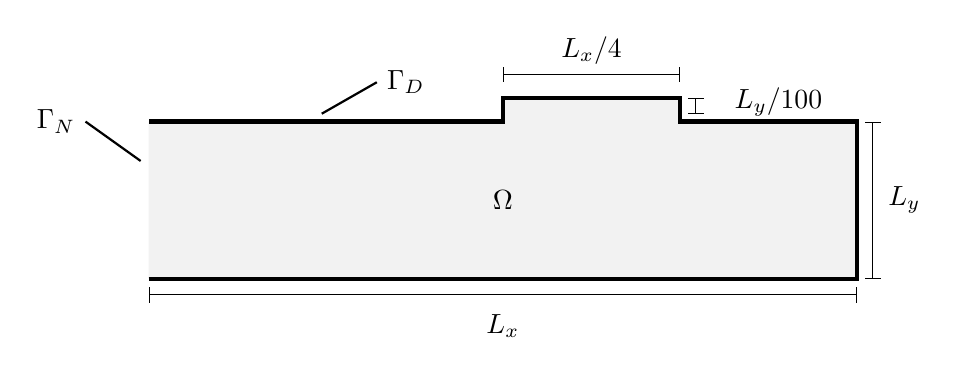
\begin{tikzpicture}
    \fill[black!5!white] (0, 0) to (9, 0) to (9, 2) to (6.75, 2) to (6.75, 2.3) to (4.5, 2.3) to (4.5, 2) to (0, 2);
    \draw[ultra thick] (0, 0) to (9, 0) to (9, 2) to (6.75, 2) to (6.75, 2.3) to (4.5, 2.3) to (4.5, 2) to (0, 2);
    \draw[thick] (-0.8, 2) node[left] {$\Gamma_N$} to (-0.1, 1.5);
    \draw[thick] (2.9, 2.5) node[right] {$\Gamma_D$} to (2.2, 2.1);
    \draw[|-|] (0, -0.2) to (9, -0.2);
    \draw[|-|] (9.2, 0) to (9.2, 2);
    \draw[|-|] (6.75, 2.6) to (4.5, 2.6);
    \draw[|-|] (6.95, 2.1) to (6.95, 2.3);
    \node at (4.5, -0.6) {$L_x$};
    \node at (9.6, 1) {$L_y$};
    \node at (5.626, 2.9) {$L_x / 4$};
    \node at (8, 2.25) {$L_y / 100$};
    \node at (4.5, 1) {$\Omega$};
\end{tikzpicture}

    \caption{A tiny cubby is introduced alongside one of the edges in order to
    break the linear dependence of solutions restricted to a trace. It extends
    along a quarter of the length of the cavity but extends outwards only by
    1/100-th of the height of the cavity.}
    \label{fig:rectangular-cavity-cubby}
\end{figure}

Desipte the only tiny perturbation in the geometry of the cavity, the improved
convergence behavior may immediately be seen in Figure \ref{fig:rectangular-cubby-trace-errornorm}.

\begin{figure}[ht]
    \centering
    %% Creator: Matplotlib, PGF backend
%%
%% To include the figure in your LaTeX document, write
%%   \input{<filename>.pgf}
%%
%% Make sure the required packages are loaded in your preamble
%%   \usepackage{pgf}
%%
%% Also ensure that all the required font packages are loaded; for instance,
%% the lmodern package is sometimes necessary when using math font.
%%   \usepackage{lmodern}
%%
%% Figures using additional raster images can only be included by \input if
%% they are in the same directory as the main LaTeX file. For loading figures
%% from other directories you can use the `import` package
%%   \usepackage{import}
%%
%% and then include the figures with
%%   \import{<path to file>}{<filename>.pgf}
%%
%% Matplotlib used the following preamble
%%   \usepackage{fontspec}
%%   \setmainfont{DejaVuSans.ttf}[Path=\detokenize{C:/Users/Fabio/Anaconda3/Lib/site-packages/matplotlib/mpl-data/fonts/ttf/}]
%%   \setsansfont{DejaVuSans.ttf}[Path=\detokenize{C:/Users/Fabio/Anaconda3/Lib/site-packages/matplotlib/mpl-data/fonts/ttf/}]
%%   \setmonofont{DejaVuSansMono.ttf}[Path=\detokenize{C:/Users/Fabio/Anaconda3/Lib/site-packages/matplotlib/mpl-data/fonts/ttf/}]
%%
\begingroup%
\makeatletter%
\begin{pgfpicture}%
\pgfpathrectangle{\pgfpointorigin}{\pgfqpoint{5.314460in}{3.950463in}}%
\pgfusepath{use as bounding box, clip}%
\begin{pgfscope}%
\pgfsetbuttcap%
\pgfsetmiterjoin%
\pgfsetlinewidth{0.000000pt}%
\definecolor{currentstroke}{rgb}{1.000000,1.000000,1.000000}%
\pgfsetstrokecolor{currentstroke}%
\pgfsetstrokeopacity{0.000000}%
\pgfsetdash{}{0pt}%
\pgfpathmoveto{\pgfqpoint{0.000000in}{0.000000in}}%
\pgfpathlineto{\pgfqpoint{5.314460in}{0.000000in}}%
\pgfpathlineto{\pgfqpoint{5.314460in}{3.950463in}}%
\pgfpathlineto{\pgfqpoint{0.000000in}{3.950463in}}%
\pgfpathlineto{\pgfqpoint{0.000000in}{0.000000in}}%
\pgfpathclose%
\pgfusepath{}%
\end{pgfscope}%
\begin{pgfscope}%
\pgfsetbuttcap%
\pgfsetmiterjoin%
\definecolor{currentfill}{rgb}{1.000000,1.000000,1.000000}%
\pgfsetfillcolor{currentfill}%
\pgfsetlinewidth{0.000000pt}%
\definecolor{currentstroke}{rgb}{0.000000,0.000000,0.000000}%
\pgfsetstrokecolor{currentstroke}%
\pgfsetstrokeopacity{0.000000}%
\pgfsetdash{}{0pt}%
\pgfpathmoveto{\pgfqpoint{0.816045in}{0.823031in}}%
\pgfpathlineto{\pgfqpoint{5.117295in}{0.823031in}}%
\pgfpathlineto{\pgfqpoint{5.117295in}{3.568486in}}%
\pgfpathlineto{\pgfqpoint{0.816045in}{3.568486in}}%
\pgfpathlineto{\pgfqpoint{0.816045in}{0.823031in}}%
\pgfpathclose%
\pgfusepath{fill}%
\end{pgfscope}%
\begin{pgfscope}%
\pgfsetbuttcap%
\pgfsetroundjoin%
\definecolor{currentfill}{rgb}{0.000000,0.000000,0.000000}%
\pgfsetfillcolor{currentfill}%
\pgfsetlinewidth{0.803000pt}%
\definecolor{currentstroke}{rgb}{0.000000,0.000000,0.000000}%
\pgfsetstrokecolor{currentstroke}%
\pgfsetdash{}{0pt}%
\pgfsys@defobject{currentmarker}{\pgfqpoint{0.000000in}{-0.048611in}}{\pgfqpoint{0.000000in}{0.000000in}}{%
\pgfpathmoveto{\pgfqpoint{0.000000in}{0.000000in}}%
\pgfpathlineto{\pgfqpoint{0.000000in}{-0.048611in}}%
\pgfusepath{stroke,fill}%
}%
\begin{pgfscope}%
\pgfsys@transformshift{0.816045in}{0.823031in}%
\pgfsys@useobject{currentmarker}{}%
\end{pgfscope}%
\end{pgfscope}%
\begin{pgfscope}%
\pgfsetbuttcap%
\pgfsetroundjoin%
\definecolor{currentfill}{rgb}{0.000000,0.000000,0.000000}%
\pgfsetfillcolor{currentfill}%
\pgfsetlinewidth{0.803000pt}%
\definecolor{currentstroke}{rgb}{0.000000,0.000000,0.000000}%
\pgfsetstrokecolor{currentstroke}%
\pgfsetdash{}{0pt}%
\pgfsys@defobject{currentmarker}{\pgfqpoint{0.000000in}{-0.048611in}}{\pgfqpoint{0.000000in}{0.000000in}}{%
\pgfpathmoveto{\pgfqpoint{0.000000in}{0.000000in}}%
\pgfpathlineto{\pgfqpoint{0.000000in}{-0.048611in}}%
\pgfusepath{stroke,fill}%
}%
\begin{pgfscope}%
\pgfsys@transformshift{1.676295in}{0.823031in}%
\pgfsys@useobject{currentmarker}{}%
\end{pgfscope}%
\end{pgfscope}%
\begin{pgfscope}%
\pgfsetbuttcap%
\pgfsetroundjoin%
\definecolor{currentfill}{rgb}{0.000000,0.000000,0.000000}%
\pgfsetfillcolor{currentfill}%
\pgfsetlinewidth{0.803000pt}%
\definecolor{currentstroke}{rgb}{0.000000,0.000000,0.000000}%
\pgfsetstrokecolor{currentstroke}%
\pgfsetdash{}{0pt}%
\pgfsys@defobject{currentmarker}{\pgfqpoint{0.000000in}{-0.048611in}}{\pgfqpoint{0.000000in}{0.000000in}}{%
\pgfpathmoveto{\pgfqpoint{0.000000in}{0.000000in}}%
\pgfpathlineto{\pgfqpoint{0.000000in}{-0.048611in}}%
\pgfusepath{stroke,fill}%
}%
\begin{pgfscope}%
\pgfsys@transformshift{2.536545in}{0.823031in}%
\pgfsys@useobject{currentmarker}{}%
\end{pgfscope}%
\end{pgfscope}%
\begin{pgfscope}%
\pgfsetbuttcap%
\pgfsetroundjoin%
\definecolor{currentfill}{rgb}{0.000000,0.000000,0.000000}%
\pgfsetfillcolor{currentfill}%
\pgfsetlinewidth{0.803000pt}%
\definecolor{currentstroke}{rgb}{0.000000,0.000000,0.000000}%
\pgfsetstrokecolor{currentstroke}%
\pgfsetdash{}{0pt}%
\pgfsys@defobject{currentmarker}{\pgfqpoint{0.000000in}{-0.048611in}}{\pgfqpoint{0.000000in}{0.000000in}}{%
\pgfpathmoveto{\pgfqpoint{0.000000in}{0.000000in}}%
\pgfpathlineto{\pgfqpoint{0.000000in}{-0.048611in}}%
\pgfusepath{stroke,fill}%
}%
\begin{pgfscope}%
\pgfsys@transformshift{3.396795in}{0.823031in}%
\pgfsys@useobject{currentmarker}{}%
\end{pgfscope}%
\end{pgfscope}%
\begin{pgfscope}%
\pgfsetbuttcap%
\pgfsetroundjoin%
\definecolor{currentfill}{rgb}{0.000000,0.000000,0.000000}%
\pgfsetfillcolor{currentfill}%
\pgfsetlinewidth{0.803000pt}%
\definecolor{currentstroke}{rgb}{0.000000,0.000000,0.000000}%
\pgfsetstrokecolor{currentstroke}%
\pgfsetdash{}{0pt}%
\pgfsys@defobject{currentmarker}{\pgfqpoint{0.000000in}{-0.048611in}}{\pgfqpoint{0.000000in}{0.000000in}}{%
\pgfpathmoveto{\pgfqpoint{0.000000in}{0.000000in}}%
\pgfpathlineto{\pgfqpoint{0.000000in}{-0.048611in}}%
\pgfusepath{stroke,fill}%
}%
\begin{pgfscope}%
\pgfsys@transformshift{4.257045in}{0.823031in}%
\pgfsys@useobject{currentmarker}{}%
\end{pgfscope}%
\end{pgfscope}%
\begin{pgfscope}%
\pgfsetbuttcap%
\pgfsetroundjoin%
\definecolor{currentfill}{rgb}{0.000000,0.000000,0.000000}%
\pgfsetfillcolor{currentfill}%
\pgfsetlinewidth{0.803000pt}%
\definecolor{currentstroke}{rgb}{0.000000,0.000000,0.000000}%
\pgfsetstrokecolor{currentstroke}%
\pgfsetdash{}{0pt}%
\pgfsys@defobject{currentmarker}{\pgfqpoint{0.000000in}{-0.048611in}}{\pgfqpoint{0.000000in}{0.000000in}}{%
\pgfpathmoveto{\pgfqpoint{0.000000in}{0.000000in}}%
\pgfpathlineto{\pgfqpoint{0.000000in}{-0.048611in}}%
\pgfusepath{stroke,fill}%
}%
\begin{pgfscope}%
\pgfsys@transformshift{5.117295in}{0.823031in}%
\pgfsys@useobject{currentmarker}{}%
\end{pgfscope}%
\end{pgfscope}%
\begin{pgfscope}%
\pgfpathrectangle{\pgfqpoint{0.816045in}{0.823031in}}{\pgfqpoint{4.301250in}{2.745455in}}%
\pgfusepath{clip}%
\pgfsetrectcap%
\pgfsetroundjoin%
\pgfsetlinewidth{0.803000pt}%
\definecolor{currentstroke}{rgb}{0.690196,0.690196,0.690196}%
\pgfsetstrokecolor{currentstroke}%
\pgfsetdash{}{0pt}%
\pgfpathmoveto{\pgfqpoint{0.816045in}{1.124514in}}%
\pgfpathlineto{\pgfqpoint{5.117295in}{1.124514in}}%
\pgfusepath{stroke}%
\end{pgfscope}%
\begin{pgfscope}%
\pgfsetbuttcap%
\pgfsetroundjoin%
\definecolor{currentfill}{rgb}{0.000000,0.000000,0.000000}%
\pgfsetfillcolor{currentfill}%
\pgfsetlinewidth{0.803000pt}%
\definecolor{currentstroke}{rgb}{0.000000,0.000000,0.000000}%
\pgfsetstrokecolor{currentstroke}%
\pgfsetdash{}{0pt}%
\pgfsys@defobject{currentmarker}{\pgfqpoint{-0.048611in}{0.000000in}}{\pgfqpoint{-0.000000in}{0.000000in}}{%
\pgfpathmoveto{\pgfqpoint{-0.000000in}{0.000000in}}%
\pgfpathlineto{\pgfqpoint{-0.048611in}{0.000000in}}%
\pgfusepath{stroke,fill}%
}%
\begin{pgfscope}%
\pgfsys@transformshift{0.816045in}{1.124514in}%
\pgfsys@useobject{currentmarker}{}%
\end{pgfscope}%
\end{pgfscope}%
\begin{pgfscope}%
\definecolor{textcolor}{rgb}{0.000000,0.000000,0.000000}%
\pgfsetstrokecolor{textcolor}%
\pgfsetfillcolor{textcolor}%
\pgftext[x=0.408944in, y=1.066477in, left, base]{\color{textcolor}\rmfamily\fontsize{11.000000}{13.200000}\selectfont \(\displaystyle {10^{-8}}\)}%
\end{pgfscope}%
\begin{pgfscope}%
\pgfpathrectangle{\pgfqpoint{0.816045in}{0.823031in}}{\pgfqpoint{4.301250in}{2.745455in}}%
\pgfusepath{clip}%
\pgfsetrectcap%
\pgfsetroundjoin%
\pgfsetlinewidth{0.803000pt}%
\definecolor{currentstroke}{rgb}{0.690196,0.690196,0.690196}%
\pgfsetstrokecolor{currentstroke}%
\pgfsetdash{}{0pt}%
\pgfpathmoveto{\pgfqpoint{0.816045in}{1.546434in}}%
\pgfpathlineto{\pgfqpoint{5.117295in}{1.546434in}}%
\pgfusepath{stroke}%
\end{pgfscope}%
\begin{pgfscope}%
\pgfsetbuttcap%
\pgfsetroundjoin%
\definecolor{currentfill}{rgb}{0.000000,0.000000,0.000000}%
\pgfsetfillcolor{currentfill}%
\pgfsetlinewidth{0.803000pt}%
\definecolor{currentstroke}{rgb}{0.000000,0.000000,0.000000}%
\pgfsetstrokecolor{currentstroke}%
\pgfsetdash{}{0pt}%
\pgfsys@defobject{currentmarker}{\pgfqpoint{-0.048611in}{0.000000in}}{\pgfqpoint{-0.000000in}{0.000000in}}{%
\pgfpathmoveto{\pgfqpoint{-0.000000in}{0.000000in}}%
\pgfpathlineto{\pgfqpoint{-0.048611in}{0.000000in}}%
\pgfusepath{stroke,fill}%
}%
\begin{pgfscope}%
\pgfsys@transformshift{0.816045in}{1.546434in}%
\pgfsys@useobject{currentmarker}{}%
\end{pgfscope}%
\end{pgfscope}%
\begin{pgfscope}%
\definecolor{textcolor}{rgb}{0.000000,0.000000,0.000000}%
\pgfsetstrokecolor{textcolor}%
\pgfsetfillcolor{textcolor}%
\pgftext[x=0.408944in, y=1.488396in, left, base]{\color{textcolor}\rmfamily\fontsize{11.000000}{13.200000}\selectfont \(\displaystyle {10^{-6}}\)}%
\end{pgfscope}%
\begin{pgfscope}%
\pgfpathrectangle{\pgfqpoint{0.816045in}{0.823031in}}{\pgfqpoint{4.301250in}{2.745455in}}%
\pgfusepath{clip}%
\pgfsetrectcap%
\pgfsetroundjoin%
\pgfsetlinewidth{0.803000pt}%
\definecolor{currentstroke}{rgb}{0.690196,0.690196,0.690196}%
\pgfsetstrokecolor{currentstroke}%
\pgfsetdash{}{0pt}%
\pgfpathmoveto{\pgfqpoint{0.816045in}{1.968353in}}%
\pgfpathlineto{\pgfqpoint{5.117295in}{1.968353in}}%
\pgfusepath{stroke}%
\end{pgfscope}%
\begin{pgfscope}%
\pgfsetbuttcap%
\pgfsetroundjoin%
\definecolor{currentfill}{rgb}{0.000000,0.000000,0.000000}%
\pgfsetfillcolor{currentfill}%
\pgfsetlinewidth{0.803000pt}%
\definecolor{currentstroke}{rgb}{0.000000,0.000000,0.000000}%
\pgfsetstrokecolor{currentstroke}%
\pgfsetdash{}{0pt}%
\pgfsys@defobject{currentmarker}{\pgfqpoint{-0.048611in}{0.000000in}}{\pgfqpoint{-0.000000in}{0.000000in}}{%
\pgfpathmoveto{\pgfqpoint{-0.000000in}{0.000000in}}%
\pgfpathlineto{\pgfqpoint{-0.048611in}{0.000000in}}%
\pgfusepath{stroke,fill}%
}%
\begin{pgfscope}%
\pgfsys@transformshift{0.816045in}{1.968353in}%
\pgfsys@useobject{currentmarker}{}%
\end{pgfscope}%
\end{pgfscope}%
\begin{pgfscope}%
\definecolor{textcolor}{rgb}{0.000000,0.000000,0.000000}%
\pgfsetstrokecolor{textcolor}%
\pgfsetfillcolor{textcolor}%
\pgftext[x=0.408944in, y=1.910316in, left, base]{\color{textcolor}\rmfamily\fontsize{11.000000}{13.200000}\selectfont \(\displaystyle {10^{-4}}\)}%
\end{pgfscope}%
\begin{pgfscope}%
\pgfpathrectangle{\pgfqpoint{0.816045in}{0.823031in}}{\pgfqpoint{4.301250in}{2.745455in}}%
\pgfusepath{clip}%
\pgfsetrectcap%
\pgfsetroundjoin%
\pgfsetlinewidth{0.803000pt}%
\definecolor{currentstroke}{rgb}{0.690196,0.690196,0.690196}%
\pgfsetstrokecolor{currentstroke}%
\pgfsetdash{}{0pt}%
\pgfpathmoveto{\pgfqpoint{0.816045in}{2.390273in}}%
\pgfpathlineto{\pgfqpoint{5.117295in}{2.390273in}}%
\pgfusepath{stroke}%
\end{pgfscope}%
\begin{pgfscope}%
\pgfsetbuttcap%
\pgfsetroundjoin%
\definecolor{currentfill}{rgb}{0.000000,0.000000,0.000000}%
\pgfsetfillcolor{currentfill}%
\pgfsetlinewidth{0.803000pt}%
\definecolor{currentstroke}{rgb}{0.000000,0.000000,0.000000}%
\pgfsetstrokecolor{currentstroke}%
\pgfsetdash{}{0pt}%
\pgfsys@defobject{currentmarker}{\pgfqpoint{-0.048611in}{0.000000in}}{\pgfqpoint{-0.000000in}{0.000000in}}{%
\pgfpathmoveto{\pgfqpoint{-0.000000in}{0.000000in}}%
\pgfpathlineto{\pgfqpoint{-0.048611in}{0.000000in}}%
\pgfusepath{stroke,fill}%
}%
\begin{pgfscope}%
\pgfsys@transformshift{0.816045in}{2.390273in}%
\pgfsys@useobject{currentmarker}{}%
\end{pgfscope}%
\end{pgfscope}%
\begin{pgfscope}%
\definecolor{textcolor}{rgb}{0.000000,0.000000,0.000000}%
\pgfsetstrokecolor{textcolor}%
\pgfsetfillcolor{textcolor}%
\pgftext[x=0.408944in, y=2.332235in, left, base]{\color{textcolor}\rmfamily\fontsize{11.000000}{13.200000}\selectfont \(\displaystyle {10^{-2}}\)}%
\end{pgfscope}%
\begin{pgfscope}%
\pgfpathrectangle{\pgfqpoint{0.816045in}{0.823031in}}{\pgfqpoint{4.301250in}{2.745455in}}%
\pgfusepath{clip}%
\pgfsetrectcap%
\pgfsetroundjoin%
\pgfsetlinewidth{0.803000pt}%
\definecolor{currentstroke}{rgb}{0.690196,0.690196,0.690196}%
\pgfsetstrokecolor{currentstroke}%
\pgfsetdash{}{0pt}%
\pgfpathmoveto{\pgfqpoint{0.816045in}{2.812192in}}%
\pgfpathlineto{\pgfqpoint{5.117295in}{2.812192in}}%
\pgfusepath{stroke}%
\end{pgfscope}%
\begin{pgfscope}%
\pgfsetbuttcap%
\pgfsetroundjoin%
\definecolor{currentfill}{rgb}{0.000000,0.000000,0.000000}%
\pgfsetfillcolor{currentfill}%
\pgfsetlinewidth{0.803000pt}%
\definecolor{currentstroke}{rgb}{0.000000,0.000000,0.000000}%
\pgfsetstrokecolor{currentstroke}%
\pgfsetdash{}{0pt}%
\pgfsys@defobject{currentmarker}{\pgfqpoint{-0.048611in}{0.000000in}}{\pgfqpoint{-0.000000in}{0.000000in}}{%
\pgfpathmoveto{\pgfqpoint{-0.000000in}{0.000000in}}%
\pgfpathlineto{\pgfqpoint{-0.048611in}{0.000000in}}%
\pgfusepath{stroke,fill}%
}%
\begin{pgfscope}%
\pgfsys@transformshift{0.816045in}{2.812192in}%
\pgfsys@useobject{currentmarker}{}%
\end{pgfscope}%
\end{pgfscope}%
\begin{pgfscope}%
\definecolor{textcolor}{rgb}{0.000000,0.000000,0.000000}%
\pgfsetstrokecolor{textcolor}%
\pgfsetfillcolor{textcolor}%
\pgftext[x=0.500767in, y=2.754155in, left, base]{\color{textcolor}\rmfamily\fontsize{11.000000}{13.200000}\selectfont \(\displaystyle {10^{0}}\)}%
\end{pgfscope}%
\begin{pgfscope}%
\pgfpathrectangle{\pgfqpoint{0.816045in}{0.823031in}}{\pgfqpoint{4.301250in}{2.745455in}}%
\pgfusepath{clip}%
\pgfsetrectcap%
\pgfsetroundjoin%
\pgfsetlinewidth{0.803000pt}%
\definecolor{currentstroke}{rgb}{0.690196,0.690196,0.690196}%
\pgfsetstrokecolor{currentstroke}%
\pgfsetdash{}{0pt}%
\pgfpathmoveto{\pgfqpoint{0.816045in}{3.234112in}}%
\pgfpathlineto{\pgfqpoint{5.117295in}{3.234112in}}%
\pgfusepath{stroke}%
\end{pgfscope}%
\begin{pgfscope}%
\pgfsetbuttcap%
\pgfsetroundjoin%
\definecolor{currentfill}{rgb}{0.000000,0.000000,0.000000}%
\pgfsetfillcolor{currentfill}%
\pgfsetlinewidth{0.803000pt}%
\definecolor{currentstroke}{rgb}{0.000000,0.000000,0.000000}%
\pgfsetstrokecolor{currentstroke}%
\pgfsetdash{}{0pt}%
\pgfsys@defobject{currentmarker}{\pgfqpoint{-0.048611in}{0.000000in}}{\pgfqpoint{-0.000000in}{0.000000in}}{%
\pgfpathmoveto{\pgfqpoint{-0.000000in}{0.000000in}}%
\pgfpathlineto{\pgfqpoint{-0.048611in}{0.000000in}}%
\pgfusepath{stroke,fill}%
}%
\begin{pgfscope}%
\pgfsys@transformshift{0.816045in}{3.234112in}%
\pgfsys@useobject{currentmarker}{}%
\end{pgfscope}%
\end{pgfscope}%
\begin{pgfscope}%
\definecolor{textcolor}{rgb}{0.000000,0.000000,0.000000}%
\pgfsetstrokecolor{textcolor}%
\pgfsetfillcolor{textcolor}%
\pgftext[x=0.500767in, y=3.176074in, left, base]{\color{textcolor}\rmfamily\fontsize{11.000000}{13.200000}\selectfont \(\displaystyle {10^{2}}\)}%
\end{pgfscope}%
\begin{pgfscope}%
\definecolor{textcolor}{rgb}{0.000000,0.000000,0.000000}%
\pgfsetstrokecolor{textcolor}%
\pgfsetfillcolor{textcolor}%
\pgftext[x=0.353389in,y=2.195759in,,bottom,rotate=90.000000]{\color{textcolor}\rmfamily\fontsize{11.000000}{13.200000}\selectfont \(\displaystyle ||\mathbf{\tilde{u}}_z^{(S)}|_{\Gamma_N}(\omega) - \mathbf{u}|_{\Gamma_N}(\omega)||_{M(\Gamma_N)} / ||\mathbf{\tilde{u}}_z^{(S)}|_{\Gamma_N}(\omega)||_{M(\Gamma_N)}\)}%
\end{pgfscope}%
\begin{pgfscope}%
\pgfpathrectangle{\pgfqpoint{0.816045in}{0.823031in}}{\pgfqpoint{4.301250in}{2.745455in}}%
\pgfusepath{clip}%
\pgfsetrectcap%
\pgfsetroundjoin%
\pgfsetlinewidth{1.505625pt}%
\definecolor{currentstroke}{rgb}{0.001462,0.000466,0.013866}%
\pgfsetstrokecolor{currentstroke}%
\pgfsetdash{}{0pt}%
\pgfpathmoveto{\pgfqpoint{0.813895in}{2.418879in}}%
\pgfpathlineto{\pgfqpoint{0.818200in}{2.421382in}}%
\pgfpathlineto{\pgfqpoint{0.822506in}{2.524354in}}%
\pgfpathlineto{\pgfqpoint{0.831117in}{2.606920in}}%
\pgfpathlineto{\pgfqpoint{0.839728in}{2.653565in}}%
\pgfpathlineto{\pgfqpoint{0.852645in}{2.701917in}}%
\pgfpathlineto{\pgfqpoint{0.869867in}{2.749927in}}%
\pgfpathlineto{\pgfqpoint{0.891395in}{2.799565in}}%
\pgfpathlineto{\pgfqpoint{0.934450in}{2.896812in}}%
\pgfpathlineto{\pgfqpoint{0.947367in}{2.932906in}}%
\pgfpathlineto{\pgfqpoint{0.960283in}{2.979168in}}%
\pgfpathlineto{\pgfqpoint{0.968894in}{3.022411in}}%
\pgfpathlineto{\pgfqpoint{0.973200in}{3.052088in}}%
\pgfpathlineto{\pgfqpoint{0.977506in}{3.093215in}}%
\pgfpathlineto{\pgfqpoint{0.981811in}{3.163152in}}%
\pgfpathlineto{\pgfqpoint{0.986117in}{3.299494in}}%
\pgfpathlineto{\pgfqpoint{0.990422in}{3.148337in}}%
\pgfpathlineto{\pgfqpoint{0.994728in}{3.092540in}}%
\pgfpathlineto{\pgfqpoint{1.003339in}{3.035979in}}%
\pgfpathlineto{\pgfqpoint{1.011950in}{3.003797in}}%
\pgfpathlineto{\pgfqpoint{1.020561in}{2.981793in}}%
\pgfpathlineto{\pgfqpoint{1.033478in}{2.958551in}}%
\pgfpathlineto{\pgfqpoint{1.046394in}{2.941917in}}%
\pgfpathlineto{\pgfqpoint{1.063617in}{2.925627in}}%
\pgfpathlineto{\pgfqpoint{1.080839in}{2.913472in}}%
\pgfpathlineto{\pgfqpoint{1.102367in}{2.901913in}}%
\pgfpathlineto{\pgfqpoint{1.128200in}{2.891459in}}%
\pgfpathlineto{\pgfqpoint{1.162644in}{2.881150in}}%
\pgfpathlineto{\pgfqpoint{1.205700in}{2.871837in}}%
\pgfpathlineto{\pgfqpoint{1.261672in}{2.863244in}}%
\pgfpathlineto{\pgfqpoint{1.334866in}{2.855447in}}%
\pgfpathlineto{\pgfqpoint{1.433894in}{2.848307in}}%
\pgfpathlineto{\pgfqpoint{1.571672in}{2.841751in}}%
\pgfpathlineto{\pgfqpoint{1.774033in}{2.835477in}}%
\pgfpathlineto{\pgfqpoint{2.140004in}{2.827747in}}%
\pgfpathlineto{\pgfqpoint{2.592087in}{2.817538in}}%
\pgfpathlineto{\pgfqpoint{2.794448in}{2.809933in}}%
\pgfpathlineto{\pgfqpoint{2.932226in}{2.801780in}}%
\pgfpathlineto{\pgfqpoint{3.031254in}{2.792955in}}%
\pgfpathlineto{\pgfqpoint{3.104448in}{2.783550in}}%
\pgfpathlineto{\pgfqpoint{3.160420in}{2.773560in}}%
\pgfpathlineto{\pgfqpoint{3.207781in}{2.762001in}}%
\pgfpathlineto{\pgfqpoint{3.242226in}{2.750757in}}%
\pgfpathlineto{\pgfqpoint{3.272364in}{2.737845in}}%
\pgfpathlineto{\pgfqpoint{3.298198in}{2.723222in}}%
\pgfpathlineto{\pgfqpoint{3.319725in}{2.707066in}}%
\pgfpathlineto{\pgfqpoint{3.336948in}{2.689985in}}%
\pgfpathlineto{\pgfqpoint{3.349864in}{2.673321in}}%
\pgfpathlineto{\pgfqpoint{3.362781in}{2.651271in}}%
\pgfpathlineto{\pgfqpoint{3.371392in}{2.631679in}}%
\pgfpathlineto{\pgfqpoint{3.380003in}{2.605275in}}%
\pgfpathlineto{\pgfqpoint{3.388614in}{2.565653in}}%
\pgfpathlineto{\pgfqpoint{3.392920in}{2.535427in}}%
\pgfpathlineto{\pgfqpoint{3.397225in}{2.488467in}}%
\pgfpathlineto{\pgfqpoint{3.401531in}{2.381986in}}%
\pgfpathlineto{\pgfqpoint{3.405837in}{2.402844in}}%
\pgfpathlineto{\pgfqpoint{3.410142in}{2.498632in}}%
\pgfpathlineto{\pgfqpoint{3.418753in}{2.576942in}}%
\pgfpathlineto{\pgfqpoint{3.427364in}{2.620412in}}%
\pgfpathlineto{\pgfqpoint{3.440281in}{2.663952in}}%
\pgfpathlineto{\pgfqpoint{3.453198in}{2.695626in}}%
\pgfpathlineto{\pgfqpoint{3.470420in}{2.728642in}}%
\pgfpathlineto{\pgfqpoint{3.491948in}{2.761896in}}%
\pgfpathlineto{\pgfqpoint{3.517781in}{2.795468in}}%
\pgfpathlineto{\pgfqpoint{3.552225in}{2.834857in}}%
\pgfpathlineto{\pgfqpoint{3.646947in}{2.940360in}}%
\pgfpathlineto{\pgfqpoint{3.672781in}{2.975413in}}%
\pgfpathlineto{\pgfqpoint{3.690003in}{3.003141in}}%
\pgfpathlineto{\pgfqpoint{3.707225in}{3.037173in}}%
\pgfpathlineto{\pgfqpoint{3.720142in}{3.070157in}}%
\pgfpathlineto{\pgfqpoint{3.728753in}{3.098712in}}%
\pgfpathlineto{\pgfqpoint{3.737364in}{3.137429in}}%
\pgfpathlineto{\pgfqpoint{3.741670in}{3.163989in}}%
\pgfpathlineto{\pgfqpoint{3.745975in}{3.200232in}}%
\pgfpathlineto{\pgfqpoint{3.750281in}{3.258665in}}%
\pgfpathlineto{\pgfqpoint{3.754586in}{3.443692in}}%
\pgfpathlineto{\pgfqpoint{3.758892in}{3.289989in}}%
\pgfpathlineto{\pgfqpoint{3.763197in}{3.219687in}}%
\pgfpathlineto{\pgfqpoint{3.771808in}{3.154914in}}%
\pgfpathlineto{\pgfqpoint{3.780419in}{3.119011in}}%
\pgfpathlineto{\pgfqpoint{3.789031in}{3.094477in}}%
\pgfpathlineto{\pgfqpoint{3.801947in}{3.068380in}}%
\pgfpathlineto{\pgfqpoint{3.814864in}{3.049496in}}%
\pgfpathlineto{\pgfqpoint{3.832086in}{3.030784in}}%
\pgfpathlineto{\pgfqpoint{3.849308in}{3.016678in}}%
\pgfpathlineto{\pgfqpoint{3.870836in}{3.003176in}}%
\pgfpathlineto{\pgfqpoint{3.896669in}{2.990967in}}%
\pgfpathlineto{\pgfqpoint{3.926808in}{2.980372in}}%
\pgfpathlineto{\pgfqpoint{3.961253in}{2.971512in}}%
\pgfpathlineto{\pgfqpoint{4.004308in}{2.963776in}}%
\pgfpathlineto{\pgfqpoint{4.055975in}{2.957925in}}%
\pgfpathlineto{\pgfqpoint{4.111947in}{2.954695in}}%
\pgfpathlineto{\pgfqpoint{4.176530in}{2.954211in}}%
\pgfpathlineto{\pgfqpoint{4.241113in}{2.956950in}}%
\pgfpathlineto{\pgfqpoint{4.301391in}{2.962684in}}%
\pgfpathlineto{\pgfqpoint{4.353058in}{2.970661in}}%
\pgfpathlineto{\pgfqpoint{4.396113in}{2.980261in}}%
\pgfpathlineto{\pgfqpoint{4.430558in}{2.990681in}}%
\pgfpathlineto{\pgfqpoint{4.460697in}{3.002682in}}%
\pgfpathlineto{\pgfqpoint{4.486530in}{3.016104in}}%
\pgfpathlineto{\pgfqpoint{4.508058in}{3.030579in}}%
\pgfpathlineto{\pgfqpoint{4.525280in}{3.045383in}}%
\pgfpathlineto{\pgfqpoint{4.542502in}{3.064603in}}%
\pgfpathlineto{\pgfqpoint{4.555419in}{3.083583in}}%
\pgfpathlineto{\pgfqpoint{4.568335in}{3.109182in}}%
\pgfpathlineto{\pgfqpoint{4.576946in}{3.132583in}}%
\pgfpathlineto{\pgfqpoint{4.585558in}{3.165563in}}%
\pgfpathlineto{\pgfqpoint{4.589863in}{3.188656in}}%
\pgfpathlineto{\pgfqpoint{4.594169in}{3.220259in}}%
\pgfpathlineto{\pgfqpoint{4.598474in}{3.269755in}}%
\pgfpathlineto{\pgfqpoint{4.602780in}{3.377288in}}%
\pgfpathlineto{\pgfqpoint{4.607085in}{3.325373in}}%
\pgfpathlineto{\pgfqpoint{4.611391in}{3.246223in}}%
\pgfpathlineto{\pgfqpoint{4.620002in}{3.173214in}}%
\pgfpathlineto{\pgfqpoint{4.628613in}{3.131667in}}%
\pgfpathlineto{\pgfqpoint{4.641530in}{3.090000in}}%
\pgfpathlineto{\pgfqpoint{4.654446in}{3.059911in}}%
\pgfpathlineto{\pgfqpoint{4.671669in}{3.028970in}}%
\pgfpathlineto{\pgfqpoint{4.688891in}{3.004072in}}%
\pgfpathlineto{\pgfqpoint{4.710419in}{2.978042in}}%
\pgfpathlineto{\pgfqpoint{4.736252in}{2.951445in}}%
\pgfpathlineto{\pgfqpoint{4.770696in}{2.920718in}}%
\pgfpathlineto{\pgfqpoint{4.818057in}{2.883282in}}%
\pgfpathlineto{\pgfqpoint{4.964446in}{2.771219in}}%
\pgfpathlineto{\pgfqpoint{4.994585in}{2.743249in}}%
\pgfpathlineto{\pgfqpoint{5.020418in}{2.715321in}}%
\pgfpathlineto{\pgfqpoint{5.041946in}{2.687355in}}%
\pgfpathlineto{\pgfqpoint{5.059168in}{2.659795in}}%
\pgfpathlineto{\pgfqpoint{5.072085in}{2.634023in}}%
\pgfpathlineto{\pgfqpoint{5.085001in}{2.600523in}}%
\pgfpathlineto{\pgfqpoint{5.093613in}{2.570365in}}%
\pgfpathlineto{\pgfqpoint{5.102224in}{2.527245in}}%
\pgfpathlineto{\pgfqpoint{5.106529in}{2.495577in}}%
\pgfpathlineto{\pgfqpoint{5.110835in}{2.447949in}}%
\pgfpathlineto{\pgfqpoint{5.115140in}{2.346524in}}%
\pgfpathlineto{\pgfqpoint{5.119446in}{2.345516in}}%
\pgfpathlineto{\pgfqpoint{5.119446in}{2.345516in}}%
\pgfusepath{stroke}%
\end{pgfscope}%
\begin{pgfscope}%
\pgfpathrectangle{\pgfqpoint{0.816045in}{0.823031in}}{\pgfqpoint{4.301250in}{2.745455in}}%
\pgfusepath{clip}%
\pgfsetrectcap%
\pgfsetroundjoin%
\pgfsetlinewidth{1.505625pt}%
\definecolor{currentstroke}{rgb}{0.155850,0.044559,0.325338}%
\pgfsetstrokecolor{currentstroke}%
\pgfsetdash{}{0pt}%
\pgfpathmoveto{\pgfqpoint{0.813895in}{2.420633in}}%
\pgfpathlineto{\pgfqpoint{0.818200in}{2.423139in}}%
\pgfpathlineto{\pgfqpoint{0.822506in}{2.526114in}}%
\pgfpathlineto{\pgfqpoint{0.831117in}{2.608685in}}%
\pgfpathlineto{\pgfqpoint{0.839728in}{2.655336in}}%
\pgfpathlineto{\pgfqpoint{0.852645in}{2.703696in}}%
\pgfpathlineto{\pgfqpoint{0.869867in}{2.751716in}}%
\pgfpathlineto{\pgfqpoint{0.891395in}{2.801366in}}%
\pgfpathlineto{\pgfqpoint{0.934450in}{2.898636in}}%
\pgfpathlineto{\pgfqpoint{0.947367in}{2.934737in}}%
\pgfpathlineto{\pgfqpoint{0.960283in}{2.981005in}}%
\pgfpathlineto{\pgfqpoint{0.968894in}{3.024253in}}%
\pgfpathlineto{\pgfqpoint{0.973200in}{3.053932in}}%
\pgfpathlineto{\pgfqpoint{0.977506in}{3.095061in}}%
\pgfpathlineto{\pgfqpoint{0.981811in}{3.165000in}}%
\pgfpathlineto{\pgfqpoint{0.986117in}{3.301344in}}%
\pgfpathlineto{\pgfqpoint{0.990422in}{3.150189in}}%
\pgfpathlineto{\pgfqpoint{0.994728in}{3.094395in}}%
\pgfpathlineto{\pgfqpoint{1.003339in}{3.037837in}}%
\pgfpathlineto{\pgfqpoint{1.011950in}{3.005659in}}%
\pgfpathlineto{\pgfqpoint{1.020561in}{2.983658in}}%
\pgfpathlineto{\pgfqpoint{1.033478in}{2.960422in}}%
\pgfpathlineto{\pgfqpoint{1.046394in}{2.943794in}}%
\pgfpathlineto{\pgfqpoint{1.063617in}{2.927510in}}%
\pgfpathlineto{\pgfqpoint{1.080839in}{2.915362in}}%
\pgfpathlineto{\pgfqpoint{1.102367in}{2.903810in}}%
\pgfpathlineto{\pgfqpoint{1.128200in}{2.893364in}}%
\pgfpathlineto{\pgfqpoint{1.162644in}{2.883065in}}%
\pgfpathlineto{\pgfqpoint{1.205700in}{2.873761in}}%
\pgfpathlineto{\pgfqpoint{1.261672in}{2.865177in}}%
\pgfpathlineto{\pgfqpoint{1.334866in}{2.857385in}}%
\pgfpathlineto{\pgfqpoint{1.433894in}{2.850238in}}%
\pgfpathlineto{\pgfqpoint{1.571672in}{2.843641in}}%
\pgfpathlineto{\pgfqpoint{1.778338in}{2.837121in}}%
\pgfpathlineto{\pgfqpoint{2.191671in}{2.827879in}}%
\pgfpathlineto{\pgfqpoint{2.587782in}{2.817831in}}%
\pgfpathlineto{\pgfqpoint{2.811670in}{2.809211in}}%
\pgfpathlineto{\pgfqpoint{2.979587in}{2.799797in}}%
\pgfpathlineto{\pgfqpoint{3.113059in}{2.789269in}}%
\pgfpathlineto{\pgfqpoint{3.220698in}{2.777699in}}%
\pgfpathlineto{\pgfqpoint{3.306809in}{2.765485in}}%
\pgfpathlineto{\pgfqpoint{3.380003in}{2.752105in}}%
\pgfpathlineto{\pgfqpoint{3.440281in}{2.738147in}}%
\pgfpathlineto{\pgfqpoint{3.491948in}{2.723203in}}%
\pgfpathlineto{\pgfqpoint{3.535003in}{2.707800in}}%
\pgfpathlineto{\pgfqpoint{3.573753in}{2.690693in}}%
\pgfpathlineto{\pgfqpoint{3.603892in}{2.674374in}}%
\pgfpathlineto{\pgfqpoint{3.629725in}{2.657389in}}%
\pgfpathlineto{\pgfqpoint{3.651253in}{2.640226in}}%
\pgfpathlineto{\pgfqpoint{3.672781in}{2.619036in}}%
\pgfpathlineto{\pgfqpoint{3.690003in}{2.597681in}}%
\pgfpathlineto{\pgfqpoint{3.702920in}{2.577668in}}%
\pgfpathlineto{\pgfqpoint{3.715836in}{2.552164in}}%
\pgfpathlineto{\pgfqpoint{3.724447in}{2.530234in}}%
\pgfpathlineto{\pgfqpoint{3.733058in}{2.501518in}}%
\pgfpathlineto{\pgfqpoint{3.741670in}{2.459781in}}%
\pgfpathlineto{\pgfqpoint{3.745975in}{2.428781in}}%
\pgfpathlineto{\pgfqpoint{3.750281in}{2.381801in}}%
\pgfpathlineto{\pgfqpoint{3.754586in}{2.280980in}}%
\pgfpathlineto{\pgfqpoint{3.758892in}{2.280715in}}%
\pgfpathlineto{\pgfqpoint{3.763197in}{2.381185in}}%
\pgfpathlineto{\pgfqpoint{3.771808in}{2.458385in}}%
\pgfpathlineto{\pgfqpoint{3.780419in}{2.499330in}}%
\pgfpathlineto{\pgfqpoint{3.789031in}{2.527245in}}%
\pgfpathlineto{\pgfqpoint{3.801947in}{2.557255in}}%
\pgfpathlineto{\pgfqpoint{3.814864in}{2.579381in}}%
\pgfpathlineto{\pgfqpoint{3.832086in}{2.601821in}}%
\pgfpathlineto{\pgfqpoint{3.849308in}{2.619180in}}%
\pgfpathlineto{\pgfqpoint{3.870836in}{2.636210in}}%
\pgfpathlineto{\pgfqpoint{3.896669in}{2.651954in}}%
\pgfpathlineto{\pgfqpoint{3.922503in}{2.664032in}}%
\pgfpathlineto{\pgfqpoint{3.952642in}{2.674619in}}%
\pgfpathlineto{\pgfqpoint{3.982780in}{2.682139in}}%
\pgfpathlineto{\pgfqpoint{4.017225in}{2.687472in}}%
\pgfpathlineto{\pgfqpoint{4.051669in}{2.689518in}}%
\pgfpathlineto{\pgfqpoint{4.086114in}{2.688152in}}%
\pgfpathlineto{\pgfqpoint{4.116252in}{2.683767in}}%
\pgfpathlineto{\pgfqpoint{4.142086in}{2.677085in}}%
\pgfpathlineto{\pgfqpoint{4.163614in}{2.668849in}}%
\pgfpathlineto{\pgfqpoint{4.185141in}{2.657314in}}%
\pgfpathlineto{\pgfqpoint{4.202363in}{2.644736in}}%
\pgfpathlineto{\pgfqpoint{4.219586in}{2.627686in}}%
\pgfpathlineto{\pgfqpoint{4.232502in}{2.610362in}}%
\pgfpathlineto{\pgfqpoint{4.245419in}{2.586559in}}%
\pgfpathlineto{\pgfqpoint{4.254030in}{2.564570in}}%
\pgfpathlineto{\pgfqpoint{4.262641in}{2.533468in}}%
\pgfpathlineto{\pgfqpoint{4.271252in}{2.482210in}}%
\pgfpathlineto{\pgfqpoint{4.275558in}{2.436714in}}%
\pgfpathlineto{\pgfqpoint{4.279863in}{2.337397in}}%
\pgfpathlineto{\pgfqpoint{4.284169in}{2.338587in}}%
\pgfpathlineto{\pgfqpoint{4.288475in}{2.440583in}}%
\pgfpathlineto{\pgfqpoint{4.297086in}{2.520846in}}%
\pgfpathlineto{\pgfqpoint{4.305697in}{2.564902in}}%
\pgfpathlineto{\pgfqpoint{4.318613in}{2.608802in}}%
\pgfpathlineto{\pgfqpoint{4.331530in}{2.640588in}}%
\pgfpathlineto{\pgfqpoint{4.348752in}{2.673543in}}%
\pgfpathlineto{\pgfqpoint{4.370280in}{2.706495in}}%
\pgfpathlineto{\pgfqpoint{4.396113in}{2.739483in}}%
\pgfpathlineto{\pgfqpoint{4.430558in}{2.777941in}}%
\pgfpathlineto{\pgfqpoint{4.503752in}{2.857682in}}%
\pgfpathlineto{\pgfqpoint{4.525280in}{2.885615in}}%
\pgfpathlineto{\pgfqpoint{4.542502in}{2.912130in}}%
\pgfpathlineto{\pgfqpoint{4.555419in}{2.936248in}}%
\pgfpathlineto{\pgfqpoint{4.568335in}{2.966724in}}%
\pgfpathlineto{\pgfqpoint{4.576946in}{2.993243in}}%
\pgfpathlineto{\pgfqpoint{4.585558in}{3.029239in}}%
\pgfpathlineto{\pgfqpoint{4.594169in}{3.086856in}}%
\pgfpathlineto{\pgfqpoint{4.598474in}{3.137777in}}%
\pgfpathlineto{\pgfqpoint{4.602780in}{3.246713in}}%
\pgfpathlineto{\pgfqpoint{4.607085in}{3.196179in}}%
\pgfpathlineto{\pgfqpoint{4.611391in}{3.118390in}}%
\pgfpathlineto{\pgfqpoint{4.620002in}{3.048039in}}%
\pgfpathlineto{\pgfqpoint{4.628613in}{3.009071in}}%
\pgfpathlineto{\pgfqpoint{4.637224in}{2.982070in}}%
\pgfpathlineto{\pgfqpoint{4.650141in}{2.952609in}}%
\pgfpathlineto{\pgfqpoint{4.663057in}{2.930459in}}%
\pgfpathlineto{\pgfqpoint{4.680280in}{2.907340in}}%
\pgfpathlineto{\pgfqpoint{4.701807in}{2.884489in}}%
\pgfpathlineto{\pgfqpoint{4.727641in}{2.862207in}}%
\pgfpathlineto{\pgfqpoint{4.762085in}{2.837377in}}%
\pgfpathlineto{\pgfqpoint{4.809446in}{2.807758in}}%
\pgfpathlineto{\pgfqpoint{4.938613in}{2.729248in}}%
\pgfpathlineto{\pgfqpoint{4.973057in}{2.704074in}}%
\pgfpathlineto{\pgfqpoint{5.003196in}{2.678167in}}%
\pgfpathlineto{\pgfqpoint{5.024724in}{2.656049in}}%
\pgfpathlineto{\pgfqpoint{5.041946in}{2.634927in}}%
\pgfpathlineto{\pgfqpoint{5.059168in}{2.608973in}}%
\pgfpathlineto{\pgfqpoint{5.072085in}{2.584367in}}%
\pgfpathlineto{\pgfqpoint{5.085001in}{2.552000in}}%
\pgfpathlineto{\pgfqpoint{5.093613in}{2.522580in}}%
\pgfpathlineto{\pgfqpoint{5.102224in}{2.480185in}}%
\pgfpathlineto{\pgfqpoint{5.106529in}{2.448874in}}%
\pgfpathlineto{\pgfqpoint{5.110835in}{2.401600in}}%
\pgfpathlineto{\pgfqpoint{5.115140in}{2.300526in}}%
\pgfpathlineto{\pgfqpoint{5.119446in}{2.299865in}}%
\pgfpathlineto{\pgfqpoint{5.119446in}{2.299865in}}%
\pgfusepath{stroke}%
\end{pgfscope}%
\begin{pgfscope}%
\pgfpathrectangle{\pgfqpoint{0.816045in}{0.823031in}}{\pgfqpoint{4.301250in}{2.745455in}}%
\pgfusepath{clip}%
\pgfsetrectcap%
\pgfsetroundjoin%
\pgfsetlinewidth{1.505625pt}%
\definecolor{currentstroke}{rgb}{0.397674,0.083257,0.433183}%
\pgfsetstrokecolor{currentstroke}%
\pgfsetdash{}{0pt}%
\pgfpathmoveto{\pgfqpoint{0.813895in}{2.262946in}}%
\pgfpathlineto{\pgfqpoint{0.818200in}{2.264931in}}%
\pgfpathlineto{\pgfqpoint{0.822506in}{2.367384in}}%
\pgfpathlineto{\pgfqpoint{0.831117in}{2.448910in}}%
\pgfpathlineto{\pgfqpoint{0.839728in}{2.494512in}}%
\pgfpathlineto{\pgfqpoint{0.852645in}{2.541293in}}%
\pgfpathlineto{\pgfqpoint{0.869867in}{2.587198in}}%
\pgfpathlineto{\pgfqpoint{0.891395in}{2.634186in}}%
\pgfpathlineto{\pgfqpoint{0.930145in}{2.715825in}}%
\pgfpathlineto{\pgfqpoint{0.947367in}{2.760534in}}%
\pgfpathlineto{\pgfqpoint{0.960283in}{2.805161in}}%
\pgfpathlineto{\pgfqpoint{0.968894in}{2.847310in}}%
\pgfpathlineto{\pgfqpoint{0.973200in}{2.876437in}}%
\pgfpathlineto{\pgfqpoint{0.977506in}{2.917014in}}%
\pgfpathlineto{\pgfqpoint{0.981811in}{2.986400in}}%
\pgfpathlineto{\pgfqpoint{0.986117in}{3.122190in}}%
\pgfpathlineto{\pgfqpoint{0.990422in}{2.970481in}}%
\pgfpathlineto{\pgfqpoint{0.994728in}{2.914130in}}%
\pgfpathlineto{\pgfqpoint{1.003339in}{2.856458in}}%
\pgfpathlineto{\pgfqpoint{1.011950in}{2.823161in}}%
\pgfpathlineto{\pgfqpoint{1.020561in}{2.800038in}}%
\pgfpathlineto{\pgfqpoint{1.033478in}{2.775111in}}%
\pgfpathlineto{\pgfqpoint{1.046394in}{2.756781in}}%
\pgfpathlineto{\pgfqpoint{1.063617in}{2.738213in}}%
\pgfpathlineto{\pgfqpoint{1.085144in}{2.720605in}}%
\pgfpathlineto{\pgfqpoint{1.110978in}{2.704322in}}%
\pgfpathlineto{\pgfqpoint{1.141117in}{2.689313in}}%
\pgfpathlineto{\pgfqpoint{1.179867in}{2.673771in}}%
\pgfpathlineto{\pgfqpoint{1.231533in}{2.656852in}}%
\pgfpathlineto{\pgfqpoint{1.300422in}{2.637960in}}%
\pgfpathlineto{\pgfqpoint{1.399450in}{2.614300in}}%
\pgfpathlineto{\pgfqpoint{1.804171in}{2.520720in}}%
\pgfpathlineto{\pgfqpoint{1.903199in}{2.493149in}}%
\pgfpathlineto{\pgfqpoint{1.980699in}{2.468543in}}%
\pgfpathlineto{\pgfqpoint{2.045282in}{2.445023in}}%
\pgfpathlineto{\pgfqpoint{2.101254in}{2.421403in}}%
\pgfpathlineto{\pgfqpoint{2.148616in}{2.397973in}}%
\pgfpathlineto{\pgfqpoint{2.187366in}{2.375332in}}%
\pgfpathlineto{\pgfqpoint{2.217504in}{2.354541in}}%
\pgfpathlineto{\pgfqpoint{2.243338in}{2.333460in}}%
\pgfpathlineto{\pgfqpoint{2.264865in}{2.312511in}}%
\pgfpathlineto{\pgfqpoint{2.286393in}{2.286856in}}%
\pgfpathlineto{\pgfqpoint{2.303615in}{2.260921in}}%
\pgfpathlineto{\pgfqpoint{2.316532in}{2.236242in}}%
\pgfpathlineto{\pgfqpoint{2.329449in}{2.203728in}}%
\pgfpathlineto{\pgfqpoint{2.338060in}{2.174167in}}%
\pgfpathlineto{\pgfqpoint{2.346671in}{2.131594in}}%
\pgfpathlineto{\pgfqpoint{2.350976in}{2.100178in}}%
\pgfpathlineto{\pgfqpoint{2.355282in}{2.052781in}}%
\pgfpathlineto{\pgfqpoint{2.359588in}{1.951514in}}%
\pgfpathlineto{\pgfqpoint{2.363893in}{1.950963in}}%
\pgfpathlineto{\pgfqpoint{2.368199in}{2.050993in}}%
\pgfpathlineto{\pgfqpoint{2.376810in}{2.127386in}}%
\pgfpathlineto{\pgfqpoint{2.385421in}{2.167542in}}%
\pgfpathlineto{\pgfqpoint{2.394032in}{2.194681in}}%
\pgfpathlineto{\pgfqpoint{2.406949in}{2.223542in}}%
\pgfpathlineto{\pgfqpoint{2.419865in}{2.244536in}}%
\pgfpathlineto{\pgfqpoint{2.437087in}{2.265486in}}%
\pgfpathlineto{\pgfqpoint{2.454310in}{2.281365in}}%
\pgfpathlineto{\pgfqpoint{2.475837in}{2.296527in}}%
\pgfpathlineto{\pgfqpoint{2.497365in}{2.307994in}}%
\pgfpathlineto{\pgfqpoint{2.523198in}{2.318061in}}%
\pgfpathlineto{\pgfqpoint{2.549032in}{2.324717in}}%
\pgfpathlineto{\pgfqpoint{2.574865in}{2.328008in}}%
\pgfpathlineto{\pgfqpoint{2.596393in}{2.327706in}}%
\pgfpathlineto{\pgfqpoint{2.613615in}{2.324721in}}%
\pgfpathlineto{\pgfqpoint{2.626532in}{2.320126in}}%
\pgfpathlineto{\pgfqpoint{2.639448in}{2.312397in}}%
\pgfpathlineto{\pgfqpoint{2.648059in}{2.304534in}}%
\pgfpathlineto{\pgfqpoint{2.656671in}{2.293163in}}%
\pgfpathlineto{\pgfqpoint{2.665282in}{2.275835in}}%
\pgfpathlineto{\pgfqpoint{2.673893in}{2.246524in}}%
\pgfpathlineto{\pgfqpoint{2.678198in}{2.222211in}}%
\pgfpathlineto{\pgfqpoint{2.682504in}{2.182292in}}%
\pgfpathlineto{\pgfqpoint{2.686809in}{2.088941in}}%
\pgfpathlineto{\pgfqpoint{2.691115in}{2.096770in}}%
\pgfpathlineto{\pgfqpoint{2.695421in}{2.205802in}}%
\pgfpathlineto{\pgfqpoint{2.704032in}{2.302425in}}%
\pgfpathlineto{\pgfqpoint{2.716948in}{2.396255in}}%
\pgfpathlineto{\pgfqpoint{2.729865in}{2.490858in}}%
\pgfpathlineto{\pgfqpoint{2.734171in}{2.532647in}}%
\pgfpathlineto{\pgfqpoint{2.738476in}{2.591308in}}%
\pgfpathlineto{\pgfqpoint{2.742782in}{2.716820in}}%
\pgfpathlineto{\pgfqpoint{2.747087in}{2.681281in}}%
\pgfpathlineto{\pgfqpoint{2.751393in}{2.599893in}}%
\pgfpathlineto{\pgfqpoint{2.755698in}{2.562325in}}%
\pgfpathlineto{\pgfqpoint{2.764309in}{2.522301in}}%
\pgfpathlineto{\pgfqpoint{2.772920in}{2.500078in}}%
\pgfpathlineto{\pgfqpoint{2.781532in}{2.485619in}}%
\pgfpathlineto{\pgfqpoint{2.794448in}{2.471321in}}%
\pgfpathlineto{\pgfqpoint{2.807365in}{2.461864in}}%
\pgfpathlineto{\pgfqpoint{2.824587in}{2.453339in}}%
\pgfpathlineto{\pgfqpoint{2.846115in}{2.446309in}}%
\pgfpathlineto{\pgfqpoint{2.876254in}{2.439978in}}%
\pgfpathlineto{\pgfqpoint{2.923615in}{2.433808in}}%
\pgfpathlineto{\pgfqpoint{3.014031in}{2.426029in}}%
\pgfpathlineto{\pgfqpoint{3.160420in}{2.412966in}}%
\pgfpathlineto{\pgfqpoint{3.255142in}{2.401246in}}%
\pgfpathlineto{\pgfqpoint{3.332642in}{2.388657in}}%
\pgfpathlineto{\pgfqpoint{3.401531in}{2.374369in}}%
\pgfpathlineto{\pgfqpoint{3.457503in}{2.359842in}}%
\pgfpathlineto{\pgfqpoint{3.509170in}{2.343219in}}%
\pgfpathlineto{\pgfqpoint{3.552225in}{2.326054in}}%
\pgfpathlineto{\pgfqpoint{3.586670in}{2.309231in}}%
\pgfpathlineto{\pgfqpoint{3.616809in}{2.291269in}}%
\pgfpathlineto{\pgfqpoint{3.642642in}{2.272369in}}%
\pgfpathlineto{\pgfqpoint{3.664170in}{2.252950in}}%
\pgfpathlineto{\pgfqpoint{3.681392in}{2.233816in}}%
\pgfpathlineto{\pgfqpoint{3.698614in}{2.209706in}}%
\pgfpathlineto{\pgfqpoint{3.711531in}{2.186388in}}%
\pgfpathlineto{\pgfqpoint{3.724447in}{2.155230in}}%
\pgfpathlineto{\pgfqpoint{3.733058in}{2.126573in}}%
\pgfpathlineto{\pgfqpoint{3.741670in}{2.084904in}}%
\pgfpathlineto{\pgfqpoint{3.745975in}{2.053942in}}%
\pgfpathlineto{\pgfqpoint{3.750281in}{2.007004in}}%
\pgfpathlineto{\pgfqpoint{3.754586in}{1.906226in}}%
\pgfpathlineto{\pgfqpoint{3.758892in}{1.906008in}}%
\pgfpathlineto{\pgfqpoint{3.763197in}{2.006528in}}%
\pgfpathlineto{\pgfqpoint{3.771808in}{2.083835in}}%
\pgfpathlineto{\pgfqpoint{3.780419in}{2.124899in}}%
\pgfpathlineto{\pgfqpoint{3.789031in}{2.152946in}}%
\pgfpathlineto{\pgfqpoint{3.801947in}{2.183177in}}%
\pgfpathlineto{\pgfqpoint{3.814864in}{2.205554in}}%
\pgfpathlineto{\pgfqpoint{3.832086in}{2.228379in}}%
\pgfpathlineto{\pgfqpoint{3.849308in}{2.246180in}}%
\pgfpathlineto{\pgfqpoint{3.870836in}{2.263851in}}%
\pgfpathlineto{\pgfqpoint{3.896669in}{2.280498in}}%
\pgfpathlineto{\pgfqpoint{3.922503in}{2.293637in}}%
\pgfpathlineto{\pgfqpoint{3.952642in}{2.305671in}}%
\pgfpathlineto{\pgfqpoint{3.987086in}{2.315988in}}%
\pgfpathlineto{\pgfqpoint{4.021530in}{2.323182in}}%
\pgfpathlineto{\pgfqpoint{4.055975in}{2.327434in}}%
\pgfpathlineto{\pgfqpoint{4.090419in}{2.328589in}}%
\pgfpathlineto{\pgfqpoint{4.120558in}{2.326624in}}%
\pgfpathlineto{\pgfqpoint{4.146391in}{2.322125in}}%
\pgfpathlineto{\pgfqpoint{4.167919in}{2.315722in}}%
\pgfpathlineto{\pgfqpoint{4.189447in}{2.305930in}}%
\pgfpathlineto{\pgfqpoint{4.206669in}{2.294545in}}%
\pgfpathlineto{\pgfqpoint{4.219586in}{2.282927in}}%
\pgfpathlineto{\pgfqpoint{4.232502in}{2.267318in}}%
\pgfpathlineto{\pgfqpoint{4.245419in}{2.245280in}}%
\pgfpathlineto{\pgfqpoint{4.254030in}{2.224493in}}%
\pgfpathlineto{\pgfqpoint{4.262641in}{2.194616in}}%
\pgfpathlineto{\pgfqpoint{4.266947in}{2.173507in}}%
\pgfpathlineto{\pgfqpoint{4.271252in}{2.144604in}}%
\pgfpathlineto{\pgfqpoint{4.275558in}{2.099738in}}%
\pgfpathlineto{\pgfqpoint{4.279863in}{2.001057in}}%
\pgfpathlineto{\pgfqpoint{4.284169in}{2.002888in}}%
\pgfpathlineto{\pgfqpoint{4.288475in}{2.105531in}}%
\pgfpathlineto{\pgfqpoint{4.297086in}{2.187101in}}%
\pgfpathlineto{\pgfqpoint{4.305697in}{2.232486in}}%
\pgfpathlineto{\pgfqpoint{4.318613in}{2.278416in}}%
\pgfpathlineto{\pgfqpoint{4.331530in}{2.312275in}}%
\pgfpathlineto{\pgfqpoint{4.348752in}{2.348063in}}%
\pgfpathlineto{\pgfqpoint{4.370280in}{2.384662in}}%
\pgfpathlineto{\pgfqpoint{4.396113in}{2.422175in}}%
\pgfpathlineto{\pgfqpoint{4.434863in}{2.472292in}}%
\pgfpathlineto{\pgfqpoint{4.499447in}{2.554805in}}%
\pgfpathlineto{\pgfqpoint{4.525280in}{2.593101in}}%
\pgfpathlineto{\pgfqpoint{4.542502in}{2.623165in}}%
\pgfpathlineto{\pgfqpoint{4.559724in}{2.660144in}}%
\pgfpathlineto{\pgfqpoint{4.572641in}{2.696502in}}%
\pgfpathlineto{\pgfqpoint{4.581252in}{2.728819in}}%
\pgfpathlineto{\pgfqpoint{4.589863in}{2.774846in}}%
\pgfpathlineto{\pgfqpoint{4.594169in}{2.808825in}}%
\pgfpathlineto{\pgfqpoint{4.598474in}{2.860676in}}%
\pgfpathlineto{\pgfqpoint{4.602780in}{2.970544in}}%
\pgfpathlineto{\pgfqpoint{4.607085in}{2.920946in}}%
\pgfpathlineto{\pgfqpoint{4.611391in}{2.844095in}}%
\pgfpathlineto{\pgfqpoint{4.620002in}{2.775629in}}%
\pgfpathlineto{\pgfqpoint{4.628613in}{2.738556in}}%
\pgfpathlineto{\pgfqpoint{4.637224in}{2.713460in}}%
\pgfpathlineto{\pgfqpoint{4.650141in}{2.686875in}}%
\pgfpathlineto{\pgfqpoint{4.663057in}{2.667623in}}%
\pgfpathlineto{\pgfqpoint{4.680280in}{2.648403in}}%
\pgfpathlineto{\pgfqpoint{4.697502in}{2.633671in}}%
\pgfpathlineto{\pgfqpoint{4.719030in}{2.619148in}}%
\pgfpathlineto{\pgfqpoint{4.744863in}{2.605288in}}%
\pgfpathlineto{\pgfqpoint{4.779307in}{2.590373in}}%
\pgfpathlineto{\pgfqpoint{4.830974in}{2.571738in}}%
\pgfpathlineto{\pgfqpoint{4.925696in}{2.538216in}}%
\pgfpathlineto{\pgfqpoint{4.964446in}{2.521022in}}%
\pgfpathlineto{\pgfqpoint{4.994585in}{2.504243in}}%
\pgfpathlineto{\pgfqpoint{5.016113in}{2.489244in}}%
\pgfpathlineto{\pgfqpoint{5.037640in}{2.470217in}}%
\pgfpathlineto{\pgfqpoint{5.054863in}{2.450356in}}%
\pgfpathlineto{\pgfqpoint{5.067779in}{2.431045in}}%
\pgfpathlineto{\pgfqpoint{5.080696in}{2.405345in}}%
\pgfpathlineto{\pgfqpoint{5.089307in}{2.382133in}}%
\pgfpathlineto{\pgfqpoint{5.097918in}{2.349840in}}%
\pgfpathlineto{\pgfqpoint{5.106529in}{2.297419in}}%
\pgfpathlineto{\pgfqpoint{5.110835in}{2.251352in}}%
\pgfpathlineto{\pgfqpoint{5.115140in}{2.151488in}}%
\pgfpathlineto{\pgfqpoint{5.119446in}{2.152041in}}%
\pgfpathlineto{\pgfqpoint{5.119446in}{2.152041in}}%
\pgfusepath{stroke}%
\end{pgfscope}%
\begin{pgfscope}%
\pgfpathrectangle{\pgfqpoint{0.816045in}{0.823031in}}{\pgfqpoint{4.301250in}{2.745455in}}%
\pgfusepath{clip}%
\pgfsetrectcap%
\pgfsetroundjoin%
\pgfsetlinewidth{1.505625pt}%
\definecolor{currentstroke}{rgb}{0.621685,0.164184,0.388781}%
\pgfsetstrokecolor{currentstroke}%
\pgfsetdash{}{0pt}%
\pgfpathmoveto{\pgfqpoint{0.813895in}{1.887700in}}%
\pgfpathlineto{\pgfqpoint{0.818200in}{1.888232in}}%
\pgfpathlineto{\pgfqpoint{0.822506in}{1.989222in}}%
\pgfpathlineto{\pgfqpoint{0.831117in}{2.067784in}}%
\pgfpathlineto{\pgfqpoint{0.839728in}{2.110372in}}%
\pgfpathlineto{\pgfqpoint{0.852645in}{2.152535in}}%
\pgfpathlineto{\pgfqpoint{0.865561in}{2.183244in}}%
\pgfpathlineto{\pgfqpoint{0.882783in}{2.216089in}}%
\pgfpathlineto{\pgfqpoint{0.943061in}{2.322967in}}%
\pgfpathlineto{\pgfqpoint{0.955978in}{2.357278in}}%
\pgfpathlineto{\pgfqpoint{0.964589in}{2.388876in}}%
\pgfpathlineto{\pgfqpoint{0.973200in}{2.436719in}}%
\pgfpathlineto{\pgfqpoint{0.977506in}{2.475113in}}%
\pgfpathlineto{\pgfqpoint{0.981811in}{2.542281in}}%
\pgfpathlineto{\pgfqpoint{0.986117in}{2.675817in}}%
\pgfpathlineto{\pgfqpoint{0.990422in}{2.521816in}}%
\pgfpathlineto{\pgfqpoint{0.994728in}{2.463135in}}%
\pgfpathlineto{\pgfqpoint{1.003339in}{2.400678in}}%
\pgfpathlineto{\pgfqpoint{1.011950in}{2.362419in}}%
\pgfpathlineto{\pgfqpoint{1.024867in}{2.322173in}}%
\pgfpathlineto{\pgfqpoint{1.037783in}{2.291566in}}%
\pgfpathlineto{\pgfqpoint{1.055006in}{2.257947in}}%
\pgfpathlineto{\pgfqpoint{1.085144in}{2.207262in}}%
\pgfpathlineto{\pgfqpoint{1.123894in}{2.142292in}}%
\pgfpathlineto{\pgfqpoint{1.141117in}{2.108643in}}%
\pgfpathlineto{\pgfqpoint{1.154033in}{2.078781in}}%
\pgfpathlineto{\pgfqpoint{1.166950in}{2.041509in}}%
\pgfpathlineto{\pgfqpoint{1.175561in}{2.008980in}}%
\pgfpathlineto{\pgfqpoint{1.184172in}{1.963584in}}%
\pgfpathlineto{\pgfqpoint{1.188478in}{1.930806in}}%
\pgfpathlineto{\pgfqpoint{1.192783in}{1.882075in}}%
\pgfpathlineto{\pgfqpoint{1.197089in}{1.779478in}}%
\pgfpathlineto{\pgfqpoint{1.201394in}{1.777760in}}%
\pgfpathlineto{\pgfqpoint{1.205700in}{1.876517in}}%
\pgfpathlineto{\pgfqpoint{1.214311in}{1.950505in}}%
\pgfpathlineto{\pgfqpoint{1.222922in}{1.988364in}}%
\pgfpathlineto{\pgfqpoint{1.231533in}{2.013304in}}%
\pgfpathlineto{\pgfqpoint{1.244450in}{2.039038in}}%
\pgfpathlineto{\pgfqpoint{1.257366in}{2.057099in}}%
\pgfpathlineto{\pgfqpoint{1.270283in}{2.070630in}}%
\pgfpathlineto{\pgfqpoint{1.287505in}{2.084192in}}%
\pgfpathlineto{\pgfqpoint{1.309033in}{2.096479in}}%
\pgfpathlineto{\pgfqpoint{1.334866in}{2.106816in}}%
\pgfpathlineto{\pgfqpoint{1.365005in}{2.114909in}}%
\pgfpathlineto{\pgfqpoint{1.399450in}{2.120657in}}%
\pgfpathlineto{\pgfqpoint{1.438200in}{2.124038in}}%
\pgfpathlineto{\pgfqpoint{1.485561in}{2.125016in}}%
\pgfpathlineto{\pgfqpoint{1.541533in}{2.122889in}}%
\pgfpathlineto{\pgfqpoint{1.601811in}{2.117546in}}%
\pgfpathlineto{\pgfqpoint{1.670699in}{2.108264in}}%
\pgfpathlineto{\pgfqpoint{1.743894in}{2.095113in}}%
\pgfpathlineto{\pgfqpoint{1.817088in}{2.078685in}}%
\pgfpathlineto{\pgfqpoint{1.885977in}{2.060076in}}%
\pgfpathlineto{\pgfqpoint{1.950560in}{2.039501in}}%
\pgfpathlineto{\pgfqpoint{2.010838in}{2.017038in}}%
\pgfpathlineto{\pgfqpoint{2.062505in}{1.994668in}}%
\pgfpathlineto{\pgfqpoint{2.109866in}{1.970908in}}%
\pgfpathlineto{\pgfqpoint{2.152921in}{1.945722in}}%
\pgfpathlineto{\pgfqpoint{2.187366in}{1.922223in}}%
\pgfpathlineto{\pgfqpoint{2.217504in}{1.898267in}}%
\pgfpathlineto{\pgfqpoint{2.243338in}{1.874179in}}%
\pgfpathlineto{\pgfqpoint{2.264865in}{1.850500in}}%
\pgfpathlineto{\pgfqpoint{2.286393in}{1.821897in}}%
\pgfpathlineto{\pgfqpoint{2.303615in}{1.793437in}}%
\pgfpathlineto{\pgfqpoint{2.316532in}{1.766759in}}%
\pgfpathlineto{\pgfqpoint{2.329449in}{1.732152in}}%
\pgfpathlineto{\pgfqpoint{2.338060in}{1.701141in}}%
\pgfpathlineto{\pgfqpoint{2.346671in}{1.657073in}}%
\pgfpathlineto{\pgfqpoint{2.350976in}{1.624891in}}%
\pgfpathlineto{\pgfqpoint{2.355282in}{1.576717in}}%
\pgfpathlineto{\pgfqpoint{2.359588in}{1.474660in}}%
\pgfpathlineto{\pgfqpoint{2.363893in}{1.473307in}}%
\pgfpathlineto{\pgfqpoint{2.368199in}{1.572522in}}%
\pgfpathlineto{\pgfqpoint{2.376810in}{1.647245in}}%
\pgfpathlineto{\pgfqpoint{2.385421in}{1.685678in}}%
\pgfpathlineto{\pgfqpoint{2.394032in}{1.711035in}}%
\pgfpathlineto{\pgfqpoint{2.406949in}{1.737113in}}%
\pgfpathlineto{\pgfqpoint{2.419865in}{1.755181in}}%
\pgfpathlineto{\pgfqpoint{2.432782in}{1.768381in}}%
\pgfpathlineto{\pgfqpoint{2.450004in}{1.780963in}}%
\pgfpathlineto{\pgfqpoint{2.467226in}{1.789482in}}%
\pgfpathlineto{\pgfqpoint{2.484449in}{1.794944in}}%
\pgfpathlineto{\pgfqpoint{2.505976in}{1.798291in}}%
\pgfpathlineto{\pgfqpoint{2.527504in}{1.798254in}}%
\pgfpathlineto{\pgfqpoint{2.549032in}{1.794975in}}%
\pgfpathlineto{\pgfqpoint{2.570560in}{1.788244in}}%
\pgfpathlineto{\pgfqpoint{2.587782in}{1.779965in}}%
\pgfpathlineto{\pgfqpoint{2.605004in}{1.768440in}}%
\pgfpathlineto{\pgfqpoint{2.622226in}{1.752506in}}%
\pgfpathlineto{\pgfqpoint{2.635143in}{1.736354in}}%
\pgfpathlineto{\pgfqpoint{2.648059in}{1.714568in}}%
\pgfpathlineto{\pgfqpoint{2.656671in}{1.695053in}}%
\pgfpathlineto{\pgfqpoint{2.665282in}{1.668716in}}%
\pgfpathlineto{\pgfqpoint{2.673893in}{1.629331in}}%
\pgfpathlineto{\pgfqpoint{2.678198in}{1.599501in}}%
\pgfpathlineto{\pgfqpoint{2.682504in}{1.553691in}}%
\pgfpathlineto{\pgfqpoint{2.686809in}{1.454018in}}%
\pgfpathlineto{\pgfqpoint{2.691115in}{1.455032in}}%
\pgfpathlineto{\pgfqpoint{2.695421in}{1.556675in}}%
\pgfpathlineto{\pgfqpoint{2.704032in}{1.636348in}}%
\pgfpathlineto{\pgfqpoint{2.712643in}{1.679975in}}%
\pgfpathlineto{\pgfqpoint{2.725559in}{1.724220in}}%
\pgfpathlineto{\pgfqpoint{2.738476in}{1.765649in}}%
\pgfpathlineto{\pgfqpoint{2.742782in}{1.821951in}}%
\pgfpathlineto{\pgfqpoint{2.747087in}{1.727001in}}%
\pgfpathlineto{\pgfqpoint{2.751393in}{1.757480in}}%
\pgfpathlineto{\pgfqpoint{2.760004in}{1.778449in}}%
\pgfpathlineto{\pgfqpoint{2.772920in}{1.798388in}}%
\pgfpathlineto{\pgfqpoint{2.790143in}{1.818931in}}%
\pgfpathlineto{\pgfqpoint{2.811670in}{1.839698in}}%
\pgfpathlineto{\pgfqpoint{2.837504in}{1.860122in}}%
\pgfpathlineto{\pgfqpoint{2.867643in}{1.879766in}}%
\pgfpathlineto{\pgfqpoint{2.902087in}{1.898327in}}%
\pgfpathlineto{\pgfqpoint{2.940837in}{1.915584in}}%
\pgfpathlineto{\pgfqpoint{2.983892in}{1.931362in}}%
\pgfpathlineto{\pgfqpoint{3.031254in}{1.945491in}}%
\pgfpathlineto{\pgfqpoint{3.082920in}{1.957787in}}%
\pgfpathlineto{\pgfqpoint{3.138892in}{1.968016in}}%
\pgfpathlineto{\pgfqpoint{3.199170in}{1.975864in}}%
\pgfpathlineto{\pgfqpoint{3.259448in}{1.980655in}}%
\pgfpathlineto{\pgfqpoint{3.319725in}{1.982411in}}%
\pgfpathlineto{\pgfqpoint{3.375698in}{1.981163in}}%
\pgfpathlineto{\pgfqpoint{3.431670in}{1.976778in}}%
\pgfpathlineto{\pgfqpoint{3.479031in}{1.970131in}}%
\pgfpathlineto{\pgfqpoint{3.522086in}{1.961145in}}%
\pgfpathlineto{\pgfqpoint{3.560836in}{1.949918in}}%
\pgfpathlineto{\pgfqpoint{3.595281in}{1.936531in}}%
\pgfpathlineto{\pgfqpoint{3.621114in}{1.923563in}}%
\pgfpathlineto{\pgfqpoint{3.646947in}{1.907001in}}%
\pgfpathlineto{\pgfqpoint{3.668475in}{1.889174in}}%
\pgfpathlineto{\pgfqpoint{3.685697in}{1.870915in}}%
\pgfpathlineto{\pgfqpoint{3.698614in}{1.853687in}}%
\pgfpathlineto{\pgfqpoint{3.711531in}{1.831762in}}%
\pgfpathlineto{\pgfqpoint{3.724447in}{1.801979in}}%
\pgfpathlineto{\pgfqpoint{3.733058in}{1.774227in}}%
\pgfpathlineto{\pgfqpoint{3.741670in}{1.733455in}}%
\pgfpathlineto{\pgfqpoint{3.745975in}{1.702938in}}%
\pgfpathlineto{\pgfqpoint{3.750281in}{1.656443in}}%
\pgfpathlineto{\pgfqpoint{3.754586in}{1.556107in}}%
\pgfpathlineto{\pgfqpoint{3.758892in}{1.556328in}}%
\pgfpathlineto{\pgfqpoint{3.763197in}{1.657285in}}%
\pgfpathlineto{\pgfqpoint{3.771808in}{1.735461in}}%
\pgfpathlineto{\pgfqpoint{3.780419in}{1.777385in}}%
\pgfpathlineto{\pgfqpoint{3.789031in}{1.806285in}}%
\pgfpathlineto{\pgfqpoint{3.801947in}{1.837782in}}%
\pgfpathlineto{\pgfqpoint{3.814864in}{1.861406in}}%
\pgfpathlineto{\pgfqpoint{3.832086in}{1.885869in}}%
\pgfpathlineto{\pgfqpoint{3.849308in}{1.905280in}}%
\pgfpathlineto{\pgfqpoint{3.870836in}{1.924922in}}%
\pgfpathlineto{\pgfqpoint{3.896669in}{1.943880in}}%
\pgfpathlineto{\pgfqpoint{3.926808in}{1.961555in}}%
\pgfpathlineto{\pgfqpoint{3.956947in}{1.975691in}}%
\pgfpathlineto{\pgfqpoint{3.991391in}{1.988408in}}%
\pgfpathlineto{\pgfqpoint{4.025836in}{1.997949in}}%
\pgfpathlineto{\pgfqpoint{4.060280in}{2.004456in}}%
\pgfpathlineto{\pgfqpoint{4.094725in}{2.007730in}}%
\pgfpathlineto{\pgfqpoint{4.124864in}{2.007461in}}%
\pgfpathlineto{\pgfqpoint{4.150697in}{2.004239in}}%
\pgfpathlineto{\pgfqpoint{4.172225in}{1.998706in}}%
\pgfpathlineto{\pgfqpoint{4.189447in}{1.991702in}}%
\pgfpathlineto{\pgfqpoint{4.206669in}{1.981438in}}%
\pgfpathlineto{\pgfqpoint{4.219586in}{1.970648in}}%
\pgfpathlineto{\pgfqpoint{4.232502in}{1.955855in}}%
\pgfpathlineto{\pgfqpoint{4.245419in}{1.934622in}}%
\pgfpathlineto{\pgfqpoint{4.254030in}{1.914366in}}%
\pgfpathlineto{\pgfqpoint{4.262641in}{1.885014in}}%
\pgfpathlineto{\pgfqpoint{4.266947in}{1.864166in}}%
\pgfpathlineto{\pgfqpoint{4.271252in}{1.835522in}}%
\pgfpathlineto{\pgfqpoint{4.275558in}{1.790915in}}%
\pgfpathlineto{\pgfqpoint{4.279863in}{1.692491in}}%
\pgfpathlineto{\pgfqpoint{4.284169in}{1.694578in}}%
\pgfpathlineto{\pgfqpoint{4.288475in}{1.797476in}}%
\pgfpathlineto{\pgfqpoint{4.297086in}{1.879552in}}%
\pgfpathlineto{\pgfqpoint{4.305697in}{1.925437in}}%
\pgfpathlineto{\pgfqpoint{4.318613in}{1.972109in}}%
\pgfpathlineto{\pgfqpoint{4.331530in}{2.006700in}}%
\pgfpathlineto{\pgfqpoint{4.348752in}{2.043446in}}%
\pgfpathlineto{\pgfqpoint{4.370280in}{2.081215in}}%
\pgfpathlineto{\pgfqpoint{4.396113in}{2.120093in}}%
\pgfpathlineto{\pgfqpoint{4.434863in}{2.172175in}}%
\pgfpathlineto{\pgfqpoint{4.503752in}{2.263940in}}%
\pgfpathlineto{\pgfqpoint{4.529585in}{2.304439in}}%
\pgfpathlineto{\pgfqpoint{4.546808in}{2.336589in}}%
\pgfpathlineto{\pgfqpoint{4.559724in}{2.365683in}}%
\pgfpathlineto{\pgfqpoint{4.572641in}{2.402566in}}%
\pgfpathlineto{\pgfqpoint{4.581252in}{2.435226in}}%
\pgfpathlineto{\pgfqpoint{4.589863in}{2.481592in}}%
\pgfpathlineto{\pgfqpoint{4.594169in}{2.515738in}}%
\pgfpathlineto{\pgfqpoint{4.598474in}{2.567756in}}%
\pgfpathlineto{\pgfqpoint{4.602780in}{2.677788in}}%
\pgfpathlineto{\pgfqpoint{4.607085in}{2.628354in}}%
\pgfpathlineto{\pgfqpoint{4.611391in}{2.551665in}}%
\pgfpathlineto{\pgfqpoint{4.620002in}{2.483518in}}%
\pgfpathlineto{\pgfqpoint{4.628613in}{2.446760in}}%
\pgfpathlineto{\pgfqpoint{4.637224in}{2.421973in}}%
\pgfpathlineto{\pgfqpoint{4.650141in}{2.395843in}}%
\pgfpathlineto{\pgfqpoint{4.663057in}{2.377033in}}%
\pgfpathlineto{\pgfqpoint{4.680280in}{2.358383in}}%
\pgfpathlineto{\pgfqpoint{4.697502in}{2.344197in}}%
\pgfpathlineto{\pgfqpoint{4.719030in}{2.330326in}}%
\pgfpathlineto{\pgfqpoint{4.744863in}{2.317200in}}%
\pgfpathlineto{\pgfqpoint{4.779307in}{2.303178in}}%
\pgfpathlineto{\pgfqpoint{4.835280in}{2.284314in}}%
\pgfpathlineto{\pgfqpoint{4.921391in}{2.255275in}}%
\pgfpathlineto{\pgfqpoint{4.960141in}{2.238815in}}%
\pgfpathlineto{\pgfqpoint{4.990279in}{2.222716in}}%
\pgfpathlineto{\pgfqpoint{5.016113in}{2.205090in}}%
\pgfpathlineto{\pgfqpoint{5.037640in}{2.186015in}}%
\pgfpathlineto{\pgfqpoint{5.054863in}{2.166068in}}%
\pgfpathlineto{\pgfqpoint{5.067779in}{2.146663in}}%
\pgfpathlineto{\pgfqpoint{5.080696in}{2.120843in}}%
\pgfpathlineto{\pgfqpoint{5.089307in}{2.097537in}}%
\pgfpathlineto{\pgfqpoint{5.097918in}{2.065136in}}%
\pgfpathlineto{\pgfqpoint{5.106529in}{2.012595in}}%
\pgfpathlineto{\pgfqpoint{5.110835in}{1.966463in}}%
\pgfpathlineto{\pgfqpoint{5.115140in}{1.866532in}}%
\pgfpathlineto{\pgfqpoint{5.119446in}{1.867014in}}%
\pgfpathlineto{\pgfqpoint{5.119446in}{1.867014in}}%
\pgfusepath{stroke}%
\end{pgfscope}%
\begin{pgfscope}%
\pgfpathrectangle{\pgfqpoint{0.816045in}{0.823031in}}{\pgfqpoint{4.301250in}{2.745455in}}%
\pgfusepath{clip}%
\pgfsetrectcap%
\pgfsetroundjoin%
\pgfsetlinewidth{1.505625pt}%
\definecolor{currentstroke}{rgb}{0.832299,0.283913,0.257383}%
\pgfsetstrokecolor{currentstroke}%
\pgfsetdash{}{0pt}%
\pgfpathmoveto{\pgfqpoint{0.813895in}{1.571393in}}%
\pgfpathlineto{\pgfqpoint{0.818200in}{1.571221in}}%
\pgfpathlineto{\pgfqpoint{0.822506in}{1.671503in}}%
\pgfpathlineto{\pgfqpoint{0.831117in}{1.748644in}}%
\pgfpathlineto{\pgfqpoint{0.839728in}{1.789799in}}%
\pgfpathlineto{\pgfqpoint{0.848339in}{1.818216in}}%
\pgfpathlineto{\pgfqpoint{0.861256in}{1.849607in}}%
\pgfpathlineto{\pgfqpoint{0.878478in}{1.881254in}}%
\pgfpathlineto{\pgfqpoint{0.904311in}{1.920255in}}%
\pgfpathlineto{\pgfqpoint{0.930145in}{1.959930in}}%
\pgfpathlineto{\pgfqpoint{0.943061in}{1.984223in}}%
\pgfpathlineto{\pgfqpoint{0.955978in}{2.016119in}}%
\pgfpathlineto{\pgfqpoint{0.964589in}{2.046086in}}%
\pgfpathlineto{\pgfqpoint{0.973200in}{2.092280in}}%
\pgfpathlineto{\pgfqpoint{0.977506in}{2.129844in}}%
\pgfpathlineto{\pgfqpoint{0.981811in}{2.196177in}}%
\pgfpathlineto{\pgfqpoint{0.986117in}{2.328874in}}%
\pgfpathlineto{\pgfqpoint{0.990422in}{2.174029in}}%
\pgfpathlineto{\pgfqpoint{0.994728in}{2.114499in}}%
\pgfpathlineto{\pgfqpoint{1.003339in}{2.050331in}}%
\pgfpathlineto{\pgfqpoint{1.011950in}{2.010341in}}%
\pgfpathlineto{\pgfqpoint{1.024867in}{1.967462in}}%
\pgfpathlineto{\pgfqpoint{1.042089in}{1.924291in}}%
\pgfpathlineto{\pgfqpoint{1.063617in}{1.879922in}}%
\pgfpathlineto{\pgfqpoint{1.136811in}{1.737774in}}%
\pgfpathlineto{\pgfqpoint{1.154033in}{1.694689in}}%
\pgfpathlineto{\pgfqpoint{1.166950in}{1.654100in}}%
\pgfpathlineto{\pgfqpoint{1.175561in}{1.619314in}}%
\pgfpathlineto{\pgfqpoint{1.184172in}{1.571620in}}%
\pgfpathlineto{\pgfqpoint{1.188478in}{1.537678in}}%
\pgfpathlineto{\pgfqpoint{1.192783in}{1.487772in}}%
\pgfpathlineto{\pgfqpoint{1.197089in}{1.383989in}}%
\pgfpathlineto{\pgfqpoint{1.201394in}{1.381073in}}%
\pgfpathlineto{\pgfqpoint{1.205700in}{1.478622in}}%
\pgfpathlineto{\pgfqpoint{1.210005in}{1.522370in}}%
\pgfpathlineto{\pgfqpoint{1.218616in}{1.570154in}}%
\pgfpathlineto{\pgfqpoint{1.227228in}{1.597806in}}%
\pgfpathlineto{\pgfqpoint{1.235839in}{1.616364in}}%
\pgfpathlineto{\pgfqpoint{1.248755in}{1.635040in}}%
\pgfpathlineto{\pgfqpoint{1.261672in}{1.647247in}}%
\pgfpathlineto{\pgfqpoint{1.274589in}{1.655408in}}%
\pgfpathlineto{\pgfqpoint{1.291811in}{1.662071in}}%
\pgfpathlineto{\pgfqpoint{1.309033in}{1.665331in}}%
\pgfpathlineto{\pgfqpoint{1.330561in}{1.665923in}}%
\pgfpathlineto{\pgfqpoint{1.352089in}{1.663509in}}%
\pgfpathlineto{\pgfqpoint{1.377922in}{1.657333in}}%
\pgfpathlineto{\pgfqpoint{1.403755in}{1.647920in}}%
\pgfpathlineto{\pgfqpoint{1.429588in}{1.635262in}}%
\pgfpathlineto{\pgfqpoint{1.455422in}{1.618978in}}%
\pgfpathlineto{\pgfqpoint{1.476950in}{1.602005in}}%
\pgfpathlineto{\pgfqpoint{1.498477in}{1.580884in}}%
\pgfpathlineto{\pgfqpoint{1.515700in}{1.559741in}}%
\pgfpathlineto{\pgfqpoint{1.532922in}{1.532761in}}%
\pgfpathlineto{\pgfqpoint{1.545838in}{1.506283in}}%
\pgfpathlineto{\pgfqpoint{1.554449in}{1.483656in}}%
\pgfpathlineto{\pgfqpoint{1.563061in}{1.454209in}}%
\pgfpathlineto{\pgfqpoint{1.571672in}{1.411707in}}%
\pgfpathlineto{\pgfqpoint{1.575977in}{1.380311in}}%
\pgfpathlineto{\pgfqpoint{1.580283in}{1.332921in}}%
\pgfpathlineto{\pgfqpoint{1.584588in}{1.231635in}}%
\pgfpathlineto{\pgfqpoint{1.588894in}{1.231144in}}%
\pgfpathlineto{\pgfqpoint{1.593199in}{1.331136in}}%
\pgfpathlineto{\pgfqpoint{1.601811in}{1.407470in}}%
\pgfpathlineto{\pgfqpoint{1.610422in}{1.447540in}}%
\pgfpathlineto{\pgfqpoint{1.619033in}{1.474566in}}%
\pgfpathlineto{\pgfqpoint{1.631949in}{1.503215in}}%
\pgfpathlineto{\pgfqpoint{1.644866in}{1.523951in}}%
\pgfpathlineto{\pgfqpoint{1.662088in}{1.544506in}}%
\pgfpathlineto{\pgfqpoint{1.679310in}{1.559956in}}%
\pgfpathlineto{\pgfqpoint{1.700838in}{1.574591in}}%
\pgfpathlineto{\pgfqpoint{1.722366in}{1.585621in}}%
\pgfpathlineto{\pgfqpoint{1.748199in}{1.595454in}}%
\pgfpathlineto{\pgfqpoint{1.778338in}{1.603456in}}%
\pgfpathlineto{\pgfqpoint{1.812783in}{1.609138in}}%
\pgfpathlineto{\pgfqpoint{1.851533in}{1.612076in}}%
\pgfpathlineto{\pgfqpoint{1.890282in}{1.612011in}}%
\pgfpathlineto{\pgfqpoint{1.933338in}{1.608888in}}%
\pgfpathlineto{\pgfqpoint{1.976393in}{1.602812in}}%
\pgfpathlineto{\pgfqpoint{2.019449in}{1.593845in}}%
\pgfpathlineto{\pgfqpoint{2.062505in}{1.581866in}}%
\pgfpathlineto{\pgfqpoint{2.105560in}{1.566538in}}%
\pgfpathlineto{\pgfqpoint{2.144310in}{1.549358in}}%
\pgfpathlineto{\pgfqpoint{2.178754in}{1.530727in}}%
\pgfpathlineto{\pgfqpoint{2.208893in}{1.511050in}}%
\pgfpathlineto{\pgfqpoint{2.234727in}{1.490814in}}%
\pgfpathlineto{\pgfqpoint{2.256254in}{1.470675in}}%
\pgfpathlineto{\pgfqpoint{2.277782in}{1.446265in}}%
\pgfpathlineto{\pgfqpoint{2.295004in}{1.422153in}}%
\pgfpathlineto{\pgfqpoint{2.307921in}{1.399964in}}%
\pgfpathlineto{\pgfqpoint{2.320838in}{1.372186in}}%
\pgfpathlineto{\pgfqpoint{2.333754in}{1.334624in}}%
\pgfpathlineto{\pgfqpoint{2.342365in}{1.298978in}}%
\pgfpathlineto{\pgfqpoint{2.350976in}{1.243093in}}%
\pgfpathlineto{\pgfqpoint{2.355282in}{1.195243in}}%
\pgfpathlineto{\pgfqpoint{2.359588in}{1.093507in}}%
\pgfpathlineto{\pgfqpoint{2.363893in}{1.092474in}}%
\pgfpathlineto{\pgfqpoint{2.368199in}{1.192003in}}%
\pgfpathlineto{\pgfqpoint{2.376810in}{1.267349in}}%
\pgfpathlineto{\pgfqpoint{2.385421in}{1.306392in}}%
\pgfpathlineto{\pgfqpoint{2.394032in}{1.332349in}}%
\pgfpathlineto{\pgfqpoint{2.406949in}{1.359305in}}%
\pgfpathlineto{\pgfqpoint{2.419865in}{1.378226in}}%
\pgfpathlineto{\pgfqpoint{2.432782in}{1.392256in}}%
\pgfpathlineto{\pgfqpoint{2.450004in}{1.405909in}}%
\pgfpathlineto{\pgfqpoint{2.467226in}{1.415460in}}%
\pgfpathlineto{\pgfqpoint{2.484449in}{1.421915in}}%
\pgfpathlineto{\pgfqpoint{2.505976in}{1.426452in}}%
\pgfpathlineto{\pgfqpoint{2.527504in}{1.427549in}}%
\pgfpathlineto{\pgfqpoint{2.549032in}{1.425351in}}%
\pgfpathlineto{\pgfqpoint{2.570560in}{1.419651in}}%
\pgfpathlineto{\pgfqpoint{2.587782in}{1.412159in}}%
\pgfpathlineto{\pgfqpoint{2.605004in}{1.401392in}}%
\pgfpathlineto{\pgfqpoint{2.622226in}{1.386185in}}%
\pgfpathlineto{\pgfqpoint{2.635143in}{1.370559in}}%
\pgfpathlineto{\pgfqpoint{2.648059in}{1.349283in}}%
\pgfpathlineto{\pgfqpoint{2.656671in}{1.330100in}}%
\pgfpathlineto{\pgfqpoint{2.665282in}{1.304087in}}%
\pgfpathlineto{\pgfqpoint{2.673893in}{1.265020in}}%
\pgfpathlineto{\pgfqpoint{2.678198in}{1.235347in}}%
\pgfpathlineto{\pgfqpoint{2.682504in}{1.189692in}}%
\pgfpathlineto{\pgfqpoint{2.686809in}{1.090168in}}%
\pgfpathlineto{\pgfqpoint{2.691115in}{1.091337in}}%
\pgfpathlineto{\pgfqpoint{2.695421in}{1.193128in}}%
\pgfpathlineto{\pgfqpoint{2.704032in}{1.273095in}}%
\pgfpathlineto{\pgfqpoint{2.712643in}{1.317010in}}%
\pgfpathlineto{\pgfqpoint{2.725559in}{1.361674in}}%
\pgfpathlineto{\pgfqpoint{2.738476in}{1.403507in}}%
\pgfpathlineto{\pgfqpoint{2.742782in}{1.459941in}}%
\pgfpathlineto{\pgfqpoint{2.747087in}{1.365126in}}%
\pgfpathlineto{\pgfqpoint{2.751393in}{1.395732in}}%
\pgfpathlineto{\pgfqpoint{2.760004in}{1.416953in}}%
\pgfpathlineto{\pgfqpoint{2.772920in}{1.437260in}}%
\pgfpathlineto{\pgfqpoint{2.790143in}{1.458273in}}%
\pgfpathlineto{\pgfqpoint{2.811670in}{1.479594in}}%
\pgfpathlineto{\pgfqpoint{2.837504in}{1.500635in}}%
\pgfpathlineto{\pgfqpoint{2.867643in}{1.520936in}}%
\pgfpathlineto{\pgfqpoint{2.902087in}{1.540165in}}%
\pgfpathlineto{\pgfqpoint{2.940837in}{1.558072in}}%
\pgfpathlineto{\pgfqpoint{2.983892in}{1.574450in}}%
\pgfpathlineto{\pgfqpoint{3.031254in}{1.589094in}}%
\pgfpathlineto{\pgfqpoint{3.082920in}{1.601782in}}%
\pgfpathlineto{\pgfqpoint{3.138892in}{1.612240in}}%
\pgfpathlineto{\pgfqpoint{3.194864in}{1.619661in}}%
\pgfpathlineto{\pgfqpoint{3.255142in}{1.624478in}}%
\pgfpathlineto{\pgfqpoint{3.315420in}{1.626035in}}%
\pgfpathlineto{\pgfqpoint{3.371392in}{1.624415in}}%
\pgfpathlineto{\pgfqpoint{3.423059in}{1.620000in}}%
\pgfpathlineto{\pgfqpoint{3.470420in}{1.613066in}}%
\pgfpathlineto{\pgfqpoint{3.513475in}{1.603822in}}%
\pgfpathlineto{\pgfqpoint{3.552225in}{1.592436in}}%
\pgfpathlineto{\pgfqpoint{3.586670in}{1.579069in}}%
\pgfpathlineto{\pgfqpoint{3.616809in}{1.563915in}}%
\pgfpathlineto{\pgfqpoint{3.642642in}{1.547266in}}%
\pgfpathlineto{\pgfqpoint{3.664170in}{1.529616in}}%
\pgfpathlineto{\pgfqpoint{3.681392in}{1.511829in}}%
\pgfpathlineto{\pgfqpoint{3.698614in}{1.489004in}}%
\pgfpathlineto{\pgfqpoint{3.711531in}{1.466612in}}%
\pgfpathlineto{\pgfqpoint{3.724447in}{1.436347in}}%
\pgfpathlineto{\pgfqpoint{3.733058in}{1.408266in}}%
\pgfpathlineto{\pgfqpoint{3.741670in}{1.367159in}}%
\pgfpathlineto{\pgfqpoint{3.745975in}{1.336472in}}%
\pgfpathlineto{\pgfqpoint{3.750281in}{1.289805in}}%
\pgfpathlineto{\pgfqpoint{3.754586in}{1.189296in}}%
\pgfpathlineto{\pgfqpoint{3.758892in}{1.189342in}}%
\pgfpathlineto{\pgfqpoint{3.763197in}{1.290122in}}%
\pgfpathlineto{\pgfqpoint{3.771808in}{1.367940in}}%
\pgfpathlineto{\pgfqpoint{3.780419in}{1.409500in}}%
\pgfpathlineto{\pgfqpoint{3.789031in}{1.438029in}}%
\pgfpathlineto{\pgfqpoint{3.801947in}{1.468957in}}%
\pgfpathlineto{\pgfqpoint{3.814864in}{1.491997in}}%
\pgfpathlineto{\pgfqpoint{3.832086in}{1.515656in}}%
\pgfpathlineto{\pgfqpoint{3.849308in}{1.534234in}}%
\pgfpathlineto{\pgfqpoint{3.870836in}{1.552795in}}%
\pgfpathlineto{\pgfqpoint{3.896669in}{1.570392in}}%
\pgfpathlineto{\pgfqpoint{3.922503in}{1.584349in}}%
\pgfpathlineto{\pgfqpoint{3.952642in}{1.597172in}}%
\pgfpathlineto{\pgfqpoint{3.987086in}{1.608167in}}%
\pgfpathlineto{\pgfqpoint{4.021530in}{1.615796in}}%
\pgfpathlineto{\pgfqpoint{4.055975in}{1.620233in}}%
\pgfpathlineto{\pgfqpoint{4.090419in}{1.621314in}}%
\pgfpathlineto{\pgfqpoint{4.120558in}{1.619063in}}%
\pgfpathlineto{\pgfqpoint{4.146391in}{1.614148in}}%
\pgfpathlineto{\pgfqpoint{4.167919in}{1.607273in}}%
\pgfpathlineto{\pgfqpoint{4.189447in}{1.596891in}}%
\pgfpathlineto{\pgfqpoint{4.206669in}{1.584945in}}%
\pgfpathlineto{\pgfqpoint{4.219586in}{1.572855in}}%
\pgfpathlineto{\pgfqpoint{4.232502in}{1.556726in}}%
\pgfpathlineto{\pgfqpoint{4.245419in}{1.534119in}}%
\pgfpathlineto{\pgfqpoint{4.254030in}{1.512927in}}%
\pgfpathlineto{\pgfqpoint{4.262641in}{1.482621in}}%
\pgfpathlineto{\pgfqpoint{4.271252in}{1.432158in}}%
\pgfpathlineto{\pgfqpoint{4.275558in}{1.387058in}}%
\pgfpathlineto{\pgfqpoint{4.279863in}{1.288138in}}%
\pgfpathlineto{\pgfqpoint{4.284169in}{1.289723in}}%
\pgfpathlineto{\pgfqpoint{4.288475in}{1.392113in}}%
\pgfpathlineto{\pgfqpoint{4.297086in}{1.473161in}}%
\pgfpathlineto{\pgfqpoint{4.305697in}{1.517999in}}%
\pgfpathlineto{\pgfqpoint{4.318613in}{1.563061in}}%
\pgfpathlineto{\pgfqpoint{4.331530in}{1.595993in}}%
\pgfpathlineto{\pgfqpoint{4.348752in}{1.630450in}}%
\pgfpathlineto{\pgfqpoint{4.370280in}{1.665224in}}%
\pgfpathlineto{\pgfqpoint{4.396113in}{1.700295in}}%
\pgfpathlineto{\pgfqpoint{4.430558in}{1.741302in}}%
\pgfpathlineto{\pgfqpoint{4.512363in}{1.836207in}}%
\pgfpathlineto{\pgfqpoint{4.533891in}{1.866778in}}%
\pgfpathlineto{\pgfqpoint{4.551113in}{1.896525in}}%
\pgfpathlineto{\pgfqpoint{4.564030in}{1.924578in}}%
\pgfpathlineto{\pgfqpoint{4.576946in}{1.962204in}}%
\pgfpathlineto{\pgfqpoint{4.585558in}{1.998116in}}%
\pgfpathlineto{\pgfqpoint{4.594169in}{2.055582in}}%
\pgfpathlineto{\pgfqpoint{4.598474in}{2.106402in}}%
\pgfpathlineto{\pgfqpoint{4.602780in}{2.215218in}}%
\pgfpathlineto{\pgfqpoint{4.607085in}{2.164545in}}%
\pgfpathlineto{\pgfqpoint{4.611391in}{2.086598in}}%
\pgfpathlineto{\pgfqpoint{4.620002in}{2.015869in}}%
\pgfpathlineto{\pgfqpoint{4.628613in}{1.976438in}}%
\pgfpathlineto{\pgfqpoint{4.637224in}{1.948880in}}%
\pgfpathlineto{\pgfqpoint{4.650141in}{1.918395in}}%
\pgfpathlineto{\pgfqpoint{4.667363in}{1.888151in}}%
\pgfpathlineto{\pgfqpoint{4.688891in}{1.858660in}}%
\pgfpathlineto{\pgfqpoint{4.714724in}{1.829029in}}%
\pgfpathlineto{\pgfqpoint{4.796530in}{1.739510in}}%
\pgfpathlineto{\pgfqpoint{4.818057in}{1.709905in}}%
\pgfpathlineto{\pgfqpoint{4.835280in}{1.681069in}}%
\pgfpathlineto{\pgfqpoint{4.848196in}{1.654291in}}%
\pgfpathlineto{\pgfqpoint{4.861113in}{1.619696in}}%
\pgfpathlineto{\pgfqpoint{4.869724in}{1.588739in}}%
\pgfpathlineto{\pgfqpoint{4.878335in}{1.544749in}}%
\pgfpathlineto{\pgfqpoint{4.882641in}{1.512616in}}%
\pgfpathlineto{\pgfqpoint{4.886946in}{1.464500in}}%
\pgfpathlineto{\pgfqpoint{4.891252in}{1.362558in}}%
\pgfpathlineto{\pgfqpoint{4.895557in}{1.361033in}}%
\pgfpathlineto{\pgfqpoint{4.899863in}{1.460359in}}%
\pgfpathlineto{\pgfqpoint{4.908474in}{1.535171in}}%
\pgfpathlineto{\pgfqpoint{4.917085in}{1.573648in}}%
\pgfpathlineto{\pgfqpoint{4.925696in}{1.599007in}}%
\pgfpathlineto{\pgfqpoint{4.938613in}{1.624977in}}%
\pgfpathlineto{\pgfqpoint{4.951529in}{1.642754in}}%
\pgfpathlineto{\pgfqpoint{4.964446in}{1.655416in}}%
\pgfpathlineto{\pgfqpoint{4.977363in}{1.664416in}}%
\pgfpathlineto{\pgfqpoint{4.990279in}{1.670506in}}%
\pgfpathlineto{\pgfqpoint{5.007502in}{1.674715in}}%
\pgfpathlineto{\pgfqpoint{5.020418in}{1.675066in}}%
\pgfpathlineto{\pgfqpoint{5.033335in}{1.672873in}}%
\pgfpathlineto{\pgfqpoint{5.046252in}{1.667749in}}%
\pgfpathlineto{\pgfqpoint{5.059168in}{1.658934in}}%
\pgfpathlineto{\pgfqpoint{5.072085in}{1.644963in}}%
\pgfpathlineto{\pgfqpoint{5.080696in}{1.631390in}}%
\pgfpathlineto{\pgfqpoint{5.089307in}{1.612423in}}%
\pgfpathlineto{\pgfqpoint{5.097918in}{1.584183in}}%
\pgfpathlineto{\pgfqpoint{5.102224in}{1.563828in}}%
\pgfpathlineto{\pgfqpoint{5.106529in}{1.535638in}}%
\pgfpathlineto{\pgfqpoint{5.110835in}{1.491447in}}%
\pgfpathlineto{\pgfqpoint{5.115140in}{1.393421in}}%
\pgfpathlineto{\pgfqpoint{5.119446in}{1.395773in}}%
\pgfpathlineto{\pgfqpoint{5.119446in}{1.395773in}}%
\pgfusepath{stroke}%
\end{pgfscope}%
\begin{pgfscope}%
\pgfpathrectangle{\pgfqpoint{0.816045in}{0.823031in}}{\pgfqpoint{4.301250in}{2.745455in}}%
\pgfusepath{clip}%
\pgfsetrectcap%
\pgfsetroundjoin%
\pgfsetlinewidth{1.505625pt}%
\definecolor{currentstroke}{rgb}{0.961293,0.488716,0.084289}%
\pgfsetstrokecolor{currentstroke}%
\pgfsetdash{}{0pt}%
\pgfpathmoveto{\pgfqpoint{0.813895in}{1.018394in}}%
\pgfpathlineto{\pgfqpoint{0.818200in}{1.015762in}}%
\pgfpathlineto{\pgfqpoint{0.822506in}{1.113465in}}%
\pgfpathlineto{\pgfqpoint{0.826811in}{1.157277in}}%
\pgfpathlineto{\pgfqpoint{0.835422in}{1.204879in}}%
\pgfpathlineto{\pgfqpoint{0.844034in}{1.231879in}}%
\pgfpathlineto{\pgfqpoint{0.852645in}{1.249228in}}%
\pgfpathlineto{\pgfqpoint{0.861256in}{1.260691in}}%
\pgfpathlineto{\pgfqpoint{0.869867in}{1.267915in}}%
\pgfpathlineto{\pgfqpoint{0.878478in}{1.271643in}}%
\pgfpathlineto{\pgfqpoint{0.887089in}{1.272075in}}%
\pgfpathlineto{\pgfqpoint{0.895700in}{1.268942in}}%
\pgfpathlineto{\pgfqpoint{0.904311in}{1.261317in}}%
\pgfpathlineto{\pgfqpoint{0.912922in}{1.246984in}}%
\pgfpathlineto{\pgfqpoint{0.917228in}{1.235782in}}%
\pgfpathlineto{\pgfqpoint{0.921533in}{1.220108in}}%
\pgfpathlineto{\pgfqpoint{0.925839in}{1.196861in}}%
\pgfpathlineto{\pgfqpoint{0.930145in}{1.157942in}}%
\pgfpathlineto{\pgfqpoint{0.934450in}{1.065508in}}%
\pgfpathlineto{\pgfqpoint{0.938756in}{1.074462in}}%
\pgfpathlineto{\pgfqpoint{0.943061in}{1.184463in}}%
\pgfpathlineto{\pgfqpoint{0.951672in}{1.283528in}}%
\pgfpathlineto{\pgfqpoint{0.977506in}{1.504868in}}%
\pgfpathlineto{\pgfqpoint{0.981811in}{1.581071in}}%
\pgfpathlineto{\pgfqpoint{0.986117in}{1.722802in}}%
\pgfpathlineto{\pgfqpoint{0.990422in}{1.576292in}}%
\pgfpathlineto{\pgfqpoint{0.994728in}{1.524509in}}%
\pgfpathlineto{\pgfqpoint{1.003339in}{1.474381in}}%
\pgfpathlineto{\pgfqpoint{1.011950in}{1.446885in}}%
\pgfpathlineto{\pgfqpoint{1.020561in}{1.428136in}}%
\pgfpathlineto{\pgfqpoint{1.033478in}{1.407549in}}%
\pgfpathlineto{\pgfqpoint{1.050700in}{1.386379in}}%
\pgfpathlineto{\pgfqpoint{1.119589in}{1.308815in}}%
\pgfpathlineto{\pgfqpoint{1.136811in}{1.283018in}}%
\pgfpathlineto{\pgfqpoint{1.149728in}{1.259230in}}%
\pgfpathlineto{\pgfqpoint{1.162644in}{1.228973in}}%
\pgfpathlineto{\pgfqpoint{1.171255in}{1.202664in}}%
\pgfpathlineto{\pgfqpoint{1.179867in}{1.167209in}}%
\pgfpathlineto{\pgfqpoint{1.188478in}{1.111552in}}%
\pgfpathlineto{\pgfqpoint{1.192783in}{1.063826in}}%
\pgfpathlineto{\pgfqpoint{1.197089in}{0.962197in}}%
\pgfpathlineto{\pgfqpoint{1.201394in}{0.961403in}}%
\pgfpathlineto{\pgfqpoint{1.205700in}{1.061055in}}%
\pgfpathlineto{\pgfqpoint{1.214311in}{1.136721in}}%
\pgfpathlineto{\pgfqpoint{1.222922in}{1.176119in}}%
\pgfpathlineto{\pgfqpoint{1.231533in}{1.202459in}}%
\pgfpathlineto{\pgfqpoint{1.244450in}{1.230043in}}%
\pgfpathlineto{\pgfqpoint{1.257366in}{1.249654in}}%
\pgfpathlineto{\pgfqpoint{1.270283in}{1.264441in}}%
\pgfpathlineto{\pgfqpoint{1.287505in}{1.279219in}}%
\pgfpathlineto{\pgfqpoint{1.304727in}{1.290049in}}%
\pgfpathlineto{\pgfqpoint{1.326255in}{1.299574in}}%
\pgfpathlineto{\pgfqpoint{1.347783in}{1.305655in}}%
\pgfpathlineto{\pgfqpoint{1.369311in}{1.308899in}}%
\pgfpathlineto{\pgfqpoint{1.395144in}{1.309465in}}%
\pgfpathlineto{\pgfqpoint{1.420977in}{1.306531in}}%
\pgfpathlineto{\pgfqpoint{1.442505in}{1.301269in}}%
\pgfpathlineto{\pgfqpoint{1.464033in}{1.293076in}}%
\pgfpathlineto{\pgfqpoint{1.485561in}{1.281265in}}%
\pgfpathlineto{\pgfqpoint{1.502783in}{1.268378in}}%
\pgfpathlineto{\pgfqpoint{1.520005in}{1.251164in}}%
\pgfpathlineto{\pgfqpoint{1.532922in}{1.234084in}}%
\pgfpathlineto{\pgfqpoint{1.545838in}{1.211378in}}%
\pgfpathlineto{\pgfqpoint{1.554449in}{1.191244in}}%
\pgfpathlineto{\pgfqpoint{1.563061in}{1.164274in}}%
\pgfpathlineto{\pgfqpoint{1.571672in}{1.124234in}}%
\pgfpathlineto{\pgfqpoint{1.575977in}{1.094062in}}%
\pgfpathlineto{\pgfqpoint{1.580283in}{1.047895in}}%
\pgfpathlineto{\pgfqpoint{1.584588in}{0.947825in}}%
\pgfpathlineto{\pgfqpoint{1.588894in}{0.948549in}}%
\pgfpathlineto{\pgfqpoint{1.593199in}{1.049753in}}%
\pgfpathlineto{\pgfqpoint{1.601811in}{1.128497in}}%
\pgfpathlineto{\pgfqpoint{1.610422in}{1.170966in}}%
\pgfpathlineto{\pgfqpoint{1.619033in}{1.200378in}}%
\pgfpathlineto{\pgfqpoint{1.631949in}{1.232583in}}%
\pgfpathlineto{\pgfqpoint{1.644866in}{1.256849in}}%
\pgfpathlineto{\pgfqpoint{1.662088in}{1.282075in}}%
\pgfpathlineto{\pgfqpoint{1.679310in}{1.302158in}}%
\pgfpathlineto{\pgfqpoint{1.700838in}{1.322533in}}%
\pgfpathlineto{\pgfqpoint{1.726672in}{1.342256in}}%
\pgfpathlineto{\pgfqpoint{1.756810in}{1.360733in}}%
\pgfpathlineto{\pgfqpoint{1.786949in}{1.375668in}}%
\pgfpathlineto{\pgfqpoint{1.821394in}{1.389445in}}%
\pgfpathlineto{\pgfqpoint{1.860144in}{1.401621in}}%
\pgfpathlineto{\pgfqpoint{1.903199in}{1.411754in}}%
\pgfpathlineto{\pgfqpoint{1.946255in}{1.418795in}}%
\pgfpathlineto{\pgfqpoint{1.993616in}{1.423266in}}%
\pgfpathlineto{\pgfqpoint{2.040977in}{1.424369in}}%
\pgfpathlineto{\pgfqpoint{2.084032in}{1.422282in}}%
\pgfpathlineto{\pgfqpoint{2.122782in}{1.417556in}}%
\pgfpathlineto{\pgfqpoint{2.157227in}{1.410643in}}%
\pgfpathlineto{\pgfqpoint{2.191671in}{1.400497in}}%
\pgfpathlineto{\pgfqpoint{2.221810in}{1.388076in}}%
\pgfpathlineto{\pgfqpoint{2.247643in}{1.373728in}}%
\pgfpathlineto{\pgfqpoint{2.269171in}{1.357980in}}%
\pgfpathlineto{\pgfqpoint{2.286393in}{1.341708in}}%
\pgfpathlineto{\pgfqpoint{2.303615in}{1.320400in}}%
\pgfpathlineto{\pgfqpoint{2.316532in}{1.299148in}}%
\pgfpathlineto{\pgfqpoint{2.329449in}{1.270027in}}%
\pgfpathlineto{\pgfqpoint{2.338060in}{1.242712in}}%
\pgfpathlineto{\pgfqpoint{2.346671in}{1.202373in}}%
\pgfpathlineto{\pgfqpoint{2.350976in}{1.172070in}}%
\pgfpathlineto{\pgfqpoint{2.355282in}{1.125784in}}%
\pgfpathlineto{\pgfqpoint{2.359588in}{1.025625in}}%
\pgfpathlineto{\pgfqpoint{2.363893in}{1.026176in}}%
\pgfpathlineto{\pgfqpoint{2.368199in}{1.127311in}}%
\pgfpathlineto{\pgfqpoint{2.376810in}{1.205905in}}%
\pgfpathlineto{\pgfqpoint{2.385421in}{1.248256in}}%
\pgfpathlineto{\pgfqpoint{2.394032in}{1.277584in}}%
\pgfpathlineto{\pgfqpoint{2.406949in}{1.309723in}}%
\pgfpathlineto{\pgfqpoint{2.419865in}{1.333993in}}%
\pgfpathlineto{\pgfqpoint{2.437087in}{1.359322in}}%
\pgfpathlineto{\pgfqpoint{2.454310in}{1.379608in}}%
\pgfpathlineto{\pgfqpoint{2.475837in}{1.400358in}}%
\pgfpathlineto{\pgfqpoint{2.501671in}{1.420669in}}%
\pgfpathlineto{\pgfqpoint{2.531810in}{1.439938in}}%
\pgfpathlineto{\pgfqpoint{2.561948in}{1.455629in}}%
\pgfpathlineto{\pgfqpoint{2.596393in}{1.469850in}}%
\pgfpathlineto{\pgfqpoint{2.626532in}{1.478853in}}%
\pgfpathlineto{\pgfqpoint{2.648059in}{1.482495in}}%
\pgfpathlineto{\pgfqpoint{2.665282in}{1.482394in}}%
\pgfpathlineto{\pgfqpoint{2.678198in}{1.478705in}}%
\pgfpathlineto{\pgfqpoint{2.682504in}{1.476079in}}%
\pgfpathlineto{\pgfqpoint{2.686809in}{1.471397in}}%
\pgfpathlineto{\pgfqpoint{2.691115in}{1.470899in}}%
\pgfpathlineto{\pgfqpoint{2.699726in}{1.452348in}}%
\pgfpathlineto{\pgfqpoint{2.704032in}{1.435958in}}%
\pgfpathlineto{\pgfqpoint{2.708337in}{1.405843in}}%
\pgfpathlineto{\pgfqpoint{2.712643in}{1.324977in}}%
\pgfpathlineto{\pgfqpoint{2.716948in}{1.349439in}}%
\pgfpathlineto{\pgfqpoint{2.729865in}{1.705072in}}%
\pgfpathlineto{\pgfqpoint{2.734171in}{1.751417in}}%
\pgfpathlineto{\pgfqpoint{2.738476in}{1.670611in}}%
\pgfpathlineto{\pgfqpoint{2.742782in}{1.686941in}}%
\pgfpathlineto{\pgfqpoint{2.747087in}{1.567145in}}%
\pgfpathlineto{\pgfqpoint{2.751393in}{1.579687in}}%
\pgfpathlineto{\pgfqpoint{2.785837in}{1.566389in}}%
\pgfpathlineto{\pgfqpoint{2.807365in}{1.565258in}}%
\pgfpathlineto{\pgfqpoint{2.841809in}{1.567107in}}%
\pgfpathlineto{\pgfqpoint{2.953754in}{1.578281in}}%
\pgfpathlineto{\pgfqpoint{3.044170in}{1.585254in}}%
\pgfpathlineto{\pgfqpoint{3.125976in}{1.588571in}}%
\pgfpathlineto{\pgfqpoint{3.203476in}{1.588715in}}%
\pgfpathlineto{\pgfqpoint{3.276670in}{1.585817in}}%
\pgfpathlineto{\pgfqpoint{3.345559in}{1.579937in}}%
\pgfpathlineto{\pgfqpoint{3.405837in}{1.571738in}}%
\pgfpathlineto{\pgfqpoint{3.457503in}{1.561856in}}%
\pgfpathlineto{\pgfqpoint{3.504864in}{1.549800in}}%
\pgfpathlineto{\pgfqpoint{3.547920in}{1.535512in}}%
\pgfpathlineto{\pgfqpoint{3.582364in}{1.520947in}}%
\pgfpathlineto{\pgfqpoint{3.612503in}{1.504996in}}%
\pgfpathlineto{\pgfqpoint{3.638336in}{1.487932in}}%
\pgfpathlineto{\pgfqpoint{3.659864in}{1.470240in}}%
\pgfpathlineto{\pgfqpoint{3.677086in}{1.452756in}}%
\pgfpathlineto{\pgfqpoint{3.694308in}{1.430789in}}%
\pgfpathlineto{\pgfqpoint{3.707225in}{1.409750in}}%
\pgfpathlineto{\pgfqpoint{3.720142in}{1.382197in}}%
\pgfpathlineto{\pgfqpoint{3.728753in}{1.357680in}}%
\pgfpathlineto{\pgfqpoint{3.737364in}{1.324024in}}%
\pgfpathlineto{\pgfqpoint{3.745975in}{1.270181in}}%
\pgfpathlineto{\pgfqpoint{3.750281in}{1.223377in}}%
\pgfpathlineto{\pgfqpoint{3.754586in}{1.122731in}}%
\pgfpathlineto{\pgfqpoint{3.758892in}{1.122642in}}%
\pgfpathlineto{\pgfqpoint{3.763197in}{1.223288in}}%
\pgfpathlineto{\pgfqpoint{3.771808in}{1.300842in}}%
\pgfpathlineto{\pgfqpoint{3.780419in}{1.342143in}}%
\pgfpathlineto{\pgfqpoint{3.789031in}{1.370417in}}%
\pgfpathlineto{\pgfqpoint{3.801947in}{1.400971in}}%
\pgfpathlineto{\pgfqpoint{3.814864in}{1.423647in}}%
\pgfpathlineto{\pgfqpoint{3.832086in}{1.446837in}}%
\pgfpathlineto{\pgfqpoint{3.849308in}{1.464963in}}%
\pgfpathlineto{\pgfqpoint{3.870836in}{1.482980in}}%
\pgfpathlineto{\pgfqpoint{3.896669in}{1.499958in}}%
\pgfpathlineto{\pgfqpoint{3.922503in}{1.513329in}}%
\pgfpathlineto{\pgfqpoint{3.952642in}{1.525508in}}%
\pgfpathlineto{\pgfqpoint{3.987086in}{1.535817in}}%
\pgfpathlineto{\pgfqpoint{4.021530in}{1.542809in}}%
\pgfpathlineto{\pgfqpoint{4.055975in}{1.546655in}}%
\pgfpathlineto{\pgfqpoint{4.090419in}{1.547189in}}%
\pgfpathlineto{\pgfqpoint{4.120558in}{1.544494in}}%
\pgfpathlineto{\pgfqpoint{4.146391in}{1.539223in}}%
\pgfpathlineto{\pgfqpoint{4.167919in}{1.532066in}}%
\pgfpathlineto{\pgfqpoint{4.189447in}{1.521417in}}%
\pgfpathlineto{\pgfqpoint{4.206669in}{1.509268in}}%
\pgfpathlineto{\pgfqpoint{4.219586in}{1.497031in}}%
\pgfpathlineto{\pgfqpoint{4.232502in}{1.480759in}}%
\pgfpathlineto{\pgfqpoint{4.245419in}{1.458015in}}%
\pgfpathlineto{\pgfqpoint{4.254030in}{1.436733in}}%
\pgfpathlineto{\pgfqpoint{4.262641in}{1.406340in}}%
\pgfpathlineto{\pgfqpoint{4.271252in}{1.355792in}}%
\pgfpathlineto{\pgfqpoint{4.275558in}{1.310650in}}%
\pgfpathlineto{\pgfqpoint{4.279863in}{1.211687in}}%
\pgfpathlineto{\pgfqpoint{4.284169in}{1.213231in}}%
\pgfpathlineto{\pgfqpoint{4.288475in}{1.315581in}}%
\pgfpathlineto{\pgfqpoint{4.297086in}{1.396549in}}%
\pgfpathlineto{\pgfqpoint{4.305697in}{1.441309in}}%
\pgfpathlineto{\pgfqpoint{4.318613in}{1.486257in}}%
\pgfpathlineto{\pgfqpoint{4.331530in}{1.519080in}}%
\pgfpathlineto{\pgfqpoint{4.348752in}{1.553397in}}%
\pgfpathlineto{\pgfqpoint{4.370280in}{1.588005in}}%
\pgfpathlineto{\pgfqpoint{4.396113in}{1.622891in}}%
\pgfpathlineto{\pgfqpoint{4.430558in}{1.663674in}}%
\pgfpathlineto{\pgfqpoint{4.512363in}{1.758142in}}%
\pgfpathlineto{\pgfqpoint{4.533891in}{1.788619in}}%
\pgfpathlineto{\pgfqpoint{4.551113in}{1.818296in}}%
\pgfpathlineto{\pgfqpoint{4.564030in}{1.846301in}}%
\pgfpathlineto{\pgfqpoint{4.576946in}{1.883881in}}%
\pgfpathlineto{\pgfqpoint{4.585558in}{1.919764in}}%
\pgfpathlineto{\pgfqpoint{4.594169in}{1.977202in}}%
\pgfpathlineto{\pgfqpoint{4.598474in}{2.028008in}}%
\pgfpathlineto{\pgfqpoint{4.602780in}{2.136811in}}%
\pgfpathlineto{\pgfqpoint{4.607085in}{2.086126in}}%
\pgfpathlineto{\pgfqpoint{4.611391in}{2.008166in}}%
\pgfpathlineto{\pgfqpoint{4.620002in}{1.937413in}}%
\pgfpathlineto{\pgfqpoint{4.628613in}{1.897959in}}%
\pgfpathlineto{\pgfqpoint{4.637224in}{1.870379in}}%
\pgfpathlineto{\pgfqpoint{4.650141in}{1.839864in}}%
\pgfpathlineto{\pgfqpoint{4.667363in}{1.809583in}}%
\pgfpathlineto{\pgfqpoint{4.688891in}{1.780052in}}%
\pgfpathlineto{\pgfqpoint{4.714724in}{1.750382in}}%
\pgfpathlineto{\pgfqpoint{4.796530in}{1.660801in}}%
\pgfpathlineto{\pgfqpoint{4.818057in}{1.631193in}}%
\pgfpathlineto{\pgfqpoint{4.835280in}{1.602361in}}%
\pgfpathlineto{\pgfqpoint{4.848196in}{1.575587in}}%
\pgfpathlineto{\pgfqpoint{4.861113in}{1.540999in}}%
\pgfpathlineto{\pgfqpoint{4.869724in}{1.510047in}}%
\pgfpathlineto{\pgfqpoint{4.878335in}{1.466063in}}%
\pgfpathlineto{\pgfqpoint{4.882641in}{1.433933in}}%
\pgfpathlineto{\pgfqpoint{4.886946in}{1.385821in}}%
\pgfpathlineto{\pgfqpoint{4.891252in}{1.283883in}}%
\pgfpathlineto{\pgfqpoint{4.895557in}{1.282362in}}%
\pgfpathlineto{\pgfqpoint{4.899863in}{1.381693in}}%
\pgfpathlineto{\pgfqpoint{4.908474in}{1.456514in}}%
\pgfpathlineto{\pgfqpoint{4.917085in}{1.495002in}}%
\pgfpathlineto{\pgfqpoint{4.925696in}{1.520371in}}%
\pgfpathlineto{\pgfqpoint{4.938613in}{1.546359in}}%
\pgfpathlineto{\pgfqpoint{4.951529in}{1.564156in}}%
\pgfpathlineto{\pgfqpoint{4.964446in}{1.576839in}}%
\pgfpathlineto{\pgfqpoint{4.977363in}{1.585863in}}%
\pgfpathlineto{\pgfqpoint{4.990279in}{1.591979in}}%
\pgfpathlineto{\pgfqpoint{5.007502in}{1.596224in}}%
\pgfpathlineto{\pgfqpoint{5.020418in}{1.596604in}}%
\pgfpathlineto{\pgfqpoint{5.033335in}{1.594442in}}%
\pgfpathlineto{\pgfqpoint{5.046252in}{1.589351in}}%
\pgfpathlineto{\pgfqpoint{5.059168in}{1.580570in}}%
\pgfpathlineto{\pgfqpoint{5.072085in}{1.566635in}}%
\pgfpathlineto{\pgfqpoint{5.080696in}{1.553087in}}%
\pgfpathlineto{\pgfqpoint{5.089307in}{1.534145in}}%
\pgfpathlineto{\pgfqpoint{5.097918in}{1.505931in}}%
\pgfpathlineto{\pgfqpoint{5.102224in}{1.485590in}}%
\pgfpathlineto{\pgfqpoint{5.106529in}{1.457414in}}%
\pgfpathlineto{\pgfqpoint{5.110835in}{1.413237in}}%
\pgfpathlineto{\pgfqpoint{5.115140in}{1.315224in}}%
\pgfpathlineto{\pgfqpoint{5.119446in}{1.317590in}}%
\pgfpathlineto{\pgfqpoint{5.119446in}{1.317590in}}%
\pgfusepath{stroke}%
\end{pgfscope}%
\begin{pgfscope}%
\pgfpathrectangle{\pgfqpoint{0.816045in}{0.823031in}}{\pgfqpoint{4.301250in}{2.745455in}}%
\pgfusepath{clip}%
\pgfsetrectcap%
\pgfsetroundjoin%
\pgfsetlinewidth{1.505625pt}%
\definecolor{currentstroke}{rgb}{0.981173,0.759135,0.156863}%
\pgfsetstrokecolor{currentstroke}%
\pgfsetdash{}{0pt}%
\pgfpathmoveto{\pgfqpoint{0.813895in}{1.027976in}}%
\pgfpathlineto{\pgfqpoint{0.818200in}{1.025287in}}%
\pgfpathlineto{\pgfqpoint{0.822506in}{1.122933in}}%
\pgfpathlineto{\pgfqpoint{0.826811in}{1.166689in}}%
\pgfpathlineto{\pgfqpoint{0.835422in}{1.214182in}}%
\pgfpathlineto{\pgfqpoint{0.844034in}{1.241075in}}%
\pgfpathlineto{\pgfqpoint{0.852645in}{1.258320in}}%
\pgfpathlineto{\pgfqpoint{0.861256in}{1.269682in}}%
\pgfpathlineto{\pgfqpoint{0.869867in}{1.276808in}}%
\pgfpathlineto{\pgfqpoint{0.878478in}{1.280439in}}%
\pgfpathlineto{\pgfqpoint{0.887089in}{1.280777in}}%
\pgfpathlineto{\pgfqpoint{0.895700in}{1.277552in}}%
\pgfpathlineto{\pgfqpoint{0.904311in}{1.269839in}}%
\pgfpathlineto{\pgfqpoint{0.912922in}{1.255418in}}%
\pgfpathlineto{\pgfqpoint{0.917228in}{1.244174in}}%
\pgfpathlineto{\pgfqpoint{0.921533in}{1.228457in}}%
\pgfpathlineto{\pgfqpoint{0.925839in}{1.205168in}}%
\pgfpathlineto{\pgfqpoint{0.930145in}{1.166208in}}%
\pgfpathlineto{\pgfqpoint{0.934450in}{1.073733in}}%
\pgfpathlineto{\pgfqpoint{0.938756in}{1.082646in}}%
\pgfpathlineto{\pgfqpoint{0.943061in}{1.192608in}}%
\pgfpathlineto{\pgfqpoint{0.951672in}{1.291594in}}%
\pgfpathlineto{\pgfqpoint{0.977506in}{1.512708in}}%
\pgfpathlineto{\pgfqpoint{0.981811in}{1.588875in}}%
\pgfpathlineto{\pgfqpoint{0.986117in}{1.730570in}}%
\pgfpathlineto{\pgfqpoint{0.990422in}{1.584025in}}%
\pgfpathlineto{\pgfqpoint{0.994728in}{1.532207in}}%
\pgfpathlineto{\pgfqpoint{1.003339in}{1.482010in}}%
\pgfpathlineto{\pgfqpoint{1.011950in}{1.454446in}}%
\pgfpathlineto{\pgfqpoint{1.020561in}{1.435632in}}%
\pgfpathlineto{\pgfqpoint{1.033478in}{1.414948in}}%
\pgfpathlineto{\pgfqpoint{1.050700in}{1.393654in}}%
\pgfpathlineto{\pgfqpoint{1.119589in}{1.315641in}}%
\pgfpathlineto{\pgfqpoint{1.136811in}{1.289742in}}%
\pgfpathlineto{\pgfqpoint{1.149728in}{1.265880in}}%
\pgfpathlineto{\pgfqpoint{1.162644in}{1.235552in}}%
\pgfpathlineto{\pgfqpoint{1.171255in}{1.209195in}}%
\pgfpathlineto{\pgfqpoint{1.179867in}{1.173695in}}%
\pgfpathlineto{\pgfqpoint{1.188478in}{1.117993in}}%
\pgfpathlineto{\pgfqpoint{1.192783in}{1.070244in}}%
\pgfpathlineto{\pgfqpoint{1.197089in}{0.968593in}}%
\pgfpathlineto{\pgfqpoint{1.201394in}{0.967778in}}%
\pgfpathlineto{\pgfqpoint{1.205700in}{1.067408in}}%
\pgfpathlineto{\pgfqpoint{1.214311in}{1.143031in}}%
\pgfpathlineto{\pgfqpoint{1.222922in}{1.182387in}}%
\pgfpathlineto{\pgfqpoint{1.231533in}{1.208686in}}%
\pgfpathlineto{\pgfqpoint{1.244450in}{1.236209in}}%
\pgfpathlineto{\pgfqpoint{1.257366in}{1.255762in}}%
\pgfpathlineto{\pgfqpoint{1.270283in}{1.270492in}}%
\pgfpathlineto{\pgfqpoint{1.287505in}{1.285195in}}%
\pgfpathlineto{\pgfqpoint{1.304727in}{1.295953in}}%
\pgfpathlineto{\pgfqpoint{1.326255in}{1.305391in}}%
\pgfpathlineto{\pgfqpoint{1.347783in}{1.311391in}}%
\pgfpathlineto{\pgfqpoint{1.369311in}{1.314555in}}%
\pgfpathlineto{\pgfqpoint{1.395144in}{1.315030in}}%
\pgfpathlineto{\pgfqpoint{1.420977in}{1.312010in}}%
\pgfpathlineto{\pgfqpoint{1.442505in}{1.306679in}}%
\pgfpathlineto{\pgfqpoint{1.464033in}{1.298420in}}%
\pgfpathlineto{\pgfqpoint{1.485561in}{1.286546in}}%
\pgfpathlineto{\pgfqpoint{1.502783in}{1.273611in}}%
\pgfpathlineto{\pgfqpoint{1.520005in}{1.256350in}}%
\pgfpathlineto{\pgfqpoint{1.532922in}{1.239235in}}%
\pgfpathlineto{\pgfqpoint{1.545838in}{1.216496in}}%
\pgfpathlineto{\pgfqpoint{1.554449in}{1.196341in}}%
\pgfpathlineto{\pgfqpoint{1.563061in}{1.169349in}}%
\pgfpathlineto{\pgfqpoint{1.571672in}{1.129288in}}%
\pgfpathlineto{\pgfqpoint{1.575977in}{1.099106in}}%
\pgfpathlineto{\pgfqpoint{1.580283in}{1.052928in}}%
\pgfpathlineto{\pgfqpoint{1.584588in}{0.952848in}}%
\pgfpathlineto{\pgfqpoint{1.588894in}{0.953563in}}%
\pgfpathlineto{\pgfqpoint{1.593199in}{1.054756in}}%
\pgfpathlineto{\pgfqpoint{1.601811in}{1.133481in}}%
\pgfpathlineto{\pgfqpoint{1.610422in}{1.175930in}}%
\pgfpathlineto{\pgfqpoint{1.619033in}{1.205323in}}%
\pgfpathlineto{\pgfqpoint{1.631949in}{1.237500in}}%
\pgfpathlineto{\pgfqpoint{1.644866in}{1.261740in}}%
\pgfpathlineto{\pgfqpoint{1.662088in}{1.286931in}}%
\pgfpathlineto{\pgfqpoint{1.679310in}{1.306980in}}%
\pgfpathlineto{\pgfqpoint{1.700838in}{1.327315in}}%
\pgfpathlineto{\pgfqpoint{1.726672in}{1.346992in}}%
\pgfpathlineto{\pgfqpoint{1.756810in}{1.365421in}}%
\pgfpathlineto{\pgfqpoint{1.786949in}{1.380311in}}%
\pgfpathlineto{\pgfqpoint{1.821394in}{1.394042in}}%
\pgfpathlineto{\pgfqpoint{1.860144in}{1.406171in}}%
\pgfpathlineto{\pgfqpoint{1.903199in}{1.416261in}}%
\pgfpathlineto{\pgfqpoint{1.946255in}{1.423269in}}%
\pgfpathlineto{\pgfqpoint{1.993616in}{1.427714in}}%
\pgfpathlineto{\pgfqpoint{2.040977in}{1.428804in}}%
\pgfpathlineto{\pgfqpoint{2.084032in}{1.426718in}}%
\pgfpathlineto{\pgfqpoint{2.122782in}{1.422004in}}%
\pgfpathlineto{\pgfqpoint{2.161532in}{1.414043in}}%
\pgfpathlineto{\pgfqpoint{2.191671in}{1.405001in}}%
\pgfpathlineto{\pgfqpoint{2.221810in}{1.392622in}}%
\pgfpathlineto{\pgfqpoint{2.247643in}{1.378320in}}%
\pgfpathlineto{\pgfqpoint{2.269171in}{1.362618in}}%
\pgfpathlineto{\pgfqpoint{2.286393in}{1.346389in}}%
\pgfpathlineto{\pgfqpoint{2.303615in}{1.325131in}}%
\pgfpathlineto{\pgfqpoint{2.316532in}{1.303920in}}%
\pgfpathlineto{\pgfqpoint{2.329449in}{1.274846in}}%
\pgfpathlineto{\pgfqpoint{2.338060in}{1.247564in}}%
\pgfpathlineto{\pgfqpoint{2.346671in}{1.207261in}}%
\pgfpathlineto{\pgfqpoint{2.350976in}{1.176976in}}%
\pgfpathlineto{\pgfqpoint{2.355282in}{1.130709in}}%
\pgfpathlineto{\pgfqpoint{2.359588in}{1.030570in}}%
\pgfpathlineto{\pgfqpoint{2.363893in}{1.031143in}}%
\pgfpathlineto{\pgfqpoint{2.368199in}{1.132299in}}%
\pgfpathlineto{\pgfqpoint{2.376810in}{1.210938in}}%
\pgfpathlineto{\pgfqpoint{2.385421in}{1.253337in}}%
\pgfpathlineto{\pgfqpoint{2.394032in}{1.282716in}}%
\pgfpathlineto{\pgfqpoint{2.406949in}{1.314940in}}%
\pgfpathlineto{\pgfqpoint{2.419865in}{1.339305in}}%
\pgfpathlineto{\pgfqpoint{2.437087in}{1.364777in}}%
\pgfpathlineto{\pgfqpoint{2.458615in}{1.389776in}}%
\pgfpathlineto{\pgfqpoint{2.480143in}{1.409973in}}%
\pgfpathlineto{\pgfqpoint{2.505976in}{1.430008in}}%
\pgfpathlineto{\pgfqpoint{2.536115in}{1.449354in}}%
\pgfpathlineto{\pgfqpoint{2.570560in}{1.467663in}}%
\pgfpathlineto{\pgfqpoint{2.609310in}{1.484706in}}%
\pgfpathlineto{\pgfqpoint{2.660976in}{1.506461in}}%
\pgfpathlineto{\pgfqpoint{2.669587in}{1.514359in}}%
\pgfpathlineto{\pgfqpoint{2.673893in}{1.522014in}}%
\pgfpathlineto{\pgfqpoint{2.678198in}{1.537969in}}%
\pgfpathlineto{\pgfqpoint{2.682504in}{1.595224in}}%
\pgfpathlineto{\pgfqpoint{2.691115in}{1.378656in}}%
\pgfpathlineto{\pgfqpoint{2.695421in}{1.428373in}}%
\pgfpathlineto{\pgfqpoint{2.699726in}{1.436936in}}%
\pgfpathlineto{\pgfqpoint{2.704032in}{1.431960in}}%
\pgfpathlineto{\pgfqpoint{2.708337in}{1.411639in}}%
\pgfpathlineto{\pgfqpoint{2.712643in}{1.342186in}}%
\pgfpathlineto{\pgfqpoint{2.716948in}{1.384672in}}%
\pgfpathlineto{\pgfqpoint{2.725559in}{1.763945in}}%
\pgfpathlineto{\pgfqpoint{2.729865in}{1.764894in}}%
\pgfpathlineto{\pgfqpoint{2.734171in}{1.415654in}}%
\pgfpathlineto{\pgfqpoint{2.738476in}{1.506117in}}%
\pgfpathlineto{\pgfqpoint{2.742782in}{2.219302in}}%
\pgfpathlineto{\pgfqpoint{2.747087in}{1.599018in}}%
\pgfpathlineto{\pgfqpoint{2.755698in}{1.579384in}}%
\pgfpathlineto{\pgfqpoint{2.764309in}{1.569659in}}%
\pgfpathlineto{\pgfqpoint{2.772920in}{1.565202in}}%
\pgfpathlineto{\pgfqpoint{2.785837in}{1.562487in}}%
\pgfpathlineto{\pgfqpoint{2.807365in}{1.562140in}}%
\pgfpathlineto{\pgfqpoint{2.846115in}{1.565583in}}%
\pgfpathlineto{\pgfqpoint{3.018337in}{1.583794in}}%
\pgfpathlineto{\pgfqpoint{3.100142in}{1.588412in}}%
\pgfpathlineto{\pgfqpoint{3.177642in}{1.589773in}}%
\pgfpathlineto{\pgfqpoint{3.250837in}{1.588095in}}%
\pgfpathlineto{\pgfqpoint{3.319725in}{1.583513in}}%
\pgfpathlineto{\pgfqpoint{3.384309in}{1.576069in}}%
\pgfpathlineto{\pgfqpoint{3.440281in}{1.566556in}}%
\pgfpathlineto{\pgfqpoint{3.487642in}{1.555663in}}%
\pgfpathlineto{\pgfqpoint{3.530697in}{1.542787in}}%
\pgfpathlineto{\pgfqpoint{3.569447in}{1.527924in}}%
\pgfpathlineto{\pgfqpoint{3.599586in}{1.513401in}}%
\pgfpathlineto{\pgfqpoint{3.625420in}{1.498070in}}%
\pgfpathlineto{\pgfqpoint{3.651253in}{1.478923in}}%
\pgfpathlineto{\pgfqpoint{3.672781in}{1.458619in}}%
\pgfpathlineto{\pgfqpoint{3.690003in}{1.437966in}}%
\pgfpathlineto{\pgfqpoint{3.702920in}{1.418477in}}%
\pgfpathlineto{\pgfqpoint{3.715836in}{1.393495in}}%
\pgfpathlineto{\pgfqpoint{3.724447in}{1.371913in}}%
\pgfpathlineto{\pgfqpoint{3.733058in}{1.343545in}}%
\pgfpathlineto{\pgfqpoint{3.741670in}{1.302157in}}%
\pgfpathlineto{\pgfqpoint{3.745975in}{1.271332in}}%
\pgfpathlineto{\pgfqpoint{3.750281in}{1.224527in}}%
\pgfpathlineto{\pgfqpoint{3.754586in}{1.123882in}}%
\pgfpathlineto{\pgfqpoint{3.758892in}{1.123794in}}%
\pgfpathlineto{\pgfqpoint{3.763197in}{1.224440in}}%
\pgfpathlineto{\pgfqpoint{3.771808in}{1.301994in}}%
\pgfpathlineto{\pgfqpoint{3.780419in}{1.343294in}}%
\pgfpathlineto{\pgfqpoint{3.789031in}{1.371569in}}%
\pgfpathlineto{\pgfqpoint{3.801947in}{1.402123in}}%
\pgfpathlineto{\pgfqpoint{3.814864in}{1.424800in}}%
\pgfpathlineto{\pgfqpoint{3.832086in}{1.447989in}}%
\pgfpathlineto{\pgfqpoint{3.849308in}{1.466115in}}%
\pgfpathlineto{\pgfqpoint{3.870836in}{1.484132in}}%
\pgfpathlineto{\pgfqpoint{3.896669in}{1.501108in}}%
\pgfpathlineto{\pgfqpoint{3.922503in}{1.514478in}}%
\pgfpathlineto{\pgfqpoint{3.952642in}{1.526654in}}%
\pgfpathlineto{\pgfqpoint{3.987086in}{1.536960in}}%
\pgfpathlineto{\pgfqpoint{4.021530in}{1.543949in}}%
\pgfpathlineto{\pgfqpoint{4.055975in}{1.547792in}}%
\pgfpathlineto{\pgfqpoint{4.090419in}{1.548321in}}%
\pgfpathlineto{\pgfqpoint{4.120558in}{1.545622in}}%
\pgfpathlineto{\pgfqpoint{4.146391in}{1.540346in}}%
\pgfpathlineto{\pgfqpoint{4.167919in}{1.533187in}}%
\pgfpathlineto{\pgfqpoint{4.189447in}{1.522535in}}%
\pgfpathlineto{\pgfqpoint{4.206669in}{1.510383in}}%
\pgfpathlineto{\pgfqpoint{4.219586in}{1.498143in}}%
\pgfpathlineto{\pgfqpoint{4.232502in}{1.481870in}}%
\pgfpathlineto{\pgfqpoint{4.245419in}{1.459123in}}%
\pgfpathlineto{\pgfqpoint{4.254030in}{1.437840in}}%
\pgfpathlineto{\pgfqpoint{4.262641in}{1.407445in}}%
\pgfpathlineto{\pgfqpoint{4.271252in}{1.356895in}}%
\pgfpathlineto{\pgfqpoint{4.275558in}{1.311752in}}%
\pgfpathlineto{\pgfqpoint{4.279863in}{1.212789in}}%
\pgfpathlineto{\pgfqpoint{4.284169in}{1.214332in}}%
\pgfpathlineto{\pgfqpoint{4.288475in}{1.316682in}}%
\pgfpathlineto{\pgfqpoint{4.297086in}{1.397648in}}%
\pgfpathlineto{\pgfqpoint{4.305697in}{1.442407in}}%
\pgfpathlineto{\pgfqpoint{4.318613in}{1.487352in}}%
\pgfpathlineto{\pgfqpoint{4.331530in}{1.520173in}}%
\pgfpathlineto{\pgfqpoint{4.348752in}{1.554486in}}%
\pgfpathlineto{\pgfqpoint{4.370280in}{1.589090in}}%
\pgfpathlineto{\pgfqpoint{4.396113in}{1.623972in}}%
\pgfpathlineto{\pgfqpoint{4.430558in}{1.664748in}}%
\pgfpathlineto{\pgfqpoint{4.512363in}{1.759199in}}%
\pgfpathlineto{\pgfqpoint{4.533891in}{1.789672in}}%
\pgfpathlineto{\pgfqpoint{4.551113in}{1.819345in}}%
\pgfpathlineto{\pgfqpoint{4.564030in}{1.847347in}}%
\pgfpathlineto{\pgfqpoint{4.576946in}{1.884924in}}%
\pgfpathlineto{\pgfqpoint{4.585558in}{1.920806in}}%
\pgfpathlineto{\pgfqpoint{4.594169in}{1.978242in}}%
\pgfpathlineto{\pgfqpoint{4.598474in}{2.029047in}}%
\pgfpathlineto{\pgfqpoint{4.602780in}{2.137849in}}%
\pgfpathlineto{\pgfqpoint{4.607085in}{2.087163in}}%
\pgfpathlineto{\pgfqpoint{4.611391in}{2.009202in}}%
\pgfpathlineto{\pgfqpoint{4.620002in}{1.938448in}}%
\pgfpathlineto{\pgfqpoint{4.628613in}{1.898991in}}%
\pgfpathlineto{\pgfqpoint{4.637224in}{1.871409in}}%
\pgfpathlineto{\pgfqpoint{4.650141in}{1.840891in}}%
\pgfpathlineto{\pgfqpoint{4.667363in}{1.810607in}}%
\pgfpathlineto{\pgfqpoint{4.688891in}{1.781071in}}%
\pgfpathlineto{\pgfqpoint{4.714724in}{1.751395in}}%
\pgfpathlineto{\pgfqpoint{4.796530in}{1.661796in}}%
\pgfpathlineto{\pgfqpoint{4.818057in}{1.632184in}}%
\pgfpathlineto{\pgfqpoint{4.835280in}{1.603348in}}%
\pgfpathlineto{\pgfqpoint{4.848196in}{1.576571in}}%
\pgfpathlineto{\pgfqpoint{4.861113in}{1.541980in}}%
\pgfpathlineto{\pgfqpoint{4.869724in}{1.511026in}}%
\pgfpathlineto{\pgfqpoint{4.878335in}{1.467041in}}%
\pgfpathlineto{\pgfqpoint{4.882641in}{1.434910in}}%
\pgfpathlineto{\pgfqpoint{4.886946in}{1.386796in}}%
\pgfpathlineto{\pgfqpoint{4.891252in}{1.284858in}}%
\pgfpathlineto{\pgfqpoint{4.895557in}{1.283336in}}%
\pgfpathlineto{\pgfqpoint{4.899863in}{1.382665in}}%
\pgfpathlineto{\pgfqpoint{4.908474in}{1.457485in}}%
\pgfpathlineto{\pgfqpoint{4.917085in}{1.495970in}}%
\pgfpathlineto{\pgfqpoint{4.925696in}{1.521338in}}%
\pgfpathlineto{\pgfqpoint{4.938613in}{1.547322in}}%
\pgfpathlineto{\pgfqpoint{4.951529in}{1.565117in}}%
\pgfpathlineto{\pgfqpoint{4.964446in}{1.577797in}}%
\pgfpathlineto{\pgfqpoint{4.977363in}{1.586818in}}%
\pgfpathlineto{\pgfqpoint{4.990279in}{1.592931in}}%
\pgfpathlineto{\pgfqpoint{5.007502in}{1.597172in}}%
\pgfpathlineto{\pgfqpoint{5.020418in}{1.597549in}}%
\pgfpathlineto{\pgfqpoint{5.033335in}{1.595384in}}%
\pgfpathlineto{\pgfqpoint{5.046252in}{1.590290in}}%
\pgfpathlineto{\pgfqpoint{5.059168in}{1.581507in}}%
\pgfpathlineto{\pgfqpoint{5.072085in}{1.567568in}}%
\pgfpathlineto{\pgfqpoint{5.080696in}{1.554018in}}%
\pgfpathlineto{\pgfqpoint{5.089307in}{1.535074in}}%
\pgfpathlineto{\pgfqpoint{5.097918in}{1.506859in}}%
\pgfpathlineto{\pgfqpoint{5.102224in}{1.486516in}}%
\pgfpathlineto{\pgfqpoint{5.106529in}{1.458339in}}%
\pgfpathlineto{\pgfqpoint{5.110835in}{1.414161in}}%
\pgfpathlineto{\pgfqpoint{5.115140in}{1.316148in}}%
\pgfpathlineto{\pgfqpoint{5.119446in}{1.318512in}}%
\pgfpathlineto{\pgfqpoint{5.119446in}{1.318512in}}%
\pgfusepath{stroke}%
\end{pgfscope}%
\begin{pgfscope}%
\pgfsetrectcap%
\pgfsetmiterjoin%
\pgfsetlinewidth{0.803000pt}%
\definecolor{currentstroke}{rgb}{0.000000,0.000000,0.000000}%
\pgfsetstrokecolor{currentstroke}%
\pgfsetdash{}{0pt}%
\pgfpathmoveto{\pgfqpoint{0.816045in}{0.823031in}}%
\pgfpathlineto{\pgfqpoint{0.816045in}{3.568486in}}%
\pgfusepath{stroke}%
\end{pgfscope}%
\begin{pgfscope}%
\pgfsetrectcap%
\pgfsetmiterjoin%
\pgfsetlinewidth{0.803000pt}%
\definecolor{currentstroke}{rgb}{0.000000,0.000000,0.000000}%
\pgfsetstrokecolor{currentstroke}%
\pgfsetdash{}{0pt}%
\pgfpathmoveto{\pgfqpoint{5.117295in}{0.823031in}}%
\pgfpathlineto{\pgfqpoint{5.117295in}{3.568486in}}%
\pgfusepath{stroke}%
\end{pgfscope}%
\begin{pgfscope}%
\pgfsetrectcap%
\pgfsetmiterjoin%
\pgfsetlinewidth{0.803000pt}%
\definecolor{currentstroke}{rgb}{0.000000,0.000000,0.000000}%
\pgfsetstrokecolor{currentstroke}%
\pgfsetdash{}{0pt}%
\pgfpathmoveto{\pgfqpoint{0.816045in}{0.823031in}}%
\pgfpathlineto{\pgfqpoint{5.117295in}{0.823031in}}%
\pgfusepath{stroke}%
\end{pgfscope}%
\begin{pgfscope}%
\pgfsetrectcap%
\pgfsetmiterjoin%
\pgfsetlinewidth{0.803000pt}%
\definecolor{currentstroke}{rgb}{0.000000,0.000000,0.000000}%
\pgfsetstrokecolor{currentstroke}%
\pgfsetdash{}{0pt}%
\pgfpathmoveto{\pgfqpoint{0.816045in}{3.568486in}}%
\pgfpathlineto{\pgfqpoint{5.117295in}{3.568486in}}%
\pgfusepath{stroke}%
\end{pgfscope}%
\begin{pgfscope}%
\pgfsetbuttcap%
\pgfsetmiterjoin%
\definecolor{currentfill}{rgb}{1.000000,1.000000,1.000000}%
\pgfsetfillcolor{currentfill}%
\pgfsetfillopacity{0.800000}%
\pgfsetlinewidth{1.003750pt}%
\definecolor{currentstroke}{rgb}{0.800000,0.800000,0.800000}%
\pgfsetstrokecolor{currentstroke}%
\pgfsetstrokeopacity{0.800000}%
\pgfsetdash{}{0pt}%
\pgfpathmoveto{\pgfqpoint{4.004942in}{0.899420in}}%
\pgfpathlineto{\pgfqpoint{5.010351in}{0.899420in}}%
\pgfpathquadraticcurveto{\pgfqpoint{5.040906in}{0.899420in}}{\pgfqpoint{5.040906in}{0.929976in}}%
\pgfpathlineto{\pgfqpoint{5.040906in}{2.484398in}}%
\pgfpathquadraticcurveto{\pgfqpoint{5.040906in}{2.514954in}}{\pgfqpoint{5.010351in}{2.514954in}}%
\pgfpathlineto{\pgfqpoint{4.004942in}{2.514954in}}%
\pgfpathquadraticcurveto{\pgfqpoint{3.974386in}{2.514954in}}{\pgfqpoint{3.974386in}{2.484398in}}%
\pgfpathlineto{\pgfqpoint{3.974386in}{0.929976in}}%
\pgfpathquadraticcurveto{\pgfqpoint{3.974386in}{0.899420in}}{\pgfqpoint{4.004942in}{0.899420in}}%
\pgfpathlineto{\pgfqpoint{4.004942in}{0.899420in}}%
\pgfpathclose%
\pgfusepath{stroke,fill}%
\end{pgfscope}%
\begin{pgfscope}%
\pgfsetrectcap%
\pgfsetroundjoin%
\pgfsetlinewidth{1.505625pt}%
\definecolor{currentstroke}{rgb}{0.001462,0.000466,0.013866}%
\pgfsetstrokecolor{currentstroke}%
\pgfsetdash{}{0pt}%
\pgfpathmoveto{\pgfqpoint{4.035497in}{2.391240in}}%
\pgfpathlineto{\pgfqpoint{4.188275in}{2.391240in}}%
\pgfpathlineto{\pgfqpoint{4.341053in}{2.391240in}}%
\pgfusepath{stroke}%
\end{pgfscope}%
\begin{pgfscope}%
\definecolor{textcolor}{rgb}{0.000000,0.000000,0.000000}%
\pgfsetstrokecolor{textcolor}%
\pgfsetfillcolor{textcolor}%
\pgftext[x=4.463275in,y=2.337768in,left,base]{\color{textcolor}\rmfamily\fontsize{11.000000}{13.200000}\selectfont S = 2}%
\end{pgfscope}%
\begin{pgfscope}%
\pgfsetrectcap%
\pgfsetroundjoin%
\pgfsetlinewidth{1.505625pt}%
\definecolor{currentstroke}{rgb}{0.155850,0.044559,0.325338}%
\pgfsetstrokecolor{currentstroke}%
\pgfsetdash{}{0pt}%
\pgfpathmoveto{\pgfqpoint{4.035497in}{2.166997in}}%
\pgfpathlineto{\pgfqpoint{4.188275in}{2.166997in}}%
\pgfpathlineto{\pgfqpoint{4.341053in}{2.166997in}}%
\pgfusepath{stroke}%
\end{pgfscope}%
\begin{pgfscope}%
\definecolor{textcolor}{rgb}{0.000000,0.000000,0.000000}%
\pgfsetstrokecolor{textcolor}%
\pgfsetfillcolor{textcolor}%
\pgftext[x=4.463275in,y=2.113525in,left,base]{\color{textcolor}\rmfamily\fontsize{11.000000}{13.200000}\selectfont S = 4}%
\end{pgfscope}%
\begin{pgfscope}%
\pgfsetrectcap%
\pgfsetroundjoin%
\pgfsetlinewidth{1.505625pt}%
\definecolor{currentstroke}{rgb}{0.397674,0.083257,0.433183}%
\pgfsetstrokecolor{currentstroke}%
\pgfsetdash{}{0pt}%
\pgfpathmoveto{\pgfqpoint{4.035497in}{1.942754in}}%
\pgfpathlineto{\pgfqpoint{4.188275in}{1.942754in}}%
\pgfpathlineto{\pgfqpoint{4.341053in}{1.942754in}}%
\pgfusepath{stroke}%
\end{pgfscope}%
\begin{pgfscope}%
\definecolor{textcolor}{rgb}{0.000000,0.000000,0.000000}%
\pgfsetstrokecolor{textcolor}%
\pgfsetfillcolor{textcolor}%
\pgftext[x=4.463275in,y=1.889282in,left,base]{\color{textcolor}\rmfamily\fontsize{11.000000}{13.200000}\selectfont S = 6}%
\end{pgfscope}%
\begin{pgfscope}%
\pgfsetrectcap%
\pgfsetroundjoin%
\pgfsetlinewidth{1.505625pt}%
\definecolor{currentstroke}{rgb}{0.621685,0.164184,0.388781}%
\pgfsetstrokecolor{currentstroke}%
\pgfsetdash{}{0pt}%
\pgfpathmoveto{\pgfqpoint{4.035497in}{1.718511in}}%
\pgfpathlineto{\pgfqpoint{4.188275in}{1.718511in}}%
\pgfpathlineto{\pgfqpoint{4.341053in}{1.718511in}}%
\pgfusepath{stroke}%
\end{pgfscope}%
\begin{pgfscope}%
\definecolor{textcolor}{rgb}{0.000000,0.000000,0.000000}%
\pgfsetstrokecolor{textcolor}%
\pgfsetfillcolor{textcolor}%
\pgftext[x=4.463275in,y=1.665039in,left,base]{\color{textcolor}\rmfamily\fontsize{11.000000}{13.200000}\selectfont S = 8}%
\end{pgfscope}%
\begin{pgfscope}%
\pgfsetrectcap%
\pgfsetroundjoin%
\pgfsetlinewidth{1.505625pt}%
\definecolor{currentstroke}{rgb}{0.832299,0.283913,0.257383}%
\pgfsetstrokecolor{currentstroke}%
\pgfsetdash{}{0pt}%
\pgfpathmoveto{\pgfqpoint{4.035497in}{1.494268in}}%
\pgfpathlineto{\pgfqpoint{4.188275in}{1.494268in}}%
\pgfpathlineto{\pgfqpoint{4.341053in}{1.494268in}}%
\pgfusepath{stroke}%
\end{pgfscope}%
\begin{pgfscope}%
\definecolor{textcolor}{rgb}{0.000000,0.000000,0.000000}%
\pgfsetstrokecolor{textcolor}%
\pgfsetfillcolor{textcolor}%
\pgftext[x=4.463275in,y=1.440796in,left,base]{\color{textcolor}\rmfamily\fontsize{11.000000}{13.200000}\selectfont S = 10}%
\end{pgfscope}%
\begin{pgfscope}%
\pgfsetrectcap%
\pgfsetroundjoin%
\pgfsetlinewidth{1.505625pt}%
\definecolor{currentstroke}{rgb}{0.961293,0.488716,0.084289}%
\pgfsetstrokecolor{currentstroke}%
\pgfsetdash{}{0pt}%
\pgfpathmoveto{\pgfqpoint{4.035497in}{1.270025in}}%
\pgfpathlineto{\pgfqpoint{4.188275in}{1.270025in}}%
\pgfpathlineto{\pgfqpoint{4.341053in}{1.270025in}}%
\pgfusepath{stroke}%
\end{pgfscope}%
\begin{pgfscope}%
\definecolor{textcolor}{rgb}{0.000000,0.000000,0.000000}%
\pgfsetstrokecolor{textcolor}%
\pgfsetfillcolor{textcolor}%
\pgftext[x=4.463275in,y=1.216553in,left,base]{\color{textcolor}\rmfamily\fontsize{11.000000}{13.200000}\selectfont S = 12}%
\end{pgfscope}%
\begin{pgfscope}%
\pgfsetrectcap%
\pgfsetroundjoin%
\pgfsetlinewidth{1.505625pt}%
\definecolor{currentstroke}{rgb}{0.981173,0.759135,0.156863}%
\pgfsetstrokecolor{currentstroke}%
\pgfsetdash{}{0pt}%
\pgfpathmoveto{\pgfqpoint{4.035497in}{1.045782in}}%
\pgfpathlineto{\pgfqpoint{4.188275in}{1.045782in}}%
\pgfpathlineto{\pgfqpoint{4.341053in}{1.045782in}}%
\pgfusepath{stroke}%
\end{pgfscope}%
\begin{pgfscope}%
\definecolor{textcolor}{rgb}{0.000000,0.000000,0.000000}%
\pgfsetstrokecolor{textcolor}%
\pgfsetfillcolor{textcolor}%
\pgftext[x=4.463275in,y=0.992310in,left,base]{\color{textcolor}\rmfamily\fontsize{11.000000}{13.200000}\selectfont S = 14}%
\end{pgfscope}%
\begin{pgfscope}%
\pgfsetbuttcap%
\pgfsetmiterjoin%
\definecolor{currentfill}{rgb}{1.000000,1.000000,1.000000}%
\pgfsetfillcolor{currentfill}%
\pgfsetlinewidth{0.000000pt}%
\definecolor{currentstroke}{rgb}{0.000000,0.000000,0.000000}%
\pgfsetstrokecolor{currentstroke}%
\pgfsetstrokeopacity{0.000000}%
\pgfsetdash{}{0pt}%
\pgfpathmoveto{\pgfqpoint{0.816045in}{0.548486in}}%
\pgfpathlineto{\pgfqpoint{5.117295in}{0.548486in}}%
\pgfpathlineto{\pgfqpoint{5.117295in}{0.823031in}}%
\pgfpathlineto{\pgfqpoint{0.816045in}{0.823031in}}%
\pgfpathlineto{\pgfqpoint{0.816045in}{0.548486in}}%
\pgfpathclose%
\pgfusepath{fill}%
\end{pgfscope}%
\begin{pgfscope}%
\pgfpathrectangle{\pgfqpoint{0.816045in}{0.548486in}}{\pgfqpoint{4.301250in}{0.274545in}}%
\pgfusepath{clip}%
\pgfsetbuttcap%
\pgfsetroundjoin%
\definecolor{currentfill}{rgb}{0.001462,0.000466,0.013866}%
\pgfsetfillcolor{currentfill}%
\pgfsetlinewidth{1.003750pt}%
\definecolor{currentstroke}{rgb}{0.001462,0.000466,0.013866}%
\pgfsetstrokecolor{currentstroke}%
\pgfsetdash{}{0pt}%
\pgfpathmoveto{\pgfqpoint{0.816045in}{0.663798in}}%
\pgfpathcurveto{\pgfqpoint{0.821869in}{0.663798in}}{\pgfqpoint{0.827455in}{0.666112in}}{\pgfqpoint{0.831574in}{0.670230in}}%
\pgfpathcurveto{\pgfqpoint{0.835692in}{0.674348in}}{\pgfqpoint{0.838006in}{0.679935in}}{\pgfqpoint{0.838006in}{0.685759in}}%
\pgfpathcurveto{\pgfqpoint{0.838006in}{0.691582in}}{\pgfqpoint{0.835692in}{0.697169in}}{\pgfqpoint{0.831574in}{0.701287in}}%
\pgfpathcurveto{\pgfqpoint{0.827455in}{0.705405in}}{\pgfqpoint{0.821869in}{0.707719in}}{\pgfqpoint{0.816045in}{0.707719in}}%
\pgfpathcurveto{\pgfqpoint{0.810221in}{0.707719in}}{\pgfqpoint{0.804635in}{0.705405in}}{\pgfqpoint{0.800517in}{0.701287in}}%
\pgfpathcurveto{\pgfqpoint{0.796399in}{0.697169in}}{\pgfqpoint{0.794085in}{0.691582in}}{\pgfqpoint{0.794085in}{0.685759in}}%
\pgfpathcurveto{\pgfqpoint{0.794085in}{0.679935in}}{\pgfqpoint{0.796399in}{0.674348in}}{\pgfqpoint{0.800517in}{0.670230in}}%
\pgfpathcurveto{\pgfqpoint{0.804635in}{0.666112in}}{\pgfqpoint{0.810221in}{0.663798in}}{\pgfqpoint{0.816045in}{0.663798in}}%
\pgfpathlineto{\pgfqpoint{0.816045in}{0.663798in}}%
\pgfpathclose%
\pgfusepath{stroke,fill}%
\end{pgfscope}%
\begin{pgfscope}%
\pgfpathrectangle{\pgfqpoint{0.816045in}{0.548486in}}{\pgfqpoint{4.301250in}{0.274545in}}%
\pgfusepath{clip}%
\pgfsetbuttcap%
\pgfsetroundjoin%
\definecolor{currentfill}{rgb}{0.001462,0.000466,0.013866}%
\pgfsetfillcolor{currentfill}%
\pgfsetlinewidth{1.003750pt}%
\definecolor{currentstroke}{rgb}{0.001462,0.000466,0.013866}%
\pgfsetstrokecolor{currentstroke}%
\pgfsetdash{}{0pt}%
\pgfpathmoveto{\pgfqpoint{5.117295in}{0.663798in}}%
\pgfpathcurveto{\pgfqpoint{5.123119in}{0.663798in}}{\pgfqpoint{5.128705in}{0.666112in}}{\pgfqpoint{5.132824in}{0.670230in}}%
\pgfpathcurveto{\pgfqpoint{5.136942in}{0.674348in}}{\pgfqpoint{5.139256in}{0.679935in}}{\pgfqpoint{5.139256in}{0.685759in}}%
\pgfpathcurveto{\pgfqpoint{5.139256in}{0.691582in}}{\pgfqpoint{5.136942in}{0.697169in}}{\pgfqpoint{5.132824in}{0.701287in}}%
\pgfpathcurveto{\pgfqpoint{5.128705in}{0.705405in}}{\pgfqpoint{5.123119in}{0.707719in}}{\pgfqpoint{5.117295in}{0.707719in}}%
\pgfpathcurveto{\pgfqpoint{5.111471in}{0.707719in}}{\pgfqpoint{5.105885in}{0.705405in}}{\pgfqpoint{5.101767in}{0.701287in}}%
\pgfpathcurveto{\pgfqpoint{5.097649in}{0.697169in}}{\pgfqpoint{5.095335in}{0.691582in}}{\pgfqpoint{5.095335in}{0.685759in}}%
\pgfpathcurveto{\pgfqpoint{5.095335in}{0.679935in}}{\pgfqpoint{5.097649in}{0.674348in}}{\pgfqpoint{5.101767in}{0.670230in}}%
\pgfpathcurveto{\pgfqpoint{5.105885in}{0.666112in}}{\pgfqpoint{5.111471in}{0.663798in}}{\pgfqpoint{5.117295in}{0.663798in}}%
\pgfpathlineto{\pgfqpoint{5.117295in}{0.663798in}}%
\pgfpathclose%
\pgfusepath{stroke,fill}%
\end{pgfscope}%
\begin{pgfscope}%
\pgfpathrectangle{\pgfqpoint{0.816045in}{0.548486in}}{\pgfqpoint{4.301250in}{0.274545in}}%
\pgfusepath{clip}%
\pgfsetbuttcap%
\pgfsetroundjoin%
\definecolor{currentfill}{rgb}{0.155850,0.044559,0.325338}%
\pgfsetfillcolor{currentfill}%
\pgfsetlinewidth{1.003750pt}%
\definecolor{currentstroke}{rgb}{0.155850,0.044559,0.325338}%
\pgfsetstrokecolor{currentstroke}%
\pgfsetdash{}{0pt}%
\pgfpathmoveto{\pgfqpoint{3.756740in}{0.663798in}}%
\pgfpathcurveto{\pgfqpoint{3.762564in}{0.663798in}}{\pgfqpoint{3.768150in}{0.666112in}}{\pgfqpoint{3.772268in}{0.670230in}}%
\pgfpathcurveto{\pgfqpoint{3.776386in}{0.674348in}}{\pgfqpoint{3.778700in}{0.679935in}}{\pgfqpoint{3.778700in}{0.685759in}}%
\pgfpathcurveto{\pgfqpoint{3.778700in}{0.691582in}}{\pgfqpoint{3.776386in}{0.697169in}}{\pgfqpoint{3.772268in}{0.701287in}}%
\pgfpathcurveto{\pgfqpoint{3.768150in}{0.705405in}}{\pgfqpoint{3.762564in}{0.707719in}}{\pgfqpoint{3.756740in}{0.707719in}}%
\pgfpathcurveto{\pgfqpoint{3.750916in}{0.707719in}}{\pgfqpoint{3.745330in}{0.705405in}}{\pgfqpoint{3.741211in}{0.701287in}}%
\pgfpathcurveto{\pgfqpoint{3.737093in}{0.697169in}}{\pgfqpoint{3.734779in}{0.691582in}}{\pgfqpoint{3.734779in}{0.685759in}}%
\pgfpathcurveto{\pgfqpoint{3.734779in}{0.679935in}}{\pgfqpoint{3.737093in}{0.674348in}}{\pgfqpoint{3.741211in}{0.670230in}}%
\pgfpathcurveto{\pgfqpoint{3.745330in}{0.666112in}}{\pgfqpoint{3.750916in}{0.663798in}}{\pgfqpoint{3.756740in}{0.663798in}}%
\pgfpathlineto{\pgfqpoint{3.756740in}{0.663798in}}%
\pgfpathclose%
\pgfusepath{stroke,fill}%
\end{pgfscope}%
\begin{pgfscope}%
\pgfpathrectangle{\pgfqpoint{0.816045in}{0.548486in}}{\pgfqpoint{4.301250in}{0.274545in}}%
\pgfusepath{clip}%
\pgfsetbuttcap%
\pgfsetroundjoin%
\definecolor{currentfill}{rgb}{0.155850,0.044559,0.325338}%
\pgfsetfillcolor{currentfill}%
\pgfsetlinewidth{1.003750pt}%
\definecolor{currentstroke}{rgb}{0.155850,0.044559,0.325338}%
\pgfsetstrokecolor{currentstroke}%
\pgfsetdash{}{0pt}%
\pgfpathmoveto{\pgfqpoint{4.282017in}{0.663798in}}%
\pgfpathcurveto{\pgfqpoint{4.287841in}{0.663798in}}{\pgfqpoint{4.293428in}{0.666112in}}{\pgfqpoint{4.297546in}{0.670230in}}%
\pgfpathcurveto{\pgfqpoint{4.301664in}{0.674348in}}{\pgfqpoint{4.303978in}{0.679935in}}{\pgfqpoint{4.303978in}{0.685759in}}%
\pgfpathcurveto{\pgfqpoint{4.303978in}{0.691582in}}{\pgfqpoint{4.301664in}{0.697169in}}{\pgfqpoint{4.297546in}{0.701287in}}%
\pgfpathcurveto{\pgfqpoint{4.293428in}{0.705405in}}{\pgfqpoint{4.287841in}{0.707719in}}{\pgfqpoint{4.282017in}{0.707719in}}%
\pgfpathcurveto{\pgfqpoint{4.276194in}{0.707719in}}{\pgfqpoint{4.270607in}{0.705405in}}{\pgfqpoint{4.266489in}{0.701287in}}%
\pgfpathcurveto{\pgfqpoint{4.262371in}{0.697169in}}{\pgfqpoint{4.260057in}{0.691582in}}{\pgfqpoint{4.260057in}{0.685759in}}%
\pgfpathcurveto{\pgfqpoint{4.260057in}{0.679935in}}{\pgfqpoint{4.262371in}{0.674348in}}{\pgfqpoint{4.266489in}{0.670230in}}%
\pgfpathcurveto{\pgfqpoint{4.270607in}{0.666112in}}{\pgfqpoint{4.276194in}{0.663798in}}{\pgfqpoint{4.282017in}{0.663798in}}%
\pgfpathlineto{\pgfqpoint{4.282017in}{0.663798in}}%
\pgfpathclose%
\pgfusepath{stroke,fill}%
\end{pgfscope}%
\begin{pgfscope}%
\pgfpathrectangle{\pgfqpoint{0.816045in}{0.548486in}}{\pgfqpoint{4.301250in}{0.274545in}}%
\pgfusepath{clip}%
\pgfsetbuttcap%
\pgfsetroundjoin%
\definecolor{currentfill}{rgb}{0.397674,0.083257,0.433183}%
\pgfsetfillcolor{currentfill}%
\pgfsetlinewidth{1.003750pt}%
\definecolor{currentstroke}{rgb}{0.397674,0.083257,0.433183}%
\pgfsetstrokecolor{currentstroke}%
\pgfsetdash{}{0pt}%
\pgfpathmoveto{\pgfqpoint{2.361740in}{0.663798in}}%
\pgfpathcurveto{\pgfqpoint{2.367564in}{0.663798in}}{\pgfqpoint{2.373150in}{0.666112in}}{\pgfqpoint{2.377268in}{0.670230in}}%
\pgfpathcurveto{\pgfqpoint{2.381386in}{0.674348in}}{\pgfqpoint{2.383700in}{0.679935in}}{\pgfqpoint{2.383700in}{0.685759in}}%
\pgfpathcurveto{\pgfqpoint{2.383700in}{0.691582in}}{\pgfqpoint{2.381386in}{0.697169in}}{\pgfqpoint{2.377268in}{0.701287in}}%
\pgfpathcurveto{\pgfqpoint{2.373150in}{0.705405in}}{\pgfqpoint{2.367564in}{0.707719in}}{\pgfqpoint{2.361740in}{0.707719in}}%
\pgfpathcurveto{\pgfqpoint{2.355916in}{0.707719in}}{\pgfqpoint{2.350330in}{0.705405in}}{\pgfqpoint{2.346211in}{0.701287in}}%
\pgfpathcurveto{\pgfqpoint{2.342093in}{0.697169in}}{\pgfqpoint{2.339779in}{0.691582in}}{\pgfqpoint{2.339779in}{0.685759in}}%
\pgfpathcurveto{\pgfqpoint{2.339779in}{0.679935in}}{\pgfqpoint{2.342093in}{0.674348in}}{\pgfqpoint{2.346211in}{0.670230in}}%
\pgfpathcurveto{\pgfqpoint{2.350330in}{0.666112in}}{\pgfqpoint{2.355916in}{0.663798in}}{\pgfqpoint{2.361740in}{0.663798in}}%
\pgfpathlineto{\pgfqpoint{2.361740in}{0.663798in}}%
\pgfpathclose%
\pgfusepath{stroke,fill}%
\end{pgfscope}%
\begin{pgfscope}%
\pgfpathrectangle{\pgfqpoint{0.816045in}{0.548486in}}{\pgfqpoint{4.301250in}{0.274545in}}%
\pgfusepath{clip}%
\pgfsetbuttcap%
\pgfsetroundjoin%
\definecolor{currentfill}{rgb}{0.397674,0.083257,0.433183}%
\pgfsetfillcolor{currentfill}%
\pgfsetlinewidth{1.003750pt}%
\definecolor{currentstroke}{rgb}{0.397674,0.083257,0.433183}%
\pgfsetstrokecolor{currentstroke}%
\pgfsetdash{}{0pt}%
\pgfpathmoveto{\pgfqpoint{2.688962in}{0.663798in}}%
\pgfpathcurveto{\pgfqpoint{2.694786in}{0.663798in}}{\pgfqpoint{2.700372in}{0.666112in}}{\pgfqpoint{2.704490in}{0.670230in}}%
\pgfpathcurveto{\pgfqpoint{2.708608in}{0.674348in}}{\pgfqpoint{2.710922in}{0.679935in}}{\pgfqpoint{2.710922in}{0.685759in}}%
\pgfpathcurveto{\pgfqpoint{2.710922in}{0.691582in}}{\pgfqpoint{2.708608in}{0.697169in}}{\pgfqpoint{2.704490in}{0.701287in}}%
\pgfpathcurveto{\pgfqpoint{2.700372in}{0.705405in}}{\pgfqpoint{2.694786in}{0.707719in}}{\pgfqpoint{2.688962in}{0.707719in}}%
\pgfpathcurveto{\pgfqpoint{2.683138in}{0.707719in}}{\pgfqpoint{2.677552in}{0.705405in}}{\pgfqpoint{2.673434in}{0.701287in}}%
\pgfpathcurveto{\pgfqpoint{2.669316in}{0.697169in}}{\pgfqpoint{2.667002in}{0.691582in}}{\pgfqpoint{2.667002in}{0.685759in}}%
\pgfpathcurveto{\pgfqpoint{2.667002in}{0.679935in}}{\pgfqpoint{2.669316in}{0.674348in}}{\pgfqpoint{2.673434in}{0.670230in}}%
\pgfpathcurveto{\pgfqpoint{2.677552in}{0.666112in}}{\pgfqpoint{2.683138in}{0.663798in}}{\pgfqpoint{2.688962in}{0.663798in}}%
\pgfpathlineto{\pgfqpoint{2.688962in}{0.663798in}}%
\pgfpathclose%
\pgfusepath{stroke,fill}%
\end{pgfscope}%
\begin{pgfscope}%
\pgfpathrectangle{\pgfqpoint{0.816045in}{0.548486in}}{\pgfqpoint{4.301250in}{0.274545in}}%
\pgfusepath{clip}%
\pgfsetbuttcap%
\pgfsetroundjoin%
\definecolor{currentfill}{rgb}{0.621685,0.164184,0.388781}%
\pgfsetfillcolor{currentfill}%
\pgfsetlinewidth{1.003750pt}%
\definecolor{currentstroke}{rgb}{0.621685,0.164184,0.388781}%
\pgfsetstrokecolor{currentstroke}%
\pgfsetdash{}{0pt}%
\pgfpathmoveto{\pgfqpoint{2.744934in}{0.663798in}}%
\pgfpathcurveto{\pgfqpoint{2.750758in}{0.663798in}}{\pgfqpoint{2.756344in}{0.666112in}}{\pgfqpoint{2.760462in}{0.670230in}}%
\pgfpathcurveto{\pgfqpoint{2.764581in}{0.674348in}}{\pgfqpoint{2.766894in}{0.679935in}}{\pgfqpoint{2.766894in}{0.685759in}}%
\pgfpathcurveto{\pgfqpoint{2.766894in}{0.691582in}}{\pgfqpoint{2.764581in}{0.697169in}}{\pgfqpoint{2.760462in}{0.701287in}}%
\pgfpathcurveto{\pgfqpoint{2.756344in}{0.705405in}}{\pgfqpoint{2.750758in}{0.707719in}}{\pgfqpoint{2.744934in}{0.707719in}}%
\pgfpathcurveto{\pgfqpoint{2.739110in}{0.707719in}}{\pgfqpoint{2.733524in}{0.705405in}}{\pgfqpoint{2.729406in}{0.701287in}}%
\pgfpathcurveto{\pgfqpoint{2.725288in}{0.697169in}}{\pgfqpoint{2.722974in}{0.691582in}}{\pgfqpoint{2.722974in}{0.685759in}}%
\pgfpathcurveto{\pgfqpoint{2.722974in}{0.679935in}}{\pgfqpoint{2.725288in}{0.674348in}}{\pgfqpoint{2.729406in}{0.670230in}}%
\pgfpathcurveto{\pgfqpoint{2.733524in}{0.666112in}}{\pgfqpoint{2.739110in}{0.663798in}}{\pgfqpoint{2.744934in}{0.663798in}}%
\pgfpathlineto{\pgfqpoint{2.744934in}{0.663798in}}%
\pgfpathclose%
\pgfusepath{stroke,fill}%
\end{pgfscope}%
\begin{pgfscope}%
\pgfpathrectangle{\pgfqpoint{0.816045in}{0.548486in}}{\pgfqpoint{4.301250in}{0.274545in}}%
\pgfusepath{clip}%
\pgfsetbuttcap%
\pgfsetroundjoin%
\definecolor{currentfill}{rgb}{0.621685,0.164184,0.388781}%
\pgfsetfillcolor{currentfill}%
\pgfsetlinewidth{1.003750pt}%
\definecolor{currentstroke}{rgb}{0.621685,0.164184,0.388781}%
\pgfsetstrokecolor{currentstroke}%
\pgfsetdash{}{0pt}%
\pgfpathmoveto{\pgfqpoint{1.199240in}{0.663798in}}%
\pgfpathcurveto{\pgfqpoint{1.205064in}{0.663798in}}{\pgfqpoint{1.210650in}{0.666112in}}{\pgfqpoint{1.214768in}{0.670230in}}%
\pgfpathcurveto{\pgfqpoint{1.218886in}{0.674348in}}{\pgfqpoint{1.221200in}{0.679935in}}{\pgfqpoint{1.221200in}{0.685759in}}%
\pgfpathcurveto{\pgfqpoint{1.221200in}{0.691582in}}{\pgfqpoint{1.218886in}{0.697169in}}{\pgfqpoint{1.214768in}{0.701287in}}%
\pgfpathcurveto{\pgfqpoint{1.210650in}{0.705405in}}{\pgfqpoint{1.205064in}{0.707719in}}{\pgfqpoint{1.199240in}{0.707719in}}%
\pgfpathcurveto{\pgfqpoint{1.193416in}{0.707719in}}{\pgfqpoint{1.187830in}{0.705405in}}{\pgfqpoint{1.183711in}{0.701287in}}%
\pgfpathcurveto{\pgfqpoint{1.179593in}{0.697169in}}{\pgfqpoint{1.177279in}{0.691582in}}{\pgfqpoint{1.177279in}{0.685759in}}%
\pgfpathcurveto{\pgfqpoint{1.177279in}{0.679935in}}{\pgfqpoint{1.179593in}{0.674348in}}{\pgfqpoint{1.183711in}{0.670230in}}%
\pgfpathcurveto{\pgfqpoint{1.187830in}{0.666112in}}{\pgfqpoint{1.193416in}{0.663798in}}{\pgfqpoint{1.199240in}{0.663798in}}%
\pgfpathlineto{\pgfqpoint{1.199240in}{0.663798in}}%
\pgfpathclose%
\pgfusepath{stroke,fill}%
\end{pgfscope}%
\begin{pgfscope}%
\pgfpathrectangle{\pgfqpoint{0.816045in}{0.548486in}}{\pgfqpoint{4.301250in}{0.274545in}}%
\pgfusepath{clip}%
\pgfsetbuttcap%
\pgfsetroundjoin%
\definecolor{currentfill}{rgb}{0.832299,0.283913,0.257383}%
\pgfsetfillcolor{currentfill}%
\pgfsetlinewidth{1.003750pt}%
\definecolor{currentstroke}{rgb}{0.832299,0.283913,0.257383}%
\pgfsetstrokecolor{currentstroke}%
\pgfsetdash{}{0pt}%
\pgfpathmoveto{\pgfqpoint{4.893406in}{0.663798in}}%
\pgfpathcurveto{\pgfqpoint{4.899230in}{0.663798in}}{\pgfqpoint{4.904816in}{0.666112in}}{\pgfqpoint{4.908935in}{0.670230in}}%
\pgfpathcurveto{\pgfqpoint{4.913053in}{0.674348in}}{\pgfqpoint{4.915367in}{0.679935in}}{\pgfqpoint{4.915367in}{0.685759in}}%
\pgfpathcurveto{\pgfqpoint{4.915367in}{0.691582in}}{\pgfqpoint{4.913053in}{0.697169in}}{\pgfqpoint{4.908935in}{0.701287in}}%
\pgfpathcurveto{\pgfqpoint{4.904816in}{0.705405in}}{\pgfqpoint{4.899230in}{0.707719in}}{\pgfqpoint{4.893406in}{0.707719in}}%
\pgfpathcurveto{\pgfqpoint{4.887582in}{0.707719in}}{\pgfqpoint{4.881996in}{0.705405in}}{\pgfqpoint{4.877878in}{0.701287in}}%
\pgfpathcurveto{\pgfqpoint{4.873760in}{0.697169in}}{\pgfqpoint{4.871446in}{0.691582in}}{\pgfqpoint{4.871446in}{0.685759in}}%
\pgfpathcurveto{\pgfqpoint{4.871446in}{0.679935in}}{\pgfqpoint{4.873760in}{0.674348in}}{\pgfqpoint{4.877878in}{0.670230in}}%
\pgfpathcurveto{\pgfqpoint{4.881996in}{0.666112in}}{\pgfqpoint{4.887582in}{0.663798in}}{\pgfqpoint{4.893406in}{0.663798in}}%
\pgfpathlineto{\pgfqpoint{4.893406in}{0.663798in}}%
\pgfpathclose%
\pgfusepath{stroke,fill}%
\end{pgfscope}%
\begin{pgfscope}%
\pgfpathrectangle{\pgfqpoint{0.816045in}{0.548486in}}{\pgfqpoint{4.301250in}{0.274545in}}%
\pgfusepath{clip}%
\pgfsetbuttcap%
\pgfsetroundjoin%
\definecolor{currentfill}{rgb}{0.832299,0.283913,0.257383}%
\pgfsetfillcolor{currentfill}%
\pgfsetlinewidth{1.003750pt}%
\definecolor{currentstroke}{rgb}{0.832299,0.283913,0.257383}%
\pgfsetstrokecolor{currentstroke}%
\pgfsetdash{}{0pt}%
\pgfpathmoveto{\pgfqpoint{1.586740in}{0.663798in}}%
\pgfpathcurveto{\pgfqpoint{1.592564in}{0.663798in}}{\pgfqpoint{1.598150in}{0.666112in}}{\pgfqpoint{1.602268in}{0.670230in}}%
\pgfpathcurveto{\pgfqpoint{1.606386in}{0.674348in}}{\pgfqpoint{1.608700in}{0.679935in}}{\pgfqpoint{1.608700in}{0.685759in}}%
\pgfpathcurveto{\pgfqpoint{1.608700in}{0.691582in}}{\pgfqpoint{1.606386in}{0.697169in}}{\pgfqpoint{1.602268in}{0.701287in}}%
\pgfpathcurveto{\pgfqpoint{1.598150in}{0.705405in}}{\pgfqpoint{1.592564in}{0.707719in}}{\pgfqpoint{1.586740in}{0.707719in}}%
\pgfpathcurveto{\pgfqpoint{1.580916in}{0.707719in}}{\pgfqpoint{1.575330in}{0.705405in}}{\pgfqpoint{1.571211in}{0.701287in}}%
\pgfpathcurveto{\pgfqpoint{1.567093in}{0.697169in}}{\pgfqpoint{1.564779in}{0.691582in}}{\pgfqpoint{1.564779in}{0.685759in}}%
\pgfpathcurveto{\pgfqpoint{1.564779in}{0.679935in}}{\pgfqpoint{1.567093in}{0.674348in}}{\pgfqpoint{1.571211in}{0.670230in}}%
\pgfpathcurveto{\pgfqpoint{1.575330in}{0.666112in}}{\pgfqpoint{1.580916in}{0.663798in}}{\pgfqpoint{1.586740in}{0.663798in}}%
\pgfpathlineto{\pgfqpoint{1.586740in}{0.663798in}}%
\pgfpathclose%
\pgfusepath{stroke,fill}%
\end{pgfscope}%
\begin{pgfscope}%
\pgfpathrectangle{\pgfqpoint{0.816045in}{0.548486in}}{\pgfqpoint{4.301250in}{0.274545in}}%
\pgfusepath{clip}%
\pgfsetbuttcap%
\pgfsetroundjoin%
\definecolor{currentfill}{rgb}{0.961293,0.488716,0.084289}%
\pgfsetfillcolor{currentfill}%
\pgfsetlinewidth{1.003750pt}%
\definecolor{currentstroke}{rgb}{0.961293,0.488716,0.084289}%
\pgfsetstrokecolor{currentstroke}%
\pgfsetdash{}{0pt}%
\pgfpathmoveto{\pgfqpoint{0.936601in}{0.663798in}}%
\pgfpathcurveto{\pgfqpoint{0.942425in}{0.663798in}}{\pgfqpoint{0.948011in}{0.666112in}}{\pgfqpoint{0.952129in}{0.670230in}}%
\pgfpathcurveto{\pgfqpoint{0.956247in}{0.674348in}}{\pgfqpoint{0.958561in}{0.679935in}}{\pgfqpoint{0.958561in}{0.685759in}}%
\pgfpathcurveto{\pgfqpoint{0.958561in}{0.691582in}}{\pgfqpoint{0.956247in}{0.697169in}}{\pgfqpoint{0.952129in}{0.701287in}}%
\pgfpathcurveto{\pgfqpoint{0.948011in}{0.705405in}}{\pgfqpoint{0.942425in}{0.707719in}}{\pgfqpoint{0.936601in}{0.707719in}}%
\pgfpathcurveto{\pgfqpoint{0.930777in}{0.707719in}}{\pgfqpoint{0.925191in}{0.705405in}}{\pgfqpoint{0.921073in}{0.701287in}}%
\pgfpathcurveto{\pgfqpoint{0.916954in}{0.697169in}}{\pgfqpoint{0.914641in}{0.691582in}}{\pgfqpoint{0.914641in}{0.685759in}}%
\pgfpathcurveto{\pgfqpoint{0.914641in}{0.679935in}}{\pgfqpoint{0.916954in}{0.674348in}}{\pgfqpoint{0.921073in}{0.670230in}}%
\pgfpathcurveto{\pgfqpoint{0.925191in}{0.666112in}}{\pgfqpoint{0.930777in}{0.663798in}}{\pgfqpoint{0.936601in}{0.663798in}}%
\pgfpathlineto{\pgfqpoint{0.936601in}{0.663798in}}%
\pgfpathclose%
\pgfusepath{stroke,fill}%
\end{pgfscope}%
\begin{pgfscope}%
\pgfpathrectangle{\pgfqpoint{0.816045in}{0.548486in}}{\pgfqpoint{4.301250in}{0.274545in}}%
\pgfusepath{clip}%
\pgfsetbuttcap%
\pgfsetroundjoin%
\definecolor{currentfill}{rgb}{0.961293,0.488716,0.084289}%
\pgfsetfillcolor{currentfill}%
\pgfsetlinewidth{1.003750pt}%
\definecolor{currentstroke}{rgb}{0.961293,0.488716,0.084289}%
\pgfsetstrokecolor{currentstroke}%
\pgfsetdash{}{0pt}%
\pgfpathmoveto{\pgfqpoint{2.714795in}{0.663798in}}%
\pgfpathcurveto{\pgfqpoint{2.720619in}{0.663798in}}{\pgfqpoint{2.726205in}{0.666112in}}{\pgfqpoint{2.730324in}{0.670230in}}%
\pgfpathcurveto{\pgfqpoint{2.734442in}{0.674348in}}{\pgfqpoint{2.736756in}{0.679935in}}{\pgfqpoint{2.736756in}{0.685759in}}%
\pgfpathcurveto{\pgfqpoint{2.736756in}{0.691582in}}{\pgfqpoint{2.734442in}{0.697169in}}{\pgfqpoint{2.730324in}{0.701287in}}%
\pgfpathcurveto{\pgfqpoint{2.726205in}{0.705405in}}{\pgfqpoint{2.720619in}{0.707719in}}{\pgfqpoint{2.714795in}{0.707719in}}%
\pgfpathcurveto{\pgfqpoint{2.708971in}{0.707719in}}{\pgfqpoint{2.703385in}{0.705405in}}{\pgfqpoint{2.699267in}{0.701287in}}%
\pgfpathcurveto{\pgfqpoint{2.695149in}{0.697169in}}{\pgfqpoint{2.692835in}{0.691582in}}{\pgfqpoint{2.692835in}{0.685759in}}%
\pgfpathcurveto{\pgfqpoint{2.692835in}{0.679935in}}{\pgfqpoint{2.695149in}{0.674348in}}{\pgfqpoint{2.699267in}{0.670230in}}%
\pgfpathcurveto{\pgfqpoint{2.703385in}{0.666112in}}{\pgfqpoint{2.708971in}{0.663798in}}{\pgfqpoint{2.714795in}{0.663798in}}%
\pgfpathlineto{\pgfqpoint{2.714795in}{0.663798in}}%
\pgfpathclose%
\pgfusepath{stroke,fill}%
\end{pgfscope}%
\begin{pgfscope}%
\pgfpathrectangle{\pgfqpoint{0.816045in}{0.548486in}}{\pgfqpoint{4.301250in}{0.274545in}}%
\pgfusepath{clip}%
\pgfsetbuttcap%
\pgfsetroundjoin%
\definecolor{currentfill}{rgb}{0.981173,0.759135,0.156863}%
\pgfsetfillcolor{currentfill}%
\pgfsetlinewidth{1.003750pt}%
\definecolor{currentstroke}{rgb}{0.981173,0.759135,0.156863}%
\pgfsetstrokecolor{currentstroke}%
\pgfsetdash{}{0pt}%
\pgfpathmoveto{\pgfqpoint{2.732017in}{0.663798in}}%
\pgfpathcurveto{\pgfqpoint{2.737841in}{0.663798in}}{\pgfqpoint{2.743428in}{0.666112in}}{\pgfqpoint{2.747546in}{0.670230in}}%
\pgfpathcurveto{\pgfqpoint{2.751664in}{0.674348in}}{\pgfqpoint{2.753978in}{0.679935in}}{\pgfqpoint{2.753978in}{0.685759in}}%
\pgfpathcurveto{\pgfqpoint{2.753978in}{0.691582in}}{\pgfqpoint{2.751664in}{0.697169in}}{\pgfqpoint{2.747546in}{0.701287in}}%
\pgfpathcurveto{\pgfqpoint{2.743428in}{0.705405in}}{\pgfqpoint{2.737841in}{0.707719in}}{\pgfqpoint{2.732017in}{0.707719in}}%
\pgfpathcurveto{\pgfqpoint{2.726194in}{0.707719in}}{\pgfqpoint{2.720607in}{0.705405in}}{\pgfqpoint{2.716489in}{0.701287in}}%
\pgfpathcurveto{\pgfqpoint{2.712371in}{0.697169in}}{\pgfqpoint{2.710057in}{0.691582in}}{\pgfqpoint{2.710057in}{0.685759in}}%
\pgfpathcurveto{\pgfqpoint{2.710057in}{0.679935in}}{\pgfqpoint{2.712371in}{0.674348in}}{\pgfqpoint{2.716489in}{0.670230in}}%
\pgfpathcurveto{\pgfqpoint{2.720607in}{0.666112in}}{\pgfqpoint{2.726194in}{0.663798in}}{\pgfqpoint{2.732017in}{0.663798in}}%
\pgfpathlineto{\pgfqpoint{2.732017in}{0.663798in}}%
\pgfpathclose%
\pgfusepath{stroke,fill}%
\end{pgfscope}%
\begin{pgfscope}%
\pgfpathrectangle{\pgfqpoint{0.816045in}{0.548486in}}{\pgfqpoint{4.301250in}{0.274545in}}%
\pgfusepath{clip}%
\pgfsetbuttcap%
\pgfsetroundjoin%
\definecolor{currentfill}{rgb}{0.981173,0.759135,0.156863}%
\pgfsetfillcolor{currentfill}%
\pgfsetlinewidth{1.003750pt}%
\definecolor{currentstroke}{rgb}{0.981173,0.759135,0.156863}%
\pgfsetstrokecolor{currentstroke}%
\pgfsetdash{}{0pt}%
\pgfpathmoveto{\pgfqpoint{2.736323in}{0.663798in}}%
\pgfpathcurveto{\pgfqpoint{2.742147in}{0.663798in}}{\pgfqpoint{2.747733in}{0.666112in}}{\pgfqpoint{2.751851in}{0.670230in}}%
\pgfpathcurveto{\pgfqpoint{2.755969in}{0.674348in}}{\pgfqpoint{2.758283in}{0.679935in}}{\pgfqpoint{2.758283in}{0.685759in}}%
\pgfpathcurveto{\pgfqpoint{2.758283in}{0.691582in}}{\pgfqpoint{2.755969in}{0.697169in}}{\pgfqpoint{2.751851in}{0.701287in}}%
\pgfpathcurveto{\pgfqpoint{2.747733in}{0.705405in}}{\pgfqpoint{2.742147in}{0.707719in}}{\pgfqpoint{2.736323in}{0.707719in}}%
\pgfpathcurveto{\pgfqpoint{2.730499in}{0.707719in}}{\pgfqpoint{2.724913in}{0.705405in}}{\pgfqpoint{2.720795in}{0.701287in}}%
\pgfpathcurveto{\pgfqpoint{2.716677in}{0.697169in}}{\pgfqpoint{2.714363in}{0.691582in}}{\pgfqpoint{2.714363in}{0.685759in}}%
\pgfpathcurveto{\pgfqpoint{2.714363in}{0.679935in}}{\pgfqpoint{2.716677in}{0.674348in}}{\pgfqpoint{2.720795in}{0.670230in}}%
\pgfpathcurveto{\pgfqpoint{2.724913in}{0.666112in}}{\pgfqpoint{2.730499in}{0.663798in}}{\pgfqpoint{2.736323in}{0.663798in}}%
\pgfpathlineto{\pgfqpoint{2.736323in}{0.663798in}}%
\pgfpathclose%
\pgfusepath{stroke,fill}%
\end{pgfscope}%
\begin{pgfscope}%
\pgfsetbuttcap%
\pgfsetroundjoin%
\definecolor{currentfill}{rgb}{0.000000,0.000000,0.000000}%
\pgfsetfillcolor{currentfill}%
\pgfsetlinewidth{0.803000pt}%
\definecolor{currentstroke}{rgb}{0.000000,0.000000,0.000000}%
\pgfsetstrokecolor{currentstroke}%
\pgfsetdash{}{0pt}%
\pgfsys@defobject{currentmarker}{\pgfqpoint{0.000000in}{-0.048611in}}{\pgfqpoint{0.000000in}{0.000000in}}{%
\pgfpathmoveto{\pgfqpoint{0.000000in}{0.000000in}}%
\pgfpathlineto{\pgfqpoint{0.000000in}{-0.048611in}}%
\pgfusepath{stroke,fill}%
}%
\begin{pgfscope}%
\pgfsys@transformshift{0.816045in}{0.548486in}%
\pgfsys@useobject{currentmarker}{}%
\end{pgfscope}%
\end{pgfscope}%
\begin{pgfscope}%
\definecolor{textcolor}{rgb}{0.000000,0.000000,0.000000}%
\pgfsetstrokecolor{textcolor}%
\pgfsetfillcolor{textcolor}%
\pgftext[x=0.816045in,y=0.451264in,,top]{\color{textcolor}\rmfamily\fontsize{11.000000}{13.200000}\selectfont \(\displaystyle {4.0}\)}%
\end{pgfscope}%
\begin{pgfscope}%
\pgfsetbuttcap%
\pgfsetroundjoin%
\definecolor{currentfill}{rgb}{0.000000,0.000000,0.000000}%
\pgfsetfillcolor{currentfill}%
\pgfsetlinewidth{0.803000pt}%
\definecolor{currentstroke}{rgb}{0.000000,0.000000,0.000000}%
\pgfsetstrokecolor{currentstroke}%
\pgfsetdash{}{0pt}%
\pgfsys@defobject{currentmarker}{\pgfqpoint{0.000000in}{-0.048611in}}{\pgfqpoint{0.000000in}{0.000000in}}{%
\pgfpathmoveto{\pgfqpoint{0.000000in}{0.000000in}}%
\pgfpathlineto{\pgfqpoint{0.000000in}{-0.048611in}}%
\pgfusepath{stroke,fill}%
}%
\begin{pgfscope}%
\pgfsys@transformshift{1.676295in}{0.548486in}%
\pgfsys@useobject{currentmarker}{}%
\end{pgfscope}%
\end{pgfscope}%
\begin{pgfscope}%
\definecolor{textcolor}{rgb}{0.000000,0.000000,0.000000}%
\pgfsetstrokecolor{textcolor}%
\pgfsetfillcolor{textcolor}%
\pgftext[x=1.676295in,y=0.451264in,,top]{\color{textcolor}\rmfamily\fontsize{11.000000}{13.200000}\selectfont \(\displaystyle {4.1}\)}%
\end{pgfscope}%
\begin{pgfscope}%
\pgfsetbuttcap%
\pgfsetroundjoin%
\definecolor{currentfill}{rgb}{0.000000,0.000000,0.000000}%
\pgfsetfillcolor{currentfill}%
\pgfsetlinewidth{0.803000pt}%
\definecolor{currentstroke}{rgb}{0.000000,0.000000,0.000000}%
\pgfsetstrokecolor{currentstroke}%
\pgfsetdash{}{0pt}%
\pgfsys@defobject{currentmarker}{\pgfqpoint{0.000000in}{-0.048611in}}{\pgfqpoint{0.000000in}{0.000000in}}{%
\pgfpathmoveto{\pgfqpoint{0.000000in}{0.000000in}}%
\pgfpathlineto{\pgfqpoint{0.000000in}{-0.048611in}}%
\pgfusepath{stroke,fill}%
}%
\begin{pgfscope}%
\pgfsys@transformshift{2.536545in}{0.548486in}%
\pgfsys@useobject{currentmarker}{}%
\end{pgfscope}%
\end{pgfscope}%
\begin{pgfscope}%
\definecolor{textcolor}{rgb}{0.000000,0.000000,0.000000}%
\pgfsetstrokecolor{textcolor}%
\pgfsetfillcolor{textcolor}%
\pgftext[x=2.536545in,y=0.451264in,,top]{\color{textcolor}\rmfamily\fontsize{11.000000}{13.200000}\selectfont \(\displaystyle {4.2}\)}%
\end{pgfscope}%
\begin{pgfscope}%
\pgfsetbuttcap%
\pgfsetroundjoin%
\definecolor{currentfill}{rgb}{0.000000,0.000000,0.000000}%
\pgfsetfillcolor{currentfill}%
\pgfsetlinewidth{0.803000pt}%
\definecolor{currentstroke}{rgb}{0.000000,0.000000,0.000000}%
\pgfsetstrokecolor{currentstroke}%
\pgfsetdash{}{0pt}%
\pgfsys@defobject{currentmarker}{\pgfqpoint{0.000000in}{-0.048611in}}{\pgfqpoint{0.000000in}{0.000000in}}{%
\pgfpathmoveto{\pgfqpoint{0.000000in}{0.000000in}}%
\pgfpathlineto{\pgfqpoint{0.000000in}{-0.048611in}}%
\pgfusepath{stroke,fill}%
}%
\begin{pgfscope}%
\pgfsys@transformshift{3.396795in}{0.548486in}%
\pgfsys@useobject{currentmarker}{}%
\end{pgfscope}%
\end{pgfscope}%
\begin{pgfscope}%
\definecolor{textcolor}{rgb}{0.000000,0.000000,0.000000}%
\pgfsetstrokecolor{textcolor}%
\pgfsetfillcolor{textcolor}%
\pgftext[x=3.396795in,y=0.451264in,,top]{\color{textcolor}\rmfamily\fontsize{11.000000}{13.200000}\selectfont \(\displaystyle {4.3}\)}%
\end{pgfscope}%
\begin{pgfscope}%
\pgfsetbuttcap%
\pgfsetroundjoin%
\definecolor{currentfill}{rgb}{0.000000,0.000000,0.000000}%
\pgfsetfillcolor{currentfill}%
\pgfsetlinewidth{0.803000pt}%
\definecolor{currentstroke}{rgb}{0.000000,0.000000,0.000000}%
\pgfsetstrokecolor{currentstroke}%
\pgfsetdash{}{0pt}%
\pgfsys@defobject{currentmarker}{\pgfqpoint{0.000000in}{-0.048611in}}{\pgfqpoint{0.000000in}{0.000000in}}{%
\pgfpathmoveto{\pgfqpoint{0.000000in}{0.000000in}}%
\pgfpathlineto{\pgfqpoint{0.000000in}{-0.048611in}}%
\pgfusepath{stroke,fill}%
}%
\begin{pgfscope}%
\pgfsys@transformshift{4.257045in}{0.548486in}%
\pgfsys@useobject{currentmarker}{}%
\end{pgfscope}%
\end{pgfscope}%
\begin{pgfscope}%
\definecolor{textcolor}{rgb}{0.000000,0.000000,0.000000}%
\pgfsetstrokecolor{textcolor}%
\pgfsetfillcolor{textcolor}%
\pgftext[x=4.257045in,y=0.451264in,,top]{\color{textcolor}\rmfamily\fontsize{11.000000}{13.200000}\selectfont \(\displaystyle {4.4}\)}%
\end{pgfscope}%
\begin{pgfscope}%
\pgfsetbuttcap%
\pgfsetroundjoin%
\definecolor{currentfill}{rgb}{0.000000,0.000000,0.000000}%
\pgfsetfillcolor{currentfill}%
\pgfsetlinewidth{0.803000pt}%
\definecolor{currentstroke}{rgb}{0.000000,0.000000,0.000000}%
\pgfsetstrokecolor{currentstroke}%
\pgfsetdash{}{0pt}%
\pgfsys@defobject{currentmarker}{\pgfqpoint{0.000000in}{-0.048611in}}{\pgfqpoint{0.000000in}{0.000000in}}{%
\pgfpathmoveto{\pgfqpoint{0.000000in}{0.000000in}}%
\pgfpathlineto{\pgfqpoint{0.000000in}{-0.048611in}}%
\pgfusepath{stroke,fill}%
}%
\begin{pgfscope}%
\pgfsys@transformshift{5.117295in}{0.548486in}%
\pgfsys@useobject{currentmarker}{}%
\end{pgfscope}%
\end{pgfscope}%
\begin{pgfscope}%
\definecolor{textcolor}{rgb}{0.000000,0.000000,0.000000}%
\pgfsetstrokecolor{textcolor}%
\pgfsetfillcolor{textcolor}%
\pgftext[x=5.117295in,y=0.451264in,,top]{\color{textcolor}\rmfamily\fontsize{11.000000}{13.200000}\selectfont \(\displaystyle {4.5}\)}%
\end{pgfscope}%
\begin{pgfscope}%
\definecolor{textcolor}{rgb}{0.000000,0.000000,0.000000}%
\pgfsetstrokecolor{textcolor}%
\pgfsetfillcolor{textcolor}%
\pgftext[x=2.966670in,y=0.247854in,,top]{\color{textcolor}\rmfamily\fontsize{11.000000}{13.200000}\selectfont Frequency \(\displaystyle \omega\)}%
\end{pgfscope}%
\begin{pgfscope}%
\pgfsetrectcap%
\pgfsetmiterjoin%
\pgfsetlinewidth{0.803000pt}%
\definecolor{currentstroke}{rgb}{0.000000,0.000000,0.000000}%
\pgfsetstrokecolor{currentstroke}%
\pgfsetdash{}{0pt}%
\pgfpathmoveto{\pgfqpoint{0.816045in}{0.548486in}}%
\pgfpathlineto{\pgfqpoint{0.816045in}{0.823031in}}%
\pgfusepath{stroke}%
\end{pgfscope}%
\begin{pgfscope}%
\pgfsetrectcap%
\pgfsetmiterjoin%
\pgfsetlinewidth{0.803000pt}%
\definecolor{currentstroke}{rgb}{0.000000,0.000000,0.000000}%
\pgfsetstrokecolor{currentstroke}%
\pgfsetdash{}{0pt}%
\pgfpathmoveto{\pgfqpoint{5.117295in}{0.548486in}}%
\pgfpathlineto{\pgfqpoint{5.117295in}{0.823031in}}%
\pgfusepath{stroke}%
\end{pgfscope}%
\begin{pgfscope}%
\pgfsetrectcap%
\pgfsetmiterjoin%
\pgfsetlinewidth{0.803000pt}%
\definecolor{currentstroke}{rgb}{0.000000,0.000000,0.000000}%
\pgfsetstrokecolor{currentstroke}%
\pgfsetdash{}{0pt}%
\pgfpathmoveto{\pgfqpoint{0.816045in}{0.548486in}}%
\pgfpathlineto{\pgfqpoint{5.117295in}{0.548486in}}%
\pgfusepath{stroke}%
\end{pgfscope}%
\begin{pgfscope}%
\pgfsetrectcap%
\pgfsetmiterjoin%
\pgfsetlinewidth{0.803000pt}%
\definecolor{currentstroke}{rgb}{0.000000,0.000000,0.000000}%
\pgfsetstrokecolor{currentstroke}%
\pgfsetdash{}{0pt}%
\pgfpathmoveto{\pgfqpoint{0.816045in}{0.823031in}}%
\pgfpathlineto{\pgfqpoint{5.117295in}{0.823031in}}%
\pgfusepath{stroke}%
\end{pgfscope}%
\end{pgfpicture}%
\makeatother%
\endgroup%

    \caption{Breaking the symmetry (i.e. the linear dependence of the solutions
    on a trace) with a tiny cubby (see Figure \ref{fig:rectangular-cavity-cubby})
    proves to be a quite effective remedy for the stability in building the
    rational surrogate with \acrshort{gMRI}. For every second iteration of the 
    algorithm, an estimate for the relative error of the surrogate $u_{\Gamma_N}^{(S)}$
    built with $S$ support points (shown at the bottom) is plotted. Compared to
    Figure \ref{fig:rectangular-cavity-trace-errornorm}, the error goes down much
    more uniformly.}
    \label{fig:rectangular-cubby-trace-errornorm}
\end{figure}

\clearpage
\subsection{Imperfectly conducting boundaries}
\label{subsec:examples-impedance}

A slight modification of the problem (derived in Section \ref{subsubsec:impedance})
brings us to the example of an imperfectly conducting boundary. At the edge 
opposite of the inlet (i.e. $x=L_x$), the impedance is set to $\lambda=1$.

A solution to the system is plotted in Figure \ref{fig:imperfect-conductor-solution}
and the $||.||_M$-norm for both the \acrshort{FEM} and \acrshort{gMRI}
are plotted in Figure \ref{fig:imperfect-conductor-norms}.

\begin{figure}[ht]
    \centering
    \includegraphics{plots/imperfect_conductor_solution.pdf}
    \caption{The solution $u_z(x, y)$ obtained with the \acrshort{FEM} at the
    frequency $\omega = 3.5$. Unlike in Figures \ref{fig:rectangular-cavity-mode1}
    and \ref{fig:rectangular-cavity-mode5}, the solution does no longer have to
    vanish at the imperfect boundary on the right-hand edge.}
    \label{fig:imperfect-conductor-solution}
\end{figure}

\begin{figure}[ht]
    \centering
    %% Creator: Matplotlib, PGF backend
%%
%% To include the figure in your LaTeX document, write
%%   \input{<filename>.pgf}
%%
%% Make sure the required packages are loaded in your preamble
%%   \usepackage{pgf}
%%
%% Also ensure that all the required font packages are loaded; for instance,
%% the lmodern package is sometimes necessary when using math font.
%%   \usepackage{lmodern}
%%
%% Figures using additional raster images can only be included by \input if
%% they are in the same directory as the main LaTeX file. For loading figures
%% from other directories you can use the `import` package
%%   \usepackage{import}
%%
%% and then include the figures with
%%   \import{<path to file>}{<filename>.pgf}
%%
%% Matplotlib used the following preamble
%%   \usepackage{fontspec}
%%   \setmainfont{DejaVuSans.ttf}[Path=\detokenize{C:/Users/Fabio/Anaconda3/Lib/site-packages/matplotlib/mpl-data/fonts/ttf/}]
%%   \setsansfont{DejaVuSans.ttf}[Path=\detokenize{C:/Users/Fabio/Anaconda3/Lib/site-packages/matplotlib/mpl-data/fonts/ttf/}]
%%   \setmonofont{DejaVuSansMono.ttf}[Path=\detokenize{C:/Users/Fabio/Anaconda3/Lib/site-packages/matplotlib/mpl-data/fonts/ttf/}]
%%
\begingroup%
\makeatletter%
\begin{pgfpicture}%
\pgfpathrectangle{\pgfpointorigin}{\pgfqpoint{5.159353in}{3.668486in}}%
\pgfusepath{use as bounding box, clip}%
\begin{pgfscope}%
\pgfsetbuttcap%
\pgfsetmiterjoin%
\pgfsetlinewidth{0.000000pt}%
\definecolor{currentstroke}{rgb}{1.000000,1.000000,1.000000}%
\pgfsetstrokecolor{currentstroke}%
\pgfsetstrokeopacity{0.000000}%
\pgfsetdash{}{0pt}%
\pgfpathmoveto{\pgfqpoint{0.000000in}{0.000000in}}%
\pgfpathlineto{\pgfqpoint{5.159353in}{0.000000in}}%
\pgfpathlineto{\pgfqpoint{5.159353in}{3.668486in}}%
\pgfpathlineto{\pgfqpoint{0.000000in}{3.668486in}}%
\pgfpathlineto{\pgfqpoint{0.000000in}{0.000000in}}%
\pgfpathclose%
\pgfusepath{}%
\end{pgfscope}%
\begin{pgfscope}%
\pgfsetbuttcap%
\pgfsetmiterjoin%
\definecolor{currentfill}{rgb}{1.000000,1.000000,1.000000}%
\pgfsetfillcolor{currentfill}%
\pgfsetlinewidth{0.000000pt}%
\definecolor{currentstroke}{rgb}{0.000000,0.000000,0.000000}%
\pgfsetstrokecolor{currentstroke}%
\pgfsetstrokeopacity{0.000000}%
\pgfsetdash{}{0pt}%
\pgfpathmoveto{\pgfqpoint{0.622917in}{2.195759in}}%
\pgfpathlineto{\pgfqpoint{4.924167in}{2.195759in}}%
\pgfpathlineto{\pgfqpoint{4.924167in}{3.568486in}}%
\pgfpathlineto{\pgfqpoint{0.622917in}{3.568486in}}%
\pgfpathlineto{\pgfqpoint{0.622917in}{2.195759in}}%
\pgfpathclose%
\pgfusepath{fill}%
\end{pgfscope}%
\begin{pgfscope}%
\pgfsetbuttcap%
\pgfsetroundjoin%
\definecolor{currentfill}{rgb}{0.000000,0.000000,0.000000}%
\pgfsetfillcolor{currentfill}%
\pgfsetlinewidth{0.803000pt}%
\definecolor{currentstroke}{rgb}{0.000000,0.000000,0.000000}%
\pgfsetstrokecolor{currentstroke}%
\pgfsetdash{}{0pt}%
\pgfsys@defobject{currentmarker}{\pgfqpoint{0.000000in}{-0.048611in}}{\pgfqpoint{0.000000in}{0.000000in}}{%
\pgfpathmoveto{\pgfqpoint{0.000000in}{0.000000in}}%
\pgfpathlineto{\pgfqpoint{0.000000in}{-0.048611in}}%
\pgfusepath{stroke,fill}%
}%
\begin{pgfscope}%
\pgfsys@transformshift{0.622917in}{2.195759in}%
\pgfsys@useobject{currentmarker}{}%
\end{pgfscope}%
\end{pgfscope}%
\begin{pgfscope}%
\pgfsetbuttcap%
\pgfsetroundjoin%
\definecolor{currentfill}{rgb}{0.000000,0.000000,0.000000}%
\pgfsetfillcolor{currentfill}%
\pgfsetlinewidth{0.803000pt}%
\definecolor{currentstroke}{rgb}{0.000000,0.000000,0.000000}%
\pgfsetstrokecolor{currentstroke}%
\pgfsetdash{}{0pt}%
\pgfsys@defobject{currentmarker}{\pgfqpoint{0.000000in}{-0.048611in}}{\pgfqpoint{0.000000in}{0.000000in}}{%
\pgfpathmoveto{\pgfqpoint{0.000000in}{0.000000in}}%
\pgfpathlineto{\pgfqpoint{0.000000in}{-0.048611in}}%
\pgfusepath{stroke,fill}%
}%
\begin{pgfscope}%
\pgfsys@transformshift{1.160574in}{2.195759in}%
\pgfsys@useobject{currentmarker}{}%
\end{pgfscope}%
\end{pgfscope}%
\begin{pgfscope}%
\pgfsetbuttcap%
\pgfsetroundjoin%
\definecolor{currentfill}{rgb}{0.000000,0.000000,0.000000}%
\pgfsetfillcolor{currentfill}%
\pgfsetlinewidth{0.803000pt}%
\definecolor{currentstroke}{rgb}{0.000000,0.000000,0.000000}%
\pgfsetstrokecolor{currentstroke}%
\pgfsetdash{}{0pt}%
\pgfsys@defobject{currentmarker}{\pgfqpoint{0.000000in}{-0.048611in}}{\pgfqpoint{0.000000in}{0.000000in}}{%
\pgfpathmoveto{\pgfqpoint{0.000000in}{0.000000in}}%
\pgfpathlineto{\pgfqpoint{0.000000in}{-0.048611in}}%
\pgfusepath{stroke,fill}%
}%
\begin{pgfscope}%
\pgfsys@transformshift{1.698230in}{2.195759in}%
\pgfsys@useobject{currentmarker}{}%
\end{pgfscope}%
\end{pgfscope}%
\begin{pgfscope}%
\pgfsetbuttcap%
\pgfsetroundjoin%
\definecolor{currentfill}{rgb}{0.000000,0.000000,0.000000}%
\pgfsetfillcolor{currentfill}%
\pgfsetlinewidth{0.803000pt}%
\definecolor{currentstroke}{rgb}{0.000000,0.000000,0.000000}%
\pgfsetstrokecolor{currentstroke}%
\pgfsetdash{}{0pt}%
\pgfsys@defobject{currentmarker}{\pgfqpoint{0.000000in}{-0.048611in}}{\pgfqpoint{0.000000in}{0.000000in}}{%
\pgfpathmoveto{\pgfqpoint{0.000000in}{0.000000in}}%
\pgfpathlineto{\pgfqpoint{0.000000in}{-0.048611in}}%
\pgfusepath{stroke,fill}%
}%
\begin{pgfscope}%
\pgfsys@transformshift{2.235886in}{2.195759in}%
\pgfsys@useobject{currentmarker}{}%
\end{pgfscope}%
\end{pgfscope}%
\begin{pgfscope}%
\pgfsetbuttcap%
\pgfsetroundjoin%
\definecolor{currentfill}{rgb}{0.000000,0.000000,0.000000}%
\pgfsetfillcolor{currentfill}%
\pgfsetlinewidth{0.803000pt}%
\definecolor{currentstroke}{rgb}{0.000000,0.000000,0.000000}%
\pgfsetstrokecolor{currentstroke}%
\pgfsetdash{}{0pt}%
\pgfsys@defobject{currentmarker}{\pgfqpoint{0.000000in}{-0.048611in}}{\pgfqpoint{0.000000in}{0.000000in}}{%
\pgfpathmoveto{\pgfqpoint{0.000000in}{0.000000in}}%
\pgfpathlineto{\pgfqpoint{0.000000in}{-0.048611in}}%
\pgfusepath{stroke,fill}%
}%
\begin{pgfscope}%
\pgfsys@transformshift{2.773543in}{2.195759in}%
\pgfsys@useobject{currentmarker}{}%
\end{pgfscope}%
\end{pgfscope}%
\begin{pgfscope}%
\pgfsetbuttcap%
\pgfsetroundjoin%
\definecolor{currentfill}{rgb}{0.000000,0.000000,0.000000}%
\pgfsetfillcolor{currentfill}%
\pgfsetlinewidth{0.803000pt}%
\definecolor{currentstroke}{rgb}{0.000000,0.000000,0.000000}%
\pgfsetstrokecolor{currentstroke}%
\pgfsetdash{}{0pt}%
\pgfsys@defobject{currentmarker}{\pgfqpoint{0.000000in}{-0.048611in}}{\pgfqpoint{0.000000in}{0.000000in}}{%
\pgfpathmoveto{\pgfqpoint{0.000000in}{0.000000in}}%
\pgfpathlineto{\pgfqpoint{0.000000in}{-0.048611in}}%
\pgfusepath{stroke,fill}%
}%
\begin{pgfscope}%
\pgfsys@transformshift{3.311199in}{2.195759in}%
\pgfsys@useobject{currentmarker}{}%
\end{pgfscope}%
\end{pgfscope}%
\begin{pgfscope}%
\pgfsetbuttcap%
\pgfsetroundjoin%
\definecolor{currentfill}{rgb}{0.000000,0.000000,0.000000}%
\pgfsetfillcolor{currentfill}%
\pgfsetlinewidth{0.803000pt}%
\definecolor{currentstroke}{rgb}{0.000000,0.000000,0.000000}%
\pgfsetstrokecolor{currentstroke}%
\pgfsetdash{}{0pt}%
\pgfsys@defobject{currentmarker}{\pgfqpoint{0.000000in}{-0.048611in}}{\pgfqpoint{0.000000in}{0.000000in}}{%
\pgfpathmoveto{\pgfqpoint{0.000000in}{0.000000in}}%
\pgfpathlineto{\pgfqpoint{0.000000in}{-0.048611in}}%
\pgfusepath{stroke,fill}%
}%
\begin{pgfscope}%
\pgfsys@transformshift{3.848855in}{2.195759in}%
\pgfsys@useobject{currentmarker}{}%
\end{pgfscope}%
\end{pgfscope}%
\begin{pgfscope}%
\pgfsetbuttcap%
\pgfsetroundjoin%
\definecolor{currentfill}{rgb}{0.000000,0.000000,0.000000}%
\pgfsetfillcolor{currentfill}%
\pgfsetlinewidth{0.803000pt}%
\definecolor{currentstroke}{rgb}{0.000000,0.000000,0.000000}%
\pgfsetstrokecolor{currentstroke}%
\pgfsetdash{}{0pt}%
\pgfsys@defobject{currentmarker}{\pgfqpoint{0.000000in}{-0.048611in}}{\pgfqpoint{0.000000in}{0.000000in}}{%
\pgfpathmoveto{\pgfqpoint{0.000000in}{0.000000in}}%
\pgfpathlineto{\pgfqpoint{0.000000in}{-0.048611in}}%
\pgfusepath{stroke,fill}%
}%
\begin{pgfscope}%
\pgfsys@transformshift{4.386511in}{2.195759in}%
\pgfsys@useobject{currentmarker}{}%
\end{pgfscope}%
\end{pgfscope}%
\begin{pgfscope}%
\pgfsetbuttcap%
\pgfsetroundjoin%
\definecolor{currentfill}{rgb}{0.000000,0.000000,0.000000}%
\pgfsetfillcolor{currentfill}%
\pgfsetlinewidth{0.803000pt}%
\definecolor{currentstroke}{rgb}{0.000000,0.000000,0.000000}%
\pgfsetstrokecolor{currentstroke}%
\pgfsetdash{}{0pt}%
\pgfsys@defobject{currentmarker}{\pgfqpoint{0.000000in}{-0.048611in}}{\pgfqpoint{0.000000in}{0.000000in}}{%
\pgfpathmoveto{\pgfqpoint{0.000000in}{0.000000in}}%
\pgfpathlineto{\pgfqpoint{0.000000in}{-0.048611in}}%
\pgfusepath{stroke,fill}%
}%
\begin{pgfscope}%
\pgfsys@transformshift{4.924168in}{2.195759in}%
\pgfsys@useobject{currentmarker}{}%
\end{pgfscope}%
\end{pgfscope}%
\begin{pgfscope}%
\pgfpathrectangle{\pgfqpoint{0.622917in}{2.195759in}}{\pgfqpoint{4.301250in}{1.372727in}}%
\pgfusepath{clip}%
\pgfsetrectcap%
\pgfsetroundjoin%
\pgfsetlinewidth{0.803000pt}%
\definecolor{currentstroke}{rgb}{0.690196,0.690196,0.690196}%
\pgfsetstrokecolor{currentstroke}%
\pgfsetdash{}{0pt}%
\pgfpathmoveto{\pgfqpoint{0.622917in}{2.518809in}}%
\pgfpathlineto{\pgfqpoint{4.924167in}{2.518809in}}%
\pgfusepath{stroke}%
\end{pgfscope}%
\begin{pgfscope}%
\pgfsetbuttcap%
\pgfsetroundjoin%
\definecolor{currentfill}{rgb}{0.000000,0.000000,0.000000}%
\pgfsetfillcolor{currentfill}%
\pgfsetlinewidth{0.803000pt}%
\definecolor{currentstroke}{rgb}{0.000000,0.000000,0.000000}%
\pgfsetstrokecolor{currentstroke}%
\pgfsetdash{}{0pt}%
\pgfsys@defobject{currentmarker}{\pgfqpoint{-0.048611in}{0.000000in}}{\pgfqpoint{-0.000000in}{0.000000in}}{%
\pgfpathmoveto{\pgfqpoint{-0.000000in}{0.000000in}}%
\pgfpathlineto{\pgfqpoint{-0.048611in}{0.000000in}}%
\pgfusepath{stroke,fill}%
}%
\begin{pgfscope}%
\pgfsys@transformshift{0.622917in}{2.518809in}%
\pgfsys@useobject{currentmarker}{}%
\end{pgfscope}%
\end{pgfscope}%
\begin{pgfscope}%
\definecolor{textcolor}{rgb}{0.000000,0.000000,0.000000}%
\pgfsetstrokecolor{textcolor}%
\pgfsetfillcolor{textcolor}%
\pgftext[x=0.307639in, y=2.460772in, left, base]{\color{textcolor}\rmfamily\fontsize{11.000000}{13.200000}\selectfont \(\displaystyle {10^{0}}\)}%
\end{pgfscope}%
\begin{pgfscope}%
\pgfpathrectangle{\pgfqpoint{0.622917in}{2.195759in}}{\pgfqpoint{4.301250in}{1.372727in}}%
\pgfusepath{clip}%
\pgfsetrectcap%
\pgfsetroundjoin%
\pgfsetlinewidth{0.803000pt}%
\definecolor{currentstroke}{rgb}{0.690196,0.690196,0.690196}%
\pgfsetstrokecolor{currentstroke}%
\pgfsetdash{}{0pt}%
\pgfpathmoveto{\pgfqpoint{0.622917in}{3.136640in}}%
\pgfpathlineto{\pgfqpoint{4.924167in}{3.136640in}}%
\pgfusepath{stroke}%
\end{pgfscope}%
\begin{pgfscope}%
\pgfsetbuttcap%
\pgfsetroundjoin%
\definecolor{currentfill}{rgb}{0.000000,0.000000,0.000000}%
\pgfsetfillcolor{currentfill}%
\pgfsetlinewidth{0.803000pt}%
\definecolor{currentstroke}{rgb}{0.000000,0.000000,0.000000}%
\pgfsetstrokecolor{currentstroke}%
\pgfsetdash{}{0pt}%
\pgfsys@defobject{currentmarker}{\pgfqpoint{-0.048611in}{0.000000in}}{\pgfqpoint{-0.000000in}{0.000000in}}{%
\pgfpathmoveto{\pgfqpoint{-0.000000in}{0.000000in}}%
\pgfpathlineto{\pgfqpoint{-0.048611in}{0.000000in}}%
\pgfusepath{stroke,fill}%
}%
\begin{pgfscope}%
\pgfsys@transformshift{0.622917in}{3.136640in}%
\pgfsys@useobject{currentmarker}{}%
\end{pgfscope}%
\end{pgfscope}%
\begin{pgfscope}%
\definecolor{textcolor}{rgb}{0.000000,0.000000,0.000000}%
\pgfsetstrokecolor{textcolor}%
\pgfsetfillcolor{textcolor}%
\pgftext[x=0.307639in, y=3.078603in, left, base]{\color{textcolor}\rmfamily\fontsize{11.000000}{13.200000}\selectfont \(\displaystyle {10^{1}}\)}%
\end{pgfscope}%
\begin{pgfscope}%
\pgfsetbuttcap%
\pgfsetroundjoin%
\definecolor{currentfill}{rgb}{0.000000,0.000000,0.000000}%
\pgfsetfillcolor{currentfill}%
\pgfsetlinewidth{0.602250pt}%
\definecolor{currentstroke}{rgb}{0.000000,0.000000,0.000000}%
\pgfsetstrokecolor{currentstroke}%
\pgfsetdash{}{0pt}%
\pgfsys@defobject{currentmarker}{\pgfqpoint{-0.027778in}{0.000000in}}{\pgfqpoint{-0.000000in}{0.000000in}}{%
\pgfpathmoveto{\pgfqpoint{-0.000000in}{0.000000in}}%
\pgfpathlineto{\pgfqpoint{-0.027778in}{0.000000in}}%
\pgfusepath{stroke,fill}%
}%
\begin{pgfscope}%
\pgfsys@transformshift{0.622917in}{2.195759in}%
\pgfsys@useobject{currentmarker}{}%
\end{pgfscope}%
\end{pgfscope}%
\begin{pgfscope}%
\pgfsetbuttcap%
\pgfsetroundjoin%
\definecolor{currentfill}{rgb}{0.000000,0.000000,0.000000}%
\pgfsetfillcolor{currentfill}%
\pgfsetlinewidth{0.602250pt}%
\definecolor{currentstroke}{rgb}{0.000000,0.000000,0.000000}%
\pgfsetstrokecolor{currentstroke}%
\pgfsetdash{}{0pt}%
\pgfsys@defobject{currentmarker}{\pgfqpoint{-0.027778in}{0.000000in}}{\pgfqpoint{-0.000000in}{0.000000in}}{%
\pgfpathmoveto{\pgfqpoint{-0.000000in}{0.000000in}}%
\pgfpathlineto{\pgfqpoint{-0.027778in}{0.000000in}}%
\pgfusepath{stroke,fill}%
}%
\begin{pgfscope}%
\pgfsys@transformshift{0.622917in}{2.272950in}%
\pgfsys@useobject{currentmarker}{}%
\end{pgfscope}%
\end{pgfscope}%
\begin{pgfscope}%
\pgfsetbuttcap%
\pgfsetroundjoin%
\definecolor{currentfill}{rgb}{0.000000,0.000000,0.000000}%
\pgfsetfillcolor{currentfill}%
\pgfsetlinewidth{0.602250pt}%
\definecolor{currentstroke}{rgb}{0.000000,0.000000,0.000000}%
\pgfsetstrokecolor{currentstroke}%
\pgfsetdash{}{0pt}%
\pgfsys@defobject{currentmarker}{\pgfqpoint{-0.027778in}{0.000000in}}{\pgfqpoint{-0.000000in}{0.000000in}}{%
\pgfpathmoveto{\pgfqpoint{-0.000000in}{0.000000in}}%
\pgfpathlineto{\pgfqpoint{-0.027778in}{0.000000in}}%
\pgfusepath{stroke,fill}%
}%
\begin{pgfscope}%
\pgfsys@transformshift{0.622917in}{2.332824in}%
\pgfsys@useobject{currentmarker}{}%
\end{pgfscope}%
\end{pgfscope}%
\begin{pgfscope}%
\pgfsetbuttcap%
\pgfsetroundjoin%
\definecolor{currentfill}{rgb}{0.000000,0.000000,0.000000}%
\pgfsetfillcolor{currentfill}%
\pgfsetlinewidth{0.602250pt}%
\definecolor{currentstroke}{rgb}{0.000000,0.000000,0.000000}%
\pgfsetstrokecolor{currentstroke}%
\pgfsetdash{}{0pt}%
\pgfsys@defobject{currentmarker}{\pgfqpoint{-0.027778in}{0.000000in}}{\pgfqpoint{-0.000000in}{0.000000in}}{%
\pgfpathmoveto{\pgfqpoint{-0.000000in}{0.000000in}}%
\pgfpathlineto{\pgfqpoint{-0.027778in}{0.000000in}}%
\pgfusepath{stroke,fill}%
}%
\begin{pgfscope}%
\pgfsys@transformshift{0.622917in}{2.381744in}%
\pgfsys@useobject{currentmarker}{}%
\end{pgfscope}%
\end{pgfscope}%
\begin{pgfscope}%
\pgfsetbuttcap%
\pgfsetroundjoin%
\definecolor{currentfill}{rgb}{0.000000,0.000000,0.000000}%
\pgfsetfillcolor{currentfill}%
\pgfsetlinewidth{0.602250pt}%
\definecolor{currentstroke}{rgb}{0.000000,0.000000,0.000000}%
\pgfsetstrokecolor{currentstroke}%
\pgfsetdash{}{0pt}%
\pgfsys@defobject{currentmarker}{\pgfqpoint{-0.027778in}{0.000000in}}{\pgfqpoint{-0.000000in}{0.000000in}}{%
\pgfpathmoveto{\pgfqpoint{-0.000000in}{0.000000in}}%
\pgfpathlineto{\pgfqpoint{-0.027778in}{0.000000in}}%
\pgfusepath{stroke,fill}%
}%
\begin{pgfscope}%
\pgfsys@transformshift{0.622917in}{2.423106in}%
\pgfsys@useobject{currentmarker}{}%
\end{pgfscope}%
\end{pgfscope}%
\begin{pgfscope}%
\pgfsetbuttcap%
\pgfsetroundjoin%
\definecolor{currentfill}{rgb}{0.000000,0.000000,0.000000}%
\pgfsetfillcolor{currentfill}%
\pgfsetlinewidth{0.602250pt}%
\definecolor{currentstroke}{rgb}{0.000000,0.000000,0.000000}%
\pgfsetstrokecolor{currentstroke}%
\pgfsetdash{}{0pt}%
\pgfsys@defobject{currentmarker}{\pgfqpoint{-0.027778in}{0.000000in}}{\pgfqpoint{-0.000000in}{0.000000in}}{%
\pgfpathmoveto{\pgfqpoint{-0.000000in}{0.000000in}}%
\pgfpathlineto{\pgfqpoint{-0.027778in}{0.000000in}}%
\pgfusepath{stroke,fill}%
}%
\begin{pgfscope}%
\pgfsys@transformshift{0.622917in}{2.458935in}%
\pgfsys@useobject{currentmarker}{}%
\end{pgfscope}%
\end{pgfscope}%
\begin{pgfscope}%
\pgfsetbuttcap%
\pgfsetroundjoin%
\definecolor{currentfill}{rgb}{0.000000,0.000000,0.000000}%
\pgfsetfillcolor{currentfill}%
\pgfsetlinewidth{0.602250pt}%
\definecolor{currentstroke}{rgb}{0.000000,0.000000,0.000000}%
\pgfsetstrokecolor{currentstroke}%
\pgfsetdash{}{0pt}%
\pgfsys@defobject{currentmarker}{\pgfqpoint{-0.027778in}{0.000000in}}{\pgfqpoint{-0.000000in}{0.000000in}}{%
\pgfpathmoveto{\pgfqpoint{-0.000000in}{0.000000in}}%
\pgfpathlineto{\pgfqpoint{-0.027778in}{0.000000in}}%
\pgfusepath{stroke,fill}%
}%
\begin{pgfscope}%
\pgfsys@transformshift{0.622917in}{2.490539in}%
\pgfsys@useobject{currentmarker}{}%
\end{pgfscope}%
\end{pgfscope}%
\begin{pgfscope}%
\pgfsetbuttcap%
\pgfsetroundjoin%
\definecolor{currentfill}{rgb}{0.000000,0.000000,0.000000}%
\pgfsetfillcolor{currentfill}%
\pgfsetlinewidth{0.602250pt}%
\definecolor{currentstroke}{rgb}{0.000000,0.000000,0.000000}%
\pgfsetstrokecolor{currentstroke}%
\pgfsetdash{}{0pt}%
\pgfsys@defobject{currentmarker}{\pgfqpoint{-0.027778in}{0.000000in}}{\pgfqpoint{-0.000000in}{0.000000in}}{%
\pgfpathmoveto{\pgfqpoint{-0.000000in}{0.000000in}}%
\pgfpathlineto{\pgfqpoint{-0.027778in}{0.000000in}}%
\pgfusepath{stroke,fill}%
}%
\begin{pgfscope}%
\pgfsys@transformshift{0.622917in}{2.704795in}%
\pgfsys@useobject{currentmarker}{}%
\end{pgfscope}%
\end{pgfscope}%
\begin{pgfscope}%
\pgfsetbuttcap%
\pgfsetroundjoin%
\definecolor{currentfill}{rgb}{0.000000,0.000000,0.000000}%
\pgfsetfillcolor{currentfill}%
\pgfsetlinewidth{0.602250pt}%
\definecolor{currentstroke}{rgb}{0.000000,0.000000,0.000000}%
\pgfsetstrokecolor{currentstroke}%
\pgfsetdash{}{0pt}%
\pgfsys@defobject{currentmarker}{\pgfqpoint{-0.027778in}{0.000000in}}{\pgfqpoint{-0.000000in}{0.000000in}}{%
\pgfpathmoveto{\pgfqpoint{-0.000000in}{0.000000in}}%
\pgfpathlineto{\pgfqpoint{-0.027778in}{0.000000in}}%
\pgfusepath{stroke,fill}%
}%
\begin{pgfscope}%
\pgfsys@transformshift{0.622917in}{2.813590in}%
\pgfsys@useobject{currentmarker}{}%
\end{pgfscope}%
\end{pgfscope}%
\begin{pgfscope}%
\pgfsetbuttcap%
\pgfsetroundjoin%
\definecolor{currentfill}{rgb}{0.000000,0.000000,0.000000}%
\pgfsetfillcolor{currentfill}%
\pgfsetlinewidth{0.602250pt}%
\definecolor{currentstroke}{rgb}{0.000000,0.000000,0.000000}%
\pgfsetstrokecolor{currentstroke}%
\pgfsetdash{}{0pt}%
\pgfsys@defobject{currentmarker}{\pgfqpoint{-0.027778in}{0.000000in}}{\pgfqpoint{-0.000000in}{0.000000in}}{%
\pgfpathmoveto{\pgfqpoint{-0.000000in}{0.000000in}}%
\pgfpathlineto{\pgfqpoint{-0.027778in}{0.000000in}}%
\pgfusepath{stroke,fill}%
}%
\begin{pgfscope}%
\pgfsys@transformshift{0.622917in}{2.890781in}%
\pgfsys@useobject{currentmarker}{}%
\end{pgfscope}%
\end{pgfscope}%
\begin{pgfscope}%
\pgfsetbuttcap%
\pgfsetroundjoin%
\definecolor{currentfill}{rgb}{0.000000,0.000000,0.000000}%
\pgfsetfillcolor{currentfill}%
\pgfsetlinewidth{0.602250pt}%
\definecolor{currentstroke}{rgb}{0.000000,0.000000,0.000000}%
\pgfsetstrokecolor{currentstroke}%
\pgfsetdash{}{0pt}%
\pgfsys@defobject{currentmarker}{\pgfqpoint{-0.027778in}{0.000000in}}{\pgfqpoint{-0.000000in}{0.000000in}}{%
\pgfpathmoveto{\pgfqpoint{-0.000000in}{0.000000in}}%
\pgfpathlineto{\pgfqpoint{-0.027778in}{0.000000in}}%
\pgfusepath{stroke,fill}%
}%
\begin{pgfscope}%
\pgfsys@transformshift{0.622917in}{2.950655in}%
\pgfsys@useobject{currentmarker}{}%
\end{pgfscope}%
\end{pgfscope}%
\begin{pgfscope}%
\pgfsetbuttcap%
\pgfsetroundjoin%
\definecolor{currentfill}{rgb}{0.000000,0.000000,0.000000}%
\pgfsetfillcolor{currentfill}%
\pgfsetlinewidth{0.602250pt}%
\definecolor{currentstroke}{rgb}{0.000000,0.000000,0.000000}%
\pgfsetstrokecolor{currentstroke}%
\pgfsetdash{}{0pt}%
\pgfsys@defobject{currentmarker}{\pgfqpoint{-0.027778in}{0.000000in}}{\pgfqpoint{-0.000000in}{0.000000in}}{%
\pgfpathmoveto{\pgfqpoint{-0.000000in}{0.000000in}}%
\pgfpathlineto{\pgfqpoint{-0.027778in}{0.000000in}}%
\pgfusepath{stroke,fill}%
}%
\begin{pgfscope}%
\pgfsys@transformshift{0.622917in}{2.999575in}%
\pgfsys@useobject{currentmarker}{}%
\end{pgfscope}%
\end{pgfscope}%
\begin{pgfscope}%
\pgfsetbuttcap%
\pgfsetroundjoin%
\definecolor{currentfill}{rgb}{0.000000,0.000000,0.000000}%
\pgfsetfillcolor{currentfill}%
\pgfsetlinewidth{0.602250pt}%
\definecolor{currentstroke}{rgb}{0.000000,0.000000,0.000000}%
\pgfsetstrokecolor{currentstroke}%
\pgfsetdash{}{0pt}%
\pgfsys@defobject{currentmarker}{\pgfqpoint{-0.027778in}{0.000000in}}{\pgfqpoint{-0.000000in}{0.000000in}}{%
\pgfpathmoveto{\pgfqpoint{-0.000000in}{0.000000in}}%
\pgfpathlineto{\pgfqpoint{-0.027778in}{0.000000in}}%
\pgfusepath{stroke,fill}%
}%
\begin{pgfscope}%
\pgfsys@transformshift{0.622917in}{3.040937in}%
\pgfsys@useobject{currentmarker}{}%
\end{pgfscope}%
\end{pgfscope}%
\begin{pgfscope}%
\pgfsetbuttcap%
\pgfsetroundjoin%
\definecolor{currentfill}{rgb}{0.000000,0.000000,0.000000}%
\pgfsetfillcolor{currentfill}%
\pgfsetlinewidth{0.602250pt}%
\definecolor{currentstroke}{rgb}{0.000000,0.000000,0.000000}%
\pgfsetstrokecolor{currentstroke}%
\pgfsetdash{}{0pt}%
\pgfsys@defobject{currentmarker}{\pgfqpoint{-0.027778in}{0.000000in}}{\pgfqpoint{-0.000000in}{0.000000in}}{%
\pgfpathmoveto{\pgfqpoint{-0.000000in}{0.000000in}}%
\pgfpathlineto{\pgfqpoint{-0.027778in}{0.000000in}}%
\pgfusepath{stroke,fill}%
}%
\begin{pgfscope}%
\pgfsys@transformshift{0.622917in}{3.076766in}%
\pgfsys@useobject{currentmarker}{}%
\end{pgfscope}%
\end{pgfscope}%
\begin{pgfscope}%
\pgfsetbuttcap%
\pgfsetroundjoin%
\definecolor{currentfill}{rgb}{0.000000,0.000000,0.000000}%
\pgfsetfillcolor{currentfill}%
\pgfsetlinewidth{0.602250pt}%
\definecolor{currentstroke}{rgb}{0.000000,0.000000,0.000000}%
\pgfsetstrokecolor{currentstroke}%
\pgfsetdash{}{0pt}%
\pgfsys@defobject{currentmarker}{\pgfqpoint{-0.027778in}{0.000000in}}{\pgfqpoint{-0.000000in}{0.000000in}}{%
\pgfpathmoveto{\pgfqpoint{-0.000000in}{0.000000in}}%
\pgfpathlineto{\pgfqpoint{-0.027778in}{0.000000in}}%
\pgfusepath{stroke,fill}%
}%
\begin{pgfscope}%
\pgfsys@transformshift{0.622917in}{3.108370in}%
\pgfsys@useobject{currentmarker}{}%
\end{pgfscope}%
\end{pgfscope}%
\begin{pgfscope}%
\pgfsetbuttcap%
\pgfsetroundjoin%
\definecolor{currentfill}{rgb}{0.000000,0.000000,0.000000}%
\pgfsetfillcolor{currentfill}%
\pgfsetlinewidth{0.602250pt}%
\definecolor{currentstroke}{rgb}{0.000000,0.000000,0.000000}%
\pgfsetstrokecolor{currentstroke}%
\pgfsetdash{}{0pt}%
\pgfsys@defobject{currentmarker}{\pgfqpoint{-0.027778in}{0.000000in}}{\pgfqpoint{-0.000000in}{0.000000in}}{%
\pgfpathmoveto{\pgfqpoint{-0.000000in}{0.000000in}}%
\pgfpathlineto{\pgfqpoint{-0.027778in}{0.000000in}}%
\pgfusepath{stroke,fill}%
}%
\begin{pgfscope}%
\pgfsys@transformshift{0.622917in}{3.322626in}%
\pgfsys@useobject{currentmarker}{}%
\end{pgfscope}%
\end{pgfscope}%
\begin{pgfscope}%
\pgfsetbuttcap%
\pgfsetroundjoin%
\definecolor{currentfill}{rgb}{0.000000,0.000000,0.000000}%
\pgfsetfillcolor{currentfill}%
\pgfsetlinewidth{0.602250pt}%
\definecolor{currentstroke}{rgb}{0.000000,0.000000,0.000000}%
\pgfsetstrokecolor{currentstroke}%
\pgfsetdash{}{0pt}%
\pgfsys@defobject{currentmarker}{\pgfqpoint{-0.027778in}{0.000000in}}{\pgfqpoint{-0.000000in}{0.000000in}}{%
\pgfpathmoveto{\pgfqpoint{-0.000000in}{0.000000in}}%
\pgfpathlineto{\pgfqpoint{-0.027778in}{0.000000in}}%
\pgfusepath{stroke,fill}%
}%
\begin{pgfscope}%
\pgfsys@transformshift{0.622917in}{3.431421in}%
\pgfsys@useobject{currentmarker}{}%
\end{pgfscope}%
\end{pgfscope}%
\begin{pgfscope}%
\pgfsetbuttcap%
\pgfsetroundjoin%
\definecolor{currentfill}{rgb}{0.000000,0.000000,0.000000}%
\pgfsetfillcolor{currentfill}%
\pgfsetlinewidth{0.602250pt}%
\definecolor{currentstroke}{rgb}{0.000000,0.000000,0.000000}%
\pgfsetstrokecolor{currentstroke}%
\pgfsetdash{}{0pt}%
\pgfsys@defobject{currentmarker}{\pgfqpoint{-0.027778in}{0.000000in}}{\pgfqpoint{-0.000000in}{0.000000in}}{%
\pgfpathmoveto{\pgfqpoint{-0.000000in}{0.000000in}}%
\pgfpathlineto{\pgfqpoint{-0.027778in}{0.000000in}}%
\pgfusepath{stroke,fill}%
}%
\begin{pgfscope}%
\pgfsys@transformshift{0.622917in}{3.508612in}%
\pgfsys@useobject{currentmarker}{}%
\end{pgfscope}%
\end{pgfscope}%
\begin{pgfscope}%
\pgfsetbuttcap%
\pgfsetroundjoin%
\definecolor{currentfill}{rgb}{0.000000,0.000000,0.000000}%
\pgfsetfillcolor{currentfill}%
\pgfsetlinewidth{0.602250pt}%
\definecolor{currentstroke}{rgb}{0.000000,0.000000,0.000000}%
\pgfsetstrokecolor{currentstroke}%
\pgfsetdash{}{0pt}%
\pgfsys@defobject{currentmarker}{\pgfqpoint{-0.027778in}{0.000000in}}{\pgfqpoint{-0.000000in}{0.000000in}}{%
\pgfpathmoveto{\pgfqpoint{-0.000000in}{0.000000in}}%
\pgfpathlineto{\pgfqpoint{-0.027778in}{0.000000in}}%
\pgfusepath{stroke,fill}%
}%
\begin{pgfscope}%
\pgfsys@transformshift{0.622917in}{3.568486in}%
\pgfsys@useobject{currentmarker}{}%
\end{pgfscope}%
\end{pgfscope}%
\begin{pgfscope}%
\definecolor{textcolor}{rgb}{0.000000,0.000000,0.000000}%
\pgfsetstrokecolor{textcolor}%
\pgfsetfillcolor{textcolor}%
\pgftext[x=0.252083in,y=2.882122in,,bottom,rotate=90.000000]{\color{textcolor}\rmfamily\fontsize{11.000000}{13.200000}\selectfont \(\displaystyle ||u(\omega)||_M\)}%
\end{pgfscope}%
\begin{pgfscope}%
\pgfpathrectangle{\pgfqpoint{0.622917in}{2.195759in}}{\pgfqpoint{4.301250in}{1.372727in}}%
\pgfusepath{clip}%
\pgfsetrectcap%
\pgfsetroundjoin%
\pgfsetlinewidth{1.505625pt}%
\definecolor{currentstroke}{rgb}{0.001462,0.000466,0.013866}%
\pgfsetstrokecolor{currentstroke}%
\pgfsetdash{}{0pt}%
\pgfpathmoveto{\pgfqpoint{0.622917in}{2.357393in}}%
\pgfpathlineto{\pgfqpoint{0.661668in}{2.383657in}}%
\pgfpathlineto{\pgfqpoint{0.696112in}{2.410373in}}%
\pgfpathlineto{\pgfqpoint{0.730556in}{2.441241in}}%
\pgfpathlineto{\pgfqpoint{0.760695in}{2.472757in}}%
\pgfpathlineto{\pgfqpoint{0.786529in}{2.504243in}}%
\pgfpathlineto{\pgfqpoint{0.808056in}{2.534661in}}%
\pgfpathlineto{\pgfqpoint{0.829584in}{2.570134in}}%
\pgfpathlineto{\pgfqpoint{0.851112in}{2.612488in}}%
\pgfpathlineto{\pgfqpoint{0.868334in}{2.653259in}}%
\pgfpathlineto{\pgfqpoint{0.885556in}{2.702795in}}%
\pgfpathlineto{\pgfqpoint{0.898473in}{2.748177in}}%
\pgfpathlineto{\pgfqpoint{0.911390in}{2.803966in}}%
\pgfpathlineto{\pgfqpoint{0.924306in}{2.875823in}}%
\pgfpathlineto{\pgfqpoint{0.932917in}{2.938027in}}%
\pgfpathlineto{\pgfqpoint{0.941529in}{3.019539in}}%
\pgfpathlineto{\pgfqpoint{0.950140in}{3.136266in}}%
\pgfpathlineto{\pgfqpoint{0.958751in}{3.329895in}}%
\pgfpathlineto{\pgfqpoint{0.963056in}{3.457811in}}%
\pgfpathlineto{\pgfqpoint{0.967362in}{3.439334in}}%
\pgfpathlineto{\pgfqpoint{0.975973in}{3.203524in}}%
\pgfpathlineto{\pgfqpoint{0.984584in}{3.062729in}}%
\pgfpathlineto{\pgfqpoint{0.993195in}{2.969988in}}%
\pgfpathlineto{\pgfqpoint{1.006112in}{2.873909in}}%
\pgfpathlineto{\pgfqpoint{1.019029in}{2.806187in}}%
\pgfpathlineto{\pgfqpoint{1.031945in}{2.755896in}}%
\pgfpathlineto{\pgfqpoint{1.044862in}{2.718066in}}%
\pgfpathlineto{\pgfqpoint{1.057779in}{2.690148in}}%
\pgfpathlineto{\pgfqpoint{1.070695in}{2.670757in}}%
\pgfpathlineto{\pgfqpoint{1.079306in}{2.662162in}}%
\pgfpathlineto{\pgfqpoint{1.087918in}{2.656856in}}%
\pgfpathlineto{\pgfqpoint{1.096529in}{2.654732in}}%
\pgfpathlineto{\pgfqpoint{1.105140in}{2.655714in}}%
\pgfpathlineto{\pgfqpoint{1.113751in}{2.659746in}}%
\pgfpathlineto{\pgfqpoint{1.122362in}{2.666789in}}%
\pgfpathlineto{\pgfqpoint{1.135279in}{2.682949in}}%
\pgfpathlineto{\pgfqpoint{1.148195in}{2.705810in}}%
\pgfpathlineto{\pgfqpoint{1.161112in}{2.735369in}}%
\pgfpathlineto{\pgfqpoint{1.178334in}{2.784809in}}%
\pgfpathlineto{\pgfqpoint{1.212779in}{2.894076in}}%
\pgfpathlineto{\pgfqpoint{1.221390in}{2.907717in}}%
\pgfpathlineto{\pgfqpoint{1.225695in}{2.909558in}}%
\pgfpathlineto{\pgfqpoint{1.230001in}{2.907773in}}%
\pgfpathlineto{\pgfqpoint{1.234306in}{2.902501in}}%
\pgfpathlineto{\pgfqpoint{1.242918in}{2.883273in}}%
\pgfpathlineto{\pgfqpoint{1.255834in}{2.841671in}}%
\pgfpathlineto{\pgfqpoint{1.285973in}{2.739911in}}%
\pgfpathlineto{\pgfqpoint{1.303195in}{2.691696in}}%
\pgfpathlineto{\pgfqpoint{1.320418in}{2.651230in}}%
\pgfpathlineto{\pgfqpoint{1.337640in}{2.617375in}}%
\pgfpathlineto{\pgfqpoint{1.354862in}{2.589072in}}%
\pgfpathlineto{\pgfqpoint{1.372084in}{2.565493in}}%
\pgfpathlineto{\pgfqpoint{1.393612in}{2.541751in}}%
\pgfpathlineto{\pgfqpoint{1.410834in}{2.526825in}}%
\pgfpathlineto{\pgfqpoint{1.428056in}{2.515196in}}%
\pgfpathlineto{\pgfqpoint{1.445279in}{2.506664in}}%
\pgfpathlineto{\pgfqpoint{1.462501in}{2.501093in}}%
\pgfpathlineto{\pgfqpoint{1.479723in}{2.498394in}}%
\pgfpathlineto{\pgfqpoint{1.496945in}{2.498508in}}%
\pgfpathlineto{\pgfqpoint{1.514168in}{2.501397in}}%
\pgfpathlineto{\pgfqpoint{1.531390in}{2.507032in}}%
\pgfpathlineto{\pgfqpoint{1.548612in}{2.515385in}}%
\pgfpathlineto{\pgfqpoint{1.570140in}{2.529574in}}%
\pgfpathlineto{\pgfqpoint{1.591667in}{2.547748in}}%
\pgfpathlineto{\pgfqpoint{1.617501in}{2.574222in}}%
\pgfpathlineto{\pgfqpoint{1.690695in}{2.654849in}}%
\pgfpathlineto{\pgfqpoint{1.703612in}{2.663124in}}%
\pgfpathlineto{\pgfqpoint{1.716529in}{2.667183in}}%
\pgfpathlineto{\pgfqpoint{1.725140in}{2.667264in}}%
\pgfpathlineto{\pgfqpoint{1.733751in}{2.665203in}}%
\pgfpathlineto{\pgfqpoint{1.746668in}{2.658339in}}%
\pgfpathlineto{\pgfqpoint{1.759584in}{2.647619in}}%
\pgfpathlineto{\pgfqpoint{1.776806in}{2.629038in}}%
\pgfpathlineto{\pgfqpoint{1.811251in}{2.585412in}}%
\pgfpathlineto{\pgfqpoint{1.850001in}{2.537491in}}%
\pgfpathlineto{\pgfqpoint{1.880140in}{2.505072in}}%
\pgfpathlineto{\pgfqpoint{1.910279in}{2.477654in}}%
\pgfpathlineto{\pgfqpoint{1.936112in}{2.458066in}}%
\pgfpathlineto{\pgfqpoint{1.961945in}{2.441904in}}%
\pgfpathlineto{\pgfqpoint{1.987779in}{2.428983in}}%
\pgfpathlineto{\pgfqpoint{2.013612in}{2.419138in}}%
\pgfpathlineto{\pgfqpoint{2.039445in}{2.412238in}}%
\pgfpathlineto{\pgfqpoint{2.065279in}{2.408178in}}%
\pgfpathlineto{\pgfqpoint{2.091112in}{2.406876in}}%
\pgfpathlineto{\pgfqpoint{2.116945in}{2.408263in}}%
\pgfpathlineto{\pgfqpoint{2.147084in}{2.413181in}}%
\pgfpathlineto{\pgfqpoint{2.177223in}{2.421516in}}%
\pgfpathlineto{\pgfqpoint{2.207362in}{2.433043in}}%
\pgfpathlineto{\pgfqpoint{2.241806in}{2.449631in}}%
\pgfpathlineto{\pgfqpoint{2.289168in}{2.476464in}}%
\pgfpathlineto{\pgfqpoint{2.340834in}{2.505289in}}%
\pgfpathlineto{\pgfqpoint{2.366668in}{2.516235in}}%
\pgfpathlineto{\pgfqpoint{2.388195in}{2.522036in}}%
\pgfpathlineto{\pgfqpoint{2.405417in}{2.523969in}}%
\pgfpathlineto{\pgfqpoint{2.422640in}{2.523278in}}%
\pgfpathlineto{\pgfqpoint{2.439862in}{2.519977in}}%
\pgfpathlineto{\pgfqpoint{2.461390in}{2.512509in}}%
\pgfpathlineto{\pgfqpoint{2.487223in}{2.499629in}}%
\pgfpathlineto{\pgfqpoint{2.521667in}{2.478299in}}%
\pgfpathlineto{\pgfqpoint{2.625001in}{2.411744in}}%
\pgfpathlineto{\pgfqpoint{2.663751in}{2.391341in}}%
\pgfpathlineto{\pgfqpoint{2.702501in}{2.374502in}}%
\pgfpathlineto{\pgfqpoint{2.741251in}{2.361338in}}%
\pgfpathlineto{\pgfqpoint{2.775695in}{2.352708in}}%
\pgfpathlineto{\pgfqpoint{2.810140in}{2.346919in}}%
\pgfpathlineto{\pgfqpoint{2.848890in}{2.343718in}}%
\pgfpathlineto{\pgfqpoint{2.887640in}{2.343917in}}%
\pgfpathlineto{\pgfqpoint{2.926390in}{2.347368in}}%
\pgfpathlineto{\pgfqpoint{2.965140in}{2.353863in}}%
\pgfpathlineto{\pgfqpoint{3.008195in}{2.364254in}}%
\pgfpathlineto{\pgfqpoint{3.059862in}{2.380141in}}%
\pgfpathlineto{\pgfqpoint{3.171806in}{2.416246in}}%
\pgfpathlineto{\pgfqpoint{3.206251in}{2.423359in}}%
\pgfpathlineto{\pgfqpoint{3.236390in}{2.426377in}}%
\pgfpathlineto{\pgfqpoint{3.266529in}{2.425912in}}%
\pgfpathlineto{\pgfqpoint{3.296667in}{2.421917in}}%
\pgfpathlineto{\pgfqpoint{3.326806in}{2.414755in}}%
\pgfpathlineto{\pgfqpoint{3.365556in}{2.401984in}}%
\pgfpathlineto{\pgfqpoint{3.421529in}{2.379646in}}%
\pgfpathlineto{\pgfqpoint{3.516251in}{2.341831in}}%
\pgfpathlineto{\pgfqpoint{3.567918in}{2.324708in}}%
\pgfpathlineto{\pgfqpoint{3.615279in}{2.312147in}}%
\pgfpathlineto{\pgfqpoint{3.662640in}{2.302841in}}%
\pgfpathlineto{\pgfqpoint{3.710001in}{2.296868in}}%
\pgfpathlineto{\pgfqpoint{3.757362in}{2.294204in}}%
\pgfpathlineto{\pgfqpoint{3.804723in}{2.294744in}}%
\pgfpathlineto{\pgfqpoint{3.852084in}{2.298295in}}%
\pgfpathlineto{\pgfqpoint{3.903751in}{2.305236in}}%
\pgfpathlineto{\pgfqpoint{3.964029in}{2.316531in}}%
\pgfpathlineto{\pgfqpoint{4.127640in}{2.349523in}}%
\pgfpathlineto{\pgfqpoint{4.170695in}{2.353745in}}%
\pgfpathlineto{\pgfqpoint{4.209445in}{2.354410in}}%
\pgfpathlineto{\pgfqpoint{4.248195in}{2.351870in}}%
\pgfpathlineto{\pgfqpoint{4.286945in}{2.346319in}}%
\pgfpathlineto{\pgfqpoint{4.334306in}{2.336240in}}%
\pgfpathlineto{\pgfqpoint{4.398890in}{2.318982in}}%
\pgfpathlineto{\pgfqpoint{4.528056in}{2.283938in}}%
\pgfpathlineto{\pgfqpoint{4.588334in}{2.270998in}}%
\pgfpathlineto{\pgfqpoint{4.644306in}{2.261942in}}%
\pgfpathlineto{\pgfqpoint{4.700279in}{2.255996in}}%
\pgfpathlineto{\pgfqpoint{4.756251in}{2.253224in}}%
\pgfpathlineto{\pgfqpoint{4.812223in}{2.253545in}}%
\pgfpathlineto{\pgfqpoint{4.872501in}{2.257084in}}%
\pgfpathlineto{\pgfqpoint{4.924168in}{2.262385in}}%
\pgfpathlineto{\pgfqpoint{4.924168in}{2.262385in}}%
\pgfusepath{stroke}%
\end{pgfscope}%
\begin{pgfscope}%
\pgfsetrectcap%
\pgfsetmiterjoin%
\pgfsetlinewidth{0.803000pt}%
\definecolor{currentstroke}{rgb}{0.000000,0.000000,0.000000}%
\pgfsetstrokecolor{currentstroke}%
\pgfsetdash{}{0pt}%
\pgfpathmoveto{\pgfqpoint{0.622917in}{2.195759in}}%
\pgfpathlineto{\pgfqpoint{0.622917in}{3.568486in}}%
\pgfusepath{stroke}%
\end{pgfscope}%
\begin{pgfscope}%
\pgfsetrectcap%
\pgfsetmiterjoin%
\pgfsetlinewidth{0.803000pt}%
\definecolor{currentstroke}{rgb}{0.000000,0.000000,0.000000}%
\pgfsetstrokecolor{currentstroke}%
\pgfsetdash{}{0pt}%
\pgfpathmoveto{\pgfqpoint{4.924167in}{2.195759in}}%
\pgfpathlineto{\pgfqpoint{4.924167in}{3.568486in}}%
\pgfusepath{stroke}%
\end{pgfscope}%
\begin{pgfscope}%
\pgfsetrectcap%
\pgfsetmiterjoin%
\pgfsetlinewidth{0.803000pt}%
\definecolor{currentstroke}{rgb}{0.000000,0.000000,0.000000}%
\pgfsetstrokecolor{currentstroke}%
\pgfsetdash{}{0pt}%
\pgfpathmoveto{\pgfqpoint{0.622917in}{2.195759in}}%
\pgfpathlineto{\pgfqpoint{4.924168in}{2.195759in}}%
\pgfusepath{stroke}%
\end{pgfscope}%
\begin{pgfscope}%
\pgfsetrectcap%
\pgfsetmiterjoin%
\pgfsetlinewidth{0.803000pt}%
\definecolor{currentstroke}{rgb}{0.000000,0.000000,0.000000}%
\pgfsetstrokecolor{currentstroke}%
\pgfsetdash{}{0pt}%
\pgfpathmoveto{\pgfqpoint{0.622917in}{3.568486in}}%
\pgfpathlineto{\pgfqpoint{4.924168in}{3.568486in}}%
\pgfusepath{stroke}%
\end{pgfscope}%
\begin{pgfscope}%
\pgfsetbuttcap%
\pgfsetmiterjoin%
\definecolor{currentfill}{rgb}{1.000000,1.000000,1.000000}%
\pgfsetfillcolor{currentfill}%
\pgfsetlinewidth{0.000000pt}%
\definecolor{currentstroke}{rgb}{0.000000,0.000000,0.000000}%
\pgfsetstrokecolor{currentstroke}%
\pgfsetstrokeopacity{0.000000}%
\pgfsetdash{}{0pt}%
\pgfpathmoveto{\pgfqpoint{0.622917in}{0.823031in}}%
\pgfpathlineto{\pgfqpoint{4.924167in}{0.823031in}}%
\pgfpathlineto{\pgfqpoint{4.924167in}{2.195759in}}%
\pgfpathlineto{\pgfqpoint{0.622917in}{2.195759in}}%
\pgfpathlineto{\pgfqpoint{0.622917in}{0.823031in}}%
\pgfpathclose%
\pgfusepath{fill}%
\end{pgfscope}%
\begin{pgfscope}%
\pgfsetbuttcap%
\pgfsetroundjoin%
\definecolor{currentfill}{rgb}{0.000000,0.000000,0.000000}%
\pgfsetfillcolor{currentfill}%
\pgfsetlinewidth{0.803000pt}%
\definecolor{currentstroke}{rgb}{0.000000,0.000000,0.000000}%
\pgfsetstrokecolor{currentstroke}%
\pgfsetdash{}{0pt}%
\pgfsys@defobject{currentmarker}{\pgfqpoint{0.000000in}{-0.048611in}}{\pgfqpoint{0.000000in}{0.000000in}}{%
\pgfpathmoveto{\pgfqpoint{0.000000in}{0.000000in}}%
\pgfpathlineto{\pgfqpoint{0.000000in}{-0.048611in}}%
\pgfusepath{stroke,fill}%
}%
\begin{pgfscope}%
\pgfsys@transformshift{0.622917in}{0.823031in}%
\pgfsys@useobject{currentmarker}{}%
\end{pgfscope}%
\end{pgfscope}%
\begin{pgfscope}%
\pgfsetbuttcap%
\pgfsetroundjoin%
\definecolor{currentfill}{rgb}{0.000000,0.000000,0.000000}%
\pgfsetfillcolor{currentfill}%
\pgfsetlinewidth{0.803000pt}%
\definecolor{currentstroke}{rgb}{0.000000,0.000000,0.000000}%
\pgfsetstrokecolor{currentstroke}%
\pgfsetdash{}{0pt}%
\pgfsys@defobject{currentmarker}{\pgfqpoint{0.000000in}{-0.048611in}}{\pgfqpoint{0.000000in}{0.000000in}}{%
\pgfpathmoveto{\pgfqpoint{0.000000in}{0.000000in}}%
\pgfpathlineto{\pgfqpoint{0.000000in}{-0.048611in}}%
\pgfusepath{stroke,fill}%
}%
\begin{pgfscope}%
\pgfsys@transformshift{1.160574in}{0.823031in}%
\pgfsys@useobject{currentmarker}{}%
\end{pgfscope}%
\end{pgfscope}%
\begin{pgfscope}%
\pgfsetbuttcap%
\pgfsetroundjoin%
\definecolor{currentfill}{rgb}{0.000000,0.000000,0.000000}%
\pgfsetfillcolor{currentfill}%
\pgfsetlinewidth{0.803000pt}%
\definecolor{currentstroke}{rgb}{0.000000,0.000000,0.000000}%
\pgfsetstrokecolor{currentstroke}%
\pgfsetdash{}{0pt}%
\pgfsys@defobject{currentmarker}{\pgfqpoint{0.000000in}{-0.048611in}}{\pgfqpoint{0.000000in}{0.000000in}}{%
\pgfpathmoveto{\pgfqpoint{0.000000in}{0.000000in}}%
\pgfpathlineto{\pgfqpoint{0.000000in}{-0.048611in}}%
\pgfusepath{stroke,fill}%
}%
\begin{pgfscope}%
\pgfsys@transformshift{1.698230in}{0.823031in}%
\pgfsys@useobject{currentmarker}{}%
\end{pgfscope}%
\end{pgfscope}%
\begin{pgfscope}%
\pgfsetbuttcap%
\pgfsetroundjoin%
\definecolor{currentfill}{rgb}{0.000000,0.000000,0.000000}%
\pgfsetfillcolor{currentfill}%
\pgfsetlinewidth{0.803000pt}%
\definecolor{currentstroke}{rgb}{0.000000,0.000000,0.000000}%
\pgfsetstrokecolor{currentstroke}%
\pgfsetdash{}{0pt}%
\pgfsys@defobject{currentmarker}{\pgfqpoint{0.000000in}{-0.048611in}}{\pgfqpoint{0.000000in}{0.000000in}}{%
\pgfpathmoveto{\pgfqpoint{0.000000in}{0.000000in}}%
\pgfpathlineto{\pgfqpoint{0.000000in}{-0.048611in}}%
\pgfusepath{stroke,fill}%
}%
\begin{pgfscope}%
\pgfsys@transformshift{2.235886in}{0.823031in}%
\pgfsys@useobject{currentmarker}{}%
\end{pgfscope}%
\end{pgfscope}%
\begin{pgfscope}%
\pgfsetbuttcap%
\pgfsetroundjoin%
\definecolor{currentfill}{rgb}{0.000000,0.000000,0.000000}%
\pgfsetfillcolor{currentfill}%
\pgfsetlinewidth{0.803000pt}%
\definecolor{currentstroke}{rgb}{0.000000,0.000000,0.000000}%
\pgfsetstrokecolor{currentstroke}%
\pgfsetdash{}{0pt}%
\pgfsys@defobject{currentmarker}{\pgfqpoint{0.000000in}{-0.048611in}}{\pgfqpoint{0.000000in}{0.000000in}}{%
\pgfpathmoveto{\pgfqpoint{0.000000in}{0.000000in}}%
\pgfpathlineto{\pgfqpoint{0.000000in}{-0.048611in}}%
\pgfusepath{stroke,fill}%
}%
\begin{pgfscope}%
\pgfsys@transformshift{2.773543in}{0.823031in}%
\pgfsys@useobject{currentmarker}{}%
\end{pgfscope}%
\end{pgfscope}%
\begin{pgfscope}%
\pgfsetbuttcap%
\pgfsetroundjoin%
\definecolor{currentfill}{rgb}{0.000000,0.000000,0.000000}%
\pgfsetfillcolor{currentfill}%
\pgfsetlinewidth{0.803000pt}%
\definecolor{currentstroke}{rgb}{0.000000,0.000000,0.000000}%
\pgfsetstrokecolor{currentstroke}%
\pgfsetdash{}{0pt}%
\pgfsys@defobject{currentmarker}{\pgfqpoint{0.000000in}{-0.048611in}}{\pgfqpoint{0.000000in}{0.000000in}}{%
\pgfpathmoveto{\pgfqpoint{0.000000in}{0.000000in}}%
\pgfpathlineto{\pgfqpoint{0.000000in}{-0.048611in}}%
\pgfusepath{stroke,fill}%
}%
\begin{pgfscope}%
\pgfsys@transformshift{3.311199in}{0.823031in}%
\pgfsys@useobject{currentmarker}{}%
\end{pgfscope}%
\end{pgfscope}%
\begin{pgfscope}%
\pgfsetbuttcap%
\pgfsetroundjoin%
\definecolor{currentfill}{rgb}{0.000000,0.000000,0.000000}%
\pgfsetfillcolor{currentfill}%
\pgfsetlinewidth{0.803000pt}%
\definecolor{currentstroke}{rgb}{0.000000,0.000000,0.000000}%
\pgfsetstrokecolor{currentstroke}%
\pgfsetdash{}{0pt}%
\pgfsys@defobject{currentmarker}{\pgfqpoint{0.000000in}{-0.048611in}}{\pgfqpoint{0.000000in}{0.000000in}}{%
\pgfpathmoveto{\pgfqpoint{0.000000in}{0.000000in}}%
\pgfpathlineto{\pgfqpoint{0.000000in}{-0.048611in}}%
\pgfusepath{stroke,fill}%
}%
\begin{pgfscope}%
\pgfsys@transformshift{3.848855in}{0.823031in}%
\pgfsys@useobject{currentmarker}{}%
\end{pgfscope}%
\end{pgfscope}%
\begin{pgfscope}%
\pgfsetbuttcap%
\pgfsetroundjoin%
\definecolor{currentfill}{rgb}{0.000000,0.000000,0.000000}%
\pgfsetfillcolor{currentfill}%
\pgfsetlinewidth{0.803000pt}%
\definecolor{currentstroke}{rgb}{0.000000,0.000000,0.000000}%
\pgfsetstrokecolor{currentstroke}%
\pgfsetdash{}{0pt}%
\pgfsys@defobject{currentmarker}{\pgfqpoint{0.000000in}{-0.048611in}}{\pgfqpoint{0.000000in}{0.000000in}}{%
\pgfpathmoveto{\pgfqpoint{0.000000in}{0.000000in}}%
\pgfpathlineto{\pgfqpoint{0.000000in}{-0.048611in}}%
\pgfusepath{stroke,fill}%
}%
\begin{pgfscope}%
\pgfsys@transformshift{4.386511in}{0.823031in}%
\pgfsys@useobject{currentmarker}{}%
\end{pgfscope}%
\end{pgfscope}%
\begin{pgfscope}%
\pgfsetbuttcap%
\pgfsetroundjoin%
\definecolor{currentfill}{rgb}{0.000000,0.000000,0.000000}%
\pgfsetfillcolor{currentfill}%
\pgfsetlinewidth{0.803000pt}%
\definecolor{currentstroke}{rgb}{0.000000,0.000000,0.000000}%
\pgfsetstrokecolor{currentstroke}%
\pgfsetdash{}{0pt}%
\pgfsys@defobject{currentmarker}{\pgfqpoint{0.000000in}{-0.048611in}}{\pgfqpoint{0.000000in}{0.000000in}}{%
\pgfpathmoveto{\pgfqpoint{0.000000in}{0.000000in}}%
\pgfpathlineto{\pgfqpoint{0.000000in}{-0.048611in}}%
\pgfusepath{stroke,fill}%
}%
\begin{pgfscope}%
\pgfsys@transformshift{4.924168in}{0.823031in}%
\pgfsys@useobject{currentmarker}{}%
\end{pgfscope}%
\end{pgfscope}%
\begin{pgfscope}%
\pgfpathrectangle{\pgfqpoint{0.622917in}{0.823031in}}{\pgfqpoint{4.301250in}{1.372727in}}%
\pgfusepath{clip}%
\pgfsetrectcap%
\pgfsetroundjoin%
\pgfsetlinewidth{0.803000pt}%
\definecolor{currentstroke}{rgb}{0.690196,0.690196,0.690196}%
\pgfsetstrokecolor{currentstroke}%
\pgfsetdash{}{0pt}%
\pgfpathmoveto{\pgfqpoint{0.622917in}{1.146082in}}%
\pgfpathlineto{\pgfqpoint{4.924167in}{1.146082in}}%
\pgfusepath{stroke}%
\end{pgfscope}%
\begin{pgfscope}%
\pgfsetbuttcap%
\pgfsetroundjoin%
\definecolor{currentfill}{rgb}{0.000000,0.000000,0.000000}%
\pgfsetfillcolor{currentfill}%
\pgfsetlinewidth{0.803000pt}%
\definecolor{currentstroke}{rgb}{0.000000,0.000000,0.000000}%
\pgfsetstrokecolor{currentstroke}%
\pgfsetdash{}{0pt}%
\pgfsys@defobject{currentmarker}{\pgfqpoint{-0.048611in}{0.000000in}}{\pgfqpoint{-0.000000in}{0.000000in}}{%
\pgfpathmoveto{\pgfqpoint{-0.000000in}{0.000000in}}%
\pgfpathlineto{\pgfqpoint{-0.048611in}{0.000000in}}%
\pgfusepath{stroke,fill}%
}%
\begin{pgfscope}%
\pgfsys@transformshift{0.622917in}{1.146082in}%
\pgfsys@useobject{currentmarker}{}%
\end{pgfscope}%
\end{pgfscope}%
\begin{pgfscope}%
\definecolor{textcolor}{rgb}{0.000000,0.000000,0.000000}%
\pgfsetstrokecolor{textcolor}%
\pgfsetfillcolor{textcolor}%
\pgftext[x=0.307639in, y=1.088044in, left, base]{\color{textcolor}\rmfamily\fontsize{11.000000}{13.200000}\selectfont \(\displaystyle {10^{0}}\)}%
\end{pgfscope}%
\begin{pgfscope}%
\pgfpathrectangle{\pgfqpoint{0.622917in}{0.823031in}}{\pgfqpoint{4.301250in}{1.372727in}}%
\pgfusepath{clip}%
\pgfsetrectcap%
\pgfsetroundjoin%
\pgfsetlinewidth{0.803000pt}%
\definecolor{currentstroke}{rgb}{0.690196,0.690196,0.690196}%
\pgfsetstrokecolor{currentstroke}%
\pgfsetdash{}{0pt}%
\pgfpathmoveto{\pgfqpoint{0.622917in}{1.763913in}}%
\pgfpathlineto{\pgfqpoint{4.924167in}{1.763913in}}%
\pgfusepath{stroke}%
\end{pgfscope}%
\begin{pgfscope}%
\pgfsetbuttcap%
\pgfsetroundjoin%
\definecolor{currentfill}{rgb}{0.000000,0.000000,0.000000}%
\pgfsetfillcolor{currentfill}%
\pgfsetlinewidth{0.803000pt}%
\definecolor{currentstroke}{rgb}{0.000000,0.000000,0.000000}%
\pgfsetstrokecolor{currentstroke}%
\pgfsetdash{}{0pt}%
\pgfsys@defobject{currentmarker}{\pgfqpoint{-0.048611in}{0.000000in}}{\pgfqpoint{-0.000000in}{0.000000in}}{%
\pgfpathmoveto{\pgfqpoint{-0.000000in}{0.000000in}}%
\pgfpathlineto{\pgfqpoint{-0.048611in}{0.000000in}}%
\pgfusepath{stroke,fill}%
}%
\begin{pgfscope}%
\pgfsys@transformshift{0.622917in}{1.763913in}%
\pgfsys@useobject{currentmarker}{}%
\end{pgfscope}%
\end{pgfscope}%
\begin{pgfscope}%
\definecolor{textcolor}{rgb}{0.000000,0.000000,0.000000}%
\pgfsetstrokecolor{textcolor}%
\pgfsetfillcolor{textcolor}%
\pgftext[x=0.307639in, y=1.705876in, left, base]{\color{textcolor}\rmfamily\fontsize{11.000000}{13.200000}\selectfont \(\displaystyle {10^{1}}\)}%
\end{pgfscope}%
\begin{pgfscope}%
\pgfsetbuttcap%
\pgfsetroundjoin%
\definecolor{currentfill}{rgb}{0.000000,0.000000,0.000000}%
\pgfsetfillcolor{currentfill}%
\pgfsetlinewidth{0.602250pt}%
\definecolor{currentstroke}{rgb}{0.000000,0.000000,0.000000}%
\pgfsetstrokecolor{currentstroke}%
\pgfsetdash{}{0pt}%
\pgfsys@defobject{currentmarker}{\pgfqpoint{-0.027778in}{0.000000in}}{\pgfqpoint{-0.000000in}{0.000000in}}{%
\pgfpathmoveto{\pgfqpoint{-0.000000in}{0.000000in}}%
\pgfpathlineto{\pgfqpoint{-0.027778in}{0.000000in}}%
\pgfusepath{stroke,fill}%
}%
\begin{pgfscope}%
\pgfsys@transformshift{0.622917in}{0.823031in}%
\pgfsys@useobject{currentmarker}{}%
\end{pgfscope}%
\end{pgfscope}%
\begin{pgfscope}%
\pgfsetbuttcap%
\pgfsetroundjoin%
\definecolor{currentfill}{rgb}{0.000000,0.000000,0.000000}%
\pgfsetfillcolor{currentfill}%
\pgfsetlinewidth{0.602250pt}%
\definecolor{currentstroke}{rgb}{0.000000,0.000000,0.000000}%
\pgfsetstrokecolor{currentstroke}%
\pgfsetdash{}{0pt}%
\pgfsys@defobject{currentmarker}{\pgfqpoint{-0.027778in}{0.000000in}}{\pgfqpoint{-0.000000in}{0.000000in}}{%
\pgfpathmoveto{\pgfqpoint{-0.000000in}{0.000000in}}%
\pgfpathlineto{\pgfqpoint{-0.027778in}{0.000000in}}%
\pgfusepath{stroke,fill}%
}%
\begin{pgfscope}%
\pgfsys@transformshift{0.622917in}{0.900222in}%
\pgfsys@useobject{currentmarker}{}%
\end{pgfscope}%
\end{pgfscope}%
\begin{pgfscope}%
\pgfsetbuttcap%
\pgfsetroundjoin%
\definecolor{currentfill}{rgb}{0.000000,0.000000,0.000000}%
\pgfsetfillcolor{currentfill}%
\pgfsetlinewidth{0.602250pt}%
\definecolor{currentstroke}{rgb}{0.000000,0.000000,0.000000}%
\pgfsetstrokecolor{currentstroke}%
\pgfsetdash{}{0pt}%
\pgfsys@defobject{currentmarker}{\pgfqpoint{-0.027778in}{0.000000in}}{\pgfqpoint{-0.000000in}{0.000000in}}{%
\pgfpathmoveto{\pgfqpoint{-0.000000in}{0.000000in}}%
\pgfpathlineto{\pgfqpoint{-0.027778in}{0.000000in}}%
\pgfusepath{stroke,fill}%
}%
\begin{pgfscope}%
\pgfsys@transformshift{0.622917in}{0.960096in}%
\pgfsys@useobject{currentmarker}{}%
\end{pgfscope}%
\end{pgfscope}%
\begin{pgfscope}%
\pgfsetbuttcap%
\pgfsetroundjoin%
\definecolor{currentfill}{rgb}{0.000000,0.000000,0.000000}%
\pgfsetfillcolor{currentfill}%
\pgfsetlinewidth{0.602250pt}%
\definecolor{currentstroke}{rgb}{0.000000,0.000000,0.000000}%
\pgfsetstrokecolor{currentstroke}%
\pgfsetdash{}{0pt}%
\pgfsys@defobject{currentmarker}{\pgfqpoint{-0.027778in}{0.000000in}}{\pgfqpoint{-0.000000in}{0.000000in}}{%
\pgfpathmoveto{\pgfqpoint{-0.000000in}{0.000000in}}%
\pgfpathlineto{\pgfqpoint{-0.027778in}{0.000000in}}%
\pgfusepath{stroke,fill}%
}%
\begin{pgfscope}%
\pgfsys@transformshift{0.622917in}{1.009017in}%
\pgfsys@useobject{currentmarker}{}%
\end{pgfscope}%
\end{pgfscope}%
\begin{pgfscope}%
\pgfsetbuttcap%
\pgfsetroundjoin%
\definecolor{currentfill}{rgb}{0.000000,0.000000,0.000000}%
\pgfsetfillcolor{currentfill}%
\pgfsetlinewidth{0.602250pt}%
\definecolor{currentstroke}{rgb}{0.000000,0.000000,0.000000}%
\pgfsetstrokecolor{currentstroke}%
\pgfsetdash{}{0pt}%
\pgfsys@defobject{currentmarker}{\pgfqpoint{-0.027778in}{0.000000in}}{\pgfqpoint{-0.000000in}{0.000000in}}{%
\pgfpathmoveto{\pgfqpoint{-0.000000in}{0.000000in}}%
\pgfpathlineto{\pgfqpoint{-0.027778in}{0.000000in}}%
\pgfusepath{stroke,fill}%
}%
\begin{pgfscope}%
\pgfsys@transformshift{0.622917in}{1.050379in}%
\pgfsys@useobject{currentmarker}{}%
\end{pgfscope}%
\end{pgfscope}%
\begin{pgfscope}%
\pgfsetbuttcap%
\pgfsetroundjoin%
\definecolor{currentfill}{rgb}{0.000000,0.000000,0.000000}%
\pgfsetfillcolor{currentfill}%
\pgfsetlinewidth{0.602250pt}%
\definecolor{currentstroke}{rgb}{0.000000,0.000000,0.000000}%
\pgfsetstrokecolor{currentstroke}%
\pgfsetdash{}{0pt}%
\pgfsys@defobject{currentmarker}{\pgfqpoint{-0.027778in}{0.000000in}}{\pgfqpoint{-0.000000in}{0.000000in}}{%
\pgfpathmoveto{\pgfqpoint{-0.000000in}{0.000000in}}%
\pgfpathlineto{\pgfqpoint{-0.027778in}{0.000000in}}%
\pgfusepath{stroke,fill}%
}%
\begin{pgfscope}%
\pgfsys@transformshift{0.622917in}{1.086208in}%
\pgfsys@useobject{currentmarker}{}%
\end{pgfscope}%
\end{pgfscope}%
\begin{pgfscope}%
\pgfsetbuttcap%
\pgfsetroundjoin%
\definecolor{currentfill}{rgb}{0.000000,0.000000,0.000000}%
\pgfsetfillcolor{currentfill}%
\pgfsetlinewidth{0.602250pt}%
\definecolor{currentstroke}{rgb}{0.000000,0.000000,0.000000}%
\pgfsetstrokecolor{currentstroke}%
\pgfsetdash{}{0pt}%
\pgfsys@defobject{currentmarker}{\pgfqpoint{-0.027778in}{0.000000in}}{\pgfqpoint{-0.000000in}{0.000000in}}{%
\pgfpathmoveto{\pgfqpoint{-0.000000in}{0.000000in}}%
\pgfpathlineto{\pgfqpoint{-0.027778in}{0.000000in}}%
\pgfusepath{stroke,fill}%
}%
\begin{pgfscope}%
\pgfsys@transformshift{0.622917in}{1.117812in}%
\pgfsys@useobject{currentmarker}{}%
\end{pgfscope}%
\end{pgfscope}%
\begin{pgfscope}%
\pgfsetbuttcap%
\pgfsetroundjoin%
\definecolor{currentfill}{rgb}{0.000000,0.000000,0.000000}%
\pgfsetfillcolor{currentfill}%
\pgfsetlinewidth{0.602250pt}%
\definecolor{currentstroke}{rgb}{0.000000,0.000000,0.000000}%
\pgfsetstrokecolor{currentstroke}%
\pgfsetdash{}{0pt}%
\pgfsys@defobject{currentmarker}{\pgfqpoint{-0.027778in}{0.000000in}}{\pgfqpoint{-0.000000in}{0.000000in}}{%
\pgfpathmoveto{\pgfqpoint{-0.000000in}{0.000000in}}%
\pgfpathlineto{\pgfqpoint{-0.027778in}{0.000000in}}%
\pgfusepath{stroke,fill}%
}%
\begin{pgfscope}%
\pgfsys@transformshift{0.622917in}{1.332068in}%
\pgfsys@useobject{currentmarker}{}%
\end{pgfscope}%
\end{pgfscope}%
\begin{pgfscope}%
\pgfsetbuttcap%
\pgfsetroundjoin%
\definecolor{currentfill}{rgb}{0.000000,0.000000,0.000000}%
\pgfsetfillcolor{currentfill}%
\pgfsetlinewidth{0.602250pt}%
\definecolor{currentstroke}{rgb}{0.000000,0.000000,0.000000}%
\pgfsetstrokecolor{currentstroke}%
\pgfsetdash{}{0pt}%
\pgfsys@defobject{currentmarker}{\pgfqpoint{-0.027778in}{0.000000in}}{\pgfqpoint{-0.000000in}{0.000000in}}{%
\pgfpathmoveto{\pgfqpoint{-0.000000in}{0.000000in}}%
\pgfpathlineto{\pgfqpoint{-0.027778in}{0.000000in}}%
\pgfusepath{stroke,fill}%
}%
\begin{pgfscope}%
\pgfsys@transformshift{0.622917in}{1.440862in}%
\pgfsys@useobject{currentmarker}{}%
\end{pgfscope}%
\end{pgfscope}%
\begin{pgfscope}%
\pgfsetbuttcap%
\pgfsetroundjoin%
\definecolor{currentfill}{rgb}{0.000000,0.000000,0.000000}%
\pgfsetfillcolor{currentfill}%
\pgfsetlinewidth{0.602250pt}%
\definecolor{currentstroke}{rgb}{0.000000,0.000000,0.000000}%
\pgfsetstrokecolor{currentstroke}%
\pgfsetdash{}{0pt}%
\pgfsys@defobject{currentmarker}{\pgfqpoint{-0.027778in}{0.000000in}}{\pgfqpoint{-0.000000in}{0.000000in}}{%
\pgfpathmoveto{\pgfqpoint{-0.000000in}{0.000000in}}%
\pgfpathlineto{\pgfqpoint{-0.027778in}{0.000000in}}%
\pgfusepath{stroke,fill}%
}%
\begin{pgfscope}%
\pgfsys@transformshift{0.622917in}{1.518053in}%
\pgfsys@useobject{currentmarker}{}%
\end{pgfscope}%
\end{pgfscope}%
\begin{pgfscope}%
\pgfsetbuttcap%
\pgfsetroundjoin%
\definecolor{currentfill}{rgb}{0.000000,0.000000,0.000000}%
\pgfsetfillcolor{currentfill}%
\pgfsetlinewidth{0.602250pt}%
\definecolor{currentstroke}{rgb}{0.000000,0.000000,0.000000}%
\pgfsetstrokecolor{currentstroke}%
\pgfsetdash{}{0pt}%
\pgfsys@defobject{currentmarker}{\pgfqpoint{-0.027778in}{0.000000in}}{\pgfqpoint{-0.000000in}{0.000000in}}{%
\pgfpathmoveto{\pgfqpoint{-0.000000in}{0.000000in}}%
\pgfpathlineto{\pgfqpoint{-0.027778in}{0.000000in}}%
\pgfusepath{stroke,fill}%
}%
\begin{pgfscope}%
\pgfsys@transformshift{0.622917in}{1.577927in}%
\pgfsys@useobject{currentmarker}{}%
\end{pgfscope}%
\end{pgfscope}%
\begin{pgfscope}%
\pgfsetbuttcap%
\pgfsetroundjoin%
\definecolor{currentfill}{rgb}{0.000000,0.000000,0.000000}%
\pgfsetfillcolor{currentfill}%
\pgfsetlinewidth{0.602250pt}%
\definecolor{currentstroke}{rgb}{0.000000,0.000000,0.000000}%
\pgfsetstrokecolor{currentstroke}%
\pgfsetdash{}{0pt}%
\pgfsys@defobject{currentmarker}{\pgfqpoint{-0.027778in}{0.000000in}}{\pgfqpoint{-0.000000in}{0.000000in}}{%
\pgfpathmoveto{\pgfqpoint{-0.000000in}{0.000000in}}%
\pgfpathlineto{\pgfqpoint{-0.027778in}{0.000000in}}%
\pgfusepath{stroke,fill}%
}%
\begin{pgfscope}%
\pgfsys@transformshift{0.622917in}{1.626848in}%
\pgfsys@useobject{currentmarker}{}%
\end{pgfscope}%
\end{pgfscope}%
\begin{pgfscope}%
\pgfsetbuttcap%
\pgfsetroundjoin%
\definecolor{currentfill}{rgb}{0.000000,0.000000,0.000000}%
\pgfsetfillcolor{currentfill}%
\pgfsetlinewidth{0.602250pt}%
\definecolor{currentstroke}{rgb}{0.000000,0.000000,0.000000}%
\pgfsetstrokecolor{currentstroke}%
\pgfsetdash{}{0pt}%
\pgfsys@defobject{currentmarker}{\pgfqpoint{-0.027778in}{0.000000in}}{\pgfqpoint{-0.000000in}{0.000000in}}{%
\pgfpathmoveto{\pgfqpoint{-0.000000in}{0.000000in}}%
\pgfpathlineto{\pgfqpoint{-0.027778in}{0.000000in}}%
\pgfusepath{stroke,fill}%
}%
\begin{pgfscope}%
\pgfsys@transformshift{0.622917in}{1.668210in}%
\pgfsys@useobject{currentmarker}{}%
\end{pgfscope}%
\end{pgfscope}%
\begin{pgfscope}%
\pgfsetbuttcap%
\pgfsetroundjoin%
\definecolor{currentfill}{rgb}{0.000000,0.000000,0.000000}%
\pgfsetfillcolor{currentfill}%
\pgfsetlinewidth{0.602250pt}%
\definecolor{currentstroke}{rgb}{0.000000,0.000000,0.000000}%
\pgfsetstrokecolor{currentstroke}%
\pgfsetdash{}{0pt}%
\pgfsys@defobject{currentmarker}{\pgfqpoint{-0.027778in}{0.000000in}}{\pgfqpoint{-0.000000in}{0.000000in}}{%
\pgfpathmoveto{\pgfqpoint{-0.000000in}{0.000000in}}%
\pgfpathlineto{\pgfqpoint{-0.027778in}{0.000000in}}%
\pgfusepath{stroke,fill}%
}%
\begin{pgfscope}%
\pgfsys@transformshift{0.622917in}{1.704039in}%
\pgfsys@useobject{currentmarker}{}%
\end{pgfscope}%
\end{pgfscope}%
\begin{pgfscope}%
\pgfsetbuttcap%
\pgfsetroundjoin%
\definecolor{currentfill}{rgb}{0.000000,0.000000,0.000000}%
\pgfsetfillcolor{currentfill}%
\pgfsetlinewidth{0.602250pt}%
\definecolor{currentstroke}{rgb}{0.000000,0.000000,0.000000}%
\pgfsetstrokecolor{currentstroke}%
\pgfsetdash{}{0pt}%
\pgfsys@defobject{currentmarker}{\pgfqpoint{-0.027778in}{0.000000in}}{\pgfqpoint{-0.000000in}{0.000000in}}{%
\pgfpathmoveto{\pgfqpoint{-0.000000in}{0.000000in}}%
\pgfpathlineto{\pgfqpoint{-0.027778in}{0.000000in}}%
\pgfusepath{stroke,fill}%
}%
\begin{pgfscope}%
\pgfsys@transformshift{0.622917in}{1.735643in}%
\pgfsys@useobject{currentmarker}{}%
\end{pgfscope}%
\end{pgfscope}%
\begin{pgfscope}%
\pgfsetbuttcap%
\pgfsetroundjoin%
\definecolor{currentfill}{rgb}{0.000000,0.000000,0.000000}%
\pgfsetfillcolor{currentfill}%
\pgfsetlinewidth{0.602250pt}%
\definecolor{currentstroke}{rgb}{0.000000,0.000000,0.000000}%
\pgfsetstrokecolor{currentstroke}%
\pgfsetdash{}{0pt}%
\pgfsys@defobject{currentmarker}{\pgfqpoint{-0.027778in}{0.000000in}}{\pgfqpoint{-0.000000in}{0.000000in}}{%
\pgfpathmoveto{\pgfqpoint{-0.000000in}{0.000000in}}%
\pgfpathlineto{\pgfqpoint{-0.027778in}{0.000000in}}%
\pgfusepath{stroke,fill}%
}%
\begin{pgfscope}%
\pgfsys@transformshift{0.622917in}{1.949899in}%
\pgfsys@useobject{currentmarker}{}%
\end{pgfscope}%
\end{pgfscope}%
\begin{pgfscope}%
\pgfsetbuttcap%
\pgfsetroundjoin%
\definecolor{currentfill}{rgb}{0.000000,0.000000,0.000000}%
\pgfsetfillcolor{currentfill}%
\pgfsetlinewidth{0.602250pt}%
\definecolor{currentstroke}{rgb}{0.000000,0.000000,0.000000}%
\pgfsetstrokecolor{currentstroke}%
\pgfsetdash{}{0pt}%
\pgfsys@defobject{currentmarker}{\pgfqpoint{-0.027778in}{0.000000in}}{\pgfqpoint{-0.000000in}{0.000000in}}{%
\pgfpathmoveto{\pgfqpoint{-0.000000in}{0.000000in}}%
\pgfpathlineto{\pgfqpoint{-0.027778in}{0.000000in}}%
\pgfusepath{stroke,fill}%
}%
\begin{pgfscope}%
\pgfsys@transformshift{0.622917in}{2.058694in}%
\pgfsys@useobject{currentmarker}{}%
\end{pgfscope}%
\end{pgfscope}%
\begin{pgfscope}%
\pgfsetbuttcap%
\pgfsetroundjoin%
\definecolor{currentfill}{rgb}{0.000000,0.000000,0.000000}%
\pgfsetfillcolor{currentfill}%
\pgfsetlinewidth{0.602250pt}%
\definecolor{currentstroke}{rgb}{0.000000,0.000000,0.000000}%
\pgfsetstrokecolor{currentstroke}%
\pgfsetdash{}{0pt}%
\pgfsys@defobject{currentmarker}{\pgfqpoint{-0.027778in}{0.000000in}}{\pgfqpoint{-0.000000in}{0.000000in}}{%
\pgfpathmoveto{\pgfqpoint{-0.000000in}{0.000000in}}%
\pgfpathlineto{\pgfqpoint{-0.027778in}{0.000000in}}%
\pgfusepath{stroke,fill}%
}%
\begin{pgfscope}%
\pgfsys@transformshift{0.622917in}{2.135885in}%
\pgfsys@useobject{currentmarker}{}%
\end{pgfscope}%
\end{pgfscope}%
\begin{pgfscope}%
\pgfsetbuttcap%
\pgfsetroundjoin%
\definecolor{currentfill}{rgb}{0.000000,0.000000,0.000000}%
\pgfsetfillcolor{currentfill}%
\pgfsetlinewidth{0.602250pt}%
\definecolor{currentstroke}{rgb}{0.000000,0.000000,0.000000}%
\pgfsetstrokecolor{currentstroke}%
\pgfsetdash{}{0pt}%
\pgfsys@defobject{currentmarker}{\pgfqpoint{-0.027778in}{0.000000in}}{\pgfqpoint{-0.000000in}{0.000000in}}{%
\pgfpathmoveto{\pgfqpoint{-0.000000in}{0.000000in}}%
\pgfpathlineto{\pgfqpoint{-0.027778in}{0.000000in}}%
\pgfusepath{stroke,fill}%
}%
\begin{pgfscope}%
\pgfsys@transformshift{0.622917in}{2.195759in}%
\pgfsys@useobject{currentmarker}{}%
\end{pgfscope}%
\end{pgfscope}%
\begin{pgfscope}%
\definecolor{textcolor}{rgb}{0.000000,0.000000,0.000000}%
\pgfsetstrokecolor{textcolor}%
\pgfsetfillcolor{textcolor}%
\pgftext[x=0.252083in,y=1.509395in,,bottom,rotate=90.000000]{\color{textcolor}\rmfamily\fontsize{11.000000}{13.200000}\selectfont \(\displaystyle ||\tilde{u}(\omega)||_M\)}%
\end{pgfscope}%
\begin{pgfscope}%
\pgfpathrectangle{\pgfqpoint{0.622917in}{0.823031in}}{\pgfqpoint{4.301250in}{1.372727in}}%
\pgfusepath{clip}%
\pgfsetrectcap%
\pgfsetroundjoin%
\pgfsetlinewidth{1.505625pt}%
\definecolor{currentstroke}{rgb}{0.735683,0.215906,0.330245}%
\pgfsetstrokecolor{currentstroke}%
\pgfsetdash{}{0pt}%
\pgfpathmoveto{\pgfqpoint{0.622917in}{0.984666in}}%
\pgfpathlineto{\pgfqpoint{0.661668in}{1.010974in}}%
\pgfpathlineto{\pgfqpoint{0.696112in}{1.037726in}}%
\pgfpathlineto{\pgfqpoint{0.730556in}{1.068625in}}%
\pgfpathlineto{\pgfqpoint{0.760695in}{1.100165in}}%
\pgfpathlineto{\pgfqpoint{0.786529in}{1.131669in}}%
\pgfpathlineto{\pgfqpoint{0.808056in}{1.162101in}}%
\pgfpathlineto{\pgfqpoint{0.829584in}{1.197586in}}%
\pgfpathlineto{\pgfqpoint{0.851112in}{1.239951in}}%
\pgfpathlineto{\pgfqpoint{0.868334in}{1.280732in}}%
\pgfpathlineto{\pgfqpoint{0.885556in}{1.330277in}}%
\pgfpathlineto{\pgfqpoint{0.898473in}{1.375666in}}%
\pgfpathlineto{\pgfqpoint{0.911390in}{1.431465in}}%
\pgfpathlineto{\pgfqpoint{0.924306in}{1.503335in}}%
\pgfpathlineto{\pgfqpoint{0.932917in}{1.565552in}}%
\pgfpathlineto{\pgfqpoint{0.941529in}{1.647082in}}%
\pgfpathlineto{\pgfqpoint{0.950140in}{1.763836in}}%
\pgfpathlineto{\pgfqpoint{0.958751in}{1.957414in}}%
\pgfpathlineto{\pgfqpoint{0.963056in}{2.084876in}}%
\pgfpathlineto{\pgfqpoint{0.967362in}{2.065955in}}%
\pgfpathlineto{\pgfqpoint{0.975973in}{1.830656in}}%
\pgfpathlineto{\pgfqpoint{0.984584in}{1.690002in}}%
\pgfpathlineto{\pgfqpoint{0.993195in}{1.597313in}}%
\pgfpathlineto{\pgfqpoint{1.006112in}{1.501266in}}%
\pgfpathlineto{\pgfqpoint{1.019029in}{1.433555in}}%
\pgfpathlineto{\pgfqpoint{1.031945in}{1.383268in}}%
\pgfpathlineto{\pgfqpoint{1.044862in}{1.345435in}}%
\pgfpathlineto{\pgfqpoint{1.057779in}{1.317513in}}%
\pgfpathlineto{\pgfqpoint{1.070695in}{1.298113in}}%
\pgfpathlineto{\pgfqpoint{1.079306in}{1.289513in}}%
\pgfpathlineto{\pgfqpoint{1.087918in}{1.284198in}}%
\pgfpathlineto{\pgfqpoint{1.096529in}{1.282066in}}%
\pgfpathlineto{\pgfqpoint{1.105140in}{1.283039in}}%
\pgfpathlineto{\pgfqpoint{1.113751in}{1.287060in}}%
\pgfpathlineto{\pgfqpoint{1.122362in}{1.294092in}}%
\pgfpathlineto{\pgfqpoint{1.135279in}{1.310235in}}%
\pgfpathlineto{\pgfqpoint{1.148195in}{1.333076in}}%
\pgfpathlineto{\pgfqpoint{1.161112in}{1.362617in}}%
\pgfpathlineto{\pgfqpoint{1.178334in}{1.412038in}}%
\pgfpathlineto{\pgfqpoint{1.212779in}{1.521429in}}%
\pgfpathlineto{\pgfqpoint{1.221390in}{1.535163in}}%
\pgfpathlineto{\pgfqpoint{1.225695in}{1.537053in}}%
\pgfpathlineto{\pgfqpoint{1.230001in}{1.535313in}}%
\pgfpathlineto{\pgfqpoint{1.234306in}{1.530077in}}%
\pgfpathlineto{\pgfqpoint{1.242918in}{1.510890in}}%
\pgfpathlineto{\pgfqpoint{1.255834in}{1.469282in}}%
\pgfpathlineto{\pgfqpoint{1.285973in}{1.367408in}}%
\pgfpathlineto{\pgfqpoint{1.303195in}{1.319128in}}%
\pgfpathlineto{\pgfqpoint{1.320418in}{1.278604in}}%
\pgfpathlineto{\pgfqpoint{1.337640in}{1.244697in}}%
\pgfpathlineto{\pgfqpoint{1.354862in}{1.216344in}}%
\pgfpathlineto{\pgfqpoint{1.372084in}{1.192719in}}%
\pgfpathlineto{\pgfqpoint{1.393612in}{1.168919in}}%
\pgfpathlineto{\pgfqpoint{1.410834in}{1.153948in}}%
\pgfpathlineto{\pgfqpoint{1.428056in}{1.142273in}}%
\pgfpathlineto{\pgfqpoint{1.445279in}{1.133695in}}%
\pgfpathlineto{\pgfqpoint{1.462501in}{1.128078in}}%
\pgfpathlineto{\pgfqpoint{1.479723in}{1.125332in}}%
\pgfpathlineto{\pgfqpoint{1.496945in}{1.125398in}}%
\pgfpathlineto{\pgfqpoint{1.514168in}{1.128241in}}%
\pgfpathlineto{\pgfqpoint{1.531390in}{1.133831in}}%
\pgfpathlineto{\pgfqpoint{1.548612in}{1.142143in}}%
\pgfpathlineto{\pgfqpoint{1.570140in}{1.156289in}}%
\pgfpathlineto{\pgfqpoint{1.591667in}{1.174440in}}%
\pgfpathlineto{\pgfqpoint{1.617501in}{1.200939in}}%
\pgfpathlineto{\pgfqpoint{1.656251in}{1.246542in}}%
\pgfpathlineto{\pgfqpoint{1.682084in}{1.274831in}}%
\pgfpathlineto{\pgfqpoint{1.699306in}{1.288587in}}%
\pgfpathlineto{\pgfqpoint{1.712223in}{1.294465in}}%
\pgfpathlineto{\pgfqpoint{1.720834in}{1.295829in}}%
\pgfpathlineto{\pgfqpoint{1.729445in}{1.295028in}}%
\pgfpathlineto{\pgfqpoint{1.742362in}{1.289864in}}%
\pgfpathlineto{\pgfqpoint{1.755279in}{1.280477in}}%
\pgfpathlineto{\pgfqpoint{1.772501in}{1.263011in}}%
\pgfpathlineto{\pgfqpoint{1.798334in}{1.231030in}}%
\pgfpathlineto{\pgfqpoint{1.850001in}{1.165919in}}%
\pgfpathlineto{\pgfqpoint{1.880140in}{1.133232in}}%
\pgfpathlineto{\pgfqpoint{1.910279in}{1.105575in}}%
\pgfpathlineto{\pgfqpoint{1.936112in}{1.085806in}}%
\pgfpathlineto{\pgfqpoint{1.961945in}{1.069481in}}%
\pgfpathlineto{\pgfqpoint{1.987779in}{1.056411in}}%
\pgfpathlineto{\pgfqpoint{2.013612in}{1.046432in}}%
\pgfpathlineto{\pgfqpoint{2.039445in}{1.039409in}}%
\pgfpathlineto{\pgfqpoint{2.065279in}{1.035237in}}%
\pgfpathlineto{\pgfqpoint{2.091112in}{1.033833in}}%
\pgfpathlineto{\pgfqpoint{2.116945in}{1.035128in}}%
\pgfpathlineto{\pgfqpoint{2.147084in}{1.039956in}}%
\pgfpathlineto{\pgfqpoint{2.177223in}{1.048221in}}%
\pgfpathlineto{\pgfqpoint{2.207362in}{1.059706in}}%
\pgfpathlineto{\pgfqpoint{2.241806in}{1.076296in}}%
\pgfpathlineto{\pgfqpoint{2.289168in}{1.103261in}}%
\pgfpathlineto{\pgfqpoint{2.340834in}{1.132475in}}%
\pgfpathlineto{\pgfqpoint{2.366668in}{1.143714in}}%
\pgfpathlineto{\pgfqpoint{2.388195in}{1.149783in}}%
\pgfpathlineto{\pgfqpoint{2.405417in}{1.151925in}}%
\pgfpathlineto{\pgfqpoint{2.422640in}{1.151421in}}%
\pgfpathlineto{\pgfqpoint{2.439862in}{1.148267in}}%
\pgfpathlineto{\pgfqpoint{2.461390in}{1.140919in}}%
\pgfpathlineto{\pgfqpoint{2.487223in}{1.128083in}}%
\pgfpathlineto{\pgfqpoint{2.521667in}{1.106680in}}%
\pgfpathlineto{\pgfqpoint{2.625001in}{1.039564in}}%
\pgfpathlineto{\pgfqpoint{2.663751in}{1.018954in}}%
\pgfpathlineto{\pgfqpoint{2.702501in}{1.001931in}}%
\pgfpathlineto{\pgfqpoint{2.741251in}{0.988610in}}%
\pgfpathlineto{\pgfqpoint{2.775695in}{0.979863in}}%
\pgfpathlineto{\pgfqpoint{2.810140in}{0.973976in}}%
\pgfpathlineto{\pgfqpoint{2.848890in}{0.970688in}}%
\pgfpathlineto{\pgfqpoint{2.887640in}{0.970823in}}%
\pgfpathlineto{\pgfqpoint{2.926390in}{0.974235in}}%
\pgfpathlineto{\pgfqpoint{2.965140in}{0.980715in}}%
\pgfpathlineto{\pgfqpoint{3.008195in}{0.991121in}}%
\pgfpathlineto{\pgfqpoint{3.059862in}{1.007072in}}%
\pgfpathlineto{\pgfqpoint{3.176112in}{1.044517in}}%
\pgfpathlineto{\pgfqpoint{3.210556in}{1.051257in}}%
\pgfpathlineto{\pgfqpoint{3.240695in}{1.053823in}}%
\pgfpathlineto{\pgfqpoint{3.266529in}{1.053199in}}%
\pgfpathlineto{\pgfqpoint{3.296667in}{1.049161in}}%
\pgfpathlineto{\pgfqpoint{3.326806in}{1.041927in}}%
\pgfpathlineto{\pgfqpoint{3.365556in}{1.029038in}}%
\pgfpathlineto{\pgfqpoint{3.421529in}{1.006532in}}%
\pgfpathlineto{\pgfqpoint{3.511945in}{0.970122in}}%
\pgfpathlineto{\pgfqpoint{3.563612in}{0.952711in}}%
\pgfpathlineto{\pgfqpoint{3.610973in}{0.939897in}}%
\pgfpathlineto{\pgfqpoint{3.658334in}{0.930367in}}%
\pgfpathlineto{\pgfqpoint{3.705695in}{0.924207in}}%
\pgfpathlineto{\pgfqpoint{3.753056in}{0.921394in}}%
\pgfpathlineto{\pgfqpoint{3.800417in}{0.921823in}}%
\pgfpathlineto{\pgfqpoint{3.847779in}{0.925300in}}%
\pgfpathlineto{\pgfqpoint{3.899445in}{0.932198in}}%
\pgfpathlineto{\pgfqpoint{3.959723in}{0.943490in}}%
\pgfpathlineto{\pgfqpoint{4.127640in}{0.977225in}}%
\pgfpathlineto{\pgfqpoint{4.170695in}{0.981186in}}%
\pgfpathlineto{\pgfqpoint{4.209445in}{0.981584in}}%
\pgfpathlineto{\pgfqpoint{4.248195in}{0.978801in}}%
\pgfpathlineto{\pgfqpoint{4.291251in}{0.972279in}}%
\pgfpathlineto{\pgfqpoint{4.338612in}{0.961866in}}%
\pgfpathlineto{\pgfqpoint{4.411806in}{0.942205in}}%
\pgfpathlineto{\pgfqpoint{4.519445in}{0.913663in}}%
\pgfpathlineto{\pgfqpoint{4.584029in}{0.899967in}}%
\pgfpathlineto{\pgfqpoint{4.644306in}{0.890502in}}%
\pgfpathlineto{\pgfqpoint{4.700279in}{0.884813in}}%
\pgfpathlineto{\pgfqpoint{4.756251in}{0.882114in}}%
\pgfpathlineto{\pgfqpoint{4.816529in}{0.882371in}}%
\pgfpathlineto{\pgfqpoint{4.881112in}{0.885852in}}%
\pgfpathlineto{\pgfqpoint{4.924168in}{0.889658in}}%
\pgfpathlineto{\pgfqpoint{4.924168in}{0.889658in}}%
\pgfusepath{stroke}%
\end{pgfscope}%
\begin{pgfscope}%
\pgfsetrectcap%
\pgfsetmiterjoin%
\pgfsetlinewidth{0.803000pt}%
\definecolor{currentstroke}{rgb}{0.000000,0.000000,0.000000}%
\pgfsetstrokecolor{currentstroke}%
\pgfsetdash{}{0pt}%
\pgfpathmoveto{\pgfqpoint{0.622917in}{0.823031in}}%
\pgfpathlineto{\pgfqpoint{0.622917in}{2.195759in}}%
\pgfusepath{stroke}%
\end{pgfscope}%
\begin{pgfscope}%
\pgfsetrectcap%
\pgfsetmiterjoin%
\pgfsetlinewidth{0.803000pt}%
\definecolor{currentstroke}{rgb}{0.000000,0.000000,0.000000}%
\pgfsetstrokecolor{currentstroke}%
\pgfsetdash{}{0pt}%
\pgfpathmoveto{\pgfqpoint{4.924167in}{0.823031in}}%
\pgfpathlineto{\pgfqpoint{4.924167in}{2.195759in}}%
\pgfusepath{stroke}%
\end{pgfscope}%
\begin{pgfscope}%
\pgfsetrectcap%
\pgfsetmiterjoin%
\pgfsetlinewidth{0.803000pt}%
\definecolor{currentstroke}{rgb}{0.000000,0.000000,0.000000}%
\pgfsetstrokecolor{currentstroke}%
\pgfsetdash{}{0pt}%
\pgfpathmoveto{\pgfqpoint{0.622917in}{0.823031in}}%
\pgfpathlineto{\pgfqpoint{4.924168in}{0.823031in}}%
\pgfusepath{stroke}%
\end{pgfscope}%
\begin{pgfscope}%
\pgfsetrectcap%
\pgfsetmiterjoin%
\pgfsetlinewidth{0.803000pt}%
\definecolor{currentstroke}{rgb}{0.000000,0.000000,0.000000}%
\pgfsetstrokecolor{currentstroke}%
\pgfsetdash{}{0pt}%
\pgfpathmoveto{\pgfqpoint{0.622917in}{2.195759in}}%
\pgfpathlineto{\pgfqpoint{4.924168in}{2.195759in}}%
\pgfusepath{stroke}%
\end{pgfscope}%
\begin{pgfscope}%
\pgfsetbuttcap%
\pgfsetmiterjoin%
\definecolor{currentfill}{rgb}{1.000000,1.000000,1.000000}%
\pgfsetfillcolor{currentfill}%
\pgfsetlinewidth{0.000000pt}%
\definecolor{currentstroke}{rgb}{0.000000,0.000000,0.000000}%
\pgfsetstrokecolor{currentstroke}%
\pgfsetstrokeopacity{0.000000}%
\pgfsetdash{}{0pt}%
\pgfpathmoveto{\pgfqpoint{0.622917in}{0.548486in}}%
\pgfpathlineto{\pgfqpoint{4.924167in}{0.548486in}}%
\pgfpathlineto{\pgfqpoint{4.924167in}{0.823031in}}%
\pgfpathlineto{\pgfqpoint{0.622917in}{0.823031in}}%
\pgfpathlineto{\pgfqpoint{0.622917in}{0.548486in}}%
\pgfpathclose%
\pgfusepath{fill}%
\end{pgfscope}%
\begin{pgfscope}%
\pgfpathrectangle{\pgfqpoint{0.622917in}{0.548486in}}{\pgfqpoint{4.301250in}{0.274545in}}%
\pgfusepath{clip}%
\pgfsetbuttcap%
\pgfsetroundjoin%
\definecolor{currentfill}{rgb}{0.735683,0.215906,0.330245}%
\pgfsetfillcolor{currentfill}%
\pgfsetlinewidth{1.003750pt}%
\definecolor{currentstroke}{rgb}{0.735683,0.215906,0.330245}%
\pgfsetstrokecolor{currentstroke}%
\pgfsetdash{}{0pt}%
\pgfsys@defobject{currentmarker}{\pgfqpoint{-0.021960in}{-0.021960in}}{\pgfqpoint{0.021960in}{0.021960in}}{%
\pgfpathmoveto{\pgfqpoint{0.000000in}{-0.021960in}}%
\pgfpathcurveto{\pgfqpoint{0.005824in}{-0.021960in}}{\pgfqpoint{0.011410in}{-0.019646in}}{\pgfqpoint{0.015528in}{-0.015528in}}%
\pgfpathcurveto{\pgfqpoint{0.019646in}{-0.011410in}}{\pgfqpoint{0.021960in}{-0.005824in}}{\pgfqpoint{0.021960in}{0.000000in}}%
\pgfpathcurveto{\pgfqpoint{0.021960in}{0.005824in}}{\pgfqpoint{0.019646in}{0.011410in}}{\pgfqpoint{0.015528in}{0.015528in}}%
\pgfpathcurveto{\pgfqpoint{0.011410in}{0.019646in}}{\pgfqpoint{0.005824in}{0.021960in}}{\pgfqpoint{0.000000in}{0.021960in}}%
\pgfpathcurveto{\pgfqpoint{-0.005824in}{0.021960in}}{\pgfqpoint{-0.011410in}{0.019646in}}{\pgfqpoint{-0.015528in}{0.015528in}}%
\pgfpathcurveto{\pgfqpoint{-0.019646in}{0.011410in}}{\pgfqpoint{-0.021960in}{0.005824in}}{\pgfqpoint{-0.021960in}{0.000000in}}%
\pgfpathcurveto{\pgfqpoint{-0.021960in}{-0.005824in}}{\pgfqpoint{-0.019646in}{-0.011410in}}{\pgfqpoint{-0.015528in}{-0.015528in}}%
\pgfpathcurveto{\pgfqpoint{-0.011410in}{-0.019646in}}{\pgfqpoint{-0.005824in}{-0.021960in}}{\pgfqpoint{0.000000in}{-0.021960in}}%
\pgfpathlineto{\pgfqpoint{0.000000in}{-0.021960in}}%
\pgfpathclose%
\pgfusepath{stroke,fill}%
}%
\begin{pgfscope}%
\pgfsys@transformshift{0.622917in}{0.685759in}%
\pgfsys@useobject{currentmarker}{}%
\end{pgfscope}%
\begin{pgfscope}%
\pgfsys@transformshift{4.924168in}{0.685759in}%
\pgfsys@useobject{currentmarker}{}%
\end{pgfscope}%
\begin{pgfscope}%
\pgfsys@transformshift{1.354862in}{0.685759in}%
\pgfsys@useobject{currentmarker}{}%
\end{pgfscope}%
\begin{pgfscope}%
\pgfsys@transformshift{2.017918in}{0.685759in}%
\pgfsys@useobject{currentmarker}{}%
\end{pgfscope}%
\begin{pgfscope}%
\pgfsys@transformshift{1.143890in}{0.685759in}%
\pgfsys@useobject{currentmarker}{}%
\end{pgfscope}%
\begin{pgfscope}%
\pgfsys@transformshift{0.984584in}{0.685759in}%
\pgfsys@useobject{currentmarker}{}%
\end{pgfscope}%
\begin{pgfscope}%
\pgfsys@transformshift{2.741251in}{0.685759in}%
\pgfsys@useobject{currentmarker}{}%
\end{pgfscope}%
\begin{pgfscope}%
\pgfsys@transformshift{3.804723in}{0.685759in}%
\pgfsys@useobject{currentmarker}{}%
\end{pgfscope}%
\begin{pgfscope}%
\pgfsys@transformshift{4.472084in}{0.685759in}%
\pgfsys@useobject{currentmarker}{}%
\end{pgfscope}%
\begin{pgfscope}%
\pgfsys@transformshift{3.279445in}{0.685759in}%
\pgfsys@useobject{currentmarker}{}%
\end{pgfscope}%
\end{pgfscope}%
\begin{pgfscope}%
\pgfsetbuttcap%
\pgfsetroundjoin%
\definecolor{currentfill}{rgb}{0.000000,0.000000,0.000000}%
\pgfsetfillcolor{currentfill}%
\pgfsetlinewidth{0.803000pt}%
\definecolor{currentstroke}{rgb}{0.000000,0.000000,0.000000}%
\pgfsetstrokecolor{currentstroke}%
\pgfsetdash{}{0pt}%
\pgfsys@defobject{currentmarker}{\pgfqpoint{0.000000in}{-0.048611in}}{\pgfqpoint{0.000000in}{0.000000in}}{%
\pgfpathmoveto{\pgfqpoint{0.000000in}{0.000000in}}%
\pgfpathlineto{\pgfqpoint{0.000000in}{-0.048611in}}%
\pgfusepath{stroke,fill}%
}%
\begin{pgfscope}%
\pgfsys@transformshift{0.622917in}{0.548486in}%
\pgfsys@useobject{currentmarker}{}%
\end{pgfscope}%
\end{pgfscope}%
\begin{pgfscope}%
\definecolor{textcolor}{rgb}{0.000000,0.000000,0.000000}%
\pgfsetstrokecolor{textcolor}%
\pgfsetfillcolor{textcolor}%
\pgftext[x=0.622917in,y=0.451264in,,top]{\color{textcolor}\rmfamily\fontsize{11.000000}{13.200000}\selectfont \(\displaystyle {3.00}\)}%
\end{pgfscope}%
\begin{pgfscope}%
\pgfsetbuttcap%
\pgfsetroundjoin%
\definecolor{currentfill}{rgb}{0.000000,0.000000,0.000000}%
\pgfsetfillcolor{currentfill}%
\pgfsetlinewidth{0.803000pt}%
\definecolor{currentstroke}{rgb}{0.000000,0.000000,0.000000}%
\pgfsetstrokecolor{currentstroke}%
\pgfsetdash{}{0pt}%
\pgfsys@defobject{currentmarker}{\pgfqpoint{0.000000in}{-0.048611in}}{\pgfqpoint{0.000000in}{0.000000in}}{%
\pgfpathmoveto{\pgfqpoint{0.000000in}{0.000000in}}%
\pgfpathlineto{\pgfqpoint{0.000000in}{-0.048611in}}%
\pgfusepath{stroke,fill}%
}%
\begin{pgfscope}%
\pgfsys@transformshift{1.160574in}{0.548486in}%
\pgfsys@useobject{currentmarker}{}%
\end{pgfscope}%
\end{pgfscope}%
\begin{pgfscope}%
\definecolor{textcolor}{rgb}{0.000000,0.000000,0.000000}%
\pgfsetstrokecolor{textcolor}%
\pgfsetfillcolor{textcolor}%
\pgftext[x=1.160574in,y=0.451264in,,top]{\color{textcolor}\rmfamily\fontsize{11.000000}{13.200000}\selectfont \(\displaystyle {3.25}\)}%
\end{pgfscope}%
\begin{pgfscope}%
\pgfsetbuttcap%
\pgfsetroundjoin%
\definecolor{currentfill}{rgb}{0.000000,0.000000,0.000000}%
\pgfsetfillcolor{currentfill}%
\pgfsetlinewidth{0.803000pt}%
\definecolor{currentstroke}{rgb}{0.000000,0.000000,0.000000}%
\pgfsetstrokecolor{currentstroke}%
\pgfsetdash{}{0pt}%
\pgfsys@defobject{currentmarker}{\pgfqpoint{0.000000in}{-0.048611in}}{\pgfqpoint{0.000000in}{0.000000in}}{%
\pgfpathmoveto{\pgfqpoint{0.000000in}{0.000000in}}%
\pgfpathlineto{\pgfqpoint{0.000000in}{-0.048611in}}%
\pgfusepath{stroke,fill}%
}%
\begin{pgfscope}%
\pgfsys@transformshift{1.698230in}{0.548486in}%
\pgfsys@useobject{currentmarker}{}%
\end{pgfscope}%
\end{pgfscope}%
\begin{pgfscope}%
\definecolor{textcolor}{rgb}{0.000000,0.000000,0.000000}%
\pgfsetstrokecolor{textcolor}%
\pgfsetfillcolor{textcolor}%
\pgftext[x=1.698230in,y=0.451264in,,top]{\color{textcolor}\rmfamily\fontsize{11.000000}{13.200000}\selectfont \(\displaystyle {3.50}\)}%
\end{pgfscope}%
\begin{pgfscope}%
\pgfsetbuttcap%
\pgfsetroundjoin%
\definecolor{currentfill}{rgb}{0.000000,0.000000,0.000000}%
\pgfsetfillcolor{currentfill}%
\pgfsetlinewidth{0.803000pt}%
\definecolor{currentstroke}{rgb}{0.000000,0.000000,0.000000}%
\pgfsetstrokecolor{currentstroke}%
\pgfsetdash{}{0pt}%
\pgfsys@defobject{currentmarker}{\pgfqpoint{0.000000in}{-0.048611in}}{\pgfqpoint{0.000000in}{0.000000in}}{%
\pgfpathmoveto{\pgfqpoint{0.000000in}{0.000000in}}%
\pgfpathlineto{\pgfqpoint{0.000000in}{-0.048611in}}%
\pgfusepath{stroke,fill}%
}%
\begin{pgfscope}%
\pgfsys@transformshift{2.235886in}{0.548486in}%
\pgfsys@useobject{currentmarker}{}%
\end{pgfscope}%
\end{pgfscope}%
\begin{pgfscope}%
\definecolor{textcolor}{rgb}{0.000000,0.000000,0.000000}%
\pgfsetstrokecolor{textcolor}%
\pgfsetfillcolor{textcolor}%
\pgftext[x=2.235886in,y=0.451264in,,top]{\color{textcolor}\rmfamily\fontsize{11.000000}{13.200000}\selectfont \(\displaystyle {3.75}\)}%
\end{pgfscope}%
\begin{pgfscope}%
\pgfsetbuttcap%
\pgfsetroundjoin%
\definecolor{currentfill}{rgb}{0.000000,0.000000,0.000000}%
\pgfsetfillcolor{currentfill}%
\pgfsetlinewidth{0.803000pt}%
\definecolor{currentstroke}{rgb}{0.000000,0.000000,0.000000}%
\pgfsetstrokecolor{currentstroke}%
\pgfsetdash{}{0pt}%
\pgfsys@defobject{currentmarker}{\pgfqpoint{0.000000in}{-0.048611in}}{\pgfqpoint{0.000000in}{0.000000in}}{%
\pgfpathmoveto{\pgfqpoint{0.000000in}{0.000000in}}%
\pgfpathlineto{\pgfqpoint{0.000000in}{-0.048611in}}%
\pgfusepath{stroke,fill}%
}%
\begin{pgfscope}%
\pgfsys@transformshift{2.773543in}{0.548486in}%
\pgfsys@useobject{currentmarker}{}%
\end{pgfscope}%
\end{pgfscope}%
\begin{pgfscope}%
\definecolor{textcolor}{rgb}{0.000000,0.000000,0.000000}%
\pgfsetstrokecolor{textcolor}%
\pgfsetfillcolor{textcolor}%
\pgftext[x=2.773543in,y=0.451264in,,top]{\color{textcolor}\rmfamily\fontsize{11.000000}{13.200000}\selectfont \(\displaystyle {4.00}\)}%
\end{pgfscope}%
\begin{pgfscope}%
\pgfsetbuttcap%
\pgfsetroundjoin%
\definecolor{currentfill}{rgb}{0.000000,0.000000,0.000000}%
\pgfsetfillcolor{currentfill}%
\pgfsetlinewidth{0.803000pt}%
\definecolor{currentstroke}{rgb}{0.000000,0.000000,0.000000}%
\pgfsetstrokecolor{currentstroke}%
\pgfsetdash{}{0pt}%
\pgfsys@defobject{currentmarker}{\pgfqpoint{0.000000in}{-0.048611in}}{\pgfqpoint{0.000000in}{0.000000in}}{%
\pgfpathmoveto{\pgfqpoint{0.000000in}{0.000000in}}%
\pgfpathlineto{\pgfqpoint{0.000000in}{-0.048611in}}%
\pgfusepath{stroke,fill}%
}%
\begin{pgfscope}%
\pgfsys@transformshift{3.311199in}{0.548486in}%
\pgfsys@useobject{currentmarker}{}%
\end{pgfscope}%
\end{pgfscope}%
\begin{pgfscope}%
\definecolor{textcolor}{rgb}{0.000000,0.000000,0.000000}%
\pgfsetstrokecolor{textcolor}%
\pgfsetfillcolor{textcolor}%
\pgftext[x=3.311199in,y=0.451264in,,top]{\color{textcolor}\rmfamily\fontsize{11.000000}{13.200000}\selectfont \(\displaystyle {4.25}\)}%
\end{pgfscope}%
\begin{pgfscope}%
\pgfsetbuttcap%
\pgfsetroundjoin%
\definecolor{currentfill}{rgb}{0.000000,0.000000,0.000000}%
\pgfsetfillcolor{currentfill}%
\pgfsetlinewidth{0.803000pt}%
\definecolor{currentstroke}{rgb}{0.000000,0.000000,0.000000}%
\pgfsetstrokecolor{currentstroke}%
\pgfsetdash{}{0pt}%
\pgfsys@defobject{currentmarker}{\pgfqpoint{0.000000in}{-0.048611in}}{\pgfqpoint{0.000000in}{0.000000in}}{%
\pgfpathmoveto{\pgfqpoint{0.000000in}{0.000000in}}%
\pgfpathlineto{\pgfqpoint{0.000000in}{-0.048611in}}%
\pgfusepath{stroke,fill}%
}%
\begin{pgfscope}%
\pgfsys@transformshift{3.848855in}{0.548486in}%
\pgfsys@useobject{currentmarker}{}%
\end{pgfscope}%
\end{pgfscope}%
\begin{pgfscope}%
\definecolor{textcolor}{rgb}{0.000000,0.000000,0.000000}%
\pgfsetstrokecolor{textcolor}%
\pgfsetfillcolor{textcolor}%
\pgftext[x=3.848855in,y=0.451264in,,top]{\color{textcolor}\rmfamily\fontsize{11.000000}{13.200000}\selectfont \(\displaystyle {4.50}\)}%
\end{pgfscope}%
\begin{pgfscope}%
\pgfsetbuttcap%
\pgfsetroundjoin%
\definecolor{currentfill}{rgb}{0.000000,0.000000,0.000000}%
\pgfsetfillcolor{currentfill}%
\pgfsetlinewidth{0.803000pt}%
\definecolor{currentstroke}{rgb}{0.000000,0.000000,0.000000}%
\pgfsetstrokecolor{currentstroke}%
\pgfsetdash{}{0pt}%
\pgfsys@defobject{currentmarker}{\pgfqpoint{0.000000in}{-0.048611in}}{\pgfqpoint{0.000000in}{0.000000in}}{%
\pgfpathmoveto{\pgfqpoint{0.000000in}{0.000000in}}%
\pgfpathlineto{\pgfqpoint{0.000000in}{-0.048611in}}%
\pgfusepath{stroke,fill}%
}%
\begin{pgfscope}%
\pgfsys@transformshift{4.386511in}{0.548486in}%
\pgfsys@useobject{currentmarker}{}%
\end{pgfscope}%
\end{pgfscope}%
\begin{pgfscope}%
\definecolor{textcolor}{rgb}{0.000000,0.000000,0.000000}%
\pgfsetstrokecolor{textcolor}%
\pgfsetfillcolor{textcolor}%
\pgftext[x=4.386511in,y=0.451264in,,top]{\color{textcolor}\rmfamily\fontsize{11.000000}{13.200000}\selectfont \(\displaystyle {4.75}\)}%
\end{pgfscope}%
\begin{pgfscope}%
\pgfsetbuttcap%
\pgfsetroundjoin%
\definecolor{currentfill}{rgb}{0.000000,0.000000,0.000000}%
\pgfsetfillcolor{currentfill}%
\pgfsetlinewidth{0.803000pt}%
\definecolor{currentstroke}{rgb}{0.000000,0.000000,0.000000}%
\pgfsetstrokecolor{currentstroke}%
\pgfsetdash{}{0pt}%
\pgfsys@defobject{currentmarker}{\pgfqpoint{0.000000in}{-0.048611in}}{\pgfqpoint{0.000000in}{0.000000in}}{%
\pgfpathmoveto{\pgfqpoint{0.000000in}{0.000000in}}%
\pgfpathlineto{\pgfqpoint{0.000000in}{-0.048611in}}%
\pgfusepath{stroke,fill}%
}%
\begin{pgfscope}%
\pgfsys@transformshift{4.924168in}{0.548486in}%
\pgfsys@useobject{currentmarker}{}%
\end{pgfscope}%
\end{pgfscope}%
\begin{pgfscope}%
\definecolor{textcolor}{rgb}{0.000000,0.000000,0.000000}%
\pgfsetstrokecolor{textcolor}%
\pgfsetfillcolor{textcolor}%
\pgftext[x=4.924168in,y=0.451264in,,top]{\color{textcolor}\rmfamily\fontsize{11.000000}{13.200000}\selectfont \(\displaystyle {5.00}\)}%
\end{pgfscope}%
\begin{pgfscope}%
\definecolor{textcolor}{rgb}{0.000000,0.000000,0.000000}%
\pgfsetstrokecolor{textcolor}%
\pgfsetfillcolor{textcolor}%
\pgftext[x=2.773543in,y=0.247854in,,top]{\color{textcolor}\rmfamily\fontsize{11.000000}{13.200000}\selectfont Frequency \(\displaystyle \omega\)}%
\end{pgfscope}%
\begin{pgfscope}%
\pgfsetrectcap%
\pgfsetmiterjoin%
\pgfsetlinewidth{0.803000pt}%
\definecolor{currentstroke}{rgb}{0.000000,0.000000,0.000000}%
\pgfsetstrokecolor{currentstroke}%
\pgfsetdash{}{0pt}%
\pgfpathmoveto{\pgfqpoint{0.622917in}{0.548486in}}%
\pgfpathlineto{\pgfqpoint{0.622917in}{0.823031in}}%
\pgfusepath{stroke}%
\end{pgfscope}%
\begin{pgfscope}%
\pgfsetrectcap%
\pgfsetmiterjoin%
\pgfsetlinewidth{0.803000pt}%
\definecolor{currentstroke}{rgb}{0.000000,0.000000,0.000000}%
\pgfsetstrokecolor{currentstroke}%
\pgfsetdash{}{0pt}%
\pgfpathmoveto{\pgfqpoint{4.924167in}{0.548486in}}%
\pgfpathlineto{\pgfqpoint{4.924167in}{0.823031in}}%
\pgfusepath{stroke}%
\end{pgfscope}%
\begin{pgfscope}%
\pgfsetrectcap%
\pgfsetmiterjoin%
\pgfsetlinewidth{0.803000pt}%
\definecolor{currentstroke}{rgb}{0.000000,0.000000,0.000000}%
\pgfsetstrokecolor{currentstroke}%
\pgfsetdash{}{0pt}%
\pgfpathmoveto{\pgfqpoint{0.622917in}{0.548486in}}%
\pgfpathlineto{\pgfqpoint{4.924168in}{0.548486in}}%
\pgfusepath{stroke}%
\end{pgfscope}%
\begin{pgfscope}%
\pgfsetrectcap%
\pgfsetmiterjoin%
\pgfsetlinewidth{0.803000pt}%
\definecolor{currentstroke}{rgb}{0.000000,0.000000,0.000000}%
\pgfsetstrokecolor{currentstroke}%
\pgfsetdash{}{0pt}%
\pgfpathmoveto{\pgfqpoint{0.622917in}{0.823031in}}%
\pgfpathlineto{\pgfqpoint{4.924168in}{0.823031in}}%
\pgfusepath{stroke}%
\end{pgfscope}%
\end{pgfpicture}%
\makeatother%
\endgroup%

    \caption{The $||.||_M$-norm of the \acrshort{FEM} solution $\mathbf{u}(\omega)$ (top) and
    its surrogate $\mathbf{\tilde{u}}(\omega)$ (middle) for the rectangular cavity with
    an imperfectly conducting edge is shown. The locations of the greedy support
    points are indicated (bottom).}
    \label{fig:imperfect-conductor-norms}
\end{figure}

To find resonant frequencies for this system numerically, the nonlinear eigenproblem
\begin{equation}
    (\mathbf{\underline{K}} - i \omega \mathbf{\underline{I}} - \omega^2 \mathbf{\underline{M}}) \mathbf{u} = \mathbf{0} \label{equ:nonlinear-eigenproblem}
\end{equation}
with $\mathbf{I}$ being the matrix representation of the form
\begin{equation}
    \int_{\partial \Omega} \lambda u_z v_z 
\end{equation}
Unfortunately, solving this eigenvalue problem is not as straight forward as the
one that was encountered in the previous example. Likely the simplest approach
to solving (\ref{equ:nonlinear-eigenproblem}) is to linearize the system by
defining $\mathbf{v} = \omega \mathbf{u}$, such that we can convert it to a
system twice the size that reads
\begin{equation}
    \begin{bmatrix}
         & \boldsymbol{\underline{1}} \\
        \mathbf{\underline{K}} & -i \mathbf{\underline{I}}
    \end{bmatrix}
    \begin{bmatrix}
        \mathbf{u} \\
        \mathbf{v}
    \end{bmatrix}
    =
    \omega
    \begin{bmatrix}
        \boldsymbol{\underline{1}} & \\
         & \boldsymbol{\underline{M}}
    \end{bmatrix}
    \begin{bmatrix}
        \mathbf{u} \\
        \mathbf{v}
    \end{bmatrix}
\end{equation}
Usually, however, the two matrices involved in the eigenproblem are no longer
going to be hermitian. Combined with the fact that the problem is now twice
the size of the original one, solving the system with the sparse eigenvalue
solver \texttt{eigs} included in the \texttt{scipy} library will cost more
computational resources than \acrshort{gMRI} does (see Table \ref{tab:imperfect-conductor-comparison}
for the comparison of the time spent in computation between the two methods).
% Why as diagonal as possible?

\begin{table}[ht]
    \caption{Comparison of the computation times for identifying the resonant
    frequencies with a real part in the interval $\omega=[3, 5]$ between \texttt{eigs} and
    \acrshort{gMRI} with a tolerance of $\tau = 10^{-2}$. To get a full
    comparison to the equivalent computations in Table \ref{tab:rectangular_cavity_comparison}
    an attempt was made to use \texttt{eigs} for solving the problem with 
    745513 \acrshort{DOF}s, but proved to be unsuccessful due to a memory overflow.}
    \label{tab:imperfect-conductor-comparison}
    \centering
\renewcommand{\arraystretch}{1.1}
\begin{tabular}{@{}c|c|c@{}}
    \toprule
     & eigsh & gMRI \\
    \midrule
    DOF & $t$ &  $t$ \\
    \midrule
    713 & 65.1 $\pm$ 2.48 ms & 78.5 $\pm$ 7.4 ms \\
    7412 & 906.0 $\pm$ 115.0 ms & 496.0 $\pm$ 53.8 ms \\
    74722 & 20.4 $\pm$ 0.3 s & 6.2 $\pm$ 0.3 s \\
    \bottomrule
\end{tabular}
\end{table}

The effect of the impedance $\lambda$ on the position of the (complex) resonant
frequencies is visualized in Figure \ref{fig:imperfect-conductor-eigfreqs}.
For $\lambda \to 0$ we recover a Neumann boundary condition, while for 
$\lambda \to \infty$, a Dirichlet-type boundary is produced.
% REMINDME! ^^^ a bit vague
% argmin |Q| only valid in undamped regime
\begin{figure}[ht]
    \centering
    %% Creator: Matplotlib, PGF backend
%%
%% To include the figure in your LaTeX document, write
%%   \input{<filename>.pgf}
%%
%% Make sure the required packages are loaded in your preamble
%%   \usepackage{pgf}
%%
%% Also ensure that all the required font packages are loaded; for instance,
%% the lmodern package is sometimes necessary when using math font.
%%   \usepackage{lmodern}
%%
%% Figures using additional raster images can only be included by \input if
%% they are in the same directory as the main LaTeX file. For loading figures
%% from other directories you can use the `import` package
%%   \usepackage{import}
%%
%% and then include the figures with
%%   \import{<path to file>}{<filename>.pgf}
%%
%% Matplotlib used the following preamble
%%   \usepackage{fontspec}
%%   \setmainfont{DejaVuSans.ttf}[Path=\detokenize{C:/Users/Fabio/Anaconda3/Lib/site-packages/matplotlib/mpl-data/fonts/ttf/}]
%%   \setsansfont{DejaVuSans.ttf}[Path=\detokenize{C:/Users/Fabio/Anaconda3/Lib/site-packages/matplotlib/mpl-data/fonts/ttf/}]
%%   \setmonofont{DejaVuSansMono.ttf}[Path=\detokenize{C:/Users/Fabio/Anaconda3/Lib/site-packages/matplotlib/mpl-data/fonts/ttf/}]
%%
\begingroup%
\makeatletter%
\begin{pgfpicture}%
\pgfpathrectangle{\pgfpointorigin}{\pgfqpoint{5.156748in}{1.936215in}}%
\pgfusepath{use as bounding box, clip}%
\begin{pgfscope}%
\pgfsetbuttcap%
\pgfsetmiterjoin%
\pgfsetlinewidth{0.000000pt}%
\definecolor{currentstroke}{rgb}{1.000000,1.000000,1.000000}%
\pgfsetstrokecolor{currentstroke}%
\pgfsetstrokeopacity{0.000000}%
\pgfsetdash{}{0pt}%
\pgfpathmoveto{\pgfqpoint{0.000000in}{-0.000000in}}%
\pgfpathlineto{\pgfqpoint{5.156748in}{-0.000000in}}%
\pgfpathlineto{\pgfqpoint{5.156748in}{1.936215in}}%
\pgfpathlineto{\pgfqpoint{0.000000in}{1.936215in}}%
\pgfpathlineto{\pgfqpoint{0.000000in}{-0.000000in}}%
\pgfpathclose%
\pgfusepath{}%
\end{pgfscope}%
\begin{pgfscope}%
\pgfsetbuttcap%
\pgfsetmiterjoin%
\definecolor{currentfill}{rgb}{1.000000,1.000000,1.000000}%
\pgfsetfillcolor{currentfill}%
\pgfsetlinewidth{0.000000pt}%
\definecolor{currentstroke}{rgb}{0.000000,0.000000,0.000000}%
\pgfsetstrokecolor{currentstroke}%
\pgfsetstrokeopacity{0.000000}%
\pgfsetdash{}{0pt}%
\pgfpathmoveto{\pgfqpoint{0.717477in}{0.552715in}}%
\pgfpathlineto{\pgfqpoint{2.061618in}{0.552715in}}%
\pgfpathlineto{\pgfqpoint{2.061618in}{1.836215in}}%
\pgfpathlineto{\pgfqpoint{0.717477in}{1.836215in}}%
\pgfpathlineto{\pgfqpoint{0.717477in}{0.552715in}}%
\pgfpathclose%
\pgfusepath{fill}%
\end{pgfscope}%
\begin{pgfscope}%
\pgfpathrectangle{\pgfqpoint{0.717477in}{0.552715in}}{\pgfqpoint{1.344141in}{1.283500in}}%
\pgfusepath{clip}%
\pgfsetrectcap%
\pgfsetroundjoin%
\pgfsetlinewidth{1.505625pt}%
\definecolor{currentstroke}{rgb}{0.000000,0.000000,0.000000}%
\pgfsetstrokecolor{currentstroke}%
\pgfsetdash{}{0pt}%
\pgfpathmoveto{\pgfqpoint{0.717477in}{1.719533in}}%
\pgfpathlineto{\pgfqpoint{2.061618in}{1.719533in}}%
\pgfusepath{stroke}%
\end{pgfscope}%
\begin{pgfscope}%
\pgfpathrectangle{\pgfqpoint{0.717477in}{0.552715in}}{\pgfqpoint{1.344141in}{1.283500in}}%
\pgfusepath{clip}%
\pgfsetbuttcap%
\pgfsetroundjoin%
\definecolor{currentfill}{rgb}{0.000000,0.000000,0.000000}%
\pgfsetfillcolor{currentfill}%
\pgfsetlinewidth{1.505625pt}%
\definecolor{currentstroke}{rgb}{0.000000,0.000000,0.000000}%
\pgfsetstrokecolor{currentstroke}%
\pgfsetdash{}{0pt}%
\pgfsys@defobject{currentmarker}{\pgfqpoint{-0.041667in}{-0.041667in}}{\pgfqpoint{0.041667in}{0.041667in}}{%
\pgfpathmoveto{\pgfqpoint{-0.041667in}{-0.041667in}}%
\pgfpathlineto{\pgfqpoint{0.041667in}{0.041667in}}%
\pgfpathmoveto{\pgfqpoint{-0.041667in}{0.041667in}}%
\pgfpathlineto{\pgfqpoint{0.041667in}{-0.041667in}}%
\pgfusepath{stroke,fill}%
}%
\begin{pgfscope}%
\pgfsys@transformshift{39.896456in}{-12.299008in}%
\pgfsys@useobject{currentmarker}{}%
\end{pgfscope}%
\begin{pgfscope}%
\pgfsys@transformshift{2.638408in}{6.585569in}%
\pgfsys@useobject{currentmarker}{}%
\end{pgfscope}%
\begin{pgfscope}%
\pgfsys@transformshift{2.591737in}{-2.906948in}%
\pgfsys@useobject{currentmarker}{}%
\end{pgfscope}%
\begin{pgfscope}%
\pgfsys@transformshift{2.294176in}{1.677198in}%
\pgfsys@useobject{currentmarker}{}%
\end{pgfscope}%
\begin{pgfscope}%
\pgfsys@transformshift{2.002723in}{1.602415in}%
\pgfsys@useobject{currentmarker}{}%
\end{pgfscope}%
\begin{pgfscope}%
\pgfsys@transformshift{1.689658in}{1.601957in}%
\pgfsys@useobject{currentmarker}{}%
\end{pgfscope}%
\begin{pgfscope}%
\pgfsys@transformshift{1.406995in}{1.601961in}%
\pgfsys@useobject{currentmarker}{}%
\end{pgfscope}%
\begin{pgfscope}%
\pgfsys@transformshift{1.165111in}{1.601636in}%
\pgfsys@useobject{currentmarker}{}%
\end{pgfscope}%
\begin{pgfscope}%
\pgfsys@transformshift{0.976910in}{1.600426in}%
\pgfsys@useobject{currentmarker}{}%
\end{pgfscope}%
\begin{pgfscope}%
\pgfsys@transformshift{0.816963in}{1.673286in}%
\pgfsys@useobject{currentmarker}{}%
\end{pgfscope}%
\begin{pgfscope}%
\pgfsys@transformshift{0.857226in}{1.596758in}%
\pgfsys@useobject{currentmarker}{}%
\end{pgfscope}%
\end{pgfscope}%
\begin{pgfscope}%
\pgfpathrectangle{\pgfqpoint{0.717477in}{0.552715in}}{\pgfqpoint{1.344141in}{1.283500in}}%
\pgfusepath{clip}%
\pgfsetrectcap%
\pgfsetroundjoin%
\pgfsetlinewidth{0.803000pt}%
\definecolor{currentstroke}{rgb}{0.690196,0.690196,0.690196}%
\pgfsetstrokecolor{currentstroke}%
\pgfsetdash{}{0pt}%
\pgfpathmoveto{\pgfqpoint{0.717477in}{0.552715in}}%
\pgfpathlineto{\pgfqpoint{0.717477in}{1.836215in}}%
\pgfusepath{stroke}%
\end{pgfscope}%
\begin{pgfscope}%
\pgfsetbuttcap%
\pgfsetroundjoin%
\definecolor{currentfill}{rgb}{0.000000,0.000000,0.000000}%
\pgfsetfillcolor{currentfill}%
\pgfsetlinewidth{0.803000pt}%
\definecolor{currentstroke}{rgb}{0.000000,0.000000,0.000000}%
\pgfsetstrokecolor{currentstroke}%
\pgfsetdash{}{0pt}%
\pgfsys@defobject{currentmarker}{\pgfqpoint{0.000000in}{-0.048611in}}{\pgfqpoint{0.000000in}{0.000000in}}{%
\pgfpathmoveto{\pgfqpoint{0.000000in}{0.000000in}}%
\pgfpathlineto{\pgfqpoint{0.000000in}{-0.048611in}}%
\pgfusepath{stroke,fill}%
}%
\begin{pgfscope}%
\pgfsys@transformshift{0.717477in}{0.552715in}%
\pgfsys@useobject{currentmarker}{}%
\end{pgfscope}%
\end{pgfscope}%
\begin{pgfscope}%
\definecolor{textcolor}{rgb}{0.000000,0.000000,0.000000}%
\pgfsetstrokecolor{textcolor}%
\pgfsetfillcolor{textcolor}%
\pgftext[x=0.717477in,y=0.455493in,,top]{\color{textcolor}\rmfamily\fontsize{11.000000}{13.200000}\selectfont \(\displaystyle {3}\)}%
\end{pgfscope}%
\begin{pgfscope}%
\pgfpathrectangle{\pgfqpoint{0.717477in}{0.552715in}}{\pgfqpoint{1.344141in}{1.283500in}}%
\pgfusepath{clip}%
\pgfsetrectcap%
\pgfsetroundjoin%
\pgfsetlinewidth{0.803000pt}%
\definecolor{currentstroke}{rgb}{0.690196,0.690196,0.690196}%
\pgfsetstrokecolor{currentstroke}%
\pgfsetdash{}{0pt}%
\pgfpathmoveto{\pgfqpoint{1.389548in}{0.552715in}}%
\pgfpathlineto{\pgfqpoint{1.389548in}{1.836215in}}%
\pgfusepath{stroke}%
\end{pgfscope}%
\begin{pgfscope}%
\pgfsetbuttcap%
\pgfsetroundjoin%
\definecolor{currentfill}{rgb}{0.000000,0.000000,0.000000}%
\pgfsetfillcolor{currentfill}%
\pgfsetlinewidth{0.803000pt}%
\definecolor{currentstroke}{rgb}{0.000000,0.000000,0.000000}%
\pgfsetstrokecolor{currentstroke}%
\pgfsetdash{}{0pt}%
\pgfsys@defobject{currentmarker}{\pgfqpoint{0.000000in}{-0.048611in}}{\pgfqpoint{0.000000in}{0.000000in}}{%
\pgfpathmoveto{\pgfqpoint{0.000000in}{0.000000in}}%
\pgfpathlineto{\pgfqpoint{0.000000in}{-0.048611in}}%
\pgfusepath{stroke,fill}%
}%
\begin{pgfscope}%
\pgfsys@transformshift{1.389548in}{0.552715in}%
\pgfsys@useobject{currentmarker}{}%
\end{pgfscope}%
\end{pgfscope}%
\begin{pgfscope}%
\definecolor{textcolor}{rgb}{0.000000,0.000000,0.000000}%
\pgfsetstrokecolor{textcolor}%
\pgfsetfillcolor{textcolor}%
\pgftext[x=1.389548in,y=0.455493in,,top]{\color{textcolor}\rmfamily\fontsize{11.000000}{13.200000}\selectfont \(\displaystyle {4}\)}%
\end{pgfscope}%
\begin{pgfscope}%
\pgfpathrectangle{\pgfqpoint{0.717477in}{0.552715in}}{\pgfqpoint{1.344141in}{1.283500in}}%
\pgfusepath{clip}%
\pgfsetrectcap%
\pgfsetroundjoin%
\pgfsetlinewidth{0.803000pt}%
\definecolor{currentstroke}{rgb}{0.690196,0.690196,0.690196}%
\pgfsetstrokecolor{currentstroke}%
\pgfsetdash{}{0pt}%
\pgfpathmoveto{\pgfqpoint{2.061618in}{0.552715in}}%
\pgfpathlineto{\pgfqpoint{2.061618in}{1.836215in}}%
\pgfusepath{stroke}%
\end{pgfscope}%
\begin{pgfscope}%
\pgfsetbuttcap%
\pgfsetroundjoin%
\definecolor{currentfill}{rgb}{0.000000,0.000000,0.000000}%
\pgfsetfillcolor{currentfill}%
\pgfsetlinewidth{0.803000pt}%
\definecolor{currentstroke}{rgb}{0.000000,0.000000,0.000000}%
\pgfsetstrokecolor{currentstroke}%
\pgfsetdash{}{0pt}%
\pgfsys@defobject{currentmarker}{\pgfqpoint{0.000000in}{-0.048611in}}{\pgfqpoint{0.000000in}{0.000000in}}{%
\pgfpathmoveto{\pgfqpoint{0.000000in}{0.000000in}}%
\pgfpathlineto{\pgfqpoint{0.000000in}{-0.048611in}}%
\pgfusepath{stroke,fill}%
}%
\begin{pgfscope}%
\pgfsys@transformshift{2.061618in}{0.552715in}%
\pgfsys@useobject{currentmarker}{}%
\end{pgfscope}%
\end{pgfscope}%
\begin{pgfscope}%
\definecolor{textcolor}{rgb}{0.000000,0.000000,0.000000}%
\pgfsetstrokecolor{textcolor}%
\pgfsetfillcolor{textcolor}%
\pgftext[x=2.061618in,y=0.455493in,,top]{\color{textcolor}\rmfamily\fontsize{11.000000}{13.200000}\selectfont \(\displaystyle {5}\)}%
\end{pgfscope}%
\begin{pgfscope}%
\pgfpathrectangle{\pgfqpoint{0.717477in}{0.552715in}}{\pgfqpoint{1.344141in}{1.283500in}}%
\pgfusepath{clip}%
\pgfsetrectcap%
\pgfsetroundjoin%
\pgfsetlinewidth{0.803000pt}%
\definecolor{currentstroke}{rgb}{0.690196,0.690196,0.690196}%
\pgfsetstrokecolor{currentstroke}%
\pgfsetdash{}{0pt}%
\pgfpathmoveto{\pgfqpoint{0.717477in}{0.552715in}}%
\pgfpathlineto{\pgfqpoint{2.061618in}{0.552715in}}%
\pgfusepath{stroke}%
\end{pgfscope}%
\begin{pgfscope}%
\pgfsetbuttcap%
\pgfsetroundjoin%
\definecolor{currentfill}{rgb}{0.000000,0.000000,0.000000}%
\pgfsetfillcolor{currentfill}%
\pgfsetlinewidth{0.803000pt}%
\definecolor{currentstroke}{rgb}{0.000000,0.000000,0.000000}%
\pgfsetstrokecolor{currentstroke}%
\pgfsetdash{}{0pt}%
\pgfsys@defobject{currentmarker}{\pgfqpoint{-0.048611in}{0.000000in}}{\pgfqpoint{-0.000000in}{0.000000in}}{%
\pgfpathmoveto{\pgfqpoint{-0.000000in}{0.000000in}}%
\pgfpathlineto{\pgfqpoint{-0.048611in}{0.000000in}}%
\pgfusepath{stroke,fill}%
}%
\begin{pgfscope}%
\pgfsys@transformshift{0.717477in}{0.552715in}%
\pgfsys@useobject{currentmarker}{}%
\end{pgfscope}%
\end{pgfscope}%
\begin{pgfscope}%
\definecolor{textcolor}{rgb}{0.000000,0.000000,0.000000}%
\pgfsetstrokecolor{textcolor}%
\pgfsetfillcolor{textcolor}%
\pgftext[x=0.307639in, y=0.494677in, left, base]{\color{textcolor}\rmfamily\fontsize{11.000000}{13.200000}\selectfont \(\displaystyle {\ensuremath{-}0.2}\)}%
\end{pgfscope}%
\begin{pgfscope}%
\pgfpathrectangle{\pgfqpoint{0.717477in}{0.552715in}}{\pgfqpoint{1.344141in}{1.283500in}}%
\pgfusepath{clip}%
\pgfsetrectcap%
\pgfsetroundjoin%
\pgfsetlinewidth{0.803000pt}%
\definecolor{currentstroke}{rgb}{0.690196,0.690196,0.690196}%
\pgfsetstrokecolor{currentstroke}%
\pgfsetdash{}{0pt}%
\pgfpathmoveto{\pgfqpoint{0.717477in}{1.136124in}}%
\pgfpathlineto{\pgfqpoint{2.061618in}{1.136124in}}%
\pgfusepath{stroke}%
\end{pgfscope}%
\begin{pgfscope}%
\pgfsetbuttcap%
\pgfsetroundjoin%
\definecolor{currentfill}{rgb}{0.000000,0.000000,0.000000}%
\pgfsetfillcolor{currentfill}%
\pgfsetlinewidth{0.803000pt}%
\definecolor{currentstroke}{rgb}{0.000000,0.000000,0.000000}%
\pgfsetstrokecolor{currentstroke}%
\pgfsetdash{}{0pt}%
\pgfsys@defobject{currentmarker}{\pgfqpoint{-0.048611in}{0.000000in}}{\pgfqpoint{-0.000000in}{0.000000in}}{%
\pgfpathmoveto{\pgfqpoint{-0.000000in}{0.000000in}}%
\pgfpathlineto{\pgfqpoint{-0.048611in}{0.000000in}}%
\pgfusepath{stroke,fill}%
}%
\begin{pgfscope}%
\pgfsys@transformshift{0.717477in}{1.136124in}%
\pgfsys@useobject{currentmarker}{}%
\end{pgfscope}%
\end{pgfscope}%
\begin{pgfscope}%
\definecolor{textcolor}{rgb}{0.000000,0.000000,0.000000}%
\pgfsetstrokecolor{textcolor}%
\pgfsetfillcolor{textcolor}%
\pgftext[x=0.307639in, y=1.078086in, left, base]{\color{textcolor}\rmfamily\fontsize{11.000000}{13.200000}\selectfont \(\displaystyle {\ensuremath{-}0.1}\)}%
\end{pgfscope}%
\begin{pgfscope}%
\pgfpathrectangle{\pgfqpoint{0.717477in}{0.552715in}}{\pgfqpoint{1.344141in}{1.283500in}}%
\pgfusepath{clip}%
\pgfsetrectcap%
\pgfsetroundjoin%
\pgfsetlinewidth{0.803000pt}%
\definecolor{currentstroke}{rgb}{0.690196,0.690196,0.690196}%
\pgfsetstrokecolor{currentstroke}%
\pgfsetdash{}{0pt}%
\pgfpathmoveto{\pgfqpoint{0.717477in}{1.719533in}}%
\pgfpathlineto{\pgfqpoint{2.061618in}{1.719533in}}%
\pgfusepath{stroke}%
\end{pgfscope}%
\begin{pgfscope}%
\pgfsetbuttcap%
\pgfsetroundjoin%
\definecolor{currentfill}{rgb}{0.000000,0.000000,0.000000}%
\pgfsetfillcolor{currentfill}%
\pgfsetlinewidth{0.803000pt}%
\definecolor{currentstroke}{rgb}{0.000000,0.000000,0.000000}%
\pgfsetstrokecolor{currentstroke}%
\pgfsetdash{}{0pt}%
\pgfsys@defobject{currentmarker}{\pgfqpoint{-0.048611in}{0.000000in}}{\pgfqpoint{-0.000000in}{0.000000in}}{%
\pgfpathmoveto{\pgfqpoint{-0.000000in}{0.000000in}}%
\pgfpathlineto{\pgfqpoint{-0.048611in}{0.000000in}}%
\pgfusepath{stroke,fill}%
}%
\begin{pgfscope}%
\pgfsys@transformshift{0.717477in}{1.719533in}%
\pgfsys@useobject{currentmarker}{}%
\end{pgfscope}%
\end{pgfscope}%
\begin{pgfscope}%
\definecolor{textcolor}{rgb}{0.000000,0.000000,0.000000}%
\pgfsetstrokecolor{textcolor}%
\pgfsetfillcolor{textcolor}%
\pgftext[x=0.425926in, y=1.661496in, left, base]{\color{textcolor}\rmfamily\fontsize{11.000000}{13.200000}\selectfont \(\displaystyle {0.0}\)}%
\end{pgfscope}%
\begin{pgfscope}%
\definecolor{textcolor}{rgb}{0.000000,0.000000,0.000000}%
\pgfsetstrokecolor{textcolor}%
\pgfsetfillcolor{textcolor}%
\pgftext[x=0.252083in,y=1.194465in,,bottom,rotate=90.000000]{\color{textcolor}\rmfamily\fontsize{11.000000}{13.200000}\selectfont \(\displaystyle \mathcal{I}(\omega)\)}%
\end{pgfscope}%
\begin{pgfscope}%
\pgfsetrectcap%
\pgfsetmiterjoin%
\pgfsetlinewidth{0.803000pt}%
\definecolor{currentstroke}{rgb}{0.000000,0.000000,0.000000}%
\pgfsetstrokecolor{currentstroke}%
\pgfsetdash{}{0pt}%
\pgfpathmoveto{\pgfqpoint{0.717477in}{0.552715in}}%
\pgfpathlineto{\pgfqpoint{0.717477in}{1.836215in}}%
\pgfusepath{stroke}%
\end{pgfscope}%
\begin{pgfscope}%
\pgfsetrectcap%
\pgfsetmiterjoin%
\pgfsetlinewidth{0.803000pt}%
\definecolor{currentstroke}{rgb}{0.000000,0.000000,0.000000}%
\pgfsetstrokecolor{currentstroke}%
\pgfsetdash{}{0pt}%
\pgfpathmoveto{\pgfqpoint{2.061618in}{0.552715in}}%
\pgfpathlineto{\pgfqpoint{2.061618in}{1.836215in}}%
\pgfusepath{stroke}%
\end{pgfscope}%
\begin{pgfscope}%
\pgfsetrectcap%
\pgfsetmiterjoin%
\pgfsetlinewidth{0.803000pt}%
\definecolor{currentstroke}{rgb}{0.000000,0.000000,0.000000}%
\pgfsetstrokecolor{currentstroke}%
\pgfsetdash{}{0pt}%
\pgfpathmoveto{\pgfqpoint{0.717477in}{0.552715in}}%
\pgfpathlineto{\pgfqpoint{2.061618in}{0.552715in}}%
\pgfusepath{stroke}%
\end{pgfscope}%
\begin{pgfscope}%
\pgfsetrectcap%
\pgfsetmiterjoin%
\pgfsetlinewidth{0.803000pt}%
\definecolor{currentstroke}{rgb}{0.000000,0.000000,0.000000}%
\pgfsetstrokecolor{currentstroke}%
\pgfsetdash{}{0pt}%
\pgfpathmoveto{\pgfqpoint{0.717477in}{1.836215in}}%
\pgfpathlineto{\pgfqpoint{2.061618in}{1.836215in}}%
\pgfusepath{stroke}%
\end{pgfscope}%
\begin{pgfscope}%
\definecolor{textcolor}{rgb}{0.000000,0.000000,0.000000}%
\pgfsetstrokecolor{textcolor}%
\pgfsetfillcolor{textcolor}%
\pgftext[x=0.784684in,y=0.616890in,left,base]{\color{textcolor}\rmfamily\fontsize{11.000000}{13.200000}\selectfont \(\displaystyle \lambda\) = 0.1}%
\end{pgfscope}%
\begin{pgfscope}%
\pgfsetbuttcap%
\pgfsetmiterjoin%
\definecolor{currentfill}{rgb}{1.000000,1.000000,1.000000}%
\pgfsetfillcolor{currentfill}%
\pgfsetlinewidth{0.000000pt}%
\definecolor{currentstroke}{rgb}{0.000000,0.000000,0.000000}%
\pgfsetstrokecolor{currentstroke}%
\pgfsetstrokeopacity{0.000000}%
\pgfsetdash{}{0pt}%
\pgfpathmoveto{\pgfqpoint{2.196032in}{0.552715in}}%
\pgfpathlineto{\pgfqpoint{3.540173in}{0.552715in}}%
\pgfpathlineto{\pgfqpoint{3.540173in}{1.836215in}}%
\pgfpathlineto{\pgfqpoint{2.196032in}{1.836215in}}%
\pgfpathlineto{\pgfqpoint{2.196032in}{0.552715in}}%
\pgfpathclose%
\pgfusepath{fill}%
\end{pgfscope}%
\begin{pgfscope}%
\pgfpathrectangle{\pgfqpoint{2.196032in}{0.552715in}}{\pgfqpoint{1.344141in}{1.283500in}}%
\pgfusepath{clip}%
\pgfsetrectcap%
\pgfsetroundjoin%
\pgfsetlinewidth{1.505625pt}%
\definecolor{currentstroke}{rgb}{0.000000,0.000000,0.000000}%
\pgfsetstrokecolor{currentstroke}%
\pgfsetdash{}{0pt}%
\pgfpathmoveto{\pgfqpoint{2.196032in}{1.719533in}}%
\pgfpathlineto{\pgfqpoint{3.540173in}{1.719533in}}%
\pgfusepath{stroke}%
\end{pgfscope}%
\begin{pgfscope}%
\pgfpathrectangle{\pgfqpoint{2.196032in}{0.552715in}}{\pgfqpoint{1.344141in}{1.283500in}}%
\pgfusepath{clip}%
\pgfsetbuttcap%
\pgfsetroundjoin%
\definecolor{currentfill}{rgb}{0.000000,0.000000,0.000000}%
\pgfsetfillcolor{currentfill}%
\pgfsetlinewidth{1.505625pt}%
\definecolor{currentstroke}{rgb}{0.000000,0.000000,0.000000}%
\pgfsetstrokecolor{currentstroke}%
\pgfsetdash{}{0pt}%
\pgfsys@defobject{currentmarker}{\pgfqpoint{-0.041667in}{-0.041667in}}{\pgfqpoint{0.041667in}{0.041667in}}{%
\pgfpathmoveto{\pgfqpoint{-0.041667in}{-0.041667in}}%
\pgfpathlineto{\pgfqpoint{0.041667in}{0.041667in}}%
\pgfpathmoveto{\pgfqpoint{-0.041667in}{0.041667in}}%
\pgfpathlineto{\pgfqpoint{0.041667in}{-0.041667in}}%
\pgfusepath{stroke,fill}%
}%
\begin{pgfscope}%
\pgfsys@transformshift{10.058637in}{-8.155077in}%
\pgfsys@useobject{currentmarker}{}%
\end{pgfscope}%
\begin{pgfscope}%
\pgfsys@transformshift{3.931583in}{2.043944in}%
\pgfsys@useobject{currentmarker}{}%
\end{pgfscope}%
\begin{pgfscope}%
\pgfsys@transformshift{3.632093in}{0.629871in}%
\pgfsys@useobject{currentmarker}{}%
\end{pgfscope}%
\begin{pgfscope}%
\pgfsys@transformshift{3.314576in}{0.894547in}%
\pgfsys@useobject{currentmarker}{}%
\end{pgfscope}%
\begin{pgfscope}%
\pgfsys@transformshift{3.017821in}{1.089222in}%
\pgfsys@useobject{currentmarker}{}%
\end{pgfscope}%
\begin{pgfscope}%
\pgfsys@transformshift{2.755424in}{1.284556in}%
\pgfsys@useobject{currentmarker}{}%
\end{pgfscope}%
\begin{pgfscope}%
\pgfsys@transformshift{2.539675in}{1.469910in}%
\pgfsys@useobject{currentmarker}{}%
\end{pgfscope}%
\begin{pgfscope}%
\pgfsys@transformshift{2.302881in}{1.707971in}%
\pgfsys@useobject{currentmarker}{}%
\end{pgfscope}%
\begin{pgfscope}%
\pgfsys@transformshift{2.384452in}{1.620828in}%
\pgfsys@useobject{currentmarker}{}%
\end{pgfscope}%
\end{pgfscope}%
\begin{pgfscope}%
\pgfpathrectangle{\pgfqpoint{2.196032in}{0.552715in}}{\pgfqpoint{1.344141in}{1.283500in}}%
\pgfusepath{clip}%
\pgfsetrectcap%
\pgfsetroundjoin%
\pgfsetlinewidth{0.803000pt}%
\definecolor{currentstroke}{rgb}{0.690196,0.690196,0.690196}%
\pgfsetstrokecolor{currentstroke}%
\pgfsetdash{}{0pt}%
\pgfpathmoveto{\pgfqpoint{2.196032in}{0.552715in}}%
\pgfpathlineto{\pgfqpoint{2.196032in}{1.836215in}}%
\pgfusepath{stroke}%
\end{pgfscope}%
\begin{pgfscope}%
\pgfsetbuttcap%
\pgfsetroundjoin%
\definecolor{currentfill}{rgb}{0.000000,0.000000,0.000000}%
\pgfsetfillcolor{currentfill}%
\pgfsetlinewidth{0.803000pt}%
\definecolor{currentstroke}{rgb}{0.000000,0.000000,0.000000}%
\pgfsetstrokecolor{currentstroke}%
\pgfsetdash{}{0pt}%
\pgfsys@defobject{currentmarker}{\pgfqpoint{0.000000in}{-0.048611in}}{\pgfqpoint{0.000000in}{0.000000in}}{%
\pgfpathmoveto{\pgfqpoint{0.000000in}{0.000000in}}%
\pgfpathlineto{\pgfqpoint{0.000000in}{-0.048611in}}%
\pgfusepath{stroke,fill}%
}%
\begin{pgfscope}%
\pgfsys@transformshift{2.196032in}{0.552715in}%
\pgfsys@useobject{currentmarker}{}%
\end{pgfscope}%
\end{pgfscope}%
\begin{pgfscope}%
\definecolor{textcolor}{rgb}{0.000000,0.000000,0.000000}%
\pgfsetstrokecolor{textcolor}%
\pgfsetfillcolor{textcolor}%
\pgftext[x=2.196032in,y=0.455493in,,top]{\color{textcolor}\rmfamily\fontsize{11.000000}{13.200000}\selectfont \(\displaystyle {3}\)}%
\end{pgfscope}%
\begin{pgfscope}%
\pgfpathrectangle{\pgfqpoint{2.196032in}{0.552715in}}{\pgfqpoint{1.344141in}{1.283500in}}%
\pgfusepath{clip}%
\pgfsetrectcap%
\pgfsetroundjoin%
\pgfsetlinewidth{0.803000pt}%
\definecolor{currentstroke}{rgb}{0.690196,0.690196,0.690196}%
\pgfsetstrokecolor{currentstroke}%
\pgfsetdash{}{0pt}%
\pgfpathmoveto{\pgfqpoint{2.868102in}{0.552715in}}%
\pgfpathlineto{\pgfqpoint{2.868102in}{1.836215in}}%
\pgfusepath{stroke}%
\end{pgfscope}%
\begin{pgfscope}%
\pgfsetbuttcap%
\pgfsetroundjoin%
\definecolor{currentfill}{rgb}{0.000000,0.000000,0.000000}%
\pgfsetfillcolor{currentfill}%
\pgfsetlinewidth{0.803000pt}%
\definecolor{currentstroke}{rgb}{0.000000,0.000000,0.000000}%
\pgfsetstrokecolor{currentstroke}%
\pgfsetdash{}{0pt}%
\pgfsys@defobject{currentmarker}{\pgfqpoint{0.000000in}{-0.048611in}}{\pgfqpoint{0.000000in}{0.000000in}}{%
\pgfpathmoveto{\pgfqpoint{0.000000in}{0.000000in}}%
\pgfpathlineto{\pgfqpoint{0.000000in}{-0.048611in}}%
\pgfusepath{stroke,fill}%
}%
\begin{pgfscope}%
\pgfsys@transformshift{2.868102in}{0.552715in}%
\pgfsys@useobject{currentmarker}{}%
\end{pgfscope}%
\end{pgfscope}%
\begin{pgfscope}%
\definecolor{textcolor}{rgb}{0.000000,0.000000,0.000000}%
\pgfsetstrokecolor{textcolor}%
\pgfsetfillcolor{textcolor}%
\pgftext[x=2.868102in,y=0.455493in,,top]{\color{textcolor}\rmfamily\fontsize{11.000000}{13.200000}\selectfont \(\displaystyle {4}\)}%
\end{pgfscope}%
\begin{pgfscope}%
\pgfpathrectangle{\pgfqpoint{2.196032in}{0.552715in}}{\pgfqpoint{1.344141in}{1.283500in}}%
\pgfusepath{clip}%
\pgfsetrectcap%
\pgfsetroundjoin%
\pgfsetlinewidth{0.803000pt}%
\definecolor{currentstroke}{rgb}{0.690196,0.690196,0.690196}%
\pgfsetstrokecolor{currentstroke}%
\pgfsetdash{}{0pt}%
\pgfpathmoveto{\pgfqpoint{3.540173in}{0.552715in}}%
\pgfpathlineto{\pgfqpoint{3.540173in}{1.836215in}}%
\pgfusepath{stroke}%
\end{pgfscope}%
\begin{pgfscope}%
\pgfsetbuttcap%
\pgfsetroundjoin%
\definecolor{currentfill}{rgb}{0.000000,0.000000,0.000000}%
\pgfsetfillcolor{currentfill}%
\pgfsetlinewidth{0.803000pt}%
\definecolor{currentstroke}{rgb}{0.000000,0.000000,0.000000}%
\pgfsetstrokecolor{currentstroke}%
\pgfsetdash{}{0pt}%
\pgfsys@defobject{currentmarker}{\pgfqpoint{0.000000in}{-0.048611in}}{\pgfqpoint{0.000000in}{0.000000in}}{%
\pgfpathmoveto{\pgfqpoint{0.000000in}{0.000000in}}%
\pgfpathlineto{\pgfqpoint{0.000000in}{-0.048611in}}%
\pgfusepath{stroke,fill}%
}%
\begin{pgfscope}%
\pgfsys@transformshift{3.540173in}{0.552715in}%
\pgfsys@useobject{currentmarker}{}%
\end{pgfscope}%
\end{pgfscope}%
\begin{pgfscope}%
\definecolor{textcolor}{rgb}{0.000000,0.000000,0.000000}%
\pgfsetstrokecolor{textcolor}%
\pgfsetfillcolor{textcolor}%
\pgftext[x=3.540173in,y=0.455493in,,top]{\color{textcolor}\rmfamily\fontsize{11.000000}{13.200000}\selectfont \(\displaystyle {5}\)}%
\end{pgfscope}%
\begin{pgfscope}%
\definecolor{textcolor}{rgb}{0.000000,0.000000,0.000000}%
\pgfsetstrokecolor{textcolor}%
\pgfsetfillcolor{textcolor}%
\pgftext[x=2.868102in,y=0.252083in,,top]{\color{textcolor}\rmfamily\fontsize{11.000000}{13.200000}\selectfont \(\displaystyle \mathcal{R}(\omega)\)}%
\end{pgfscope}%
\begin{pgfscope}%
\pgfpathrectangle{\pgfqpoint{2.196032in}{0.552715in}}{\pgfqpoint{1.344141in}{1.283500in}}%
\pgfusepath{clip}%
\pgfsetrectcap%
\pgfsetroundjoin%
\pgfsetlinewidth{0.803000pt}%
\definecolor{currentstroke}{rgb}{0.690196,0.690196,0.690196}%
\pgfsetstrokecolor{currentstroke}%
\pgfsetdash{}{0pt}%
\pgfpathmoveto{\pgfqpoint{2.196032in}{0.552715in}}%
\pgfpathlineto{\pgfqpoint{3.540173in}{0.552715in}}%
\pgfusepath{stroke}%
\end{pgfscope}%
\begin{pgfscope}%
\pgfsetbuttcap%
\pgfsetroundjoin%
\definecolor{currentfill}{rgb}{0.000000,0.000000,0.000000}%
\pgfsetfillcolor{currentfill}%
\pgfsetlinewidth{0.803000pt}%
\definecolor{currentstroke}{rgb}{0.000000,0.000000,0.000000}%
\pgfsetstrokecolor{currentstroke}%
\pgfsetdash{}{0pt}%
\pgfsys@defobject{currentmarker}{\pgfqpoint{-0.048611in}{0.000000in}}{\pgfqpoint{-0.000000in}{0.000000in}}{%
\pgfpathmoveto{\pgfqpoint{-0.000000in}{0.000000in}}%
\pgfpathlineto{\pgfqpoint{-0.048611in}{0.000000in}}%
\pgfusepath{stroke,fill}%
}%
\begin{pgfscope}%
\pgfsys@transformshift{2.196032in}{0.552715in}%
\pgfsys@useobject{currentmarker}{}%
\end{pgfscope}%
\end{pgfscope}%
\begin{pgfscope}%
\pgfpathrectangle{\pgfqpoint{2.196032in}{0.552715in}}{\pgfqpoint{1.344141in}{1.283500in}}%
\pgfusepath{clip}%
\pgfsetrectcap%
\pgfsetroundjoin%
\pgfsetlinewidth{0.803000pt}%
\definecolor{currentstroke}{rgb}{0.690196,0.690196,0.690196}%
\pgfsetstrokecolor{currentstroke}%
\pgfsetdash{}{0pt}%
\pgfpathmoveto{\pgfqpoint{2.196032in}{1.136124in}}%
\pgfpathlineto{\pgfqpoint{3.540173in}{1.136124in}}%
\pgfusepath{stroke}%
\end{pgfscope}%
\begin{pgfscope}%
\pgfsetbuttcap%
\pgfsetroundjoin%
\definecolor{currentfill}{rgb}{0.000000,0.000000,0.000000}%
\pgfsetfillcolor{currentfill}%
\pgfsetlinewidth{0.803000pt}%
\definecolor{currentstroke}{rgb}{0.000000,0.000000,0.000000}%
\pgfsetstrokecolor{currentstroke}%
\pgfsetdash{}{0pt}%
\pgfsys@defobject{currentmarker}{\pgfqpoint{-0.048611in}{0.000000in}}{\pgfqpoint{-0.000000in}{0.000000in}}{%
\pgfpathmoveto{\pgfqpoint{-0.000000in}{0.000000in}}%
\pgfpathlineto{\pgfqpoint{-0.048611in}{0.000000in}}%
\pgfusepath{stroke,fill}%
}%
\begin{pgfscope}%
\pgfsys@transformshift{2.196032in}{1.136124in}%
\pgfsys@useobject{currentmarker}{}%
\end{pgfscope}%
\end{pgfscope}%
\begin{pgfscope}%
\pgfpathrectangle{\pgfqpoint{2.196032in}{0.552715in}}{\pgfqpoint{1.344141in}{1.283500in}}%
\pgfusepath{clip}%
\pgfsetrectcap%
\pgfsetroundjoin%
\pgfsetlinewidth{0.803000pt}%
\definecolor{currentstroke}{rgb}{0.690196,0.690196,0.690196}%
\pgfsetstrokecolor{currentstroke}%
\pgfsetdash{}{0pt}%
\pgfpathmoveto{\pgfqpoint{2.196032in}{1.719533in}}%
\pgfpathlineto{\pgfqpoint{3.540173in}{1.719533in}}%
\pgfusepath{stroke}%
\end{pgfscope}%
\begin{pgfscope}%
\pgfsetbuttcap%
\pgfsetroundjoin%
\definecolor{currentfill}{rgb}{0.000000,0.000000,0.000000}%
\pgfsetfillcolor{currentfill}%
\pgfsetlinewidth{0.803000pt}%
\definecolor{currentstroke}{rgb}{0.000000,0.000000,0.000000}%
\pgfsetstrokecolor{currentstroke}%
\pgfsetdash{}{0pt}%
\pgfsys@defobject{currentmarker}{\pgfqpoint{-0.048611in}{0.000000in}}{\pgfqpoint{-0.000000in}{0.000000in}}{%
\pgfpathmoveto{\pgfqpoint{-0.000000in}{0.000000in}}%
\pgfpathlineto{\pgfqpoint{-0.048611in}{0.000000in}}%
\pgfusepath{stroke,fill}%
}%
\begin{pgfscope}%
\pgfsys@transformshift{2.196032in}{1.719533in}%
\pgfsys@useobject{currentmarker}{}%
\end{pgfscope}%
\end{pgfscope}%
\begin{pgfscope}%
\pgfsetrectcap%
\pgfsetmiterjoin%
\pgfsetlinewidth{0.803000pt}%
\definecolor{currentstroke}{rgb}{0.000000,0.000000,0.000000}%
\pgfsetstrokecolor{currentstroke}%
\pgfsetdash{}{0pt}%
\pgfpathmoveto{\pgfqpoint{2.196032in}{0.552715in}}%
\pgfpathlineto{\pgfqpoint{2.196032in}{1.836215in}}%
\pgfusepath{stroke}%
\end{pgfscope}%
\begin{pgfscope}%
\pgfsetrectcap%
\pgfsetmiterjoin%
\pgfsetlinewidth{0.803000pt}%
\definecolor{currentstroke}{rgb}{0.000000,0.000000,0.000000}%
\pgfsetstrokecolor{currentstroke}%
\pgfsetdash{}{0pt}%
\pgfpathmoveto{\pgfqpoint{3.540173in}{0.552715in}}%
\pgfpathlineto{\pgfqpoint{3.540173in}{1.836215in}}%
\pgfusepath{stroke}%
\end{pgfscope}%
\begin{pgfscope}%
\pgfsetrectcap%
\pgfsetmiterjoin%
\pgfsetlinewidth{0.803000pt}%
\definecolor{currentstroke}{rgb}{0.000000,0.000000,0.000000}%
\pgfsetstrokecolor{currentstroke}%
\pgfsetdash{}{0pt}%
\pgfpathmoveto{\pgfqpoint{2.196032in}{0.552715in}}%
\pgfpathlineto{\pgfqpoint{3.540173in}{0.552715in}}%
\pgfusepath{stroke}%
\end{pgfscope}%
\begin{pgfscope}%
\pgfsetrectcap%
\pgfsetmiterjoin%
\pgfsetlinewidth{0.803000pt}%
\definecolor{currentstroke}{rgb}{0.000000,0.000000,0.000000}%
\pgfsetstrokecolor{currentstroke}%
\pgfsetdash{}{0pt}%
\pgfpathmoveto{\pgfqpoint{2.196032in}{1.836215in}}%
\pgfpathlineto{\pgfqpoint{3.540173in}{1.836215in}}%
\pgfusepath{stroke}%
\end{pgfscope}%
\begin{pgfscope}%
\definecolor{textcolor}{rgb}{0.000000,0.000000,0.000000}%
\pgfsetstrokecolor{textcolor}%
\pgfsetfillcolor{textcolor}%
\pgftext[x=2.263239in,y=0.616890in,left,base]{\color{textcolor}\rmfamily\fontsize{11.000000}{13.200000}\selectfont \(\displaystyle \lambda\) = 1}%
\end{pgfscope}%
\begin{pgfscope}%
\pgfsetbuttcap%
\pgfsetmiterjoin%
\definecolor{currentfill}{rgb}{1.000000,1.000000,1.000000}%
\pgfsetfillcolor{currentfill}%
\pgfsetlinewidth{0.000000pt}%
\definecolor{currentstroke}{rgb}{0.000000,0.000000,0.000000}%
\pgfsetstrokecolor{currentstroke}%
\pgfsetstrokeopacity{0.000000}%
\pgfsetdash{}{0pt}%
\pgfpathmoveto{\pgfqpoint{3.674587in}{0.552715in}}%
\pgfpathlineto{\pgfqpoint{5.018727in}{0.552715in}}%
\pgfpathlineto{\pgfqpoint{5.018727in}{1.836215in}}%
\pgfpathlineto{\pgfqpoint{3.674587in}{1.836215in}}%
\pgfpathlineto{\pgfqpoint{3.674587in}{0.552715in}}%
\pgfpathclose%
\pgfusepath{fill}%
\end{pgfscope}%
\begin{pgfscope}%
\pgfpathrectangle{\pgfqpoint{3.674587in}{0.552715in}}{\pgfqpoint{1.344141in}{1.283500in}}%
\pgfusepath{clip}%
\pgfsetrectcap%
\pgfsetroundjoin%
\pgfsetlinewidth{1.505625pt}%
\definecolor{currentstroke}{rgb}{0.000000,0.000000,0.000000}%
\pgfsetstrokecolor{currentstroke}%
\pgfsetdash{}{0pt}%
\pgfpathmoveto{\pgfqpoint{3.674587in}{1.719533in}}%
\pgfpathlineto{\pgfqpoint{5.018727in}{1.719533in}}%
\pgfusepath{stroke}%
\end{pgfscope}%
\begin{pgfscope}%
\pgfpathrectangle{\pgfqpoint{3.674587in}{0.552715in}}{\pgfqpoint{1.344141in}{1.283500in}}%
\pgfusepath{clip}%
\pgfsetbuttcap%
\pgfsetroundjoin%
\definecolor{currentfill}{rgb}{0.000000,0.000000,0.000000}%
\pgfsetfillcolor{currentfill}%
\pgfsetlinewidth{1.505625pt}%
\definecolor{currentstroke}{rgb}{0.000000,0.000000,0.000000}%
\pgfsetstrokecolor{currentstroke}%
\pgfsetdash{}{0pt}%
\pgfsys@defobject{currentmarker}{\pgfqpoint{-0.041667in}{-0.041667in}}{\pgfqpoint{0.041667in}{0.041667in}}{%
\pgfpathmoveto{\pgfqpoint{-0.041667in}{-0.041667in}}%
\pgfpathlineto{\pgfqpoint{0.041667in}{0.041667in}}%
\pgfpathmoveto{\pgfqpoint{-0.041667in}{0.041667in}}%
\pgfpathlineto{\pgfqpoint{0.041667in}{-0.041667in}}%
\pgfusepath{stroke,fill}%
}%
\begin{pgfscope}%
\pgfsys@transformshift{81.342284in}{-10.022368in}%
\pgfsys@useobject{currentmarker}{}%
\end{pgfscope}%
\begin{pgfscope}%
\pgfsys@transformshift{5.595546in}{9.010168in}%
\pgfsys@useobject{currentmarker}{}%
\end{pgfscope}%
\begin{pgfscope}%
\pgfsys@transformshift{5.573159in}{-5.473715in}%
\pgfsys@useobject{currentmarker}{}%
\end{pgfscope}%
\begin{pgfscope}%
\pgfsys@transformshift{5.306885in}{1.739167in}%
\pgfsys@useobject{currentmarker}{}%
\end{pgfscope}%
\begin{pgfscope}%
\pgfsys@transformshift{5.132410in}{1.630122in}%
\pgfsys@useobject{currentmarker}{}%
\end{pgfscope}%
\begin{pgfscope}%
\pgfsys@transformshift{4.799979in}{1.655183in}%
\pgfsys@useobject{currentmarker}{}%
\end{pgfscope}%
\begin{pgfscope}%
\pgfsys@transformshift{4.500982in}{1.666961in}%
\pgfsys@useobject{currentmarker}{}%
\end{pgfscope}%
\begin{pgfscope}%
\pgfsys@transformshift{4.237198in}{1.680948in}%
\pgfsys@useobject{currentmarker}{}%
\end{pgfscope}%
\begin{pgfscope}%
\pgfsys@transformshift{4.020326in}{1.696097in}%
\pgfsys@useobject{currentmarker}{}%
\end{pgfscope}%
\begin{pgfscope}%
\pgfsys@transformshift{3.781564in}{1.718374in}%
\pgfsys@useobject{currentmarker}{}%
\end{pgfscope}%
\begin{pgfscope}%
\pgfsys@transformshift{3.864005in}{1.709866in}%
\pgfsys@useobject{currentmarker}{}%
\end{pgfscope}%
\end{pgfscope}%
\begin{pgfscope}%
\pgfpathrectangle{\pgfqpoint{3.674587in}{0.552715in}}{\pgfqpoint{1.344141in}{1.283500in}}%
\pgfusepath{clip}%
\pgfsetrectcap%
\pgfsetroundjoin%
\pgfsetlinewidth{0.803000pt}%
\definecolor{currentstroke}{rgb}{0.690196,0.690196,0.690196}%
\pgfsetstrokecolor{currentstroke}%
\pgfsetdash{}{0pt}%
\pgfpathmoveto{\pgfqpoint{3.674587in}{0.552715in}}%
\pgfpathlineto{\pgfqpoint{3.674587in}{1.836215in}}%
\pgfusepath{stroke}%
\end{pgfscope}%
\begin{pgfscope}%
\pgfsetbuttcap%
\pgfsetroundjoin%
\definecolor{currentfill}{rgb}{0.000000,0.000000,0.000000}%
\pgfsetfillcolor{currentfill}%
\pgfsetlinewidth{0.803000pt}%
\definecolor{currentstroke}{rgb}{0.000000,0.000000,0.000000}%
\pgfsetstrokecolor{currentstroke}%
\pgfsetdash{}{0pt}%
\pgfsys@defobject{currentmarker}{\pgfqpoint{0.000000in}{-0.048611in}}{\pgfqpoint{0.000000in}{0.000000in}}{%
\pgfpathmoveto{\pgfqpoint{0.000000in}{0.000000in}}%
\pgfpathlineto{\pgfqpoint{0.000000in}{-0.048611in}}%
\pgfusepath{stroke,fill}%
}%
\begin{pgfscope}%
\pgfsys@transformshift{3.674587in}{0.552715in}%
\pgfsys@useobject{currentmarker}{}%
\end{pgfscope}%
\end{pgfscope}%
\begin{pgfscope}%
\definecolor{textcolor}{rgb}{0.000000,0.000000,0.000000}%
\pgfsetstrokecolor{textcolor}%
\pgfsetfillcolor{textcolor}%
\pgftext[x=3.674587in,y=0.455493in,,top]{\color{textcolor}\rmfamily\fontsize{11.000000}{13.200000}\selectfont \(\displaystyle {3}\)}%
\end{pgfscope}%
\begin{pgfscope}%
\pgfpathrectangle{\pgfqpoint{3.674587in}{0.552715in}}{\pgfqpoint{1.344141in}{1.283500in}}%
\pgfusepath{clip}%
\pgfsetrectcap%
\pgfsetroundjoin%
\pgfsetlinewidth{0.803000pt}%
\definecolor{currentstroke}{rgb}{0.690196,0.690196,0.690196}%
\pgfsetstrokecolor{currentstroke}%
\pgfsetdash{}{0pt}%
\pgfpathmoveto{\pgfqpoint{4.346657in}{0.552715in}}%
\pgfpathlineto{\pgfqpoint{4.346657in}{1.836215in}}%
\pgfusepath{stroke}%
\end{pgfscope}%
\begin{pgfscope}%
\pgfsetbuttcap%
\pgfsetroundjoin%
\definecolor{currentfill}{rgb}{0.000000,0.000000,0.000000}%
\pgfsetfillcolor{currentfill}%
\pgfsetlinewidth{0.803000pt}%
\definecolor{currentstroke}{rgb}{0.000000,0.000000,0.000000}%
\pgfsetstrokecolor{currentstroke}%
\pgfsetdash{}{0pt}%
\pgfsys@defobject{currentmarker}{\pgfqpoint{0.000000in}{-0.048611in}}{\pgfqpoint{0.000000in}{0.000000in}}{%
\pgfpathmoveto{\pgfqpoint{0.000000in}{0.000000in}}%
\pgfpathlineto{\pgfqpoint{0.000000in}{-0.048611in}}%
\pgfusepath{stroke,fill}%
}%
\begin{pgfscope}%
\pgfsys@transformshift{4.346657in}{0.552715in}%
\pgfsys@useobject{currentmarker}{}%
\end{pgfscope}%
\end{pgfscope}%
\begin{pgfscope}%
\definecolor{textcolor}{rgb}{0.000000,0.000000,0.000000}%
\pgfsetstrokecolor{textcolor}%
\pgfsetfillcolor{textcolor}%
\pgftext[x=4.346657in,y=0.455493in,,top]{\color{textcolor}\rmfamily\fontsize{11.000000}{13.200000}\selectfont \(\displaystyle {4}\)}%
\end{pgfscope}%
\begin{pgfscope}%
\pgfpathrectangle{\pgfqpoint{3.674587in}{0.552715in}}{\pgfqpoint{1.344141in}{1.283500in}}%
\pgfusepath{clip}%
\pgfsetrectcap%
\pgfsetroundjoin%
\pgfsetlinewidth{0.803000pt}%
\definecolor{currentstroke}{rgb}{0.690196,0.690196,0.690196}%
\pgfsetstrokecolor{currentstroke}%
\pgfsetdash{}{0pt}%
\pgfpathmoveto{\pgfqpoint{5.018727in}{0.552715in}}%
\pgfpathlineto{\pgfqpoint{5.018727in}{1.836215in}}%
\pgfusepath{stroke}%
\end{pgfscope}%
\begin{pgfscope}%
\pgfsetbuttcap%
\pgfsetroundjoin%
\definecolor{currentfill}{rgb}{0.000000,0.000000,0.000000}%
\pgfsetfillcolor{currentfill}%
\pgfsetlinewidth{0.803000pt}%
\definecolor{currentstroke}{rgb}{0.000000,0.000000,0.000000}%
\pgfsetstrokecolor{currentstroke}%
\pgfsetdash{}{0pt}%
\pgfsys@defobject{currentmarker}{\pgfqpoint{0.000000in}{-0.048611in}}{\pgfqpoint{0.000000in}{0.000000in}}{%
\pgfpathmoveto{\pgfqpoint{0.000000in}{0.000000in}}%
\pgfpathlineto{\pgfqpoint{0.000000in}{-0.048611in}}%
\pgfusepath{stroke,fill}%
}%
\begin{pgfscope}%
\pgfsys@transformshift{5.018727in}{0.552715in}%
\pgfsys@useobject{currentmarker}{}%
\end{pgfscope}%
\end{pgfscope}%
\begin{pgfscope}%
\definecolor{textcolor}{rgb}{0.000000,0.000000,0.000000}%
\pgfsetstrokecolor{textcolor}%
\pgfsetfillcolor{textcolor}%
\pgftext[x=5.018727in,y=0.455493in,,top]{\color{textcolor}\rmfamily\fontsize{11.000000}{13.200000}\selectfont \(\displaystyle {5}\)}%
\end{pgfscope}%
\begin{pgfscope}%
\pgfpathrectangle{\pgfqpoint{3.674587in}{0.552715in}}{\pgfqpoint{1.344141in}{1.283500in}}%
\pgfusepath{clip}%
\pgfsetrectcap%
\pgfsetroundjoin%
\pgfsetlinewidth{0.803000pt}%
\definecolor{currentstroke}{rgb}{0.690196,0.690196,0.690196}%
\pgfsetstrokecolor{currentstroke}%
\pgfsetdash{}{0pt}%
\pgfpathmoveto{\pgfqpoint{3.674587in}{0.552715in}}%
\pgfpathlineto{\pgfqpoint{5.018727in}{0.552715in}}%
\pgfusepath{stroke}%
\end{pgfscope}%
\begin{pgfscope}%
\pgfsetbuttcap%
\pgfsetroundjoin%
\definecolor{currentfill}{rgb}{0.000000,0.000000,0.000000}%
\pgfsetfillcolor{currentfill}%
\pgfsetlinewidth{0.803000pt}%
\definecolor{currentstroke}{rgb}{0.000000,0.000000,0.000000}%
\pgfsetstrokecolor{currentstroke}%
\pgfsetdash{}{0pt}%
\pgfsys@defobject{currentmarker}{\pgfqpoint{-0.048611in}{0.000000in}}{\pgfqpoint{-0.000000in}{0.000000in}}{%
\pgfpathmoveto{\pgfqpoint{-0.000000in}{0.000000in}}%
\pgfpathlineto{\pgfqpoint{-0.048611in}{0.000000in}}%
\pgfusepath{stroke,fill}%
}%
\begin{pgfscope}%
\pgfsys@transformshift{3.674587in}{0.552715in}%
\pgfsys@useobject{currentmarker}{}%
\end{pgfscope}%
\end{pgfscope}%
\begin{pgfscope}%
\pgfpathrectangle{\pgfqpoint{3.674587in}{0.552715in}}{\pgfqpoint{1.344141in}{1.283500in}}%
\pgfusepath{clip}%
\pgfsetrectcap%
\pgfsetroundjoin%
\pgfsetlinewidth{0.803000pt}%
\definecolor{currentstroke}{rgb}{0.690196,0.690196,0.690196}%
\pgfsetstrokecolor{currentstroke}%
\pgfsetdash{}{0pt}%
\pgfpathmoveto{\pgfqpoint{3.674587in}{1.136124in}}%
\pgfpathlineto{\pgfqpoint{5.018727in}{1.136124in}}%
\pgfusepath{stroke}%
\end{pgfscope}%
\begin{pgfscope}%
\pgfsetbuttcap%
\pgfsetroundjoin%
\definecolor{currentfill}{rgb}{0.000000,0.000000,0.000000}%
\pgfsetfillcolor{currentfill}%
\pgfsetlinewidth{0.803000pt}%
\definecolor{currentstroke}{rgb}{0.000000,0.000000,0.000000}%
\pgfsetstrokecolor{currentstroke}%
\pgfsetdash{}{0pt}%
\pgfsys@defobject{currentmarker}{\pgfqpoint{-0.048611in}{0.000000in}}{\pgfqpoint{-0.000000in}{0.000000in}}{%
\pgfpathmoveto{\pgfqpoint{-0.000000in}{0.000000in}}%
\pgfpathlineto{\pgfqpoint{-0.048611in}{0.000000in}}%
\pgfusepath{stroke,fill}%
}%
\begin{pgfscope}%
\pgfsys@transformshift{3.674587in}{1.136124in}%
\pgfsys@useobject{currentmarker}{}%
\end{pgfscope}%
\end{pgfscope}%
\begin{pgfscope}%
\pgfpathrectangle{\pgfqpoint{3.674587in}{0.552715in}}{\pgfqpoint{1.344141in}{1.283500in}}%
\pgfusepath{clip}%
\pgfsetrectcap%
\pgfsetroundjoin%
\pgfsetlinewidth{0.803000pt}%
\definecolor{currentstroke}{rgb}{0.690196,0.690196,0.690196}%
\pgfsetstrokecolor{currentstroke}%
\pgfsetdash{}{0pt}%
\pgfpathmoveto{\pgfqpoint{3.674587in}{1.719533in}}%
\pgfpathlineto{\pgfqpoint{5.018727in}{1.719533in}}%
\pgfusepath{stroke}%
\end{pgfscope}%
\begin{pgfscope}%
\pgfsetbuttcap%
\pgfsetroundjoin%
\definecolor{currentfill}{rgb}{0.000000,0.000000,0.000000}%
\pgfsetfillcolor{currentfill}%
\pgfsetlinewidth{0.803000pt}%
\definecolor{currentstroke}{rgb}{0.000000,0.000000,0.000000}%
\pgfsetstrokecolor{currentstroke}%
\pgfsetdash{}{0pt}%
\pgfsys@defobject{currentmarker}{\pgfqpoint{-0.048611in}{0.000000in}}{\pgfqpoint{-0.000000in}{0.000000in}}{%
\pgfpathmoveto{\pgfqpoint{-0.000000in}{0.000000in}}%
\pgfpathlineto{\pgfqpoint{-0.048611in}{0.000000in}}%
\pgfusepath{stroke,fill}%
}%
\begin{pgfscope}%
\pgfsys@transformshift{3.674587in}{1.719533in}%
\pgfsys@useobject{currentmarker}{}%
\end{pgfscope}%
\end{pgfscope}%
\begin{pgfscope}%
\pgfsetrectcap%
\pgfsetmiterjoin%
\pgfsetlinewidth{0.803000pt}%
\definecolor{currentstroke}{rgb}{0.000000,0.000000,0.000000}%
\pgfsetstrokecolor{currentstroke}%
\pgfsetdash{}{0pt}%
\pgfpathmoveto{\pgfqpoint{3.674587in}{0.552715in}}%
\pgfpathlineto{\pgfqpoint{3.674587in}{1.836215in}}%
\pgfusepath{stroke}%
\end{pgfscope}%
\begin{pgfscope}%
\pgfsetrectcap%
\pgfsetmiterjoin%
\pgfsetlinewidth{0.803000pt}%
\definecolor{currentstroke}{rgb}{0.000000,0.000000,0.000000}%
\pgfsetstrokecolor{currentstroke}%
\pgfsetdash{}{0pt}%
\pgfpathmoveto{\pgfqpoint{5.018727in}{0.552715in}}%
\pgfpathlineto{\pgfqpoint{5.018727in}{1.836215in}}%
\pgfusepath{stroke}%
\end{pgfscope}%
\begin{pgfscope}%
\pgfsetrectcap%
\pgfsetmiterjoin%
\pgfsetlinewidth{0.803000pt}%
\definecolor{currentstroke}{rgb}{0.000000,0.000000,0.000000}%
\pgfsetstrokecolor{currentstroke}%
\pgfsetdash{}{0pt}%
\pgfpathmoveto{\pgfqpoint{3.674587in}{0.552715in}}%
\pgfpathlineto{\pgfqpoint{5.018727in}{0.552715in}}%
\pgfusepath{stroke}%
\end{pgfscope}%
\begin{pgfscope}%
\pgfsetrectcap%
\pgfsetmiterjoin%
\pgfsetlinewidth{0.803000pt}%
\definecolor{currentstroke}{rgb}{0.000000,0.000000,0.000000}%
\pgfsetstrokecolor{currentstroke}%
\pgfsetdash{}{0pt}%
\pgfpathmoveto{\pgfqpoint{3.674587in}{1.836215in}}%
\pgfpathlineto{\pgfqpoint{5.018727in}{1.836215in}}%
\pgfusepath{stroke}%
\end{pgfscope}%
\begin{pgfscope}%
\definecolor{textcolor}{rgb}{0.000000,0.000000,0.000000}%
\pgfsetstrokecolor{textcolor}%
\pgfsetfillcolor{textcolor}%
\pgftext[x=3.741794in,y=0.616890in,left,base]{\color{textcolor}\rmfamily\fontsize{11.000000}{13.200000}\selectfont \(\displaystyle \lambda\) = 10}%
\end{pgfscope}%
\end{pgfpicture}%
\makeatother%
\endgroup%

    \caption{Resonant frequencies of a rectangular cavity with an imperfect boundary
    with impedances $\lambda \in \{0.1, 1, 10\}$. Spurious resonant frequency far
    away from the relevant interval are not of interest for this problem and hence
    cropped off.}
    \label{fig:imperfect-conductor-eigfreqs}
\end{figure}

\clearpage
\subsection{Dual mode circular waveguide filter}
\label{subsec:examples-dmcwf}

% Describe geometry and physical meaning
The \acrfull{DMCWF} depicted in Figure \ref{fig:DMCWF} is studied. It is a
highly symmetric three-dimensional waveguide that consists of two opposing
ports connected by a cylinder that is split in two by a cross iris. 
Breaking this symmetry are merely four screws: The two horizontal tuning
screws as well as the two coupling screws. A brief theoretical treatment is given
in Section \ref{subsubsec:waveguide}.

\begin{figure}[h]
    \centering
    \begin{tikzpicture}
    %\draw (0, 0) rectangle (14, 6);
    \node at (3, 2) {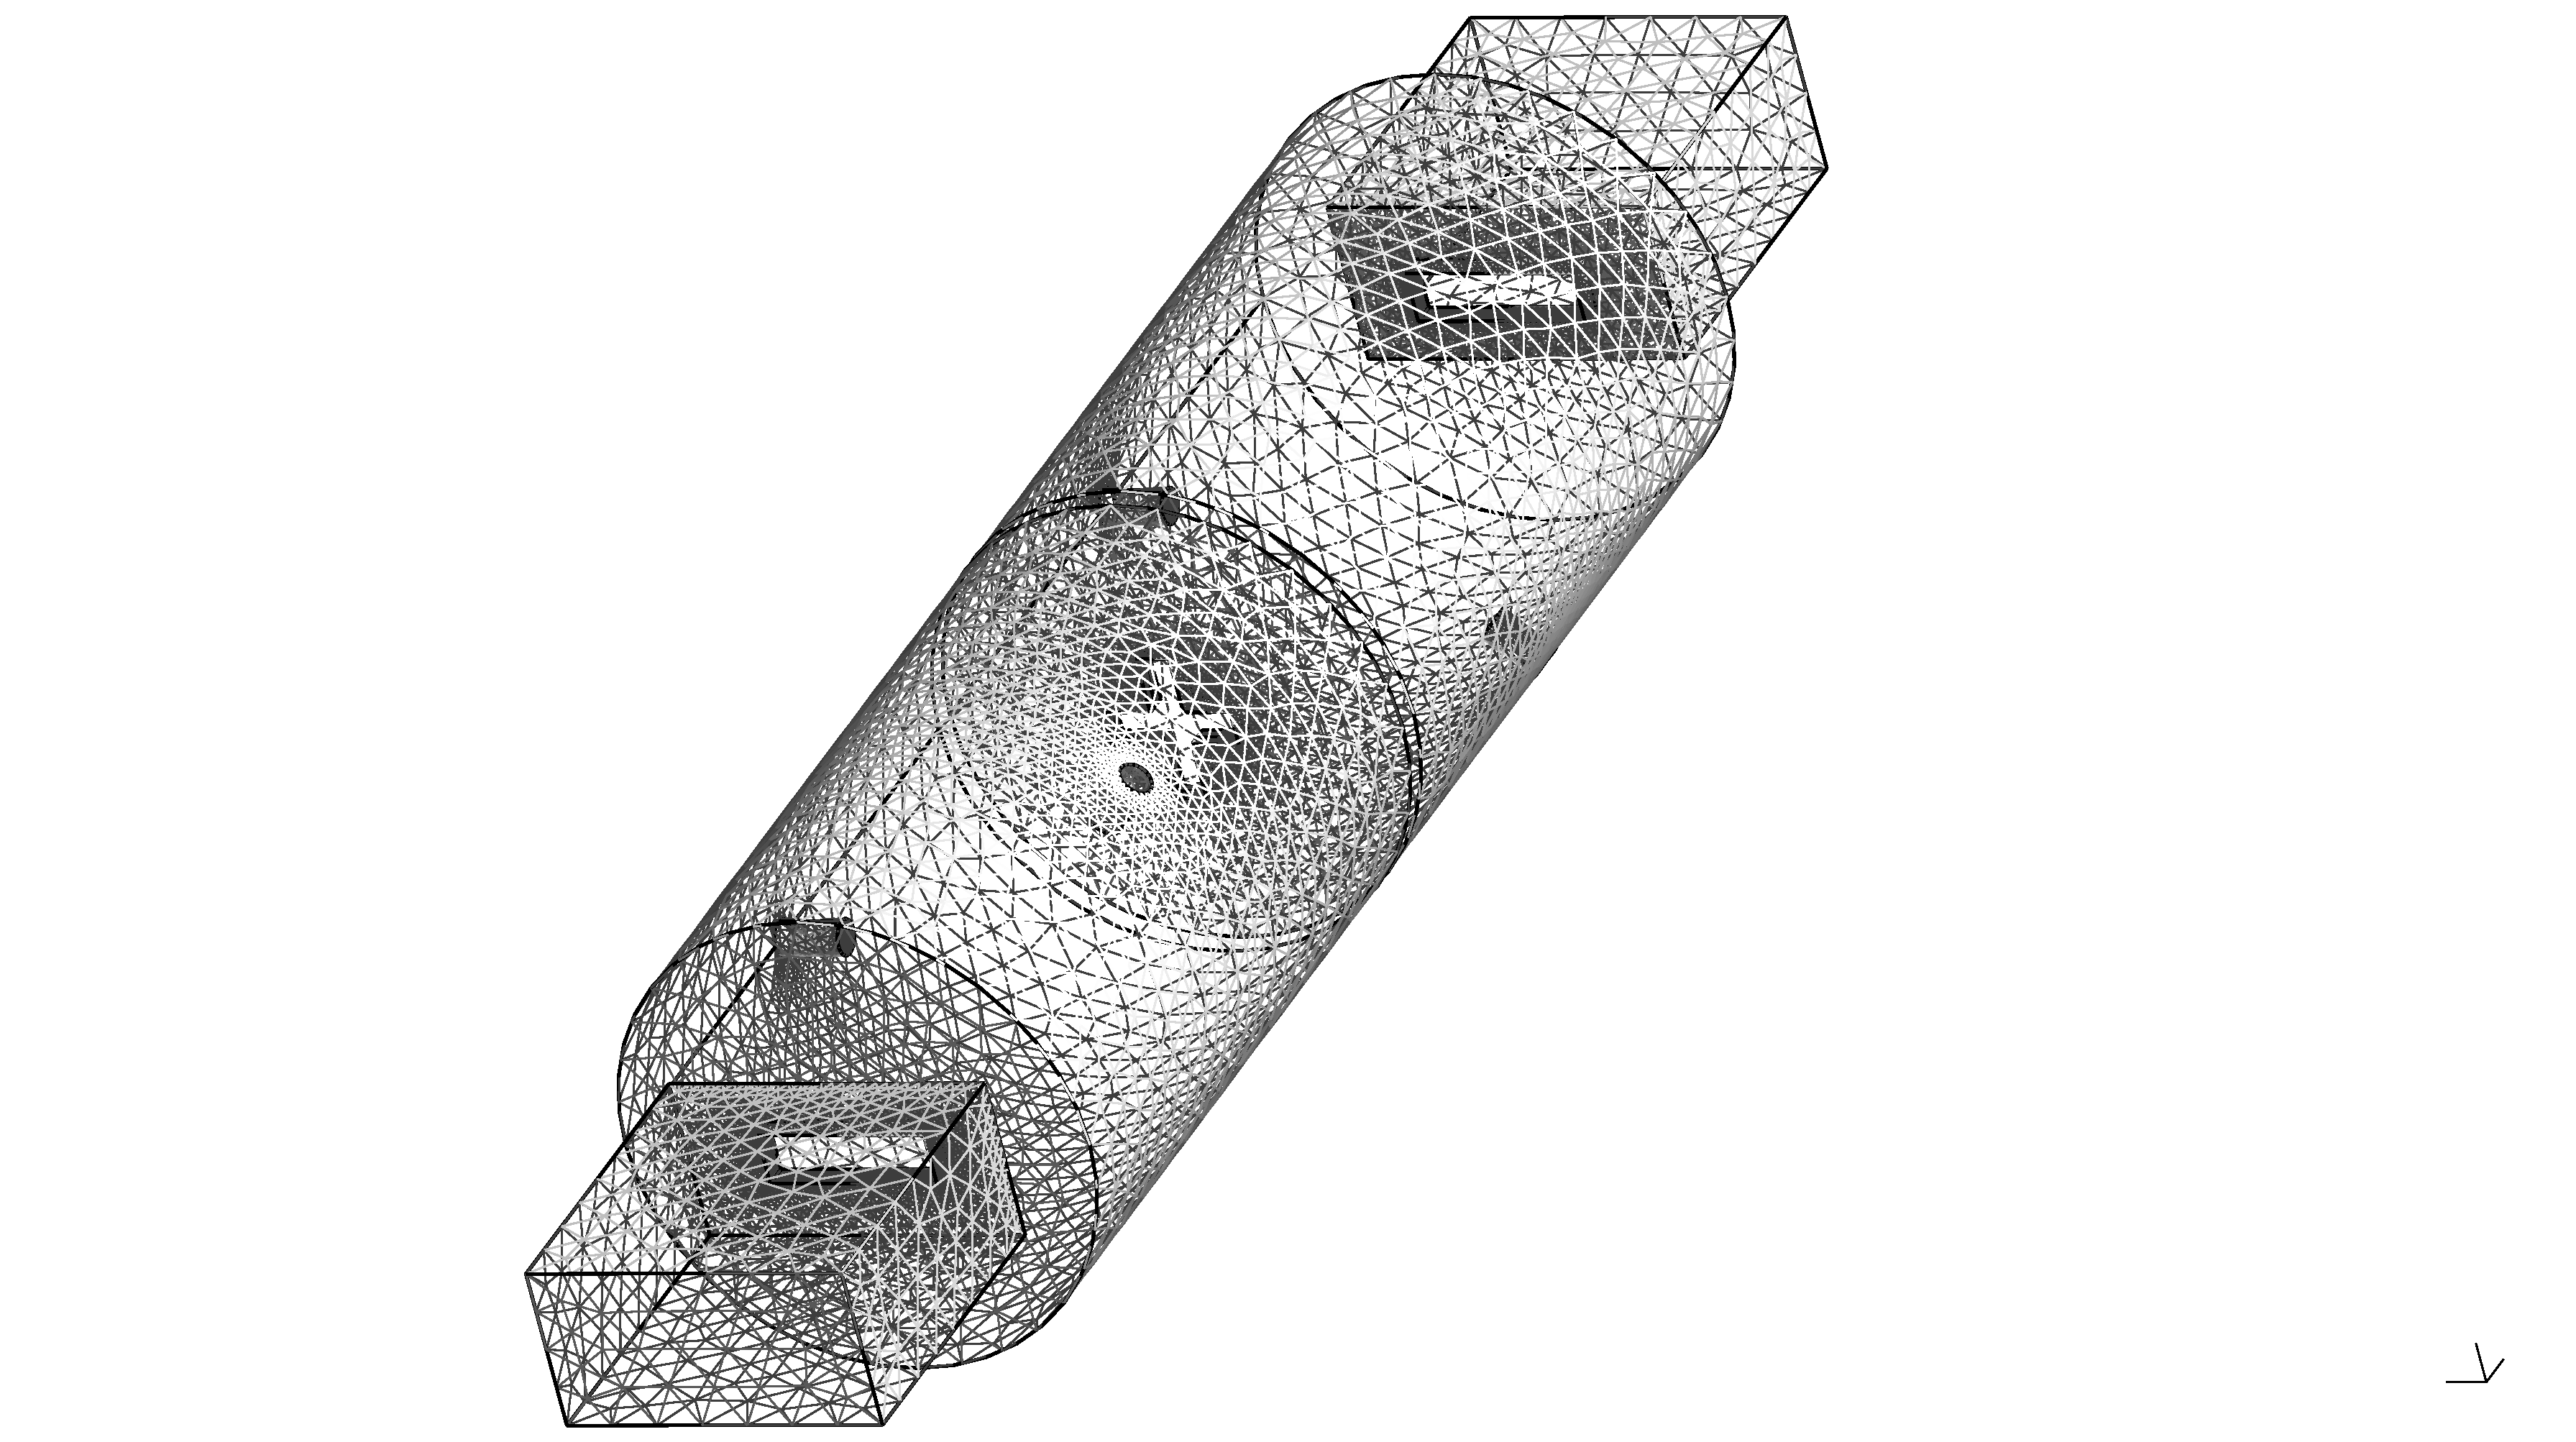
\includegraphics[scale=0.18, trim=12cm 0.2cm 15cm 0.2cm, clip]{figures/DMCWF_surfacemesh.pdf}};
    %\node at (9.4, 2.5) {\includegraphics[scale=0.087]{DMCWF_top.pdf}};
    \draw[thick, fill=black!5!white] (5.65, 1.9) rectangle (6.9, 3.1);
\draw[thick, fill=black!5!white] (7, 1.6) rectangle (9.75, 3.4);
\draw[thick, fill=black!5!white] (9.85, 1.6) rectangle (12.65, 3.4);
\draw[thick, fill=black!5!white] (12.75, 1.9) rectangle (14, 3.1);
\draw[thick] (6.9, 2.15) to (7, 2.15);
\draw[thick] (6.9, 2.85) to (7, 2.85);
\draw[thick] (12.65, 2.15) to (12.75, 2.15);
\draw[thick] (12.65, 2.85) to (12.75, 2.85);
\draw[thick] (9.75, 2.25) to (9.85, 2.25);
\draw[thick] (9.75, 2.75) to (9.85, 2.75);
\draw[thick] (8.37, 1.85) ellipse (0.07 and 0.04);
\draw[thick, opacity=0.2] (11.25, 1.85) ellipse (0.07 and 0.04);
\draw[thick] (8.29, 3.375) to (8.44, 3.375);
\draw[thick] (11.17, 3.375) to (11.33, 3.375);

\draw[<->] (7, 3.6) -- (9.75, 3.6) node [midway, above] {$L_C$};
\draw[<->] (5.65, 3.3) -- (6.9, 3.3) node [midway, above] {$L_B$};
\draw[<->] (5.45, 3.1) -- (5.45, 1.9) node [midway, left] {$W_B$};
\draw[<->] (7.8, 1.7) -- (7.8, 3.3) node [midway, left] {$D_C$};

\begin{scope}[shift={(0, -0.5)}]

    \draw[thick, fill=black!5!white] (6.5, 0) circle (1);
    \draw[thick, fill=black!10!white] (5.8, -0.35) rectangle (7.2, 0.35);
    \draw[thick, fill=white] (6.1, -0.083) rectangle (6.9, 0.083);

    \draw[dashed] (6.1, 0.083) to (6.1, 1.25);
    \draw[dashed] (6.9, 0.083) to (6.9, 1.25);
    \draw[<->] (6.1, 1.15) -- (6.9, 1.15) node [midway, above] {$W_S$};
    \draw[dashed] (6.1, 0.083) to (5.2, 0.083);
    \draw[dashed] (6.1, -0.083) to (5.2, -0.083);
    \draw[<->] (5.3, -0.083) -- (5.3, 0.083) node [midway, left] {$H_S$};
    \draw[dashed] (7.2, -0.35) to (7.7, -0.35);
    \draw[dashed] (7.2, 0.35) to (7.7, 0.35);
    \draw[<->] (7.6, -0.35) -- (7.6, 0.35) node [midway, right] {$H_B$};

\end{scope}

\begin{scope}[shift={(0.05, -0.5)}]

    \draw[thick, fill=black!5!white] (9.76, 0) circle (1);
    \draw[thick, fill=white] (9.68, -0.35) to (9.84, -0.35) to (9.84, -0.08) to (10.06, -0.08)
                    to (10.06, 0.08) to (9.84, 0.08) to (9.84, 0.35) to (9.68, 0.35)
                    to (9.68, 0.08) to (9.46, 0.08) to (9.46, -0.08) to (9.68, -0.08)
                    to cycle;


    \draw[dashed] (9.84, 0.35) to (9.84, 1.25);
    \draw[dashed] (9.68, 0.35) to (9.68, 1.25);
    \draw[<->] (9.68, 1.15) -- (9.84, 1.15) node [midway, above] {$W_A$};
    
    \draw[dashed] (9.68, -0.35) to (9.68, -1.25);
    \draw[dashed] (9.46, -0.083) to (9.46, -1.25);
    \draw[<->] (9.46, -1.15) -- (9.68, -1.15) node [midway, below] {$L_A$};

    %\draw[dashed] (9.46, -0.083) to (8.5, -0.083);
    %\draw[dashed] (9.46, 0.083) to (8.5, 0.083);
    %\draw[<->] (8.6, -0.083) -- (8.6, 0.083) node [midway, left] {$c$};
    
    \draw[dashed] (9.84, 0.35) to (11, 0.35);
    \draw[dashed] (10.06, 0.083) to (11, 0.083);
    \draw[<->] (10.9, 0.083) -- (10.9, 0.35) node [midway, right] {$H_A$};

\end{scope}
\end{tikzpicture}
    \caption{The surface-mesh of the modelled dual-mode circular waveguide filter
    (left). An effort was made to keep the dimensions as similar to the ones
    given in \cite{DMCWF-Dimensions}, but a full correspondence cannot be guaranteed
    due to yours truly being unable to resolve certain ambiguities that were encountered.
    The model adheres to the following dimensions:
    $W_C=43.87$ mm, $D_C=28.0$ mm, $L_B=43.87$ mm, $W_B=19.05$ mm, $H_B=9.525$ mm,
    $L_B=20.0$ mm, $W_S=10.05$ mm, $H_S=3.0$ mm, $W_A=2.0$ mm, $H_A=3.375$ mm,
    $L_A=2.825$ mm; The thickness of all irises is $2.0$ mm; The screws
    are placed exactly half way up the two resonant cylinders,
    with the horizontal tuning screws reaching a depth of $3.82$ mm into the cavity
    and coupling screws at angles $\pm 45^{\circ}$ with a depth of $3.57$ mm.
    Observe that the \acrshort{DMCWF} is point symmetric with respect to the center 
    of the cross iris.}
    \label{fig:DMCWF}
\end{figure}

% Modeling process cite rubia
I created the model in the computer-aided design modeler software application
FreeCAD\footnote{\url{https://www.freecadweb.org/}}. The mesh was defined using 
the 3D finite element mesh generator Gmsh\footnote{\url{https://gmsh.info/}} and 
is available for download on the git repository 
of this project \cite{git}. In Gmsh, a element size factor of 0.2 and 5 smoothing steps
are used for the Delaunay 3D meshing algorithm. Additionally, 
the mesh was refined around critical components such as the screws and irises
using transfinite curves (the sharp-eyed reader may observe these refinements
in the surface mesh visualized in Figure \ref{fig:DMCWF}). A total of
185726 \acrshort{DOF}s are accounted for. The conversion of the
mesh to the FEniCS supported .xml format was performed with the mesh format converter
meshio\footnote{\url{https://github.com/nschloe/meshio}}. 

% Scattering coefficient
In the following, I would like to demonstrate the capability of the 
\acrshort{gMRI} algorithm to approximate scattering coefficients for the \acrshort{DMCWF}.
The definition of the scattering matrix is a adaptation from \cite{shortMRI} to
\begin{equation}
    \mathbf{\underline{S}}(\omega) = \mathbf{\underline{1}}
    - 2\left( \mathbf{\underline{1}} + i \frac{\omega}{2\pi} \sqrt{\frac{\mu}{\epsilon}}
    \sqrt{\frac{1 - (\omega_c / \omega_0)^2}{1 - (\omega_c / \omega)^2}} 
    \mathbf{\underline{F}}^H \mathbf{\underline{U}}(\omega) \right)^{-1}
\end{equation}
where $\mathbf{\underline{F}} = [\mathbf{f}_1, \mathbf{f}_2]$ and
$\mathbf{\underline{U}} = [\mathbf{u}_1, \mathbf{u}_2]$ with $\mathbf{f}_1$ the source term
resulting when the \acrshort{DMCWF} is forced from one side, producing the
solution $\mathbf{u}_1$, and the $\mathbf{f}_2$ when forcing from the other side to
produce $\mathbf{u}_2$. $\omega_c = 4.122 \times 10^{10}$ and $\omega_0 = 6.283 \times 10^{10}$
were assumed. The scattering coefficients $S_{ij}$ are then precisely the
entries of the scattering matrix
\begin{equation}
    \mathbf{\underline{S}}(\omega) =
    \begin{bmatrix}
            S_{11}(\omega) & S_{12}(\omega) \\
            S_{21}(\omega) & S_{22}(\omega)
    \end{bmatrix}\label{equ:scattering-coefficients}
\end{equation}

For the simulation, $\epsilon = 4 \pi \times 10^{-7}$ and 
$\mu = 8.854187 \times 10^{-12}$ were assumed. The one-sided forcing
was performed with $\left.\mathbf{g}\right|_{\Gamma_i} = - \mathbf{e}_z$ from the
left-hand inlet, and $\left.\mathbf{g}\right|_{\Gamma_i} = \mathbf{e}_z$ from the
right-hand inlet. The scattering coefficients $S_{11}(\omega)$ and $S_{12}(\omega)$
once computed by using the solutions at 150 uniformly spaced sample frequencies
directly obtained with the \acrshort{FEM},
and once from the rational surrogate computed with \acrshort{gMRI} at a tolerance
of $\tau = 10^{-2}$. Both are shown (but only one is seen) in Figure
\ref{fig:circular-waveguide-scattering}. At somewhat more than four minutes,
the \acrshort{gMRI} was able to deliver the approximated scattering coefficients
roughly 25 times faster than the \acrshort{FEM}. Compared to \cite{DMCWF-FrequencySweep},
the passband is shifted to a slightly lower frequency.

\begin{figure}[ht]
    \centering
    %% Creator: Matplotlib, PGF backend
%%
%% To include the figure in your LaTeX document, write
%%   \input{<filename>.pgf}
%%
%% Make sure the required packages are loaded in your preamble
%%   \usepackage{pgf}
%%
%% Also ensure that all the required font packages are loaded; for instance,
%% the lmodern package is sometimes necessary when using math font.
%%   \usepackage{lmodern}
%%
%% Figures using additional raster images can only be included by \input if
%% they are in the same directory as the main LaTeX file. For loading figures
%% from other directories you can use the `import` package
%%   \usepackage{import}
%%
%% and then include the figures with
%%   \import{<path to file>}{<filename>.pgf}
%%
%% Matplotlib used the following preamble
%%   \usepackage{fontspec}
%%   \setmainfont{DejaVuSans.ttf}[Path=\detokenize{C:/Users/Fabio/Anaconda3/Lib/site-packages/matplotlib/mpl-data/fonts/ttf/}]
%%   \setsansfont{DejaVuSans.ttf}[Path=\detokenize{C:/Users/Fabio/Anaconda3/Lib/site-packages/matplotlib/mpl-data/fonts/ttf/}]
%%   \setmonofont{DejaVuSansMono.ttf}[Path=\detokenize{C:/Users/Fabio/Anaconda3/Lib/site-packages/matplotlib/mpl-data/fonts/ttf/}]
%%
\begingroup%
\makeatletter%
\begin{pgfpicture}%
\pgfpathrectangle{\pgfpointorigin}{\pgfqpoint{5.078495in}{3.668486in}}%
\pgfusepath{use as bounding box, clip}%
\begin{pgfscope}%
\pgfsetbuttcap%
\pgfsetmiterjoin%
\pgfsetlinewidth{0.000000pt}%
\definecolor{currentstroke}{rgb}{1.000000,1.000000,1.000000}%
\pgfsetstrokecolor{currentstroke}%
\pgfsetstrokeopacity{0.000000}%
\pgfsetdash{}{0pt}%
\pgfpathmoveto{\pgfqpoint{0.000000in}{0.000000in}}%
\pgfpathlineto{\pgfqpoint{5.078495in}{0.000000in}}%
\pgfpathlineto{\pgfqpoint{5.078495in}{3.668486in}}%
\pgfpathlineto{\pgfqpoint{0.000000in}{3.668486in}}%
\pgfpathlineto{\pgfqpoint{0.000000in}{0.000000in}}%
\pgfpathclose%
\pgfusepath{}%
\end{pgfscope}%
\begin{pgfscope}%
\pgfsetbuttcap%
\pgfsetmiterjoin%
\definecolor{currentfill}{rgb}{1.000000,1.000000,1.000000}%
\pgfsetfillcolor{currentfill}%
\pgfsetlinewidth{0.000000pt}%
\definecolor{currentstroke}{rgb}{0.000000,0.000000,0.000000}%
\pgfsetstrokecolor{currentstroke}%
\pgfsetstrokeopacity{0.000000}%
\pgfsetdash{}{0pt}%
\pgfpathmoveto{\pgfqpoint{0.677245in}{2.058486in}}%
\pgfpathlineto{\pgfqpoint{4.978495in}{2.058486in}}%
\pgfpathlineto{\pgfqpoint{4.978495in}{3.568486in}}%
\pgfpathlineto{\pgfqpoint{0.677245in}{3.568486in}}%
\pgfpathlineto{\pgfqpoint{0.677245in}{2.058486in}}%
\pgfpathclose%
\pgfusepath{fill}%
\end{pgfscope}%
\begin{pgfscope}%
\pgfsetbuttcap%
\pgfsetroundjoin%
\definecolor{currentfill}{rgb}{0.000000,0.000000,0.000000}%
\pgfsetfillcolor{currentfill}%
\pgfsetlinewidth{0.803000pt}%
\definecolor{currentstroke}{rgb}{0.000000,0.000000,0.000000}%
\pgfsetstrokecolor{currentstroke}%
\pgfsetdash{}{0pt}%
\pgfsys@defobject{currentmarker}{\pgfqpoint{0.000000in}{-0.048611in}}{\pgfqpoint{0.000000in}{0.000000in}}{%
\pgfpathmoveto{\pgfqpoint{0.000000in}{0.000000in}}%
\pgfpathlineto{\pgfqpoint{0.000000in}{-0.048611in}}%
\pgfusepath{stroke,fill}%
}%
\begin{pgfscope}%
\pgfsys@transformshift{1.411800in}{2.058486in}%
\pgfsys@useobject{currentmarker}{}%
\end{pgfscope}%
\end{pgfscope}%
\begin{pgfscope}%
\pgfsetbuttcap%
\pgfsetroundjoin%
\definecolor{currentfill}{rgb}{0.000000,0.000000,0.000000}%
\pgfsetfillcolor{currentfill}%
\pgfsetlinewidth{0.803000pt}%
\definecolor{currentstroke}{rgb}{0.000000,0.000000,0.000000}%
\pgfsetstrokecolor{currentstroke}%
\pgfsetdash{}{0pt}%
\pgfsys@defobject{currentmarker}{\pgfqpoint{0.000000in}{-0.048611in}}{\pgfqpoint{0.000000in}{0.000000in}}{%
\pgfpathmoveto{\pgfqpoint{0.000000in}{0.000000in}}%
\pgfpathlineto{\pgfqpoint{0.000000in}{-0.048611in}}%
\pgfusepath{stroke,fill}%
}%
\begin{pgfscope}%
\pgfsys@transformshift{2.267506in}{2.058486in}%
\pgfsys@useobject{currentmarker}{}%
\end{pgfscope}%
\end{pgfscope}%
\begin{pgfscope}%
\pgfsetbuttcap%
\pgfsetroundjoin%
\definecolor{currentfill}{rgb}{0.000000,0.000000,0.000000}%
\pgfsetfillcolor{currentfill}%
\pgfsetlinewidth{0.803000pt}%
\definecolor{currentstroke}{rgb}{0.000000,0.000000,0.000000}%
\pgfsetstrokecolor{currentstroke}%
\pgfsetdash{}{0pt}%
\pgfsys@defobject{currentmarker}{\pgfqpoint{0.000000in}{-0.048611in}}{\pgfqpoint{0.000000in}{0.000000in}}{%
\pgfpathmoveto{\pgfqpoint{0.000000in}{0.000000in}}%
\pgfpathlineto{\pgfqpoint{0.000000in}{-0.048611in}}%
\pgfusepath{stroke,fill}%
}%
\begin{pgfscope}%
\pgfsys@transformshift{3.123213in}{2.058486in}%
\pgfsys@useobject{currentmarker}{}%
\end{pgfscope}%
\end{pgfscope}%
\begin{pgfscope}%
\pgfsetbuttcap%
\pgfsetroundjoin%
\definecolor{currentfill}{rgb}{0.000000,0.000000,0.000000}%
\pgfsetfillcolor{currentfill}%
\pgfsetlinewidth{0.803000pt}%
\definecolor{currentstroke}{rgb}{0.000000,0.000000,0.000000}%
\pgfsetstrokecolor{currentstroke}%
\pgfsetdash{}{0pt}%
\pgfsys@defobject{currentmarker}{\pgfqpoint{0.000000in}{-0.048611in}}{\pgfqpoint{0.000000in}{0.000000in}}{%
\pgfpathmoveto{\pgfqpoint{0.000000in}{0.000000in}}%
\pgfpathlineto{\pgfqpoint{0.000000in}{-0.048611in}}%
\pgfusepath{stroke,fill}%
}%
\begin{pgfscope}%
\pgfsys@transformshift{3.978919in}{2.058486in}%
\pgfsys@useobject{currentmarker}{}%
\end{pgfscope}%
\end{pgfscope}%
\begin{pgfscope}%
\pgfsetbuttcap%
\pgfsetroundjoin%
\definecolor{currentfill}{rgb}{0.000000,0.000000,0.000000}%
\pgfsetfillcolor{currentfill}%
\pgfsetlinewidth{0.803000pt}%
\definecolor{currentstroke}{rgb}{0.000000,0.000000,0.000000}%
\pgfsetstrokecolor{currentstroke}%
\pgfsetdash{}{0pt}%
\pgfsys@defobject{currentmarker}{\pgfqpoint{0.000000in}{-0.048611in}}{\pgfqpoint{0.000000in}{0.000000in}}{%
\pgfpathmoveto{\pgfqpoint{0.000000in}{0.000000in}}%
\pgfpathlineto{\pgfqpoint{0.000000in}{-0.048611in}}%
\pgfusepath{stroke,fill}%
}%
\begin{pgfscope}%
\pgfsys@transformshift{4.834626in}{2.058486in}%
\pgfsys@useobject{currentmarker}{}%
\end{pgfscope}%
\end{pgfscope}%
\begin{pgfscope}%
\pgfpathrectangle{\pgfqpoint{0.677245in}{2.058486in}}{\pgfqpoint{4.301250in}{1.510000in}}%
\pgfusepath{clip}%
\pgfsetrectcap%
\pgfsetroundjoin%
\pgfsetlinewidth{0.803000pt}%
\definecolor{currentstroke}{rgb}{0.690196,0.690196,0.690196}%
\pgfsetstrokecolor{currentstroke}%
\pgfsetdash{}{0pt}%
\pgfpathmoveto{\pgfqpoint{0.677245in}{2.416736in}}%
\pgfpathlineto{\pgfqpoint{4.978495in}{2.416736in}}%
\pgfusepath{stroke}%
\end{pgfscope}%
\begin{pgfscope}%
\pgfsetbuttcap%
\pgfsetroundjoin%
\definecolor{currentfill}{rgb}{0.000000,0.000000,0.000000}%
\pgfsetfillcolor{currentfill}%
\pgfsetlinewidth{0.803000pt}%
\definecolor{currentstroke}{rgb}{0.000000,0.000000,0.000000}%
\pgfsetstrokecolor{currentstroke}%
\pgfsetdash{}{0pt}%
\pgfsys@defobject{currentmarker}{\pgfqpoint{-0.048611in}{0.000000in}}{\pgfqpoint{-0.000000in}{0.000000in}}{%
\pgfpathmoveto{\pgfqpoint{-0.000000in}{0.000000in}}%
\pgfpathlineto{\pgfqpoint{-0.048611in}{0.000000in}}%
\pgfusepath{stroke,fill}%
}%
\begin{pgfscope}%
\pgfsys@transformshift{0.677245in}{2.416736in}%
\pgfsys@useobject{currentmarker}{}%
\end{pgfscope}%
\end{pgfscope}%
\begin{pgfscope}%
\definecolor{textcolor}{rgb}{0.000000,0.000000,0.000000}%
\pgfsetstrokecolor{textcolor}%
\pgfsetfillcolor{textcolor}%
\pgftext[x=0.309652in, y=2.358699in, left, base]{\color{textcolor}\rmfamily\fontsize{11.000000}{13.200000}\selectfont \(\displaystyle {\ensuremath{-}40}\)}%
\end{pgfscope}%
\begin{pgfscope}%
\pgfpathrectangle{\pgfqpoint{0.677245in}{2.058486in}}{\pgfqpoint{4.301250in}{1.510000in}}%
\pgfusepath{clip}%
\pgfsetrectcap%
\pgfsetroundjoin%
\pgfsetlinewidth{0.803000pt}%
\definecolor{currentstroke}{rgb}{0.690196,0.690196,0.690196}%
\pgfsetstrokecolor{currentstroke}%
\pgfsetdash{}{0pt}%
\pgfpathmoveto{\pgfqpoint{0.677245in}{2.958293in}}%
\pgfpathlineto{\pgfqpoint{4.978495in}{2.958293in}}%
\pgfusepath{stroke}%
\end{pgfscope}%
\begin{pgfscope}%
\pgfsetbuttcap%
\pgfsetroundjoin%
\definecolor{currentfill}{rgb}{0.000000,0.000000,0.000000}%
\pgfsetfillcolor{currentfill}%
\pgfsetlinewidth{0.803000pt}%
\definecolor{currentstroke}{rgb}{0.000000,0.000000,0.000000}%
\pgfsetstrokecolor{currentstroke}%
\pgfsetdash{}{0pt}%
\pgfsys@defobject{currentmarker}{\pgfqpoint{-0.048611in}{0.000000in}}{\pgfqpoint{-0.000000in}{0.000000in}}{%
\pgfpathmoveto{\pgfqpoint{-0.000000in}{0.000000in}}%
\pgfpathlineto{\pgfqpoint{-0.048611in}{0.000000in}}%
\pgfusepath{stroke,fill}%
}%
\begin{pgfscope}%
\pgfsys@transformshift{0.677245in}{2.958293in}%
\pgfsys@useobject{currentmarker}{}%
\end{pgfscope}%
\end{pgfscope}%
\begin{pgfscope}%
\definecolor{textcolor}{rgb}{0.000000,0.000000,0.000000}%
\pgfsetstrokecolor{textcolor}%
\pgfsetfillcolor{textcolor}%
\pgftext[x=0.309652in, y=2.900255in, left, base]{\color{textcolor}\rmfamily\fontsize{11.000000}{13.200000}\selectfont \(\displaystyle {\ensuremath{-}20}\)}%
\end{pgfscope}%
\begin{pgfscope}%
\pgfpathrectangle{\pgfqpoint{0.677245in}{2.058486in}}{\pgfqpoint{4.301250in}{1.510000in}}%
\pgfusepath{clip}%
\pgfsetrectcap%
\pgfsetroundjoin%
\pgfsetlinewidth{0.803000pt}%
\definecolor{currentstroke}{rgb}{0.690196,0.690196,0.690196}%
\pgfsetstrokecolor{currentstroke}%
\pgfsetdash{}{0pt}%
\pgfpathmoveto{\pgfqpoint{0.677245in}{3.499849in}}%
\pgfpathlineto{\pgfqpoint{4.978495in}{3.499849in}}%
\pgfusepath{stroke}%
\end{pgfscope}%
\begin{pgfscope}%
\pgfsetbuttcap%
\pgfsetroundjoin%
\definecolor{currentfill}{rgb}{0.000000,0.000000,0.000000}%
\pgfsetfillcolor{currentfill}%
\pgfsetlinewidth{0.803000pt}%
\definecolor{currentstroke}{rgb}{0.000000,0.000000,0.000000}%
\pgfsetstrokecolor{currentstroke}%
\pgfsetdash{}{0pt}%
\pgfsys@defobject{currentmarker}{\pgfqpoint{-0.048611in}{0.000000in}}{\pgfqpoint{-0.000000in}{0.000000in}}{%
\pgfpathmoveto{\pgfqpoint{-0.000000in}{0.000000in}}%
\pgfpathlineto{\pgfqpoint{-0.048611in}{0.000000in}}%
\pgfusepath{stroke,fill}%
}%
\begin{pgfscope}%
\pgfsys@transformshift{0.677245in}{3.499849in}%
\pgfsys@useobject{currentmarker}{}%
\end{pgfscope}%
\end{pgfscope}%
\begin{pgfscope}%
\definecolor{textcolor}{rgb}{0.000000,0.000000,0.000000}%
\pgfsetstrokecolor{textcolor}%
\pgfsetfillcolor{textcolor}%
\pgftext[x=0.503981in, y=3.441812in, left, base]{\color{textcolor}\rmfamily\fontsize{11.000000}{13.200000}\selectfont \(\displaystyle {0}\)}%
\end{pgfscope}%
\begin{pgfscope}%
\definecolor{textcolor}{rgb}{0.000000,0.000000,0.000000}%
\pgfsetstrokecolor{textcolor}%
\pgfsetfillcolor{textcolor}%
\pgftext[x=0.254096in,y=2.813486in,,bottom,rotate=90.000000]{\color{textcolor}\rmfamily\fontsize{11.000000}{13.200000}\selectfont \(\displaystyle S_{11}(\omega)\) (dB)}%
\end{pgfscope}%
\begin{pgfscope}%
\pgfpathrectangle{\pgfqpoint{0.677245in}{2.058486in}}{\pgfqpoint{4.301250in}{1.510000in}}%
\pgfusepath{clip}%
\pgfsetrectcap%
\pgfsetroundjoin%
\pgfsetlinewidth{1.505625pt}%
\definecolor{currentstroke}{rgb}{0.001462,0.000466,0.013866}%
\pgfsetstrokecolor{currentstroke}%
\pgfsetdash{}{0pt}%
\pgfpathmoveto{\pgfqpoint{0.677245in}{3.498630in}}%
\pgfpathlineto{\pgfqpoint{1.803075in}{3.496865in}}%
\pgfpathlineto{\pgfqpoint{1.976280in}{3.499849in}}%
\pgfpathlineto{\pgfqpoint{2.034015in}{3.497600in}}%
\pgfpathlineto{\pgfqpoint{2.062882in}{3.493945in}}%
\pgfpathlineto{\pgfqpoint{2.091750in}{3.486979in}}%
\pgfpathlineto{\pgfqpoint{2.120617in}{3.474489in}}%
\pgfpathlineto{\pgfqpoint{2.149485in}{3.452864in}}%
\pgfpathlineto{\pgfqpoint{2.178352in}{3.416462in}}%
\pgfpathlineto{\pgfqpoint{2.207219in}{3.356865in}}%
\pgfpathlineto{\pgfqpoint{2.236087in}{3.262664in}}%
\pgfpathlineto{\pgfqpoint{2.264954in}{3.118970in}}%
\pgfpathlineto{\pgfqpoint{2.293822in}{2.904230in}}%
\pgfpathlineto{\pgfqpoint{2.322689in}{2.574688in}}%
\pgfpathlineto{\pgfqpoint{2.351557in}{2.127122in}}%
\pgfpathlineto{\pgfqpoint{2.380424in}{2.353954in}}%
\pgfpathlineto{\pgfqpoint{2.409292in}{2.635869in}}%
\pgfpathlineto{\pgfqpoint{2.438159in}{2.797759in}}%
\pgfpathlineto{\pgfqpoint{2.467026in}{2.900111in}}%
\pgfpathlineto{\pgfqpoint{2.495894in}{2.969325in}}%
\pgfpathlineto{\pgfqpoint{2.524761in}{3.018407in}}%
\pgfpathlineto{\pgfqpoint{2.553629in}{3.053946in}}%
\pgfpathlineto{\pgfqpoint{2.582496in}{3.080155in}}%
\pgfpathlineto{\pgfqpoint{2.611364in}{3.099255in}}%
\pgfpathlineto{\pgfqpoint{2.640231in}{3.113016in}}%
\pgfpathlineto{\pgfqpoint{2.669099in}{3.122227in}}%
\pgfpathlineto{\pgfqpoint{2.697966in}{3.127715in}}%
\pgfpathlineto{\pgfqpoint{2.726834in}{3.129637in}}%
\pgfpathlineto{\pgfqpoint{2.755701in}{3.128331in}}%
\pgfpathlineto{\pgfqpoint{2.784568in}{3.123556in}}%
\pgfpathlineto{\pgfqpoint{2.813436in}{3.115261in}}%
\pgfpathlineto{\pgfqpoint{2.842303in}{3.102796in}}%
\pgfpathlineto{\pgfqpoint{2.871171in}{3.085606in}}%
\pgfpathlineto{\pgfqpoint{2.900038in}{3.062380in}}%
\pgfpathlineto{\pgfqpoint{2.928906in}{3.031606in}}%
\pgfpathlineto{\pgfqpoint{2.957773in}{2.990527in}}%
\pgfpathlineto{\pgfqpoint{2.986641in}{2.935315in}}%
\pgfpathlineto{\pgfqpoint{3.015508in}{2.859337in}}%
\pgfpathlineto{\pgfqpoint{3.044375in}{2.752175in}}%
\pgfpathlineto{\pgfqpoint{3.073243in}{2.598180in}}%
\pgfpathlineto{\pgfqpoint{3.102110in}{2.406507in}}%
\pgfpathlineto{\pgfqpoint{3.130978in}{2.403647in}}%
\pgfpathlineto{\pgfqpoint{3.159845in}{2.665074in}}%
\pgfpathlineto{\pgfqpoint{3.188713in}{2.906353in}}%
\pgfpathlineto{\pgfqpoint{3.217580in}{3.085759in}}%
\pgfpathlineto{\pgfqpoint{3.246448in}{3.215996in}}%
\pgfpathlineto{\pgfqpoint{3.275315in}{3.308939in}}%
\pgfpathlineto{\pgfqpoint{3.304183in}{3.373705in}}%
\pgfpathlineto{\pgfqpoint{3.333050in}{3.417910in}}%
\pgfpathlineto{\pgfqpoint{3.361917in}{3.447524in}}%
\pgfpathlineto{\pgfqpoint{3.390785in}{3.467123in}}%
\pgfpathlineto{\pgfqpoint{3.419652in}{3.479931in}}%
\pgfpathlineto{\pgfqpoint{3.448520in}{3.488200in}}%
\pgfpathlineto{\pgfqpoint{3.477387in}{3.493434in}}%
\pgfpathlineto{\pgfqpoint{3.535122in}{3.498510in}}%
\pgfpathlineto{\pgfqpoint{3.592857in}{3.499844in}}%
\pgfpathlineto{\pgfqpoint{3.708327in}{3.498590in}}%
\pgfpathlineto{\pgfqpoint{4.083604in}{3.492401in}}%
\pgfpathlineto{\pgfqpoint{4.430013in}{3.490532in}}%
\pgfpathlineto{\pgfqpoint{4.978495in}{3.491037in}}%
\pgfpathlineto{\pgfqpoint{4.978495in}{3.491037in}}%
\pgfusepath{stroke}%
\end{pgfscope}%
\begin{pgfscope}%
\pgfpathrectangle{\pgfqpoint{0.677245in}{2.058486in}}{\pgfqpoint{4.301250in}{1.510000in}}%
\pgfusepath{clip}%
\pgfsetrectcap%
\pgfsetroundjoin%
\pgfsetlinewidth{1.505625pt}%
\definecolor{currentstroke}{rgb}{0.735683,0.215906,0.330245}%
\pgfsetstrokecolor{currentstroke}%
\pgfsetdash{}{0pt}%
\pgfpathmoveto{\pgfqpoint{0.677245in}{3.498630in}}%
\pgfpathlineto{\pgfqpoint{1.803075in}{3.496865in}}%
\pgfpathlineto{\pgfqpoint{1.976280in}{3.499849in}}%
\pgfpathlineto{\pgfqpoint{2.034015in}{3.497600in}}%
\pgfpathlineto{\pgfqpoint{2.062882in}{3.493945in}}%
\pgfpathlineto{\pgfqpoint{2.091750in}{3.486979in}}%
\pgfpathlineto{\pgfqpoint{2.120617in}{3.474489in}}%
\pgfpathlineto{\pgfqpoint{2.149485in}{3.452864in}}%
\pgfpathlineto{\pgfqpoint{2.178352in}{3.416462in}}%
\pgfpathlineto{\pgfqpoint{2.207219in}{3.356865in}}%
\pgfpathlineto{\pgfqpoint{2.236087in}{3.262663in}}%
\pgfpathlineto{\pgfqpoint{2.264954in}{3.118969in}}%
\pgfpathlineto{\pgfqpoint{2.293822in}{2.904229in}}%
\pgfpathlineto{\pgfqpoint{2.322689in}{2.574685in}}%
\pgfpathlineto{\pgfqpoint{2.351557in}{2.127122in}}%
\pgfpathlineto{\pgfqpoint{2.380424in}{2.353959in}}%
\pgfpathlineto{\pgfqpoint{2.409292in}{2.635872in}}%
\pgfpathlineto{\pgfqpoint{2.438159in}{2.797761in}}%
\pgfpathlineto{\pgfqpoint{2.467026in}{2.900113in}}%
\pgfpathlineto{\pgfqpoint{2.495894in}{2.969326in}}%
\pgfpathlineto{\pgfqpoint{2.524761in}{3.018408in}}%
\pgfpathlineto{\pgfqpoint{2.553629in}{3.053948in}}%
\pgfpathlineto{\pgfqpoint{2.582496in}{3.080156in}}%
\pgfpathlineto{\pgfqpoint{2.611364in}{3.099256in}}%
\pgfpathlineto{\pgfqpoint{2.640231in}{3.113017in}}%
\pgfpathlineto{\pgfqpoint{2.669099in}{3.122228in}}%
\pgfpathlineto{\pgfqpoint{2.697966in}{3.127716in}}%
\pgfpathlineto{\pgfqpoint{2.726834in}{3.129638in}}%
\pgfpathlineto{\pgfqpoint{2.755701in}{3.128332in}}%
\pgfpathlineto{\pgfqpoint{2.784568in}{3.123557in}}%
\pgfpathlineto{\pgfqpoint{2.813436in}{3.115262in}}%
\pgfpathlineto{\pgfqpoint{2.842303in}{3.102797in}}%
\pgfpathlineto{\pgfqpoint{2.871171in}{3.085607in}}%
\pgfpathlineto{\pgfqpoint{2.900038in}{3.062381in}}%
\pgfpathlineto{\pgfqpoint{2.928906in}{3.031607in}}%
\pgfpathlineto{\pgfqpoint{2.957773in}{2.990528in}}%
\pgfpathlineto{\pgfqpoint{2.986641in}{2.935316in}}%
\pgfpathlineto{\pgfqpoint{3.015508in}{2.859338in}}%
\pgfpathlineto{\pgfqpoint{3.044375in}{2.752175in}}%
\pgfpathlineto{\pgfqpoint{3.073243in}{2.598181in}}%
\pgfpathlineto{\pgfqpoint{3.102110in}{2.406507in}}%
\pgfpathlineto{\pgfqpoint{3.130978in}{2.403647in}}%
\pgfpathlineto{\pgfqpoint{3.159845in}{2.665074in}}%
\pgfpathlineto{\pgfqpoint{3.188713in}{2.906353in}}%
\pgfpathlineto{\pgfqpoint{3.217580in}{3.085759in}}%
\pgfpathlineto{\pgfqpoint{3.246448in}{3.215996in}}%
\pgfpathlineto{\pgfqpoint{3.275315in}{3.308939in}}%
\pgfpathlineto{\pgfqpoint{3.304183in}{3.373705in}}%
\pgfpathlineto{\pgfqpoint{3.333050in}{3.417910in}}%
\pgfpathlineto{\pgfqpoint{3.361917in}{3.447524in}}%
\pgfpathlineto{\pgfqpoint{3.390785in}{3.467123in}}%
\pgfpathlineto{\pgfqpoint{3.419652in}{3.479931in}}%
\pgfpathlineto{\pgfqpoint{3.448520in}{3.488200in}}%
\pgfpathlineto{\pgfqpoint{3.477387in}{3.493434in}}%
\pgfpathlineto{\pgfqpoint{3.535122in}{3.498510in}}%
\pgfpathlineto{\pgfqpoint{3.592857in}{3.499844in}}%
\pgfpathlineto{\pgfqpoint{3.708327in}{3.498590in}}%
\pgfpathlineto{\pgfqpoint{4.083604in}{3.492399in}}%
\pgfpathlineto{\pgfqpoint{4.430013in}{3.490529in}}%
\pgfpathlineto{\pgfqpoint{4.978495in}{3.491037in}}%
\pgfpathlineto{\pgfqpoint{4.978495in}{3.491037in}}%
\pgfusepath{stroke}%
\end{pgfscope}%
\begin{pgfscope}%
\pgfsetrectcap%
\pgfsetmiterjoin%
\pgfsetlinewidth{0.803000pt}%
\definecolor{currentstroke}{rgb}{0.000000,0.000000,0.000000}%
\pgfsetstrokecolor{currentstroke}%
\pgfsetdash{}{0pt}%
\pgfpathmoveto{\pgfqpoint{0.677245in}{2.058486in}}%
\pgfpathlineto{\pgfqpoint{0.677245in}{3.568486in}}%
\pgfusepath{stroke}%
\end{pgfscope}%
\begin{pgfscope}%
\pgfsetrectcap%
\pgfsetmiterjoin%
\pgfsetlinewidth{0.803000pt}%
\definecolor{currentstroke}{rgb}{0.000000,0.000000,0.000000}%
\pgfsetstrokecolor{currentstroke}%
\pgfsetdash{}{0pt}%
\pgfpathmoveto{\pgfqpoint{4.978495in}{2.058486in}}%
\pgfpathlineto{\pgfqpoint{4.978495in}{3.568486in}}%
\pgfusepath{stroke}%
\end{pgfscope}%
\begin{pgfscope}%
\pgfsetrectcap%
\pgfsetmiterjoin%
\pgfsetlinewidth{0.803000pt}%
\definecolor{currentstroke}{rgb}{0.000000,0.000000,0.000000}%
\pgfsetstrokecolor{currentstroke}%
\pgfsetdash{}{0pt}%
\pgfpathmoveto{\pgfqpoint{0.677245in}{2.058486in}}%
\pgfpathlineto{\pgfqpoint{4.978495in}{2.058486in}}%
\pgfusepath{stroke}%
\end{pgfscope}%
\begin{pgfscope}%
\pgfsetrectcap%
\pgfsetmiterjoin%
\pgfsetlinewidth{0.803000pt}%
\definecolor{currentstroke}{rgb}{0.000000,0.000000,0.000000}%
\pgfsetstrokecolor{currentstroke}%
\pgfsetdash{}{0pt}%
\pgfpathmoveto{\pgfqpoint{0.677245in}{3.568486in}}%
\pgfpathlineto{\pgfqpoint{4.978495in}{3.568486in}}%
\pgfusepath{stroke}%
\end{pgfscope}%
\begin{pgfscope}%
\pgfsetbuttcap%
\pgfsetmiterjoin%
\definecolor{currentfill}{rgb}{1.000000,1.000000,1.000000}%
\pgfsetfillcolor{currentfill}%
\pgfsetfillopacity{0.800000}%
\pgfsetlinewidth{1.003750pt}%
\definecolor{currentstroke}{rgb}{0.800000,0.800000,0.800000}%
\pgfsetstrokecolor{currentstroke}%
\pgfsetstrokeopacity{0.800000}%
\pgfsetdash{}{0pt}%
\pgfpathmoveto{\pgfqpoint{3.653162in}{2.134875in}}%
\pgfpathlineto{\pgfqpoint{4.871550in}{2.134875in}}%
\pgfpathquadraticcurveto{\pgfqpoint{4.902106in}{2.134875in}}{\pgfqpoint{4.902106in}{2.165430in}}%
\pgfpathlineto{\pgfqpoint{4.902106in}{2.598638in}}%
\pgfpathquadraticcurveto{\pgfqpoint{4.902106in}{2.629194in}}{\pgfqpoint{4.871550in}{2.629194in}}%
\pgfpathlineto{\pgfqpoint{3.653162in}{2.629194in}}%
\pgfpathquadraticcurveto{\pgfqpoint{3.622607in}{2.629194in}}{\pgfqpoint{3.622607in}{2.598638in}}%
\pgfpathlineto{\pgfqpoint{3.622607in}{2.165430in}}%
\pgfpathquadraticcurveto{\pgfqpoint{3.622607in}{2.134875in}}{\pgfqpoint{3.653162in}{2.134875in}}%
\pgfpathlineto{\pgfqpoint{3.653162in}{2.134875in}}%
\pgfpathclose%
\pgfusepath{stroke,fill}%
\end{pgfscope}%
\begin{pgfscope}%
\pgfsetrectcap%
\pgfsetroundjoin%
\pgfsetlinewidth{1.505625pt}%
\definecolor{currentstroke}{rgb}{0.001462,0.000466,0.013866}%
\pgfsetstrokecolor{currentstroke}%
\pgfsetdash{}{0pt}%
\pgfpathmoveto{\pgfqpoint{3.683718in}{2.505480in}}%
\pgfpathlineto{\pgfqpoint{3.836496in}{2.505480in}}%
\pgfpathlineto{\pgfqpoint{3.989273in}{2.505480in}}%
\pgfusepath{stroke}%
\end{pgfscope}%
\begin{pgfscope}%
\definecolor{textcolor}{rgb}{0.000000,0.000000,0.000000}%
\pgfsetstrokecolor{textcolor}%
\pgfsetfillcolor{textcolor}%
\pgftext[x=4.111496in,y=2.452007in,left,base]{\color{textcolor}\rmfamily\fontsize{11.000000}{13.200000}\selectfont reference}%
\end{pgfscope}%
\begin{pgfscope}%
\pgfsetrectcap%
\pgfsetroundjoin%
\pgfsetlinewidth{1.505625pt}%
\definecolor{currentstroke}{rgb}{0.735683,0.215906,0.330245}%
\pgfsetstrokecolor{currentstroke}%
\pgfsetdash{}{0pt}%
\pgfpathmoveto{\pgfqpoint{3.683718in}{2.281237in}}%
\pgfpathlineto{\pgfqpoint{3.836496in}{2.281237in}}%
\pgfpathlineto{\pgfqpoint{3.989273in}{2.281237in}}%
\pgfusepath{stroke}%
\end{pgfscope}%
\begin{pgfscope}%
\definecolor{textcolor}{rgb}{0.000000,0.000000,0.000000}%
\pgfsetstrokecolor{textcolor}%
\pgfsetfillcolor{textcolor}%
\pgftext[x=4.111496in,y=2.227765in,left,base]{\color{textcolor}\rmfamily\fontsize{11.000000}{13.200000}\selectfont gMRI}%
\end{pgfscope}%
\begin{pgfscope}%
\pgfsetbuttcap%
\pgfsetmiterjoin%
\definecolor{currentfill}{rgb}{1.000000,1.000000,1.000000}%
\pgfsetfillcolor{currentfill}%
\pgfsetlinewidth{0.000000pt}%
\definecolor{currentstroke}{rgb}{0.000000,0.000000,0.000000}%
\pgfsetstrokecolor{currentstroke}%
\pgfsetstrokeopacity{0.000000}%
\pgfsetdash{}{0pt}%
\pgfpathmoveto{\pgfqpoint{0.677245in}{0.548486in}}%
\pgfpathlineto{\pgfqpoint{4.978495in}{0.548486in}}%
\pgfpathlineto{\pgfqpoint{4.978495in}{2.058486in}}%
\pgfpathlineto{\pgfqpoint{0.677245in}{2.058486in}}%
\pgfpathlineto{\pgfqpoint{0.677245in}{0.548486in}}%
\pgfpathclose%
\pgfusepath{fill}%
\end{pgfscope}%
\begin{pgfscope}%
\pgfsetbuttcap%
\pgfsetroundjoin%
\definecolor{currentfill}{rgb}{0.000000,0.000000,0.000000}%
\pgfsetfillcolor{currentfill}%
\pgfsetlinewidth{0.803000pt}%
\definecolor{currentstroke}{rgb}{0.000000,0.000000,0.000000}%
\pgfsetstrokecolor{currentstroke}%
\pgfsetdash{}{0pt}%
\pgfsys@defobject{currentmarker}{\pgfqpoint{0.000000in}{-0.048611in}}{\pgfqpoint{0.000000in}{0.000000in}}{%
\pgfpathmoveto{\pgfqpoint{0.000000in}{0.000000in}}%
\pgfpathlineto{\pgfqpoint{0.000000in}{-0.048611in}}%
\pgfusepath{stroke,fill}%
}%
\begin{pgfscope}%
\pgfsys@transformshift{1.411800in}{0.548486in}%
\pgfsys@useobject{currentmarker}{}%
\end{pgfscope}%
\end{pgfscope}%
\begin{pgfscope}%
\definecolor{textcolor}{rgb}{0.000000,0.000000,0.000000}%
\pgfsetstrokecolor{textcolor}%
\pgfsetfillcolor{textcolor}%
\pgftext[x=1.411800in,y=0.451264in,,top]{\color{textcolor}\rmfamily\fontsize{11.000000}{13.200000}\selectfont \(\displaystyle {7.30}\)}%
\end{pgfscope}%
\begin{pgfscope}%
\pgfsetbuttcap%
\pgfsetroundjoin%
\definecolor{currentfill}{rgb}{0.000000,0.000000,0.000000}%
\pgfsetfillcolor{currentfill}%
\pgfsetlinewidth{0.803000pt}%
\definecolor{currentstroke}{rgb}{0.000000,0.000000,0.000000}%
\pgfsetstrokecolor{currentstroke}%
\pgfsetdash{}{0pt}%
\pgfsys@defobject{currentmarker}{\pgfqpoint{0.000000in}{-0.048611in}}{\pgfqpoint{0.000000in}{0.000000in}}{%
\pgfpathmoveto{\pgfqpoint{0.000000in}{0.000000in}}%
\pgfpathlineto{\pgfqpoint{0.000000in}{-0.048611in}}%
\pgfusepath{stroke,fill}%
}%
\begin{pgfscope}%
\pgfsys@transformshift{2.267506in}{0.548486in}%
\pgfsys@useobject{currentmarker}{}%
\end{pgfscope}%
\end{pgfscope}%
\begin{pgfscope}%
\definecolor{textcolor}{rgb}{0.000000,0.000000,0.000000}%
\pgfsetstrokecolor{textcolor}%
\pgfsetfillcolor{textcolor}%
\pgftext[x=2.267506in,y=0.451264in,,top]{\color{textcolor}\rmfamily\fontsize{11.000000}{13.200000}\selectfont \(\displaystyle {7.35}\)}%
\end{pgfscope}%
\begin{pgfscope}%
\pgfsetbuttcap%
\pgfsetroundjoin%
\definecolor{currentfill}{rgb}{0.000000,0.000000,0.000000}%
\pgfsetfillcolor{currentfill}%
\pgfsetlinewidth{0.803000pt}%
\definecolor{currentstroke}{rgb}{0.000000,0.000000,0.000000}%
\pgfsetstrokecolor{currentstroke}%
\pgfsetdash{}{0pt}%
\pgfsys@defobject{currentmarker}{\pgfqpoint{0.000000in}{-0.048611in}}{\pgfqpoint{0.000000in}{0.000000in}}{%
\pgfpathmoveto{\pgfqpoint{0.000000in}{0.000000in}}%
\pgfpathlineto{\pgfqpoint{0.000000in}{-0.048611in}}%
\pgfusepath{stroke,fill}%
}%
\begin{pgfscope}%
\pgfsys@transformshift{3.123213in}{0.548486in}%
\pgfsys@useobject{currentmarker}{}%
\end{pgfscope}%
\end{pgfscope}%
\begin{pgfscope}%
\definecolor{textcolor}{rgb}{0.000000,0.000000,0.000000}%
\pgfsetstrokecolor{textcolor}%
\pgfsetfillcolor{textcolor}%
\pgftext[x=3.123213in,y=0.451264in,,top]{\color{textcolor}\rmfamily\fontsize{11.000000}{13.200000}\selectfont \(\displaystyle {7.40}\)}%
\end{pgfscope}%
\begin{pgfscope}%
\pgfsetbuttcap%
\pgfsetroundjoin%
\definecolor{currentfill}{rgb}{0.000000,0.000000,0.000000}%
\pgfsetfillcolor{currentfill}%
\pgfsetlinewidth{0.803000pt}%
\definecolor{currentstroke}{rgb}{0.000000,0.000000,0.000000}%
\pgfsetstrokecolor{currentstroke}%
\pgfsetdash{}{0pt}%
\pgfsys@defobject{currentmarker}{\pgfqpoint{0.000000in}{-0.048611in}}{\pgfqpoint{0.000000in}{0.000000in}}{%
\pgfpathmoveto{\pgfqpoint{0.000000in}{0.000000in}}%
\pgfpathlineto{\pgfqpoint{0.000000in}{-0.048611in}}%
\pgfusepath{stroke,fill}%
}%
\begin{pgfscope}%
\pgfsys@transformshift{3.978919in}{0.548486in}%
\pgfsys@useobject{currentmarker}{}%
\end{pgfscope}%
\end{pgfscope}%
\begin{pgfscope}%
\definecolor{textcolor}{rgb}{0.000000,0.000000,0.000000}%
\pgfsetstrokecolor{textcolor}%
\pgfsetfillcolor{textcolor}%
\pgftext[x=3.978919in,y=0.451264in,,top]{\color{textcolor}\rmfamily\fontsize{11.000000}{13.200000}\selectfont \(\displaystyle {7.45}\)}%
\end{pgfscope}%
\begin{pgfscope}%
\pgfsetbuttcap%
\pgfsetroundjoin%
\definecolor{currentfill}{rgb}{0.000000,0.000000,0.000000}%
\pgfsetfillcolor{currentfill}%
\pgfsetlinewidth{0.803000pt}%
\definecolor{currentstroke}{rgb}{0.000000,0.000000,0.000000}%
\pgfsetstrokecolor{currentstroke}%
\pgfsetdash{}{0pt}%
\pgfsys@defobject{currentmarker}{\pgfqpoint{0.000000in}{-0.048611in}}{\pgfqpoint{0.000000in}{0.000000in}}{%
\pgfpathmoveto{\pgfqpoint{0.000000in}{0.000000in}}%
\pgfpathlineto{\pgfqpoint{0.000000in}{-0.048611in}}%
\pgfusepath{stroke,fill}%
}%
\begin{pgfscope}%
\pgfsys@transformshift{4.834626in}{0.548486in}%
\pgfsys@useobject{currentmarker}{}%
\end{pgfscope}%
\end{pgfscope}%
\begin{pgfscope}%
\definecolor{textcolor}{rgb}{0.000000,0.000000,0.000000}%
\pgfsetstrokecolor{textcolor}%
\pgfsetfillcolor{textcolor}%
\pgftext[x=4.834626in,y=0.451264in,,top]{\color{textcolor}\rmfamily\fontsize{11.000000}{13.200000}\selectfont \(\displaystyle {7.50}\)}%
\end{pgfscope}%
\begin{pgfscope}%
\definecolor{textcolor}{rgb}{0.000000,0.000000,0.000000}%
\pgfsetstrokecolor{textcolor}%
\pgfsetfillcolor{textcolor}%
\pgftext[x=2.827870in,y=0.247854in,,top]{\color{textcolor}\rmfamily\fontsize{11.000000}{13.200000}\selectfont Frequency \(\displaystyle \omega\)}%
\end{pgfscope}%
\begin{pgfscope}%
\definecolor{textcolor}{rgb}{0.000000,0.000000,0.000000}%
\pgfsetstrokecolor{textcolor}%
\pgfsetfillcolor{textcolor}%
\pgftext[x=4.978495in,y=0.261743in,right,top]{\color{textcolor}\rmfamily\fontsize{11.000000}{13.200000}\selectfont \(\displaystyle \times{10^{10}}{}\)}%
\end{pgfscope}%
\begin{pgfscope}%
\pgfpathrectangle{\pgfqpoint{0.677245in}{0.548486in}}{\pgfqpoint{4.301250in}{1.510000in}}%
\pgfusepath{clip}%
\pgfsetrectcap%
\pgfsetroundjoin%
\pgfsetlinewidth{0.803000pt}%
\definecolor{currentstroke}{rgb}{0.690196,0.690196,0.690196}%
\pgfsetstrokecolor{currentstroke}%
\pgfsetdash{}{0pt}%
\pgfpathmoveto{\pgfqpoint{0.677245in}{1.255148in}}%
\pgfpathlineto{\pgfqpoint{4.978495in}{1.255148in}}%
\pgfusepath{stroke}%
\end{pgfscope}%
\begin{pgfscope}%
\pgfsetbuttcap%
\pgfsetroundjoin%
\definecolor{currentfill}{rgb}{0.000000,0.000000,0.000000}%
\pgfsetfillcolor{currentfill}%
\pgfsetlinewidth{0.803000pt}%
\definecolor{currentstroke}{rgb}{0.000000,0.000000,0.000000}%
\pgfsetstrokecolor{currentstroke}%
\pgfsetdash{}{0pt}%
\pgfsys@defobject{currentmarker}{\pgfqpoint{-0.048611in}{0.000000in}}{\pgfqpoint{-0.000000in}{0.000000in}}{%
\pgfpathmoveto{\pgfqpoint{-0.000000in}{0.000000in}}%
\pgfpathlineto{\pgfqpoint{-0.048611in}{0.000000in}}%
\pgfusepath{stroke,fill}%
}%
\begin{pgfscope}%
\pgfsys@transformshift{0.677245in}{1.255148in}%
\pgfsys@useobject{currentmarker}{}%
\end{pgfscope}%
\end{pgfscope}%
\begin{pgfscope}%
\definecolor{textcolor}{rgb}{0.000000,0.000000,0.000000}%
\pgfsetstrokecolor{textcolor}%
\pgfsetfillcolor{textcolor}%
\pgftext[x=0.309652in, y=1.197110in, left, base]{\color{textcolor}\rmfamily\fontsize{11.000000}{13.200000}\selectfont \(\displaystyle {\ensuremath{-}50}\)}%
\end{pgfscope}%
\begin{pgfscope}%
\pgfpathrectangle{\pgfqpoint{0.677245in}{0.548486in}}{\pgfqpoint{4.301250in}{1.510000in}}%
\pgfusepath{clip}%
\pgfsetrectcap%
\pgfsetroundjoin%
\pgfsetlinewidth{0.803000pt}%
\definecolor{currentstroke}{rgb}{0.690196,0.690196,0.690196}%
\pgfsetstrokecolor{currentstroke}%
\pgfsetdash{}{0pt}%
\pgfpathmoveto{\pgfqpoint{0.677245in}{1.989849in}}%
\pgfpathlineto{\pgfqpoint{4.978495in}{1.989849in}}%
\pgfusepath{stroke}%
\end{pgfscope}%
\begin{pgfscope}%
\pgfsetbuttcap%
\pgfsetroundjoin%
\definecolor{currentfill}{rgb}{0.000000,0.000000,0.000000}%
\pgfsetfillcolor{currentfill}%
\pgfsetlinewidth{0.803000pt}%
\definecolor{currentstroke}{rgb}{0.000000,0.000000,0.000000}%
\pgfsetstrokecolor{currentstroke}%
\pgfsetdash{}{0pt}%
\pgfsys@defobject{currentmarker}{\pgfqpoint{-0.048611in}{0.000000in}}{\pgfqpoint{-0.000000in}{0.000000in}}{%
\pgfpathmoveto{\pgfqpoint{-0.000000in}{0.000000in}}%
\pgfpathlineto{\pgfqpoint{-0.048611in}{0.000000in}}%
\pgfusepath{stroke,fill}%
}%
\begin{pgfscope}%
\pgfsys@transformshift{0.677245in}{1.989849in}%
\pgfsys@useobject{currentmarker}{}%
\end{pgfscope}%
\end{pgfscope}%
\begin{pgfscope}%
\definecolor{textcolor}{rgb}{0.000000,0.000000,0.000000}%
\pgfsetstrokecolor{textcolor}%
\pgfsetfillcolor{textcolor}%
\pgftext[x=0.503981in, y=1.931812in, left, base]{\color{textcolor}\rmfamily\fontsize{11.000000}{13.200000}\selectfont \(\displaystyle {0}\)}%
\end{pgfscope}%
\begin{pgfscope}%
\definecolor{textcolor}{rgb}{0.000000,0.000000,0.000000}%
\pgfsetstrokecolor{textcolor}%
\pgfsetfillcolor{textcolor}%
\pgftext[x=0.254096in,y=1.303486in,,bottom,rotate=90.000000]{\color{textcolor}\rmfamily\fontsize{11.000000}{13.200000}\selectfont \(\displaystyle S_{12}(\omega)\) (dB)}%
\end{pgfscope}%
\begin{pgfscope}%
\pgfpathrectangle{\pgfqpoint{0.677245in}{0.548486in}}{\pgfqpoint{4.301250in}{1.510000in}}%
\pgfusepath{clip}%
\pgfsetrectcap%
\pgfsetroundjoin%
\pgfsetlinewidth{1.505625pt}%
\definecolor{currentstroke}{rgb}{0.001462,0.000466,0.013866}%
\pgfsetstrokecolor{currentstroke}%
\pgfsetdash{}{0pt}%
\pgfpathmoveto{\pgfqpoint{0.677245in}{1.199357in}}%
\pgfpathlineto{\pgfqpoint{0.937052in}{1.278225in}}%
\pgfpathlineto{\pgfqpoint{1.081389in}{1.319234in}}%
\pgfpathlineto{\pgfqpoint{1.196859in}{1.349199in}}%
\pgfpathlineto{\pgfqpoint{1.283461in}{1.369147in}}%
\pgfpathlineto{\pgfqpoint{1.370063in}{1.386025in}}%
\pgfpathlineto{\pgfqpoint{1.427798in}{1.394959in}}%
\pgfpathlineto{\pgfqpoint{1.485533in}{1.401445in}}%
\pgfpathlineto{\pgfqpoint{1.543268in}{1.404742in}}%
\pgfpathlineto{\pgfqpoint{1.601003in}{1.403766in}}%
\pgfpathlineto{\pgfqpoint{1.629870in}{1.401190in}}%
\pgfpathlineto{\pgfqpoint{1.658738in}{1.396843in}}%
\pgfpathlineto{\pgfqpoint{1.687605in}{1.390352in}}%
\pgfpathlineto{\pgfqpoint{1.716473in}{1.381181in}}%
\pgfpathlineto{\pgfqpoint{1.745340in}{1.368633in}}%
\pgfpathlineto{\pgfqpoint{1.774208in}{1.351650in}}%
\pgfpathlineto{\pgfqpoint{1.803075in}{1.328707in}}%
\pgfpathlineto{\pgfqpoint{1.831943in}{1.297284in}}%
\pgfpathlineto{\pgfqpoint{1.860810in}{1.253094in}}%
\pgfpathlineto{\pgfqpoint{1.889677in}{1.187568in}}%
\pgfpathlineto{\pgfqpoint{1.918545in}{1.079992in}}%
\pgfpathlineto{\pgfqpoint{1.976280in}{0.617123in}}%
\pgfpathlineto{\pgfqpoint{2.005147in}{1.086823in}}%
\pgfpathlineto{\pgfqpoint{2.034015in}{1.287767in}}%
\pgfpathlineto{\pgfqpoint{2.062882in}{1.427631in}}%
\pgfpathlineto{\pgfqpoint{2.091750in}{1.539928in}}%
\pgfpathlineto{\pgfqpoint{2.120617in}{1.636109in}}%
\pgfpathlineto{\pgfqpoint{2.149485in}{1.720920in}}%
\pgfpathlineto{\pgfqpoint{2.178352in}{1.795700in}}%
\pgfpathlineto{\pgfqpoint{2.207219in}{1.859871in}}%
\pgfpathlineto{\pgfqpoint{2.236087in}{1.911634in}}%
\pgfpathlineto{\pgfqpoint{2.264954in}{1.949490in}}%
\pgfpathlineto{\pgfqpoint{2.293822in}{1.973515in}}%
\pgfpathlineto{\pgfqpoint{2.322689in}{1.985873in}}%
\pgfpathlineto{\pgfqpoint{2.351557in}{1.989849in}}%
\pgfpathlineto{\pgfqpoint{2.380424in}{1.988626in}}%
\pgfpathlineto{\pgfqpoint{2.438159in}{1.979352in}}%
\pgfpathlineto{\pgfqpoint{2.524761in}{1.963580in}}%
\pgfpathlineto{\pgfqpoint{2.582496in}{1.955722in}}%
\pgfpathlineto{\pgfqpoint{2.640231in}{1.950523in}}%
\pgfpathlineto{\pgfqpoint{2.697966in}{1.947917in}}%
\pgfpathlineto{\pgfqpoint{2.755701in}{1.947803in}}%
\pgfpathlineto{\pgfqpoint{2.813436in}{1.950137in}}%
\pgfpathlineto{\pgfqpoint{2.871171in}{1.954914in}}%
\pgfpathlineto{\pgfqpoint{2.928906in}{1.962080in}}%
\pgfpathlineto{\pgfqpoint{3.102110in}{1.988161in}}%
\pgfpathlineto{\pgfqpoint{3.130978in}{1.988189in}}%
\pgfpathlineto{\pgfqpoint{3.159845in}{1.983883in}}%
\pgfpathlineto{\pgfqpoint{3.188713in}{1.973371in}}%
\pgfpathlineto{\pgfqpoint{3.217580in}{1.954892in}}%
\pgfpathlineto{\pgfqpoint{3.246448in}{1.927362in}}%
\pgfpathlineto{\pgfqpoint{3.275315in}{1.890664in}}%
\pgfpathlineto{\pgfqpoint{3.304183in}{1.845653in}}%
\pgfpathlineto{\pgfqpoint{3.333050in}{1.793499in}}%
\pgfpathlineto{\pgfqpoint{3.361917in}{1.735323in}}%
\pgfpathlineto{\pgfqpoint{3.390785in}{1.671584in}}%
\pgfpathlineto{\pgfqpoint{3.419652in}{1.602112in}}%
\pgfpathlineto{\pgfqpoint{3.448520in}{1.525638in}}%
\pgfpathlineto{\pgfqpoint{3.477387in}{1.439640in}}%
\pgfpathlineto{\pgfqpoint{3.506255in}{1.338973in}}%
\pgfpathlineto{\pgfqpoint{3.535122in}{1.212908in}}%
\pgfpathlineto{\pgfqpoint{3.563990in}{1.032407in}}%
\pgfpathlineto{\pgfqpoint{3.592857in}{0.648599in}}%
\pgfpathlineto{\pgfqpoint{3.621724in}{0.730891in}}%
\pgfpathlineto{\pgfqpoint{3.650592in}{1.002711in}}%
\pgfpathlineto{\pgfqpoint{3.679459in}{1.126719in}}%
\pgfpathlineto{\pgfqpoint{3.708327in}{1.203978in}}%
\pgfpathlineto{\pgfqpoint{3.737194in}{1.258174in}}%
\pgfpathlineto{\pgfqpoint{3.766062in}{1.298759in}}%
\pgfpathlineto{\pgfqpoint{3.794929in}{1.330395in}}%
\pgfpathlineto{\pgfqpoint{3.823797in}{1.355783in}}%
\pgfpathlineto{\pgfqpoint{3.852664in}{1.376560in}}%
\pgfpathlineto{\pgfqpoint{3.881531in}{1.393849in}}%
\pgfpathlineto{\pgfqpoint{3.910399in}{1.408396in}}%
\pgfpathlineto{\pgfqpoint{3.939266in}{1.420765in}}%
\pgfpathlineto{\pgfqpoint{3.997001in}{1.440480in}}%
\pgfpathlineto{\pgfqpoint{4.054736in}{1.455242in}}%
\pgfpathlineto{\pgfqpoint{4.112471in}{1.466439in}}%
\pgfpathlineto{\pgfqpoint{4.170206in}{1.474980in}}%
\pgfpathlineto{\pgfqpoint{4.256808in}{1.484115in}}%
\pgfpathlineto{\pgfqpoint{4.343411in}{1.489999in}}%
\pgfpathlineto{\pgfqpoint{4.458880in}{1.494265in}}%
\pgfpathlineto{\pgfqpoint{4.574350in}{1.495562in}}%
\pgfpathlineto{\pgfqpoint{4.718688in}{1.494161in}}%
\pgfpathlineto{\pgfqpoint{4.891892in}{1.489131in}}%
\pgfpathlineto{\pgfqpoint{4.978495in}{1.485495in}}%
\pgfpathlineto{\pgfqpoint{4.978495in}{1.485495in}}%
\pgfusepath{stroke}%
\end{pgfscope}%
\begin{pgfscope}%
\pgfpathrectangle{\pgfqpoint{0.677245in}{0.548486in}}{\pgfqpoint{4.301250in}{1.510000in}}%
\pgfusepath{clip}%
\pgfsetrectcap%
\pgfsetroundjoin%
\pgfsetlinewidth{1.505625pt}%
\definecolor{currentstroke}{rgb}{0.735683,0.215906,0.330245}%
\pgfsetstrokecolor{currentstroke}%
\pgfsetdash{}{0pt}%
\pgfpathmoveto{\pgfqpoint{0.677245in}{1.199357in}}%
\pgfpathlineto{\pgfqpoint{0.937052in}{1.278242in}}%
\pgfpathlineto{\pgfqpoint{1.081389in}{1.319252in}}%
\pgfpathlineto{\pgfqpoint{1.196859in}{1.349214in}}%
\pgfpathlineto{\pgfqpoint{1.283461in}{1.369160in}}%
\pgfpathlineto{\pgfqpoint{1.370063in}{1.386036in}}%
\pgfpathlineto{\pgfqpoint{1.427798in}{1.394968in}}%
\pgfpathlineto{\pgfqpoint{1.485533in}{1.401453in}}%
\pgfpathlineto{\pgfqpoint{1.543268in}{1.404748in}}%
\pgfpathlineto{\pgfqpoint{1.601003in}{1.403771in}}%
\pgfpathlineto{\pgfqpoint{1.629870in}{1.401194in}}%
\pgfpathlineto{\pgfqpoint{1.658738in}{1.396846in}}%
\pgfpathlineto{\pgfqpoint{1.687605in}{1.390355in}}%
\pgfpathlineto{\pgfqpoint{1.716473in}{1.381184in}}%
\pgfpathlineto{\pgfqpoint{1.745340in}{1.368636in}}%
\pgfpathlineto{\pgfqpoint{1.774208in}{1.351652in}}%
\pgfpathlineto{\pgfqpoint{1.803075in}{1.328709in}}%
\pgfpathlineto{\pgfqpoint{1.831943in}{1.297285in}}%
\pgfpathlineto{\pgfqpoint{1.860810in}{1.253095in}}%
\pgfpathlineto{\pgfqpoint{1.889677in}{1.187569in}}%
\pgfpathlineto{\pgfqpoint{1.918545in}{1.079993in}}%
\pgfpathlineto{\pgfqpoint{1.976280in}{0.617122in}}%
\pgfpathlineto{\pgfqpoint{2.005147in}{1.086822in}}%
\pgfpathlineto{\pgfqpoint{2.034015in}{1.287767in}}%
\pgfpathlineto{\pgfqpoint{2.062882in}{1.427631in}}%
\pgfpathlineto{\pgfqpoint{2.091750in}{1.539928in}}%
\pgfpathlineto{\pgfqpoint{2.120617in}{1.636109in}}%
\pgfpathlineto{\pgfqpoint{2.149485in}{1.720920in}}%
\pgfpathlineto{\pgfqpoint{2.178352in}{1.795699in}}%
\pgfpathlineto{\pgfqpoint{2.207219in}{1.859871in}}%
\pgfpathlineto{\pgfqpoint{2.236087in}{1.911635in}}%
\pgfpathlineto{\pgfqpoint{2.264954in}{1.949490in}}%
\pgfpathlineto{\pgfqpoint{2.293822in}{1.973515in}}%
\pgfpathlineto{\pgfqpoint{2.322689in}{1.985873in}}%
\pgfpathlineto{\pgfqpoint{2.351557in}{1.989849in}}%
\pgfpathlineto{\pgfqpoint{2.380424in}{1.988626in}}%
\pgfpathlineto{\pgfqpoint{2.438159in}{1.979352in}}%
\pgfpathlineto{\pgfqpoint{2.524761in}{1.963580in}}%
\pgfpathlineto{\pgfqpoint{2.582496in}{1.955722in}}%
\pgfpathlineto{\pgfqpoint{2.640231in}{1.950523in}}%
\pgfpathlineto{\pgfqpoint{2.697966in}{1.947917in}}%
\pgfpathlineto{\pgfqpoint{2.755701in}{1.947803in}}%
\pgfpathlineto{\pgfqpoint{2.813436in}{1.950137in}}%
\pgfpathlineto{\pgfqpoint{2.871171in}{1.954914in}}%
\pgfpathlineto{\pgfqpoint{2.928906in}{1.962080in}}%
\pgfpathlineto{\pgfqpoint{3.102110in}{1.988161in}}%
\pgfpathlineto{\pgfqpoint{3.130978in}{1.988189in}}%
\pgfpathlineto{\pgfqpoint{3.159845in}{1.983883in}}%
\pgfpathlineto{\pgfqpoint{3.188713in}{1.973371in}}%
\pgfpathlineto{\pgfqpoint{3.217580in}{1.954891in}}%
\pgfpathlineto{\pgfqpoint{3.246448in}{1.927361in}}%
\pgfpathlineto{\pgfqpoint{3.275315in}{1.890664in}}%
\pgfpathlineto{\pgfqpoint{3.304183in}{1.845653in}}%
\pgfpathlineto{\pgfqpoint{3.333050in}{1.793499in}}%
\pgfpathlineto{\pgfqpoint{3.361917in}{1.735323in}}%
\pgfpathlineto{\pgfqpoint{3.390785in}{1.671584in}}%
\pgfpathlineto{\pgfqpoint{3.419652in}{1.602128in}}%
\pgfpathlineto{\pgfqpoint{3.448520in}{1.525634in}}%
\pgfpathlineto{\pgfqpoint{3.477387in}{1.439635in}}%
\pgfpathlineto{\pgfqpoint{3.506255in}{1.338965in}}%
\pgfpathlineto{\pgfqpoint{3.535122in}{1.212893in}}%
\pgfpathlineto{\pgfqpoint{3.563990in}{1.032374in}}%
\pgfpathlineto{\pgfqpoint{3.592857in}{0.648455in}}%
\pgfpathlineto{\pgfqpoint{3.621724in}{0.731018in}}%
\pgfpathlineto{\pgfqpoint{3.650592in}{1.002769in}}%
\pgfpathlineto{\pgfqpoint{3.679459in}{1.126763in}}%
\pgfpathlineto{\pgfqpoint{3.708327in}{1.204016in}}%
\pgfpathlineto{\pgfqpoint{3.737194in}{1.258210in}}%
\pgfpathlineto{\pgfqpoint{3.766062in}{1.298793in}}%
\pgfpathlineto{\pgfqpoint{3.794929in}{1.330429in}}%
\pgfpathlineto{\pgfqpoint{3.823797in}{1.355817in}}%
\pgfpathlineto{\pgfqpoint{3.852664in}{1.376596in}}%
\pgfpathlineto{\pgfqpoint{3.881531in}{1.393886in}}%
\pgfpathlineto{\pgfqpoint{3.910399in}{1.408434in}}%
\pgfpathlineto{\pgfqpoint{3.939266in}{1.420804in}}%
\pgfpathlineto{\pgfqpoint{3.997001in}{1.440522in}}%
\pgfpathlineto{\pgfqpoint{4.054736in}{1.455288in}}%
\pgfpathlineto{\pgfqpoint{4.112471in}{1.466489in}}%
\pgfpathlineto{\pgfqpoint{4.170206in}{1.475033in}}%
\pgfpathlineto{\pgfqpoint{4.256808in}{1.484174in}}%
\pgfpathlineto{\pgfqpoint{4.343411in}{1.490062in}}%
\pgfpathlineto{\pgfqpoint{4.458880in}{1.494332in}}%
\pgfpathlineto{\pgfqpoint{4.574350in}{1.495629in}}%
\pgfpathlineto{\pgfqpoint{4.718688in}{1.494220in}}%
\pgfpathlineto{\pgfqpoint{4.891892in}{1.489158in}}%
\pgfpathlineto{\pgfqpoint{4.978495in}{1.485494in}}%
\pgfpathlineto{\pgfqpoint{4.978495in}{1.485494in}}%
\pgfusepath{stroke}%
\end{pgfscope}%
\begin{pgfscope}%
\pgfsetrectcap%
\pgfsetmiterjoin%
\pgfsetlinewidth{0.803000pt}%
\definecolor{currentstroke}{rgb}{0.000000,0.000000,0.000000}%
\pgfsetstrokecolor{currentstroke}%
\pgfsetdash{}{0pt}%
\pgfpathmoveto{\pgfqpoint{0.677245in}{0.548486in}}%
\pgfpathlineto{\pgfqpoint{0.677245in}{2.058486in}}%
\pgfusepath{stroke}%
\end{pgfscope}%
\begin{pgfscope}%
\pgfsetrectcap%
\pgfsetmiterjoin%
\pgfsetlinewidth{0.803000pt}%
\definecolor{currentstroke}{rgb}{0.000000,0.000000,0.000000}%
\pgfsetstrokecolor{currentstroke}%
\pgfsetdash{}{0pt}%
\pgfpathmoveto{\pgfqpoint{4.978495in}{0.548486in}}%
\pgfpathlineto{\pgfqpoint{4.978495in}{2.058486in}}%
\pgfusepath{stroke}%
\end{pgfscope}%
\begin{pgfscope}%
\pgfsetrectcap%
\pgfsetmiterjoin%
\pgfsetlinewidth{0.803000pt}%
\definecolor{currentstroke}{rgb}{0.000000,0.000000,0.000000}%
\pgfsetstrokecolor{currentstroke}%
\pgfsetdash{}{0pt}%
\pgfpathmoveto{\pgfqpoint{0.677245in}{0.548486in}}%
\pgfpathlineto{\pgfqpoint{4.978495in}{0.548486in}}%
\pgfusepath{stroke}%
\end{pgfscope}%
\begin{pgfscope}%
\pgfsetrectcap%
\pgfsetmiterjoin%
\pgfsetlinewidth{0.803000pt}%
\definecolor{currentstroke}{rgb}{0.000000,0.000000,0.000000}%
\pgfsetstrokecolor{currentstroke}%
\pgfsetdash{}{0pt}%
\pgfpathmoveto{\pgfqpoint{0.677245in}{2.058486in}}%
\pgfpathlineto{\pgfqpoint{4.978495in}{2.058486in}}%
\pgfusepath{stroke}%
\end{pgfscope}%
\end{pgfpicture}%
\makeatother%
\endgroup%

    \caption{The scattering coefficients $S_11(\omega)$ and $S_22(\omega)$
    defined in (\ref{equ:scattering-coefficients}) computed as a reference
    from solving the system at discrete sample points and the
    \acrshort{FEM}, as well as the ones obtained by using \acrshort{gMRI}.}
    \label{fig:circular-waveguide-scattering}
\end{figure}

The progression of the
absolute error with the number of support points used to build the surrogate
can be seen in Figure \ref{fig:circular-waveguide-error}.

\begin{figure}[ht]
    \centering
    %% Creator: Matplotlib, PGF backend
%%
%% To include the figure in your LaTeX document, write
%%   \input{<filename>.pgf}
%%
%% Make sure the required packages are loaded in your preamble
%%   \usepackage{pgf}
%%
%% Also ensure that all the required font packages are loaded; for instance,
%% the lmodern package is sometimes necessary when using math font.
%%   \usepackage{lmodern}
%%
%% Figures using additional raster images can only be included by \input if
%% they are in the same directory as the main LaTeX file. For loading figures
%% from other directories you can use the `import` package
%%   \usepackage{import}
%%
%% and then include the figures with
%%   \import{<path to file>}{<filename>.pgf}
%%
%% Matplotlib used the following preamble
%%   \usepackage{fontspec}
%%   \setmainfont{DejaVuSans.ttf}[Path=\detokenize{C:/Users/Fabio/Anaconda3/Lib/site-packages/matplotlib/mpl-data/fonts/ttf/}]
%%   \setsansfont{DejaVuSans.ttf}[Path=\detokenize{C:/Users/Fabio/Anaconda3/Lib/site-packages/matplotlib/mpl-data/fonts/ttf/}]
%%   \setmonofont{DejaVuSansMono.ttf}[Path=\detokenize{C:/Users/Fabio/Anaconda3/Lib/site-packages/matplotlib/mpl-data/fonts/ttf/}]
%%
\begingroup%
\makeatletter%
\begin{pgfpicture}%
\pgfpathrectangle{\pgfpointorigin}{\pgfqpoint{5.187359in}{4.149370in}}%
\pgfusepath{use as bounding box, clip}%
\begin{pgfscope}%
\pgfsetbuttcap%
\pgfsetmiterjoin%
\pgfsetlinewidth{0.000000pt}%
\definecolor{currentstroke}{rgb}{1.000000,1.000000,1.000000}%
\pgfsetstrokecolor{currentstroke}%
\pgfsetstrokeopacity{0.000000}%
\pgfsetdash{}{0pt}%
\pgfpathmoveto{\pgfqpoint{0.000000in}{0.000000in}}%
\pgfpathlineto{\pgfqpoint{5.187359in}{0.000000in}}%
\pgfpathlineto{\pgfqpoint{5.187359in}{4.149370in}}%
\pgfpathlineto{\pgfqpoint{0.000000in}{4.149370in}}%
\pgfpathlineto{\pgfqpoint{0.000000in}{0.000000in}}%
\pgfpathclose%
\pgfusepath{}%
\end{pgfscope}%
\begin{pgfscope}%
\pgfsetbuttcap%
\pgfsetmiterjoin%
\definecolor{currentfill}{rgb}{1.000000,1.000000,1.000000}%
\pgfsetfillcolor{currentfill}%
\pgfsetlinewidth{0.000000pt}%
\definecolor{currentstroke}{rgb}{0.000000,0.000000,0.000000}%
\pgfsetstrokecolor{currentstroke}%
\pgfsetstrokeopacity{0.000000}%
\pgfsetdash{}{0pt}%
\pgfpathmoveto{\pgfqpoint{0.767489in}{2.247236in}}%
\pgfpathlineto{\pgfqpoint{5.068739in}{2.247236in}}%
\pgfpathlineto{\pgfqpoint{5.068739in}{3.945986in}}%
\pgfpathlineto{\pgfqpoint{0.767489in}{3.945986in}}%
\pgfpathlineto{\pgfqpoint{0.767489in}{2.247236in}}%
\pgfpathclose%
\pgfusepath{fill}%
\end{pgfscope}%
\begin{pgfscope}%
\pgfsetbuttcap%
\pgfsetroundjoin%
\definecolor{currentfill}{rgb}{0.000000,0.000000,0.000000}%
\pgfsetfillcolor{currentfill}%
\pgfsetlinewidth{0.803000pt}%
\definecolor{currentstroke}{rgb}{0.000000,0.000000,0.000000}%
\pgfsetstrokecolor{currentstroke}%
\pgfsetdash{}{0pt}%
\pgfsys@defobject{currentmarker}{\pgfqpoint{0.000000in}{-0.048611in}}{\pgfqpoint{0.000000in}{0.000000in}}{%
\pgfpathmoveto{\pgfqpoint{0.000000in}{0.000000in}}%
\pgfpathlineto{\pgfqpoint{0.000000in}{-0.048611in}}%
\pgfusepath{stroke,fill}%
}%
\begin{pgfscope}%
\pgfsys@transformshift{1.482778in}{2.247236in}%
\pgfsys@useobject{currentmarker}{}%
\end{pgfscope}%
\end{pgfscope}%
\begin{pgfscope}%
\pgfsetbuttcap%
\pgfsetroundjoin%
\definecolor{currentfill}{rgb}{0.000000,0.000000,0.000000}%
\pgfsetfillcolor{currentfill}%
\pgfsetlinewidth{0.803000pt}%
\definecolor{currentstroke}{rgb}{0.000000,0.000000,0.000000}%
\pgfsetstrokecolor{currentstroke}%
\pgfsetdash{}{0pt}%
\pgfsys@defobject{currentmarker}{\pgfqpoint{0.000000in}{-0.048611in}}{\pgfqpoint{0.000000in}{0.000000in}}{%
\pgfpathmoveto{\pgfqpoint{0.000000in}{0.000000in}}%
\pgfpathlineto{\pgfqpoint{0.000000in}{-0.048611in}}%
\pgfusepath{stroke,fill}%
}%
\begin{pgfscope}%
\pgfsys@transformshift{2.350127in}{2.247236in}%
\pgfsys@useobject{currentmarker}{}%
\end{pgfscope}%
\end{pgfscope}%
\begin{pgfscope}%
\pgfsetbuttcap%
\pgfsetroundjoin%
\definecolor{currentfill}{rgb}{0.000000,0.000000,0.000000}%
\pgfsetfillcolor{currentfill}%
\pgfsetlinewidth{0.803000pt}%
\definecolor{currentstroke}{rgb}{0.000000,0.000000,0.000000}%
\pgfsetstrokecolor{currentstroke}%
\pgfsetdash{}{0pt}%
\pgfsys@defobject{currentmarker}{\pgfqpoint{0.000000in}{-0.048611in}}{\pgfqpoint{0.000000in}{0.000000in}}{%
\pgfpathmoveto{\pgfqpoint{0.000000in}{0.000000in}}%
\pgfpathlineto{\pgfqpoint{0.000000in}{-0.048611in}}%
\pgfusepath{stroke,fill}%
}%
\begin{pgfscope}%
\pgfsys@transformshift{3.217476in}{2.247236in}%
\pgfsys@useobject{currentmarker}{}%
\end{pgfscope}%
\end{pgfscope}%
\begin{pgfscope}%
\pgfsetbuttcap%
\pgfsetroundjoin%
\definecolor{currentfill}{rgb}{0.000000,0.000000,0.000000}%
\pgfsetfillcolor{currentfill}%
\pgfsetlinewidth{0.803000pt}%
\definecolor{currentstroke}{rgb}{0.000000,0.000000,0.000000}%
\pgfsetstrokecolor{currentstroke}%
\pgfsetdash{}{0pt}%
\pgfsys@defobject{currentmarker}{\pgfqpoint{0.000000in}{-0.048611in}}{\pgfqpoint{0.000000in}{0.000000in}}{%
\pgfpathmoveto{\pgfqpoint{0.000000in}{0.000000in}}%
\pgfpathlineto{\pgfqpoint{0.000000in}{-0.048611in}}%
\pgfusepath{stroke,fill}%
}%
\begin{pgfscope}%
\pgfsys@transformshift{4.084825in}{2.247236in}%
\pgfsys@useobject{currentmarker}{}%
\end{pgfscope}%
\end{pgfscope}%
\begin{pgfscope}%
\pgfsetbuttcap%
\pgfsetroundjoin%
\definecolor{currentfill}{rgb}{0.000000,0.000000,0.000000}%
\pgfsetfillcolor{currentfill}%
\pgfsetlinewidth{0.803000pt}%
\definecolor{currentstroke}{rgb}{0.000000,0.000000,0.000000}%
\pgfsetstrokecolor{currentstroke}%
\pgfsetdash{}{0pt}%
\pgfsys@defobject{currentmarker}{\pgfqpoint{0.000000in}{-0.048611in}}{\pgfqpoint{0.000000in}{0.000000in}}{%
\pgfpathmoveto{\pgfqpoint{0.000000in}{0.000000in}}%
\pgfpathlineto{\pgfqpoint{0.000000in}{-0.048611in}}%
\pgfusepath{stroke,fill}%
}%
\begin{pgfscope}%
\pgfsys@transformshift{4.952173in}{2.247236in}%
\pgfsys@useobject{currentmarker}{}%
\end{pgfscope}%
\end{pgfscope}%
\begin{pgfscope}%
\pgfpathrectangle{\pgfqpoint{0.767489in}{2.247236in}}{\pgfqpoint{4.301250in}{1.698750in}}%
\pgfusepath{clip}%
\pgfsetrectcap%
\pgfsetroundjoin%
\pgfsetlinewidth{0.803000pt}%
\definecolor{currentstroke}{rgb}{0.690196,0.690196,0.690196}%
\pgfsetstrokecolor{currentstroke}%
\pgfsetdash{}{0pt}%
\pgfpathmoveto{\pgfqpoint{0.767489in}{2.476018in}}%
\pgfpathlineto{\pgfqpoint{5.068739in}{2.476018in}}%
\pgfusepath{stroke}%
\end{pgfscope}%
\begin{pgfscope}%
\pgfsetbuttcap%
\pgfsetroundjoin%
\definecolor{currentfill}{rgb}{0.000000,0.000000,0.000000}%
\pgfsetfillcolor{currentfill}%
\pgfsetlinewidth{0.803000pt}%
\definecolor{currentstroke}{rgb}{0.000000,0.000000,0.000000}%
\pgfsetstrokecolor{currentstroke}%
\pgfsetdash{}{0pt}%
\pgfsys@defobject{currentmarker}{\pgfqpoint{-0.048611in}{0.000000in}}{\pgfqpoint{-0.000000in}{0.000000in}}{%
\pgfpathmoveto{\pgfqpoint{-0.000000in}{0.000000in}}%
\pgfpathlineto{\pgfqpoint{-0.048611in}{0.000000in}}%
\pgfusepath{stroke,fill}%
}%
\begin{pgfscope}%
\pgfsys@transformshift{0.767489in}{2.476018in}%
\pgfsys@useobject{currentmarker}{}%
\end{pgfscope}%
\end{pgfscope}%
\begin{pgfscope}%
\definecolor{textcolor}{rgb}{0.000000,0.000000,0.000000}%
\pgfsetstrokecolor{textcolor}%
\pgfsetfillcolor{textcolor}%
\pgftext[x=0.360388in, y=2.417980in, left, base]{\color{textcolor}\rmfamily\fontsize{11.000000}{13.200000}\selectfont \(\displaystyle {10^{-7}}\)}%
\end{pgfscope}%
\begin{pgfscope}%
\pgfpathrectangle{\pgfqpoint{0.767489in}{2.247236in}}{\pgfqpoint{4.301250in}{1.698750in}}%
\pgfusepath{clip}%
\pgfsetrectcap%
\pgfsetroundjoin%
\pgfsetlinewidth{0.803000pt}%
\definecolor{currentstroke}{rgb}{0.690196,0.690196,0.690196}%
\pgfsetstrokecolor{currentstroke}%
\pgfsetdash{}{0pt}%
\pgfpathmoveto{\pgfqpoint{0.767489in}{2.876007in}}%
\pgfpathlineto{\pgfqpoint{5.068739in}{2.876007in}}%
\pgfusepath{stroke}%
\end{pgfscope}%
\begin{pgfscope}%
\pgfsetbuttcap%
\pgfsetroundjoin%
\definecolor{currentfill}{rgb}{0.000000,0.000000,0.000000}%
\pgfsetfillcolor{currentfill}%
\pgfsetlinewidth{0.803000pt}%
\definecolor{currentstroke}{rgb}{0.000000,0.000000,0.000000}%
\pgfsetstrokecolor{currentstroke}%
\pgfsetdash{}{0pt}%
\pgfsys@defobject{currentmarker}{\pgfqpoint{-0.048611in}{0.000000in}}{\pgfqpoint{-0.000000in}{0.000000in}}{%
\pgfpathmoveto{\pgfqpoint{-0.000000in}{0.000000in}}%
\pgfpathlineto{\pgfqpoint{-0.048611in}{0.000000in}}%
\pgfusepath{stroke,fill}%
}%
\begin{pgfscope}%
\pgfsys@transformshift{0.767489in}{2.876007in}%
\pgfsys@useobject{currentmarker}{}%
\end{pgfscope}%
\end{pgfscope}%
\begin{pgfscope}%
\definecolor{textcolor}{rgb}{0.000000,0.000000,0.000000}%
\pgfsetstrokecolor{textcolor}%
\pgfsetfillcolor{textcolor}%
\pgftext[x=0.360388in, y=2.817969in, left, base]{\color{textcolor}\rmfamily\fontsize{11.000000}{13.200000}\selectfont \(\displaystyle {10^{-5}}\)}%
\end{pgfscope}%
\begin{pgfscope}%
\pgfpathrectangle{\pgfqpoint{0.767489in}{2.247236in}}{\pgfqpoint{4.301250in}{1.698750in}}%
\pgfusepath{clip}%
\pgfsetrectcap%
\pgfsetroundjoin%
\pgfsetlinewidth{0.803000pt}%
\definecolor{currentstroke}{rgb}{0.690196,0.690196,0.690196}%
\pgfsetstrokecolor{currentstroke}%
\pgfsetdash{}{0pt}%
\pgfpathmoveto{\pgfqpoint{0.767489in}{3.275996in}}%
\pgfpathlineto{\pgfqpoint{5.068739in}{3.275996in}}%
\pgfusepath{stroke}%
\end{pgfscope}%
\begin{pgfscope}%
\pgfsetbuttcap%
\pgfsetroundjoin%
\definecolor{currentfill}{rgb}{0.000000,0.000000,0.000000}%
\pgfsetfillcolor{currentfill}%
\pgfsetlinewidth{0.803000pt}%
\definecolor{currentstroke}{rgb}{0.000000,0.000000,0.000000}%
\pgfsetstrokecolor{currentstroke}%
\pgfsetdash{}{0pt}%
\pgfsys@defobject{currentmarker}{\pgfqpoint{-0.048611in}{0.000000in}}{\pgfqpoint{-0.000000in}{0.000000in}}{%
\pgfpathmoveto{\pgfqpoint{-0.000000in}{0.000000in}}%
\pgfpathlineto{\pgfqpoint{-0.048611in}{0.000000in}}%
\pgfusepath{stroke,fill}%
}%
\begin{pgfscope}%
\pgfsys@transformshift{0.767489in}{3.275996in}%
\pgfsys@useobject{currentmarker}{}%
\end{pgfscope}%
\end{pgfscope}%
\begin{pgfscope}%
\definecolor{textcolor}{rgb}{0.000000,0.000000,0.000000}%
\pgfsetstrokecolor{textcolor}%
\pgfsetfillcolor{textcolor}%
\pgftext[x=0.360388in, y=3.217959in, left, base]{\color{textcolor}\rmfamily\fontsize{11.000000}{13.200000}\selectfont \(\displaystyle {10^{-3}}\)}%
\end{pgfscope}%
\begin{pgfscope}%
\pgfpathrectangle{\pgfqpoint{0.767489in}{2.247236in}}{\pgfqpoint{4.301250in}{1.698750in}}%
\pgfusepath{clip}%
\pgfsetrectcap%
\pgfsetroundjoin%
\pgfsetlinewidth{0.803000pt}%
\definecolor{currentstroke}{rgb}{0.690196,0.690196,0.690196}%
\pgfsetstrokecolor{currentstroke}%
\pgfsetdash{}{0pt}%
\pgfpathmoveto{\pgfqpoint{0.767489in}{3.675986in}}%
\pgfpathlineto{\pgfqpoint{5.068739in}{3.675986in}}%
\pgfusepath{stroke}%
\end{pgfscope}%
\begin{pgfscope}%
\pgfsetbuttcap%
\pgfsetroundjoin%
\definecolor{currentfill}{rgb}{0.000000,0.000000,0.000000}%
\pgfsetfillcolor{currentfill}%
\pgfsetlinewidth{0.803000pt}%
\definecolor{currentstroke}{rgb}{0.000000,0.000000,0.000000}%
\pgfsetstrokecolor{currentstroke}%
\pgfsetdash{}{0pt}%
\pgfsys@defobject{currentmarker}{\pgfqpoint{-0.048611in}{0.000000in}}{\pgfqpoint{-0.000000in}{0.000000in}}{%
\pgfpathmoveto{\pgfqpoint{-0.000000in}{0.000000in}}%
\pgfpathlineto{\pgfqpoint{-0.048611in}{0.000000in}}%
\pgfusepath{stroke,fill}%
}%
\begin{pgfscope}%
\pgfsys@transformshift{0.767489in}{3.675986in}%
\pgfsys@useobject{currentmarker}{}%
\end{pgfscope}%
\end{pgfscope}%
\begin{pgfscope}%
\definecolor{textcolor}{rgb}{0.000000,0.000000,0.000000}%
\pgfsetstrokecolor{textcolor}%
\pgfsetfillcolor{textcolor}%
\pgftext[x=0.360388in, y=3.617948in, left, base]{\color{textcolor}\rmfamily\fontsize{11.000000}{13.200000}\selectfont \(\displaystyle {10^{-1}}\)}%
\end{pgfscope}%
\begin{pgfscope}%
\definecolor{textcolor}{rgb}{0.000000,0.000000,0.000000}%
\pgfsetstrokecolor{textcolor}%
\pgfsetfillcolor{textcolor}%
\pgftext[x=0.304833in,y=3.096611in,,bottom,rotate=90.000000]{\color{textcolor}\rmfamily\fontsize{11.000000}{13.200000}\selectfont \(\displaystyle |S_{11, \textrm{gMRI}}(\omega) - S_{11, \textrm{FEM}}(\omega)|\)}%
\end{pgfscope}%
\begin{pgfscope}%
\pgfpathrectangle{\pgfqpoint{0.767489in}{2.247236in}}{\pgfqpoint{4.301250in}{1.698750in}}%
\pgfusepath{clip}%
\pgfsetrectcap%
\pgfsetroundjoin%
\pgfsetlinewidth{1.505625pt}%
\definecolor{currentstroke}{rgb}{0.001462,0.000466,0.013866}%
\pgfsetstrokecolor{currentstroke}%
\pgfsetdash{}{0pt}%
\pgfpathmoveto{\pgfqpoint{0.767489in}{3.129665in}}%
\pgfpathlineto{\pgfqpoint{0.796750in}{3.191996in}}%
\pgfpathlineto{\pgfqpoint{0.826010in}{3.229329in}}%
\pgfpathlineto{\pgfqpoint{0.855270in}{3.256450in}}%
\pgfpathlineto{\pgfqpoint{0.884530in}{3.277948in}}%
\pgfpathlineto{\pgfqpoint{0.913790in}{3.295912in}}%
\pgfpathlineto{\pgfqpoint{0.943051in}{3.311405in}}%
\pgfpathlineto{\pgfqpoint{1.001571in}{3.337412in}}%
\pgfpathlineto{\pgfqpoint{1.060091in}{3.358923in}}%
\pgfpathlineto{\pgfqpoint{1.118612in}{3.377365in}}%
\pgfpathlineto{\pgfqpoint{1.206393in}{3.400880in}}%
\pgfpathlineto{\pgfqpoint{1.294173in}{3.420508in}}%
\pgfpathlineto{\pgfqpoint{1.381954in}{3.436782in}}%
\pgfpathlineto{\pgfqpoint{1.469734in}{3.449674in}}%
\pgfpathlineto{\pgfqpoint{1.557515in}{3.458691in}}%
\pgfpathlineto{\pgfqpoint{1.616035in}{3.462010in}}%
\pgfpathlineto{\pgfqpoint{1.674556in}{3.462512in}}%
\pgfpathlineto{\pgfqpoint{1.733076in}{3.459228in}}%
\pgfpathlineto{\pgfqpoint{1.762336in}{3.455695in}}%
\pgfpathlineto{\pgfqpoint{1.791597in}{3.450502in}}%
\pgfpathlineto{\pgfqpoint{1.820857in}{3.443231in}}%
\pgfpathlineto{\pgfqpoint{1.850117in}{3.433232in}}%
\pgfpathlineto{\pgfqpoint{1.879377in}{3.419569in}}%
\pgfpathlineto{\pgfqpoint{1.908637in}{3.400669in}}%
\pgfpathlineto{\pgfqpoint{1.937898in}{3.373810in}}%
\pgfpathlineto{\pgfqpoint{1.967158in}{3.333352in}}%
\pgfpathlineto{\pgfqpoint{1.996418in}{3.264527in}}%
\pgfpathlineto{\pgfqpoint{2.025678in}{3.083304in}}%
\pgfpathlineto{\pgfqpoint{2.054938in}{2.966824in}}%
\pgfpathlineto{\pgfqpoint{2.084199in}{3.277813in}}%
\pgfpathlineto{\pgfqpoint{2.113459in}{3.399960in}}%
\pgfpathlineto{\pgfqpoint{2.142719in}{3.483336in}}%
\pgfpathlineto{\pgfqpoint{2.171979in}{3.550326in}}%
\pgfpathlineto{\pgfqpoint{2.201239in}{3.608158in}}%
\pgfpathlineto{\pgfqpoint{2.230500in}{3.659953in}}%
\pgfpathlineto{\pgfqpoint{2.259760in}{3.706889in}}%
\pgfpathlineto{\pgfqpoint{2.289020in}{3.749096in}}%
\pgfpathlineto{\pgfqpoint{2.318280in}{3.785931in}}%
\pgfpathlineto{\pgfqpoint{2.347540in}{3.816630in}}%
\pgfpathlineto{\pgfqpoint{2.376801in}{3.840792in}}%
\pgfpathlineto{\pgfqpoint{2.406061in}{3.858591in}}%
\pgfpathlineto{\pgfqpoint{2.435321in}{3.868770in}}%
\pgfpathlineto{\pgfqpoint{2.464581in}{3.864776in}}%
\pgfpathlineto{\pgfqpoint{2.523102in}{3.848131in}}%
\pgfpathlineto{\pgfqpoint{2.581622in}{3.834926in}}%
\pgfpathlineto{\pgfqpoint{2.640143in}{3.825514in}}%
\pgfpathlineto{\pgfqpoint{2.698663in}{3.819248in}}%
\pgfpathlineto{\pgfqpoint{2.757183in}{3.815604in}}%
\pgfpathlineto{\pgfqpoint{2.815704in}{3.814275in}}%
\pgfpathlineto{\pgfqpoint{2.874224in}{3.815159in}}%
\pgfpathlineto{\pgfqpoint{2.932745in}{3.818329in}}%
\pgfpathlineto{\pgfqpoint{2.991265in}{3.824003in}}%
\pgfpathlineto{\pgfqpoint{3.049785in}{3.832476in}}%
\pgfpathlineto{\pgfqpoint{3.108306in}{3.843948in}}%
\pgfpathlineto{\pgfqpoint{3.196086in}{3.863633in}}%
\pgfpathlineto{\pgfqpoint{3.225347in}{3.863726in}}%
\pgfpathlineto{\pgfqpoint{3.254607in}{3.855090in}}%
\pgfpathlineto{\pgfqpoint{3.283867in}{3.840587in}}%
\pgfpathlineto{\pgfqpoint{3.313127in}{3.821289in}}%
\pgfpathlineto{\pgfqpoint{3.342387in}{3.797356in}}%
\pgfpathlineto{\pgfqpoint{3.371648in}{3.768906in}}%
\pgfpathlineto{\pgfqpoint{3.400908in}{3.736119in}}%
\pgfpathlineto{\pgfqpoint{3.430168in}{3.698786in}}%
\pgfpathlineto{\pgfqpoint{3.459428in}{3.655834in}}%
\pgfpathlineto{\pgfqpoint{3.488688in}{3.603806in}}%
\pgfpathlineto{\pgfqpoint{3.517949in}{3.531535in}}%
\pgfpathlineto{\pgfqpoint{3.547209in}{3.347991in}}%
\pgfpathlineto{\pgfqpoint{3.576469in}{3.464783in}}%
\pgfpathlineto{\pgfqpoint{3.605729in}{3.516740in}}%
\pgfpathlineto{\pgfqpoint{3.634989in}{3.538276in}}%
\pgfpathlineto{\pgfqpoint{3.664250in}{3.548760in}}%
\pgfpathlineto{\pgfqpoint{3.693510in}{3.553620in}}%
\pgfpathlineto{\pgfqpoint{3.722770in}{3.555150in}}%
\pgfpathlineto{\pgfqpoint{3.781290in}{3.552382in}}%
\pgfpathlineto{\pgfqpoint{3.839811in}{3.545138in}}%
\pgfpathlineto{\pgfqpoint{3.927591in}{3.529731in}}%
\pgfpathlineto{\pgfqpoint{4.015372in}{3.511117in}}%
\pgfpathlineto{\pgfqpoint{4.132413in}{3.482952in}}%
\pgfpathlineto{\pgfqpoint{4.249454in}{3.451513in}}%
\pgfpathlineto{\pgfqpoint{4.366495in}{3.416460in}}%
\pgfpathlineto{\pgfqpoint{4.454275in}{3.387121in}}%
\pgfpathlineto{\pgfqpoint{4.542056in}{3.354350in}}%
\pgfpathlineto{\pgfqpoint{4.600576in}{3.329904in}}%
\pgfpathlineto{\pgfqpoint{4.659097in}{3.302711in}}%
\pgfpathlineto{\pgfqpoint{4.717617in}{3.271863in}}%
\pgfpathlineto{\pgfqpoint{4.776137in}{3.235929in}}%
\pgfpathlineto{\pgfqpoint{4.805398in}{3.215290in}}%
\pgfpathlineto{\pgfqpoint{4.834658in}{3.192446in}}%
\pgfpathlineto{\pgfqpoint{4.863918in}{3.166451in}}%
\pgfpathlineto{\pgfqpoint{4.893178in}{3.136558in}}%
\pgfpathlineto{\pgfqpoint{4.922438in}{3.100700in}}%
\pgfpathlineto{\pgfqpoint{4.951699in}{3.056095in}}%
\pgfpathlineto{\pgfqpoint{4.980959in}{2.994953in}}%
\pgfpathlineto{\pgfqpoint{5.010219in}{2.892511in}}%
\pgfpathlineto{\pgfqpoint{5.039479in}{2.777415in}}%
\pgfpathlineto{\pgfqpoint{5.068739in}{2.845021in}}%
\pgfpathlineto{\pgfqpoint{5.068739in}{2.845021in}}%
\pgfusepath{stroke}%
\end{pgfscope}%
\begin{pgfscope}%
\pgfpathrectangle{\pgfqpoint{0.767489in}{2.247236in}}{\pgfqpoint{4.301250in}{1.698750in}}%
\pgfusepath{clip}%
\pgfsetrectcap%
\pgfsetroundjoin%
\pgfsetlinewidth{1.505625pt}%
\definecolor{currentstroke}{rgb}{0.197297,0.038400,0.367535}%
\pgfsetstrokecolor{currentstroke}%
\pgfsetdash{}{0pt}%
\pgfpathmoveto{\pgfqpoint{0.767489in}{3.248689in}}%
\pgfpathlineto{\pgfqpoint{0.796750in}{3.304900in}}%
\pgfpathlineto{\pgfqpoint{0.826010in}{3.335808in}}%
\pgfpathlineto{\pgfqpoint{0.855270in}{3.356166in}}%
\pgfpathlineto{\pgfqpoint{0.884530in}{3.370510in}}%
\pgfpathlineto{\pgfqpoint{0.913790in}{3.380877in}}%
\pgfpathlineto{\pgfqpoint{0.943051in}{3.388251in}}%
\pgfpathlineto{\pgfqpoint{0.972311in}{3.393225in}}%
\pgfpathlineto{\pgfqpoint{1.001571in}{3.396060in}}%
\pgfpathlineto{\pgfqpoint{1.030831in}{3.396907in}}%
\pgfpathlineto{\pgfqpoint{1.060091in}{3.395704in}}%
\pgfpathlineto{\pgfqpoint{1.089352in}{3.392298in}}%
\pgfpathlineto{\pgfqpoint{1.118612in}{3.386273in}}%
\pgfpathlineto{\pgfqpoint{1.147872in}{3.376939in}}%
\pgfpathlineto{\pgfqpoint{1.177132in}{3.362937in}}%
\pgfpathlineto{\pgfqpoint{1.206393in}{3.341526in}}%
\pgfpathlineto{\pgfqpoint{1.235653in}{3.305642in}}%
\pgfpathlineto{\pgfqpoint{1.264913in}{3.224854in}}%
\pgfpathlineto{\pgfqpoint{1.294173in}{3.203895in}}%
\pgfpathlineto{\pgfqpoint{1.323433in}{3.315476in}}%
\pgfpathlineto{\pgfqpoint{1.352694in}{3.367590in}}%
\pgfpathlineto{\pgfqpoint{1.381954in}{3.403367in}}%
\pgfpathlineto{\pgfqpoint{1.411214in}{3.431223in}}%
\pgfpathlineto{\pgfqpoint{1.440474in}{3.454437in}}%
\pgfpathlineto{\pgfqpoint{1.469734in}{3.474514in}}%
\pgfpathlineto{\pgfqpoint{1.528255in}{3.508591in}}%
\pgfpathlineto{\pgfqpoint{1.586775in}{3.537358in}}%
\pgfpathlineto{\pgfqpoint{1.645296in}{3.562664in}}%
\pgfpathlineto{\pgfqpoint{1.733076in}{3.596258in}}%
\pgfpathlineto{\pgfqpoint{1.820857in}{3.626148in}}%
\pgfpathlineto{\pgfqpoint{1.908637in}{3.653194in}}%
\pgfpathlineto{\pgfqpoint{1.996418in}{3.677226in}}%
\pgfpathlineto{\pgfqpoint{2.054938in}{3.690738in}}%
\pgfpathlineto{\pgfqpoint{2.113459in}{3.700279in}}%
\pgfpathlineto{\pgfqpoint{2.142719in}{3.702219in}}%
\pgfpathlineto{\pgfqpoint{2.171979in}{3.700619in}}%
\pgfpathlineto{\pgfqpoint{2.201239in}{3.692722in}}%
\pgfpathlineto{\pgfqpoint{2.230500in}{3.671662in}}%
\pgfpathlineto{\pgfqpoint{2.259760in}{3.611105in}}%
\pgfpathlineto{\pgfqpoint{2.289020in}{3.570116in}}%
\pgfpathlineto{\pgfqpoint{2.318280in}{3.704666in}}%
\pgfpathlineto{\pgfqpoint{2.347540in}{3.764129in}}%
\pgfpathlineto{\pgfqpoint{2.376801in}{3.801371in}}%
\pgfpathlineto{\pgfqpoint{2.406061in}{3.825680in}}%
\pgfpathlineto{\pgfqpoint{2.435321in}{3.838110in}}%
\pgfpathlineto{\pgfqpoint{2.464581in}{3.830010in}}%
\pgfpathlineto{\pgfqpoint{2.523102in}{3.796647in}}%
\pgfpathlineto{\pgfqpoint{2.581622in}{3.759416in}}%
\pgfpathlineto{\pgfqpoint{2.610882in}{3.738571in}}%
\pgfpathlineto{\pgfqpoint{2.640143in}{3.715041in}}%
\pgfpathlineto{\pgfqpoint{2.669403in}{3.686813in}}%
\pgfpathlineto{\pgfqpoint{2.698663in}{3.650090in}}%
\pgfpathlineto{\pgfqpoint{2.727923in}{3.593233in}}%
\pgfpathlineto{\pgfqpoint{2.757183in}{3.431725in}}%
\pgfpathlineto{\pgfqpoint{2.786444in}{3.552351in}}%
\pgfpathlineto{\pgfqpoint{2.815704in}{3.618699in}}%
\pgfpathlineto{\pgfqpoint{2.844964in}{3.653499in}}%
\pgfpathlineto{\pgfqpoint{2.874224in}{3.676235in}}%
\pgfpathlineto{\pgfqpoint{2.903484in}{3.692610in}}%
\pgfpathlineto{\pgfqpoint{2.932745in}{3.704674in}}%
\pgfpathlineto{\pgfqpoint{2.962005in}{3.713619in}}%
\pgfpathlineto{\pgfqpoint{2.991265in}{3.719790in}}%
\pgfpathlineto{\pgfqpoint{3.020525in}{3.723354in}}%
\pgfpathlineto{\pgfqpoint{3.049785in}{3.723791in}}%
\pgfpathlineto{\pgfqpoint{3.079046in}{3.719658in}}%
\pgfpathlineto{\pgfqpoint{3.108306in}{3.705181in}}%
\pgfpathlineto{\pgfqpoint{3.137566in}{3.646720in}}%
\pgfpathlineto{\pgfqpoint{3.166826in}{3.688737in}}%
\pgfpathlineto{\pgfqpoint{3.196086in}{3.848384in}}%
\pgfpathlineto{\pgfqpoint{3.225347in}{3.806262in}}%
\pgfpathlineto{\pgfqpoint{3.254607in}{3.658910in}}%
\pgfpathlineto{\pgfqpoint{3.283867in}{3.707262in}}%
\pgfpathlineto{\pgfqpoint{3.313127in}{3.779145in}}%
\pgfpathlineto{\pgfqpoint{3.342387in}{3.812096in}}%
\pgfpathlineto{\pgfqpoint{3.371648in}{3.830503in}}%
\pgfpathlineto{\pgfqpoint{3.400908in}{3.840958in}}%
\pgfpathlineto{\pgfqpoint{3.430168in}{3.846661in}}%
\pgfpathlineto{\pgfqpoint{3.459428in}{3.849339in}}%
\pgfpathlineto{\pgfqpoint{3.517949in}{3.849365in}}%
\pgfpathlineto{\pgfqpoint{3.576469in}{3.845527in}}%
\pgfpathlineto{\pgfqpoint{3.664250in}{3.836440in}}%
\pgfpathlineto{\pgfqpoint{3.810551in}{3.817458in}}%
\pgfpathlineto{\pgfqpoint{3.986112in}{3.791506in}}%
\pgfpathlineto{\pgfqpoint{4.161673in}{3.762646in}}%
\pgfpathlineto{\pgfqpoint{4.307974in}{3.735899in}}%
\pgfpathlineto{\pgfqpoint{4.454275in}{3.705701in}}%
\pgfpathlineto{\pgfqpoint{4.571316in}{3.677954in}}%
\pgfpathlineto{\pgfqpoint{4.659097in}{3.654079in}}%
\pgfpathlineto{\pgfqpoint{4.746877in}{3.626293in}}%
\pgfpathlineto{\pgfqpoint{4.805398in}{3.604621in}}%
\pgfpathlineto{\pgfqpoint{4.863918in}{3.579172in}}%
\pgfpathlineto{\pgfqpoint{4.893178in}{3.564451in}}%
\pgfpathlineto{\pgfqpoint{4.922438in}{3.547844in}}%
\pgfpathlineto{\pgfqpoint{4.951699in}{3.528729in}}%
\pgfpathlineto{\pgfqpoint{4.980959in}{3.505959in}}%
\pgfpathlineto{\pgfqpoint{5.010219in}{3.477507in}}%
\pgfpathlineto{\pgfqpoint{5.039479in}{3.438698in}}%
\pgfpathlineto{\pgfqpoint{5.068739in}{3.374805in}}%
\pgfpathlineto{\pgfqpoint{5.068739in}{3.374805in}}%
\pgfusepath{stroke}%
\end{pgfscope}%
\begin{pgfscope}%
\pgfpathrectangle{\pgfqpoint{0.767489in}{2.247236in}}{\pgfqpoint{4.301250in}{1.698750in}}%
\pgfusepath{clip}%
\pgfsetrectcap%
\pgfsetroundjoin%
\pgfsetlinewidth{1.505625pt}%
\definecolor{currentstroke}{rgb}{0.472328,0.110547,0.428334}%
\pgfsetstrokecolor{currentstroke}%
\pgfsetdash{}{0pt}%
\pgfpathmoveto{\pgfqpoint{0.767489in}{3.257187in}}%
\pgfpathlineto{\pgfqpoint{0.796750in}{3.312049in}}%
\pgfpathlineto{\pgfqpoint{0.826010in}{3.341443in}}%
\pgfpathlineto{\pgfqpoint{0.855270in}{3.360083in}}%
\pgfpathlineto{\pgfqpoint{0.884530in}{3.372460in}}%
\pgfpathlineto{\pgfqpoint{0.913790in}{3.380540in}}%
\pgfpathlineto{\pgfqpoint{0.943051in}{3.385214in}}%
\pgfpathlineto{\pgfqpoint{0.972311in}{3.386937in}}%
\pgfpathlineto{\pgfqpoint{1.001571in}{3.385762in}}%
\pgfpathlineto{\pgfqpoint{1.030831in}{3.381504in}}%
\pgfpathlineto{\pgfqpoint{1.060091in}{3.373530in}}%
\pgfpathlineto{\pgfqpoint{1.089352in}{3.360609in}}%
\pgfpathlineto{\pgfqpoint{1.118612in}{3.340000in}}%
\pgfpathlineto{\pgfqpoint{1.147872in}{3.304672in}}%
\pgfpathlineto{\pgfqpoint{1.177132in}{3.223897in}}%
\pgfpathlineto{\pgfqpoint{1.206393in}{3.205263in}}%
\pgfpathlineto{\pgfqpoint{1.235653in}{3.316242in}}%
\pgfpathlineto{\pgfqpoint{1.264913in}{3.368413in}}%
\pgfpathlineto{\pgfqpoint{1.294173in}{3.404158in}}%
\pgfpathlineto{\pgfqpoint{1.323433in}{3.431993in}}%
\pgfpathlineto{\pgfqpoint{1.352694in}{3.455066in}}%
\pgfpathlineto{\pgfqpoint{1.381954in}{3.474998in}}%
\pgfpathlineto{\pgfqpoint{1.440474in}{3.508566in}}%
\pgfpathlineto{\pgfqpoint{1.498995in}{3.536637in}}%
\pgfpathlineto{\pgfqpoint{1.557515in}{3.561090in}}%
\pgfpathlineto{\pgfqpoint{1.645296in}{3.593171in}}%
\pgfpathlineto{\pgfqpoint{1.733076in}{3.621471in}}%
\pgfpathlineto{\pgfqpoint{1.850117in}{3.655064in}}%
\pgfpathlineto{\pgfqpoint{1.967158in}{3.684611in}}%
\pgfpathlineto{\pgfqpoint{2.054938in}{3.702902in}}%
\pgfpathlineto{\pgfqpoint{2.113459in}{3.710992in}}%
\pgfpathlineto{\pgfqpoint{2.142719in}{3.712437in}}%
\pgfpathlineto{\pgfqpoint{2.171979in}{3.710623in}}%
\pgfpathlineto{\pgfqpoint{2.201239in}{3.703051in}}%
\pgfpathlineto{\pgfqpoint{2.230500in}{3.683716in}}%
\pgfpathlineto{\pgfqpoint{2.259760in}{3.631780in}}%
\pgfpathlineto{\pgfqpoint{2.289020in}{3.529734in}}%
\pgfpathlineto{\pgfqpoint{2.318280in}{3.698934in}}%
\pgfpathlineto{\pgfqpoint{2.347540in}{3.762095in}}%
\pgfpathlineto{\pgfqpoint{2.376801in}{3.800666in}}%
\pgfpathlineto{\pgfqpoint{2.406061in}{3.825687in}}%
\pgfpathlineto{\pgfqpoint{2.435321in}{3.838660in}}%
\pgfpathlineto{\pgfqpoint{2.464581in}{3.831303in}}%
\pgfpathlineto{\pgfqpoint{2.640143in}{3.742863in}}%
\pgfpathlineto{\pgfqpoint{2.669403in}{3.730297in}}%
\pgfpathlineto{\pgfqpoint{2.698663in}{3.719596in}}%
\pgfpathlineto{\pgfqpoint{2.727923in}{3.711764in}}%
\pgfpathlineto{\pgfqpoint{2.757183in}{3.708448in}}%
\pgfpathlineto{\pgfqpoint{2.786444in}{3.711297in}}%
\pgfpathlineto{\pgfqpoint{2.815704in}{3.721960in}}%
\pgfpathlineto{\pgfqpoint{2.844964in}{3.741184in}}%
\pgfpathlineto{\pgfqpoint{2.874224in}{3.768964in}}%
\pgfpathlineto{\pgfqpoint{2.903484in}{3.802690in}}%
\pgfpathlineto{\pgfqpoint{2.932745in}{3.820901in}}%
\pgfpathlineto{\pgfqpoint{2.962005in}{3.729649in}}%
\pgfpathlineto{\pgfqpoint{2.991265in}{3.718118in}}%
\pgfpathlineto{\pgfqpoint{3.020525in}{3.775738in}}%
\pgfpathlineto{\pgfqpoint{3.049785in}{3.787696in}}%
\pgfpathlineto{\pgfqpoint{3.079046in}{3.773229in}}%
\pgfpathlineto{\pgfqpoint{3.108306in}{3.749359in}}%
\pgfpathlineto{\pgfqpoint{3.137566in}{3.716055in}}%
\pgfpathlineto{\pgfqpoint{3.166826in}{3.659421in}}%
\pgfpathlineto{\pgfqpoint{3.196086in}{3.511078in}}%
\pgfpathlineto{\pgfqpoint{3.225347in}{3.427196in}}%
\pgfpathlineto{\pgfqpoint{3.254607in}{3.645736in}}%
\pgfpathlineto{\pgfqpoint{3.283867in}{3.668432in}}%
\pgfpathlineto{\pgfqpoint{3.313127in}{3.822010in}}%
\pgfpathlineto{\pgfqpoint{3.342387in}{3.706061in}}%
\pgfpathlineto{\pgfqpoint{3.371648in}{3.783549in}}%
\pgfpathlineto{\pgfqpoint{3.400908in}{3.807405in}}%
\pgfpathlineto{\pgfqpoint{3.430168in}{3.819369in}}%
\pgfpathlineto{\pgfqpoint{3.459428in}{3.825748in}}%
\pgfpathlineto{\pgfqpoint{3.488688in}{3.828890in}}%
\pgfpathlineto{\pgfqpoint{3.547209in}{3.829692in}}%
\pgfpathlineto{\pgfqpoint{3.605729in}{3.826585in}}%
\pgfpathlineto{\pgfqpoint{3.693510in}{3.818446in}}%
\pgfpathlineto{\pgfqpoint{3.810551in}{3.804391in}}%
\pgfpathlineto{\pgfqpoint{3.956852in}{3.783854in}}%
\pgfpathlineto{\pgfqpoint{4.132413in}{3.755678in}}%
\pgfpathlineto{\pgfqpoint{4.278714in}{3.729018in}}%
\pgfpathlineto{\pgfqpoint{4.395755in}{3.705120in}}%
\pgfpathlineto{\pgfqpoint{4.512796in}{3.678219in}}%
\pgfpathlineto{\pgfqpoint{4.600576in}{3.655414in}}%
\pgfpathlineto{\pgfqpoint{4.688357in}{3.629457in}}%
\pgfpathlineto{\pgfqpoint{4.746877in}{3.609773in}}%
\pgfpathlineto{\pgfqpoint{4.805398in}{3.587427in}}%
\pgfpathlineto{\pgfqpoint{4.863918in}{3.561297in}}%
\pgfpathlineto{\pgfqpoint{4.893178in}{3.546237in}}%
\pgfpathlineto{\pgfqpoint{4.922438in}{3.529294in}}%
\pgfpathlineto{\pgfqpoint{4.951699in}{3.509849in}}%
\pgfpathlineto{\pgfqpoint{4.980959in}{3.486757in}}%
\pgfpathlineto{\pgfqpoint{5.010219in}{3.457994in}}%
\pgfpathlineto{\pgfqpoint{5.039479in}{3.418888in}}%
\pgfpathlineto{\pgfqpoint{5.068739in}{3.354717in}}%
\pgfpathlineto{\pgfqpoint{5.068739in}{3.354717in}}%
\pgfusepath{stroke}%
\end{pgfscope}%
\begin{pgfscope}%
\pgfpathrectangle{\pgfqpoint{0.767489in}{2.247236in}}{\pgfqpoint{4.301250in}{1.698750in}}%
\pgfusepath{clip}%
\pgfsetrectcap%
\pgfsetroundjoin%
\pgfsetlinewidth{1.505625pt}%
\definecolor{currentstroke}{rgb}{0.735683,0.215906,0.330245}%
\pgfsetstrokecolor{currentstroke}%
\pgfsetdash{}{0pt}%
\pgfpathmoveto{\pgfqpoint{0.767489in}{3.139182in}}%
\pgfpathlineto{\pgfqpoint{0.796750in}{3.204828in}}%
\pgfpathlineto{\pgfqpoint{0.826010in}{3.245373in}}%
\pgfpathlineto{\pgfqpoint{0.855270in}{3.275615in}}%
\pgfpathlineto{\pgfqpoint{0.884530in}{3.300143in}}%
\pgfpathlineto{\pgfqpoint{0.913790in}{3.321056in}}%
\pgfpathlineto{\pgfqpoint{0.943051in}{3.339417in}}%
\pgfpathlineto{\pgfqpoint{1.001571in}{3.370950in}}%
\pgfpathlineto{\pgfqpoint{1.060091in}{3.397742in}}%
\pgfpathlineto{\pgfqpoint{1.118612in}{3.421267in}}%
\pgfpathlineto{\pgfqpoint{1.206393in}{3.452162in}}%
\pgfpathlineto{\pgfqpoint{1.294173in}{3.479084in}}%
\pgfpathlineto{\pgfqpoint{1.381954in}{3.502904in}}%
\pgfpathlineto{\pgfqpoint{1.469734in}{3.524072in}}%
\pgfpathlineto{\pgfqpoint{1.586775in}{3.548613in}}%
\pgfpathlineto{\pgfqpoint{1.703816in}{3.569073in}}%
\pgfpathlineto{\pgfqpoint{1.791597in}{3.581501in}}%
\pgfpathlineto{\pgfqpoint{1.879377in}{3.590660in}}%
\pgfpathlineto{\pgfqpoint{1.937898in}{3.593940in}}%
\pgfpathlineto{\pgfqpoint{1.996418in}{3.593059in}}%
\pgfpathlineto{\pgfqpoint{2.025678in}{3.589802in}}%
\pgfpathlineto{\pgfqpoint{2.054938in}{3.583180in}}%
\pgfpathlineto{\pgfqpoint{2.084199in}{3.570523in}}%
\pgfpathlineto{\pgfqpoint{2.113459in}{3.545109in}}%
\pgfpathlineto{\pgfqpoint{2.142719in}{3.478381in}}%
\pgfpathlineto{\pgfqpoint{2.171979in}{3.458664in}}%
\pgfpathlineto{\pgfqpoint{2.201239in}{3.588673in}}%
\pgfpathlineto{\pgfqpoint{2.230500in}{3.656170in}}%
\pgfpathlineto{\pgfqpoint{2.259760in}{3.706851in}}%
\pgfpathlineto{\pgfqpoint{2.289020in}{3.748241in}}%
\pgfpathlineto{\pgfqpoint{2.318280in}{3.781633in}}%
\pgfpathlineto{\pgfqpoint{2.347540in}{3.806166in}}%
\pgfpathlineto{\pgfqpoint{2.376801in}{3.820001in}}%
\pgfpathlineto{\pgfqpoint{2.406061in}{3.820885in}}%
\pgfpathlineto{\pgfqpoint{2.435321in}{3.802827in}}%
\pgfpathlineto{\pgfqpoint{2.464581in}{3.723182in}}%
\pgfpathlineto{\pgfqpoint{2.493841in}{3.672842in}}%
\pgfpathlineto{\pgfqpoint{2.523102in}{3.732080in}}%
\pgfpathlineto{\pgfqpoint{2.552362in}{3.707124in}}%
\pgfpathlineto{\pgfqpoint{2.610882in}{3.654066in}}%
\pgfpathlineto{\pgfqpoint{2.669403in}{3.607114in}}%
\pgfpathlineto{\pgfqpoint{2.727923in}{3.566087in}}%
\pgfpathlineto{\pgfqpoint{2.786444in}{3.529166in}}%
\pgfpathlineto{\pgfqpoint{2.903484in}{3.457884in}}%
\pgfpathlineto{\pgfqpoint{2.962005in}{3.417107in}}%
\pgfpathlineto{\pgfqpoint{2.991265in}{3.393407in}}%
\pgfpathlineto{\pgfqpoint{3.020525in}{3.366349in}}%
\pgfpathlineto{\pgfqpoint{3.049785in}{3.334932in}}%
\pgfpathlineto{\pgfqpoint{3.079046in}{3.298592in}}%
\pgfpathlineto{\pgfqpoint{3.108306in}{3.259515in}}%
\pgfpathlineto{\pgfqpoint{3.137566in}{3.228725in}}%
\pgfpathlineto{\pgfqpoint{3.225347in}{3.210344in}}%
\pgfpathlineto{\pgfqpoint{3.254607in}{3.307316in}}%
\pgfpathlineto{\pgfqpoint{3.283867in}{3.329279in}}%
\pgfpathlineto{\pgfqpoint{3.313127in}{3.321023in}}%
\pgfpathlineto{\pgfqpoint{3.342387in}{3.274149in}}%
\pgfpathlineto{\pgfqpoint{3.371648in}{2.939705in}}%
\pgfpathlineto{\pgfqpoint{3.400908in}{3.256680in}}%
\pgfpathlineto{\pgfqpoint{3.430168in}{3.288079in}}%
\pgfpathlineto{\pgfqpoint{3.459428in}{3.249189in}}%
\pgfpathlineto{\pgfqpoint{3.488688in}{3.297644in}}%
\pgfpathlineto{\pgfqpoint{3.517949in}{3.540934in}}%
\pgfpathlineto{\pgfqpoint{3.547209in}{3.468275in}}%
\pgfpathlineto{\pgfqpoint{3.576469in}{3.413323in}}%
\pgfpathlineto{\pgfqpoint{3.634989in}{3.340433in}}%
\pgfpathlineto{\pgfqpoint{3.664250in}{3.293686in}}%
\pgfpathlineto{\pgfqpoint{3.693510in}{3.212567in}}%
\pgfpathlineto{\pgfqpoint{3.722770in}{3.122679in}}%
\pgfpathlineto{\pgfqpoint{3.752030in}{3.251193in}}%
\pgfpathlineto{\pgfqpoint{3.781290in}{3.296781in}}%
\pgfpathlineto{\pgfqpoint{3.810551in}{3.323860in}}%
\pgfpathlineto{\pgfqpoint{3.839811in}{3.342520in}}%
\pgfpathlineto{\pgfqpoint{3.869071in}{3.356367in}}%
\pgfpathlineto{\pgfqpoint{3.898331in}{3.367071in}}%
\pgfpathlineto{\pgfqpoint{3.927591in}{3.375576in}}%
\pgfpathlineto{\pgfqpoint{3.986112in}{3.388023in}}%
\pgfpathlineto{\pgfqpoint{4.044632in}{3.396313in}}%
\pgfpathlineto{\pgfqpoint{4.103153in}{3.401737in}}%
\pgfpathlineto{\pgfqpoint{4.190933in}{3.405985in}}%
\pgfpathlineto{\pgfqpoint{4.278714in}{3.406657in}}%
\pgfpathlineto{\pgfqpoint{4.366495in}{3.404381in}}%
\pgfpathlineto{\pgfqpoint{4.454275in}{3.399378in}}%
\pgfpathlineto{\pgfqpoint{4.542056in}{3.391605in}}%
\pgfpathlineto{\pgfqpoint{4.629836in}{3.380694in}}%
\pgfpathlineto{\pgfqpoint{4.717617in}{3.365898in}}%
\pgfpathlineto{\pgfqpoint{4.776137in}{3.353160in}}%
\pgfpathlineto{\pgfqpoint{4.834658in}{3.337223in}}%
\pgfpathlineto{\pgfqpoint{4.893178in}{3.316629in}}%
\pgfpathlineto{\pgfqpoint{4.922438in}{3.303756in}}%
\pgfpathlineto{\pgfqpoint{4.951699in}{3.288396in}}%
\pgfpathlineto{\pgfqpoint{4.980959in}{3.269415in}}%
\pgfpathlineto{\pgfqpoint{5.010219in}{3.244791in}}%
\pgfpathlineto{\pgfqpoint{5.039479in}{3.209864in}}%
\pgfpathlineto{\pgfqpoint{5.068739in}{3.149916in}}%
\pgfpathlineto{\pgfqpoint{5.068739in}{3.149916in}}%
\pgfusepath{stroke}%
\end{pgfscope}%
\begin{pgfscope}%
\pgfpathrectangle{\pgfqpoint{0.767489in}{2.247236in}}{\pgfqpoint{4.301250in}{1.698750in}}%
\pgfusepath{clip}%
\pgfsetrectcap%
\pgfsetroundjoin%
\pgfsetlinewidth{1.505625pt}%
\definecolor{currentstroke}{rgb}{0.929644,0.411479,0.145367}%
\pgfsetstrokecolor{currentstroke}%
\pgfsetdash{}{0pt}%
\pgfpathmoveto{\pgfqpoint{0.767489in}{2.876174in}}%
\pgfpathlineto{\pgfqpoint{0.796750in}{2.943029in}}%
\pgfpathlineto{\pgfqpoint{0.826010in}{2.984861in}}%
\pgfpathlineto{\pgfqpoint{0.855270in}{3.016466in}}%
\pgfpathlineto{\pgfqpoint{0.884530in}{3.042432in}}%
\pgfpathlineto{\pgfqpoint{0.913790in}{3.064858in}}%
\pgfpathlineto{\pgfqpoint{0.972311in}{3.102966in}}%
\pgfpathlineto{\pgfqpoint{1.030831in}{3.135414in}}%
\pgfpathlineto{\pgfqpoint{1.089352in}{3.164259in}}%
\pgfpathlineto{\pgfqpoint{1.177132in}{3.203010in}}%
\pgfpathlineto{\pgfqpoint{1.264913in}{3.238004in}}%
\pgfpathlineto{\pgfqpoint{1.381954in}{3.280408in}}%
\pgfpathlineto{\pgfqpoint{1.498995in}{3.318796in}}%
\pgfpathlineto{\pgfqpoint{1.586775in}{3.344942in}}%
\pgfpathlineto{\pgfqpoint{1.674556in}{3.368313in}}%
\pgfpathlineto{\pgfqpoint{1.733076in}{3.381771in}}%
\pgfpathlineto{\pgfqpoint{1.791597in}{3.392684in}}%
\pgfpathlineto{\pgfqpoint{1.850117in}{3.399499in}}%
\pgfpathlineto{\pgfqpoint{1.879377in}{3.400413in}}%
\pgfpathlineto{\pgfqpoint{1.908637in}{3.398628in}}%
\pgfpathlineto{\pgfqpoint{1.937898in}{3.392618in}}%
\pgfpathlineto{\pgfqpoint{1.967158in}{3.379113in}}%
\pgfpathlineto{\pgfqpoint{1.996418in}{3.349459in}}%
\pgfpathlineto{\pgfqpoint{2.025678in}{3.260020in}}%
\pgfpathlineto{\pgfqpoint{2.054938in}{3.296649in}}%
\pgfpathlineto{\pgfqpoint{2.084199in}{3.320689in}}%
\pgfpathlineto{\pgfqpoint{2.113459in}{3.811786in}}%
\pgfpathlineto{\pgfqpoint{2.142719in}{3.499605in}}%
\pgfpathlineto{\pgfqpoint{2.171979in}{3.464246in}}%
\pgfpathlineto{\pgfqpoint{2.201239in}{3.534213in}}%
\pgfpathlineto{\pgfqpoint{2.230500in}{3.553948in}}%
\pgfpathlineto{\pgfqpoint{2.259760in}{3.488874in}}%
\pgfpathlineto{\pgfqpoint{2.289020in}{3.648345in}}%
\pgfpathlineto{\pgfqpoint{2.318280in}{3.666067in}}%
\pgfpathlineto{\pgfqpoint{2.347540in}{3.786711in}}%
\pgfpathlineto{\pgfqpoint{2.376801in}{3.745043in}}%
\pgfpathlineto{\pgfqpoint{2.406061in}{3.688414in}}%
\pgfpathlineto{\pgfqpoint{2.435321in}{3.585776in}}%
\pgfpathlineto{\pgfqpoint{2.464581in}{3.642374in}}%
\pgfpathlineto{\pgfqpoint{2.493841in}{3.619357in}}%
\pgfpathlineto{\pgfqpoint{2.552362in}{3.559460in}}%
\pgfpathlineto{\pgfqpoint{2.698663in}{3.402312in}}%
\pgfpathlineto{\pgfqpoint{2.815704in}{3.276005in}}%
\pgfpathlineto{\pgfqpoint{2.844964in}{3.247606in}}%
\pgfpathlineto{\pgfqpoint{2.874224in}{3.222564in}}%
\pgfpathlineto{\pgfqpoint{2.903484in}{3.201754in}}%
\pgfpathlineto{\pgfqpoint{2.932745in}{3.185210in}}%
\pgfpathlineto{\pgfqpoint{3.020525in}{3.146217in}}%
\pgfpathlineto{\pgfqpoint{3.049785in}{3.129685in}}%
\pgfpathlineto{\pgfqpoint{3.108306in}{3.089751in}}%
\pgfpathlineto{\pgfqpoint{3.137566in}{3.088031in}}%
\pgfpathlineto{\pgfqpoint{3.166826in}{3.116795in}}%
\pgfpathlineto{\pgfqpoint{3.196086in}{3.136868in}}%
\pgfpathlineto{\pgfqpoint{3.225347in}{3.160193in}}%
\pgfpathlineto{\pgfqpoint{3.254607in}{3.281606in}}%
\pgfpathlineto{\pgfqpoint{3.283867in}{3.333987in}}%
\pgfpathlineto{\pgfqpoint{3.313127in}{3.366644in}}%
\pgfpathlineto{\pgfqpoint{3.342387in}{3.385864in}}%
\pgfpathlineto{\pgfqpoint{3.371648in}{3.393756in}}%
\pgfpathlineto{\pgfqpoint{3.400908in}{3.392029in}}%
\pgfpathlineto{\pgfqpoint{3.430168in}{3.382041in}}%
\pgfpathlineto{\pgfqpoint{3.459428in}{3.363659in}}%
\pgfpathlineto{\pgfqpoint{3.488688in}{3.326300in}}%
\pgfpathlineto{\pgfqpoint{3.517949in}{3.480743in}}%
\pgfpathlineto{\pgfqpoint{3.547209in}{3.328265in}}%
\pgfpathlineto{\pgfqpoint{3.576469in}{3.298256in}}%
\pgfpathlineto{\pgfqpoint{3.605729in}{3.263423in}}%
\pgfpathlineto{\pgfqpoint{3.634989in}{3.221762in}}%
\pgfpathlineto{\pgfqpoint{3.664250in}{3.164602in}}%
\pgfpathlineto{\pgfqpoint{3.693510in}{3.050819in}}%
\pgfpathlineto{\pgfqpoint{3.722770in}{3.060092in}}%
\pgfpathlineto{\pgfqpoint{3.752030in}{3.138551in}}%
\pgfpathlineto{\pgfqpoint{3.781290in}{3.170975in}}%
\pgfpathlineto{\pgfqpoint{3.810551in}{3.189074in}}%
\pgfpathlineto{\pgfqpoint{3.839811in}{3.200051in}}%
\pgfpathlineto{\pgfqpoint{3.869071in}{3.206755in}}%
\pgfpathlineto{\pgfqpoint{3.898331in}{3.210560in}}%
\pgfpathlineto{\pgfqpoint{3.927591in}{3.212260in}}%
\pgfpathlineto{\pgfqpoint{3.986112in}{3.211047in}}%
\pgfpathlineto{\pgfqpoint{4.044632in}{3.205217in}}%
\pgfpathlineto{\pgfqpoint{4.103153in}{3.195649in}}%
\pgfpathlineto{\pgfqpoint{4.161673in}{3.182595in}}%
\pgfpathlineto{\pgfqpoint{4.220194in}{3.165857in}}%
\pgfpathlineto{\pgfqpoint{4.278714in}{3.144729in}}%
\pgfpathlineto{\pgfqpoint{4.307974in}{3.132096in}}%
\pgfpathlineto{\pgfqpoint{4.337234in}{3.117680in}}%
\pgfpathlineto{\pgfqpoint{4.366495in}{3.101015in}}%
\pgfpathlineto{\pgfqpoint{4.395755in}{3.081305in}}%
\pgfpathlineto{\pgfqpoint{4.425015in}{3.057226in}}%
\pgfpathlineto{\pgfqpoint{4.454275in}{3.026087in}}%
\pgfpathlineto{\pgfqpoint{4.483535in}{2.981367in}}%
\pgfpathlineto{\pgfqpoint{4.512796in}{2.896740in}}%
\pgfpathlineto{\pgfqpoint{4.542056in}{2.837659in}}%
\pgfpathlineto{\pgfqpoint{4.571316in}{2.950856in}}%
\pgfpathlineto{\pgfqpoint{4.600576in}{2.994157in}}%
\pgfpathlineto{\pgfqpoint{4.629836in}{3.019668in}}%
\pgfpathlineto{\pgfqpoint{4.659097in}{3.036655in}}%
\pgfpathlineto{\pgfqpoint{4.688357in}{3.048442in}}%
\pgfpathlineto{\pgfqpoint{4.717617in}{3.056637in}}%
\pgfpathlineto{\pgfqpoint{4.746877in}{3.062047in}}%
\pgfpathlineto{\pgfqpoint{4.776137in}{3.065177in}}%
\pgfpathlineto{\pgfqpoint{4.805398in}{3.066247in}}%
\pgfpathlineto{\pgfqpoint{4.834658in}{3.065398in}}%
\pgfpathlineto{\pgfqpoint{4.863918in}{3.062574in}}%
\pgfpathlineto{\pgfqpoint{4.893178in}{3.057662in}}%
\pgfpathlineto{\pgfqpoint{4.922438in}{3.050308in}}%
\pgfpathlineto{\pgfqpoint{4.951699in}{3.039980in}}%
\pgfpathlineto{\pgfqpoint{4.980959in}{3.025604in}}%
\pgfpathlineto{\pgfqpoint{5.010219in}{3.005217in}}%
\pgfpathlineto{\pgfqpoint{5.039479in}{2.974197in}}%
\pgfpathlineto{\pgfqpoint{5.068739in}{2.917866in}}%
\pgfpathlineto{\pgfqpoint{5.068739in}{2.917866in}}%
\pgfusepath{stroke}%
\end{pgfscope}%
\begin{pgfscope}%
\pgfpathrectangle{\pgfqpoint{0.767489in}{2.247236in}}{\pgfqpoint{4.301250in}{1.698750in}}%
\pgfusepath{clip}%
\pgfsetrectcap%
\pgfsetroundjoin%
\pgfsetlinewidth{1.505625pt}%
\definecolor{currentstroke}{rgb}{0.986175,0.713153,0.103863}%
\pgfsetstrokecolor{currentstroke}%
\pgfsetdash{}{0pt}%
\pgfpathmoveto{\pgfqpoint{0.767489in}{2.629329in}}%
\pgfpathlineto{\pgfqpoint{0.796750in}{2.690431in}}%
\pgfpathlineto{\pgfqpoint{0.826010in}{2.726454in}}%
\pgfpathlineto{\pgfqpoint{0.855270in}{2.752189in}}%
\pgfpathlineto{\pgfqpoint{0.884530in}{2.772217in}}%
\pgfpathlineto{\pgfqpoint{0.913790in}{2.788629in}}%
\pgfpathlineto{\pgfqpoint{0.943051in}{2.802481in}}%
\pgfpathlineto{\pgfqpoint{1.001571in}{2.824940in}}%
\pgfpathlineto{\pgfqpoint{1.060091in}{2.842531in}}%
\pgfpathlineto{\pgfqpoint{1.118612in}{2.856660in}}%
\pgfpathlineto{\pgfqpoint{1.177132in}{2.868077in}}%
\pgfpathlineto{\pgfqpoint{1.235653in}{2.877203in}}%
\pgfpathlineto{\pgfqpoint{1.323433in}{2.887047in}}%
\pgfpathlineto{\pgfqpoint{1.411214in}{2.892404in}}%
\pgfpathlineto{\pgfqpoint{1.469734in}{2.893364in}}%
\pgfpathlineto{\pgfqpoint{1.528255in}{2.891990in}}%
\pgfpathlineto{\pgfqpoint{1.586775in}{2.887934in}}%
\pgfpathlineto{\pgfqpoint{1.645296in}{2.880661in}}%
\pgfpathlineto{\pgfqpoint{1.703816in}{2.869356in}}%
\pgfpathlineto{\pgfqpoint{1.762336in}{2.852732in}}%
\pgfpathlineto{\pgfqpoint{1.791597in}{2.841803in}}%
\pgfpathlineto{\pgfqpoint{1.820857in}{2.828636in}}%
\pgfpathlineto{\pgfqpoint{1.850117in}{2.812662in}}%
\pgfpathlineto{\pgfqpoint{1.879377in}{2.793099in}}%
\pgfpathlineto{\pgfqpoint{1.908637in}{2.768719in}}%
\pgfpathlineto{\pgfqpoint{1.937898in}{2.737575in}}%
\pgfpathlineto{\pgfqpoint{1.967158in}{2.696081in}}%
\pgfpathlineto{\pgfqpoint{1.996418in}{2.636444in}}%
\pgfpathlineto{\pgfqpoint{2.025678in}{2.532063in}}%
\pgfpathlineto{\pgfqpoint{2.054938in}{2.412033in}}%
\pgfpathlineto{\pgfqpoint{2.084199in}{2.469981in}}%
\pgfpathlineto{\pgfqpoint{2.113459in}{2.324452in}}%
\pgfpathlineto{\pgfqpoint{2.142719in}{2.552812in}}%
\pgfpathlineto{\pgfqpoint{2.171979in}{2.688102in}}%
\pgfpathlineto{\pgfqpoint{2.201239in}{2.766019in}}%
\pgfpathlineto{\pgfqpoint{2.230500in}{2.825584in}}%
\pgfpathlineto{\pgfqpoint{2.259760in}{2.797072in}}%
\pgfpathlineto{\pgfqpoint{2.289020in}{3.015478in}}%
\pgfpathlineto{\pgfqpoint{2.318280in}{3.246245in}}%
\pgfpathlineto{\pgfqpoint{2.347540in}{3.162491in}}%
\pgfpathlineto{\pgfqpoint{2.376801in}{3.150825in}}%
\pgfpathlineto{\pgfqpoint{2.406061in}{3.137017in}}%
\pgfpathlineto{\pgfqpoint{2.435321in}{3.043755in}}%
\pgfpathlineto{\pgfqpoint{2.464581in}{3.084438in}}%
\pgfpathlineto{\pgfqpoint{2.493841in}{3.083686in}}%
\pgfpathlineto{\pgfqpoint{2.523102in}{3.066975in}}%
\pgfpathlineto{\pgfqpoint{2.581622in}{3.025018in}}%
\pgfpathlineto{\pgfqpoint{2.640143in}{2.977548in}}%
\pgfpathlineto{\pgfqpoint{2.669403in}{2.951478in}}%
\pgfpathlineto{\pgfqpoint{2.698663in}{2.923166in}}%
\pgfpathlineto{\pgfqpoint{2.727923in}{2.891641in}}%
\pgfpathlineto{\pgfqpoint{2.757183in}{2.855227in}}%
\pgfpathlineto{\pgfqpoint{2.786444in}{2.810483in}}%
\pgfpathlineto{\pgfqpoint{2.815704in}{2.748300in}}%
\pgfpathlineto{\pgfqpoint{2.844964in}{2.619568in}}%
\pgfpathlineto{\pgfqpoint{2.874224in}{2.649727in}}%
\pgfpathlineto{\pgfqpoint{2.903484in}{2.715706in}}%
\pgfpathlineto{\pgfqpoint{2.932745in}{2.739642in}}%
\pgfpathlineto{\pgfqpoint{2.962005in}{2.748807in}}%
\pgfpathlineto{\pgfqpoint{2.991265in}{2.749669in}}%
\pgfpathlineto{\pgfqpoint{3.020525in}{2.744564in}}%
\pgfpathlineto{\pgfqpoint{3.049785in}{2.734265in}}%
\pgfpathlineto{\pgfqpoint{3.079046in}{2.718344in}}%
\pgfpathlineto{\pgfqpoint{3.108306in}{2.694243in}}%
\pgfpathlineto{\pgfqpoint{3.137566in}{2.652674in}}%
\pgfpathlineto{\pgfqpoint{3.166826in}{2.538265in}}%
\pgfpathlineto{\pgfqpoint{3.196086in}{2.555315in}}%
\pgfpathlineto{\pgfqpoint{3.225347in}{2.660126in}}%
\pgfpathlineto{\pgfqpoint{3.254607in}{2.778120in}}%
\pgfpathlineto{\pgfqpoint{3.283867in}{2.833235in}}%
\pgfpathlineto{\pgfqpoint{3.313127in}{2.870288in}}%
\pgfpathlineto{\pgfqpoint{3.342387in}{2.896020in}}%
\pgfpathlineto{\pgfqpoint{3.371648in}{2.913181in}}%
\pgfpathlineto{\pgfqpoint{3.430168in}{2.935072in}}%
\pgfpathlineto{\pgfqpoint{3.459428in}{2.950756in}}%
\pgfpathlineto{\pgfqpoint{3.488688in}{2.987684in}}%
\pgfpathlineto{\pgfqpoint{3.517949in}{3.220821in}}%
\pgfpathlineto{\pgfqpoint{3.547209in}{2.956676in}}%
\pgfpathlineto{\pgfqpoint{3.576469in}{2.875647in}}%
\pgfpathlineto{\pgfqpoint{3.605729in}{2.821352in}}%
\pgfpathlineto{\pgfqpoint{3.634989in}{2.773724in}}%
\pgfpathlineto{\pgfqpoint{3.664250in}{2.718058in}}%
\pgfpathlineto{\pgfqpoint{3.693510in}{2.606983in}}%
\pgfpathlineto{\pgfqpoint{3.722770in}{2.636894in}}%
\pgfpathlineto{\pgfqpoint{3.752030in}{2.723974in}}%
\pgfpathlineto{\pgfqpoint{3.781290in}{2.768211in}}%
\pgfpathlineto{\pgfqpoint{3.810551in}{2.798970in}}%
\pgfpathlineto{\pgfqpoint{3.839811in}{2.822951in}}%
\pgfpathlineto{\pgfqpoint{3.869071in}{2.842788in}}%
\pgfpathlineto{\pgfqpoint{3.898331in}{2.859747in}}%
\pgfpathlineto{\pgfqpoint{3.956852in}{2.887730in}}%
\pgfpathlineto{\pgfqpoint{4.015372in}{2.910167in}}%
\pgfpathlineto{\pgfqpoint{4.073893in}{2.928645in}}%
\pgfpathlineto{\pgfqpoint{4.132413in}{2.944071in}}%
\pgfpathlineto{\pgfqpoint{4.190933in}{2.957011in}}%
\pgfpathlineto{\pgfqpoint{4.278714in}{2.972536in}}%
\pgfpathlineto{\pgfqpoint{4.366495in}{2.984043in}}%
\pgfpathlineto{\pgfqpoint{4.454275in}{2.991893in}}%
\pgfpathlineto{\pgfqpoint{4.542056in}{2.996157in}}%
\pgfpathlineto{\pgfqpoint{4.629836in}{2.996568in}}%
\pgfpathlineto{\pgfqpoint{4.688357in}{2.994396in}}%
\pgfpathlineto{\pgfqpoint{4.746877in}{2.989856in}}%
\pgfpathlineto{\pgfqpoint{4.805398in}{2.982336in}}%
\pgfpathlineto{\pgfqpoint{4.863918in}{2.970775in}}%
\pgfpathlineto{\pgfqpoint{4.893178in}{2.962921in}}%
\pgfpathlineto{\pgfqpoint{4.922438in}{2.953147in}}%
\pgfpathlineto{\pgfqpoint{4.951699in}{2.940834in}}%
\pgfpathlineto{\pgfqpoint{4.980959in}{2.924853in}}%
\pgfpathlineto{\pgfqpoint{5.010219in}{2.903181in}}%
\pgfpathlineto{\pgfqpoint{5.039479in}{2.871161in}}%
\pgfpathlineto{\pgfqpoint{5.068739in}{2.814075in}}%
\pgfpathlineto{\pgfqpoint{5.068739in}{2.814075in}}%
\pgfusepath{stroke}%
\end{pgfscope}%
\begin{pgfscope}%
\pgfsetrectcap%
\pgfsetmiterjoin%
\pgfsetlinewidth{0.803000pt}%
\definecolor{currentstroke}{rgb}{0.000000,0.000000,0.000000}%
\pgfsetstrokecolor{currentstroke}%
\pgfsetdash{}{0pt}%
\pgfpathmoveto{\pgfqpoint{0.767489in}{2.247236in}}%
\pgfpathlineto{\pgfqpoint{0.767489in}{3.945986in}}%
\pgfusepath{stroke}%
\end{pgfscope}%
\begin{pgfscope}%
\pgfsetrectcap%
\pgfsetmiterjoin%
\pgfsetlinewidth{0.803000pt}%
\definecolor{currentstroke}{rgb}{0.000000,0.000000,0.000000}%
\pgfsetstrokecolor{currentstroke}%
\pgfsetdash{}{0pt}%
\pgfpathmoveto{\pgfqpoint{5.068739in}{2.247236in}}%
\pgfpathlineto{\pgfqpoint{5.068739in}{3.945986in}}%
\pgfusepath{stroke}%
\end{pgfscope}%
\begin{pgfscope}%
\pgfsetrectcap%
\pgfsetmiterjoin%
\pgfsetlinewidth{0.803000pt}%
\definecolor{currentstroke}{rgb}{0.000000,0.000000,0.000000}%
\pgfsetstrokecolor{currentstroke}%
\pgfsetdash{}{0pt}%
\pgfpathmoveto{\pgfqpoint{0.767489in}{2.247236in}}%
\pgfpathlineto{\pgfqpoint{5.068739in}{2.247236in}}%
\pgfusepath{stroke}%
\end{pgfscope}%
\begin{pgfscope}%
\pgfsetrectcap%
\pgfsetmiterjoin%
\pgfsetlinewidth{0.803000pt}%
\definecolor{currentstroke}{rgb}{0.000000,0.000000,0.000000}%
\pgfsetstrokecolor{currentstroke}%
\pgfsetdash{}{0pt}%
\pgfpathmoveto{\pgfqpoint{0.767489in}{3.945986in}}%
\pgfpathlineto{\pgfqpoint{5.068739in}{3.945986in}}%
\pgfusepath{stroke}%
\end{pgfscope}%
\begin{pgfscope}%
\pgfsetbuttcap%
\pgfsetmiterjoin%
\definecolor{currentfill}{rgb}{1.000000,1.000000,1.000000}%
\pgfsetfillcolor{currentfill}%
\pgfsetfillopacity{0.800000}%
\pgfsetlinewidth{1.003750pt}%
\definecolor{currentstroke}{rgb}{0.800000,0.800000,0.800000}%
\pgfsetstrokecolor{currentstroke}%
\pgfsetstrokeopacity{0.800000}%
\pgfsetdash{}{0pt}%
\pgfpathmoveto{\pgfqpoint{1.748284in}{2.323625in}}%
\pgfpathlineto{\pgfqpoint{4.961795in}{2.323625in}}%
\pgfpathquadraticcurveto{\pgfqpoint{4.992351in}{2.323625in}}{\pgfqpoint{4.992351in}{2.354180in}}%
\pgfpathlineto{\pgfqpoint{4.992351in}{2.787388in}}%
\pgfpathquadraticcurveto{\pgfqpoint{4.992351in}{2.817944in}}{\pgfqpoint{4.961795in}{2.817944in}}%
\pgfpathlineto{\pgfqpoint{1.748284in}{2.817944in}}%
\pgfpathquadraticcurveto{\pgfqpoint{1.717729in}{2.817944in}}{\pgfqpoint{1.717729in}{2.787388in}}%
\pgfpathlineto{\pgfqpoint{1.717729in}{2.354180in}}%
\pgfpathquadraticcurveto{\pgfqpoint{1.717729in}{2.323625in}}{\pgfqpoint{1.748284in}{2.323625in}}%
\pgfpathlineto{\pgfqpoint{1.748284in}{2.323625in}}%
\pgfpathclose%
\pgfusepath{stroke,fill}%
\end{pgfscope}%
\begin{pgfscope}%
\pgfsetrectcap%
\pgfsetroundjoin%
\pgfsetlinewidth{1.505625pt}%
\definecolor{currentstroke}{rgb}{0.001462,0.000466,0.013866}%
\pgfsetstrokecolor{currentstroke}%
\pgfsetdash{}{0pt}%
\pgfpathmoveto{\pgfqpoint{1.778840in}{2.694230in}}%
\pgfpathlineto{\pgfqpoint{1.931618in}{2.694230in}}%
\pgfpathlineto{\pgfqpoint{2.084396in}{2.694230in}}%
\pgfusepath{stroke}%
\end{pgfscope}%
\begin{pgfscope}%
\definecolor{textcolor}{rgb}{0.000000,0.000000,0.000000}%
\pgfsetstrokecolor{textcolor}%
\pgfsetfillcolor{textcolor}%
\pgftext[x=2.206618in,y=2.640757in,left,base]{\color{textcolor}\rmfamily\fontsize{11.000000}{13.200000}\selectfont S = 2}%
\end{pgfscope}%
\begin{pgfscope}%
\pgfsetrectcap%
\pgfsetroundjoin%
\pgfsetlinewidth{1.505625pt}%
\definecolor{currentstroke}{rgb}{0.197297,0.038400,0.367535}%
\pgfsetstrokecolor{currentstroke}%
\pgfsetdash{}{0pt}%
\pgfpathmoveto{\pgfqpoint{1.778840in}{2.469987in}}%
\pgfpathlineto{\pgfqpoint{1.931618in}{2.469987in}}%
\pgfpathlineto{\pgfqpoint{2.084396in}{2.469987in}}%
\pgfusepath{stroke}%
\end{pgfscope}%
\begin{pgfscope}%
\definecolor{textcolor}{rgb}{0.000000,0.000000,0.000000}%
\pgfsetstrokecolor{textcolor}%
\pgfsetfillcolor{textcolor}%
\pgftext[x=2.206618in,y=2.416515in,left,base]{\color{textcolor}\rmfamily\fontsize{11.000000}{13.200000}\selectfont S = 3}%
\end{pgfscope}%
\begin{pgfscope}%
\pgfsetrectcap%
\pgfsetroundjoin%
\pgfsetlinewidth{1.505625pt}%
\definecolor{currentstroke}{rgb}{0.472328,0.110547,0.428334}%
\pgfsetstrokecolor{currentstroke}%
\pgfsetdash{}{0pt}%
\pgfpathmoveto{\pgfqpoint{2.931492in}{2.694230in}}%
\pgfpathlineto{\pgfqpoint{3.084269in}{2.694230in}}%
\pgfpathlineto{\pgfqpoint{3.237047in}{2.694230in}}%
\pgfusepath{stroke}%
\end{pgfscope}%
\begin{pgfscope}%
\definecolor{textcolor}{rgb}{0.000000,0.000000,0.000000}%
\pgfsetstrokecolor{textcolor}%
\pgfsetfillcolor{textcolor}%
\pgftext[x=3.359269in,y=2.640757in,left,base]{\color{textcolor}\rmfamily\fontsize{11.000000}{13.200000}\selectfont S = 4}%
\end{pgfscope}%
\begin{pgfscope}%
\pgfsetrectcap%
\pgfsetroundjoin%
\pgfsetlinewidth{1.505625pt}%
\definecolor{currentstroke}{rgb}{0.735683,0.215906,0.330245}%
\pgfsetstrokecolor{currentstroke}%
\pgfsetdash{}{0pt}%
\pgfpathmoveto{\pgfqpoint{2.931492in}{2.469987in}}%
\pgfpathlineto{\pgfqpoint{3.084269in}{2.469987in}}%
\pgfpathlineto{\pgfqpoint{3.237047in}{2.469987in}}%
\pgfusepath{stroke}%
\end{pgfscope}%
\begin{pgfscope}%
\definecolor{textcolor}{rgb}{0.000000,0.000000,0.000000}%
\pgfsetstrokecolor{textcolor}%
\pgfsetfillcolor{textcolor}%
\pgftext[x=3.359269in,y=2.416515in,left,base]{\color{textcolor}\rmfamily\fontsize{11.000000}{13.200000}\selectfont S = 5}%
\end{pgfscope}%
\begin{pgfscope}%
\pgfsetrectcap%
\pgfsetroundjoin%
\pgfsetlinewidth{1.505625pt}%
\definecolor{currentstroke}{rgb}{0.929644,0.411479,0.145367}%
\pgfsetstrokecolor{currentstroke}%
\pgfsetdash{}{0pt}%
\pgfpathmoveto{\pgfqpoint{4.084143in}{2.694230in}}%
\pgfpathlineto{\pgfqpoint{4.236921in}{2.694230in}}%
\pgfpathlineto{\pgfqpoint{4.389699in}{2.694230in}}%
\pgfusepath{stroke}%
\end{pgfscope}%
\begin{pgfscope}%
\definecolor{textcolor}{rgb}{0.000000,0.000000,0.000000}%
\pgfsetstrokecolor{textcolor}%
\pgfsetfillcolor{textcolor}%
\pgftext[x=4.511921in,y=2.640757in,left,base]{\color{textcolor}\rmfamily\fontsize{11.000000}{13.200000}\selectfont S = 6}%
\end{pgfscope}%
\begin{pgfscope}%
\pgfsetrectcap%
\pgfsetroundjoin%
\pgfsetlinewidth{1.505625pt}%
\definecolor{currentstroke}{rgb}{0.986175,0.713153,0.103863}%
\pgfsetstrokecolor{currentstroke}%
\pgfsetdash{}{0pt}%
\pgfpathmoveto{\pgfqpoint{4.084143in}{2.469987in}}%
\pgfpathlineto{\pgfqpoint{4.236921in}{2.469987in}}%
\pgfpathlineto{\pgfqpoint{4.389699in}{2.469987in}}%
\pgfusepath{stroke}%
\end{pgfscope}%
\begin{pgfscope}%
\definecolor{textcolor}{rgb}{0.000000,0.000000,0.000000}%
\pgfsetstrokecolor{textcolor}%
\pgfsetfillcolor{textcolor}%
\pgftext[x=4.511921in,y=2.416515in,left,base]{\color{textcolor}\rmfamily\fontsize{11.000000}{13.200000}\selectfont S = 7}%
\end{pgfscope}%
\begin{pgfscope}%
\pgfsetbuttcap%
\pgfsetmiterjoin%
\definecolor{currentfill}{rgb}{1.000000,1.000000,1.000000}%
\pgfsetfillcolor{currentfill}%
\pgfsetlinewidth{0.000000pt}%
\definecolor{currentstroke}{rgb}{0.000000,0.000000,0.000000}%
\pgfsetstrokecolor{currentstroke}%
\pgfsetstrokeopacity{0.000000}%
\pgfsetdash{}{0pt}%
\pgfpathmoveto{\pgfqpoint{0.767489in}{0.548486in}}%
\pgfpathlineto{\pgfqpoint{5.068739in}{0.548486in}}%
\pgfpathlineto{\pgfqpoint{5.068739in}{2.247236in}}%
\pgfpathlineto{\pgfqpoint{0.767489in}{2.247236in}}%
\pgfpathlineto{\pgfqpoint{0.767489in}{0.548486in}}%
\pgfpathclose%
\pgfusepath{fill}%
\end{pgfscope}%
\begin{pgfscope}%
\pgfsetbuttcap%
\pgfsetroundjoin%
\definecolor{currentfill}{rgb}{0.000000,0.000000,0.000000}%
\pgfsetfillcolor{currentfill}%
\pgfsetlinewidth{0.803000pt}%
\definecolor{currentstroke}{rgb}{0.000000,0.000000,0.000000}%
\pgfsetstrokecolor{currentstroke}%
\pgfsetdash{}{0pt}%
\pgfsys@defobject{currentmarker}{\pgfqpoint{0.000000in}{-0.048611in}}{\pgfqpoint{0.000000in}{0.000000in}}{%
\pgfpathmoveto{\pgfqpoint{0.000000in}{0.000000in}}%
\pgfpathlineto{\pgfqpoint{0.000000in}{-0.048611in}}%
\pgfusepath{stroke,fill}%
}%
\begin{pgfscope}%
\pgfsys@transformshift{1.482778in}{0.548486in}%
\pgfsys@useobject{currentmarker}{}%
\end{pgfscope}%
\end{pgfscope}%
\begin{pgfscope}%
\definecolor{textcolor}{rgb}{0.000000,0.000000,0.000000}%
\pgfsetstrokecolor{textcolor}%
\pgfsetfillcolor{textcolor}%
\pgftext[x=1.482778in,y=0.451264in,,top]{\color{textcolor}\rmfamily\fontsize{11.000000}{13.200000}\selectfont \(\displaystyle {7.30}\)}%
\end{pgfscope}%
\begin{pgfscope}%
\pgfsetbuttcap%
\pgfsetroundjoin%
\definecolor{currentfill}{rgb}{0.000000,0.000000,0.000000}%
\pgfsetfillcolor{currentfill}%
\pgfsetlinewidth{0.803000pt}%
\definecolor{currentstroke}{rgb}{0.000000,0.000000,0.000000}%
\pgfsetstrokecolor{currentstroke}%
\pgfsetdash{}{0pt}%
\pgfsys@defobject{currentmarker}{\pgfqpoint{0.000000in}{-0.048611in}}{\pgfqpoint{0.000000in}{0.000000in}}{%
\pgfpathmoveto{\pgfqpoint{0.000000in}{0.000000in}}%
\pgfpathlineto{\pgfqpoint{0.000000in}{-0.048611in}}%
\pgfusepath{stroke,fill}%
}%
\begin{pgfscope}%
\pgfsys@transformshift{2.350127in}{0.548486in}%
\pgfsys@useobject{currentmarker}{}%
\end{pgfscope}%
\end{pgfscope}%
\begin{pgfscope}%
\definecolor{textcolor}{rgb}{0.000000,0.000000,0.000000}%
\pgfsetstrokecolor{textcolor}%
\pgfsetfillcolor{textcolor}%
\pgftext[x=2.350127in,y=0.451264in,,top]{\color{textcolor}\rmfamily\fontsize{11.000000}{13.200000}\selectfont \(\displaystyle {7.35}\)}%
\end{pgfscope}%
\begin{pgfscope}%
\pgfsetbuttcap%
\pgfsetroundjoin%
\definecolor{currentfill}{rgb}{0.000000,0.000000,0.000000}%
\pgfsetfillcolor{currentfill}%
\pgfsetlinewidth{0.803000pt}%
\definecolor{currentstroke}{rgb}{0.000000,0.000000,0.000000}%
\pgfsetstrokecolor{currentstroke}%
\pgfsetdash{}{0pt}%
\pgfsys@defobject{currentmarker}{\pgfqpoint{0.000000in}{-0.048611in}}{\pgfqpoint{0.000000in}{0.000000in}}{%
\pgfpathmoveto{\pgfqpoint{0.000000in}{0.000000in}}%
\pgfpathlineto{\pgfqpoint{0.000000in}{-0.048611in}}%
\pgfusepath{stroke,fill}%
}%
\begin{pgfscope}%
\pgfsys@transformshift{3.217476in}{0.548486in}%
\pgfsys@useobject{currentmarker}{}%
\end{pgfscope}%
\end{pgfscope}%
\begin{pgfscope}%
\definecolor{textcolor}{rgb}{0.000000,0.000000,0.000000}%
\pgfsetstrokecolor{textcolor}%
\pgfsetfillcolor{textcolor}%
\pgftext[x=3.217476in,y=0.451264in,,top]{\color{textcolor}\rmfamily\fontsize{11.000000}{13.200000}\selectfont \(\displaystyle {7.40}\)}%
\end{pgfscope}%
\begin{pgfscope}%
\pgfsetbuttcap%
\pgfsetroundjoin%
\definecolor{currentfill}{rgb}{0.000000,0.000000,0.000000}%
\pgfsetfillcolor{currentfill}%
\pgfsetlinewidth{0.803000pt}%
\definecolor{currentstroke}{rgb}{0.000000,0.000000,0.000000}%
\pgfsetstrokecolor{currentstroke}%
\pgfsetdash{}{0pt}%
\pgfsys@defobject{currentmarker}{\pgfqpoint{0.000000in}{-0.048611in}}{\pgfqpoint{0.000000in}{0.000000in}}{%
\pgfpathmoveto{\pgfqpoint{0.000000in}{0.000000in}}%
\pgfpathlineto{\pgfqpoint{0.000000in}{-0.048611in}}%
\pgfusepath{stroke,fill}%
}%
\begin{pgfscope}%
\pgfsys@transformshift{4.084825in}{0.548486in}%
\pgfsys@useobject{currentmarker}{}%
\end{pgfscope}%
\end{pgfscope}%
\begin{pgfscope}%
\definecolor{textcolor}{rgb}{0.000000,0.000000,0.000000}%
\pgfsetstrokecolor{textcolor}%
\pgfsetfillcolor{textcolor}%
\pgftext[x=4.084825in,y=0.451264in,,top]{\color{textcolor}\rmfamily\fontsize{11.000000}{13.200000}\selectfont \(\displaystyle {7.45}\)}%
\end{pgfscope}%
\begin{pgfscope}%
\pgfsetbuttcap%
\pgfsetroundjoin%
\definecolor{currentfill}{rgb}{0.000000,0.000000,0.000000}%
\pgfsetfillcolor{currentfill}%
\pgfsetlinewidth{0.803000pt}%
\definecolor{currentstroke}{rgb}{0.000000,0.000000,0.000000}%
\pgfsetstrokecolor{currentstroke}%
\pgfsetdash{}{0pt}%
\pgfsys@defobject{currentmarker}{\pgfqpoint{0.000000in}{-0.048611in}}{\pgfqpoint{0.000000in}{0.000000in}}{%
\pgfpathmoveto{\pgfqpoint{0.000000in}{0.000000in}}%
\pgfpathlineto{\pgfqpoint{0.000000in}{-0.048611in}}%
\pgfusepath{stroke,fill}%
}%
\begin{pgfscope}%
\pgfsys@transformshift{4.952173in}{0.548486in}%
\pgfsys@useobject{currentmarker}{}%
\end{pgfscope}%
\end{pgfscope}%
\begin{pgfscope}%
\definecolor{textcolor}{rgb}{0.000000,0.000000,0.000000}%
\pgfsetstrokecolor{textcolor}%
\pgfsetfillcolor{textcolor}%
\pgftext[x=4.952173in,y=0.451264in,,top]{\color{textcolor}\rmfamily\fontsize{11.000000}{13.200000}\selectfont \(\displaystyle {7.50}\)}%
\end{pgfscope}%
\begin{pgfscope}%
\definecolor{textcolor}{rgb}{0.000000,0.000000,0.000000}%
\pgfsetstrokecolor{textcolor}%
\pgfsetfillcolor{textcolor}%
\pgftext[x=2.918114in,y=0.247854in,,top]{\color{textcolor}\rmfamily\fontsize{11.000000}{13.200000}\selectfont Frequency \(\displaystyle \omega\)}%
\end{pgfscope}%
\begin{pgfscope}%
\definecolor{textcolor}{rgb}{0.000000,0.000000,0.000000}%
\pgfsetstrokecolor{textcolor}%
\pgfsetfillcolor{textcolor}%
\pgftext[x=5.068739in,y=0.261743in,right,top]{\color{textcolor}\rmfamily\fontsize{11.000000}{13.200000}\selectfont \(\displaystyle \times{10^{10}}{}\)}%
\end{pgfscope}%
\begin{pgfscope}%
\pgfpathrectangle{\pgfqpoint{0.767489in}{0.548486in}}{\pgfqpoint{4.301250in}{1.698750in}}%
\pgfusepath{clip}%
\pgfsetrectcap%
\pgfsetroundjoin%
\pgfsetlinewidth{0.803000pt}%
\definecolor{currentstroke}{rgb}{0.690196,0.690196,0.690196}%
\pgfsetstrokecolor{currentstroke}%
\pgfsetdash{}{0pt}%
\pgfpathmoveto{\pgfqpoint{0.767489in}{0.862028in}}%
\pgfpathlineto{\pgfqpoint{5.068739in}{0.862028in}}%
\pgfusepath{stroke}%
\end{pgfscope}%
\begin{pgfscope}%
\pgfsetbuttcap%
\pgfsetroundjoin%
\definecolor{currentfill}{rgb}{0.000000,0.000000,0.000000}%
\pgfsetfillcolor{currentfill}%
\pgfsetlinewidth{0.803000pt}%
\definecolor{currentstroke}{rgb}{0.000000,0.000000,0.000000}%
\pgfsetstrokecolor{currentstroke}%
\pgfsetdash{}{0pt}%
\pgfsys@defobject{currentmarker}{\pgfqpoint{-0.048611in}{0.000000in}}{\pgfqpoint{-0.000000in}{0.000000in}}{%
\pgfpathmoveto{\pgfqpoint{-0.000000in}{0.000000in}}%
\pgfpathlineto{\pgfqpoint{-0.048611in}{0.000000in}}%
\pgfusepath{stroke,fill}%
}%
\begin{pgfscope}%
\pgfsys@transformshift{0.767489in}{0.862028in}%
\pgfsys@useobject{currentmarker}{}%
\end{pgfscope}%
\end{pgfscope}%
\begin{pgfscope}%
\definecolor{textcolor}{rgb}{0.000000,0.000000,0.000000}%
\pgfsetstrokecolor{textcolor}%
\pgfsetfillcolor{textcolor}%
\pgftext[x=0.360388in, y=0.803990in, left, base]{\color{textcolor}\rmfamily\fontsize{11.000000}{13.200000}\selectfont \(\displaystyle {10^{-6}}\)}%
\end{pgfscope}%
\begin{pgfscope}%
\pgfpathrectangle{\pgfqpoint{0.767489in}{0.548486in}}{\pgfqpoint{4.301250in}{1.698750in}}%
\pgfusepath{clip}%
\pgfsetrectcap%
\pgfsetroundjoin%
\pgfsetlinewidth{0.803000pt}%
\definecolor{currentstroke}{rgb}{0.690196,0.690196,0.690196}%
\pgfsetstrokecolor{currentstroke}%
\pgfsetdash{}{0pt}%
\pgfpathmoveto{\pgfqpoint{0.767489in}{1.278895in}}%
\pgfpathlineto{\pgfqpoint{5.068739in}{1.278895in}}%
\pgfusepath{stroke}%
\end{pgfscope}%
\begin{pgfscope}%
\pgfsetbuttcap%
\pgfsetroundjoin%
\definecolor{currentfill}{rgb}{0.000000,0.000000,0.000000}%
\pgfsetfillcolor{currentfill}%
\pgfsetlinewidth{0.803000pt}%
\definecolor{currentstroke}{rgb}{0.000000,0.000000,0.000000}%
\pgfsetstrokecolor{currentstroke}%
\pgfsetdash{}{0pt}%
\pgfsys@defobject{currentmarker}{\pgfqpoint{-0.048611in}{0.000000in}}{\pgfqpoint{-0.000000in}{0.000000in}}{%
\pgfpathmoveto{\pgfqpoint{-0.000000in}{0.000000in}}%
\pgfpathlineto{\pgfqpoint{-0.048611in}{0.000000in}}%
\pgfusepath{stroke,fill}%
}%
\begin{pgfscope}%
\pgfsys@transformshift{0.767489in}{1.278895in}%
\pgfsys@useobject{currentmarker}{}%
\end{pgfscope}%
\end{pgfscope}%
\begin{pgfscope}%
\definecolor{textcolor}{rgb}{0.000000,0.000000,0.000000}%
\pgfsetstrokecolor{textcolor}%
\pgfsetfillcolor{textcolor}%
\pgftext[x=0.360388in, y=1.220858in, left, base]{\color{textcolor}\rmfamily\fontsize{11.000000}{13.200000}\selectfont \(\displaystyle {10^{-4}}\)}%
\end{pgfscope}%
\begin{pgfscope}%
\pgfpathrectangle{\pgfqpoint{0.767489in}{0.548486in}}{\pgfqpoint{4.301250in}{1.698750in}}%
\pgfusepath{clip}%
\pgfsetrectcap%
\pgfsetroundjoin%
\pgfsetlinewidth{0.803000pt}%
\definecolor{currentstroke}{rgb}{0.690196,0.690196,0.690196}%
\pgfsetstrokecolor{currentstroke}%
\pgfsetdash{}{0pt}%
\pgfpathmoveto{\pgfqpoint{0.767489in}{1.695762in}}%
\pgfpathlineto{\pgfqpoint{5.068739in}{1.695762in}}%
\pgfusepath{stroke}%
\end{pgfscope}%
\begin{pgfscope}%
\pgfsetbuttcap%
\pgfsetroundjoin%
\definecolor{currentfill}{rgb}{0.000000,0.000000,0.000000}%
\pgfsetfillcolor{currentfill}%
\pgfsetlinewidth{0.803000pt}%
\definecolor{currentstroke}{rgb}{0.000000,0.000000,0.000000}%
\pgfsetstrokecolor{currentstroke}%
\pgfsetdash{}{0pt}%
\pgfsys@defobject{currentmarker}{\pgfqpoint{-0.048611in}{0.000000in}}{\pgfqpoint{-0.000000in}{0.000000in}}{%
\pgfpathmoveto{\pgfqpoint{-0.000000in}{0.000000in}}%
\pgfpathlineto{\pgfqpoint{-0.048611in}{0.000000in}}%
\pgfusepath{stroke,fill}%
}%
\begin{pgfscope}%
\pgfsys@transformshift{0.767489in}{1.695762in}%
\pgfsys@useobject{currentmarker}{}%
\end{pgfscope}%
\end{pgfscope}%
\begin{pgfscope}%
\definecolor{textcolor}{rgb}{0.000000,0.000000,0.000000}%
\pgfsetstrokecolor{textcolor}%
\pgfsetfillcolor{textcolor}%
\pgftext[x=0.360388in, y=1.637725in, left, base]{\color{textcolor}\rmfamily\fontsize{11.000000}{13.200000}\selectfont \(\displaystyle {10^{-2}}\)}%
\end{pgfscope}%
\begin{pgfscope}%
\pgfpathrectangle{\pgfqpoint{0.767489in}{0.548486in}}{\pgfqpoint{4.301250in}{1.698750in}}%
\pgfusepath{clip}%
\pgfsetrectcap%
\pgfsetroundjoin%
\pgfsetlinewidth{0.803000pt}%
\definecolor{currentstroke}{rgb}{0.690196,0.690196,0.690196}%
\pgfsetstrokecolor{currentstroke}%
\pgfsetdash{}{0pt}%
\pgfpathmoveto{\pgfqpoint{0.767489in}{2.112629in}}%
\pgfpathlineto{\pgfqpoint{5.068739in}{2.112629in}}%
\pgfusepath{stroke}%
\end{pgfscope}%
\begin{pgfscope}%
\pgfsetbuttcap%
\pgfsetroundjoin%
\definecolor{currentfill}{rgb}{0.000000,0.000000,0.000000}%
\pgfsetfillcolor{currentfill}%
\pgfsetlinewidth{0.803000pt}%
\definecolor{currentstroke}{rgb}{0.000000,0.000000,0.000000}%
\pgfsetstrokecolor{currentstroke}%
\pgfsetdash{}{0pt}%
\pgfsys@defobject{currentmarker}{\pgfqpoint{-0.048611in}{0.000000in}}{\pgfqpoint{-0.000000in}{0.000000in}}{%
\pgfpathmoveto{\pgfqpoint{-0.000000in}{0.000000in}}%
\pgfpathlineto{\pgfqpoint{-0.048611in}{0.000000in}}%
\pgfusepath{stroke,fill}%
}%
\begin{pgfscope}%
\pgfsys@transformshift{0.767489in}{2.112629in}%
\pgfsys@useobject{currentmarker}{}%
\end{pgfscope}%
\end{pgfscope}%
\begin{pgfscope}%
\definecolor{textcolor}{rgb}{0.000000,0.000000,0.000000}%
\pgfsetstrokecolor{textcolor}%
\pgfsetfillcolor{textcolor}%
\pgftext[x=0.452211in, y=2.054592in, left, base]{\color{textcolor}\rmfamily\fontsize{11.000000}{13.200000}\selectfont \(\displaystyle {10^{0}}\)}%
\end{pgfscope}%
\begin{pgfscope}%
\definecolor{textcolor}{rgb}{0.000000,0.000000,0.000000}%
\pgfsetstrokecolor{textcolor}%
\pgfsetfillcolor{textcolor}%
\pgftext[x=0.304833in,y=1.397861in,,bottom,rotate=90.000000]{\color{textcolor}\rmfamily\fontsize{11.000000}{13.200000}\selectfont \(\displaystyle |S_{12, \textrm{gMRI}}(\omega) - S_{12, \textrm{FEM}}(\omega)|\)}%
\end{pgfscope}%
\begin{pgfscope}%
\pgfpathrectangle{\pgfqpoint{0.767489in}{0.548486in}}{\pgfqpoint{4.301250in}{1.698750in}}%
\pgfusepath{clip}%
\pgfsetrectcap%
\pgfsetroundjoin%
\pgfsetlinewidth{1.505625pt}%
\definecolor{currentstroke}{rgb}{0.001462,0.000466,0.013866}%
\pgfsetstrokecolor{currentstroke}%
\pgfsetdash{}{0pt}%
\pgfpathmoveto{\pgfqpoint{0.767489in}{1.576616in}}%
\pgfpathlineto{\pgfqpoint{0.796750in}{1.640566in}}%
\pgfpathlineto{\pgfqpoint{0.826010in}{1.678455in}}%
\pgfpathlineto{\pgfqpoint{0.855270in}{1.705676in}}%
\pgfpathlineto{\pgfqpoint{0.884530in}{1.727033in}}%
\pgfpathlineto{\pgfqpoint{0.913790in}{1.744683in}}%
\pgfpathlineto{\pgfqpoint{0.943051in}{1.759756in}}%
\pgfpathlineto{\pgfqpoint{1.001571in}{1.784678in}}%
\pgfpathlineto{\pgfqpoint{1.060091in}{1.804898in}}%
\pgfpathlineto{\pgfqpoint{1.118612in}{1.821929in}}%
\pgfpathlineto{\pgfqpoint{1.206393in}{1.843236in}}%
\pgfpathlineto{\pgfqpoint{1.294173in}{1.860733in}}%
\pgfpathlineto{\pgfqpoint{1.381954in}{1.875161in}}%
\pgfpathlineto{\pgfqpoint{1.469734in}{1.886789in}}%
\pgfpathlineto{\pgfqpoint{1.557515in}{1.895519in}}%
\pgfpathlineto{\pgfqpoint{1.645296in}{1.900820in}}%
\pgfpathlineto{\pgfqpoint{1.703816in}{1.901865in}}%
\pgfpathlineto{\pgfqpoint{1.762336in}{1.900120in}}%
\pgfpathlineto{\pgfqpoint{1.820857in}{1.894239in}}%
\pgfpathlineto{\pgfqpoint{1.850117in}{1.888971in}}%
\pgfpathlineto{\pgfqpoint{1.879377in}{1.881407in}}%
\pgfpathlineto{\pgfqpoint{1.908637in}{1.870483in}}%
\pgfpathlineto{\pgfqpoint{1.937898in}{1.854275in}}%
\pgfpathlineto{\pgfqpoint{1.967158in}{1.828481in}}%
\pgfpathlineto{\pgfqpoint{1.996418in}{1.780239in}}%
\pgfpathlineto{\pgfqpoint{2.025678in}{1.589462in}}%
\pgfpathlineto{\pgfqpoint{2.054938in}{1.650033in}}%
\pgfpathlineto{\pgfqpoint{2.084199in}{1.803973in}}%
\pgfpathlineto{\pgfqpoint{2.113459in}{1.884776in}}%
\pgfpathlineto{\pgfqpoint{2.142719in}{1.933919in}}%
\pgfpathlineto{\pgfqpoint{2.171979in}{1.971313in}}%
\pgfpathlineto{\pgfqpoint{2.201239in}{2.002439in}}%
\pgfpathlineto{\pgfqpoint{2.230500in}{2.029426in}}%
\pgfpathlineto{\pgfqpoint{2.259760in}{2.052103in}}%
\pgfpathlineto{\pgfqpoint{2.289020in}{2.071534in}}%
\pgfpathlineto{\pgfqpoint{2.318280in}{2.087236in}}%
\pgfpathlineto{\pgfqpoint{2.347540in}{2.098683in}}%
\pgfpathlineto{\pgfqpoint{2.376801in}{2.105859in}}%
\pgfpathlineto{\pgfqpoint{2.406061in}{2.109404in}}%
\pgfpathlineto{\pgfqpoint{2.435321in}{2.110324in}}%
\pgfpathlineto{\pgfqpoint{2.493841in}{2.107965in}}%
\pgfpathlineto{\pgfqpoint{2.698663in}{2.094757in}}%
\pgfpathlineto{\pgfqpoint{2.815704in}{2.091372in}}%
\pgfpathlineto{\pgfqpoint{2.903484in}{2.091589in}}%
\pgfpathlineto{\pgfqpoint{2.991265in}{2.094813in}}%
\pgfpathlineto{\pgfqpoint{3.079046in}{2.101418in}}%
\pgfpathlineto{\pgfqpoint{3.166826in}{2.110171in}}%
\pgfpathlineto{\pgfqpoint{3.196086in}{2.110869in}}%
\pgfpathlineto{\pgfqpoint{3.225347in}{2.108937in}}%
\pgfpathlineto{\pgfqpoint{3.254607in}{2.105446in}}%
\pgfpathlineto{\pgfqpoint{3.283867in}{2.099719in}}%
\pgfpathlineto{\pgfqpoint{3.313127in}{2.091020in}}%
\pgfpathlineto{\pgfqpoint{3.342387in}{2.078698in}}%
\pgfpathlineto{\pgfqpoint{3.371648in}{2.062249in}}%
\pgfpathlineto{\pgfqpoint{3.400908in}{2.041221in}}%
\pgfpathlineto{\pgfqpoint{3.430168in}{2.014811in}}%
\pgfpathlineto{\pgfqpoint{3.459428in}{1.981147in}}%
\pgfpathlineto{\pgfqpoint{3.488688in}{1.935113in}}%
\pgfpathlineto{\pgfqpoint{3.517949in}{1.858077in}}%
\pgfpathlineto{\pgfqpoint{3.547209in}{1.683609in}}%
\pgfpathlineto{\pgfqpoint{3.576469in}{1.868000in}}%
\pgfpathlineto{\pgfqpoint{3.605729in}{1.917861in}}%
\pgfpathlineto{\pgfqpoint{3.634989in}{1.945521in}}%
\pgfpathlineto{\pgfqpoint{3.664250in}{1.963701in}}%
\pgfpathlineto{\pgfqpoint{3.693510in}{1.976658in}}%
\pgfpathlineto{\pgfqpoint{3.722770in}{1.975710in}}%
\pgfpathlineto{\pgfqpoint{3.869071in}{1.933036in}}%
\pgfpathlineto{\pgfqpoint{4.278714in}{1.816538in}}%
\pgfpathlineto{\pgfqpoint{4.395755in}{1.779279in}}%
\pgfpathlineto{\pgfqpoint{4.483535in}{1.748617in}}%
\pgfpathlineto{\pgfqpoint{4.571316in}{1.714459in}}%
\pgfpathlineto{\pgfqpoint{4.629836in}{1.689068in}}%
\pgfpathlineto{\pgfqpoint{4.688357in}{1.660814in}}%
\pgfpathlineto{\pgfqpoint{4.746877in}{1.628711in}}%
\pgfpathlineto{\pgfqpoint{4.805398in}{1.591213in}}%
\pgfpathlineto{\pgfqpoint{4.834658in}{1.569739in}}%
\pgfpathlineto{\pgfqpoint{4.863918in}{1.545674in}}%
\pgfpathlineto{\pgfqpoint{4.893178in}{1.518531in}}%
\pgfpathlineto{\pgfqpoint{4.922438in}{1.486955in}}%
\pgfpathlineto{\pgfqpoint{4.951699in}{1.449494in}}%
\pgfpathlineto{\pgfqpoint{4.980959in}{1.402662in}}%
\pgfpathlineto{\pgfqpoint{5.010219in}{1.340444in}}%
\pgfpathlineto{\pgfqpoint{5.039479in}{1.244370in}}%
\pgfpathlineto{\pgfqpoint{5.068739in}{0.978609in}}%
\pgfpathlineto{\pgfqpoint{5.068739in}{0.978609in}}%
\pgfusepath{stroke}%
\end{pgfscope}%
\begin{pgfscope}%
\pgfpathrectangle{\pgfqpoint{0.767489in}{0.548486in}}{\pgfqpoint{4.301250in}{1.698750in}}%
\pgfusepath{clip}%
\pgfsetrectcap%
\pgfsetroundjoin%
\pgfsetlinewidth{1.505625pt}%
\definecolor{currentstroke}{rgb}{0.197297,0.038400,0.367535}%
\pgfsetstrokecolor{currentstroke}%
\pgfsetdash{}{0pt}%
\pgfpathmoveto{\pgfqpoint{0.767489in}{1.683818in}}%
\pgfpathlineto{\pgfqpoint{0.796750in}{1.747505in}}%
\pgfpathlineto{\pgfqpoint{0.826010in}{1.785139in}}%
\pgfpathlineto{\pgfqpoint{0.855270in}{1.812120in}}%
\pgfpathlineto{\pgfqpoint{0.884530in}{1.833247in}}%
\pgfpathlineto{\pgfqpoint{0.913790in}{1.850685in}}%
\pgfpathlineto{\pgfqpoint{0.943051in}{1.865560in}}%
\pgfpathlineto{\pgfqpoint{1.001571in}{1.890146in}}%
\pgfpathlineto{\pgfqpoint{1.030831in}{1.890628in}}%
\pgfpathlineto{\pgfqpoint{1.089352in}{1.878276in}}%
\pgfpathlineto{\pgfqpoint{1.147872in}{1.863254in}}%
\pgfpathlineto{\pgfqpoint{1.206393in}{1.844200in}}%
\pgfpathlineto{\pgfqpoint{1.235653in}{1.832414in}}%
\pgfpathlineto{\pgfqpoint{1.264913in}{1.818418in}}%
\pgfpathlineto{\pgfqpoint{1.294173in}{1.801272in}}%
\pgfpathlineto{\pgfqpoint{1.323433in}{1.779276in}}%
\pgfpathlineto{\pgfqpoint{1.352694in}{1.748921in}}%
\pgfpathlineto{\pgfqpoint{1.381954in}{1.700543in}}%
\pgfpathlineto{\pgfqpoint{1.411214in}{1.580386in}}%
\pgfpathlineto{\pgfqpoint{1.440474in}{1.638206in}}%
\pgfpathlineto{\pgfqpoint{1.469734in}{1.724583in}}%
\pgfpathlineto{\pgfqpoint{1.498995in}{1.769676in}}%
\pgfpathlineto{\pgfqpoint{1.528255in}{1.800911in}}%
\pgfpathlineto{\pgfqpoint{1.557515in}{1.825232in}}%
\pgfpathlineto{\pgfqpoint{1.586775in}{1.845349in}}%
\pgfpathlineto{\pgfqpoint{1.616035in}{1.862738in}}%
\pgfpathlineto{\pgfqpoint{1.674556in}{1.892186in}}%
\pgfpathlineto{\pgfqpoint{1.733076in}{1.917258in}}%
\pgfpathlineto{\pgfqpoint{1.820857in}{1.950397in}}%
\pgfpathlineto{\pgfqpoint{2.025678in}{2.021583in}}%
\pgfpathlineto{\pgfqpoint{2.054938in}{2.027908in}}%
\pgfpathlineto{\pgfqpoint{2.084199in}{2.022833in}}%
\pgfpathlineto{\pgfqpoint{2.113459in}{2.015288in}}%
\pgfpathlineto{\pgfqpoint{2.142719in}{2.004049in}}%
\pgfpathlineto{\pgfqpoint{2.171979in}{1.986756in}}%
\pgfpathlineto{\pgfqpoint{2.201239in}{1.958292in}}%
\pgfpathlineto{\pgfqpoint{2.230500in}{1.902555in}}%
\pgfpathlineto{\pgfqpoint{2.259760in}{1.460119in}}%
\pgfpathlineto{\pgfqpoint{2.289020in}{1.912416in}}%
\pgfpathlineto{\pgfqpoint{2.318280in}{1.973817in}}%
\pgfpathlineto{\pgfqpoint{2.347540in}{2.004722in}}%
\pgfpathlineto{\pgfqpoint{2.376801in}{2.020206in}}%
\pgfpathlineto{\pgfqpoint{2.406061in}{2.025815in}}%
\pgfpathlineto{\pgfqpoint{2.435321in}{2.024817in}}%
\pgfpathlineto{\pgfqpoint{2.464581in}{2.019459in}}%
\pgfpathlineto{\pgfqpoint{2.493841in}{2.011182in}}%
\pgfpathlineto{\pgfqpoint{2.552362in}{1.989017in}}%
\pgfpathlineto{\pgfqpoint{2.610882in}{1.961217in}}%
\pgfpathlineto{\pgfqpoint{2.640143in}{1.945140in}}%
\pgfpathlineto{\pgfqpoint{2.669403in}{1.927185in}}%
\pgfpathlineto{\pgfqpoint{2.698663in}{1.906903in}}%
\pgfpathlineto{\pgfqpoint{2.727923in}{1.883305in}}%
\pgfpathlineto{\pgfqpoint{2.757183in}{1.855012in}}%
\pgfpathlineto{\pgfqpoint{2.786444in}{1.818829in}}%
\pgfpathlineto{\pgfqpoint{2.815704in}{1.767622in}}%
\pgfpathlineto{\pgfqpoint{2.844964in}{1.669766in}}%
\pgfpathlineto{\pgfqpoint{2.874224in}{1.627679in}}%
\pgfpathlineto{\pgfqpoint{2.903484in}{1.729827in}}%
\pgfpathlineto{\pgfqpoint{2.932745in}{1.766443in}}%
\pgfpathlineto{\pgfqpoint{2.962005in}{1.783894in}}%
\pgfpathlineto{\pgfqpoint{2.991265in}{1.789720in}}%
\pgfpathlineto{\pgfqpoint{3.020525in}{1.785719in}}%
\pgfpathlineto{\pgfqpoint{3.049785in}{1.769116in}}%
\pgfpathlineto{\pgfqpoint{3.079046in}{1.728038in}}%
\pgfpathlineto{\pgfqpoint{3.108306in}{1.501957in}}%
\pgfpathlineto{\pgfqpoint{3.137566in}{1.764735in}}%
\pgfpathlineto{\pgfqpoint{3.166826in}{1.885802in}}%
\pgfpathlineto{\pgfqpoint{3.196086in}{2.064330in}}%
\pgfpathlineto{\pgfqpoint{3.254607in}{1.746739in}}%
\pgfpathlineto{\pgfqpoint{3.283867in}{1.871539in}}%
\pgfpathlineto{\pgfqpoint{3.313127in}{1.930588in}}%
\pgfpathlineto{\pgfqpoint{3.342387in}{1.974078in}}%
\pgfpathlineto{\pgfqpoint{3.371648in}{2.007409in}}%
\pgfpathlineto{\pgfqpoint{3.400908in}{2.032858in}}%
\pgfpathlineto{\pgfqpoint{3.430168in}{2.052205in}}%
\pgfpathlineto{\pgfqpoint{3.459428in}{2.066882in}}%
\pgfpathlineto{\pgfqpoint{3.488688in}{2.078069in}}%
\pgfpathlineto{\pgfqpoint{3.517949in}{2.086638in}}%
\pgfpathlineto{\pgfqpoint{3.576469in}{2.098396in}}%
\pgfpathlineto{\pgfqpoint{3.634989in}{2.105542in}}%
\pgfpathlineto{\pgfqpoint{3.693510in}{2.109874in}}%
\pgfpathlineto{\pgfqpoint{3.722770in}{2.108753in}}%
\pgfpathlineto{\pgfqpoint{3.898331in}{2.092696in}}%
\pgfpathlineto{\pgfqpoint{4.220194in}{2.063933in}}%
\pgfpathlineto{\pgfqpoint{4.395755in}{2.044848in}}%
\pgfpathlineto{\pgfqpoint{4.512796in}{2.029417in}}%
\pgfpathlineto{\pgfqpoint{4.629836in}{2.010528in}}%
\pgfpathlineto{\pgfqpoint{4.717617in}{1.992871in}}%
\pgfpathlineto{\pgfqpoint{4.776137in}{1.978578in}}%
\pgfpathlineto{\pgfqpoint{4.834658in}{1.961300in}}%
\pgfpathlineto{\pgfqpoint{4.893178in}{1.939497in}}%
\pgfpathlineto{\pgfqpoint{4.922438in}{1.926034in}}%
\pgfpathlineto{\pgfqpoint{4.951699in}{1.910046in}}%
\pgfpathlineto{\pgfqpoint{4.980959in}{1.890368in}}%
\pgfpathlineto{\pgfqpoint{5.010219in}{1.864874in}}%
\pgfpathlineto{\pgfqpoint{5.039479in}{1.828723in}}%
\pgfpathlineto{\pgfqpoint{5.068739in}{1.766557in}}%
\pgfpathlineto{\pgfqpoint{5.068739in}{1.766557in}}%
\pgfusepath{stroke}%
\end{pgfscope}%
\begin{pgfscope}%
\pgfpathrectangle{\pgfqpoint{0.767489in}{0.548486in}}{\pgfqpoint{4.301250in}{1.698750in}}%
\pgfusepath{clip}%
\pgfsetrectcap%
\pgfsetroundjoin%
\pgfsetlinewidth{1.505625pt}%
\definecolor{currentstroke}{rgb}{0.472328,0.110547,0.428334}%
\pgfsetstrokecolor{currentstroke}%
\pgfsetdash{}{0pt}%
\pgfpathmoveto{\pgfqpoint{0.767489in}{1.704833in}}%
\pgfpathlineto{\pgfqpoint{0.796750in}{1.768282in}}%
\pgfpathlineto{\pgfqpoint{0.826010in}{1.805677in}}%
\pgfpathlineto{\pgfqpoint{0.855270in}{1.832416in}}%
\pgfpathlineto{\pgfqpoint{0.884530in}{1.853299in}}%
\pgfpathlineto{\pgfqpoint{0.913790in}{1.870491in}}%
\pgfpathlineto{\pgfqpoint{0.943051in}{1.885118in}}%
\pgfpathlineto{\pgfqpoint{0.972311in}{1.882523in}}%
\pgfpathlineto{\pgfqpoint{1.030831in}{1.863644in}}%
\pgfpathlineto{\pgfqpoint{1.060091in}{1.852297in}}%
\pgfpathlineto{\pgfqpoint{1.089352in}{1.839172in}}%
\pgfpathlineto{\pgfqpoint{1.118612in}{1.823608in}}%
\pgfpathlineto{\pgfqpoint{1.147872in}{1.804538in}}%
\pgfpathlineto{\pgfqpoint{1.177132in}{1.779965in}}%
\pgfpathlineto{\pgfqpoint{1.206393in}{1.745522in}}%
\pgfpathlineto{\pgfqpoint{1.235653in}{1.688004in}}%
\pgfpathlineto{\pgfqpoint{1.264913in}{1.476494in}}%
\pgfpathlineto{\pgfqpoint{1.294173in}{1.670377in}}%
\pgfpathlineto{\pgfqpoint{1.323433in}{1.739278in}}%
\pgfpathlineto{\pgfqpoint{1.352694in}{1.778608in}}%
\pgfpathlineto{\pgfqpoint{1.381954in}{1.806520in}}%
\pgfpathlineto{\pgfqpoint{1.411214in}{1.828295in}}%
\pgfpathlineto{\pgfqpoint{1.440474in}{1.846306in}}%
\pgfpathlineto{\pgfqpoint{1.469734in}{1.861728in}}%
\pgfpathlineto{\pgfqpoint{1.528255in}{1.887540in}}%
\pgfpathlineto{\pgfqpoint{1.586775in}{1.909048in}}%
\pgfpathlineto{\pgfqpoint{1.674556in}{1.936687in}}%
\pgfpathlineto{\pgfqpoint{1.791597in}{1.969193in}}%
\pgfpathlineto{\pgfqpoint{1.996418in}{2.024909in}}%
\pgfpathlineto{\pgfqpoint{2.025678in}{2.033565in}}%
\pgfpathlineto{\pgfqpoint{2.054938in}{2.038816in}}%
\pgfpathlineto{\pgfqpoint{2.084199in}{2.033951in}}%
\pgfpathlineto{\pgfqpoint{2.113459in}{2.026845in}}%
\pgfpathlineto{\pgfqpoint{2.142719in}{2.016440in}}%
\pgfpathlineto{\pgfqpoint{2.171979in}{2.000772in}}%
\pgfpathlineto{\pgfqpoint{2.201239in}{1.975844in}}%
\pgfpathlineto{\pgfqpoint{2.230500in}{1.930701in}}%
\pgfpathlineto{\pgfqpoint{2.259760in}{1.800160in}}%
\pgfpathlineto{\pgfqpoint{2.289020in}{1.884878in}}%
\pgfpathlineto{\pgfqpoint{2.318280in}{1.962825in}}%
\pgfpathlineto{\pgfqpoint{2.347540in}{1.998465in}}%
\pgfpathlineto{\pgfqpoint{2.376801in}{2.016228in}}%
\pgfpathlineto{\pgfqpoint{2.406061in}{2.023350in}}%
\pgfpathlineto{\pgfqpoint{2.435321in}{2.023700in}}%
\pgfpathlineto{\pgfqpoint{2.464581in}{2.019832in}}%
\pgfpathlineto{\pgfqpoint{2.523102in}{2.005562in}}%
\pgfpathlineto{\pgfqpoint{2.640143in}{1.971474in}}%
\pgfpathlineto{\pgfqpoint{2.669403in}{1.964483in}}%
\pgfpathlineto{\pgfqpoint{2.698663in}{1.959175in}}%
\pgfpathlineto{\pgfqpoint{2.727923in}{1.956252in}}%
\pgfpathlineto{\pgfqpoint{2.757183in}{1.956734in}}%
\pgfpathlineto{\pgfqpoint{2.786444in}{1.961753in}}%
\pgfpathlineto{\pgfqpoint{2.815704in}{1.972836in}}%
\pgfpathlineto{\pgfqpoint{2.844964in}{1.991902in}}%
\pgfpathlineto{\pgfqpoint{2.874224in}{2.022016in}}%
\pgfpathlineto{\pgfqpoint{2.903484in}{2.067963in}}%
\pgfpathlineto{\pgfqpoint{2.932745in}{2.059858in}}%
\pgfpathlineto{\pgfqpoint{2.962005in}{1.796235in}}%
\pgfpathlineto{\pgfqpoint{2.991265in}{1.936965in}}%
\pgfpathlineto{\pgfqpoint{3.020525in}{1.927987in}}%
\pgfpathlineto{\pgfqpoint{3.049785in}{1.906430in}}%
\pgfpathlineto{\pgfqpoint{3.079046in}{1.879182in}}%
\pgfpathlineto{\pgfqpoint{3.108306in}{1.844369in}}%
\pgfpathlineto{\pgfqpoint{3.137566in}{1.796008in}}%
\pgfpathlineto{\pgfqpoint{3.166826in}{1.719067in}}%
\pgfpathlineto{\pgfqpoint{3.196086in}{1.563358in}}%
\pgfpathlineto{\pgfqpoint{3.225347in}{1.582230in}}%
\pgfpathlineto{\pgfqpoint{3.254607in}{1.761479in}}%
\pgfpathlineto{\pgfqpoint{3.283867in}{1.850322in}}%
\pgfpathlineto{\pgfqpoint{3.313127in}{2.099025in}}%
\pgfpathlineto{\pgfqpoint{3.342387in}{1.825838in}}%
\pgfpathlineto{\pgfqpoint{3.371648in}{1.963552in}}%
\pgfpathlineto{\pgfqpoint{3.400908in}{2.005686in}}%
\pgfpathlineto{\pgfqpoint{3.430168in}{2.031761in}}%
\pgfpathlineto{\pgfqpoint{3.459428in}{2.049922in}}%
\pgfpathlineto{\pgfqpoint{3.488688in}{2.063150in}}%
\pgfpathlineto{\pgfqpoint{3.517949in}{2.073002in}}%
\pgfpathlineto{\pgfqpoint{3.547209in}{2.080465in}}%
\pgfpathlineto{\pgfqpoint{3.605729in}{2.090578in}}%
\pgfpathlineto{\pgfqpoint{3.664250in}{2.096607in}}%
\pgfpathlineto{\pgfqpoint{3.693510in}{2.098615in}}%
\pgfpathlineto{\pgfqpoint{3.722770in}{2.097225in}}%
\pgfpathlineto{\pgfqpoint{3.898331in}{2.078196in}}%
\pgfpathlineto{\pgfqpoint{4.220194in}{2.043848in}}%
\pgfpathlineto{\pgfqpoint{4.366495in}{2.025331in}}%
\pgfpathlineto{\pgfqpoint{4.483535in}{2.008010in}}%
\pgfpathlineto{\pgfqpoint{4.600576in}{1.987360in}}%
\pgfpathlineto{\pgfqpoint{4.688357in}{1.968637in}}%
\pgfpathlineto{\pgfqpoint{4.746877in}{1.953919in}}%
\pgfpathlineto{\pgfqpoint{4.805398in}{1.936649in}}%
\pgfpathlineto{\pgfqpoint{4.863918in}{1.915682in}}%
\pgfpathlineto{\pgfqpoint{4.893178in}{1.903215in}}%
\pgfpathlineto{\pgfqpoint{4.922438in}{1.888870in}}%
\pgfpathlineto{\pgfqpoint{4.951699in}{1.871986in}}%
\pgfpathlineto{\pgfqpoint{4.980959in}{1.851395in}}%
\pgfpathlineto{\pgfqpoint{5.010219in}{1.824974in}}%
\pgfpathlineto{\pgfqpoint{5.039479in}{1.787879in}}%
\pgfpathlineto{\pgfqpoint{5.068739in}{1.724753in}}%
\pgfpathlineto{\pgfqpoint{5.068739in}{1.724753in}}%
\pgfusepath{stroke}%
\end{pgfscope}%
\begin{pgfscope}%
\pgfpathrectangle{\pgfqpoint{0.767489in}{0.548486in}}{\pgfqpoint{4.301250in}{1.698750in}}%
\pgfusepath{clip}%
\pgfsetrectcap%
\pgfsetroundjoin%
\pgfsetlinewidth{1.505625pt}%
\definecolor{currentstroke}{rgb}{0.735683,0.215906,0.330245}%
\pgfsetstrokecolor{currentstroke}%
\pgfsetdash{}{0pt}%
\pgfpathmoveto{\pgfqpoint{0.767489in}{1.561493in}}%
\pgfpathlineto{\pgfqpoint{0.796750in}{1.625583in}}%
\pgfpathlineto{\pgfqpoint{0.826010in}{1.663620in}}%
\pgfpathlineto{\pgfqpoint{0.855270in}{1.691000in}}%
\pgfpathlineto{\pgfqpoint{0.884530in}{1.712525in}}%
\pgfpathlineto{\pgfqpoint{0.913790in}{1.730359in}}%
\pgfpathlineto{\pgfqpoint{0.943051in}{1.745629in}}%
\pgfpathlineto{\pgfqpoint{1.001571in}{1.771002in}}%
\pgfpathlineto{\pgfqpoint{1.060091in}{1.791763in}}%
\pgfpathlineto{\pgfqpoint{1.118612in}{1.809450in}}%
\pgfpathlineto{\pgfqpoint{1.206393in}{1.832040in}}%
\pgfpathlineto{\pgfqpoint{1.294173in}{1.851322in}}%
\pgfpathlineto{\pgfqpoint{1.411214in}{1.873559in}}%
\pgfpathlineto{\pgfqpoint{1.557515in}{1.897795in}}%
\pgfpathlineto{\pgfqpoint{1.879377in}{1.948799in}}%
\pgfpathlineto{\pgfqpoint{1.967158in}{1.965930in}}%
\pgfpathlineto{\pgfqpoint{2.025678in}{1.979359in}}%
\pgfpathlineto{\pgfqpoint{2.054938in}{1.979830in}}%
\pgfpathlineto{\pgfqpoint{2.084199in}{1.957596in}}%
\pgfpathlineto{\pgfqpoint{2.113459in}{1.918900in}}%
\pgfpathlineto{\pgfqpoint{2.142719in}{1.819582in}}%
\pgfpathlineto{\pgfqpoint{2.171979in}{1.855631in}}%
\pgfpathlineto{\pgfqpoint{2.201239in}{1.957377in}}%
\pgfpathlineto{\pgfqpoint{2.230500in}{2.012145in}}%
\pgfpathlineto{\pgfqpoint{2.259760in}{2.051727in}}%
\pgfpathlineto{\pgfqpoint{2.289020in}{2.060016in}}%
\pgfpathlineto{\pgfqpoint{2.318280in}{2.061644in}}%
\pgfpathlineto{\pgfqpoint{2.347540in}{2.054924in}}%
\pgfpathlineto{\pgfqpoint{2.376801in}{2.035622in}}%
\pgfpathlineto{\pgfqpoint{2.406061in}{1.998576in}}%
\pgfpathlineto{\pgfqpoint{2.435321in}{1.937363in}}%
\pgfpathlineto{\pgfqpoint{2.464581in}{1.836895in}}%
\pgfpathlineto{\pgfqpoint{2.493841in}{1.550630in}}%
\pgfpathlineto{\pgfqpoint{2.523102in}{1.761549in}}%
\pgfpathlineto{\pgfqpoint{2.552362in}{1.776051in}}%
\pgfpathlineto{\pgfqpoint{2.581622in}{1.766709in}}%
\pgfpathlineto{\pgfqpoint{2.610882in}{1.747956in}}%
\pgfpathlineto{\pgfqpoint{2.640143in}{1.724084in}}%
\pgfpathlineto{\pgfqpoint{2.669403in}{1.696764in}}%
\pgfpathlineto{\pgfqpoint{2.698663in}{1.666285in}}%
\pgfpathlineto{\pgfqpoint{2.727923in}{1.632256in}}%
\pgfpathlineto{\pgfqpoint{2.757183in}{1.593084in}}%
\pgfpathlineto{\pgfqpoint{2.786444in}{1.545313in}}%
\pgfpathlineto{\pgfqpoint{2.815704in}{1.478553in}}%
\pgfpathlineto{\pgfqpoint{2.844964in}{1.331130in}}%
\pgfpathlineto{\pgfqpoint{2.874224in}{1.392236in}}%
\pgfpathlineto{\pgfqpoint{2.903484in}{1.456975in}}%
\pgfpathlineto{\pgfqpoint{2.932745in}{1.482736in}}%
\pgfpathlineto{\pgfqpoint{2.962005in}{1.493939in}}%
\pgfpathlineto{\pgfqpoint{2.991265in}{1.496544in}}%
\pgfpathlineto{\pgfqpoint{3.020525in}{1.492106in}}%
\pgfpathlineto{\pgfqpoint{3.049785in}{1.480439in}}%
\pgfpathlineto{\pgfqpoint{3.079046in}{1.459473in}}%
\pgfpathlineto{\pgfqpoint{3.108306in}{1.424229in}}%
\pgfpathlineto{\pgfqpoint{3.137566in}{1.361039in}}%
\pgfpathlineto{\pgfqpoint{3.166826in}{1.194553in}}%
\pgfpathlineto{\pgfqpoint{3.196086in}{1.215966in}}%
\pgfpathlineto{\pgfqpoint{3.225347in}{1.269034in}}%
\pgfpathlineto{\pgfqpoint{3.254607in}{1.423247in}}%
\pgfpathlineto{\pgfqpoint{3.283867in}{1.495379in}}%
\pgfpathlineto{\pgfqpoint{3.313127in}{1.530840in}}%
\pgfpathlineto{\pgfqpoint{3.342387in}{1.533410in}}%
\pgfpathlineto{\pgfqpoint{3.371648in}{1.479492in}}%
\pgfpathlineto{\pgfqpoint{3.400908in}{1.455692in}}%
\pgfpathlineto{\pgfqpoint{3.430168in}{1.591251in}}%
\pgfpathlineto{\pgfqpoint{3.459428in}{1.658231in}}%
\pgfpathlineto{\pgfqpoint{3.488688in}{1.717682in}}%
\pgfpathlineto{\pgfqpoint{3.517949in}{1.842424in}}%
\pgfpathlineto{\pgfqpoint{3.547209in}{1.712195in}}%
\pgfpathlineto{\pgfqpoint{3.576469in}{1.419042in}}%
\pgfpathlineto{\pgfqpoint{3.605729in}{1.596205in}}%
\pgfpathlineto{\pgfqpoint{3.634989in}{1.641875in}}%
\pgfpathlineto{\pgfqpoint{3.664250in}{1.663939in}}%
\pgfpathlineto{\pgfqpoint{3.693510in}{1.677756in}}%
\pgfpathlineto{\pgfqpoint{3.722770in}{1.687453in}}%
\pgfpathlineto{\pgfqpoint{3.752030in}{1.694723in}}%
\pgfpathlineto{\pgfqpoint{3.810551in}{1.704904in}}%
\pgfpathlineto{\pgfqpoint{3.869071in}{1.711580in}}%
\pgfpathlineto{\pgfqpoint{3.956852in}{1.717698in}}%
\pgfpathlineto{\pgfqpoint{4.044632in}{1.720718in}}%
\pgfpathlineto{\pgfqpoint{4.161673in}{1.721223in}}%
\pgfpathlineto{\pgfqpoint{4.278714in}{1.718299in}}%
\pgfpathlineto{\pgfqpoint{4.395755in}{1.712011in}}%
\pgfpathlineto{\pgfqpoint{4.512796in}{1.701968in}}%
\pgfpathlineto{\pgfqpoint{4.600576in}{1.691431in}}%
\pgfpathlineto{\pgfqpoint{4.688357in}{1.677512in}}%
\pgfpathlineto{\pgfqpoint{4.746877in}{1.665736in}}%
\pgfpathlineto{\pgfqpoint{4.805398in}{1.651214in}}%
\pgfpathlineto{\pgfqpoint{4.863918in}{1.632812in}}%
\pgfpathlineto{\pgfqpoint{4.893178in}{1.621561in}}%
\pgfpathlineto{\pgfqpoint{4.922438in}{1.608392in}}%
\pgfpathlineto{\pgfqpoint{4.951699in}{1.592639in}}%
\pgfpathlineto{\pgfqpoint{4.980959in}{1.573142in}}%
\pgfpathlineto{\pgfqpoint{5.010219in}{1.547770in}}%
\pgfpathlineto{\pgfqpoint{5.039479in}{1.511689in}}%
\pgfpathlineto{\pgfqpoint{5.068739in}{1.449537in}}%
\pgfpathlineto{\pgfqpoint{5.068739in}{1.449537in}}%
\pgfusepath{stroke}%
\end{pgfscope}%
\begin{pgfscope}%
\pgfpathrectangle{\pgfqpoint{0.767489in}{0.548486in}}{\pgfqpoint{4.301250in}{1.698750in}}%
\pgfusepath{clip}%
\pgfsetrectcap%
\pgfsetroundjoin%
\pgfsetlinewidth{1.505625pt}%
\definecolor{currentstroke}{rgb}{0.929644,0.411479,0.145367}%
\pgfsetstrokecolor{currentstroke}%
\pgfsetdash{}{0pt}%
\pgfpathmoveto{\pgfqpoint{0.767489in}{1.412859in}}%
\pgfpathlineto{\pgfqpoint{0.796750in}{1.478016in}}%
\pgfpathlineto{\pgfqpoint{0.826010in}{1.517150in}}%
\pgfpathlineto{\pgfqpoint{0.855270in}{1.545661in}}%
\pgfpathlineto{\pgfqpoint{0.884530in}{1.568350in}}%
\pgfpathlineto{\pgfqpoint{0.913790in}{1.587385in}}%
\pgfpathlineto{\pgfqpoint{0.943051in}{1.603892in}}%
\pgfpathlineto{\pgfqpoint{1.001571in}{1.631858in}}%
\pgfpathlineto{\pgfqpoint{1.060091in}{1.655386in}}%
\pgfpathlineto{\pgfqpoint{1.118612in}{1.676028in}}%
\pgfpathlineto{\pgfqpoint{1.206393in}{1.703440in}}%
\pgfpathlineto{\pgfqpoint{1.323433in}{1.735850in}}%
\pgfpathlineto{\pgfqpoint{1.498995in}{1.779998in}}%
\pgfpathlineto{\pgfqpoint{1.733076in}{1.838170in}}%
\pgfpathlineto{\pgfqpoint{1.820857in}{1.862323in}}%
\pgfpathlineto{\pgfqpoint{1.879377in}{1.880282in}}%
\pgfpathlineto{\pgfqpoint{1.908637in}{1.890168in}}%
\pgfpathlineto{\pgfqpoint{1.937898in}{1.866626in}}%
\pgfpathlineto{\pgfqpoint{1.967158in}{1.757632in}}%
\pgfpathlineto{\pgfqpoint{1.996418in}{1.817838in}}%
\pgfpathlineto{\pgfqpoint{2.025678in}{1.916546in}}%
\pgfpathlineto{\pgfqpoint{2.054938in}{1.968562in}}%
\pgfpathlineto{\pgfqpoint{2.084199in}{2.011433in}}%
\pgfpathlineto{\pgfqpoint{2.113459in}{2.170020in}}%
\pgfpathlineto{\pgfqpoint{2.142719in}{1.929406in}}%
\pgfpathlineto{\pgfqpoint{2.171979in}{1.756299in}}%
\pgfpathlineto{\pgfqpoint{2.201239in}{1.780353in}}%
\pgfpathlineto{\pgfqpoint{2.230500in}{1.813287in}}%
\pgfpathlineto{\pgfqpoint{2.259760in}{1.725382in}}%
\pgfpathlineto{\pgfqpoint{2.289020in}{1.899932in}}%
\pgfpathlineto{\pgfqpoint{2.318280in}{1.899691in}}%
\pgfpathlineto{\pgfqpoint{2.347540in}{1.925503in}}%
\pgfpathlineto{\pgfqpoint{2.376801in}{1.856266in}}%
\pgfpathlineto{\pgfqpoint{2.406061in}{1.773331in}}%
\pgfpathlineto{\pgfqpoint{2.435321in}{1.647517in}}%
\pgfpathlineto{\pgfqpoint{2.464581in}{1.534414in}}%
\pgfpathlineto{\pgfqpoint{2.493841in}{1.611704in}}%
\pgfpathlineto{\pgfqpoint{2.523102in}{1.608366in}}%
\pgfpathlineto{\pgfqpoint{2.552362in}{1.580068in}}%
\pgfpathlineto{\pgfqpoint{2.581622in}{1.529808in}}%
\pgfpathlineto{\pgfqpoint{2.610882in}{1.433881in}}%
\pgfpathlineto{\pgfqpoint{2.640143in}{1.364106in}}%
\pgfpathlineto{\pgfqpoint{2.669403in}{1.469835in}}%
\pgfpathlineto{\pgfqpoint{2.698663in}{1.502530in}}%
\pgfpathlineto{\pgfqpoint{2.727923in}{1.515943in}}%
\pgfpathlineto{\pgfqpoint{2.757183in}{1.519879in}}%
\pgfpathlineto{\pgfqpoint{2.786444in}{1.517817in}}%
\pgfpathlineto{\pgfqpoint{2.815704in}{1.511438in}}%
\pgfpathlineto{\pgfqpoint{2.844964in}{1.501550in}}%
\pgfpathlineto{\pgfqpoint{2.874224in}{1.488610in}}%
\pgfpathlineto{\pgfqpoint{2.903484in}{1.472785in}}%
\pgfpathlineto{\pgfqpoint{2.932745in}{1.454114in}}%
\pgfpathlineto{\pgfqpoint{2.962005in}{1.432441in}}%
\pgfpathlineto{\pgfqpoint{2.991265in}{1.407453in}}%
\pgfpathlineto{\pgfqpoint{3.020525in}{1.378411in}}%
\pgfpathlineto{\pgfqpoint{3.049785in}{1.343677in}}%
\pgfpathlineto{\pgfqpoint{3.079046in}{1.298795in}}%
\pgfpathlineto{\pgfqpoint{3.108306in}{1.228540in}}%
\pgfpathlineto{\pgfqpoint{3.137566in}{0.888639in}}%
\pgfpathlineto{\pgfqpoint{3.166826in}{1.190074in}}%
\pgfpathlineto{\pgfqpoint{3.196086in}{1.188942in}}%
\pgfpathlineto{\pgfqpoint{3.225347in}{1.248214in}}%
\pgfpathlineto{\pgfqpoint{3.254607in}{1.400377in}}%
\pgfpathlineto{\pgfqpoint{3.283867in}{1.491329in}}%
\pgfpathlineto{\pgfqpoint{3.313127in}{1.557642in}}%
\pgfpathlineto{\pgfqpoint{3.342387in}{1.607518in}}%
\pgfpathlineto{\pgfqpoint{3.371648in}{1.645173in}}%
\pgfpathlineto{\pgfqpoint{3.400908in}{1.674353in}}%
\pgfpathlineto{\pgfqpoint{3.459428in}{1.726190in}}%
\pgfpathlineto{\pgfqpoint{3.488688in}{1.768217in}}%
\pgfpathlineto{\pgfqpoint{3.517949in}{1.922740in}}%
\pgfpathlineto{\pgfqpoint{3.547209in}{1.753128in}}%
\pgfpathlineto{\pgfqpoint{3.576469in}{1.646214in}}%
\pgfpathlineto{\pgfqpoint{3.605729in}{1.555630in}}%
\pgfpathlineto{\pgfqpoint{3.634989in}{1.431311in}}%
\pgfpathlineto{\pgfqpoint{3.664250in}{1.363185in}}%
\pgfpathlineto{\pgfqpoint{3.693510in}{1.449315in}}%
\pgfpathlineto{\pgfqpoint{3.722770in}{1.471890in}}%
\pgfpathlineto{\pgfqpoint{3.752030in}{1.477573in}}%
\pgfpathlineto{\pgfqpoint{3.781290in}{1.474569in}}%
\pgfpathlineto{\pgfqpoint{3.810551in}{1.465296in}}%
\pgfpathlineto{\pgfqpoint{3.839811in}{1.450041in}}%
\pgfpathlineto{\pgfqpoint{3.869071in}{1.427424in}}%
\pgfpathlineto{\pgfqpoint{3.898331in}{1.393119in}}%
\pgfpathlineto{\pgfqpoint{3.927591in}{1.332151in}}%
\pgfpathlineto{\pgfqpoint{3.956852in}{0.886099in}}%
\pgfpathlineto{\pgfqpoint{3.986112in}{1.332076in}}%
\pgfpathlineto{\pgfqpoint{4.015372in}{1.395052in}}%
\pgfpathlineto{\pgfqpoint{4.044632in}{1.431449in}}%
\pgfpathlineto{\pgfqpoint{4.073893in}{1.456806in}}%
\pgfpathlineto{\pgfqpoint{4.103153in}{1.476039in}}%
\pgfpathlineto{\pgfqpoint{4.132413in}{1.491310in}}%
\pgfpathlineto{\pgfqpoint{4.161673in}{1.503801in}}%
\pgfpathlineto{\pgfqpoint{4.220194in}{1.522967in}}%
\pgfpathlineto{\pgfqpoint{4.278714in}{1.536729in}}%
\pgfpathlineto{\pgfqpoint{4.337234in}{1.546644in}}%
\pgfpathlineto{\pgfqpoint{4.395755in}{1.553564in}}%
\pgfpathlineto{\pgfqpoint{4.454275in}{1.557976in}}%
\pgfpathlineto{\pgfqpoint{4.512796in}{1.560149in}}%
\pgfpathlineto{\pgfqpoint{4.571316in}{1.560197in}}%
\pgfpathlineto{\pgfqpoint{4.629836in}{1.558104in}}%
\pgfpathlineto{\pgfqpoint{4.688357in}{1.553717in}}%
\pgfpathlineto{\pgfqpoint{4.746877in}{1.546711in}}%
\pgfpathlineto{\pgfqpoint{4.805398in}{1.536492in}}%
\pgfpathlineto{\pgfqpoint{4.863918in}{1.521987in}}%
\pgfpathlineto{\pgfqpoint{4.893178in}{1.512549in}}%
\pgfpathlineto{\pgfqpoint{4.922438in}{1.501108in}}%
\pgfpathlineto{\pgfqpoint{4.951699in}{1.487006in}}%
\pgfpathlineto{\pgfqpoint{4.980959in}{1.469083in}}%
\pgfpathlineto{\pgfqpoint{5.010219in}{1.445218in}}%
\pgfpathlineto{\pgfqpoint{5.039479in}{1.410574in}}%
\pgfpathlineto{\pgfqpoint{5.068739in}{1.349797in}}%
\pgfpathlineto{\pgfqpoint{5.068739in}{1.349797in}}%
\pgfusepath{stroke}%
\end{pgfscope}%
\begin{pgfscope}%
\pgfpathrectangle{\pgfqpoint{0.767489in}{0.548486in}}{\pgfqpoint{4.301250in}{1.698750in}}%
\pgfusepath{clip}%
\pgfsetrectcap%
\pgfsetroundjoin%
\pgfsetlinewidth{1.505625pt}%
\definecolor{currentstroke}{rgb}{0.986175,0.713153,0.103863}%
\pgfsetstrokecolor{currentstroke}%
\pgfsetdash{}{0pt}%
\pgfpathmoveto{\pgfqpoint{0.767489in}{1.063996in}}%
\pgfpathlineto{\pgfqpoint{0.796750in}{1.124959in}}%
\pgfpathlineto{\pgfqpoint{0.826010in}{1.159803in}}%
\pgfpathlineto{\pgfqpoint{0.855270in}{1.183926in}}%
\pgfpathlineto{\pgfqpoint{0.884530in}{1.202123in}}%
\pgfpathlineto{\pgfqpoint{0.913790in}{1.216557in}}%
\pgfpathlineto{\pgfqpoint{0.943051in}{1.228349in}}%
\pgfpathlineto{\pgfqpoint{1.001571in}{1.246520in}}%
\pgfpathlineto{\pgfqpoint{1.060091in}{1.259720in}}%
\pgfpathlineto{\pgfqpoint{1.118612in}{1.269441in}}%
\pgfpathlineto{\pgfqpoint{1.177132in}{1.276503in}}%
\pgfpathlineto{\pgfqpoint{1.264913in}{1.283101in}}%
\pgfpathlineto{\pgfqpoint{1.352694in}{1.285597in}}%
\pgfpathlineto{\pgfqpoint{1.440474in}{1.284296in}}%
\pgfpathlineto{\pgfqpoint{1.528255in}{1.279073in}}%
\pgfpathlineto{\pgfqpoint{1.586775in}{1.273175in}}%
\pgfpathlineto{\pgfqpoint{1.645296in}{1.265023in}}%
\pgfpathlineto{\pgfqpoint{1.703816in}{1.254161in}}%
\pgfpathlineto{\pgfqpoint{1.762336in}{1.239875in}}%
\pgfpathlineto{\pgfqpoint{1.820857in}{1.220989in}}%
\pgfpathlineto{\pgfqpoint{1.850117in}{1.209228in}}%
\pgfpathlineto{\pgfqpoint{1.879377in}{1.195431in}}%
\pgfpathlineto{\pgfqpoint{1.908637in}{1.179012in}}%
\pgfpathlineto{\pgfqpoint{1.937898in}{1.159114in}}%
\pgfpathlineto{\pgfqpoint{1.967158in}{1.134332in}}%
\pgfpathlineto{\pgfqpoint{1.996418in}{1.102239in}}%
\pgfpathlineto{\pgfqpoint{2.025678in}{1.057870in}}%
\pgfpathlineto{\pgfqpoint{2.054938in}{0.988167in}}%
\pgfpathlineto{\pgfqpoint{2.084199in}{0.815602in}}%
\pgfpathlineto{\pgfqpoint{2.113459in}{0.850681in}}%
\pgfpathlineto{\pgfqpoint{2.142719in}{0.982541in}}%
\pgfpathlineto{\pgfqpoint{2.171979in}{0.957539in}}%
\pgfpathlineto{\pgfqpoint{2.201239in}{0.975537in}}%
\pgfpathlineto{\pgfqpoint{2.230500in}{1.057534in}}%
\pgfpathlineto{\pgfqpoint{2.259760in}{0.999595in}}%
\pgfpathlineto{\pgfqpoint{2.289020in}{1.226713in}}%
\pgfpathlineto{\pgfqpoint{2.318280in}{1.435817in}}%
\pgfpathlineto{\pgfqpoint{2.347540in}{1.314262in}}%
\pgfpathlineto{\pgfqpoint{2.376801in}{1.260609in}}%
\pgfpathlineto{\pgfqpoint{2.406061in}{1.191952in}}%
\pgfpathlineto{\pgfqpoint{2.435321in}{1.058978in}}%
\pgfpathlineto{\pgfqpoint{2.464581in}{1.054192in}}%
\pgfpathlineto{\pgfqpoint{2.493841in}{1.114778in}}%
\pgfpathlineto{\pgfqpoint{2.523102in}{1.125454in}}%
\pgfpathlineto{\pgfqpoint{2.552362in}{1.118835in}}%
\pgfpathlineto{\pgfqpoint{2.581622in}{1.101619in}}%
\pgfpathlineto{\pgfqpoint{2.610882in}{1.075183in}}%
\pgfpathlineto{\pgfqpoint{2.640143in}{1.037137in}}%
\pgfpathlineto{\pgfqpoint{2.669403in}{0.977785in}}%
\pgfpathlineto{\pgfqpoint{2.698663in}{0.830270in}}%
\pgfpathlineto{\pgfqpoint{2.727923in}{0.908542in}}%
\pgfpathlineto{\pgfqpoint{2.757183in}{0.976105in}}%
\pgfpathlineto{\pgfqpoint{2.786444in}{1.005412in}}%
\pgfpathlineto{\pgfqpoint{2.815704in}{1.020434in}}%
\pgfpathlineto{\pgfqpoint{2.844964in}{1.027340in}}%
\pgfpathlineto{\pgfqpoint{2.874224in}{1.028577in}}%
\pgfpathlineto{\pgfqpoint{2.903484in}{1.025198in}}%
\pgfpathlineto{\pgfqpoint{2.932745in}{1.017584in}}%
\pgfpathlineto{\pgfqpoint{2.962005in}{1.005627in}}%
\pgfpathlineto{\pgfqpoint{2.991265in}{0.988735in}}%
\pgfpathlineto{\pgfqpoint{3.020525in}{0.965614in}}%
\pgfpathlineto{\pgfqpoint{3.049785in}{0.933597in}}%
\pgfpathlineto{\pgfqpoint{3.079046in}{0.886505in}}%
\pgfpathlineto{\pgfqpoint{3.108306in}{0.803650in}}%
\pgfpathlineto{\pgfqpoint{3.137566in}{0.625702in}}%
\pgfpathlineto{\pgfqpoint{3.166826in}{0.774601in}}%
\pgfpathlineto{\pgfqpoint{3.196086in}{0.736773in}}%
\pgfpathlineto{\pgfqpoint{3.225347in}{0.817846in}}%
\pgfpathlineto{\pgfqpoint{3.254607in}{0.946849in}}%
\pgfpathlineto{\pgfqpoint{3.283867in}{1.026014in}}%
\pgfpathlineto{\pgfqpoint{3.313127in}{1.085807in}}%
\pgfpathlineto{\pgfqpoint{3.342387in}{1.133442in}}%
\pgfpathlineto{\pgfqpoint{3.371648in}{1.172419in}}%
\pgfpathlineto{\pgfqpoint{3.430168in}{1.238229in}}%
\pgfpathlineto{\pgfqpoint{3.459428in}{1.275748in}}%
\pgfpathlineto{\pgfqpoint{3.488688in}{1.334460in}}%
\pgfpathlineto{\pgfqpoint{3.517949in}{1.596041in}}%
\pgfpathlineto{\pgfqpoint{3.547209in}{1.338237in}}%
\pgfpathlineto{\pgfqpoint{3.576469in}{1.270752in}}%
\pgfpathlineto{\pgfqpoint{3.605729in}{1.233591in}}%
\pgfpathlineto{\pgfqpoint{3.634989in}{1.210899in}}%
\pgfpathlineto{\pgfqpoint{3.664250in}{1.197892in}}%
\pgfpathlineto{\pgfqpoint{3.693510in}{1.192066in}}%
\pgfpathlineto{\pgfqpoint{3.722770in}{1.191515in}}%
\pgfpathlineto{\pgfqpoint{3.752030in}{1.194680in}}%
\pgfpathlineto{\pgfqpoint{3.810551in}{1.207404in}}%
\pgfpathlineto{\pgfqpoint{4.073893in}{1.277598in}}%
\pgfpathlineto{\pgfqpoint{4.161673in}{1.295608in}}%
\pgfpathlineto{\pgfqpoint{4.249454in}{1.310412in}}%
\pgfpathlineto{\pgfqpoint{4.337234in}{1.322147in}}%
\pgfpathlineto{\pgfqpoint{4.425015in}{1.330860in}}%
\pgfpathlineto{\pgfqpoint{4.512796in}{1.336449in}}%
\pgfpathlineto{\pgfqpoint{4.600576in}{1.338609in}}%
\pgfpathlineto{\pgfqpoint{4.688357in}{1.336689in}}%
\pgfpathlineto{\pgfqpoint{4.746877in}{1.332566in}}%
\pgfpathlineto{\pgfqpoint{4.805398in}{1.325444in}}%
\pgfpathlineto{\pgfqpoint{4.863918in}{1.314208in}}%
\pgfpathlineto{\pgfqpoint{4.893178in}{1.306457in}}%
\pgfpathlineto{\pgfqpoint{4.922438in}{1.296736in}}%
\pgfpathlineto{\pgfqpoint{4.951699in}{1.284379in}}%
\pgfpathlineto{\pgfqpoint{4.980959in}{1.268229in}}%
\pgfpathlineto{\pgfqpoint{5.010219in}{1.246157in}}%
\pgfpathlineto{\pgfqpoint{5.039479in}{1.213329in}}%
\pgfpathlineto{\pgfqpoint{5.068739in}{1.154385in}}%
\pgfpathlineto{\pgfqpoint{5.068739in}{1.154385in}}%
\pgfusepath{stroke}%
\end{pgfscope}%
\begin{pgfscope}%
\pgfsetrectcap%
\pgfsetmiterjoin%
\pgfsetlinewidth{0.803000pt}%
\definecolor{currentstroke}{rgb}{0.000000,0.000000,0.000000}%
\pgfsetstrokecolor{currentstroke}%
\pgfsetdash{}{0pt}%
\pgfpathmoveto{\pgfqpoint{0.767489in}{0.548486in}}%
\pgfpathlineto{\pgfqpoint{0.767489in}{2.247236in}}%
\pgfusepath{stroke}%
\end{pgfscope}%
\begin{pgfscope}%
\pgfsetrectcap%
\pgfsetmiterjoin%
\pgfsetlinewidth{0.803000pt}%
\definecolor{currentstroke}{rgb}{0.000000,0.000000,0.000000}%
\pgfsetstrokecolor{currentstroke}%
\pgfsetdash{}{0pt}%
\pgfpathmoveto{\pgfqpoint{5.068739in}{0.548486in}}%
\pgfpathlineto{\pgfqpoint{5.068739in}{2.247236in}}%
\pgfusepath{stroke}%
\end{pgfscope}%
\begin{pgfscope}%
\pgfsetrectcap%
\pgfsetmiterjoin%
\pgfsetlinewidth{0.803000pt}%
\definecolor{currentstroke}{rgb}{0.000000,0.000000,0.000000}%
\pgfsetstrokecolor{currentstroke}%
\pgfsetdash{}{0pt}%
\pgfpathmoveto{\pgfqpoint{0.767489in}{0.548486in}}%
\pgfpathlineto{\pgfqpoint{5.068739in}{0.548486in}}%
\pgfusepath{stroke}%
\end{pgfscope}%
\begin{pgfscope}%
\pgfsetrectcap%
\pgfsetmiterjoin%
\pgfsetlinewidth{0.803000pt}%
\definecolor{currentstroke}{rgb}{0.000000,0.000000,0.000000}%
\pgfsetstrokecolor{currentstroke}%
\pgfsetdash{}{0pt}%
\pgfpathmoveto{\pgfqpoint{0.767489in}{2.247236in}}%
\pgfpathlineto{\pgfqpoint{5.068739in}{2.247236in}}%
\pgfusepath{stroke}%
\end{pgfscope}%
\end{pgfpicture}%
\makeatother%
\endgroup%

    \caption{Progression of the absolute error between the reference scattering
    coefficients ($S_{11, \textrm{FEM}}$ and $S_{12, \textrm{FEM}}$) obtained by solving the problem with \acrshort{FEM} and the 
    ones obtained by using \acrshort{gMRI} ($S_{11, \textrm{gMRI}}$ and $S_{12, \textrm{gMRI}}$).}
    \label{fig:circular-waveguide-error}
\end{figure}

\clearpage
\newpage
\section{Conclusion and outlook}
\label{sec:conclusion}

In the above report I have studied the suitability of the \acrfull{MRI} method and
particularly the \acrfull{gMRI} algorithm for the time-harmonic Maxwell's equations.
In general, the \acrshort{gMRI} algorithm paired with the \acrfull{FEM} 
offer an efficient, reliable and flexible way of producing an approximation 
of the frequency dependence of the vector potential $\mathbf{u}$ in problems
of the form (\ref{equ:maxwell-timeharmonic}).

Finding resonant frequencies of a simple system with the help of \acrshort{gMRI} was found to 
be comparable to conventional approaches when considering the accuracy and
time spent in computation (cf. Section \ref{subsec:examples-rectangularcavity}
and particularly Table \ref{tab:rectangular_cavity_comparison}). In terms of
ease of use, \acrshort{gMRI} proved to exhibit the key property of not incorrectly
identifying resonant frequencies that are suppressed in the case of a highly
symmetric model (Figure \ref{fig:rectangular-cavity-suppression}). Furthermore,
with \acrshort{gMRI} no a priori knowledge of the number of resonant frequencies
is required, which is not the case with the conventional approach the method was
compared to.

Furthermore, specifically for larger and more complex systems, e.g.
the nonlinear eigenproblem solved in Section \ref{subsec:examples-impedance}
or the treatment of the \acrfull{DMCWF} in Section \ref{subsec:examples-dmcwf},
excelled in its performance mainly due to its scalability and time efficiency.

A problem with the presence of linearly combinable resonant modes, mainly present
when restricting the view to only a trace of the full solution, was identified
in Section \ref{subsubsec:traces} and remedies were suggested and tested to be
effective in resolving this issue.

Further work would have to be put into the study of the \acrshort{DMCWF}, after
a proper verification of both the dimensions and the meshing with a reference
model has been conducted. It would also be interesting to study \acrshort{gMRI}
for a wider class of time-harmonic Maxwell problems, for instance with a non-trivial
current density $\mathbf{j}$ or systems with spatially dependent $\epsilon$ and
$\mu$. Using the implementations I have published in \cite{git}, these extensions
are made completely straightforward to add into the code.

\newpage
\bibliography{biblio.bib}

\newpage
\section*{Appendix}
\label{sec:appendix}

This section contains some derivations that did not end up making it into the
report, but were too much fun not to include them anyway. Most of them make
use of the Levi-Civita tensor. This completely antisymmetric tensor
$\varepsilon_{ijk}$ is fully characterized by the following defining properties:
\begin{align}
    \begin{cases}
        \varepsilon_{123} = 1 & \text{gauge}\\
        \varepsilon_{ijk} = 0~~\text{if}~~|\{i, j, k\}| < 3 & \text{cardinality} \\
        \varepsilon_{ijk} = \varepsilon_{jki} & \text{cyclic permutation}\\
        \varepsilon_{ijk} = - \varepsilon_{ikj} & \text{non-cyclic permutation}
        \label{equ:levi-civita-properties}
    \end{cases}
\end{align}
It may be employed to rewrite the
components of the curl of a vector-function $\mathbf{a}$ as the sum
\begin{equation}
    (\nabla \times \mathbf{a})_k = \sum_i \sum_j \varepsilon_{ijk} \partial_i a_j \label{equ:levi-civita}
\end{equation}
where $\partial_i$ denotes the partial derivative with respect to the $i$-th coordinate
direction.

\subsection*{Detailed derivation for the weak formulation of the time-harmonic potential equation}
\label{subsec:derivation}

The goal is to rewrite the curl-integral on the left-hand side of 
(\ref{equ:maxwell-weak-initial}):
\begin{equation}
    \int_{\Omega} (\nabla \times (\mu^{-1} \nabla \times \mathbf{u})) \cdot \mathbf{v} \label{equ:maxwell-weak-initial-LHS}
\end{equation}
In order to simplify the curls and apply the Gauss theorem, I first show
the following vector calculus identity:
\begin{fancybox}{Curl product rule}
    \begin{equation}
        (\nabla \times \mathbf{a}) \cdot \mathbf{b} = \nabla \cdot (\mathbf{a} \times \mathbf{b}) + \mathbf{a} \cdot (\nabla \times \mathbf{b}) \label{equ:vector-calculus}
    \end{equation}
\end{fancybox}
where $\mathbf{a}$, $\mathbf{b}$ are vector-valued functions. Rewriting the 
left-hand side of this equation by using the Levi-Civita tensor (\ref{equ:levi-civita})
yields
\begin{align}
    (\nabla \times \mathbf{a}) \cdot \mathbf{b} &= \sum_k (\nabla \times \mathbf{a})_k b_k \notag \\ 
    &= \sum_k (\sum_i \sum_j \varepsilon_{ijk} \partial_i a_j) b_k \notag \\ 
    &= \sum_k \sum_i \sum_j \partial_i (\varepsilon_{ijk} a_j b_k) - \sum_k \sum_i \sum_j a_j (\varepsilon_{ijk} \partial_i b_k) \notag \\ 
    &= \sum_k \sum_i \sum_j \partial_i (\varepsilon_{jki} a_j b_k) - \sum_k \sum_i \sum_j a_j ((-\varepsilon_{ikj}) \partial_i b_k) \notag \\ 
    &= \sum_i \partial_i (\mathbf{a} \times \mathbf{b})_i + \sum_j u_j (\nabla \times \mathbf{b})_j \notag \\ 
    &= \nabla \cdot (\mathbf{a} \times \mathbf{b}) + \mathbf{a} \cdot (\nabla \times \mathbf{b}) \label{equ:curlidentity} 
\end{align}
by expressing the scalar product as a component-sum, using the product rule and
applying the symmetry and anti-symmetry properties of the Levi-Civita tensor.
Now the identity (\ref{equ:vector-calculus}) to (\ref{equ:maxwell-weak-initial-LHS})
together with Gauss' theorem gives
\begin{align}
    \int_{\Omega} (\nabla \times ({\mu^{-1} \nabla \times \mathbf{u}})) \cdot \mathbf{v} &=
    \int_{\Omega} \nabla \cdot (({\mu^{-1} \nabla \times \mathbf{u}}) \times \mathbf{v})
    + \int_{\Omega} ({\mu^{-1} \nabla \times \mathbf{u}}) \cdot (\nabla \times \mathbf{v}) \notag \\
    &= \int_{\partial \Omega} (({\mu^{-1} \nabla \times \mathbf{u}}) \times \mathbf{v}) \cdot \mathbf{n}
    + \int_{\Omega} ({\mu^{-1} \nabla \times \mathbf{u}}) \cdot (\nabla \times \mathbf{v}) \notag \\
\end{align}

For later convenience, the boundary integral can further be simplified using the
\begin{fancybox}{Commutative behavior of the scalar triple product}
    \begin{equation}
        (\mathbf{a} \times \mathbf{b}) \cdot \mathbf{c} = - (\mathbf{a} \times \mathbf{c}) \cdot \mathbf{b} \label{equ:vector-algebra}
    \end{equation}
\end{fancybox}
This identity follows immediately from a small manipulation with the Levi-Civita
tensor:
\begin{align}
    (\mathbf{a} \times \mathbf{b}) \cdot \mathbf{c} &= \sum_k (\sum_i \sum_j \varepsilon_{ijk} a_i b_j) c_k \notag \\
     &= \sum_j (\sum_i \sum_k (-\varepsilon_{ikj}) a_i c_k) b_j \notag \\ 
     &= - (\mathbf{a} \times \mathbf{c}) \cdot \mathbf{b} 
\end{align}
The boundary integral becomes 
\begin{equation}
    \int_{\partial \Omega} (({\mu^{-1} \nabla \times \mathbf{u}}) \times \mathbf{v}) \cdot \mathbf{n}
    = - \int_{\partial \Omega} (({\mu^{-1} \nabla \times \mathbf{u}}) \times \mathbf{n}) \cdot \mathbf{v}
\end{equation}

This concludes the short derivation, because now (\ref{equ:maxwell-weak-initial-LHS})
may be rewritten as
\begin{equation}
    - \int_{\partial \Omega} (({\mu^{-1} \nabla \times \mathbf{u}}) \times \mathbf{v}) \cdot \mathbf{n}
    + \int_{\Omega} ({\mu^{-1} \nabla \times \mathbf{u}}) \cdot (\nabla \times \mathbf{v})
\end{equation}

\subsection*{Invariance of repeated cross products}
\label{subsec:invariance}

I would like to demonstrate the
\begin{fancybox}{Invariance of repeated cross products}
    If $\mathbf{n} \perp \mathbf{u}$ and $||\mathbf{n}|| = 1$, then
    \begin{equation}
        (\mathbf{n} \times \mathbf{u}) \times \mathbf{n} = \mathbf{u} \label{equ:double-cross-normal}
    \end{equation}
\end{fancybox}

I again resort to the old faithful Levi-Civita tensor which satisfies the
identity
\begin{equation}
    \sum_i \varepsilon_{jki} \varepsilon_{lmi} = \delta_{jl} \delta_{km} - \delta_{jm} \delta_{kl}
\end{equation}
Furthermore, I make use of the invariance of the tensor under cyclic permutation
of the indices (according to Equation (\ref{equ:levi-civita-properties})) to obtain
\begin{align}
    [(\mathbf{n} \times \mathbf{u}) \times \mathbf{n}]_k
    &= \sum_i \sum_j \varepsilon_{ijk} (\mathbf{n} \times \mathbf{u})_i n_j \notag \\ 
    &= \sum_i \sum_j \varepsilon_{ijk} \sum_l \sum_m \varepsilon_{lmi} n_l u_m n_j \notag \\ 
    &= \sum_i \sum_j \sum_l \sum_m \varepsilon_{jki} \varepsilon_{lmi} n_l u_m n_j \notag \\ 
    &= \sum_j \sum_l \sum_m (\delta_{jl} \delta_{km} - \delta_{jm} \delta_{kl}) n_l u_m n_j \notag \\
    &= \sum_j n_j u_k n_j - \sum_j n_k u_j n_j \notag \\
    &= ||\mathbf{n}||^2 u_k - (\mathbf{u} \cdot \mathbf{n}) n_k \notag \\ 
    &= u_k
\end{align}
which concludes the component-wise proof.
\end{document}